% 《时空与几何》中文重排本
% Sean M. Carroll, Spacetime and Geometry: An Introduction to General Relativity
% (Pearson New International Edition, 2014；内容同 Addison–Wesley 2004 第一版)
% 编译：xelatex ×3
\documentclass[11pt,a4paper,twoside,openright]{ctexbook}
\usepackage{amsmath,amssymb}
\usepackage{mathrsfs}
\usepackage[margin=2.4cm]{geometry}
\usepackage{graphicx}
\usepackage{float}
\usepackage{caption}
\usepackage{needspace}
\usepackage{booktabs}
\usepackage{multirow}
\usepackage{enumitem}
\ctexset{
  chapter/name = {第,章},
  section/format = \Large\bfseries,
}
\allowdisplaybreaks
\raggedbottom
\clubpenalty=10000 \widowpenalty=10000 \predisplaypenalty=10000
\graphicspath{{figures/}}
\xeCJKDeclareCharClass{CJK}{"201C, "201D, "2018, "2019}

% 插入的空白衬页真正空白（无页眉页脚）
\makeatletter
\def\cleardoublepage{\clearpage\if@twoside\ifodd\c@page\else
\hbox{}\thispagestyle{empty}\newpage\if@twocolumn\hbox{}\newpage\fi\fi\fi}
\makeatother

% 插图占位（翻译阶段先占位，图重绘后替换为 \includegraphics）
\newcommand{\figplaceholder}[2]{%
  \begin{figure}[H]\centering
  \fbox{\parbox[c][5cm][c]{0.8\textwidth}{\centering 图 #1 重绘占位\\ #2}}
  \caption*{图 #1\quad #2}\label{fig:auto:#1}
  \end{figure}}

% 章首题词（原书卷首引语）
\newcommand{\epigraphbook}[2]{%
  \begin{center}\itshape #1\\[0.3em]\scshape #2\end{center}}

\begin{document}
\frontmatter
\begin{titlepage}
\centering
{\Huge\bfseries 时空与几何\\[1.2em]}
{\LARGE 广义相对论导论\\[5em]}
{\Large Spacetime and Geometry:\\
An Introduction to General Relativity\\[3em]}
{\Large Sean M. Carroll（S. M. 卡罗尔）\quad 著\\[1em]}
{\large Pearson New International Edition（2014）\\[5em]}
{\large 中文重排本\\[0.5em]}
{\large 依据 Pearson New International Edition 扫描件\\[0.3em]
识别、翻译并重新排版\\[0.3em]
仅供个人学习研究使用\\[3em]}
\end{titlepage}
\thispagestyle{empty}\mbox{}\clearpage
\frontmatter
 % 本文件由 scripts/assemble.py 自动装配，勿手改（改 parts/ 后重跑）
% 前言与题词

% 本文件经 scripts/assemble.py 装配为 chapters/ch00_front.tex

% 原书题词页（单独一页）
\clearpage
\epigraphbook{因为，倘若每颗星星不过是数学上的一个点，\\
凭借赤经与赤纬定位于天空半球之上，\\
那么所有的星星，纵然不可胜数，\\
也必像任何其他的点集一样，\\
转而代表某个单一的巨型方程——\\
在上帝的心智里，它像，比方说，\\
球面的方程一样直白，——\\
于我们则不可读、不可算。\\
这是一桩孤独、没有回报、甚或不可能完成的任务，——\\
然而我猜想，总得有些人永远在探寻。}%
{Thomas Pynchon，《Mason \& Dixon》}
\clearpage

\chapter*{前言}
\markboth{前言}{}
\addcontentsline{toc}{chapter}{前言}

广义相对论是有史以来所发明的最美丽的物理理论。它把我们经验世界中最普遍的特征之一——引力——用一种优雅的数学结构——弯曲时空的微分几何——来描述，给出毫不含糊的预言，并得到了令人惊叹的实验证实。广义相对论的各种推论，从大爆炸到黑洞，常常是年轻人最初对物理学产生兴趣的原因；而当求学者终于到达能够在严格的定量水平上理解这些现象的节点时，那种纯粹的喜悦难以言表。如果你正考虑读这本书，这个节点就在此处。

近几十年来，广义相对论（GR）已成为现代物理学不可分割的组成部分。自 Einstein 于 1916 年提出这一理论之后的很长一段时间里，GR 都被视为一项辉煌的成就，却在某种程度上处于有趣研究的主流之外。然而如今，越来越多不同专业的学生发现有必要学习 Einstein 的理论。GR 不仅本身是一个活跃的研究领域，它还是所有对天体物理、宇宙学、弦论乃至粒子物理感兴趣的人的标准课程的一部分。这并非要轻视 GR 更为实用的用途，其中包括全球定位系统（GPS）卫星网络的工作原理。

关于 GR 的书并不少，其中许多都很出色。事实上，大约三十年前，这门学科一口气出现了不下三本书，每一本都已成为经典：Weinberg（1972）、Misner、Thorne 与 Wheeler（1973），以及 Hawking 与 Ellis（1975）。这些书都浸透着作者本人强烈坚持的观点。这使得这些著作与它们的读者之间形成了一种爱恨交织的关系；对其中每一本来说，都不难找到宣称它是“有史以来最好的教科书”的学生，也不难找到觉得它完全无法下咽的学生。对持这些看法的个人而言，他们的判断很可能都是对的；进入这门学科的途径有很多种。

本书只有一个目的：为广义相对论提供一个清晰的导论，适合研究生或高年级本科生使用。我试图收入足够多的材料，使得几乎任何一门一学期的 GR 导论课程都能在本书中找到相应的内容，但也不再多出太多。特别是，我一直克制着去写一本包罗万象的参考书的诱惑。本书唯一的目标就是教你 GR。

我有意努力取常规而舍标新立异。如果说我的思想倾向有什么可指摘之处，那就是倾向于把广义相对论当作一种场论来思考——这一视角有助于领会 GR、粒子物理与弦论之间的联系。与此同时，GR 还有许多令人兴奋的天体物理应用（黑洞、引力透镜、引力波的产生与探测、早期宇宙、晚期宇宙、宇宙学常数），我至少尽力收入了关于这些论题的足够背景讨论，使学生能够着手研读当前文献。

任何一部广义相对论导论所面临的首要问题，是数学严格性的水准。对此并没有唯一正确的方案，因为不同的学生对不同方法的理解与热情各有不同。有鉴于此，我努力做到让每个人都各有所得。我没有回避细致的形式化，但也试图收入具体例子，并对所讨论的概念作非正式的讨论。大部分最数学化的材料被移到了附录。附录中的某些内容其实是这门课程不可分割的一部分（例如关于共形图的讨论），但每位读者或讲授者可以自行决定何时深入其中；正文里设有指示路标。

令人惊讶的是，学习广义相对论所需的形式先修课程非常少；大部分材料都是随本书的展开而建立起来的。这里绝不假定读者以前学过黎曼几何，学了也未必有帮助。如果已经学过一点狭义相对论会更好；尽管第 1 章中有相应的讨论，其目的更多在于回顾基础并引入若干记号，而不是提供一个自足的导论。除此之外，接触过一些电磁学、拉格朗日力学与线性代数或许有用，但其要点已包含在本书之中。

本书的结构应当是清楚的。第 1 章回顾狭义相对论与基本张量代数，包括对经典场论的简要讨论。接下来两章较为详细地引入流形与曲率；其中包含一些有启发性的物理，但首要目标是搭建数学框架。广义相对论本体在第 4 章引入，并顺带讨论了一些替代理论。随后四章讨论 GR 的三大应用：黑洞（两章）、微扰理论与引力波，以及宇宙学。这些论题近年来都经历了研究的大爆发，因此这里的讨论必然只是导引性的，但我尽量强调了与当前工作相关的议题。这三大应用可以按任何顺序讲授，尽管它们之间存在文中已标明的相互依赖。实验检验的讨论穿插于这些章节之中。第 9 章是弯曲时空量子场论的简要介绍；它并非初学 GR 的必要内容，但它对量子引力与宇宙学方面的工作已变得日益重要，因此值得一讲。另一方面，也有一些论题被“可耻地”忽略了：初值问题与宇宙学微扰论浮现在眼前，此外还有别的。幸而其他资源并不匮乏。附录各有其用途：既有正文中刻意回避的技术性讨论，也有本可放在多处的关键概念，还有一些有用但在主线之外的附加专题。

既然本书的目标是教学而非原创，当别的书（列于文献目录中）的讲法在我看来完全合理时，我常常大量倚重它们。倚重特别重的地方，我已在正文中标明。显然，一个主要资源是 Wald（1984）的书，它已成为本领域的标准参考；希望本书的读者能由此做好准备，得以进入 Wald 书中更高级的章节。

本书源自我在 MIT 讲授 GR 课程时准备的一组讲义。这些讲义在网上免费公开，并将继续如此；它们会链接到下面列出的网站。本书内容大概有一半多一点包含在讲义里，尽管拥有一本书（哪怕好几本）的好处应当是不言自明的。

无数人对我个人理解广义相对论、也对本书本身做出过重大贡献——多到无法指望一一致谢而求周全。但有几个人值得特别提及。Ted Pyne 与我一同学习这门学科，教了我许多，并在我们第一次讲授 GR 课程（哈佛大学天文系的一门研讨课）时与我合作；本书部分内容基于我们共同的笔记。Nick Warner 在 MIT 讲授了我最初学习 GR 的那门课，他的讲义无疑对本书的内容产生了极深的影响。Neil Cornish 好心提供了大量习题，其中许多已收在各章之末。在阅读过部分书稿并提出建议的众多人士中，Sanaz Arkani-Hamed 好心把整部书稿极为仔细地过了一遍。

我还要感谢所有当面或通过电子邮件对本书不同部分提出意见的人；其中包括 Tigran Aivazian、Teodora Beloreshka、Ed Bertschinger、Patrick Brady、Peter Brown、Jennifer Chen、Michele Ferraz Figueiró、Eanna Flanagan、Jacques Fric、Ygor Geurts、Marco Godina、Monica Guica、Jim Hartle、Tamás Hauer、Daniel Holz、Ted Jacobson、Akash Kansagra、Chuck Keeton、Arthur Kosowsky、Eugene Lim、Jorma Louko、Robert A.~McNees、Hayri Mutluay、Simon Ross、Itai Seggev、Robert Wald 与 Barton Zwiebach。若有遗漏未提及者，谨致歉意。在这一路上，我有幸从许多人那里获得智慧与见地，其中包括 Shadi Bartsch、George Field、Deryn Fogg、Ilana Harrus、Gretchen Helfrich、Mari Ruti、Maria Spiropulu、Mark Trodden，当然还有我的家人。（这些智慧常以“你当时在想什么？”的形式出现。）最后，我要感谢我 GR 课堂上的学生们——本书所采用的种种策略首先在他们身上接受检验——并感谢我的学生与合作者们，原谅我为了写书而在本该做研究时的心不在焉。

自己写过教科书的朋友们告诉我，书的第一版有时会包含错误。万一这种不太可能发生的事情真的在此发生，勘误表将保存在本书网站：\texttt{http://spacetimeandgeometry.net/}。该网站还将包含读者可能感兴趣的其他链接。

在写作本书期间，我得到了 National Science Foundation、Department of Energy、Alfred P.~Sloan Foundation 以及 David and Lucile Packard Foundation 的支持。

\begin{flushright}
Sean Carroll\\
芝加哥，伊利诺伊\\
2003 年 6 月
\end{flushright}

\tableofcontents

\mainmatter

 % 本文件由 scripts/assemble.py 自动装配，勿手改（改 parts/ 后重跑）
% 第1章 狭义相对论与平直时空

% 第1章 Special Relativity and Flat Spacetime
\chapter{狭义相对论与平直时空}

% 1.1 Prelude
\section{引子}

广义相对论（general relativity，GR）是 Einstein 关于空间、时间和引力的理论。究其本质，这是一个非常简单的学科（比方说，与任何涉及量子力学的东西相比）。其核心思想再直截了当不过：自然界中的大多数力都用定义在时空上的场来表示（比如电磁场，或者亚核力所特有的短程场），而引力却内禀于时空自身之中。特别地，我们所体验到的“引力”，正是时空\emph{曲率}（curvature）的一种表现。

这样看来，我们的任务是清楚的。我们需要理解时空，需要理解曲率，还需要理解曲率如何变成引力。大致说来，本书前两章致力于探讨时空，第三章讨论曲率，第四章阐释曲率与引力之间的关系，然后才进入这个理论的各种应用。不过，让我们先放纵自己一下，对将要到来的内容做一番简短的预览，这或许会为我们旅程的头几步提供一点动力。

GR是关于引力的理论，所以不妨从回忆我们先前拥有的引力理论——Newton的理论——入手。它有两个基本要素：一个描述引力场如何受物质影响的方程，和一个描述物质如何响应这个场的方程。这些规则的Newton式传统表述用的是粒子之间的力：质量为$M$和$m$、由矢量$\mathbf{r}=r\,\mathbf{e}_{(r)}$相隔的两个物体之间的力，就是著名的平方反比定律，

\begin{equation*}
\mathbf{F} = -\frac{GMm}{r^2}\,\mathbf{e}_{(r)},
\tag{1.1}
\end{equation*}

这个力作用在质量为$m$的粒子上，按照Newton第二定律使它获得加速度，

\begin{equation*}
\mathbf{F} = m\mathbf{a}.
\tag{1.2}
\end{equation*}

等价地，我们也可以使用引力势$\Phi$的语言；势与质量密度$\rho$由Poisson方程相联系，

\begin{equation*}
\nabla^2\Phi = 4\pi G\rho,
\tag{1.3}
\end{equation*}

而加速度由势的梯度给出，

\begin{equation*}
\mathbf{a} = -\nabla\Phi.
\tag{1.4}
\end{equation*}

式 (1.1) 与式 (1.2)，或者式 (1.3) 与式 (1.4)，都足以定义Newton引力。而要定义GR，我们需要把它们中的每一组都替换成关于时空曲率的表述。

困难的部分是那个支配时空曲率对物质与能量之响应的方程。我们最终会以 Einstein 方程的形式找到想要的东西，

\begin{equation*}
R_{\mu\nu} - \frac{1}{2}R\,g_{\mu\nu} = 8\pi G\,T_{\mu\nu}.
\tag{1.5}
\end{equation*}

这个方程看上去比它本应有的样子更令人生畏，这多半得怪那些希腊下标。事实上，它只不过是$4\times4$矩阵之间的一个方程，下标标记的是每个矩阵的元素。左边的表达式量度时空的曲率，右边的则量度物质的能量和动量，所以正如所许诺的，这个方程把能量与曲率联系了起来。不过，对 Einstein 方程内部运作的详细理解，我们要留到以后再讲。

物质对时空曲率的响应则稍微容易把握一些：自由粒子沿着“可能的最短距离”的路径，也就是测地线（geodesic）运动。换句话说，粒子尽力沿直线运动，但在弯曲时空中可能根本不存在（我们在欧几里得几何中所熟悉的那种意义上的）直线，于是它们只能退而求其次。它们的参数化路径$x^\mu(\lambda)$服从测地线方程（geodesic equation）：

\begin{equation*}
\frac{d^2x^\mu}{d\lambda^2} + \Gamma^\mu_{\rho\sigma}\frac{dx^\rho}{d\lambda}\frac{dx^\sigma}{d\lambda} = 0.
\tag{1.6}
\end{equation*}

到了这一步，你对式 (1.6) 的理解不会比对式 (1.5) 多多少；但用不了多久，这一切都会豁然开朗。

我们后面将会讨论，测地线运动的普适性是GR极其深刻的一个特征。这种普适性正是我们如下论断的根源：引力其实并不是一种“力”，而是时空的一种性质。电场中的带电粒子会感受到一个加速度，使它偏离直线运动；与此相反，引力场中的粒子沿着的是世上最接近直线的东西。这样的粒子感受不到加速度；它们在自由下落。一旦我们更加熟悉GR的精神，下面这个想法就会显得完全合理：在空中飞行的球，比放在桌子上的球更真正地“未被加速”；放在桌上的那个球正在被推离它本来愿意所处的测地线（这就是为什么我们站在地球上时双脚会感受到力）。

我们描述时空曲率所依据的基本概念，将是度规张量（metric tensor），通常记作$g_{\mu\nu}$。度规通过表达对毕达哥拉斯定理$(\Delta l)^2=(\Delta x)^2+(\Delta y)^2$的偏离来编码一个空间的几何（其中$\Delta l$是定义在笛卡尔（Cartesian）网格上的两点之间的距离，两点的坐标间隔为$\Delta x$和$\Delta y$）。这个熟悉的公式只在传统的欧几里得几何中有效，那里隐含地假定了空间是平直的。一旦曲率出现，我们根深蒂固的几何观念就会开始失灵，而我们可以通过追踪毕达哥拉斯关系如何被改变来刻画曲率的大小。这一信息包含在度规张量之中。从度规出发，我们将推导出Riemann曲率张量——既用它来定义 Einstein 方程，也用它得到测地线方程。搭建这套数学装置，就是接下来几章的主题。

尽管为了定量地讨论曲率，不得不引入一定数量的形式语言，GR的核心观念（“引力就是时空的曲率”）却是相当简单的。那么，为什么GR至少在某些蒙昧的圈子里落得了困难、甚至玄奥的名声？因为 Einstein 理论的优雅真理被某些前相对论观念的层层累积所遮蔽；这些观念尽管非常有用，却必须先被抛弃，我们才能按GR的面貌领会这个世界。具体说来，我们生活在一个时空曲率非常小、而且粒子相对于光速大多运动得相当缓慢的世界里。因此，Galileo和Newton的力学对我们来说来得十分自然，尽管它只是那个更深的故事的一种近似。

所以，我们将着手学习这个更深的故事，办法是逐渐剥去那些有用却误导人的Newton直觉的层层外皮。第一步——也就是本章的主题——是探讨狭义相对论（special relativity，SR），即不存在引力（曲率）时的时空理论。希望这部分内容对读者来说大部分是复习，因为我们接下来会走得有些快。要点一方面在于重温SR究竟讲的是什么，另一方面在于引进张量和若干随后至关重要的相关概念，而不必同时承受曲率压在其他一切东西之上的额外复杂性。因此，本章我们将始终在平直时空中工作，而且只使用惯性（类似笛卡尔的）坐标。不用说，在你喜欢的任何坐标系里做SR都是可能的，但事实表明，为此引进必要的工具本身就会把我们带到通往弯曲空间的半路上，所以我们把这件事推迟一段时间。

% 1.2 Space and Time, Separately and Together
\section{空间与时间：分开来看与合起来看}

一种纯粹冷血的GR讲授方式会把第2章（流形）和第1章（狭义相对论与平直时空）的顺序颠倒过来。\emph{流形}（manifold）是用来描述时空的那类数学结构，而\emph{狭义相对论}则是一个调用某种特定时空（没有曲率、因而没有引力的时空）的模型。不过，既然你在读这本书，大概对狭义相对论（SR）至少有些熟悉，对流形却可能一无所知。所以我们的第一步是探访相对熟悉的SR领地，并利用这个机会引入一些对后续发展至关重要的概念和记号。

狭义相对论是关于时空结构的理论，而时空是粒子和场在其中演化的背景。SR充当了Newton力学的替代品，后者同样是一个关于时空结构的理论。无论哪种情形，我们都可以把这个基本结构与支配具体系统的各种动力学定律区分开来：Newton引力是置于Newton力学框架之内的一个动力学系统的例子，而麦克斯韦的电磁学则是在狭义相对论框架内运作的一个动力学系统。

\begin{figure}[H]
\centering
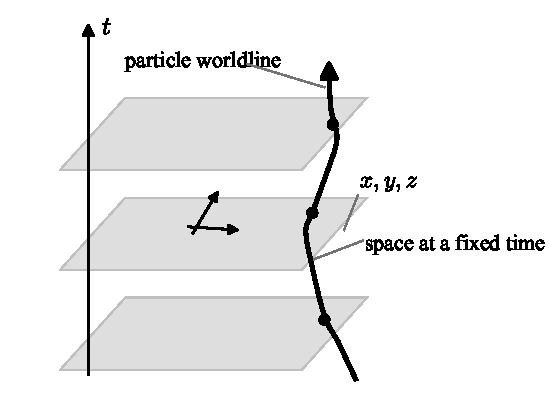
\includegraphics[width=0.72\textwidth]{fig_1.1.pdf}
\caption*{图 1.1\quad 在Newton时空中存在一种绝对的切片，把不同时刻的空间切成各不相同的拷贝。粒子世界线被约束只能随时间向前运动，但能以任意速度穿越空间；对于空间中不同地点的两个事件是否发生在同一时刻这个问题，存在人人一致的答案。}
\end{figure}

\textbf{时空}（spacetime）是一个四维集合，其元素由三个空间维度和一个时间维度来标记。（下一章我们会更严格地处理这些定义。）时空中的单独一个点称为一个\textbf{事件}（event）。粒子的路径是穿过时空的一条曲线，即一个参数化的一维事件集合，称为\textbf{世界线}（worldline）。这样的描述对SR和Newton力学同样适用。无论哪种情形，“时间”所受的对待显然与“空间”有些不同；具体地说，粒子总是沿时间向前行进，而在空间中却可以自由地来回移动。

然而，SR中粒子可以走的路径集合与Newton理论中的相比，有一个重要差别。在Newton力学中，时空有一个基本划分，分成轮廓分明的“固定时刻的全部空间”切片。\emph{同时性}（simultaneity）的观念——两个事件发生在同一时刻——是毫不含糊地定义了的。粒子的轨迹在时间上永远向前，但除此之外不受约束；特别是，两个这类粒子之间的相对速度没有上限。

在SR中，情况发生了戏剧性的改变：特别是，\emph{两个分离的事件“在同时”发生，这一观念没有良定义。}这并不是说时空完全没有什么结构。毋宁说，在每个事件处我们都可以定义一个\textbf{光锥}（light cone），它是穿过时空的那些路径的轨迹，这些路径可能被穿过该事件的光线所取。Newton力学中把时空唯一地切成由时间参数化的空间切片的那种绝对划分，被一条规则取代：物理粒子不能跑得比光快，因而其运动路径始终留在这些光锥之内。

\begin{figure}[H]
\centering
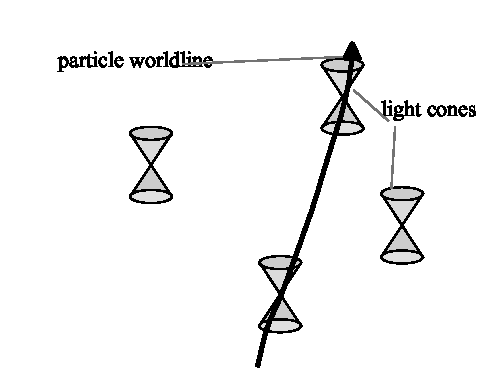
\includegraphics[width=0.72\textwidth]{fig_1.2.pdf}
\caption*{图 1.2\quad 在狭义相对论中，不存在"某一时刻的全部空间"这种绝对观念。取而代之的是一条规则：粒子永远以不大于光速的速率行进。于是我们可以在每个事件处定义光锥，它们局域地刻画了允许轨迹的集合。对于彼此的光锥之外的两个事件，哪个事件在时间上先发生，没有普适的观念。}
\end{figure}

SR中不存在偏好的时间切分，这正是时空观念在此语境中比在Newton力学中更为根本的关键所在。当然，我们可以在时空中选取具体的坐标系，而且一旦选定，在这个特定系统中谈论分离的事件取相同的时间坐标值就是有意义的；但还会存在其他可能的坐标系，它们通过把空间和时间相互“旋转”而与第一组相联系。这一现象是欧几里得几何中旋转的自然推广，我们现在就转向它。

考虑一块最寻常不过的二维平面。给这种平面上的点做标记，通常方便的做法是引入坐标，例如定义正交的$x$轴和$y$轴，按通常方式把每个点投影到这两个轴上。然而，显然关于这个平面的大多数有趣的几何事实都与我们坐标的选取无关；不存在任何偏好的方向。作为一个简单的例子，我们可以考虑两点之间的距离，它由下式给出：

\begin{equation*}
(\Delta s)^2 = (\Delta x)^2 + (\Delta y)^2.
\tag{1.7}
\end{equation*}

在一个不同的笛卡尔坐标系——由相对原来的轴旋转过的$x'$轴和$y'$轴定义——之中，距离的公式丝毫未变：

\begin{equation*}
(\Delta s)^2 = (\Delta x')^2 + (\Delta y')^2.
\tag{1.8}
\end{equation*}

因此我们说，距离在这样的坐标变更下不变。

\begin{figure}[H]
\centering
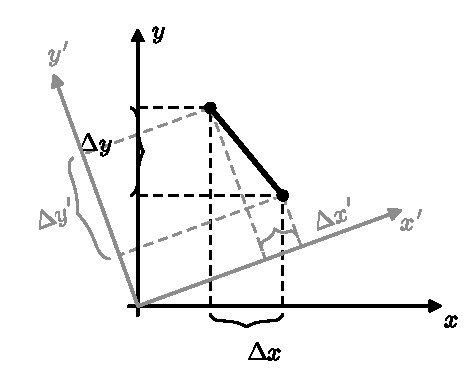
\includegraphics[width=0.72\textwidth]{fig_1.3.pdf}
\caption*{图 1.3\quad 二维欧几里得空间，画有两个不同的坐标系。"两点之间的距离"这类观念与所选的坐标系无关。}
\end{figure}

这就是为什么把平面看作一个内禀的二维空间是有用的，而不是把它看作两个被任意拼到一起的、从根本上不同的一维空间：虽然我们用两个不同的数来标记每个点，这些数并不是几何的本质，因为我们可以在保持距离不变的同时把轴相互旋转。在Newton物理学中，空间和时间却不是这样；把空间和时间相互旋转没有什么有用的含义。相反，“单一时刻的全部空间”这一观念具有独立于坐标的意义。

SR则是另一回事。让我们考虑时空上的坐标$(t,x,y,z)$，按如下方式建立。空间坐标$(x,y,z)$构成一个标准的笛卡尔系，例如可以把相交成直角的刚性杆焊接在一起来构造。这些杆必须自由运动、不受加速。时间坐标由一组时钟定义，这些时钟相对于空间坐标不运动。（既然这是思想实验，我们可以想象这些杆无限长，而且空间中每个点都有一只时钟。）这些时钟按下述意义同步。想象我们从空间中的点1沿直线以恒定速度$c$发送一束光到点2，然后立即回到1（速度为$-c$）。那么，光束到达点2时坐标钟上的时间（记作$t_2$），应当介于光束离开点1时坐标钟上的时间（$t_1$）与它回到同一只钟时的时间（$t_1'$）的正中间：

\begin{equation*}
t_2 = \frac{1}{2}(t_1' + t_1).
\tag{1.9}
\end{equation*}

如此构造出来的坐标系称为一个\textbf{惯性系}（inertial frame），或简称“惯性坐标”。这些坐标是空间中笛卡尔（正交归一）坐标向时空的自然推广。（如此小心翼翼地构造，是为了我们只在\emph{局域}上作比较；例如，绝不在同一时刻去比较两只相距遥远的钟。等到进入广义相对论，这种谨慎将变得更加必要，因为在那里将没有任何办法在整个时空上构造惯性坐标。）

\begin{figure}[H]
\centering
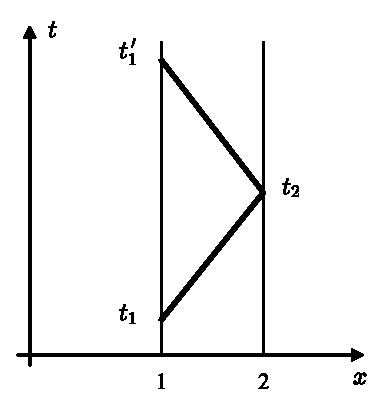
\includegraphics[width=0.72\textwidth]{fig_1.4.pdf}
\caption*{图 1.4\quad 在惯性坐标系中校准时钟。当一束光从点1射向点2再反弹回来时，如果时间$t_2$恰好位于$t_1$与$t_1'$的正中间，这些钟就是同步的。}
\end{figure}

我们可以用这套流程构造任意多个惯性系，它们与第一个的差别在于初始位置和时间的偏移、角度以及（恒定的）速度。在Newton式的世界里，新坐标$(t',x',y',z')$会有这样的特点：$t'=t+\text{常数}$，与空间坐标无关。也就是说，“两个事件同时发生，即在同一时刻发生”有一个绝对的含义。但在SR中这并不成立；一般而言，由$t=\text{常数}$定义的三维“空间”将不同于由$t'=\text{常数}$定义的那些。

不过，我们并没有完全坠入混乱。暂且不加任何动机，考虑一下我们将称之为两个事件之间的\textbf{时空间隔}（spacetime interval）的东西：

\begin{equation*}
\boxed{(\Delta s)^2 = -(c\Delta t)^2 + (\Delta x)^2 + (\Delta y)^2 + (\Delta z)^2.}
\tag{1.10}
\end{equation*}

（注意，即使对两个不重合的点，它也可以为正、为负或为零。）这里的$c$是空间与时间之间某个固定的换算因子，也就是说，一个固定的速度。作为经验事实，电磁波恰以这个速度$c$在真空中传播，因此我们把它称作“光速”。然而，重要的并不是光子碰巧以这个速率行进，而是存在这样一个$c$，使得\emph{时空间隔在惯性坐标的变更下不变}。换句话说，如果我们建立一个新的惯性系$(t',x',y',z')$，间隔将具有同样的形式：

\begin{equation*}
(\Delta s)^2 = -(c\Delta t')^2 + (\Delta x')^2 + (\Delta y')^2 + (\Delta z')^2.
\tag{1.11}
\end{equation*}

这正是为什么把SR看作四维时空的理论是有意义的，这个四维时空称为\textbf{Minkowski 空间}（Minkowski space）。（它是四维流形的一个特殊情形，流形我们稍后会详细处理。）我们将会看到，我们已经隐式定义的那些坐标变换，确实在某种意义上把空间和时间相互旋转。不存在“同时事件”的绝对观念；两件事是否发生在同一时刻，取决于所用的坐标。因此，把 Minkowski 空间分割成空间和时间，是我们为自己的目的而做的选择，并不是情形本身固有的东西。

与SR相联系的“佯谬”几乎全部源于对Newton观念的顽固固守：坚持存在唯一的时间坐标，坚持存在“单一时刻的全部空间”。改用时空来思考，而不是把空间与时间合在一起思考，这些佯谬往往就会消失。

让我们引入一些方便的记号。时空上的坐标将用带希腊字母上标指标的字母来表示，指标从0取到3，其中0一般表示时间坐标。于是，

\begin{equation*}
x^{\mu}:\quad
\begin{aligned}
x^0 &= ct \\
x^1 &= x \\
x^2 &= y \\
x^3 &= z.
\end{aligned}
\tag{1.12}
\end{equation*}

（不要开始把这些上标当成幂指数。）此外，为简单起见，我们将选取使下式成立的单位制：

\begin{equation*}
c = 1;
\tag{1.13}
\end{equation*}

因此在后面所有的公式里，我们都将省去因子$c$。经验告诉我们，$c$为$3\times10^8$米每秒；于是，我们是在1秒等于$3\times10^8$米的单位制下工作。有时分别指称$x^\mu$的空间分量和时间分量会很有用，所以我们将用拉丁字母上标单独表示空间分量：

\begin{equation*}
x^{i}:\quad
\begin{aligned}
x^1 &= x \\
x^2 &= y \\
x^3 &= z.
\end{aligned}
\tag{1.14}
\end{equation*}

把时空间隔写成更紧凑的形式也很方便。为此我们引入一个$4\times4$矩阵，即\textbf{度规}（metric），用两个下标书写：

\begin{equation*}
\eta_{\mu\nu} =
\begin{pmatrix}
-1 & 0 & 0 & 0 \\
0 & 1 & 0 & 0 \\
0 & 0 & 1 & 0 \\
0 & 0 & 0 & 1
\end{pmatrix}.
\tag{1.15}
\end{equation*}

（一些文献——尤其是场论教材——用相反的符号定义度规，所以要当心。）于是我们有漂亮的公式

\begin{equation*}
(\Delta s)^2 = \eta_{\mu\nu}\Delta x^\mu \Delta x^\nu.
\tag{1.16}
\end{equation*}

\begin{figure}[H]
\centering
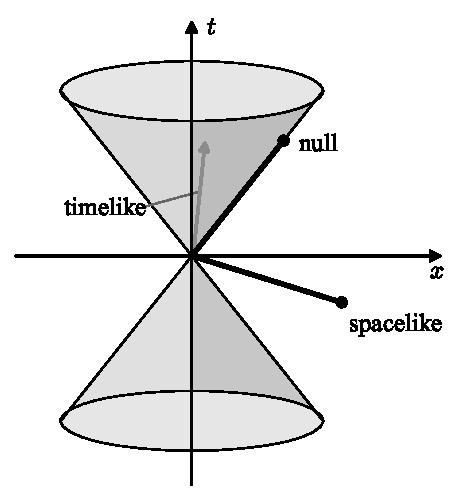
\includegraphics[width=0.72\textwidth]{fig_1.5.pdf}
\caption*{图 1.5\quad 画在时空图上的一个光锥。图中标出了与原点类空分离、类光分离和类时分离的点。}
\end{figure}

这个公式引入了\textbf{求和约定}（summation convention）：既作为上标又作为下标出现的指标要对之求和。我们把这样的指标称为\textbf{哑指标}（dummy indices）；必须记住，它们对所有可能的值求和，而不取任何特定的值。（情形将永远如此：哑指标严格成对出现，一个“在上”，一个“在下”。这一点以后再谈。）因此，式 (1.16) 的内容与式 (1.10) 完全相同。

\textbf{时空图}（spacetime diagram）是一种极其有用的工具，那就让我们从这个观点来考察 Minkowski 空间。我们可以先把起初的$t$轴与$x$轴画成直角，并隐去$y$轴和$z$轴。（时空图上画出的“直角”并不必然意味着“在时空中正交”，尽管在这个例子里，$t$轴与$x$轴恰好确实正交。）考察以速率$c=1$行进的路径颇有启发，这些路径由$x=\pm t$给出。由以光速行进的直线与单个事件相连的全部点的集合，就是\textbf{光锥}；因为如果想象再纳入一个空间维度，那两条对角线就会补全成一个锥面。光锥天然分为未来光锥与过去光锥；一点$p$的未来与过去光锥内部所有点的集合，称为与$p$\textbf{类时分离}（timelike separated）；光锥之外的点与$p$\textbf{类空分离}（spacelike separated）；而恰好位于锥面上的点，则与$p$\textbf{类光分离}（lightlike or null separated）。回到式 (1.10)，我们看到类时分离的点之间的间隔为负，类空分离的点之间的间隔为正，类光分离的点之间的间隔为零。（间隔定义为$(\Delta s)^2$本身，而不是这个量的平方根。）

间隔对类时曲线（比光慢的粒子实际上将沿之运动）为负，这件事有些恼人，所以我们定义\textbf{固有时}（proper time）$\tau$满足

\begin{equation*}
(\Delta\tau)^2 = -(\Delta s)^2 = -\eta_{\mu\nu}\Delta x^\mu \Delta x^\nu.
\tag{1.17}
\end{equation*}

时空间隔的一个关键性质是：\emph{两个事件之间的固有时，量度的是沿连接这两事件的直线路径运动的观者所经历的时间。}这在非常特殊的情形下最容易看清：两个事件具有相同的空间坐标，只在时间上分离；这对应于在两事件之间旅行的观者相对所用坐标系静止。于是$(\Delta\tau)^2=-\eta_{\mu\nu}\Delta x^\mu\Delta x^\nu=(\Delta t)^2$，故$\Delta\tau=\Delta t$；当然，我们本来就把$t$定义为位于固定空间位置上的钟所量度的时间。但时空间隔在惯性系的变更下不变；因此，两个固定事件之间的固有时 (1.17) 在观者运动着的惯性系中求出的值，与在观者静止的惯性系中求出的值相同。

一个关键的事实是：对更一般的轨迹，固有时与坐标时并不相同（尽管固有时总是沿轨迹运动的观者所携带的钟量度的时间）。考虑连接事件$A$和$C$的两条轨迹：一条是直线，经过标记为$B$的中点；另一条由一位观者走完，他以恒定速度$v=dx/dt$从$A$离开行进到一点$B'$，再以恒定速度$-v$返回，与前者相交于事件$C$。

\begin{figure}[H]
\centering
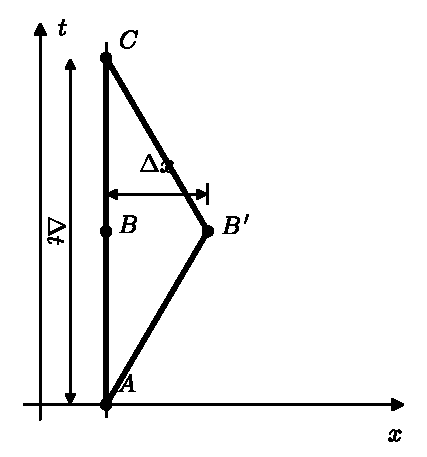
\includegraphics[width=0.72\textwidth]{fig_1.6.pdf}
\caption*{图 1.6\quad 双生子佯谬。沿穿过时空的直线路径$ABC$旅行的行者，将比沿非直线路径$AB'C$旅行的人衰老得更多。既然固有时是穿过时空走过的距离的量度，这应当不足为怪。（唯一可能令人惊讶的是，直线路径竟然是固有时\emph{最长}的那一条；这可以追溯到度规类时分量的负号。）}
\end{figure}

选取惯性坐标，使直的轨迹描述一个静止不动的粒子，事件$A$位于坐标$(t,x)=(0,0)$，$C$位于$(\Delta t,0)$。两条路径于是在时空中构成一个等腰三角形；$B$的坐标为$(\frac{1}{2}\Delta t,0)$，$B'$的坐标为$(\frac{1}{2}\Delta t,\Delta x)$，其中$\Delta x=\frac{1}{2}v\Delta t$。显然有$\Delta\tau_{AB}=\frac{1}{2}\Delta t$，但是

\begin{equation*}
\begin{aligned}
\Delta\tau_{AB'} &= \sqrt{\left(\tfrac{1}{2}\Delta t\right)^2 - (\Delta x)^2} \\
&= \tfrac{1}{2}\sqrt{1-v^2}\,\Delta t.
\end{aligned}
\tag{1.18}
\end{equation*}

应当显然有$\Delta\tau_{BC}=\Delta\tau_{AB}$和$\Delta\tau_{B'C}=\Delta\tau_{AB'}$。于是，沿直线从事件$A$旅行到$C$的观者经历的时间流逝为$\Delta\tau_{ABC}=\Delta t$，而走出去又返回的那位经历的却是

\begin{equation*}
\Delta\tau_{AB'C} = \sqrt{1-v^2}\,\Delta t < \Delta t.
\tag{1.19}
\end{equation*}

尽管两位观者在时空中的同一点出发、又在同一点结束，他们衰老的程度却不一样。这就是著名的“双生子佯谬”（twin paradox）——形形色色的误解和蹩脚解释的不幸上演之处。真相很直接：时空中的非直线路径与直线路径有不同的间隔，正如空间中的非直线路径与直线路径有不同的长度。当然，这件事并不像听起来那么平凡；深刻的洞见在于“沿世界线流逝的时间”以何种方式与穿过时空历经的间隔相联系。在Newton式的世界里，坐标$t$代表贯穿全部时空的普适的时间之流；在相对论中，$t$只是一个方便的坐标，时间的流逝取决于你沿哪条路径旅行。一个重要的区别是：非直线路径的固有时\emph{更短}。在空间中，两点之间最短的距离是直线；在时空中，两事件之间最长的固有时属于直的轨迹。

并非所有轨迹都齐整到可以由直线段拼成。在更一般的情形下，引入无穷小间隔，即\textbf{线元}（line element），会很有用：

\begin{equation*}
\boxed{ds^2 = \eta_{\mu\nu}dx^\mu dx^\nu,}
\tag{1.20}
\end{equation*}

其中$dx^\mu$是无穷小的坐标位移。（我们这里的处理相当不正式，不过以后会补正。）从这个定义出发，人们很想取平方根并沿一条路径积分，以得到有限的间隔，但$\int\sqrt{\eta_{\mu\nu}dx^\mu dx^\nu}$究竟应当是什么意思，多少有些不清楚。换一种做法，我们把穿过时空的一条路径看作参数化曲线$x^\mu(\lambda)$。注意，与Newton力学的传统做法不同，参量$\lambda$不一定等同于时间坐标。于是我们可以计算导数$dx^\mu/d\lambda$，并把沿类空曲线（无穷小间隔为类空的曲线）的路径长度写作

\begin{equation*}
\Delta s = \int \sqrt{\eta_{\mu\nu}\frac{dx^\mu}{d\lambda}\frac{dx^\nu}{d\lambda}}\,d\lambda,
\tag{1.21}
\end{equation*}

其中积分沿整条路径进行。对类时路径我们用固有时

\begin{equation*}
\Delta\tau = \int \sqrt{-\eta_{\mu\nu}\frac{dx^\mu}{d\lambda}\frac{dx^\nu}{d\lambda}}\,d\lambda,
\tag{1.22}
\end{equation*}

它将为正。（对类光路径，间隔干脆就是零。）当然，我们可以考虑在一些地方类时、在另一些地方类空的路径，但幸运的是很少有必要，因为物理粒子的路径从不改变其特征（有质量粒子沿类时路径运动，无质量粒子沿类光路径运动）。再说一遍，$\Delta\tau$确实就是沿轨迹运动的观者所量度的时间。

狭义相对论中的\emph{加速度}（acceleration）这一概念名声不佳，但毫无道理。在建立惯性坐标时，我们\emph{当然}小心翼翼地确保了在此类坐标中静止的粒子不受加速。然而，一旦建立了这样的坐标，我们就可以随意考虑物理粒子的任何轨迹，无论加速与否。特别是，“SR处理不了加速轨迹、必须请出广义相对论”的传言毫无事实依据。广义相对论是在有引力之时、当时空变得弯曲之际才变得相关。平直时空中的任何过程都在狭义相对论的框架内得到描述；特别地，像式 (1.22) 这样的表达式是完全普遍的。

% 1.3 Lorentz Transformations
\section{洛伦兹变换}

现在，我们可以在比之前稍抽象一点的层次上考虑时空中的坐标变换。我们感兴趣的是如何把经由上述流程构造的各种惯性系联系起来，并对此给出一个形式化的描述；也就是说，（考虑那些）使间隔 (1.16) 保持不变的坐标系。其中简单的一类是\textbf{平移}（translations），它们只是让坐标平移（在空间或时间上）：

\begin{equation*}
x^\mu \rightarrow x^{\mu'} = \delta^{\mu'}_{\mu}\,(x^\mu + a^\mu),
\tag{1.23}
\end{equation*}

其中$a^\mu$是由四个固定数构成的一组数，而$\delta^{\mu'}_{\mu}$是传统Kronecker delta符号的四维版本：

\begin{equation*}
\delta^{\mu'}_{\mu} =
\begin{cases}
1 & \text{当 } \mu' = \mu, \\
0 & \text{当 } \mu' \neq \mu.
\end{cases}
\tag{1.24}
\end{equation*}

注意，我们把撇号加在指标上，而不是加在$x$上。这样做的理由，等我们开始同矢量和张量打交道之后会变得更加清楚；这种记号提醒我们：几何对象是同一个，只是它的分量是相对于另一个坐标系分解的。平移保持差值$\Delta x^\mu$不变，所以间隔不变并不令人惊讶。其他相关的变换还包括空间的\textbf{旋转}（rotations），以及以一个恒定速度矢量做的偏移，即\textbf{推动}（boosts）；这些都是线性变换，可以用一个（不依赖时空的）矩阵去乘$x^\mu$来描述：

\begin{equation*}
x^{\mu'} = \Lambda^{\mu'}{}_{\nu}x^\nu,
\tag{1.25}
\end{equation*}

或者，用更传统的矩阵记号，

\begin{equation*}
x' = \Lambda x.
\tag{1.26}
\end{equation*}

（我们一般会使用指标，而不是矩阵记号，但此刻我们有意把这里的讨论与通常用矩阵描述的某些其他熟悉概念联系起来。）这些变换并不使差值$\Delta x^\mu$保持不变，而是把它们再乘上矩阵$\Lambda$。什么样的矩阵能使间隔不变？坚持用矩阵记号的话，我们想要的是

\begin{equation*}
\begin{aligned}
(\Delta s)^2 &= (\Delta x)^{\mathrm{T}}\eta(\Delta x) = (\Delta x')^{\mathrm{T}}\eta(\Delta x') \\
&= (\Delta x)^{\mathrm{T}}\Lambda^{\mathrm{T}}\eta\Lambda(\Delta x),
\end{aligned}
\tag{1.27}
\end{equation*}

因此

\begin{equation*}
\eta = \Lambda^{\mathrm{T}}\eta\Lambda,
\tag{1.28}
\end{equation*}

% 本文件至此为止：书页12末句止于式 (1.28) 后的逗号，正文延续到书页13，由下一块（ch1_b）接续。
或
\begin{equation*}
\eta_{\rho\sigma}=\Lambda^{\mu'}{}_{\rho}\,\eta_{\mu'\nu'}\,\Lambda^{\nu'}{}_{\sigma}
=\Lambda^{\mu'}{}_{\rho}\Lambda^{\nu'}{}_{\sigma}\eta_{\mu'\nu'}\,.
\tag{1.29}
\end{equation*}

（在矩阵记号中次序是重要的，而在指标记号中则无关紧要。）我们想要找出矩阵$\Lambda^{\mu'}{}_{\nu}$，使得矩阵$\eta_{\mu'\nu'}$的分量与$\eta_{\rho\sigma}$的分量相同；这就是间隔在这些变换下不变的含义。

满足式(1.28)的那些矩阵称为\textbf{洛伦兹变换}（Lorentz transformations）；它们的全体在矩阵乘法下构成一个群，称为\textbf{洛伦兹群}（Lorentz group）。这个群与SO(3)——三维空间中的转动群——之间有着密切的类比。转动群可以看成由满足$R^{\mathrm{T}}\mathbf{1}R=\mathbf{1}$的$3\times3$矩阵$R$组成，其中$\mathbf{1}$是$3\times3$单位矩阵。这样的矩阵称为\emph{正交}（orthogonal）矩阵，$3\times3$的这种矩阵构成群O(3)。其中不仅有转动，还包括空间坐标轴取向的反转（\textbf{宇称变换}（parity transformations））。有时我们还想排除宇称变换，于是进一步要求矩阵的行列式为1（$|R|=1$）；这样的矩阵称为\emph{特殊}（special）矩阵，所得的群就是SO(3)。如果把它写成

\begin{equation*}
\mathbf{1}=R^{\mathrm{T}}\mathbf{1}R\,,
\tag{1.30}
\end{equation*}

正交条件看上去就更像式(1.28)了。

于是，转动群O(3)与洛伦兹群的差别就在于：把$\mathbf{1}$——所有元素都等于$+1$的$3\times3$对角矩阵——换成$\eta$，一个对角元一个为$-1$、其余为$+1$的$4\times4$对角矩阵。因此洛伦兹群常被称作O(3,1)。它不仅包含推动和转动，还包含时间方向的分立反转以及宇称变换。和前面一样，我们可以要求$|\Lambda|=1$，得到“固有洛伦兹群”（proper Lorentz group）SO(3,1)。然而这并没有给我们真正想要的东西，即连续洛伦兹变换的集合（那些与恒等变换光滑连通的变换），因为时间反转与宇称反转的组合会具有单位行列式。从式(1.29)的$(\rho,\sigma)=(0,0)$分量出发，我们容易证明$|\Lambda^{0'}{}_{0}|\geq1$，其中负值对应时间反转。因此我们最终可以再要求$\Lambda^{0'}{}_{0}\geq1$（加上$|\Lambda|=1$），得到“固有正向”（proper orthochronous）或“受限”（restricted）洛伦兹群。有时它被记作类似$SO(3,1)\uparrow$的符号，但通常我们不会费心去明确作出这种区分。注意，$3\times3$单位矩阵其实就是普通平直空间的度规。所有本征值都为正的这种度规称为\textbf{欧几里得型}（Euclidean）度规，而像式(1.15)那样只带一个负号的度规则称为\textbf{洛伦兹型}（Lorentzian）度规。

写下简单洛伦兹变换的显式表达式是直截了当的。$x$-$y$平面中一个我们熟悉的转动是

\begin{equation*}
\Lambda^{\mu'}{}_{\nu}=
\begin{pmatrix}
1 & 0 & 0 & 0\\
0 & \cos\theta & \sin\theta & 0\\
0 & -\sin\theta & \cos\theta & 0\\
0 & 0 & 0 & 1
\end{pmatrix}.
\tag{1.31}
\end{equation*}

转动角$\theta$是周期为$2\pi$的周期变量。推动则可以想成“空间方向与时间方向之间的转动”。沿$x$方向的推动就是一个例子：

\begin{equation*}
\Lambda^{\mu'}{}_{\nu}=
\begin{pmatrix}
\cosh\phi & -\sinh\phi & 0 & 0\\
-\sinh\phi & \cosh\phi & 0 & 0\\
0 & 0 & 1 & 0\\
0 & 0 & 0 & 1
\end{pmatrix}.
\tag{1.32}
\end{equation*}

推动参量$\phi$与转动角不同，其定义范围是从$-\infty$到$\infty$。把各个变换相乘就可以得到一般的变换；这个六参数矩阵（三个推动、三个转动）的显式表达式并不好看，也不值得费神写下来。一般说来洛伦兹变换不可对易，所以洛伦兹群是非阿贝尔群（nonabelian）。平移与洛伦兹变换合在一起构成一个十参数非阿贝尔群，即\textbf{庞加莱群}（Poincaré group）。

大家得知推动对应于通过换到一个以恒定速度运动的参考系来改变坐标时，不应感到惊讶，但我们不妨更明白地看一下。（不要把“推动”（boosting）与“加速”（accelerating）混淆。变到一个不同参考系的推动与加速一个物体这两者之间的差别，就如同转到不同坐标系与让物体自旋这两者之间的差别。）对于由式(1.32)给出的变换，变换后的坐标$t'$和$x'$将为

\begin{align*}
t'&=t\cosh\phi-x\sinh\phi\\
x'&=-t\sinh\phi+x\cosh\phi\,.
\tag{1.33}
\end{align*}

由此我们看到，由$x'=0$定义的那个点在运动；它具有速度

\begin{equation*}
v=\frac{x}{t}=\frac{\sinh\phi}{\cosh\phi}=\tanh\phi\,.
\tag{1.34}
\end{equation*}

为了换成更平实的记号，我们可以代入$\phi=\tanh^{-1}v$，得到

\begin{align*}
t'&=\gamma(t-vx)\\
x'&=\gamma(x-vt)\,,
\tag{1.35}
\end{align*}

其中$\gamma=1/\sqrt{1-v^{2}}$。的确如此，我们这条抽象路线重新得到了洛伦兹变换的惯用表达式。应用这些公式就得到时间膨胀（time dilation）、长度收缩（length contraction）等等。

在时空图（spacetime diagram）的语境中考察洛伦兹变换是很有启发性的。根据式(1.33)，在$x$-$t$平面内的推动下，$x'$轴（$t'=0$）由$t=x\tanh\phi$给出，而$t'$轴（$x'=0$）则由$t=x/\tanh\phi$给出。于是我们看到，空间轴和时间轴彼此向对方转过去，只不过它们像剪刀一样斜着合拢，而不再保持传统欧几里得意义下的正交。（我们将会看到，这些轴事实上在洛伦兹意义下确实仍保持正交；这正是度规在推动下保持不变的含义。）

\begin{figure}[H]
\centering
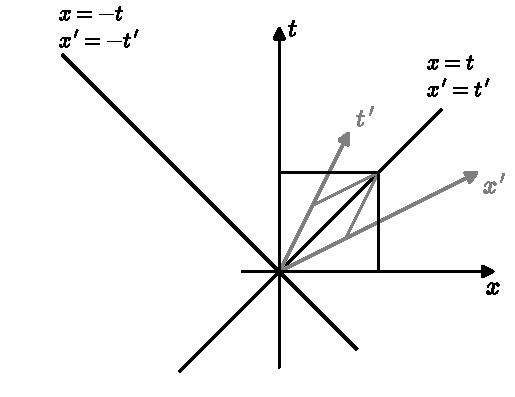
\includegraphics[width=0.72\textwidth]{fig_1.7.pdf}
\caption*{图 1.7\quad 洛伦兹变换把$\{t',x'\}$坐标与$\{t,x\}$坐标联系起来。注意光锥不变。}
\end{figure}

这应该毫不奇怪，因为假如时空的行为就像四维版本的空间，那世界将会是一个非常不同的地方。我们相当鲜明地看到了这种情形与Newton世界之间的区别；在狭义相对论中，我们不可能（以不依赖于坐标的方式）说出一个与点$p$类空间隔的点究竟是在$p$的未来、$p$的过去，还是“与$p$同时”。

还要注意，由$x'=\pm t'$定义的路径与由$x=\pm t$定义的路径完全相同；这些轨迹在沿$x$轴的推动下保持不变。当然，我们知道光正是以这个速度传播的；于是我们便发现，光速在任何惯性系中都是相同的。

\section{矢量}

要更细致地探究 Minkowski 空间的结构，就需要引入矢量与张量的概念。我们先从矢量讲起，大家应该对它已经熟悉。当然，时空中的矢量是四维的，常被称为\textbf{四维矢量}（four-vectors）。这会带来相当可观的差别——例如，两个四维矢量之间根本不存在叉积这种东西。

除了维数这个简单事实之外，最需要强调的一点是：每个矢量都定域在时空中的一个给定点上。你可能习惯于把矢量看成从空间中一点拉伸到另一点的东西，甚至看成可以随意从一个点滑动到另一个点的“自由”矢量。在平直空间的语境之外，这些都不是有用的概念；一旦引入曲率，我们就失去了从一个点向另一个点画出特殊曲线的能力，也失去了把矢量唯一地搬动绕行流形的能力。毋宁说，对时空中的每个点$p$，我们都把定域于该点的所有可能矢量的集合与它联系起来；这个集合称为$p$处的\textbf{切空间}（tangent space），记作$T_p$。这个名称的灵感来自这样的图像：在一个简单的弯曲二维空间中，附着于某点的那些矢量全体构成一个在该点与此空间相切的平面。（这幅图像依赖于把流形和切空间嵌入一个更高维的外部空间，而一般来说我们既没有也不需要这种嵌入。）抛开这个灵感不谈，重要的是把这些矢量看成定域于单独一点，而不是从一点拉伸到另一点（尽管这不会妨碍我们在时空图上把它们画成箭头）。

在第2章中，我们将把每个点处的切空间与我们可以从时空本身构造出来的东西联系起来。眼下，只需把$T_p$想成时空每一点上的一个抽象矢量空间。所谓\textbf{（实）矢量空间}（real vector space），是指由一些对象（矢量）组成的集合，它们可以线性地彼此相加并乘以实数。于是，对任意两个矢量$V$、$W$和实数$a$、$b$，我们有

\begin{equation*}
(a+b)(V+W)=aV+bV+aW+bW\,.
\tag{1.36}
\end{equation*}

每个矢量空间都有一个原点，即在矢量加法下充当恒等元的零矢量。在许多矢量空间中还有别的运算，比如取内积（点积），但这是矢量空间这一初等概念之外的额外结构。

矢量是一个定义得非常明确的几何对象，\textbf{矢量场}（vector field）也一样，它定义为在时空每一点上恰好有一个矢量的矢量的集合。[把一个$n$维流形$M$的所有切空间汇集起来，可以组装成一个$2n$维流形，称为\textbf{切丛}（tangent bundle），$T(M)$。它是“纤维丛”（fiber bundle）的一个具体例子，纤维丛还带有某种额外的数学结构；就目前的目的我们不需要那些细节。]尽管如此，把矢量相对于某组基矢分解成分量往往是有用的。\textbf{基}（basis）是任何一组既张满矢量空间（任何矢量都是基矢的线性组合）又线性无关（基中没有任何一个矢量是其余基矢的线性组合）的矢量。对任何给定的矢量空间，可供选择的基有无穷多种，但每个基都由相同数目的矢量组成，这个数目称为该空间的\textbf{维数}（dimension）。（对于 Minkowski 空间中一点相应的切空间，维数当然是四。）

\begin{figure}[H]
\centering
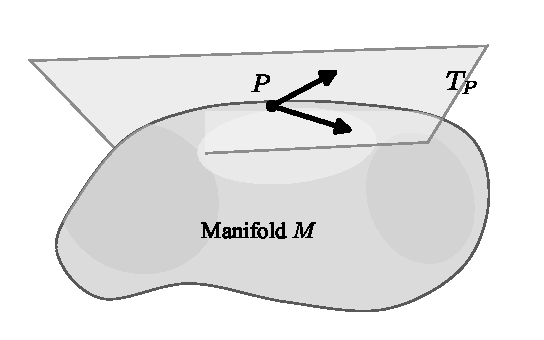
\includegraphics[width=0.72\textwidth]{fig_1.8.pdf}
\caption*{图 1.8\quad 切空间$T_p$的示意性图示——点$p$处所有矢量构成的空间。}
\end{figure}

设想在每个切空间中都立起一组四个矢量$\hat{e}_{(\mu)}$作为基，$\mu$和通常一样取遍$\{0,1,2,3\}$。实际上，不妨说每个基都是“适配于坐标$x^\mu$”的——也就是说，基矢$\hat{e}_{(1)}$就是我们通常认为指向$x$轴方向的那个矢量。我们完全没有必要选择适配于任何坐标系的基，尽管这样做往往很方便。（和前面一样，我们在这里本可以更精确一些，但后面我们会以令人难以忍受的精确程度重新讨论这个问题，所以现在稍微马虎一点是可以原谅的。）于是，任何抽象矢量$A$都可以写成基矢的线性组合：

\begin{equation*}
A=A^{\mu}\hat{e}_{(\mu)}\,.
\tag{1.37}
\end{equation*}

系数$A^{\mu}$就是矢量$A$的\textbf{分量}（components）。我们多半会把基完全忘掉，而有点随意地把“矢量$A^{\mu}$”挂在嘴边，但要记住这只是一种简写。真正的矢量是抽象的几何实体，而分量只是矢量在某个方便的基下基矢的系数。（由于我们通常会不写出显式基矢，指标一般就用来标记矢量和张量的分量。这就是基矢的指标要加括号的原因——提醒我们这是矢量的集合，而不是单个矢量的分量。）

时空中的一个矢量的标准例子是曲线的切矢量。穿过时空的一条参数化曲线或路径由坐标作为参量的函数给出，例如$x^{\mu}(\lambda)$。切矢量$V(\lambda)$的分量为

\begin{equation*}
V^{\mu}=\frac{\mathrm{d}x^{\mu}}{\mathrm{d}\lambda}\,.
\tag{1.38}
\end{equation*}

完整的矢量是$V=V^{\mu}\hat{e}_{(\mu)}$。在洛伦兹变换下，坐标$x^{\mu}$按照式(1.25)变换，而参量化$\lambda$不变；因此我们可以推出，切矢量的分量必须按如下方式变化

\begin{equation*}
\boxed{\,V^{\mu}\rightarrow V^{\mu'}=\Lambda^{\mu'}{}_{\nu}V^{\nu}\,.}
\tag{1.39}
\end{equation*}

然而，矢量$V$本身（与其在某个坐标系中的分量相对而言）在洛伦兹变换下是不变的。我们可以利用这个事实来导出基矢的变换性质。把变换后坐标系中的那组基矢记为$\hat{e}_{(\nu')}$。由于矢量不变，我们有

\begin{equation*}
V=V^{\mu}\hat{e}_{(\mu)}=V^{\nu'}\hat{e}_{(\nu')}
=\Lambda^{\nu'}{}_{\mu}V^{\mu}\hat{e}_{(\nu')}\,.
\tag{1.40}
\end{equation*}

但无论分量$V^{\mu}$的数值是什么，这个关系都必须成立。因此我们可以说

\begin{equation*}
\hat{e}_{(\mu)}=\Lambda^{\nu'}{}_{\mu}\hat{e}_{(\nu')}\,.
\tag{1.41}
\end{equation*}

要把新基$\hat{e}_{(\nu')}$用旧基$\hat{e}_{(\mu)}$表示出来，我们应该乘以洛伦兹变换$\Lambda^{\nu'}{}_{\mu}$的逆。但是，从无撇坐标变到带撇坐标的洛伦兹变换的逆也是一个洛伦兹变换，只不过这次是从带撇系变到无撇系。因此我们将引入一种略显精妙的记号：对这两个矩阵用同一个符号，只是把带撇指标与无撇指标互换。也就是说，由$\Lambda^{\mu'}{}_{\nu}$规定的洛伦兹变换，其逆变换写作$\Lambda^{\rho}{}_{\sigma'}$。从运算上讲，这意味着

\begin{equation*}
\Lambda^{\mu}{}_{\nu'}\Lambda^{\nu'}{}_{\rho}=\delta^{\mu}{}_{\rho}\,,\qquad
\Lambda^{\sigma'}{}_{\lambda}\Lambda^{\lambda}{}_{\tau'}=\delta^{\sigma'}{}_{\tau'}\,.
\tag{1.42}
\end{equation*}

于是由式(1.41)我们得到基矢的变换规则：

\begin{equation*}
\hat{e}_{(\nu')}=\Lambda^{\mu}{}_{\nu'}\hat{e}_{(\mu)}\,.
\tag{1.43}
\end{equation*}

因此，基矢的集合按坐标或矢量分量的洛伦兹变换之逆来变换。

让我们稍停片刻，把这一切消化一下。我们引入了用上指标标记的坐标，它们在洛伦兹变换下按某种方式变换。接着我们考虑了也用上指标写出的矢量分量，这是有意义的，因为它们以与坐标函数相同的方式变换。（在固定的坐标系中，四个坐标$x^{\mu}$中的每一个都可以看成时空上的函数，矢量场的四个分量中的每一个也是如此。）与坐标系相联系的基矢则通过逆矩阵变换，并用下指标标记。这种记号保证了由分量与基矢求和构造出来的不变对象在变换下保持不变，正如我们所愿。如果我说，对于可能有多个指标的张量，情形也将继续如此，大概不算把后面的内容剧透太多。

\section{对偶矢量（1-形式）}

一旦建立了一个矢量空间，我们就可以定义另一个与之相联系的矢量空间（维数相同），称为\textbf{对偶矢量空间}（dual vector space）。对偶空间通常用星号标记，于是切空间$T_p$的对偶空间称为\textbf{余切空间}（cotangent space），记作$T_p^{*}$。对偶空间是从原来的矢量空间到实数的所有线性映射构成的空间；用数学行话说，若$\omega\in T_p^{*}$是一个对偶矢量（dual vector），则它作为一个映射来作用，满足

\begin{equation*}
\omega(aV+bW)=a\omega(V)+b\omega(W)\in\mathbf{R}\,,
\tag{1.44}
\end{equation*}

其中$V$、$W$是矢量，$a$、$b$是实数。这些映射的妙处在于它们本身也构成一个矢量空间；于是，若$\omega$和$\eta$是对偶矢量，我们有

\begin{equation*}
(a\omega+b\eta)(V)=a\omega(V)+b\eta(V)\,.
\tag{1.45}
\end{equation*}

为了让这个构造更具体一点，我们可以引入一组基对偶矢量$\hat{\theta}^{(\nu)}$，办法是要求

\begin{equation*}
\hat{\theta}^{(\nu)}(\hat{e}_{(\mu)})=\delta^{\nu}{}_{\mu}\,.
\tag{1.46}
\end{equation*}

于是每个对偶矢量都可以用它的分量写出，我们用下指标来标记分量：

\begin{equation*}
\omega=\omega_{\mu}\hat{\theta}^{(\mu)}\,.
\tag{1.47}
\end{equation*}

通常，与矢量的情形完全类似，我们会径直写$\omega_{\mu}$，用它代表整个对偶矢量。实际上，你有时会看到$T_p$的元素（就是我们所说的矢量）被称为\textbf{逆变矢量}（contravariant vectors），而$T_p^{*}$的元素（就是我们所说的对偶矢量）被称为\textbf{协变矢量}（covariant vectors），不过在如今这个时代，这些术语听起来有点过时了。只要你把普通矢量称作带上指标的矢量、把对偶矢量称作带下指标的矢量，应该没有人会不高兴。对偶矢量的另一个名字是\textbf{1-形式}（one-forms），这个多少有些神秘的称呼在第2章中会变得更清楚。

分量记号给出了一种书写对偶矢量作用于矢量的简单方式：

\begin{align*}
\omega(V)&=\omega_{\mu}\hat{\theta}^{(\mu)}(V^{\nu}\hat{e}_{(\nu)})\\
&=\omega_{\mu}V^{\nu}\hat{\theta}^{(\mu)}(\hat{e}_{(\nu)})\\
&=\omega_{\mu}V^{\nu}\delta^{\mu}{}_{\nu}\\
&=\omega_{\mu}V^{\mu}\in\mathbf{R}\,.
\tag{1.48}
\end{align*}

这正是我们很少需要把基矢和对偶矢量显式写出来的原因；分量包办了一切工作。式(1.48)的形式还暗示，通过定义

\begin{equation*}
V(\omega)\equiv\omega(V)=\omega_{\mu}V^{\mu}\,.
\tag{1.49}
\end{equation*}

我们可以把矢量看成对偶矢量上的线性映射。因此，对偶矢量空间的对偶空间就是原来的矢量空间本身。

当然，在时空中我们感兴趣的不是一个单独的矢量空间，而是矢量场和对偶矢量场。[把$M$上所有余切空间汇合起来，就得到\textbf{余切丛}（cotangent bundle），$T^{*}(M)$。]在那种情形下，对偶矢量场作用在矢量场上得到的不是一个单独的数，而是时空上的一个\textbf{标量}（scalar）（函数）。标量是不带指标的量，它在洛伦兹变换下不变；它是从时空到实数的、不依赖于坐标的映射。

我们可以用前面处理矢量时用过的同样论证（几何对象独立于坐标，即使它们的分量并非如此）来导出对偶矢量的变换性质。答案是：对于分量，

\begin{equation*}
\boxed{\,\omega_{\mu'}=\Lambda^{\nu}{}_{\mu'}\omega_{\nu}\,,}
\tag{1.50}
\end{equation*}

而对于基对偶矢量，

\begin{equation*}
\hat{\theta}^{(\rho')}=\Lambda^{\rho'}{}_{\sigma}\hat{\theta}^{(\sigma)}\,.
\tag{1.51}
\end{equation*}

这正是从指标位置所能预期的；对偶矢量的分量按矢量分量的逆变换来变换。注意这就保证了标量(1.48)在洛伦兹变换下不变，正如它本应如此。

在时空中，对偶矢量最简单的例子是标量函数的\textbf{梯度}（gradient），即对时空坐标的偏导数的集合，我们用小写的d来记它：

\begin{equation*}
\mathrm{d}\phi=\frac{\partial\phi}{\partial x^{\mu}}\hat{\theta}^{(\mu)}\,.
\tag{1.52}
\end{equation*}

用来变换偏导数的常规链式法则，在这种情形下恰好就是对偶矢量分量的变换法则：

\begin{align*}
\frac{\partial\phi}{\partial x^{\mu'}}&=\frac{\partial x^{\mu}}{\partial x^{\mu'}}\frac{\partial\phi}{\partial x^{\mu}}\\
&=\Lambda^{\mu}{}_{\mu'}\frac{\partial\phi}{\partial x^{\mu}}\,,
\tag{1.53}
\end{align*}

其中我们用了式(1.25)把洛伦兹变换与坐标联系起来。梯度是对偶矢量这一事实，导致了偏导数的如下简写记号：

\begin{equation*}
\frac{\partial\phi}{\partial x^{\mu}}=\partial_{\mu}\phi=\phi_{,\mu}\,.
\tag{1.54}
\end{equation*}

于是，$x^{\mu}$带上指标，但当它出现在导数的分母中时，它意味着所得的对象带下指标。在本书中我们一般使用$\partial_{\mu}$而不用逗号记号。注意，对于前面给出的那个矢量例子——曲线的切矢量，梯度确实以一种自然的方式作用。其结果是函数沿曲线的普通导数：

\begin{equation*}
\partial_{\mu}\phi\,\frac{\partial x^{\mu}}{\partial\lambda}=\frac{\mathrm{d}\phi}{\mathrm{d}\lambda}\,.
\tag{1.55}
\end{equation*}

\section{张量}

矢量与对偶矢量的一个直接推广就是\textbf{张量}（tensor）的概念。正如对偶矢量是从矢量到$\mathbf{R}$的线性映射，一个型（或阶）$(k,l)$的张量$T$是从一组对偶矢量和矢量到$\mathbf{R}$的多重线性映射（multilinear map）：

\begin{equation*}
T:\;T_p^{*}\times\underset{(k\text{ 次})}{\cdots}\times T_p^{*}
\times T_p\times\underset{(l\text{ 次})}{\cdots}\times T_p\rightarrow\mathbf{R}\,.
\tag{1.56}
\end{equation*}

这里，“$\times$”表示笛卡尔积（Cartesian product），例如$T_p\times T_p$就是有序矢量对构成的空间。多重线性意味着张量作用在它的每一个宗量上都是线性的；例如，对于型$(1,1)$的张量，我们有

\begin{align*}
T(a\omega+b\eta,\,cV+dW)={}&acT(\omega,V)\\
&+adT(\omega,W)+bcT(\eta,V)+bdT(\eta,W)\,.
\tag{1.57}
\end{align*}

从这个观点来看，标量是型$(0,0)$的张量，矢量是型$(1,0)$的张量，而对偶矢量是型$(0,1)$的张量。

固定型$(k,l)$的所有张量构成一个矢量空间；它们可以彼此相加并乘以实数。为了给这个空间构造基，我们需要定义一种新的运算，称为\textbf{张量积}（tensor product），记作$\otimes$。若$T$是$(k,l)$张量，$S$是$(m,n)$张量，我们如下定义$(k+m,\,l+n)$张量$T\otimes S$：

\begin{align*}
&T\otimes S(\omega^{(1)},\ldots,\omega^{(k)},\ldots,\omega^{(k+m)},V^{(1)},\ldots,V^{(l)},\ldots,V^{(l+n)})\\
&\qquad =T(\omega^{(1)},\ldots,\omega^{(k)},V^{(1)},\ldots,V^{(l)})\\
&\qquad\quad\times S(\omega^{(k+1)},\ldots,\omega^{(k+m)},V^{(l+1)},\ldots,V^{(l+n)})\,.
\tag{1.58}
\end{align*}

注意，$\omega^{(i)}$和$V^{(i)}$是各不相同的对偶矢量和矢量，不是它们的分量。换句话说，先让$T$作用在适当的一组对偶矢量和矢量上，再让$S$作用在其余的上面，然后把两个答案相乘。注意，一般张量积是不可对易的：$T\otimes S\neq S\otimes T$。

现在，取基矢与基对偶矢量的张量积，就可以直截了当地构造出所有$(k,l)$张量构成的空间的基；这个基将由一切形如下式的张量组成

\begin{equation*}
\hat{e}_{(\mu_1)}\otimes\cdots\otimes\hat{e}_{(\mu_k)}
\otimes\hat{\theta}^{(\nu_1)}\otimes\cdots\otimes\hat{\theta}^{(\nu_l)}\,.
\tag{1.59}
\end{equation*}

在四维时空中，这样的基张量总共有$4^{k+l}$个。用分量记号，我们把任意的张量写成

\begin{equation*}
T=T^{\mu_1\cdots\mu_k}{}_{\nu_1\cdots\nu_l}\,
\hat{e}_{(\mu_1)}\otimes\cdots\otimes\hat{e}_{(\mu_k)}
\otimes\hat{\theta}^{(\nu_1)}\otimes\cdots\otimes\hat{\theta}^{(\nu_l)}\,.
\tag{1.60}
\end{equation*}

换个办法，我们也可以通过让张量作用在基矢和基对偶矢量上来定义分量：

\begin{equation*}
T^{\mu_1\cdots\mu_k}{}_{\nu_1\cdots\nu_l}
=T(\hat{\theta}^{(\mu_1)},\ldots,\hat{\theta}^{(\mu_k)},\hat{e}_{(\nu_1)},\ldots,\hat{e}_{(\nu_l)})\,.
\tag{1.61}
\end{equation*}

利用式(1.46)等等，你可以亲自验证这些方程都彼此相容。

与矢量一样，我们通常走捷径，用分量$T^{\mu_1\cdots\mu_k}{}_{\nu_1\cdots\nu_l}$来指代张量$T$。张量作用在一组矢量和一组对偶矢量上的方式，遵循式(1.48)确立的模式：

\begin{equation*}
T(\omega^{(1)},\ldots,\omega^{(k)},V^{(1)},\ldots,V^{(l)})
=T^{\mu_1\cdots\mu_k}{}_{\nu_1\cdots\nu_l}\,
\omega^{(1)}{}_{\mu_1}\cdots\omega^{(k)}{}_{\mu_k}\,
V^{(1)\nu_1}\cdots V^{(l)\nu_l}\,.
\tag{1.62}
\end{equation*}

于是，$(k,l)$张量有$k$个上指标和$l$个下指标。指标的次序显然是重要的，因为张量作用在它的各个宗量上的方式不必相同。

最后，张量分量在洛伦兹变换下的变换，可以借助我们已经知道的基矢和基对偶矢量的变换规律导出。答案正如你按指标位置所预期的：

\begin{equation*}
T^{\mu_1'\cdots\mu_k'}{}_{\nu_1'\cdots\nu_l'}
=\Lambda^{\mu_1'}{}_{\mu_1}\cdots\Lambda^{\mu_k'}{}_{\mu_k}\,
\Lambda^{\nu_1}{}_{\nu_1'}\cdots\Lambda^{\nu_l}{}_{\nu_l'}\,
T^{\mu_1\cdots\mu_k}{}_{\nu_1\cdots\nu_l}\,.
\tag{1.63}
\end{equation*}

这样，每个上指标都像矢量一样变换，每个下指标都像对偶矢量一样变换。

虽然我们把张量定义为从一组矢量和一组对偶矢量到$\mathbf{R}$的线性映射，但没有什么迫使我们非得作用在完整的一组宗量上。于是，$(1,1)$张量也可以作为一个从矢量到矢量的映射来作用：

\begin{equation*}
T^{\mu}{}_{\nu}:\;V^{\nu}\rightarrow T^{\mu}{}_{\nu}V^{\nu}\,.
\tag{1.64}
\end{equation*}

你可以亲自验证$T^{\mu}{}_{\nu}V^{\nu}$是一个矢量（也就是说，服从矢量的变换规律）。类似地，我们可以让一个张量作用在另一个张量上（作用在全部或部分宗量上），得到第三个张量。例如，

\begin{equation*}
U^{\mu}{}_{\nu}=T^{\mu\rho}{}_{\sigma}S^{\sigma}{}_{\rho\nu}
\tag{1.65}
\end{equation*}

就是一个完全合格的$(1,1)$张量。

考虑到这套内容的玄奥性质，你也许会担心我们对张量的介绍有些过于简略。实际上，掌握张量的概念并不需要费很大的力气；无非是把指标摆正而已，而且操作它们的规则是非常自然的。的确，有不少书喜欢把张量\emph{定义}为按式(1.63)变换的一些数的集合。虽然这在操作上是有用的，但它往往掩盖了张量作为几何实体的更深的含义——这些实体具有独立于任何所选坐标系的生命。不过，有一个我们一直含糊带过的微妙之处。对偶矢量、张量、基和线性映射这些概念属于线性代数的领地，只要手头有一个抽象的矢量空间，它们就是适用的。而在我们感兴趣的情形中，我们不只有一个矢量空间，而是时空中每一点都有一个矢量空间。我们更常感兴趣的是张量场，它可以看成时空上的取值为张量的函数。幸运的是，上面定义的那些操作，没有哪一个真正在乎我们处理的是单个矢量空间，还是每个事件一个的矢量空间的汇集。必要时，我们完全可以径直把一些东西称作$x^{\mu}$的函数，而不至于出问题。然而，你应当分清我们引入的这些概念在逻辑上的独立性，以及它们在时空和相对论中的具体应用。

在时空中，我们其实已经见过一些张量的例子，只是没有这样称呼它们。(0,2)张量最熟悉的例子就是度规$\eta_{\mu\nu}$。度规作用在两个矢量上的结果非常有用，所以它有自己的名字，叫做\textbf{内积}（inner product）（或标量积、点积）：

\begin{equation*}
\eta(V,W)=\eta_{\mu\nu}V^{\mu}W^{\nu}=V\cdot W\,.
\tag{1.66}
\end{equation*}

正如在常规的欧几里得点积中一样，我们把内积为零的两个矢量称为\textbf{正交}（orthogonal）。由于内积是标量，它在洛伦兹变换下不变；因此，任何笛卡尔惯性系的基矢——按定义选为正交——在洛伦兹变换之后仍然正交（尽管我们前面注意到它们会“剪拢”到一起）。矢量的\textbf{模}（norm）定义为矢量与自身的内积；与欧几里得空间不同，这个数不是正定的：

\begin{equation*}
\text{若 }\eta_{\mu\nu}V^{\mu}V^{\nu}\text{ 为}\;
\begin{cases}
<0\,, & \ V^{\mu}\text{ 为类时}\,,\\
=0\,, & \ V^{\mu}\text{ 为类光}\,,\\
>0\,, & \ V^{\mu}\text{ 为类空}\,.
\end{cases}
\end{equation*}

（一个矢量可以有零模长而不必是零矢量。）你会注意到，这些术语与我们前面用来分类时空中两点关系的术语相同；当然这绝非偶然，后面我们会更详细地讨论。

另一个张量是型$(1,1)$的\textbf{Kronecker $\delta$ 符号}（Kronecker delta）$\delta^{\mu}{}_{\nu}$。若把它看成从矢量到矢量（或从1-形式到1-形式）的映射，Kronecker $\delta$ 就是恒等映射（identity map）。对于这个独特的张量，我们仿照许多别的参考书的做法，把上下指标放在同一列；讲究纯粹的人也许会写成$\delta^{\mu}{}_{\rho}$或$\delta_{\rho}{}^{\mu}$，但这两者的数值完全相同，所以仅在这个例子上马虎一点不会出问题。

与Kronecker $\delta$和度规相联系的是\textbf{逆度规}（inverse metric）$\eta^{\mu\nu}$，一个型$(2,0)$的张量，（毫不奇怪地）定义为度规的“逆”：

\begin{equation*}
\eta^{\mu\nu}\eta_{\nu\rho}=\eta_{\rho\nu}\eta^{\nu\mu}=\delta^{\mu}{}_{\rho}\,.
\tag{1.67}
\end{equation*}

（它之所以是逆度规，是因为与度规相乘就得到恒等映射。）事实上，你可以验证，逆度规的分量与度规本身的分量完全相同。这只在平直空间的笛卡尔坐标中成立，在更一般的情形下就不再成立。还有\textbf{Levi-Civita符号}（Levi-Civita symbol），一个(0,4)张量：

\begin{equation*}
\tilde{\epsilon}_{\mu\nu\rho\sigma}=
\begin{cases}
+1\,, & \text{若 }\mu\nu\rho\sigma\text{ 是 0123 的偶置换}\\
-1\,, & \text{若 }\mu\nu\rho\sigma\text{ 是 0123 的奇置换}\\
0\,, & \text{其他情形}\,.
\end{cases}
\tag{1.68}
\end{equation*}

这里，“0123 的一个置换”是数0、1、2、3的一个排序，它可以由0123出发交换其中两个数字得到；偶置换通过偶数次这样的交换得到，奇置换通过奇数次得到。例如，$\tilde{\epsilon}_{0321}=-1$。（$\tilde{\epsilon}_{\mu\nu\rho\sigma}$上的波浪号，以及把它称为“符号”而不简单地称为张量，源于这样一个事实：这个对象在更一般的几何或坐标下其实并不是张量；它是一种叫做“张量密度”（tensor density）的东西。定义一个与之相关而是张量的对象是足够直截了当的，我们将把它记作$\epsilon_{\mu\nu\rho\sigma}$，并称之为“Levi-Civita张量”。讨论见第2章。）

上述张量——度规、逆度规、Kronecker $\delta$和Levi-Civita符号——的一个引人注目的性质是：尽管它们都按照张量变换规律(1.63)变换，它们的分量在平直时空的\emph{任何}惯性坐标系中都保持不变。从某种意义上说，这使得它们成为不太典型的张量例子，因为大多数张量并没有这个性质。事实上，尽管我们不去证明，具有这个性质的\emph{只有}这些张量。Kronecker $\delta$还要更加不同寻常，它在任何时空的任何坐标系中都具有完全相同的分量。从张量作为线性映射的定义来看，这很好理解；Kronecker张量可以看成从矢量到矢量（或从对偶矢量到对偶矢量）的恒等映射，显然无论坐标系如何，它都必须具有相同的分量。另一方面，度规及其逆刻画了时空的结构，而Levi-Civita符号则暗地里根本不是真正的张量。因此，当我们放弃平直时空的假设时，就必须更加小心地处理这些对象。

张量的一个更典型的例子是\textbf{电磁场强张量}（electromagnetic field strength tensor）。我们都知道，电磁场由电场矢量$E_i$和磁场矢量$B_i$构成。（记住我们用拉丁指标表示空间分量1、2、3。）实际上，这些只是在空间转动下才是“矢量”，在完整洛伦兹群下则不然。事实上，它们是一个(0,2)张量$F_{\mu\nu}$的分量，其定义为

\begin{equation*}
F_{\mu\nu}=
\begin{pmatrix}
0 & -E_1 & -E_2 & -E_3\\
E_1 & 0 & B_3 & -B_2\\
E_2 & -B_3 & 0 & B_1\\
E_3 & B_2 & -B_1 & 0
\end{pmatrix}
=-F_{\nu\mu}\,.
\tag{1.69}
\end{equation*}

从这个观点出发，通过应用式(1.63)，很容易把一个参考系中的电磁场变换成另一个参考系中的电磁场。张量形式体系的统一威力是显而易见的：与其说是两个矢量的集合，其
关系和变换性质都颇为神秘，我们却用单独一个张量场就描述了全部电磁学。（另一方面，也别得意忘形；有时在单一坐标系中用电场矢量和磁场矢量来工作反而更方便。）

\section{张量的操作}

有了这些例子在手，现在我们可以对张量的某些性质做得更系统一些了。首先考虑\textbf{缩并}（contraction）操作，它把一个 $(k,l)$ 张量变成 $(k-1,l-1)$ 张量。缩并通过对一个上指标和一个下指标求和来进行：
\begin{equation*}
S^{\mu\rho}{}_{\sigma} = T^{\mu\nu\rho}{}_{\sigma\nu}.
\tag{1.70}
\end{equation*}

你可以验证，结果是一个良定义的张量。只有把一个上指标与一个下指标相缩并才是允许的（而不是两个同类型的指标相缩并）；否则结果将\emph{不是}良定义的张量。（所谓良定义的张量，意思要么是“按照张量变换规律进行变换”，要么是“定义了从一组矢量和对偶矢量到实数的唯一的多重线性映射”——任你挑选。）还要注意，指标的顺序是有关系的，因此用不同方式缩并会得到不同的张量；也就是说，在一般情况下
\begin{equation*}
T^{\mu\nu\rho}{}_{\sigma\nu} \neq T^{\mu\rho\nu}{}_{\sigma\nu}
\tag{1.71}
\end{equation*}
成立。

度规和逆度规可以用来对张量\textbf{升指标和降指标}。也就是说，给定一个张量 $T^{\alpha\beta}{}_{\gamma\delta}$，我们可以用度规定义新的张量，并且选择仍用同一个字母 $T$ 来表示它们：
\begin{align*}
T^{\alpha\beta\mu}{}_{\delta} &= \eta^{\mu\gamma}T^{\alpha\beta}{}_{\gamma\delta},\notag\\
T_{\mu}{}^{\beta}{}_{\gamma\delta} &= \eta_{\mu\alpha}T^{\alpha\beta}{}_{\gamma\delta},\notag\\
T_{\mu\nu}{}^{\rho\sigma} &= \eta_{\mu\alpha}\eta_{\nu\beta}\eta^{\rho\gamma}\eta^{\sigma\delta}T^{\alpha\beta}{}_{\gamma\delta},
\tag{1.72}
\end{align*}

如此等等。注意，升降指标并不改变指标相对于其他指标的位置；而且还应注意，自由指标（free indices，不求和的指标）在方程两边必须相同，而哑指标（dummy indices，求和的指标）只出现在一边。举一个例子，我们可以通过升降指标把矢量和对偶矢量互相转换：
\begin{equation*}
\begin{gathered}
V_{\mu} = \eta_{\mu\nu}V^{\nu}\\
\omega^{\mu} = \eta^{\mu\nu}\omega_{\nu}.
\end{gathered}
\tag{1.73}
\end{equation*}

因为度规和逆度规确实互为逆，我们可以自由地把一对正被缩并的指标同时升降：
\begin{equation*}
A^{\lambda}B_{\lambda} = \eta^{\lambda\rho}A_{\rho}\eta_{\lambda\sigma}B^{\sigma} = \delta^{\rho}{}_{\sigma}A_{\rho}B^{\sigma} = A_{\sigma}B^{\sigma}.
\tag{1.74}
\end{equation*}

用度规升降指标的能力解释了，为什么三维平直欧几里得空间中的梯度通常被当成一个普通矢量，尽管我们已经看到它是以对偶矢量的身份出现的；在欧几里得空间中（度规是对角的，且所有元素均为 $+1$），对偶矢量在升指标之后就变成一个分量完全相同的矢量。你可能因此要问：既然如此，为什么我们还要费力去区分它们？一个简单的理由当然是，在洛伦兹时空中两者的分量并不相等：
\begin{equation*}
\omega^{\mu} = (-\omega_{0}, \omega_{1}, \omega_{2}, \omega_{3}).
\tag{1.75}
\end{equation*}

在弯曲时空中，度规的形式一般更为复杂，这种差别要显著得多。但还有一个更深刻的理由，即张量一般都有不依赖于度规的“自然的”定义。尽管我们手头总会有度规可用，但了解我们所引入的每个数学对象的逻辑地位是有益的。梯度凭借其作用于矢量的行为，无须任何度规便有完全良好的定义，而“带上指标的梯度”则不然。（举个例子，我们最终要对泛函作关于度规的变分，因而必须确切知道泛函是如何依赖于度规的，而这一点很容易被指标记号所掩盖。）

继续收集张量行话：如果张量在交换它的某些指标之后保持不变，我们就称它关于这些指标是\textbf{对称的}（symmetric）。于是，如果
\begin{equation*}
S_{\mu\nu\rho} = S_{\nu\mu\rho},
\tag{1.76}
\end{equation*}
我们就说 $S_{\mu\nu\rho}$ 在它的前两个指标上对称；而如果
\begin{equation*}
S_{\mu\nu\rho} = S_{\mu\rho\nu} = S_{\rho\mu\nu} = S_{\nu\mu\rho} = S_{\nu\rho\mu} = S_{\rho\nu\mu},
\tag{1.77}
\end{equation*}
我们就说 $S_{\mu\nu\rho}$ 在它的全部三个指标上都对称。类似地，如果张量在某组指标交换时改变符号，就称它关于这些指标是\textbf{反对称的}（antisymmetric，或称 skew-symmetric）；于是，
\begin{equation*}
A_{\mu\nu\rho} = -A_{\rho\nu\mu}
\tag{1.78}
\end{equation*}
就意味着 $A_{\mu\nu\rho}$ 在它的第一、第三两个指标上反对称（或干脆说“关于 $\mu$ 和 $\rho$ 反对称”）。如果一个张量在它的所有指标上都（反）对称，我们就简称它为（反）对称张量（有时还加上一个画蛇添足的修饰语“完全”）。例如，度规 $\eta_{\mu\nu}$ 和逆度规 $\eta^{\mu\nu}$ 是对称的，而 Levi–Civita 符号 $\tilde{\epsilon}_{\mu\nu\rho\sigma}$ 和电磁场场强张量 $F_{\mu\nu}$ 是反对称的。（请自行验证：如果把一组对称或反对称的指标升降，它们仍保持原样。）注意，上指标与下指标相互交换是没有意义的，所以别经不住诱惑，把 Kronecker $\delta$ 符号 $\delta^{\alpha}{}_{\beta}$ 看成对称的。另一方面，把 $\delta^{\alpha}{}_{\beta}$ 降下一个指标会得到一个对称张量（其实就是度规），这一事实表明指标的顺序实在无关紧要，这正是我们唯独不对这一个张量区分指标位置的原因。

给定任意一个张量，我们可以对它的任意多个上指标或下指标\textbf{对称化}（symmetrize，或反对称化）。对称化就是把相关指标的所有置换求和，再除以项数：
\begin{equation*}
T_{(\mu_1\mu_2\cdots\mu_n)\rho}{}^{\sigma} = \frac{1}{n!}\left(T_{\mu_1\mu_2\cdots\mu_n\rho}{}^{\sigma} + \text{对指标 }\mu_1\cdots\mu_n\text{ 的置换求和}\right),
\tag{1.79}
\end{equation*}
而反对称化则来自交错求和：
\begin{equation*}
T_{[\mu_1\mu_2\cdots\mu_n]\rho}{}^{\sigma} = \frac{1}{n!}\left(T_{\mu_1\mu_2\cdots\mu_n\rho}{}^{\sigma} + \text{对指标 }\mu_1\cdots\mu_n\text{ 的置换交错求和}\right).
\tag{1.80}
\end{equation*}
所谓“交错求和”，是指经奇数次交换得到的置换取负号，即：
\begin{equation*}
T_{[\mu\nu\rho]\sigma} = \frac{1}{6}\left(T_{\mu\nu\rho\sigma} - T_{\mu\rho\nu\sigma} + T_{\rho\mu\nu\sigma} - T_{\nu\mu\rho\sigma} + T_{\nu\rho\mu\sigma} - T_{\rho\nu\mu\sigma}\right).
\tag{1.81}
\end{equation*}
注意，圆括号/方括号表示对称化/反对称化。此外，我们有时想对彼此不相邻的指标作（反）对称化，这时就用竖线标出不参与求和的指标：
\begin{equation*}
T_{(\mu|\nu|\rho)} = \frac{1}{2}\left(T_{\mu\nu\rho} + T_{\rho\nu\mu}\right).
\tag{1.82}
\end{equation*}
如果我们用某个张量上一对对称的上指标去缩并，那么另一个张量的下指标中只有对称的部分会有贡献；于是，
\begin{equation*}
X^{(\mu\nu)}Y_{\mu\nu} = X^{(\mu\nu)}Y_{(\mu\nu)},
\tag{1.83}
\end{equation*}
与 $Y_{\mu\nu}$ 的对称性质无关。（对于反对称的指标，或者一开始对称的就是下指标的情形，也有类似的结论。）对任意\emph{两个}指标，我们可以把张量分解成对称部分和反对称部分，
\begin{equation*}
T_{\mu\nu\rho\sigma} = T_{(\mu\nu)\rho\sigma} + T_{[\mu\nu]\rho\sigma},
\tag{1.84}
\end{equation*}
但这在三个或更多指标的情形一般不再成立，
\begin{equation*}
T_{\mu\nu\rho\sigma} \neq T_{(\mu\nu\rho)\sigma} + T_{[\mu\nu\rho]\sigma},
\tag{1.85}
\end{equation*}
因为存在具有混合对称性的部分，它们既不由对称部分、也不由反对称部分确定。最后，有些人使用的约定是省去 $1/n!$ 因子。这里采用的约定更好，比如说，对称张量就满足
\begin{equation*}
S_{\mu_1\cdots\mu_n} = S_{(\mu_1\cdots\mu_n)},
\tag{1.86}
\end{equation*}
反对称张量亦然。

对一个 $(1,1)$ 型张量 $X^{\mu}{}_{\nu}$，\textbf{迹}（trace）是一个标量，通常省去指标来表示，它其实就是缩并：
\begin{equation*}
X = X^{\lambda}{}_{\lambda}.
\tag{1.87}
\end{equation*}
如果把 $X^{\mu}{}_{\nu}$ 看成一个矩阵，这就是对角分量之和，所以说得通。不过，我们也会在 $(0,2)$ 型张量 $Y_{\mu\nu}$ 的语境下使用迹，这时它的意思是应当先升一个指标（$Y^{\mu}{}_{\nu} = g^{\mu\lambda}Y_{\lambda\nu}$），然后再缩并：
\begin{equation*}
Y = Y^{\lambda}{}_{\lambda} = \eta^{\mu\nu}Y_{\mu\nu}.
\tag{1.88}
\end{equation*}
（必须如此，因为我们不能对两个下指标求和。）虽然这是 $Y^{\mu}{}_{\nu}$ 的对角分量之和，但它显然\emph{不是} $Y_{\mu\nu}$ 的对角分量之和；我们必须先升指标，而这一般会改变分量的数值。例如，你可能以为度规的迹是 $-1+1+1+1=2$，但并不是：
\begin{equation*}
\eta^{\mu\nu}\eta_{\mu\nu} = \delta^{\mu}{}_{\mu} = 4.
\tag{1.89}
\end{equation*}
（在 $n$ 维时 $\delta^{\mu}{}_{\mu}=n$。）没有理由用 $g$（或 $\delta$）来记这个迹，因为它永远是同一个数，即便在我们过渡到度规分量更为复杂的弯曲空间之后也是如此。注意，反对称的 $(0,2)$ 型张量总是无迹的。

迄今为止，我们一直小心地区分两类命题：一类总是成立（在带有任意度规的流形上），另一类只在惯性坐标下的 Minkowski 空间中成立。最重要的区别之一出现在\textbf{偏导数}上。如果在平直时空中采用惯性坐标，那么 $(k,l)$ 张量的偏导数是一个 $(k,l+1)$ 张量；也就是说，
\begin{equation*}
T_{\alpha}{}^{\mu}{}_{\nu} = \partial_{\alpha}R^{\mu}{}_{\nu}
\tag{1.90}
\end{equation*}
在洛伦兹变换下正常变换。然而，在更一般的时空中这不再成立，我们将不得不定义协变导数（covariant derivative）来取代偏导数。尽管如此，在这一特殊情形中，我们仍然可以利用偏导数给出张量这一事实，只要我们保持头脑清醒。[这个警告的唯一例外是标量的偏导数 $\partial_{\alpha}\phi$，它在任何时空中都是一个完全良好的张量（即梯度）。]当然，如果固定某个具体的坐标系，偏导数是一个完全良好的算符，我们会一直使用它；它的失败仅仅在于，它不像我们将要使用的那些张量那样变换（或者说，它所定义的映射不是坐标无关的）。偏导数最有用的性质之一是它们可以对易，
\begin{equation*}
\partial_{\mu}\partial_{\nu}(\cdots) = \partial_{\nu}\partial_{\mu}(\cdots),
\tag{1.91}
\end{equation*}
不论被微分的对象是什么类型。

\section{麦克斯韦方程组}

现在我们已经积累了足够的张量知识，可以用真实的物理来演示其中的一些概念了。具体地说，我们将考察电动力学中的\textbf{麦克斯韦方程组}。用 19 世纪的记号，它们是
\begin{equation*}
\begin{gathered}
\nabla\times\mathbf{B} - \partial_t\mathbf{E} = \mathbf{J}\\
\nabla\cdot\mathbf{E} = \rho\\
\nabla\times\mathbf{E} + \partial_t\mathbf{B} = 0\\
\nabla\cdot\mathbf{B} = 0.
\end{gathered}
\tag{1.92}
\end{equation*}
这里，$\mathbf{E}$ 和 $\mathbf{B}$ 是电场和磁场这两个 3 维矢量，$\mathbf{J}$ 是电流，$\rho$ 是电荷密度，而 $\nabla\times$ 和 $\nabla\cdot$ 是通常的旋度和散度。当然，这些方程在洛伦兹变换下不变；整桩事业正是由此发端的。但它们看上去并不显然不变；我们的张量记号可以弥补这一点。让我们先把它们写成分量记法，
\begin{equation*}
\begin{gathered}
\tilde{\epsilon}^{ijk}\partial_j B_k - \partial_0 E^i = J^i\\
\partial_i E^i = J^0\\
\tilde{\epsilon}^{ijk}\partial_j E_k + \partial_0 B^i = 0\\
\partial_i B^i = 0.
\end{gathered}
\tag{1.93}
\end{equation*}
在这些表达式中，空间指标被随心所欲地升降，全然不去追究度规出现在哪里，因为 $\delta_{ij}$ 就是平直 3 维空间上的度规，$\delta^{ij}$ 是它的逆（作为矩阵两者相等）。因此我们可以随意升降指标，因为分量不会改变。同时，三维 Levi–Civita 符号 $\tilde{\epsilon}^{ijk}$ 的定义与四维的那个完全一样，只是少一个指标（归一化使 $\tilde{\epsilon}^{123}=\tilde{\epsilon}_{123}=1$）。我们用 $J^{0}$ 替换了电荷密度 $\rho$；这是合法的，因为密度和电流合在一起构成了\textbf{电流四矢量}（current 4-vector）$J^{\mu}=(\rho,J^{x},J^{y},J^{z})$。

从式 (1.93) 出发，再加上场强张量 $F_{\mu\nu}$ 的定义式 (1.69)，很容易得到一个完全张量化的、20 世纪版本的麦克斯韦方程组。首先注意到，我们可以用上指标把场强表示为
\begin{equation*}
\begin{gathered}
F^{0i} = E^i\\
F^{ij} = \tilde{\epsilon}^{ijk}B_k.
\end{gathered}
\tag{1.94}
\end{equation*}
为验证这一点，例如可以注意 $F^{01}=\eta^{00}\eta^{11}F_{01}$ 以及 $F^{12}=\tilde{\epsilon}^{123}B_{3}$。于是，式 (1.93) 中的前两个方程变成
\begin{equation*}
\begin{gathered}
\partial_j F^{ij} - \partial_0 F^{0i} = J^i\\
\partial_i F^{0i} = J^0.
\end{gathered}
\tag{1.95}
\end{equation*}
利用 $F^{\mu\nu}$ 的反对称性，我们看到这两式可以合并成单个张量方程
\begin{equation*}
\partial_{\mu}F^{\nu\mu} = J^{\nu}.
\tag{1.96}
\end{equation*}
类似的推理（留作习题）表明，式 (1.93) 中的第三、第四两个方程可以写成
\begin{equation*}
\partial_{[\mu}F_{\nu\lambda]} = 0.
\tag{1.97}
\end{equation*}
很容易验证，$F_{\mu\nu}$ 的反对称性意味着式 (1.97) 可以等价地表示为
\begin{equation*}
\partial_{\mu}F_{\nu\lambda} + \partial_{\nu}F_{\lambda\mu} + \partial_{\lambda}F_{\mu\nu} = 0.
\tag{1.98}
\end{equation*}
于是，四个传统的麦克斯韦方程被两个方程所取代，生动地展示了张量记法的经济性。然而更重要的是，式 (1.96) 和式 (1.97) 的两边都明显地按张量方式变换；因此，只要它们在一个惯性系中成立，它们就必定在任何经洛伦兹变换而来的参考系中成立。这正是张量在相对论中如此有用的原因——我们常常希望表达某种不求助于任何参考系的关系，而方程两边的量在坐标改变时必须以相同的方式变换。按照行话的说法，我们有时会把用张量写出的量称为\textbf{协变的}（covariant）——这与作为“逆变”（contravariant）之反义词的那种“协变”毫无关系。于是我们说，式 (1.96) 和式 (1.97) 合起来构成了麦克斯韦方程组的协变形式，而式 (1.92) 或式 (1.93) 则是非协变的。

\section{能量与动量}

关于照料和饲养张量所要知道的一切，我们如今基本上都过了一遍。下一章我们将更仔细地考察流形和张量的严格定义，但基本的运作机制已经覆盖得相当不错了。在跳到更抽象的数学之前，让我们先回顾一下物理在 Minkowski 时空中是如何运作的。

从单个粒子的世界线讲起。世界线由一个映射 $\mathbf{R}\to M$ 确定，其中 $M$ 是代表时空的流形；我们通常把路径看成参数化曲线 $x^{\mu}(\lambda)$。如前所述，这条路径的切矢量是 $dx^{\mu}/d\lambda$（注意它依赖于参数化方式）。首要感兴趣的对象是切矢量的范数，我们可以用它来刻画路径；如果切矢量在某个参数值 $\lambda$ 处是类时/类光/类空的，我们就说路径在该点是类时/类光/类空的。这解释了为什么同一套字眼既用来给切空间中的矢量分类，也用来给两点之间的间隔分类——因为比如说，连接两个类时分离的点的直线，本身在路径上的每一点都是类时的。

尽管如此，要当心我们在这里耍的一个花招。度规作为一个 $(0,2)$ 型张量，是一台作用于两个矢量（或同一矢量的两份拷贝）而产生一个数的机器。因此，按照范数的符号给切矢量分类是非常自然的。但两点之间的间隔却没有这么自然；它依赖于连接两点的一条特定路径（一条“直线”）的选取，而这种选取又依赖于时空是平直的这一事实（平直性保证了在两点之间可以唯一地选定一条直线）。

让我们从考察一般的路径转到有质量粒子的路径（它们总是类时的）。由于固有时是由沿类时世界线旅行的钟测量的，用 $\tau$ 作为沿路径的参量会很方便。也就是说，我们用式 (1.22) 算出 $\tau(\lambda)$，然后（只要 $\lambda$ 本来就是一个好的参数）把它反解出 $\lambda(\tau)$，此后就可以把路径看成 $x^{\mu}(\tau)$。这种参数化下的切矢量被称为\textbf{四速度}（four-velocity）$U^{\mu}$：
\begin{equation*}
\boxed{U^{\mu} = \frac{dx^{\mu}}{d\tau}.}
\tag{1.99}
\end{equation*}

由于 $d\tau^2 = -\eta_{\mu\nu}dx^{\mu}dx^{\nu}$，四速度自动归一化：
\begin{equation*}
\eta_{\mu\nu}U^{\mu}U^{\nu} = -1.
\tag{1.100}
\end{equation*}

这种绝对的归一化反映出如下事实：四速度并不是穿过空间的速度——后者当然可以取不同的大小——而是“穿过时空的速度”，以它旅行时速率总是一样的。四速度的范数永远是负的，因为我们只对类时轨迹定义它。对类空路径你也可以定义一个类似的矢量；而对类光路径，固有时为零，$\tau$ 不能用作参数，你必须更加小心。在粒子的静止系中，其四速度的分量为 $U^{\mu}=(1,0,0,0)$。

一个与之相关的矢量是\textbf{动量四矢量}（momentum four-vector），定义为
\begin{equation*}
\boxed{p^{\mu} = mU^{\mu},}
\tag{1.101}
\end{equation*}
其中 $m$ 是粒子的质量。质量是一个不依赖于惯性系的固定量，也就是你可能习惯称作“静止质量”的那个东西。事实证明，一劳永逸地把它取作质量，要比认为质量依赖于速度方便得多。粒子的\textbf{能量}就是 $E=p^{0}$，即其动量矢量的类时分量。既然它只是四维矢量的一个分量，它在洛伦兹变换下当然不是不变的；不过这是意料之中的，因为静止粒子的能量与同一粒子运动时的能量本不相同。在粒子的静止系中我们有 $p^{0}=m$；记得我们已令 $c=1$，可见我们已经找到了那个让 Einstein 名声大噪的方程 $E=mc^{2}$。（广义相对论的场方程其实比它更基本，但 $R_{\mu\nu}-\frac{1}{2}Rg_{\mu\nu}=8\pi GT_{\mu\nu}$ 引不起 $E=mc^{2}$ 那种发自肺腑的反应。）在运动的参考系中，我们可以通过施行洛伦兹变换求出 $p^{\mu}$ 的各分量；对于沿 $x$ 轴以三速度 $v=dx/dt$ 运动的粒子，我们有
\begin{equation*}
p^{\mu} = (\gamma m, v\gamma m, 0, 0),
\tag{1.102}
\end{equation*}
其中 $\gamma=1/\sqrt{1-v^{2}}$。当 $v$ 很小时，这给出 $p^{0}=m+\frac{1}{2}mv^{2}$（即我们通常所说的静能加动能）以及 $p^{1}=mv$（即我们通常所说的 Newton 动量）。超出这个近似，我们可以简单地写出
\begin{equation*}
p_{\mu}p^{\mu} = -m^{2},
\tag{1.103}
\end{equation*}
或者
\begin{equation*}
E = \sqrt{m^{2} + \mathbf{p}^{2}},
\tag{1.104}
\end{equation*}
其中 $\mathbf{p}^{2}=\delta_{ij}p^{i}p^{j}$。

相对论以前物理学的核心是 Newton 第二定律，即 $\mathbf{f}=m\mathbf{a}=d\mathbf{p}/dt$。狭义相对论中应当有一个类似的方程，而对方程必须是张量的要求直接引导我们引入一个力四矢量（force four-vector）$f^{\mu}$，它满足
\begin{equation*}
f^{\mu} = m\frac{d^{2}}{d\tau^{2}}x^{\mu}(\tau) = \frac{d}{d\tau}p^{\mu}(\tau).
\tag{1.105}
\end{equation*}
Newton 物理学中最简单的力是引力。但在相对论中，引力并不是用力来描述的，而是用时空自身的曲率。我们转而考虑电磁学。三维的洛伦兹力由 $\mathbf{f}=q(\mathbf{E}+\mathbf{v}\times\mathbf{B})$ 给出，其中 $q$ 是粒子所带的电荷。我们想要这个方程的张量化推广。结果存在一个唯一的答案：
\begin{equation*}
f^{\mu} = -qU^{\lambda}F_{\lambda}{}^{\mu}.
\tag{1.106}
\end{equation*}
你可以自行验证，在小速度极限下它会退化回 Newton 形式。注意，方程必须是张量的这一要求——它同时也是保证洛伦兹不变性的一种方式——严格限制了我们所可能得到的表达式。这是一个非常普遍的现象的例子：表面上看，可能的物理定律五花八门、无穷无尽，而其中一小部分被对称性的要求挑选了出来。

虽然 $p^{\mu}$ 完整描述了单个粒子的能量和动量，我们常常需要处理由数目巨大的粒子组成的延展系统。与其逐一指明每个粒子的动量矢量，不如把系统描述为一种\emph{流体}（fluid）——一种由密度、压强、熵、粘滞性等宏观量刻画的连续体。虽然这样的流体可以由许多具有不同四速度的粒子组成，流体本身却有一个整体的四速度场。想想空气或水这些日常流体就明白了：即便邻近的分子可能具有相当可观的相对速度，对每一个单个的流体元定义一个速度仍然是有意义的。

单独一个动量四矢量场不足以描述流体的能量和动量；我们必须更进一步，定义\textbf{能量-动量张量}（energy-momentum tensor，有时称为能动张量）$T^{\mu\nu}$。这个对称的 $(2,0)$ 型张量告诉我们关于一个系统的能量方面所需要知道的一切：能量密度、压强、应力，等等。$T^{\mu\nu}$ 的一般定义是“四维动量 $p^{\mu}$ 穿过 $x^{\nu}$ 为常数的曲面的通量”。其实，这个定义并不会有多大用处；在第 4 章我们将用作用量对度规的泛函导数来定义能量-动量张量，那将是求 $T^{\mu\nu}$ 显式表达式的更程序化的步骤。不过这里的定义确实提供了某些物理洞见。考虑流体在其静止系中的一个无穷小流体元，此时没有整体流动。那么 $T^{00}$，即“$p^{0}$（能量）在 $x^{0}$（时间）方向上的通量”，正是静止系的\textbf{能量密度}（energy density）$\rho$。类似地，在此系中，$T^{0i}=T^{i0}$ 是动量密度。空间分量 $T^{ij}$ 是动量通量，也就是\emph{应力}（stress）；它们代表流体中相邻无穷小流体元之间的力。$T^{ij}$ 的非对角项代表剪切项，比如由粘滞性引起的那些。像 $T^{11}$ 这样的对角项给出（单位面积上）流体元沿 $x$ 方向所施加的力的 $x$ 分量；这就是我们所说的\textbf{压强}（pressure）的 $x$ 分量 $p_{x}$（不要与动量混淆）。压强有三个分量，在流体静止系（惯性坐标）中由下式给出：
\begin{equation*}
p_i = T^{ii}.
\tag{1.107}
\end{equation*}
这里对 $i$ 不求和。

为了更具体些，让我们从简单的\textbf{尘埃}（dust）例子开始。（宇宙学家往往把“物质”用作尘埃的同义词。）在平直时空中，尘埃可以定义为彼此相对静止的粒子集合。四速度场 $U^{\mu}(x)$ 显然将是各个粒子共同的那个常值四速度。确实，其分量在每一点都相同。定义\textbf{数通量四矢量}（number-flux four-vector）为
\begin{equation*}
N^{\mu} = nU^{\mu},
\tag{1.108}
\end{equation*}
其中 $n$ 是在粒子静止系中测得的粒子数密度。（这听起来不像有坐标不变性，但其实有；在任何参考系中，假如你待在静止系里将会测得的那种数密度是一个固定量。）于是，$N^{0}$ 是在任何其他参考系中测得的粒子数密度，而 $N^{i}$ 是沿 $x^{i}$ 方向的粒子通量。现在设想每个粒子都具有相同的质量 $m$。那么在静止系中，尘埃的能量密度为
\begin{equation*}
\rho = mn.
\tag{1.109}
\end{equation*}
根据定义，能量密度完全确定了尘埃。但 $\rho$ 只量度了静止系中的能量密度；其他参考系呢？我们注意到，$n$ 和 $m$ 都是相应四维矢量在静止系中的 $0$ 分量；具体地，$N^{\mu}=(n,0,0,0)$，$p^{\mu}=(m,0,0,0)$。因此，$\rho$ 正是张量 $p\otimes N$ 在其静止系中 $\mu=0$、$\nu=0$ 的分量。于是我们自然要为尘埃定义能量-动量张量：
\begin{equation*}
T^{\mu\nu}_{\mathrm{dust}} = p^{\mu}N^{\nu} = mn\,U^{\mu}U^{\nu} = \rho\,U^{\mu}U^{\nu},
\tag{1.110}
\end{equation*}
其中 $\rho$ 定义为静止系中的能量密度。（通常你并不是靠这种办法猜出能量-动量张量的，而是从运动方程或作用量原理把它们推导出来。）注意，尘埃沿任何方向的压强都为零；这不足为奇，因为压强来自流体内粒子的无规运动，而我们定义的尘埃恰恰没有这种运动。

尘埃还不够普遍，不足以描述广义相对论中出现的大多数有趣的流体；不过只需稍加推广，就能得到\textbf{理想流体}（perfect fluid）的概念。理想流体是可以完全由两个量确定的流体：静止系能量密度 $\rho$，以及各向同性的静止系压强 $p$。单个参数 $p$ 就规定了每一个方向上的压强。各向同性的一个推论是，$T^{\mu\nu}$ 在其静止系中是对角的——任何一个动量分量在正交方向上都没有净通量。此外，非零的类空分量必定全都相等：$T^{11}=T^{22}=T^{33}$。因此只有两个独立的数：能量密度 $\rho=T^{00}$ 和压强 $p=T^{ii}$；$p$ 不需要下标，因为压强在每一个方向上都相等。于是，理想流体的能量-动量张量在其静止系中取如下形式：
\begin{equation*}
T^{\mu\nu} =
\begin{pmatrix}
\rho & 0 & 0 & 0\\
0 & p & 0 & 0\\
0 & 0 & p & 0\\
0 & 0 & 0 & p
\end{pmatrix}.
\tag{1.111}
\end{equation*}
（记住我们是在平直时空中；引入曲率之后这一点会改变。）当然，我们想要一个在任何参考系中都好用的公式。对尘埃我们有 $T^{\mu\nu}=\rho U^{\mu}U^{\nu}$，于是可以先猜测 $(\rho+p)U^{\mu}U^{\nu}$，它给出
\begin{equation*}
\begin{pmatrix}
\rho+p & 0 & 0 & 0\\
0 & 0 & 0 & 0\\
0 & 0 & 0 & 0\\
0 & 0 & 0 & 0
\end{pmatrix}.
\tag{1.112}
\end{equation*}
老实说，这个猜测并不高明。但从我们想要的结果中减去这个猜测，可以看到还需要加上
\begin{equation*}
\begin{pmatrix}
-p & 0 & 0 & 0\\
0 & p & 0 & 0\\
0 & 0 & p & 0\\
0 & 0 & 0 & p
\end{pmatrix}.
\tag{1.113}
\end{equation*}
幸运的是，它有一个明显的协变推广，即 $p\eta^{\mu\nu}$。于是，理想流体能量-动量张量的一般形式是
\begin{equation*}
\boxed{T^{\mu\nu} = (\rho+p)U^{\mu}U^{\nu} + p\eta^{\mu\nu}.}
\tag{1.114}
\end{equation*}
得出这个公式的过程看上去有些随意，但我们可以对结果抱有充分的信心。既然式 (1.111) 应当是 $T^{\mu\nu}$ 在静止系中的形式，而式 (1.114) 是一个完全张量化的表达式、且在静止系中退化为式 (1.111)，我们就知道式 (1.114) 必定是任何参考系中的正确表达式。

理想流体的概念足够普遍，可以描述五花八门的物质形态。要确定这种流体的演化，我们给定一个把压强和能量密度联系起来的状态方程 $p=p(\rho)$。尘埃是 $p=0$ 的特例，而各向同性的光子气体有 $p=\frac{1}{3}\rho$。一个更奇特的例子是真空能，其能量-动量张量与度规成正比：$T^{\mu\nu}=-\rho_{\mathrm{vac}}\eta^{\mu\nu}$。与式 (1.114) 比较可知，真空能是一种 $p_{\mathrm{vac}}=-\rho_{\mathrm{vac}}$ 的理想流体。在狭义相对论中，“真空中的能量密度”这种概念毫无意义，因为在不含引力的物理里，能量的绝对值并不重要，重要的只是两个态之间的能量差。但在广义相对论中，一切能量都与引力耦合，因此非零真空能的可能性将成为重要的考量，我们将在第 4 章更充分地讨论它。

除了对称之外，$T^{\mu\nu}$ 还有一个更重要的性质：它是\emph{守恒}的。在这里，守恒表现为“散度”为零：
\begin{equation*}
\boxed{\partial_{\mu}T^{\mu\nu} = 0.}
\tag{1.115}
\end{equation*}
这个表达式是一组四个方程，$\nu$ 的每个取值对应一个。$\nu=0$ 的那个方程对应能量守恒，而 $\partial_{\mu}T^{\mu k}=0$ 表示动量第 $k$ 个分量的守恒。让我们把这个方程用于理想流体，此时有
\begin{equation*}
\partial_{\mu}T^{\mu\nu} = \partial_{\mu}(\rho+p)U^{\mu}U^{\nu} + (\rho+p)(U^{\nu}\partial_{\mu}U^{\mu} + U^{\mu}\partial_{\mu}U^{\nu}) + \partial^{\nu}p.
\tag{1.116}
\end{equation*}
为了分析这个方程的含义，一个有益的做法是分别考察：把它投影到沿四速度场 $U^{\mu}$ 的方向和与之正交的方向上，各会得到什么。我们首先注意，归一化条件 $U_{\nu}U^{\nu}=-1$ 蕴含一个有用的恒等式
\begin{equation*}
U_{\nu}\partial_{\mu}U^{\nu} = \frac{1}{2}\partial_{\mu}(U_{\nu}U^{\nu}) = 0.
\tag{1.117}
\end{equation*}
要把式 (1.116) 沿四速度投影，只需把它与 $U_{\nu}$ 缩并：
\begin{equation*}
U_{\nu}\partial_{\mu}T^{\mu\nu} = -\partial_{\mu}(\rho U^{\mu}) - p\,\partial_{\mu}U^{\mu}.
\tag{1.118}
\end{equation*}
令它为零，就得到理想流体相对论性的能量守恒方程。在非相对论极限下它看上去会更眼熟些，在该极限中
\begin{equation*}
U^{\mu} = (1, v^{i}), \qquad |v^{i}| \ll 1, \qquad p \ll \rho.
\tag{1.119}
\end{equation*}
最后一个条件是合理的，因为压强来自单个粒子的无规运动，而在这个极限下这些运动（以及 $U^{\mu}$ 所描写的整体运动）都被视为很小。于是，用通常的非相对论语言，式 (1.118) 变成
\begin{equation*}
\partial_t\rho + \nabla\cdot(\rho\mathbf{v}) = 0,
\tag{1.120}
\end{equation*}
即能量密度的连续性方程。接下来我们考察式 (1.116) 中与四速度正交的部分。要把一个矢量投影到与 $U^{\mu}$ 正交的方向上，我们用投影张量（projection tensor）去乘它：
\begin{equation*}
P^{\sigma}{}_{\nu} = \delta^{\sigma}{}_{\nu} + U^{\sigma}U_{\nu}.
\tag{1.121}
\end{equation*}
为使自己相信它确实管用，可以验证：如果我们有一个平行于 $U^{\mu}$ 的矢量 $V^{\mu}_{\parallel}$，以及另一个垂直于 $U^{\mu}$ 的矢量 $W^{\mu}_{\perp}$，那么投影张量将湮灭平行的矢量而保持正交的矢量：
\begin{equation*}
\begin{gathered}
P^{\sigma}{}_{\nu}V^{\nu}_{\parallel} = 0\\
P^{\sigma}{}_{\nu}W^{\nu}_{\perp} = W^{\sigma}_{\perp}.
\end{gathered}
\tag{1.122}
\end{equation*}
把它用于 $\partial_{\mu}T^{\mu\nu}$，我们得到
\begin{equation*}
P^{\sigma}{}_{\nu}\partial_{\mu}T^{\mu\nu} = (\rho+p)U^{\mu}\partial_{\mu}U^{\sigma} + \partial^{\sigma}p + U^{\sigma}U^{\mu}\partial_{\mu}p.
\tag{1.123}
\end{equation*}
在式 (1.119) 给出的非相对论极限下，令这个表达式的空间分量为零，便得到
\begin{equation*}
\rho\left[\partial_t\mathbf{v} + (\mathbf{v}\cdot\nabla)\mathbf{v}\right] + \nabla p + \mathbf{v}(\partial_t p + \mathbf{v}\cdot\nabla p) = 0.
\tag{1.124}
\end{equation*}

但要注意，最后那一组项中含有 $p$ 的导数与三速度 $\mathbf{v}$ 的乘积，而 $\mathbf{v}$ 已假定为小量；因此与 $\nabla p$ 项相比，这些项可以忽略不计。于是剩下
\begin{equation*}
\rho\left[\partial_t\mathbf{v} + (\mathbf{v}\cdot\nabla)\mathbf{v}\right] = -\nabla p,
\tag{1.125}
\end{equation*}
这正是流体力学中大家熟悉的 Euler 方程。

\section{经典场论}

当我们从狭义相对论过渡到广义相对论时，度规 $\eta_{\mu\nu}$ 将被提升为一个动力学张量场 $g_{\mu\nu}(x)$。广义相对论因此是经典场论的一个具体例子；通过考察定义在平直时空上的经典场，我们可以对这类理论如何运作建立起一些感觉。（我们说经典场论，是相对于量子场论而言的；量子场论是完全不同的另一个故事，我们将在第 9 章对它作简要讨论，但它超出了我们这里的主要兴趣范围。）

让我们从熟悉的一维单粒子经典力学入手，粒子坐标为 $q(t)$。我们可以用“最小作用量原理”导出这种粒子的运动方程：我们寻找某个作用量 $S$ 的临界点（作为轨迹的函数），$S$ 写作
\begin{equation*}
S = \int dt\, L(q, \dot{q}),
\tag{1.126}
\end{equation*}
其中函数 $L(q,\dot{q})$ 就是\textbf{拉格朗日量}（Lagrangian）。点粒子力学中的拉格朗日量通常取如下形式
\begin{equation*}
L = K - V,
\tag{1.127}
\end{equation*}
其中 $K$ 是动能，$V$ 是势能。按照任何一本高等经典力学教材都会讲述的变分法流程，我们可以证明：作用量的临界点［即在微小变分下 $S$ 保持平稳的轨迹 $q(t)$］正是那些满足 \textbf{Euler--Lagrange 方程}（Euler--Lagrange equations）的轨迹，
\begin{equation*}
\frac{\partial L}{\partial q} - \frac{d}{dt}\left(\frac{\partial L}{\partial \dot{q}}\right) = 0.
\tag{1.128}
\end{equation*}
例如，$L = \frac{1}{2}\dot{q}^{2} - V(q)$ 导致
\begin{equation*}
\ddot{q} = -\frac{dV}{dq}.
\tag{1.129}
\end{equation*}

场论也是类似的故事，只不过我们把单个坐标 $q(t)$ 换成了一组依赖于时空的\textbf{场}（fields）$\Phi^{i}(x^{\mu})$，而作用量 $S$ 变成这些场的\emph{泛函}（functional）。泛函不过是以无穷多个变量为自变量的函数，例如某一时空区域中场取的值。泛函常常表示为积分。每个 $\Phi^{i}$ 都是时空上的函数（至少在某个坐标系中是），而 $i$ 是标记我们各个场的指标。例如，在电磁学中（我们将在下面看到），场就是那个叫做“矢势”（vector potential）$A_{\mu}$ 的 1-形式的四个分量：
\begin{equation*}
\Phi^{i} = \{A_{0}, A_{1}, A_{2}, A_{3}\}.
\tag{1.130}
\end{equation*}
我们在这里的做事实在够“俗”的：把一个 1-形式场当成四个不同的函数来想，而不是当成单独的一个张量对象。只要我们固守一个固定的坐标系，这种观点就说得通，而且它会让我们的计算更加直截了当。

在场论中，拉格朗日量可以表示为对一个\textbf{拉格朗日密度}（Lagrange density）$\mathcal{L}$ 的空间积分，$\mathcal{L}$ 是场 $\Phi^{i}$ 及其时空导数 $\partial_{\mu}\Phi^{i}$ 的函数：
\begin{equation*}
L = \int d^{3}x\, \mathcal{L}(\Phi^{i}, \partial_{\mu}\Phi^{i}).
\tag{1.131}
\end{equation*}
于是作用量就是
\begin{equation*}
S = \int dt\, L = \int d^{4}x\, \mathcal{L}(\Phi^{i}, \partial_{\mu}\Phi^{i}).
\tag{1.132}
\end{equation*}
拉格朗日密度是一个洛伦兹标量。我们通常说“拉格朗日量”时，指的其实就是“拉格朗日密度”。定义一个场论时，最方便的做法往往是直接指定拉格朗日密度，所有的运动方程都可以由它轻而易举地导出。

我们将使用“自然单位制”，其中不仅 $c=1$，而且 $\hbar=k=1$，这里 $\hbar=h/2\pi$，$h$ 是 Planck 常数，$k$ 是 Boltzmann 常数。可能有人会反对说，在纯经典的讨论中不该把 $\hbar$ 牵扯进来；但我们在这里做的只是选取单位，并不是在决定物理。（如果我们要把场论量子化并得到粒子，$\hbar$ 的相关性就会显现出来，不过我们现在不会走到那一步。）在自然单位制中我们有
\begin{equation*}
[\text{能量}] = [\text{质量}] = [(\text{长度})^{-1}] = [(\text{时间})^{-1}].
\tag{1.133}
\end{equation*}
我们将最经常用能量或质量作为基本单位。既然作用量是 $L$（量纲为能量）对时间的积分，它就是无量纲的：
\begin{equation*}
[S] = [E][T] = M^{0}.
\tag{1.134}
\end{equation*}
体积元的量纲为
\begin{equation*}
[d^{4}x] = M^{-4},
\tag{1.135}
\end{equation*}
因此，为了使作用量无量纲，我们要求拉格朗日密度具有量纲
\begin{equation*}
[\mathcal{L}] = M^{4}.
\tag{1.136}
\end{equation*}

Euler--Lagrange 方程来自这样的要求：作用量在场的微小变分下不变，
\begin{equation*}
\Phi^{i} \rightarrow \Phi^{i} + \delta\Phi^{i},
\tag{1.137}
\end{equation*}
\begin{equation*}
\partial_{\mu}\Phi^{i} \rightarrow \partial_{\mu}\Phi^{i} + \delta(\partial_{\mu}\Phi^{i}) = \partial_{\mu}\Phi^{i} + \partial_{\mu}(\delta\Phi^{i}).
\tag{1.138}
\end{equation*}
$\partial_{\mu}\Phi^{i}$ 的变分表达式不过是 $\Phi^{i}$ 的变分的导数。既然假定 $\delta\Phi^{i}$ 是小量，我们就可以在这个变分下对拉格朗日密度作泰勒展开：
\begin{align*}
\mathcal{L}(\Phi^{i}, \partial_{\mu}\Phi^{i}) &\rightarrow \mathcal{L}(\Phi^{i} + \delta\Phi^{i}, \partial_{\mu}\Phi^{i} + \partial_{\mu}\delta\Phi^{i})\notag\\
&= \mathcal{L}(\Phi^{i}, \partial_{\mu}\Phi^{i}) + \frac{\partial\mathcal{L}}{\partial\Phi^{i}}\delta\Phi^{i} + \frac{\partial\mathcal{L}}{\partial(\partial_{\mu}\Phi^{i})}\partial_{\mu}(\delta\Phi^{i}).
\tag{1.139}
\end{align*}
相应地，作用量变为 $S\rightarrow S+\delta S$，其中
\begin{equation*}
\delta S = \int d^{4}x\left[\frac{\partial\mathcal{L}}{\partial\Phi^{i}}\delta\Phi^{i} + \frac{\partial\mathcal{L}}{\partial(\partial_{\mu}\Phi^{i})}\partial_{\mu}(\delta\Phi^{i})\right].
\tag{1.140}
\end{equation*}
我们希望通过对第二项作分部积分，把 $\delta\Phi^{i}$ 从被积函数中提出来：
\begin{align*}
\int d^{4}x\, \frac{\partial\mathcal{L}}{\partial(\partial_{\mu}\Phi^{i})}\partial_{\mu}(\delta\Phi^{i}) &= -\int d^{4}x\, \partial_{\mu}\left(\frac{\partial\mathcal{L}}{\partial(\partial_{\mu}\Phi^{i})}\right)\delta\Phi^{i}\notag\\
&\quad + \int d^{4}x\, \partial_{\mu}\left(\frac{\partial\mathcal{L}}{\partial(\partial_{\mu}\Phi^{i})}\delta\Phi^{i}\right).
\tag{1.141}
\end{align*}
最后一项是一个全导数——形如 $\partial_{\mu}V^{\mu}$ 的某个量的积分——借助 Stokes 定理（是四维版本；讨论见附录 E）可以把它化为一个表面项。既然我们处理的是变分问题，我们可以选择考虑那些在边界上（连同其导数）为零的变分。因此在这种情形下，传统上总是肆无忌惮地作分部积分，把边界贡献一概略去。（有时这样做是不行的，例如 Yang--Mills 理论中的瞬子计算。）

于是我们剩下
\begin{equation*}
\delta S = \int d^{4}x\left[\frac{\partial\mathcal{L}}{\partial\Phi^{i}} - \partial_{\mu}\left(\frac{\partial\mathcal{L}}{\partial(\partial_{\mu}\Phi^{i})}\right)\right]\delta\Phi^{i}.
\tag{1.142}
\end{equation*}
泛函 $S$ 相对于函数 $\Phi^{i}$ 的\textbf{泛函导数}（functional derivative）$\delta S/\delta\Phi^{i}$ 定义为满足
\begin{equation*}
\delta S = \int d^{4}x\, \frac{\delta S}{\delta\Phi^{i}}\delta\Phi^{i},
\tag{1.143}
\end{equation*}
只要这样的表达式成立。因此我们可以把“$S$ 处于临界点”这一说法表述为泛函导数为零。于是，我们这个场论的最终运动方程就是：
\begin{equation*}
\boxed{\;\frac{\delta S}{\delta\Phi^{i}} = \frac{\partial\mathcal{L}}{\partial\Phi^{i}} - \partial_{\mu}\left(\frac{\partial\mathcal{L}}{\partial(\partial_{\mu}\Phi^{i})}\right) = 0.\;}
\tag{1.144}
\end{equation*}
这些就是所谓的平直时空中场论的 Euler--Lagrange 方程。

场最简单的例子是实标量场：
\begin{equation*}
\phi(x^{\mu}) : (\text{时空}) \rightarrow \mathbf{R}.
\tag{1.145}
\end{equation*}
稍微复杂一些的例子可以包括复标量场，或者从时空到任意矢量空间、乃至任意流形的映射（有时称为“非线性 $\sigma$ 模型”（nonlinear sigma models））。量子化之后，场的激发作为粒子是可以观测到的。标量场给出无自旋粒子，而矢量场和其他张量给出更高自旋的粒子。如果场是复的而非实的，它将有两个而非仅仅一个自由度，这会被诠释为一个粒子加上一个不同的反粒子。实场就是它们自己的反粒子。实标量场的一个例子是中性的 $\pi$ 介子。

那么我们来考虑单个实标量场的经典力学。它将具有一个能量密度，是时空的局域函数，并包含各种贡献：
\begin{equation*}
\begin{array}{lll}
\text{动能} &:& \frac{1}{2}\dot{\phi}^{2}\\
\text{梯度能量} &:& \frac{1}{2}(\nabla\phi)^{2}\\
\text{势能} &:& V(\phi).
\end{array}
\tag{1.146}
\end{equation*}
实际上，虽然势是洛伦兹不变的函数，但动能和梯度能量本身并不是洛伦兹不变的；不过我们可以把它们组合成一个明显洛伦兹不变的形式：
\begin{equation*}
-\frac{1}{2}\eta^{\mu\nu}(\partial_{\mu}\phi)(\partial_{\nu}\phi) = \frac{1}{2}\dot{\phi}^{2} - \frac{1}{2}(\nabla\phi)^{2}.
\tag{1.147}
\end{equation*}
［组合 $\eta^{\mu\nu}(\partial_{\mu}\phi)(\partial_{\nu}\phi)$ 常被缩写为 $(\partial\phi)^{2}$。］于是，对我们的单个实标量场，类比于点粒子情形的 $L=K-V$，一个合理的拉格朗日量选择是
\begin{equation*}
\mathcal{L} = -\frac{1}{2}\eta^{\mu\nu}(\partial_{\mu}\phi)(\partial_{\nu}\phi) - V(\phi).
\tag{1.148}
\end{equation*}
这是把“动能减势能”推广成“动能减梯度能量减势能密度”。注意，由于 $[\mathcal{L}]=M^{4}$，必须有 $[V]=M^{4}$。又由于 $[\partial_{\mu}]=[\partial/\partial x^{\mu}]=M^{1}$，我们有
\begin{equation*}
[\phi] = M^{1}.
\tag{1.149}
\end{equation*}

对于拉格朗日量 (1.148)，我们有
\begin{equation*}
\frac{\partial\mathcal{L}}{\partial\phi} = -\frac{dV}{d\phi}, \qquad \frac{\partial\mathcal{L}}{\partial(\partial_{\mu}\phi)} = -\eta^{\mu\nu}\partial_{\nu}\phi.
\tag{1.150}
\end{equation*}
这两个式子中的第二个有点棘手，让我们慢慢来做。在对拉格朗日量求导时，诀窍是确保指标的摆放“相容”（也就是说，如果求导所针对的对象上带一个下指标，那么当同类对象出现在被求导的东西里时，它也应当只带下指标），同时还要保证指标严格不同。第一条在我们的例子中已经满足，因为我们是在把 $\partial_{\mu}\phi$ 的函数对 $\partial_{\mu}\phi$ 求导。往后我们就需要更加小心了。为了满足第二条，我们只需重新命名哑指标：
\begin{equation*}
\eta^{\mu\nu}(\partial_{\mu}\phi)(\partial_{\nu}\phi) = \eta^{\rho\sigma}(\partial_{\rho}\phi)(\partial_{\sigma}\phi).
\tag{1.151}
\end{equation*}
然后我们可以使用如下的一般规则：对任何带一个指标的对象，比如 $V_{\mu}$，有
\begin{equation*}
\frac{\partial V_{\alpha}}{\partial V_{\beta}} = \delta^{\beta}{}_{\alpha}
\tag{1.152}
\end{equation*}
因为 $V_{\alpha}$ 的每个分量都被当作一个独立的变量。于是我们有
\begin{align*}
\frac{\partial}{\partial(\partial_{\mu}\phi)}\left[\eta^{\rho\sigma}(\partial_{\rho}\phi)(\partial_{\sigma}\phi)\right] &= \eta^{\rho\sigma}\left[\delta^{\mu}{}_{\rho}(\partial_{\sigma}\phi) + (\partial_{\rho}\phi)\delta^{\mu}{}_{\sigma}\right]\notag\\
&= \eta^{\mu\sigma}(\partial_{\sigma}\phi) + \eta^{\rho\mu}(\partial_{\rho}\phi) = 2\eta^{\mu\nu}\partial_{\nu}\phi.
\tag{1.153}
\end{align*}
这就得出了 (1.150) 中的第二个表达式。

把 (1.150) 代入 (1.144)，就得到运动方程
\begin{equation*}
\Box\phi - \frac{dV}{d\phi} = 0,
\tag{1.154}
\end{equation*}
其中 $\Box\equiv\eta^{\mu\nu}\partial_{\mu}\partial_{\nu}$ 被称为 \textbf{d'Alembert 算符}（d'Alembertian）。注意，这个方程体现了我们的度规号差约定 $(-+++)$；如果采用另一种 $(+---)$ 约定，符号就会反过来。在平直时空中，(1.154) 等价于
\begin{equation*}
\ddot{\phi} - \nabla^{2}\phi + \frac{dV}{d\phi} = 0.
\tag{1.155}
\end{equation*}

势 $V$ 的一个流行选择是简单谐振子的势，$V(\phi)=\frac{1}{2}m^{2}\phi^{2}$。参数 $m$ 叫做场的质量，你应该会注意到量纲恰好正确。你可能觉得奇怪，场怎么会有质量。当我们把场量子化，会发现动量本征态是粒子的集合，每个粒子的质量为 $m$。在经典层次上，我们把“质量”看作对场动力学的一种方便的刻画。于是我们的运动方程就是
\begin{equation*}
\Box\phi - m^{2}\phi = 0,
\tag{1.156}
\end{equation*}
这就是著名的 \textbf{Klein--Gordon 方程}。这是一个线性微分方程，所以两个解的和仍是解；一组完备的解（平面波形式）很容易找到，你可以自行核验。

电磁学提供了场论的一个稍微复杂些的例子。我们提到过，相关的场是\textbf{矢势}（vector potential）$A_{\mu}$；其类时分量 $A_{0}$ 可以等同于静电势 $\Phi$，类空分量则等同于传统的矢量势 $\mathbf{A}$（磁场由 $\mathbf{B}=\nabla\times\mathbf{A}$ 给出）。场强张量（其分量由式 (1.69) 给出）与矢势的关系为
\begin{equation*}
F_{\mu\nu} = \partial_{\mu}A_{\nu} - \partial_{\nu}A_{\mu}.
\tag{1.157}
\end{equation*}
从这个定义我们看到，场强张量具有重要的\textbf{规范不变性}（gauge invariance）性质：当我们对矢势施加一个\textbf{规范变换}（gauge transformation）
\begin{equation*}
A_{\mu} \rightarrow A_{\mu} + \partial_{\mu}\lambda(x),
\tag{1.158}
\end{equation*}
时，场强张量保持不变：
\begin{equation*}
F_{\mu\nu} \rightarrow F_{\mu\nu} + \partial_{\mu}\partial_{\nu}\lambda - \partial_{\nu}\partial_{\mu}\lambda = F_{\mu\nu}.
\tag{1.159}
\end{equation*}
最后一个等号源于偏导数可以对易这一事实：$\partial_{\mu}\partial_{\nu}=\partial_{\nu}\partial_{\mu}$。规范不变性是我们理解电磁学的一种根本性对称，所有可观测量都必须是规范不变的。因此，虽然这个理论的动力学场（我们对它变分作用量来导出运动方程）是 $A_{\mu}$，物理量一般却会用 $F_{\mu\nu}$ 来表达。

我们已经知道，电磁学的动力学方程就是麦克斯韦方程组，即式 (1.96) 和式 (1.97)。给定场强张量用矢势表达的定义，(1.97) 实际上是自动满足的：
\begin{equation*}
\partial_{[\mu}F_{\nu\sigma]} = \partial_{[\mu}\partial_{\nu}A_{\sigma]} - \partial_{[\mu}\partial_{\sigma}A_{\nu]} = 0,
\tag{1.160}
\end{equation*}
同样是因为偏导数可以对易。另一方面，(1.96) 则等价于如下形式的 Euler--Lagrange 方程
\begin{equation*}
\frac{\partial\mathcal{L}}{\partial A_{\nu}} - \partial_{\mu}\left(\frac{\partial\mathcal{L}}{\partial(\partial_{\mu}A_{\nu})}\right) = 0,
\tag{1.161}
\end{equation*}
只要我们有先见之明地选取拉格朗日量为
\begin{equation*}
\mathcal{L} = -\frac{1}{4}F_{\mu\nu}F^{\mu\nu} + A_{\mu}J^{\mu}.
\tag{1.162}
\end{equation*}

对这个选择，Euler--Lagrange 方程中的第一项是直截了当的：
\begin{equation*}
\frac{\partial\mathcal{L}}{\partial A_{\nu}} = \delta^{\nu}{}_{\mu}J^{\mu} = J^{\nu}.
\tag{1.163}
\end{equation*}
第二项更棘手些。首先我们把 $F_{\mu\nu}F^{\mu\nu}$ 写成
\begin{equation*}
F_{\mu\nu}F^{\mu\nu} = F_{\alpha\beta}F^{\alpha\beta} = \eta^{\alpha\rho}\eta^{\beta\sigma}F_{\alpha\beta}F_{\rho\sigma}.
\tag{1.164}
\end{equation*}
我们想在 $F_{\mu\nu}$ 上使用下指标，因为我们是相对于具有下指标的 $\partial_{\mu}A_{\nu}$ 求导。同样，我们把 $F_{\mu\nu}F^{\mu\nu}$ 的哑指标也换掉，因为我们希望被求导的对象与求导所针对的对象带有不同的指标。一旦你熟悉了这一套，它就会成为你的第二天性，你将不再需要这么多步骤。这使我们能够写下
\begin{equation*}
\frac{\partial(F_{\alpha\beta}F^{\alpha\beta})}{\partial(\partial_{\mu}A_{\nu})} = \eta^{\alpha\rho}\eta^{\beta\sigma}\left[\left(\frac{\partial F_{\alpha\beta}}{\partial(\partial_{\mu}A_{\nu})}\right)F_{\rho\sigma} + F_{\alpha\beta}\left(\frac{\partial F_{\rho\sigma}}{\partial(\partial_{\mu}A_{\nu})}\right)\right].
\tag{1.165}
\end{equation*}
然后，由于 $F_{\alpha\beta}=\partial_{\alpha}A_{\beta}-\partial_{\beta}A_{\alpha}$，我们有
\begin{equation*}
\frac{\partial F_{\alpha\beta}}{\partial(\partial_{\mu}A_{\nu})} = \delta^{\mu}{}_{\alpha}\delta^{\nu}{}_{\beta} - \delta^{\mu}{}_{\beta}\delta^{\nu}{}_{\alpha}.
\tag{1.166}
\end{equation*}
把 (1.166) 与 (1.165) 结合起来就得到
\begin{align*}
\frac{\partial(F_{\alpha\beta}F^{\alpha\beta})}{\partial(\partial_{\mu}A_{\nu})} &= \eta^{\alpha\rho}\eta^{\beta\sigma}\left[\left(\delta^{\mu}{}_{\alpha}\delta^{\nu}{}_{\beta} - \delta^{\mu}{}_{\beta}\delta^{\nu}{}_{\alpha}\right)F_{\rho\sigma} + \left(\delta^{\mu}{}_{\rho}\delta^{\nu}{}_{\sigma} - \delta^{\mu}{}_{\sigma}\delta^{\nu}{}_{\rho}\right)F_{\alpha\beta}\right]\notag\\
&= \left(\eta^{\mu\rho}\eta^{\nu\sigma} - \eta^{\nu\rho}\eta^{\mu\sigma}\right)F_{\rho\sigma} + \left(\eta^{\alpha\mu}\eta^{\beta\nu} - \eta^{\alpha\nu}\eta^{\beta\mu}\right)F_{\alpha\beta}\notag\\
&= F^{\mu\nu} - F^{\nu\mu} + F^{\mu\nu} - F^{\nu\mu}\notag\\
&= 4F^{\mu\nu},
\tag{1.167}
\end{align*}
因此
\begin{equation*}
\frac{\partial\mathcal{L}}{\partial(\partial_{\mu}A_{\nu})} = -F^{\mu\nu}.
\tag{1.168}
\end{equation*}
再把 (1.163) 和 (1.168) 代入 (1.161)，恰好给出 (1.96)：
\begin{equation*}
\partial_{\mu}F^{\nu\mu} = J^{\nu}.
\tag{1.169}
\end{equation*}
注意，我们交换了 $F^{\mu\nu}$ 上指标的顺序，免得自己吃进一个讨厌的负号。

你可能纳闷，如果我们能够在知道拉格朗日量之前就发明运动方程（正如 Maxwell 对他的方程所做的那样），那么引入拉格朗日表述的目的何在。理由有好几个：首先是基本的简单性——设定一个单一的时空标量函数，即拉格朗日密度，而不是一堆（可能是张量值的）运动方程。另一个理由是实施对称性十分便利；要求作用量在某一对称性下不变，就保证了动力学同样尊重这一对称性。最后，正如我们将在第 4 章看到的，作用量经由一个直接的手续（包括对度规本身求变分）导向一个唯一的能量-动量张量。把这个手续应用于 (1.148)，就直接得到标量场论的能量-动量张量，
\begin{equation*}
T^{\mu\nu}_{\text{scalar}} = \eta^{\mu\lambda}\eta^{\nu\sigma}\partial_{\lambda}\phi\,\partial_{\sigma}\phi - \eta^{\mu\nu}\left[\frac{1}{2}\eta^{\lambda\sigma}\partial_{\lambda}\phi\,\partial_{\sigma}\phi + V(\phi)\right].
\tag{1.170}
\end{equation*}
类似地，从 (1.162) 出发我们可以导出电磁学的能量-动量张量，
\begin{equation*}
T^{\mu\nu}_{\text{EM}} = F^{\mu\lambda}F^{\nu}{}_{\lambda} - \frac{1}{4}\eta^{\mu\nu}F^{\lambda\sigma}F_{\lambda\sigma}.
\tag{1.171}
\end{equation*}
利用相应的运动方程，你可以证明这些能量-动量张量是守恒的，$\partial_{\mu}T^{\mu\nu}=0$（习题里也会要求你这样做）。

我们考虑过的这两个例子——标量场论和电磁学——是我们当前对自然的理解中大部分内容的范本。粒子物理学的标准模型由三类场组成：规范场、Higgs 场和费米子。规范场描述自然的“力”，除电磁相互作用之外还包括强核力和弱核力。产生核力的那些规范场与电磁学中一样，由 1-形式势来描述；区别在于它们是矩阵值的，而非普通的 1-形式，因此与规范变换相对应的对称群是非对易（非阿贝尔）的对称性。Higgs 场和我们描述过的标量场非常相像，尽管它们也是矩阵值的。费米子包括轻子（例如电子和中微子）和夸克，它们不由我们这里讨论过的任何张量场来描述，而是由一种不同类型的场——所谓\textbf{旋量}（spinor）——来描述。在本书中我们不会展开讨论旋量，但它们在粒子物理中扮演着关键的角色，而且它们与引力的耦合既有趣又微妙。量子化之后，这些场给出具有不同自旋的粒子：规范场是自旋-1 的，标量场是自旋-0 的，而标准模型的费米子是自旋-$\frac{1}{2}$ 的。

在结束本章之前，让我们问一个简单得让人不好意思的问题：为什么我们要考虑这一个经典场论，而不是别的某个？说得更具体些，假设我们在自然界中发现了某种粒子，并且我们知道想用哪一类场来描述它；那么我们该如何为这个场挑选拉格朗日量？例如，当我们写下标量场拉格朗日量 (1.148) 时，为什么我们没有包含形如下式的项
\begin{equation*}
\mathcal{L}' = \lambda\phi^{2}\eta^{\mu\nu}(\partial_{\mu}\phi)(\partial_{\nu}\phi),
\tag{1.172}
\end{equation*}
其中 $\lambda$ 是一个耦合常数？归根结底，我们当然是通过试错来工作，努力拟合实验提供给我们的数据。在经典场论中，我们能做的也就不多了；一般来说我们会从一个简单的拉格朗日量出发，如果第一次尝试与数据不符，或许再把它复杂化。但量子场论实际上提供了一些简单的指导原则，而且既然我们把经典场论当作某个底层量子理论的近似来使用，利用这些原则就是有意义的。长话短说：量子场论允许任意高能量的“虚”过程对我们低能下观测到的东西作出贡献。所幸的是，这些过程的效应可以总结在一个低能\textbf{有效场论}（effective field theory）之中。在有效理论——这才是我们实际观测到的理论——中，高能过程的结果只不过是把我们理论的耦合常数“重整化”。考虑一个任意的耦合常数，它可以表示成参数 $\mu$（量纲为质量）的某次幂，$\lambda=\mu^{d}$（除非 $\lambda$ 无量纲，那样的话讨论会变得更微妙）。非常粗略地说，\emph{高能过程的效应将是使 $\mu$ 变得非常大。}稍微具体一点：$\mu$ 将被推高到一个新物理开始介入的尺度，不管那会是什么。因此，我们可能想往拉格朗日量里添加的潜在高阶项都被压低了，因为它们所乘的耦合常数非常小。例如对 (1.172) 来说，必须有 $\lambda=\mu^{-2}$，于是 $\lambda$ 会微乎其微（因为 $\mu$ 会很大）。我们在拉格朗日量中能放进去的最低阶项才带有无量纲的耦合常数（或者量纲为质量的正幂次的耦合常数），所以在低能下我们只需要操心这些项。场论的这一特点带来了巨大的简化，使我们得以考察所有想要研究的模型。

正如本节开头所提到的，广义相对论本身就是一个经典场论，其动力学场就是度规张量。然而，把广义相对论看作某种与众不同的东西也是公允的；其他经典场论在很大程度上依赖于一个预先存在的时空几何，而在广义相对论中，几何是由运动方程决定的。（这一想法也有例外，称为拓扑场论，在其中度规根本不露面。）接下来几章里我们的任务是探究由时空度规所刻画的弯曲几何的性质，然后在第 4 章把这些概念付诸实践，构造出一个引力理论。

\section{习题}

% 习题编号照原书
\textbf{1.}\quad 考虑一个惯性系 $S$，其坐标为 $x^{\mu}=(t,x,y,z)$，以及一个参考系 $S'$，其坐标 $x^{\mu'}$ 与 $S$ 之间通过一个沿 $y$ 轴方向、速度参量为 $v$ 的推动相联系。设想有一堵墙静止在 $S'$ 中，位于直线 $x'=-y'$ 上。从 $S$ 的观点来看，一个击中墙壁的球（在 $x$--$y$ 平面内运动）的入射角与反射角之间是什么关系？碰前和碰后的速度又如何？

\textbf{2.}\quad 设想空间（不是时空）实际上是一个有限的盒子，或者用更考究的说法，一个大小为 $L$ 的三维环面（three-torus）。我们的意思是：存在一个坐标系 $x^{\mu}=(t,x,y,z)$，使得坐标为 $(t,x,y,z)$ 的每个点都与坐标为 $(t,x+L,y,z)$、$(t,x,y+L,z)$ 和 $(t,x,y,z+L)$ 的每个点相\emph{认同}（identified）。注意时间坐标是相同的。现在考虑两个观者：观者 $A$ 在这个坐标系中静止（空间坐标为常数），而观者 $B$ 以恒定速度 $v$ 沿 $x$ 方向运动。$A$ 和 $B$ 从同一事件出发，当 $A$ 保持不动时，$B$ 绕宇宙一圈回来，与 $A$ 的世界线相交而完全不必加速（因为宇宙是周期性的）。在这段间隔中 $A$ 和 $B$ 经历的相对固有时是多少？这与你对洛伦兹不变性的理解一致吗？

\textbf{3.}\quad 三个事件 $A$、$B$、$C$，在观者 $\mathcal{O}$ 看来按 $ABC$ 的顺序发生。另一位观者 $\bar{\mathcal{O}}$ 看到这些事件按 $CBA$ 的顺序发生。是否可能有第三位观者看到这些事件按 $ACB$ 的顺序发生？请通过画一张时空图来支持你的结论。

\textbf{4.}\quad 投影效应会骗你以为某个天体物理对象在“超光速地”运动。考虑一个类星体，它以速率 $v$、与观者视线成 $\theta$ 角抛出气体。投影到天空上，气体看起来垂直于视线方向行进，角速度为 $v_{\mathrm{app}}/D$，其中 $D$ 是到类星体的距离，$v_{\mathrm{app}}$ 是表观速度。推导用 $v$ 和 $\theta$ 表出 $v_{\mathrm{app}}$ 的表达式。证明，对适当的 $v$ 和 $\theta$ 值，$v_{\mathrm{app}}$ 可以大于 1。

\textbf{5.}\quad 粒子物理学家太习惯于取 $c=1$ 了，以至于他们用能量的单位来量度质量。特别是，他们倾向于使用电子伏特（$1\,\text{eV} = 1.6\times 10^{-12}\,\text{erg} = 1.8\times 10^{-33}\,\text{g}$），或者更常用的 keV、MeV 和 GeV（分别为 $10^{3}\,\text{eV}$、$10^{6}\,\text{eV}$ 和 $10^{9}\,\text{eV}$）。$\mu$ 子已被测得质量为 $0.106\,\text{GeV}$，静止系寿命为 $2.19\times 10^{-6}$ 秒。设想这样一个 $\mu$ 子在粒子加速器直径 1 千米的圆形储存环中运动，其总能量为 $1000\,\text{GeV}$。从实验者的观点来看，它看起来能活多久？它会绕环走过多少弧度？

\textbf{6.}\quad 在欧几里得三维空间中，设 $p$ 是坐标为 $(x,y,z)=(1,0,-1)$ 的点。考虑下列经过 $p$ 的曲线：
\begin{gather*}
x^{i}(\lambda) = \left(\lambda, (\lambda-1)^{2}, -\lambda\right)\\
x^{i}(\mu) = \left(\cos\mu, \sin\mu, \mu-1\right)\\
x^{i}(\sigma) = \left(\sigma^{2}, \sigma^{3}+\sigma^{2}, \sigma\right).
\end{gather*}
\textbf{(a)}\quad 计算这些曲线在 $p$ 点的切矢量在坐标基 $\{\partial_{x}, \partial_{y}, \partial_{z}\}$ 下的分量。

\textbf{(b)}\quad 设 $f = x^{2}+y^{2}-yz$。计算 $df/d\lambda$、$df/d\mu$ 和 $df/d\sigma$。

\textbf{7.}\quad 设想我们有一个张量 $X^{\mu\nu}$ 和一个矢量 $V^{\mu}$，分量为
\begin{equation*}
X^{\mu\nu} =
\begin{pmatrix}
2 & 0 & 1 & -1\\
-1 & 0 & 3 & 2\\
-1 & 1 & 0 & 0\\
-2 & 1 & 1 & -2
\end{pmatrix},
\qquad
V^{\mu} = (-1, 2, 0, -2).
\end{equation*}
求下列各量的分量：

\textbf{(a)}\quad $X^{\mu}{}_{\nu}$

\textbf{(b)}\quad $X_{\mu}{}^{\nu}$

\textbf{(c)}\quad $X^{(\mu\nu)}$

\textbf{(d)}\quad $X_{[\mu\nu]}$

\textbf{(e)}\quad $X^{\lambda}{}_{\lambda}$

\textbf{(f)}\quad $V^{\mu}V_{\mu}$

\textbf{(g)}\quad $V_{\mu}X^{\mu\nu}$

\textbf{8.}\quad 若 $\partial_{\nu}T^{\mu\nu}=Q^{\mu}$，那么空间矢量 $Q^{i}$ 在物理上代表什么？请用尘埃的能量-动量张量来论证你的回答。

\textbf{9.}\quad 对于一个分立点粒子系统，能量-动量张量取如下形式
\begin{equation*}
T_{\mu\nu} = \sum_{a} \frac{p^{(a)}_{\mu}\,p^{(a)}_{\nu}}{p^{0(a)}}\,\delta^{(3)}(\mathbf{x}-\mathbf{x}^{(a)}),
\tag{1.173}
\end{equation*}
其中指标 $a$ 标记不同的粒子。证明，对于速度作各向同性分布的稠密粒子集合，我们可以把单个粒子的世界线抹平，从而得到理想流体的能量-动量张量 (1.114)。

\textbf{10.}\quad 利用作用到 $F_{\mu\nu}$ 上的张量变换规律，证明电场和磁场的三维矢量 $\mathbf{E}$ 和 $\mathbf{B}$ 在下列情形下如何变换：

\textbf{(a)}\quad 绕 $y$ 轴的转动；

\textbf{(b)}\quad 沿 $z$ 轴的推动。

\textbf{11.}\quad 验证 (1.98) 的确等价于 (1.97)，并且两者都等价于 (1.93) 中的最后两个方程。

\textbf{12.}\quad 考虑我们明确讨论过的两个场论：Maxwell 电磁学（令 $J^{\mu}=0$）以及由 (1.148) 定义的标量场论。

\textbf{(a)}\quad 用三维矢量记号表示每个理论的能量-动量张量的分量，使用散度、梯度、旋度、电场和磁场，并用上加点号表示时间导数。

\textbf{(b)}\quad 利用运动方程，验证（用你喜欢的任何记号）能量-动量张量是守恒的。

\textbf{13.}\quad 考虑在电磁学的拉格朗日量中添加一个形如 $\mathcal{L}' = \tilde{\epsilon}_{\mu\nu\rho\sigma}F^{\mu\nu}F^{\rho\sigma}$ 的附加项。

\textbf{(a)}\quad 用 $\mathbf{E}$ 和 $\mathbf{B}$ 表示 $\mathcal{L}'$。

\textbf{(b)}\quad 证明包含 $\mathcal{L}'$ 并不影响麦克斯韦方程组。你能想出一个深刻的理由吗？

 % 本文件由 scripts/assemble.py 自动装配，勿手改（改 parts/ 后重跑）
% 第2章 流形

% 第2章 Manifolds
\chapter{流形}

% 2.1 Gravity as Geometry
\section{引力即几何}

引力是特殊的。在广义相对论的语境下，我们把这种特殊性归因于这样一个事实：产生引力的动力学场正是描写时空自身曲率的度规张量，而不是某种在时空中传播的附加场；这就是 Einstein 深刻的洞见。把他引向这一想法的物理原理，是引力相互作用的\emph{普适性}（universality），这一原理由\textbf{等效原理}（Principle of Equivalence）形式化。让我们看看这个物理原理如何把我们引向“将引力描述为弯曲流形（manifold）的几何”这一数学策略。

等效原理有各种不同的形式，其中第一种是\textbf{弱等效原理}（Weak Equivalence Principle），简称WEP。WEP断言：任何物体的惯性质量与引力质量相等。为了弄清这意味着什么，想想Newton力学。第二定律把作用在物体上的力与物体经历的加速度联系起来，令二者互成比例，比例常数就是惯性质量$m_i$：
\begin{equation*}
\mathbf{F} = m_i\mathbf{a}.
\tag{2.1}
\end{equation*}
惯性质量显然具有普适的特征：它与你试图推动物体时感受到的阻力有关，而且无论施加的是哪种力，它都取相同的值。我们还有Newton引力定律，它可以被理解为：作用在物体上的引力正比于某个标量场$\Phi$的梯度，这个$\Phi$称为引力势（gravitational potential）。此时比例常数称为引力质量$m_g$：
\begin{equation*}
\mathbf{F}_g = -m_g\nabla\Phi.
\tag{2.2}
\end{equation*}
表面看来，$m_g$与$m_i$的性质非常不同；它是引力所特有的一种量。如果你愿意，可以把$m_g/m_i$看成该物体的“引力荷”（gravitational charge）。尽管如此，Galileo早就证明（流传的说法是他从比萨斜塔上扔下重物，实际上他是让小球沿斜面滚下）：物质对引力的响应是普适的——在引力场中每个物体都以相同的速率下落，与物体的组成无关。在Newton力学中，这就翻译成WEP，它简单地就是
\begin{equation*}
m_i = m_g
\tag{2.3}
\end{equation*}
对任何物体都成立。一个直接的推论是，自由下落的检验粒子（test particle）的行为是普适的，与它们的质量（或它们可能具有的任何其他性质）无关；实际上，我们有
\begin{equation*}
\mathbf{a} = -\nabla\Phi.
\tag{2.4}
\end{equation*}
在实验上，下落物体的重力加速度与其组成无关这一点，已由Eötvös实验及其现代后继者验证到了极高的精度。

这提示了WEP的一个等价表述：存在一类穿过时空的特殊轨迹，称为\emph{惯性}（inertial）轨迹（或“自由下落”轨迹），不加速的粒子沿着它们运动——这里“不加速”的意思是“只受到引力作用”。显然，这对其他的力并不成立，比如电磁力。在电场中，带相反电荷的粒子将沿颇不相同的轨迹运动。与此相反，每个粒子都具有完全相同的引力荷。

WEP所蕴含的引力的普适性，还可以用另一种更流行的形式来表述。设想我们考虑一位待在密封得严严实实的箱子里的物理学家，她无法观察外面的世界，正在做涉及检验粒子运动的实验，比如测量局部引力场。当然，如果箱子是放在月球或木星上，她得到的答案会与放在地球上时不同。但如果箱子正以恒定的速率加速，答案也会不同；因为这会改变自由下落粒子相对于箱子的加速度。WEP意味着：仅仅通过观察自由下落粒子的行为，无法把引力场的效应与处于匀加速参考系中的效应区分开来。这是引力普适性的推论；相比之下，在电动力学中，通过观察带不同电荷的粒子的行为，是可以把匀加速与电磁场区分开来的。但对引力来说这不可能，因为“荷”必然正比于（惯性）质量。

谨慎起见，我们应该把“无法区分引力与匀加速”这一论断加以限制，只考虑“时空的足够小的区域”。如果密封箱足够大，引力场就会以可观察的方式随地点变化，而加速的效应却总是沿同一个方向。在火箭飞船或电梯里，粒子总是竖直下落。然而，在一个处于引力场中的非常大的箱子里，粒子会朝（比如说）地心运动，对于相距很远的实验来说，这就是不同的方向了。因此WEP可以表述如下：\emph{在时空的足够小的区域中，自由下落粒子在引力场中的运动与在匀加速参考系中的运动相同。}在更大的时空区域中，引力场会存在不均匀性，这会导致潮汐力（tidal force），而潮汐力是可以探测到的。

狭义相对论出现之后，质量这一概念失去了它的某些独特性，因为人们逐渐清楚，质量只不过是能量和动量（正如我们在第1章中看到的）的一种表现。因此，Einstein 很自然地想到把WEP推广成某种更具包容性的东西。他的想法很简单：无论箱中的物理学家做什么实验（不只是让检验粒子下落），她都绝对没有任何办法区分匀加速与外部引力场。这一合理的外推就成了如今所说的\textbf{Einstein 等效原理}（Einstein Equivalence Principle），简称EEP：\emph{在时空的足够小的区域中，物理定律归结为狭义相对论的定律；不可能借助局部实验探测引力场的存在。}

实际上，很难想象有什么理论遵守WEP却违反EEP。考虑一个氢原子，它是质子和电子的束缚态。它的质量其实小于质子与电子各自单独考虑时的质量之和，因为存在负的结合能——你必须把能量注入原子，才能把质子和电子分开。按照WEP，氢原子的引力质量因此小于其各组分质量之和；而引力场与电磁相互作用（正是它把原子束缚在一起）以恰到好处的方式耦合，使得引力质量恰好得出正确的值。这意味着，引力不仅必须普适地与静止质量耦合，还必须与所有形式的能量和动量耦合——这几乎就是EEP的论断。不过，反例也是可以构造的；比如，我们可以想象一种引力理论，在其中自由下落的粒子穿过引力场时开始旋转。这样，它们仍可以沿着与在加速参考系中相同的路径下落（从而满足WEP），但你仍然能够探测到引力场的存在（这就违反了EEP）。这类理论显得很做作，但自然界并没有什么定律禁止它们。

有时人们会在“引力的物理定律”与“非引力的物理定律”之间做出区分，而EEP被定义为只适用于后者。于是\textbf{强等效原理}（Strong Equivalence Principle，SEP）被定义为涵盖所有物理定律，无论是否与引力有关。一个违反SEP但不违反EEP的理论，是这样一个理论：其中的\emph{引力}结合能对物体惯性质量和引力质量的贡献并不相等；这样，举例来说，具有显著自引力的检验粒子（在这样一种概念说得通的范围内）就可能沿与较轻粒子不同的轨迹下落。

正是EEP蕴含（或至少暗示）了一点：我们应当把引力的作用归因于时空的曲率。记住，在狭义相对论（SR）中，惯性系扮演着突出的角色——虽然我们无法挑出某个参考系说它唯一地“静止”，却可以挑出一族“不加速的”（惯性）参考系。带电粒子在电磁场中的加速度因而可以相对这些参考系唯一地定义。而EEP则意味着引力是无法逃避的——根本不存在“引力中性物体”这种东西，使我们能相对它测量重力加速度。由此可知，重力加速度并不是某种能够被可靠定义的东西，因此也就没有多大用处。

相反，更有意义的做法是去\emph{定义}“不加速”就是“自由下落”，而我们也将这样做。由此我们被引向这样一个观念：引力不是一种“力”——力是导致加速度的东西，而我们关于零加速度的定义是“在碰巧存在于周围的无论什么引力场中自由地运动”。

这个看似无害的步骤对时空的本性有着深远的影响。在SR中，我们有一套程序：从某一点出发，通过把刚性杆连接起来并在杆上安装时钟，构造一个延伸至整个时空的惯性系。但由于引力场的不均匀性（又是因为这个原因），这不再可能。如果我们从某个自由下落的状态出发，用刚性杆搭建一个巨大的结构，那么在一段距离之外，自由下落的物体看起来就会相对这个参考系在加速，如图 2.1 所示。解决办法是保留惯性系的概念，但放弃它们能够被唯一地延伸至整个空间和时间的希望。作为替代，我们可以定义\textbf{局部惯性系}（locally inertial frames），即在时空足够小的区域内追随单个自由下落粒子运动的那些参考系。（每次我们说“足够小的区域”时，纯粹主义者应当想象一个极限过程，在其中我们把相应的时空体积取为零。）这是我们所能做到的最好程度，但它迫使我们放弃很多东西。例如，我们再也不能有把握地谈论遥远物体之间的相对速度，因为适合那些物体的惯性参考系与适合我们的完全不同。

作为物理学家，我们的工作是构造世界的数学模型，然后用观测和实验来检验这些模型的预言。追寻引力普适性的种种推论，已经使我们放弃了把引力表达为一种在时空中传播的力的想法，甚至放弃了参考系可以延伸至整个时空的全球性观念。

\begin{figure}[H]
\centering
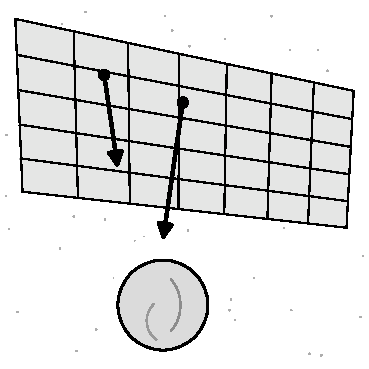
\includegraphics[width=0.72\textwidth]{fig_2.1.pdf}
\caption*{图 2.1\quad 全球性参考系的失效。由于每个粒子都感受到引力的影响，我们把"不加速"定义为"自由下落"。其后果是，无法再按照第1章概述的程序定义全球性的惯性坐标系，因为初始静止的粒子将开始相对这样一个参考系运动。}
\end{figure}

\begin{figure}[H]
\centering
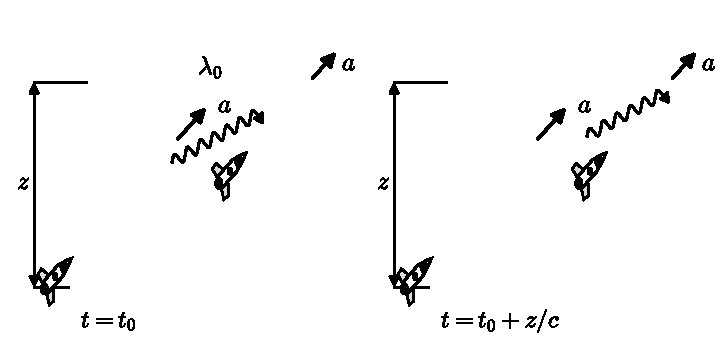
\includegraphics[width=0.72\textwidth]{fig_2.2.pdf}
\caption*{图 2.2\quad 由相距为$z$、各自感受加速度$a$的两个火箭测得的多普勒频移。}
\end{figure}

因此我们需要引入一种数学框架，使物理理论能够与这些结论相容。解决办法将是设想时空具有弯曲的几何，而引力是这种曲率的一种表现。用来描述曲率的恰当数学结构就是\emph{微分流形}（differentiable manifold）：本质上，它是一类局部看起来像平直空间、但整体几何可能非常不同的集合。（记住，EEP可以表述为“在时空的小区域中物理定律归结为狭义相对论的定律”，这与“局部类似于平直空间的集合”这一数学观念配合得很好。）

我们无法证明引力应当被看成时空的曲率；我们能做的是提出这个想法，推导它的种种后果，然后看结果是否与我们关于世界的经验合理地相符。让我们着手来做这件事。

考虑EEP最著名的预言之一：引力红移（gravitational redshift）。想象两个火箭相距为$z$，各自以某个恒定的加速度$a$在远离任何引力场的区域中运动，如图 2.2 所示。在时刻$t_0$，后方火箭发出一个波长为$\lambda_0$的光子。两火箭之间的距离保持不变，所以在我们的背景参考系中，光子经过时间$\Delta t = z/c$后到达前方火箭。（我们假设$\Delta v/c$很小，所以只算到一阶。）在这段时间里，火箭将获得附加速度$\Delta v = a\Delta t = az/c$。因此，到达前方火箭的光子将被通常的多普勒效应红移，红移量为
\begin{equation*}
\frac{\Delta\lambda}{\lambda_0} = \frac{\Delta v}{c} = \frac{az}{c^2}.
\tag{2.5}
\end{equation*}
按照EEP，同样的事情也应该发生在一个均匀引力场中。于是我们想象一座高度为$z$的塔矗立在某颗行星的表面上，引力场强度为$a_g$（也就是Newton所说的“重力加速度”），如图 2.3 所示。我们设想塔顶火箭中的观者能够探测到从地面发出的光子，但除此之外他们无法看到外面，从而不知道自己正坐在一座塔顶。换句话说，他们没有办法把这种情形与加速火箭的情形区分开。因此，EEP让我们能够立即得出结论：从地面发出的波长为$\lambda_0$的光子将被红移，红移量为
\begin{equation*}
\frac{\Delta\lambda}{\lambda_0} = \frac{a_g z}{c^2}.
\tag{2.6}
\end{equation*}
这就是著名的引力红移。注意，它是EEP的直接推论；并不需要广义相对论的细节。

\begin{figure}[H]
\centering
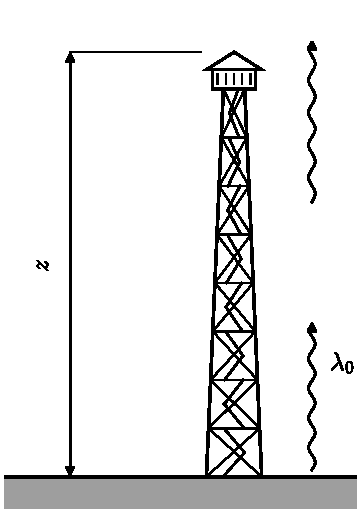
\includegraphics[width=0.72\textwidth]{fig_2.3.pdf}
\caption*{图 2.3\quad 地球表面上的引力红移，由不同高度的观者测量。}
\end{figure}

红移公式更常用Newton势$\Phi$来表述，其中$\mathbf{a}_g = \nabla\Phi$。（符号与通常的约定相反，因为我们这里把$\mathbf{a}_g$看成参考系的加速度，而不是粒子相对该参考系的加速度。）$\Phi$的非常数梯度类似于一个随时间变化的加速度，等价的净速度由对光子从发射到吸收之间的时间积分给出。于是我们有
\begin{align*}
\frac{\Delta\lambda}{\lambda_0} &= \frac{1}{c}\int \nabla\Phi\, dt\\
&= \frac{1}{c^2}\int \partial_z\Phi\, dz\\
&= \Delta\Phi,
\tag{2.7}
\end{align*}
其中$\Delta\Phi$是引力势的总变化，而且我们再一次令$c=1$。这个简单的引力红移公式在更普遍的情形下依然成立。当然，只要用到了Newton势，我们就把适用范围限制在了弱引力场。

我们已经从EEP出发论证了引力红移的存在；现在可以用这个现象来进一步支持“应当把时空看成弯曲的”这一观念。考虑与之前相同的实验装置，只是现在画在图 2.4 的时空图中。地面上的物理学家从高度$z_0$处发出一束波长为$\lambda_0$的光，光传播到高度为$z_1$的塔顶。从光的任意一个波长的起点被发出，到这同一个波长的终点被发出，二者之间的时间间隔是$\Delta t_0 = \lambda_0/c$；而吸收端相应的时间间隔是$\Delta t_1 = \lambda_1/c$，时间分别由位于两个高度处的时钟测量。既然我们设想引力场是静态的，单个波的波前与波尾所经过的时空路径就必须严格全等。（图中用一般的弯曲路径来表示它们，因为我们并不假装知道这些路径究竟是什么样子。）简单的几何似乎意味着$\Delta t_0$与$\Delta t_1$必定相同。但它们当然不相同；引力红移意味着高处的实验者每秒观测到的波长数目更少，所以$\Delta t_1 > \Delta t_0$。我们可以粗略地把这解释为“塔上的钟似乎走得更快”。那么，哪里出了问题？出在简单的几何上——光子所穿过的时空是弯曲的。

\begin{figure}[H]
\centering
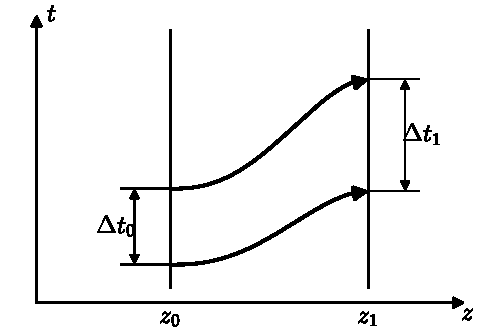
\includegraphics[width=0.72\textwidth]{fig_2.4.pdf}
\caption*{图 2.4\quad 图 2.3 所绘引力红移实验的时空图。不同时刻出发的时空路径是全等的，但地面与塔上测得的时间间隔不同，这标志着欧几里得几何的失效。}
\end{figure}

因此，我们希望把时空描述成这样一种数学结构：它在局部看起来像 Minkowski 空间，但在延展的区域上可能具有非平凡的曲率。涵盖这一观念的那类对象就是流形。在本章中，我们将只限于理解流形的概念以及可以在其上定义的各种结构，而把曲率的精确刻画留到下一章。

% 2.2 What Is a Manifold?
\section{什么是流形？}

流形（或微分流形）是数学和物理学中最基本的概念之一。我们都熟悉$n$维欧几里得空间$\mathbf{R}^n$的性质，它是$n$元组$(x^1,\ldots,x^n)$的集合，通常还配备一个平直的正定度规，其分量为$\delta_{ij}$。数学家们多年来致力于发展$\mathbf{R}^n$中的分析理论——微分、积分、函数的性质等等。但显然还存在其他一些空间（比如球面），我们直觉上认为它们是“弯曲的”，或者也许在拓扑上很复杂，我们也希望在它们上面进行类似的操作。

为了解决这个问题，我们发明了流形的概念，它对应于这样一种空间：可以是弯曲的，可以有复杂的拓扑，但在局部区域看起来就像$\mathbf{R}^n$。这里“看起来像”并不是说度规相同，而只是说一些更原初的概念——比如函数和坐标——以类似的方式运作。整个流形是通过把这些局部区域光滑地缝合在一起而构造出来的。一个关键的要点是，所使用的欧几里得空间的维数$n$在流形的每一片（patch）上都必须相同；这时我们就说这个流形的维数是$n$。用这种方法，我们可以通过把函数（局部地）转化为欧几里得空间中的函数，来分析这类空间上的函数。流形的例子包括：

\begin{itemize}
\item $\mathbf{R}^n$本身，包括直线（$\mathbf{R}$）、平面（$\mathbf{R}^2$）等等。这一点应当是显然的，因为$\mathbf{R}^n$不仅在局部而且在整体上都看起来像$\mathbf{R}^n$。
\item $n$维球面（$n$-sphere）$S^n$。它可以定义为$\mathbf{R}^{n+1}$中与原点相距某个固定距离的所有点的轨迹。圆周当然是$S^1$，而二维球面$S^2$是流形最有用的例子之一。（零维球面$S^0$，如果你仔细想想，由两个点组成。我们说$S^0$是一个不连通的零维流形。）值得强调的是，借助在$\mathbf{R}^{n+1}$中的嵌入来定义$S^n$只是一个方便的捷径；我们将讨论的所有流形都可以就其自身来定义，而无需求助于更高维的平直空间。
\item $n$维环面（$n$-torus）$T^n$，由取一个$n$维立方体并认同其相对的面而得到。二维环面$T^2$是一个认同了对边的正方形，如图 2.5 所示。甜甜圈的表面是一个大家熟悉的例子。
\item 亏格（genus）为$g$的黎曼面（Riemann surface），本质上是有$g$个洞而不止一个洞的二维环面，如图 2.6 所示。$S^2$可以看成亏格为零的黎曼面。用专业术语来说（这与我们眼下的讨论关系不大），每一个“紧致、可定向、无边界”的二维流形都是某个亏格的黎曼面。
\item 更抽象一些，由连续变换构成的集合，比如$\mathbf{R}^n$中的转动，构成一个流形。李群（Lie group）是同时还具有群结构的流形。例如SO(2)，即二维空间中转动的集合，就与$S^1$是同一个流形（尽管一般而言群流形会比球面更复杂）。
\item 两个流形的直积（direct product）是流形。也就是说，给定维数为$n$和$n'$的流形$M$和$M'$，我们可以构造一个维数为$n+n'$的流形$M\times M'$，它由有序对$(p,p')$组成，其中$p\in M$，$p'\in M'$。
\end{itemize}

\begin{figure}[H]
\centering
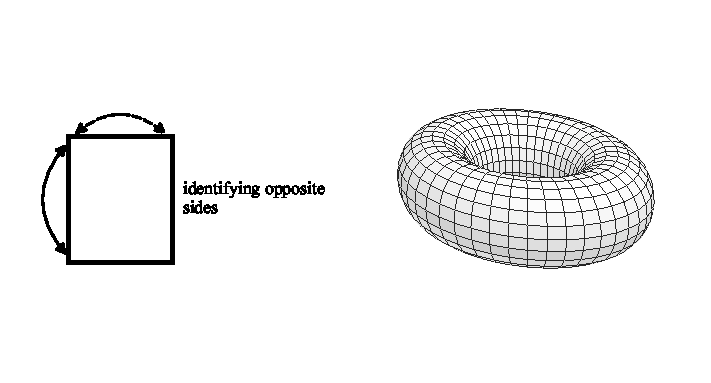
\includegraphics[width=0.72\textwidth]{fig_2.5.pdf}
\caption*{图 2.5\quad 通过认同正方形的对边构造出的环面$T^2$。}
\end{figure}

\begin{figure}[H]
\centering
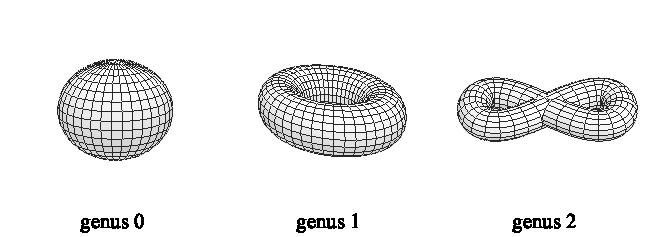
\includegraphics[width=0.72\textwidth]{fig_2.6.pdf}
\caption*{图 2.6\quad 不同亏格的黎曼面（genera是"genus"的复数）。}
\end{figure}

看了这么多例子，流形的概念可能显得空洞无物：哪些东西\emph{不是}流形呢？很多东西都不是流形，因为它们在某些地方局部看起来不像$\mathbf{R}^n$。例子包括：一条撞进二维平面里的一维直线，以及在顶点处粘在一起的两个锥面，如图 2.7 所示。更微妙的例子见图 2.8。比如考虑一个单独的（二维）锥面。显然，在某种意义上锥面局部看起来像$\mathbf{R}^2$；与此同时，同样明显的是，锥面的顶点处有某种奇异的东西。这正是“微分流形”中“可微”一词开始发挥作用的地方；正如我们在发展形式定义时将会看到的，作为流形，锥面是完全光滑的，尽管其曲率在顶点处并不光滑。（其他类型的奇异性更加严重，会使我们无法把某些空间看成流形——无论光滑与否。）另一个例子是线段（包括端点）。由于端点的存在，它肯定不符合我们将要发展的流形定义。尽管如此，我们可以把定义加以推广，把“带边流形”（manifolds with boundary）包括进来，线段就是它们的范例。关于带边流形的简要讨论见附录D。

\begin{figure}[H]
\centering
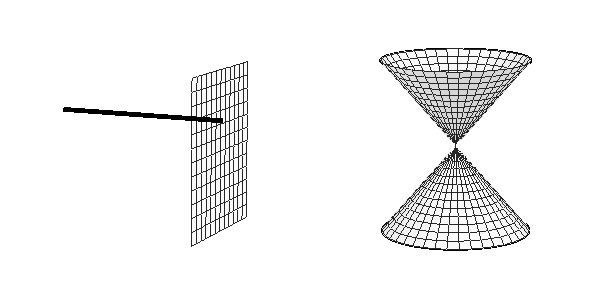
\includegraphics[width=0.72\textwidth]{fig_2.7.pdf}
\caption*{图 2.7\quad 不是流形的空间的例子：一条终止于平面上的直线，以及在顶点处相交的两个锥面。每种情形中都存在一个点，它在局部看起来不像固定维数的欧几里得空间。}
\end{figure}

\begin{figure}[H]
\centering
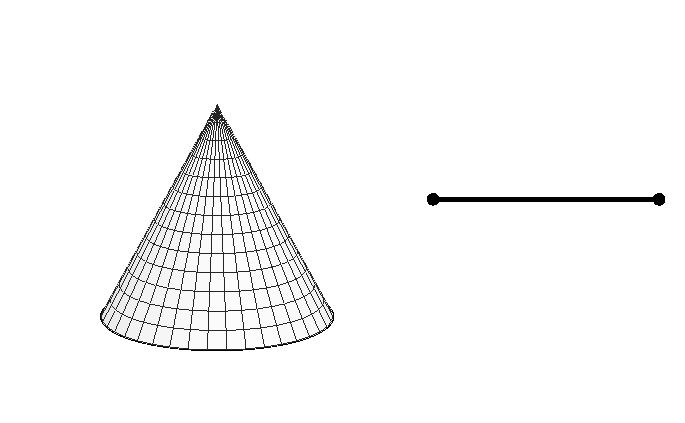
\includegraphics[width=0.72\textwidth]{fig_2.8.pdf}
\caption*{图 2.8\quad 微妙的例子。单个锥面是光滑流形，尽管其曲率在顶点处奇异。线段不是流形，但可以用更一般的"带边流形"概念来描述。}
\end{figure}

这些微妙的情形应该会让你相信，一个严格的定义是必要的，我们现在就开始构造它；这里的讨论遵循Wald (1984)的路数。流形的非正式想法是：一个由一些局部看起来像$\mathbf{R}^n$的“片”（patch）光滑地缝合而成的空间。因此我们需要把“局部看起来像$\mathbf{R}^n$”和“光滑地缝合在一起”这两个观念形式化。我们需要若干预备定义，其中大多数都相当明白，但完整一点总是好的。最基本的概念是两个集合之间的\textbf{映射}（map）。（我们假定你知道集合是什么，或者你认为你知道；我们不需要太精确。）给定两个集合$M$和$N$，映射$\phi:M\to N$是这样一种关系：它把$M$的每个元素恰好指派为$N$的一个元素。因此，映射不过是函数的简单推广。给定两个映射$\phi:A\to B$和$\psi:B\to C$，我们通过运算$(\psi\circ\phi)(a)=\psi(\phi(a))$定义\textbf{复合}（composition）$\psi\circ\phi:A\to C$，如图 2.9 所示。于是$a\in A$，$\phi(a)\in B$，从而$(\psi\circ\phi)(a)\in C$。映射书写的次序是有意义的，因为右边的先作用。

如果$N$的每个元素至多有一个$M$的元素被映入其中，就称映射$\phi$是\textbf{一一的}（one-to-one，或单射/injective）；如果$N$的每个元素至少有一个$M$的元素被映入其中，就称它是\textbf{映上的}（onto，或满射/surjective）。（想一想就会发现，“one-to-one”更好的名字应该是“one-from-one”，或者干脆叫“two-to-two”。）考虑函数$\phi:\mathbf{R}\to\mathbf{R}$。那么$\phi(x)=e^x$是一一的但不是映上的；$\phi(x)=x^3-x$是映上的但不是一一的；$\phi(x)=x^3$两者都是；而$\phi(x)=x^2$两者都不是，如图 2.10 所示。

\begin{figure}[H]
\centering
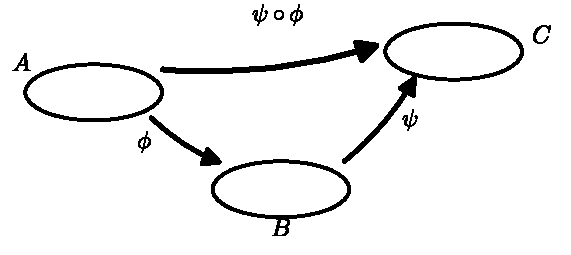
\includegraphics[width=0.72\textwidth]{fig_2.9.pdf}
\caption*{图 2.9\quad 映射$\psi\circ\phi:A\to C$由$\phi:A\to B$与$\psi:B\to C$复合而成。}
\end{figure}

\begin{figure}[H]
\centering
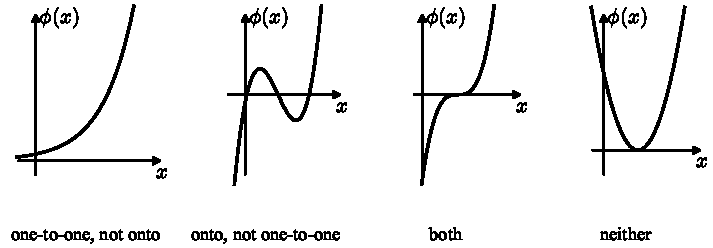
\includegraphics[width=0.72\textwidth]{fig_2.10.pdf}
\caption*{图 2.10\quad 几类映射。}
\end{figure}

集合$M$称为映射$\phi$的\textbf{定义域}（domain），$M$被映入的$N$中那些点的集合称为$\phi$的\textbf{像}（image）。对任何子集$U\subset N$，$M$中被映到$U$的元素的集合称为$U$在$\phi$下的\textbf{原像}（preimage），记作$\phi^{-1}(U)$。既一一又映上的映射称为\textbf{可逆的}（invertible，或双射/bijective）。这时我们可以定义\textbf{逆映射}（inverse map）$\phi^{-1}:N\to M$，它满足$(\phi^{-1}\circ\phi)(a)=a$，如图 2.11 所示。注意，同一个符号$\phi^{-1}$既用于原像也用于逆映射，尽管前者总是有定义，而后者只在某些特殊情形下才有定义。

\begin{figure}[H]
\centering
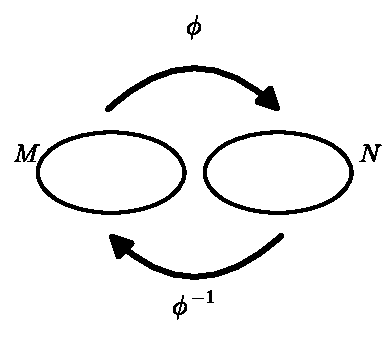
\includegraphics[width=0.72\textwidth]{fig_2.11.pdf}
\caption*{图 2.11\quad 一个映射及其逆映射。}
\end{figure}

映射的\textbf{连续性}（continuity）概念实际上是一个非常微妙的概念，其精确表述我们并不需要。我们将假定你理解连续性和可微性这两个概念对于通常的函数（即映射$\phi:\mathbf{R}\to\mathbf{R}$）的含义。接下来，把这些概念推广到更一般的欧几里得空间之间的映射$\phi:\mathbf{R}^m\to\mathbf{R}^n$将会很有用。从$\mathbf{R}^m$到$\mathbf{R}^n$的映射把一个$m$元组$(x^1,x^2,\ldots,x^m)$变成一个$n$元组$(y^1,y^2,\ldots,y^n)$，因此可以看成$n$个$m$元函数$\phi^i$的汇集：
\begin{equation*}
\begin{gathered}
y^1 = \phi^1(x^1, x^2, \ldots, x^m)\\
y^2 = \phi^2(x^1, x^2, \ldots, x^m)\\
y^n = \phi^n(x^1, x^2, \ldots, x^m).
\end{gathered}
\tag{2.8}
\end{equation*}
如果这些函数中的任何一个的$p$阶导数存在且连续，我们就称它为$C^p$的；如果$\phi:\mathbf{R}^m\to\mathbf{R}^n$的每个分量函数都至少是$C^p$的，我们就称整个映射为$C^p$的。于是，$C^0$映射连续但不一定可微，而$C^\infty$映射连续并且可以想微分多少次就微分多少次。例如考虑一元函数$\phi(x)=|x^3|$。这个函数除$x=0$外处处无穷可微，而在$x=0$处可微两次但不能三次；因此我们说它是$C^2$的。$C^\infty$映射有时称为\textbf{光滑}（smooth）。

如果存在一个$C^\infty$映射$\phi:M\to N$，其逆$\phi^{-1}:N\to M$也是$C^\infty$的，我们就称两个集合$M$和$N$是\textbf{微分同胚的}（diffeomorphic）；这时映射$\phi$就称为一个\textbf{微分同胚}（diffeomorphism）。这是我们关于“两个空间作为流形是相同的”所拥有的最好概念。例如，当我们说SO(2)与$S^1$是同一个流形时，意思就是它们微分同胚。更多的讨论见附录B。

这些基本定义你可能早已熟悉，哪怕只是记得个大概。现在我们将把它们用于流形的严格定义。遗憾的是，要把这个相对直观的概念形式化，需要一套多少有些繁复的程序。我们必须首先定义开集的概念，在开集上我们可以放置坐标系，然后再以恰当的方式把开集缝合起来。

我们从\textbf{开球}（open ball）的概念开始，它是$\mathbf{R}^n$中所有满足$|x-y|<r$的点$x$的集合，其中$y\in\mathbf{R}^n$和$r\in\mathbf{R}$固定，而$|x-y|=\left[\sum_i(x^i-y^i)^2\right]^{1/2}$。注意这是一个严格不等式——开球就是以$y$为中心、半径为$r$的$n$维球面的内部，如图 2.12 所示。$\mathbf{R}^n$中的\textbf{开集}（open set）是由开球的任意（可能是无限的）并构造出来的集合。换句话说，$V\subset\mathbf{R}^n$是开的，如果对任何$y\in V$，都存在一个以$y$为中心、完全位于$V$内部的开球。粗略地说，开集就是某个$(n-1)$维闭曲面的内部（或者若干个这种内部的并）。

\begin{figure}[H]
\centering
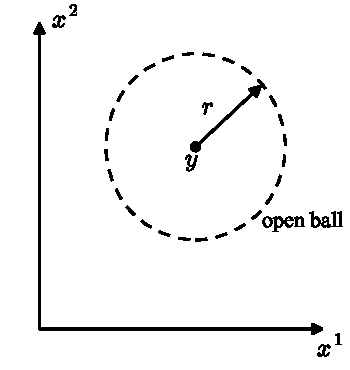
\includegraphics[width=0.72\textwidth]{fig_2.12.pdf}
\caption*{图 2.12\quad 定义在$\mathbf{R}^n$中的开球。}
\end{figure}

\textbf{卡片}（chart）或\textbf{坐标系}（coordinate system）由一个集合$M$的子集$U$连同某个一一映射$\phi:U\to\mathbf{R}^n$组成，且像$\phi(U)$在$\mathbf{R}^n$中是开的，如图 2.13 所示。（任何映射都是映到其像上的，所以只要$\phi:U\to\phi(U)$是一一的，它就可逆。）这样我们就可以说$U$是$M$中的一个开集。一个$C^\infty$的\textbf{图册}（atlas）是卡片的带指标的汇集$\{(U_\alpha,\phi_\alpha)\}$，它满足两个条件：
\begin{enumerate}
\item 各$U_\alpha$的并等于$M$；也就是说，诸$U_\alpha$覆盖$M$。
\item 各卡片光滑地缝合在一起。更精确地说，如果两张卡片重叠，$U_\alpha\cap U_\beta\neq\varnothing$，那么映射$(\phi_\alpha\circ\phi_\beta^{-1})$把$\phi_\beta(U_\alpha\cap U_\beta)\subset\mathbf{R}^n$中的点\emph{映上}到开集$\phi_\alpha(U_\alpha\cap U_\beta)\subset\mathbf{R}^n$，并且所有这些映射在其有定义之处必须是$C^\infty$的。参照图 2.14（改编自Wald (1984)）应当会更清楚。
\end{enumerate}
所以，卡片就是我们通常所想的某个开集上的坐标系，而图册就是在重叠处彼此光滑相容的一个卡片系统。

\begin{figure}[H]
\centering
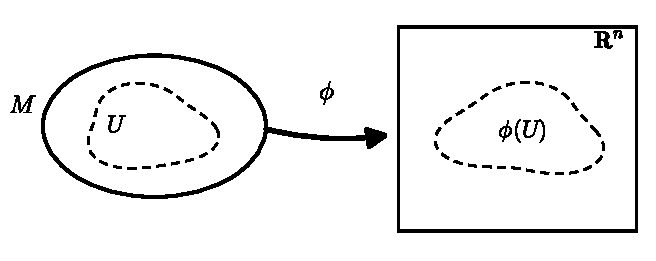
\includegraphics[width=0.72\textwidth]{fig_2.13.pdf}
\caption*{图 2.13\quad 覆盖$M$的开子集$U$的一个坐标卡片。}
\end{figure}

\begin{figure}[H]
\centering
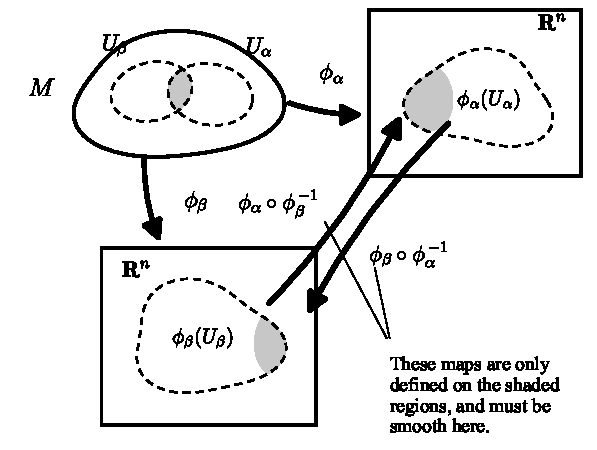
\includegraphics[width=0.72\textwidth]{fig_2.14.pdf}
\caption*{图 2.14\quad 相互重叠的坐标卡片。}
\end{figure}

于是，经过漫长的铺垫：一个$C^\infty$的$n$维\textbf{流形}（manifold，或简称$n$维流形）不过是一个集合$M$连同它的一个极大图册，即包含每一个可能的相容卡片的图册。在上述所有定义中，我们也可以把$C^\infty$换成$C^p$。对我们的目的来说，流形的可微程度并不关键；我们总是假定任何流形都具有当前应用所必需的可微性。要求图册是极大的，是为了让配备了不同图册的两个等价空间不被算作不同的流形。这个定义用形式化的语言捕捉了我们关于“局部看起来像$\mathbf{R}^n$的集合”的观念。当然，我们很少会需要用上这个定义的全部力量，但精确本身就是一种回报。

我们的这个定义有一个好处：它不依赖于把流形嵌入某个更高维的欧几里得空间。实际上，任何$n$维流形都可以嵌入$\mathbf{R}^{2n}$中（Whitney嵌入定理），有时我们也会用到这个事实，比如上面我们对球面的定义。（克莱因瓶就是一个二维流形的例子，它不能嵌入$\mathbf{R}^3$，尽管可以嵌入$\mathbf{R}^4$。）但重要的是要认识到，流形具有独立于任何嵌入的单独存在性。例如，我们没有必要相信四维时空是被塞在某个更大的空间里的。不过话说回来，它也可能是；我们真的不知道。弦论的近期进展使人提出这样的猜想：我们可见的宇宙其实也许是更高维空间中的一张“膜”（brane，“membrane”的推广）。但就经典GR而言，四维的图景完全够用。

为什么有必要在卡片及其重叠的问题上如此讲究，而不是干脆用一张卡片覆盖每一个流形？因为大多数流形无法只用一张卡片覆盖。考虑最简单的例子$S^1$。有一个常规的坐标系$\theta:S^1\to\mathbf{R}$，其中$\theta=0$取在圆周的顶部，绕一圈直到$2\pi$。然而，在卡片的定义中我们已经要求像$\theta(S^1)$在$\mathbf{R}$中是开的。如果取$\theta=0$或$\theta=2\pi$中的任何一个，我们得到的都是一个闭区间而不是开区间；如果两个点都不取，我们
% 本文件至此为止：书页60末句止于"如果两个点都不取，我们"，正文延续到书页61，由下一块接续。
 尚未覆盖整个圆。因此我们至少需要两个卡片，如图 2.15 所示。
\begin{figure}[H]
\centering
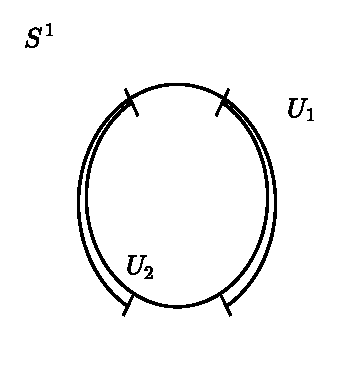
\includegraphics[width=0.72\textwidth]{fig_2.15.pdf}
\caption*{图 2.15\quad 共同覆盖 $S^1$ 的两个坐标卡片。}
\end{figure}
% ---- 书页 61 / p076 ----
一个稍微复杂些的例子由 $S^2$ 提供：同样，没有任何单个卡片能覆盖整个流形。绘制世界地图时传统上使用的墨卡托投影（Mercator projection）就同时漏掉了北极和南极（还有国际日期变更线（International Date Line），它涉及的角度 $\theta$ 的问题与我们在 $S^1$ 中发现的相同）。我们把 $S^2$ 取为 $\mathbf{R}^3$ 中由 $(x^1)^2+(x^2)^2+(x^3)^2=1$ 所定义的点集。我们可以从一个开集 $U_1$ 出发构造一个卡片，$U_1$ 定义为球面去掉北极之后的集合；构造方法是球极投影（stereographic projection），如图 2.16 所示。具体做法是：从北极向由 $x^3=-1$ 定义的平面画一条直线，给 $S^2$ 上被这条直线截住的点指定平面上相应点的笛卡尔坐标 $(y^1,y^2)$。明确写出来，这个映射就是
\begin{equation*}
\phi_1(x^1,x^2,x^3)\equiv(y^1,y^2)=\left(\frac{2x^1}{1-x^3}\,,\ \frac{2x^2}{1-x^3}\right). \tag{2.9}
\end{equation*}
请你自行验证这一点。另一个卡片 $(U_2,\phi_2)$ 则由从南极向 $x^3=+1$ 所定义的平面投影得到。所得坐标覆盖去掉南极的球面，具体为
\begin{equation*}
\phi_2(x^1,x^2,x^3)\equiv(z^1,z^2)=\left(\frac{2x^1}{1+x^3}\,,\ \frac{2x^2}{1+x^3}\right). \tag{2.10}
\end{equation*}
这两个卡片合起来覆盖了整个流形，而且它们在区域 $-1<x^3<+1$ 中相互交叠。你可以验证的另一件事是，复合映射 $\phi_2\circ\phi_1^{-1}$ 由下式给出
\begin{equation*}
z^i=\frac{4y^i}{\left[(y^1)^2+(y^2)^2\right]}, \tag{2.11}
\end{equation*}
\begin{figure}[H]
\centering
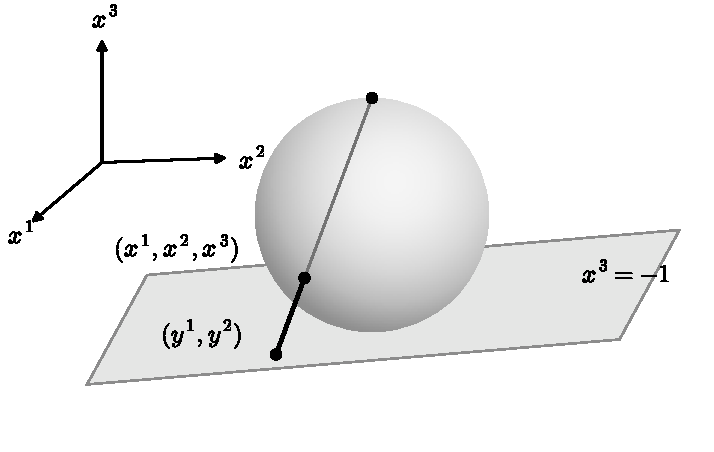
\includegraphics[width=0.72\textwidth]{fig_2.16.pdf}
\caption*{图 2.16\quad 通过从北极向切于南极的平面投影，在 $S^2$ 上定义球极坐标卡片。这样的卡片覆盖了除北极本身之外的整个球面。}
\end{figure}
% ---- 书页 62 / p077 ----
\begin{figure}[H]
\centering
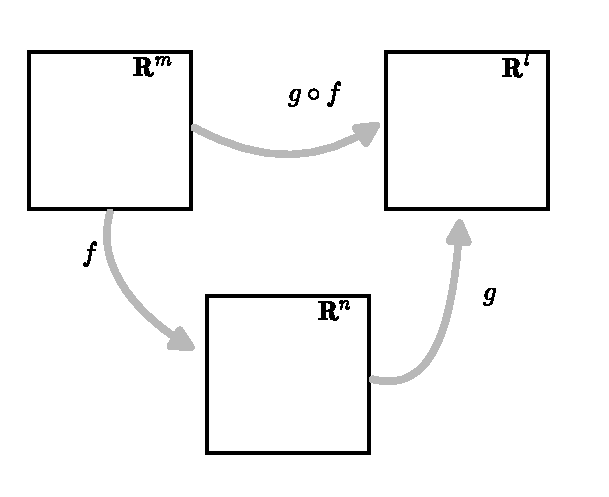
\includegraphics[width=0.72\textwidth]{fig_2.17.pdf}
\caption*{图 2.17\quad 链式法则把 $g\circ f$ 的偏导数与 $g$ 和 $f$ 各自的偏导数联系起来。}
\end{figure}
并且在交叠区域中是 $C^\infty$ 的。只要我们把注意力限制在这个区域，式 (2.11) 就正是我们通常所理解的坐标变换。

于是我们看到了卡片和图册的必要性：许多流形无法用单一的坐标系覆盖。尽管如此，用单个卡片来工作常常是方便的，只需随时记住没有被包含进去的那组点即可。

后面我们会用到的常规微积分中的一件武器是\textbf{链式法则}（chain rule）。设想我们有两个映射 $f:\mathbf{R}^m\to\mathbf{R}^n$ 和 $g:\mathbf{R}^n\to\mathbf{R}^l$，从而有复合映射 $(g\circ f):\mathbf{R}^m\to\mathbf{R}^l$，如图 2.17 所示。我们可以用分量来标记每个空间中的点：$\mathbf{R}^m$ 上用 $x^a$，$\mathbf{R}^n$ 上用 $y^b$，$\mathbf{R}^l$ 上用 $z^c$，指标各自取适当的取值范围。链式法则把复合映射的偏导数与各个映射的偏导数联系起来：
\begin{equation*}
\frac{\partial}{\partial x^a}(g\circ f)^c=\sum_b \frac{\partial f^b}{\partial x^a}\frac{\partial g^c}{\partial y^b}. \tag{2.12}
\end{equation*}
通常把它缩写为
\begin{equation*}
\frac{\partial}{\partial x^a}=\sum_b \frac{\partial y^b}{\partial x^a}\frac{\partial}{\partial y^b}. \tag{2.13}
\end{equation*}
使用这种简写形式的链式法则既不违法也不违背道德，但你应当能够在头脑中构想出这一构造背后的那些映射。回忆一下，当 $m=n$ 时，矩阵 $\partial y^b/\partial x^a$ 的行列式称为该映射的\textbf{雅可比行列式}（Jacobian），而且只要雅可比行列式非零，映射就可逆。

% ---- 书页 63 / p078 ----

\section{再谈矢量}

打好了这些基础，我们现在可以着手在流形上引入各种类型的结构了。我们从矢量与切空间（tangent space）开始。在讨论狭义相对论时，我们对矢量的定义以及矢量与时空的关系刻意含糊其辞。我们强调过的一点是切空间的概念——即时空中单个一点上所有矢量的集合。之所以如此强调，是为了从大家头脑中去除“矢量从流形上一个点拉伸到另一个点”的观念；矢量其实只是与单个点相联系的对象。采取这种观点暂时失去的，是理解诸如“矢量指向 $x$ 方向”这类说法的一条途径——如果切空间只是与每个点相联系的一个抽象矢量空间，就很难知道这类说法应当意味着什么。现在是解决这个问题的时候了。

设想我们想构造流形 $M$ 中一点 $p$ 处的切空间，而且只利用 $M$ 本身固有的东西（不嵌入更高维的空间）。第一反应也许是利用我们的直觉知识：存在一种叫做“曲线的切矢量”的对象，它们属于切空间。于是我们可能会考虑所有过 $p$ 点的参数化曲线的集合——也就是所有（非退化的）映射 $\gamma:\mathbf{R}\to M$ 构成的空间，要求 $p$ 属于 $\gamma$ 的像。一种诱人的做法是干脆把切空间定义为这些曲线在 $p$ 点的所有切矢量构成的空间。但这显然是作弊；切空间 $T_p$ 本应是 $p$ 点处矢量的空间，而在此之前，我们并没有“曲线的切矢量”应当是什么含义的独立概念。在某个坐标系 $x^\mu$ 中，任何过 $p$ 的曲线都通过 $n$ 个实数 $dx^\mu/d\lambda$（其中 $\lambda$ 是沿曲线的参量）确定了 $\mathbf{R}^n$ 中的一个元素，但这个映射明显依赖于坐标，而这并不是我们想要的。

不过我们的思路是对的，只是必须让一切不依赖于坐标。为此我们定义 $\mathcal{F}$ 为 $M$ 上全体光滑函数的空间（即 $C^\infty$ 映射 $f:M\to\mathbf{R}$）。然后我们注意到，每条过 $p$ 点的曲线都在这个空间上定义了一个算符——方向导数（directional derivative），它把 $f$ 映为 $df/d\lambda$（在 $p$ 点取值）。我们将给出如下论断：\emph{切空间 $T_p$ 可以等同于沿过 $p$ 点曲线的方向导数算符构成的空间}。为了确立这一想法，我们必须证明两件事：其一，方向导数构成的空间是一个矢量空间；其二，它正是我们想要的那种矢量空间（它与 $M$ 维数相同，能自然给出“指向某一方向的矢量”的概念，等等）。

第一个论断——方向导数构成矢量空间——看起来足够直接。设想两个算符 $d/d\lambda$ 与 $d/d\eta$，分别表示沿过 $p$ 点的两条曲线 $x^\mu(\lambda)$ 与 $x^\mu(\eta)$ 的导数。把它们相加并用实数缩放没有任何问题，于是得到新的算符 $a(d/d\lambda)+b(d/d\eta)$。然而，这个空间是否封闭并不一目了然；换句话说，所得的算符本身是否还是一个导数算符。一个好的导数算符应当线性地作用于函数，并且在函数的乘积上服从常规的 Leibniz（乘积）法则。我们的新算符显然是线性的，所以我们还需要
% ---- 书页 64 / p079 ----
验证它服从 Leibniz 法则。我们有
\begin{align*}
\left(a\frac{d}{d\lambda}+b\frac{d}{d\eta}\right)(fg)&=af\frac{dg}{d\lambda}+ag\frac{df}{d\lambda}+bf\frac{dg}{d\eta}+bg\frac{df}{d\eta}\\
&=\left(a\frac{df}{d\lambda}+b\frac{df}{d\eta}\right)g+\left(a\frac{dg}{d\lambda}+b\frac{dg}{d\eta}\right)f. \tag{2.14}
\end{align*}
\begin{figure}[H]
\centering
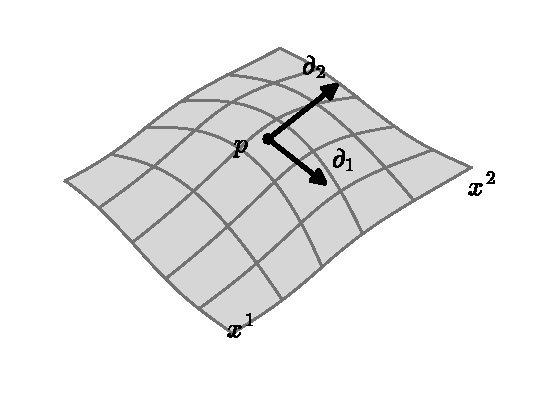
\includegraphics[width=0.72\textwidth]{fig_2.18.pdf}
\caption*{图 2.18\quad 偏导数定义为沿“保持所有其他坐标不变”的曲线的方向导数。}
\end{figure}
正如我们所希望的，乘积法则得到了满足，因此方向导数的集合是一个矢量空间。

它就是我们想要等同于切空间的那种矢量空间吗？让自己信服的最容易的办法，是为这个空间找一组基。再次考虑带有坐标 $x^\mu$ 的一个坐标卡片。于是在 $p$ 点有一组显而易见的 $n$ 个方向导数，即 $p$ 点的偏导数 $\partial_\mu$，如图 2.18 所示。注意，这其实就是对 $x^\mu$ 的偏导数的\emph{定义}：沿由“$x^\nu=$ 常数（对一切 $\nu\neq\mu$）”所定义、以 $x^\mu$ 本身为参量的曲线的方向导数。我们现在要宣称：$p$ 点的偏导数算符 $\{\partial_\mu\}$ 构成切空间 $T_p$ 的一组基。（由此立即可知 $T_p$ 是 $n$ 维的，因为基矢就这么多。）为了看到这一点，我们将证明任何方向导数都可以分解为实数与偏导数乘积之和。这正是大家熟悉的切矢量分量的表达式，不过能从这套“大机器”方法中看到它，也是件令人愉快的事。考虑一个 $n$ 维流形 $M$、一个坐标卡片 $\phi:M\to\mathbf{R}^n$、一条曲线 $\gamma:\mathbf{R}\to M$，以及一个函数 $f:M\to\mathbf{R}$。这就导致了图 2.19 所示的那一团相互纠缠的映射。如果 $\lambda$ 是沿 $\gamma$ 的参量，我们想把矢量/算符 $d/d\lambda$ 用偏导数 $\partial_\mu$ 表示出来。利用链式法则 (2.12)，我们有
% ---- 书页 65 / p080 ----
\begin{align*}
\frac{d}{d\lambda}f&=\frac{d}{d\lambda}(f\circ\gamma)\\
&=\frac{d}{d\lambda}\left[(f\circ\phi^{-1})\circ(\phi\circ\gamma)\right]\\
&=\frac{d(\phi\circ\gamma)^\mu}{d\lambda}\frac{\partial(f\circ\phi^{-1})}{\partial x^\mu}\\
&=\frac{dx^\mu}{d\lambda}\partial_\mu f. \tag{2.15}
\end{align*}
\begin{figure}[H]
\centering
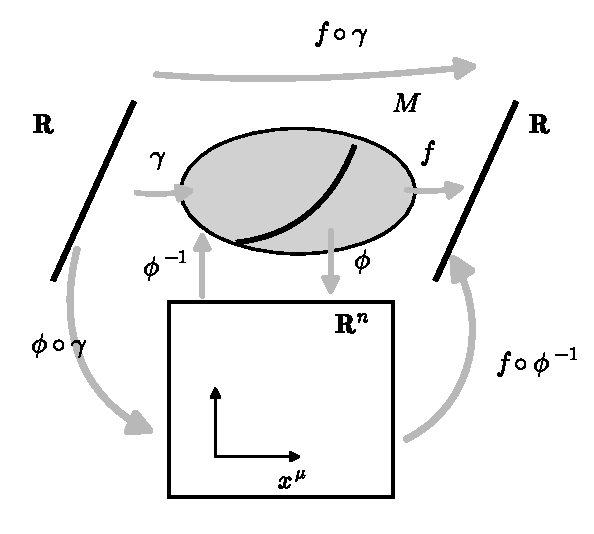
\includegraphics[width=0.72\textwidth]{fig_2.19.pdf}
\caption*{图 2.19\quad 把曲线 $\gamma:\mathbf{R}\to M$ 的切矢量按 $M$ 上坐标的偏导数分解。}
\end{figure}
第一行只是把左边的非正式表达式改写成函数 $(f\circ\gamma):\mathbf{R}\to\mathbf{R}$ 的实实在在的导数。第二行不过来自逆映射 $\phi^{-1}$ 的定义（以及复合运算的结合律）。第三行是正式的链式法则 (2.12)，最后一行则回到了开头的非正式记号。由于函数 $f$ 是任意的，我们有
\begin{equation*}
\frac{d}{d\lambda}=\frac{dx^\mu}{d\lambda}\partial_\mu. \tag{2.16}
\end{equation*}
这样，偏导数 $\{\partial_\mu\}$ 的确构成了方向导数矢量空间的一组好的基，因此我们可以放心地把它等同于切空间。

当然，$d/d\lambda$ 所代表的矢量是我们早已认识的；它就是以 $\lambda$ 为参量的曲线的切矢量。因此式 (2.16) 可以看作式 (1.38) 的重述，在那里我们曾宣称切矢量的分量就是 $dx^\mu/d\lambda$。唯一的区别在于，我们现在是在任意流形上工作，并且我们把基矢指定为 $\hat{e}_{(\mu)}=\partial_\mu$。

这种特殊的基（$\hat{e}_{(\mu)}=\partial_\mu$）称为 $T_p$ 的\textbf{坐标基}（coordinate basis）；它是“让基矢沿坐标轴指向”这一观念的形式化。考虑切矢量时，我们并没有理由只限于坐标基。例如，坐标基矢一般并不归一化到单位长度，彼此也不一定正交，我们很快就会看到
% ---- 书页 66 / p081 ----
这一点。这种局面可不是靠定义就能打发掉的；在弯曲流形上，只要某点处曲率不为零，坐标基在该点的任何邻域内都\emph{绝不会}是正交归一（orthonormal）的。当然，我们可以定义非坐标的正交归一基，例如在坐标基中给出它们的分量，有时这种技巧是有用的。然而，坐标基非常简单而自然，全书我们几乎只使用坐标基；想见识正交归一基，可参见附录 J。（在三维欧几里得空间的矢量分析研究中，标准做法是选取正交归一基而不是坐标基；因此，把 GR 教材中的公式应用到平直空间中非笛卡尔坐标的研究时，你应当多加小心。）

我们对矢量采取的这一颇为抽象的观点，其优点之一是：坐标变换下的变换规律立即可得。既然基矢是 $\hat{e}_{(\mu)}=\partial_\mu$，某个新坐标系 $x^{\mu'}$ 中的基矢就由链式法则 (2.13) 给出为
\begin{equation*}
\partial_{\mu'}=\frac{\partial x^\mu}{\partial x^{\mu'}}\partial_\mu. \tag{2.17}
\end{equation*}
我们可以用平直空间中使用过的同一技巧得到矢量分量的变换规律：要求矢量 $V=V^\mu\partial_\mu$ 在基的改变下不变。我们有
\begin{align*}
V^\mu\partial_\mu&=V^{\mu'}\partial_{\mu'}\\
&=V^{\mu'}\frac{\partial x^\mu}{\partial x^{\mu'}}\partial_\mu, \tag{2.18}
\end{align*}
于是，由于矩阵 $\partial x^{\mu'}/\partial x^\mu$ 是矩阵 $\partial x^\mu/\partial x^{\mu'}$ 的逆，
\begin{equation*}
V^{\mu'}=\frac{\partial x^{\mu'}}{\partial x^\mu}V^\mu. \tag{2.19}
\end{equation*}
由于基矢通常并不显式写出，分量变换规则 (2.19) 就是我们所说的“矢量变换定律”。我们注意到，它与狭义相对论中矢量分量在洛伦兹变换 $V^{\mu'}=\Lambda^{\mu'}{}_\nu V^\nu$ 下的变换是相容的，因为洛伦兹变换是一种特殊的坐标变换，即 $x^{\mu'}=\Lambda^{\mu'}{}_\nu x^\nu$。但 (2.19) 要普遍得多，它涵盖了矢量在任意坐标（从而基）改变下的行为，而不只是线性变换。一如既往，我们想强调的是一种有些微妙的存在论上的区分——原则上，张量分量在我们改变坐标时并不需要改变；它们是在我们改变切空间中的基时才改变的，只不过我们决定用坐标来定义基。因此，坐标的改变会诱发基的改变，如图 2.20 所示。

既然一点的矢量可以看成沿过该点的路径的方向导数算符，那么显然，矢量\emph{场}（vector field）定义了一个从光滑函数到光滑函数、遍布整个流形的映射，办法是在每一点取导数。给定两个矢量场 $X$ 和 $Y$，我们因此可以定义它们的\textbf{对易子}（commutator）$[X,Y]$，办法是由它作用在函数 $f(x^\mu)$ 上的效果来刻画：
% ---- 书页 67 / p082 ----
\begin{figure}[H]
\centering
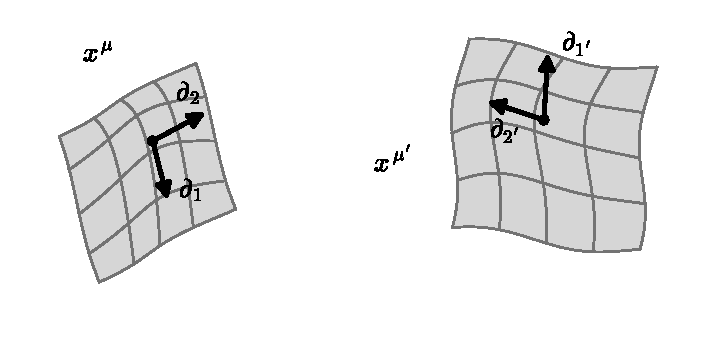
\includegraphics[width=0.72\textwidth]{fig_2.20.pdf}
\caption*{图 2.20\quad 坐标变换 $x^\mu\to x^{\mu'}$ 诱发切空间中基的改变。}
\end{figure}
\begin{equation*}
[X,Y](f)\equiv X(Y(f))-Y(X(f)). \tag{2.20}
\end{equation*}
抽象观点的好处在于，这个算符显然不依赖于坐标。事实上，两个矢量场的对易子本身还是一个矢量场：如果 $f$ 和 $g$ 是函数，$a$ 和 $b$ 是实数，则对易子是线性的，
\begin{equation*}
[X,Y](af+bg)=a[X,Y](f)+b[X,Y](g), \tag{2.21}
\end{equation*}
并且服从 Leibniz 法则，
\begin{equation*}
[X,Y](fg)=f[X,Y](g)+g[X,Y](f). \tag{2.22}
\end{equation*}
这两个性质都很容易验证，是颇有用处的练习。同样有趣的练习是推导矢量场 $[X,Y]^\mu$ 分量的显式表达式，结果是
\begin{equation*}
\boxed{[X,Y]^\mu=X^\lambda\partial_\lambda Y^\mu-Y^\lambda\partial_\lambda X^\mu}. \tag{2.23}
\end{equation*}
按构造这是一个良定义的张量；但你对其中偏导数的出现应当有一丝担忧，因为矢量的偏导数并不是良定义的张量（下一节我们会讨论这一点）。还有一项迷人的练习是对式 (2.23) 显式地做一次坐标变换，验证所有可能非张量化的部分都相互抵消，结果像一个矢量场那样变换。对易子是李导数（Lie derivative）的特例，李导数将在附录 B 中讨论；它有时也被称为\textbf{李括号}（Lie bracket）。注意，由于偏导数相互对易，由坐标函数的偏导数给出的矢量场 $\{\partial_\mu\}$ 的对易子永远为零。

% ---- 书页 68 / p083 ----
\section{再谈张量}

探索完矢量的世界，我们继续沿着在平直空间中走过的脚步前行，现在来考虑对偶矢量（one-form，1-形式）。余切空间 $T_p^*$ 同样可以看成线性映射 $\omega:T_p\to\mathbf{R}$ 的集合。1-形式最典型的例子是函数 $f$ 的梯度，记作 $\mathrm{d}f$，如式 (1.52) 那样。它作用在矢量 $d/d\lambda$ 上的结果，恰恰就是这个函数的方向导数：
\begin{equation*}
\mathrm{d}f\left(\frac{d}{d\lambda}\right)=\frac{df}{d\lambda}. \tag{2.24}
\end{equation*}
一个诱人的问题是：“为什么不能干脆把函数 $f$ 本身当作这个 1-形式，而把 $df/d\lambda$ 当作它的作用？”关键在于，1-形式和矢量一样，只存在于它被定义的那一点，不依赖于 $M$ 上其他点的信息。如果你知道一个函数在某点某个邻域内的取值，你可以求它的导数，但仅知道它在该点的值是不够的；而梯度恰恰编码了沿过 $p$ 点的任何曲线取方向导数所需的全部信息，从而尽到了它作为对偶矢量的职责。

你可能已经注意到，我们利用流形固有的结构（沿曲线的方向导数）定义了矢量，再用这个定义、借助对偶矢量空间来定义 1-形式。这或许会给人一个印象：矢量在某种意义上更基本。然而事实上，我们同样可以从 1-形式的内禀定义出发，再用它把矢量定义为对偶空间。粗略地说，$p$ 点的 1-形式空间等价于所有在 $p$ 点为零、且具有相同二阶偏导数的函数构成的空间。而且真要说起来，那样做反而更基本，因为我们可以给出所有 $q$-形式（具有 $q$ 个下指标的完全反对称张量）的内禀定义，我们将在 2.9 节讨论它们（尽管不会深入内禀定义的细节）。

正如沿坐标轴的偏导数为切空间提供了一组自然的基，坐标函数 $x^\mu$ 的梯度也为余切空间提供了一组自然的基。回忆一下，在平直空间中我们通过要求 $\hat{\theta}^{(\mu)}(\hat{e}_{(\nu)})=\delta^\mu_\nu$ 来构造 $T_p^*$ 的基。在任意流形上贯彻同样的思想，我们发现 (2.24) 导致
\begin{equation*}
\mathrm{d}x^\mu(\partial_\nu)=\frac{\partial x^\mu}{\partial x^\nu}=\delta^\mu_\nu. \tag{2.25}
\end{equation*}
因此，梯度 $\{\mathrm{d}x^\mu\}$ 是一组适当的基 1-形式；任意 1-形式按分量展开为 $\omega=\omega_\mu\mathrm{d}x^\mu$。

基对偶矢量与分量的变换性质，可以按如今已是家常便饭的步骤得到。对基 1-形式，我们得到
\begin{equation*}
\mathrm{d}x^{\mu'}=\frac{\partial x^{\mu'}}{\partial x^\mu}\mathrm{d}x^\mu \tag{2.26}
\end{equation*}
% ---- 书页 69 / p084 ----
而对分量则有
\begin{equation*}
\omega_{\mu'}=\frac{\partial x^\mu}{\partial x^{\mu'}}\omega_\mu. \tag{2.27}
\end{equation*}
以后谈到 1-形式 $\omega$ 时，我们通常直接写它的分量 $\omega_\mu$。

和平直空间中一样，$(k,l)$ 型张量是从 $k$ 个对偶矢量与 $l$ 个矢量组成的集合到 $\mathbf{R}$ 的多重线性映射。它在坐标基下的分量，可以让这个张量作用于基 1-形式和基矢而得到：
\begin{equation*}
T^{\mu_1\cdots\mu_k}{}_{\nu_1\cdots\nu_l}=T(\mathrm{d}x^{\mu_1},\ldots,\mathrm{d}x^{\mu_k},\partial_{\nu_1},\ldots,\partial_{\nu_l}). \tag{2.28}
\end{equation*}
这等价于展开式
\begin{equation*}
T=T^{\mu_1\cdots\mu_k}{}_{\nu_1\cdots\nu_l}\,\partial_{\mu_1}\otimes\cdots\otimes\partial_{\mu_k}\otimes\mathrm{d}x^{\nu_1}\otimes\cdots\otimes\mathrm{d}x^{\nu_l}. \tag{2.29}
\end{equation*}
一般张量的变换定律遵循同样的模式：把平直空间中使用的洛伦兹变换矩阵，换成代表更一般坐标变换的矩阵：
\begin{equation*}
\boxed{T^{\mu_1'\cdots\mu_k'}{}_{\nu_1'\cdots\nu_l'}=\frac{\partial x^{\mu_1'}}{\partial x^{\mu_1}}\cdots\frac{\partial x^{\mu_k'}}{\partial x^{\mu_k}}\frac{\partial x^{\nu_1}}{\partial x^{\nu_1'}}\cdots\frac{\partial x^{\nu_l}}{\partial x^{\nu_l'}}\,T^{\mu_1\cdots\mu_k}{}_{\nu_1\cdots\nu_l}.} \tag{2.30}
\end{equation*}
这个张量变换定律好记得很：只要看看指标的摆放位置，它实在不可能是别的样子。

不过实际上，变换张量时往往更省事的做法是：按字面接受“基矢就是偏导数、基 1-形式就是梯度”这一等式，然后直接把坐标变换代进去。举个例子，考虑二维流形上一个对称的 $(0,2)$ 型张量 $S$，它在坐标系 $(x^1=x,\ x^2=y)$ 下的分量为
\begin{equation*}
S_{\mu\nu}=\begin{pmatrix} 1 & 0 \\ 0 & x^2 \end{pmatrix}. \tag{2.31}
\end{equation*}
这可以等价地写成
\begin{align*}
S&=S_{\mu\nu}(\mathrm{d}x^\mu\otimes\mathrm{d}x^\nu)\\
&=(\mathrm{d}x)^2+x^2(\mathrm{d}y)^2, \tag{2.32}
\end{align*}
其中最后一行为了简洁省略了张量积符号（今后我们都将如此）。现在考虑新坐标
\begin{align*}
x'&=\frac{2x}{y}\\
y'&=\frac{y}{2} \tag{2.33}
\end{align*}
% ---- 书页 70 / p085 ----
（例如在 $x>0$、$y>0$ 时有效）。它们可以立即反解出来，得到
\begin{align*}
x&=x'y'\\
y&=2y'. \tag{2.34}
\end{align*}
我们不必动用张量变换定律，而只需利用我们知道如何求导这一事实，把 $\mathrm{d}x^\mu$ 用 $\mathrm{d}x^{\mu'}$ 表示出来。我们有
\begin{align*}
\mathrm{d}x&=y'\mathrm{d}x'+x'\mathrm{d}y'\\
\mathrm{d}y&=2\,\mathrm{d}y'. \tag{2.35}
\end{align*}
只需把这些表达式直接代入 (2.32)，就得到（记住张量积不对易，故 $\mathrm{d}x'\mathrm{d}y'\neq\mathrm{d}y'\mathrm{d}x'$）：
\begin{equation*}
S=(y')^2(\mathrm{d}x')^2+x'y'\left(\mathrm{d}x'\mathrm{d}y'+\mathrm{d}y'\mathrm{d}x'\right)+\left[(x')^2+4(x'y')^2\right](\mathrm{d}y')^2, \tag{2.36}
\end{equation*}
或者
\begin{equation*}
S_{\mu'\nu'}=\begin{pmatrix} (y')^2 & x'y' \\ x'y' & (x')^2+4(x'y')^2 \end{pmatrix}. \tag{2.37}
\end{equation*}
注意它仍然是对称的。我们没有直接使用变换定律 (2.30)，但如果直接用，也会得到相同的结果，你可以自行核验。

大体而言，我们在平直空间中定义的各种张量运算在更一般的场合依然如故：缩并、对称化，等等。但有三个重要的例外：偏导数、度规，以及 Levi-Civita 张量。我们先来看偏导数。

遗憾的是，张量的偏导数一般不是新的张量。标量的偏导数——梯度——如我们所见是名副其实的 $(0,1)$ 型张量。但更高阶张量的偏导数就不是张量性的了；只要考察 1-形式的偏导数 $\partial_\mu W_\nu$ 并变换到一个新坐标系，就能看到这一点：
\begin{align*}
\frac{\partial}{\partial x^{\mu'}}W_\nu&=\frac{\partial x^\mu}{\partial x^{\mu'}}\frac{\partial}{\partial x^\mu}\left(\frac{\partial x^\nu}{\partial x^{\nu'}}W_\nu\right)\\
&=\frac{\partial x^\mu}{\partial x^{\mu'}}\frac{\partial x^\nu}{\partial x^{\nu'}}\left(\frac{\partial}{\partial x^\mu}W_\nu\right)+W_\nu\frac{\partial x^\mu}{\partial x^{\mu'}}\frac{\partial}{\partial x^\nu}\frac{\partial x^\nu}{\partial x^{\nu'}}. \tag{2.38}
\end{align*}
假如 $\partial_\mu W_\nu$ 像 $(0,2)$ 型张量那样变换，最后一行中的第二项就不应该存在。可以看到，它之所以出现，是因为变换矩阵的导数不再为零——而在平直空间的洛伦兹变换下它原是为零的。

微分显然是物理学中的重要工具，所以我们将不得不发明新的张量化运算来接替偏导数。实际上我们会发明好几种：外微分（exterior derivative）、协变导数（covariant derivative）和李导数（Lie derivative）。

% ---- 书页 71 / p086 ----
\section{度规}

度规张量在弯曲空间中的地位如此重要，以至于它被赋予了一个新符号 $g_{\mu\nu}$（而 $\eta_{\mu\nu}$ 则专门保留给 Minkowski 度规）。对 $g_{\mu\nu}$ 分量的限制很少，只要求它是对称的 $(0,2)$ 型张量。通常——尽管并非总是——还要求它是非退化的（nondegenerate），意思是行列式 $g=|g_{\mu\nu}|$ 不为零。这使我们能够经由
\begin{equation*}
g^{\mu\nu}g_{\nu\sigma}=g_{\sigma\lambda}g^{\lambda\mu}=\delta^\mu_\sigma. \tag{2.39}
\end{equation*}
来定义逆度规 $g^{\mu\nu}$。

$g_{\mu\nu}$ 的对称性意味着 $g^{\mu\nu}$ 也是对称的。正如狭义相对论中那样，度规及其逆可用来升降张量的指标。你可能熟悉拓扑学研究中“度规”（metric）的概念，在那里还要求度规是正定的（没有负本征值）。广义相对论中使用的度规不能用来定义拓扑，但它会有其他用途。

要充分领略度规的全部荣耀尚需一些时间，但出于激励的目的[仿照 Sachs and Wu (1977)]，我们可以列出 $g_{\mu\nu}$ 将要承担的种种任务：（1）度规提供“过去”与“未来”的概念；（2）度规使计算路径长度和固有时成为可能；（3）度规确定两点之间的“最短距离”，从而确定检验粒子的运动；（4）度规取代 Newton 引力场 $\phi$；（5）度规提供局部惯性系的观念，从而给出“无转动”的意义；（6）度规通过定义光速——任何信号都无法超越的速度——来确定因果性；（7）度规取代 Newton 力学中传统的欧几里得三维点积。显然，这些想法并非都完全相互独立，但我们已经能对这个张量的重要性略窥一二。

在狭义相对论中讨论路径长度时，我们（有些含糊其辞地）引入了线元 $ds^2=\eta_{\mu\nu}\mathrm{d}x^\mu\mathrm{d}x^\nu$，用它来求路径的长度。当然，既然我们如今知道 $\mathrm{d}x^\mu$ 其实是一个基对偶矢，把“度规”和“线元”这两个词互换使用就变得自然而然了，于是写作
\begin{equation*}
ds^2=g_{\mu\nu}\,\mathrm{d}x^\mu\,\mathrm{d}x^\nu. \tag{2.40}
\end{equation*}
要做到完全一致，我们应当把它写作“$g$”，有时也确实如此；但更多时候 $g$ 被用来表示行列式 $|g_{\mu\nu}|$。例如我们知道，具有笛卡尔坐标的三维空间中，欧几里得线元为
\begin{equation*}
ds^2=(\mathrm{d}x)^2+(\mathrm{d}y)^2+(\mathrm{d}z)^2. \tag{2.41}
\end{equation*}
现在我们可以换到任何我们想用的坐标系。例如，取球坐标就有
% ---- 书页 72 / p087 ----
\begin{align*}
x&=r\sin\theta\cos\phi\\
y&=r\sin\theta\sin\phi\\
z&=r\cos\theta, \tag{2.42}
\end{align*}
这直接给出
\begin{equation*}
ds^2=\mathrm{d}r^2+r^2\,\mathrm{d}\theta^2+r^2\sin^2\theta\,\mathrm{d}\phi^2. \tag{2.43}
\end{equation*}
显然，度规的分量看上去与笛卡尔坐标下的不同，但空间的全部性质依然未变。

大多数文献不至于挑剔到要区分“$dx$”（无穷小位移的非正式概念）与“$\mathrm{d}x$”（严格的基 1-形式概念，由坐标函数的梯度给出）的地步。（它们还往往忽视张量积不对易这一事实，把诸如 $\mathrm{d}x\,\mathrm{d}y+\mathrm{d}y\,\mathrm{d}x$ 的表达式写成 $2\,\mathrm{d}x\,\mathrm{d}y$；含义如何应当能从上下文看清楚。）实际上，我们的记号“$ds^2$”既不指任何东西的微分，也不指任何东西的平方；它只是度规张量的习惯性简写，而度规张量是从两个矢量到实数的多重线性映射。于是，对两个矢量 $V^\mu$ 和 $W^\nu$ 的内积，我们有一组等价的表达式：
\begin{equation*}
g_{\mu\nu}V^\mu W^\nu=g(V,W)=ds^2(V,W). \tag{2.44}
\end{equation*}
而“$(\mathrm{d}x)^2$”则专门指实实在在的 $(0,2)$ 型张量 $\mathrm{d}x\otimes\mathrm{d}x$。

非欧流形的一个好例子是二维球面（two-sphere），它可以看成 $\mathbf{R}^3$ 中与原点距离为 1 的点的轨迹。$(\theta,\phi)$ 坐标系下的度规，可以在 (2.43) 中令 $r=1$ 和 $\mathrm{d}r=0$ 得到：
\begin{equation*}
ds^2=\mathrm{d}\theta^2+\sin^2\theta\,\mathrm{d}\phi^2. \tag{2.45}
\end{equation*}
这与把 $ds$ 解释为无穷小长度完全一致，如图 2.21 所示。任何用心读到这里的人都应当在此发问：“令 $\mathrm{d}r=0$ 到底是什么意思？我们知道 $\mathrm{d}r$ 是一个良定义的、非零的 1-形式场啊。”正如偶尔会发生的那样，我们这里用了不太严谨的语言，来引导一步实际上完全正当的操作；关于子流形如何从其所嵌入的空间继承度规，参见附录 A 中的讨论。

我们将会看到，度规张量包含了描述流形曲率所需的全部信息（至少在所谓的黎曼几何（Riemannian geometry）中是如此；下一章我们会讨论其中的若干微妙之处）。在 Minkowski 空间中，我们可以选取使度规分量为常数的坐标；但应当清楚，曲率是否存在这件事比“度规是否依赖于坐标”更为微妙，因为在上面的例子中我们已经看到，平直欧几里得空间在球坐标下的度规就是 $r$ 和 $\theta$ 的函数。后面我们将看到，度规分量为常数足以保证空间是平直的，而且事实上在任何
 平直空间上总存在一个度规分量为常数的坐标系。

\begin{figure}[H]
\centering
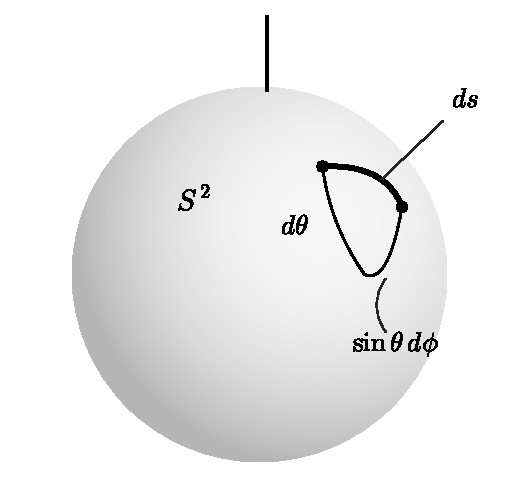
\includegraphics[width=0.72\textwidth]{fig_2.21.pdf}
\caption*{图 2.21\quad 二维球面上的线元。}
\end{figure}
% ---- 书页 73 / p088 ----
但是，我们未必知道如何找到这样一个坐标系，而且空间偏离平直的方式有很多种；因此我们会想要一个对曲率更精确的刻画，这将在后面引入。

把$g_{\mu\nu}$化成它的\textbf{规范形式}（canonical form），便得到度规的一个有用刻画。在这种形式下，度规分量变为
\begin{equation*}
g_{\mu\nu}=\mathrm{diag}\,(-1,-1,\ldots,-1,+1,+1,\ldots,+1,0,0,\ldots,0),
\tag{2.46}
\end{equation*}
其中“diag”指具有所给元素的对角矩阵。度规的\textbf{号差}（signature）指正、负本征值两者的个数；例如，对 Minkowski 空间我们会说“号差为负正正正的度规”。如果本征值中有零，度规就是“退化的”（degenerate），逆度规将不存在；如果度规连续且非退化，它的号差在每一点都相同。我们要处理的将总是连续、非退化的度规。如果所有符号都是正的，这个度规就称为\textbf{欧几里得型}（Euclidean）或\textbf{黎曼型}（Riemannian）的（或者干脆叫\textbf{正定}（positive definite）的）；如果只有单独一个负号，则称为\textbf{洛伦兹型}（Lorentzian）或\textbf{伪黎曼型}（pseudo-Riemannian）的；而任何既有若干$+1$又有若干$-1$的度规都称为\textbf{不定}（indefinite）的。（于是，“欧几里得”一词有时意味着空间是平直的，有时又不是，但它始终意味着规范形式严格为正；这套术语令人遗憾，却是通行的标准。）广义相对论中感兴趣的时空都具有洛伦兹型度规。

我们还没有证明总可以把度规化成规范形式。事实上，在$M$的某一点$p$处总能做到这一点，但一般而言只在单独那一点处可行，在$p$的任何邻域内则不然。实际上我们还能做得比这稍微好一点；结果是，在任一点$p$都存在一个坐标系$x^{\hat\mu}$，使得$g_{\hat\mu\hat\nu}$在其中取其规范形式，而且一阶导数$\partial_{\hat\sigma}g_{\hat\mu\hat\nu}$全部为零（而二阶导数$\partial_{\hat\rho}\partial_{\hat\sigma}g_{\hat\mu\hat\nu}$则不可能全部变为零）：
% ---- 书页 74 / p089 ----
\begin{equation*}
g_{\hat\mu\hat\nu}(p)=\eta_{\hat\mu\hat\nu},\qquad \partial_{\hat\sigma}g_{\hat\mu\hat\nu}(p)=0.
\tag{2.47}
\end{equation*}
这样的坐标称为\textbf{局部惯性坐标系}（locally inertial coordinates），与之相联系的基矢量构成一个\textbf{局部洛伦兹标架}（local Lorentz frame）；当我们处于这些特殊坐标中时，常常给指标戴上帽号（hat）。注意，在局部惯性坐标系中，$p$点的度规在一阶近似下看上去就像平直空间的度规。这正是“时空的足够小区域看起来像平直的（Minkowski）空间”这一说法的严格含义。另外，在$M$的每一点上同时构造若干组\emph{基矢量}使得度规取其规范形式，这没有任何困难；问题在于，一般说来并不存在一个能从中导出这些基的\emph{坐标系}。这类基在附录 J 中有讨论。

关于如何构造局部惯性坐标系，我们将推迟到第 3 章再讨论。然而，对四维洛伦兹型度规这一具体情形勾画出其存在性的一个证明，是有益的。想法是考察度规的变换规律
\begin{equation*}
g_{\hat\mu\hat\nu}=\frac{\partial x^\mu}{\partial x^{\hat\mu}}\frac{\partial x^\nu}{\partial x^{\hat\nu}}\,g_{\mu\nu},
\tag{2.48}
\end{equation*}
并在待求的坐标$x^{\hat\mu}$下把两边作泰勒展开。旧坐标$x^\mu$的展开形如
\begin{align*}
x^\mu&=\left(\frac{\partial x^\mu}{\partial x^{\hat\mu}}\right)_p x^{\hat\mu}
+\frac{1}{2}\left(\frac{\partial^2 x^\mu}{\partial x^{\hat\mu_1}\partial x^{\hat\mu_2}}\right)_p x^{\hat\mu_1}x^{\hat\mu_2}\\
&\quad+\frac{1}{6}\left(\frac{\partial^3 x^\mu}{\partial x^{\hat\mu_1}\partial x^{\hat\mu_2}\partial x^{\hat\mu_3}}\right)_p x^{\hat\mu_1}x^{\hat\mu_2}x^{\hat\mu_3}+\cdots,
\tag{2.49}
\end{align*}
其余的展开沿同样的路线进行。[为简单起见，我们已令$x^\mu(p)=x^{\hat\mu}(p)=0$。]然后，用一套极其示意性的记号，(2.48)展开到二阶就是
\begin{align*}
&(\hat g)_p+\left(\hat\partial\hat g\right)_p\hat x+\left(\hat\partial\hat\partial\hat g\right)_p\hat x\hat x\\
&\quad=\left(\frac{\partial x}{\partial \hat x}\frac{\partial x}{\partial \hat x}g\right)_p
+\left(\frac{\partial x}{\partial \hat x}\frac{\partial^2 x}{\partial \hat x\,\partial \hat x}g+\frac{\partial x}{\partial \hat x}\frac{\partial x}{\partial \hat x}\hat\partial g\right)_p\hat x\\
&\quad\quad+\left(\frac{\partial x}{\partial \hat x}\frac{\partial^3 x}{\partial \hat x\,\partial \hat x\,\partial \hat x}g+\frac{\partial^2 x}{\partial \hat x\,\partial \hat x}\frac{\partial^2 x}{\partial \hat x\,\partial \hat x}g+\frac{\partial x}{\partial \hat x}\frac{\partial^2 x}{\partial \hat x\,\partial \hat x}\hat\partial g+\frac{\partial x}{\partial \hat x}\frac{\partial x}{\partial \hat x}\hat\partial\hat\partial g\right)_p\hat x\hat x.
\tag{2.50}
\end{align*}
我们可以令两边$\hat x$的同阶项彼此相等。于是，分量$g_{\hat\mu\hat\nu}(p)$——总共 10 个数（用来描述一个对称的二指标张量）——就由矩阵$\left(\partial x^\mu/\partial x^{\hat\mu}\right)_p$决定。这是一个$4\times4$
% ---- 书页 75 / p090 ----
矩阵，不带任何约束；因此我们可以自由选择 16 个数。显然，至少就“有足够的自由度”这一点而言，这些自由度足以把$g_{\hat\mu\hat\nu}(p)$的 10 个数化成规范形式。（实际上存在一些限制——如果你仔细走完整个程序，你会发现例如号差是无法改变的。）剩下的六个自由度恰好可以诠释为洛伦兹群的六个参数；我们知道这些变换保持规范形式不变。在一阶，我们有导数$\partial_{\hat\sigma}g_{\hat\mu\hat\nu}(p)$，四个导数乘十个分量，总计 40 个数。但观察 (2.50) 的右边我们看到，现在我们还有选取$\left(\partial^2 x^\mu/\partial x^{\hat\mu_1}\partial x^{\hat\mu_2}\right)_p$的额外自由。在这组数中，指标$\hat\mu_1$和$\hat\mu_2$有 10 种独立取法（它是对称的，因为偏导数相互对易），$\mu$有四种取法，总计 40 个自由度。这恰好是我们确定度规所有一阶导数所需的选取数目，因此我们可以把它们全部设为零。然而在二阶，我们要关心的是$\partial_{\hat\rho}\partial_{\hat\sigma}g_{\hat\mu\hat\nu}(p)$；它在$\hat\rho$与$\hat\sigma$以及$\hat\mu$与$\hat\nu$中对称，总计$10\times10=100$个数。我们作出额外选取的能力包含在$\left(\partial^3 x^\mu/\partial x^{\hat\mu_1}\partial x^{\hat\mu_2}\partial x^{\hat\mu_3}\right)_p$之中。它在三个下指标中对称，给出 20 种可能，再乘以上指标的 4，给我们 80 个自由度——比把度规的二阶导数全部设为零所需的少 20 个。所以事实上我们无法让二阶导数消失；因此对平直的偏离必须由代表度规张量场二阶导数的那 20 个自由度来量度。稍后我们将会看到这是怎么一回事，届时我们会用 Riemann 曲率张量来刻画曲率，而它将被证明在四维中有 20 个独立分量。

局部惯性坐标系有用得难以置信。最妙的是，它们的用处一般并不要求我们真的去做构造这种坐标的工作（尽管下一章我们会给出一个做法），而只要求我们知道它们确实存在。通常的窍门是：取一个有物理兴趣的问题，在局部惯性坐标系的框架下回答它，然后把答案表示成不依赖坐标的形式。举一个非常简单的例子：一位具有四速度$U^\mu$的观者，以及一枚以四速度$V^\mu$飞过的火箭。这位观者测得火箭的普通三速度是多少？在狭义相对论中答案很直接。在惯性坐标（全局地，而不仅局域地）中工作，让观者处于静止系，火箭沿$x$轴运动。于是观者的四速度是$U^\mu=(1,0,0,0)$，火箭的四速度是$V^\mu=(\gamma,\gamma v,0,0)$，其中$v$是三速度，而$\gamma=1/\sqrt{1-v^2}$，于是$v=\sqrt{1-\gamma^{-2}}$。由于（此刻）我们处在平直时空中，我们有
\begin{equation*}
\gamma=-\eta_{\hat\mu\hat\nu}U^{\hat\mu}V^{\hat\nu}=-U_{\hat\mu}V^{\hat\mu},
\tag{2.51}
\end{equation*}
因为$\eta_{00}=-1$。因此平直时空中的答案应当是
\begin{equation*}
v=\sqrt{1-\left(U_{\hat\mu}V^{\hat\mu}\right)^{-2}}.
\tag{2.52}
\end{equation*}
% ---- 书页 76 / p091 ----
现在我们可以回到弯曲时空了，在那里度规不再是平直的。但在进行测量的那一点上，我们可以随意使用局部惯性坐标系，此时$g_{\hat\mu\hat\nu}$的分量恰好就是$\eta_{\hat\mu\hat\nu}$的分量。所以在这个特定的坐标系中，(2.52)在弯曲时空中依然成立。但 (2.52) 是一个完全张量式的方程，它不在乎我们用的是什么坐标系；因此它以完全的一般性成立。这类做法将一再证明自己的价值。

\section{膨胀宇宙}

一个非平凡洛伦兹几何的简单例子由一个四维宇宙学时空提供，其度规为
\begin{equation*}
ds^2=-\mathrm{d}t^2+a^2(t)\left[\mathrm{d}x^2+\mathrm{d}y^2+\mathrm{d}z^2\right].
\tag{2.53}
\end{equation*}
这描写了一个宇宙，对它来说“某一固定时刻的空间”是一个平直的三维欧几里得空间，并且作为时间的函数在膨胀。保持在固定空间坐标$x^i$处不变的世界线称为共动的（comoving）；类似地，我们把随以固定空间坐标定义的边界一同膨胀的空间区域称为“共动体积”（comoving volume）。由于度规描写的是（距离）$^2$，在这个时空中，共动点之间的相对距离按$a(t)$增长；函数$a$称为尺度因子（scale factor）。这是 Robertson–Walker 度规的一个特殊情形，即空间切片在几何上平直的情形；还有另一些空间切片弯曲的情形（我们将在第 8 章讨论）。但我们此刻的兴趣不在于这个度规从何而来，而在于把它当作一个游乐场，用来演示我们已经发展出的某些想法。

尺度因子的典型解是幂律，
\begin{equation*}
a(t)=t^q,\qquad 0<q<1.
\tag{2.54}
\end{equation*}
实际上解五花八门，但上面这些是特别简单而又切题的几个。物质主导的平直宇宙满足$q=\frac{2}{3}$，而辐射主导的平直宇宙满足$q=\frac{1}{2}$。一个显著的特征是，当$t\to0$时尺度因子趋于零，度规的空间分量也随之趋于零。这是一个依赖于坐标的论断，原则上或许存在另一个坐标系使一切都显得有限；然而在这个例子中，$t=0$代表几何的一个真实奇点（即“大爆炸”），应当从流形中排除出去。因此$t$坐标的范围是
\begin{equation*}
0<t<\infty.
\tag{2.55}
\end{equation*}

我们的时空在$t=0$处走到尽头。

这个弯曲几何中的光锥由类光路径定义，即那些$ds^2=0$的路径。我们可以考虑使
% ---- 书页 77 / p092 ----
$y$和$z$保持不变的类光路径，来画出一幅时空图；于是
\begin{equation*}
0=-\mathrm{d}t^2+t^{2q}\,\mathrm{d}x^2,
\tag{2.56}
\end{equation*}
这意味着
\begin{equation*}
\frac{dx}{dt}=\pm t^{-q}.
\tag{2.57}
\end{equation*}
你也许会担心：我们前面才煞有介事地强调过$\mathrm{d}x^\mu$是基 1-形式而不是微分，转眼却马马虎虎地“用$\mathrm{d}t^2$作除法”从 (2.56) 得到了 (2.57)。实际情况要体面得多。我们实际所做的，是取由 (2.56) 定义的$(0,2)$型张量——它吃进两个矢量、返回一个实数——并把它作用在矢量$V=(dx^\mu/d\lambda)\partial_\mu$的两份拷贝上，$V$是曲线$x^\mu(\lambda)$的切矢量。只考虑$\mathrm{d}t^2$这一项作用在$V$上：
\begin{equation*}
\mathrm{d}t^2(V,V)\equiv(\mathrm{d}t\otimes\mathrm{d}t)(V,V)=\mathrm{d}t(V)\cdot\mathrm{d}t(V),
\tag{2.58}
\end{equation*}
其中记号$\mathrm{d}t(V)$指一个实数，我们按如下方式计算它：
\begin{align*}
\mathrm{d}t(V)&=\mathrm{d}t\left(\frac{dx^\mu}{d\lambda}\partial_\mu\right)\\
&=\frac{dx^\mu}{d\lambda}\,\mathrm{d}t\left(\partial_\mu\right)\\
&=\frac{dx^\mu}{d\lambda}\frac{\partial t}{\partial x^\mu}\\
&=\frac{dt}{d\lambda},
\tag{2.59}
\end{align*}
其中第三行用到了式 (2.25)。对$\mathrm{d}x^2$重复同样的步骤，我们发现 (2.56) 蕴含
\begin{equation*}
0=-\left(\frac{dt}{d\lambda}\right)^2+t^{2q}\left(\frac{dx}{d\lambda}\right)^2,
\tag{2.60}
\end{equation*}
由此经一维链式法则便得到 (2.57)：
\begin{equation*}
\frac{dx}{dt}=\frac{dx}{d\lambda}\frac{d\lambda}{dt}.
\tag{2.61}
\end{equation*}
教训应当很清楚：像 (2.56) 这样的表达式描写的是良定义的张量，但把基 1-形式当作单纯的“微分”来操作，确实能给出正确答案。（至少在大多数时候如此；把更正式的定义记在脑子里是个好主意。）

我们可以解 (2.57) 得到
\begin{equation*}
t=(1-q)^{1/(1-q)}\left(\pm x-x_0\right)^{1/(1-q)},
\tag{2.62}
\end{equation*}
% ---- 书页 78 / p093 ----
\begin{figure}[H]
\centering
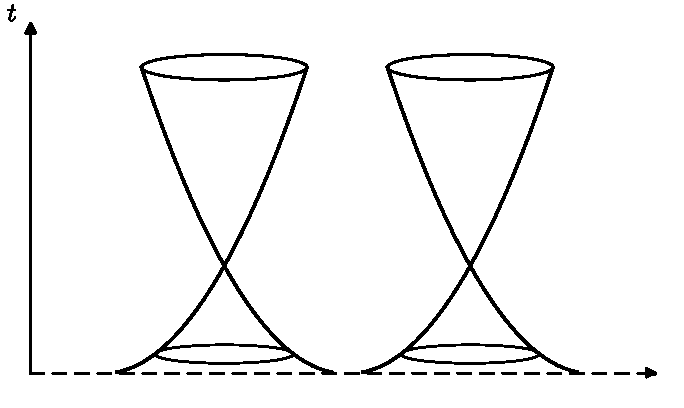
\includegraphics[width=0.72\textwidth]{fig_2.22.pdf}
\caption*{图 2.22\quad 平直 Robertson–Walker 宇宙（$a(t)\propto t^q$，$0<q<1$）的时空图。图中底部的虚线表示$t=0$处的奇点。由于光锥与奇点相切，两点的过去可以不重叠。}
\end{figure}
其中$x_0$是积分常数。这些曲线定义了我们这个膨胀宇宙的光锥，如图 2.22 所绘。由于我们已假定$0<q<1$，光锥在$t=0$处与奇点相切。这个几何的一个关键特征是：两点的光锥在过去未必相交；这与 Minkowski 空间形成对照——在 Minkowski 空间中，任何两点的光锥在过去和未来都必定相交。我们说每个事件都定义了一个“视界”（horizon），在其之外存在对该事件处发生的事情不可能有任何影响的世界线。这是因为，既然没有任何东西能运动得比光快，每个点只能被那些或者位于其过去光锥之上、或者位于其内部的事件所影响（实际上，我们把过去光锥连同其内部合起来简称为一个事件的“过去”）。彼此处在对方视界之外的两个事件，称为“处于因果接触之外”（out of causal contact）。这些概念将在下一节以及第 4 章和第 8 章中得到更仔细的探讨。

\section{因果性}

许多物理问题都可以表述为初值问题（initial-value problem）：已知系统在某一时刻的状态，那么在稍后某时刻它的状态是什么？这类问题有确定答案，这件事归功于因果性（causality）——即这样一种观念：未来的事件可以被理解为初始条件加上物理定律所产生的后果。初值问题在 GR 中和在 Newton 物理学或狭义相对论中一样常见；然而，时空背景的动力学本性为初值表述的失效引入了新的可能方式。这里我们非常简略地介绍一些概念，它们用于理解因果性在 GR 中如何起作用。
% ---- 书页 79 / p094 ----
我们将考察在固定的背景时空上演化物质场的问题，而不是度规本身的演化。我们的指导原则是：任何信号都不能传播得比光速快；因此信息只会沿类时或类光的轨迹流动（不一定是测地线）。由于有时需要区分纯类时的路径和仅仅是非类空的路径，我们定义\textbf{因果曲线}（causal curve）为处处类时或类光的曲线。于是，给定流形$M$的任意子集$S$，我们定义$S$的\textbf{因果未来}（causal future），记作$J^+(S)$，为沿指向未来的因果曲线从$S$出发所能到达的点集；\textbf{编时未来}（chronological future）$I^+(S)$则是沿指向未来的类时曲线所能到达的点集。注意，零长度的曲线是因果的，但不是编时的；因此，点$p$永远在自己的因果未来$J^+(p)$之中，却不一定在自己的编时未来$I^+(p)$之中（尽管也可能在，下面会提到）。因果过去$J^-$与编时过去$I^-$可以类似地定义。

$M$的子集$S$如果没有任何两点能用类时曲线相连，就称为\textbf{非编时的}（achronal）；例如，Minkowski 时空中任何无边缘的类空超曲面都是非编时的。给定一个闭的非编时集$S$，我们定义$S$的\textbf{未来依赖域}（future domain of dependence），记作$D^+(S)$，为所有这样的点$p$的集合：经过$p$的\emph{每一条}向过去行进的不可延伸因果曲线都必须与$S$相交。（不可延伸（inextendible）只是说这条曲线永远延伸下去，不在某个有限点处终止；闭则是说该集合的补集是开集。）$S$自身的元素也是$D^+(S)$的元素。把未来换成过去，同样定义过去依赖域$D^-(S)$。一般而言，$M$中有些点会落在某个依赖域之内，有些则在其外；我们把$D^+(S)$的边界定义为\textbf{未来 Cauchy 视界}（future Cauchy horizon）$H^+(S)$，类似地把$D^-(S)$的边界定义为过去 Cauchy 视界$H^-(S)$。你可以自行确信它们都是类光曲面。依赖域和 Cauchy 视界绘于图 2.23 中，图中$S$取为非编时曲面$\Sigma$的一个连通子集。

\begin{figure}[H]
\centering
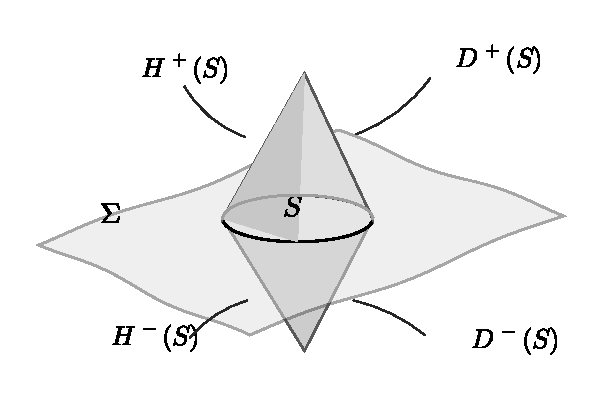
\includegraphics[width=0.72\textwidth]{fig_2.23.pdf}
\caption*{图 2.23\quad 类空曲面$\Sigma$的一个连通子集$S$及其因果结构。$D^\pm(S)$表示$S$的未来/过去依赖域，$H^\pm(S)$表示未来/过去 Cauchy 视界。}
\end{figure}
% ---- 书页 80 / p095 ----
这些定义的用处应当很明显：如果没有任何东西运动得比光快，信号就不可能传播到任一点$p$的光锥之外。因此，如果留在该光锥内部的每条曲线都必须与$S$相交，那么在$S$上给出的信息就应当足以预言$p$处的情形；也就是说，在$S$上给出的物质场的初始数据可以用来解出$p$处场的值。通过知道$S$上发生的事就能预言其情形的所有点的集合，是并集$D(S)=D^+(S)\cup D^-(S)$，简称\textbf{依赖域}（domain of dependence）。如果闭的非编时曲面$\Sigma$的依赖域$D(\Sigma)$是整个流形，就称$\Sigma$为\textbf{Cauchy 面}（Cauchy surface）；有了 Cauchy 面上给出的信息，我们就能预言整个时空中发生的事。如果一个时空拥有 Cauchy 面（它可能没有），就称它是\textbf{全局双曲}（globally hyperbolic）的。

\begin{figure}[H]
\centering
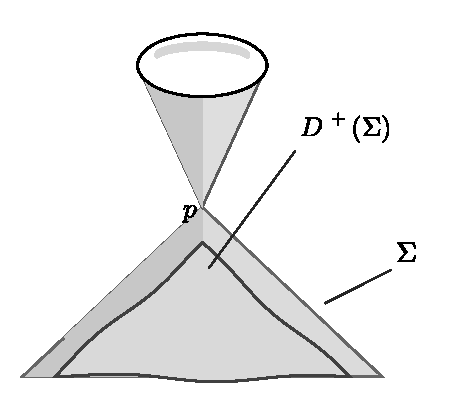
\includegraphics[width=0.72\textwidth]{fig_2.24.pdf}
\caption*{图 2.24\quad 曲面$\Sigma$处处类空，但处在点$p$的过去光锥的过去；它的依赖域并不是整个时空。}
\end{figure}
任何闭的、非编时的、且没有边缘的集合$\Sigma$都称为\textbf{部分 Cauchy 面}（partial Cauchy surface）。一个部分 Cauchy 面之所以未能成为真正的 Cauchy 面，可能归咎于它自己，也可能归咎于时空。一种可能性是我们恰好选了一张“坏”超曲面（尽管很难给出一个一般判据，说明超曲面何时在这种意义上是坏的）。考虑 Minkowski 空间以及一张无边缘的类空超曲面$\Sigma$，它停留在某个点的光锥的过去一侧，如图 2.24 所示。此时$\Sigma$是一张非编时曲面，但显然$D^+(\Sigma)$终止于光锥处，我们无法用$\Sigma$上的信息预言整个 Minkowski 空间中发生的事。当然，我们本可以挑别的曲面，使依赖域是整个流形，所以这件事并不怎么令我们担心。

Cauchy 视界出现的一种稍更不平凡的方式，是\textbf{闭合类时曲线}（closed timelike curves）的出现。在 Newton 物理学中，因果性靠时间的绝对观念冷酷无情地向前行进而得到强制。在狭义相对论中事情更加受限：你不仅必须在时间中前进，而且光速限制了你在空间中移动的迅捷程度（你必须待在自己的前向光锥之内）。在广义相对论中，你必须待在自己的前向光锥之内这一点仍然成立；然而它严格来说只是个局域的概念，因为从全局看，时空的曲率可能把光锥从一处“倾斜”到另一处。原则上，光锥可以被扭曲得足够厉害，使得一位观者能沿一条处处类时的前向路径运动，却与它自身在其“过去”的一点相交——这就是闭合类时曲线。

作为一个简单的例子，考虑一个带坐标$(t,x)$的二维几何，使坐标为$(t,x)$与$(t,x+1)$的点被等同起来。于是拓扑为$\mathbf{R}\times S^1$。我们取度规为
\begin{equation*}
ds^2=-\cos(\lambda)\,\mathrm{d}t^2-\sin(\lambda)\left[\mathrm{d}t\,\mathrm{d}x+\mathrm{d}x\,\mathrm{d}t\right]+\cos(\lambda)\,\mathrm{d}x^2,
\tag{2.63}
\end{equation*}
其中
\begin{equation*}
\lambda=\cot^{-1}t,
\tag{2.64}
\end{equation*}
% ---- 书页 81 / p096 ----
\begin{figure}[H]
\centering
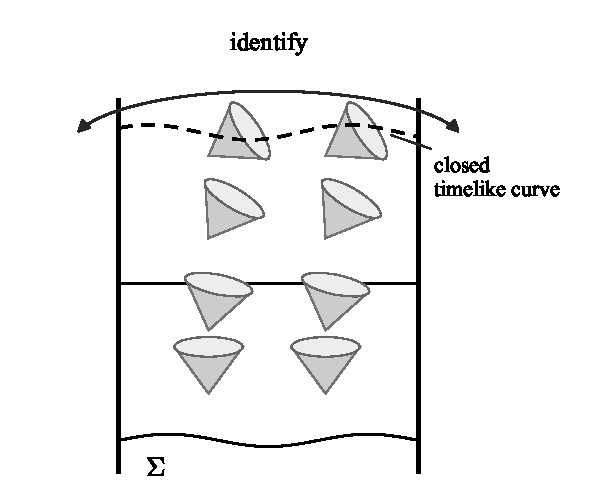
\includegraphics[width=0.72\textwidth]{fig_2.25.pdf}
\caption*{图 2.25\quad 一个带闭合类时曲线的柱状时空。光锥逐渐倾斜，使得曲面$\Sigma$的依赖域充满时空的下部，但当闭合类时曲线出现时，这个依赖域便告终结。}
\end{figure}
它从$\lambda(t=-\infty)=0$过渡到$\lambda(t=\infty)=\pi$。这个度规并不代表广义相对论的什么著名的特解，它只是被杜撰出来充当闭合类时曲线的一个有趣例子；不过有一个众所周知的例子叫 Misner 空间（Misner space），性质与此类似。在 (2.63) 定义的时空中，光锥随着你走向未来而逐渐倾斜，如图 2.25 所示。当$t<0$时，光锥指向前方，因果性得以维持。然而一旦$t>0$，$x$就变成了类时坐标，于是可以沿一条绕$S^1$一圈回到自身的类时轨迹运动；这就是一条闭合类时曲线。如果我们先前指定的曲面$\Sigma$位于该点的过去，那么含闭合类时曲线的区域中的任何点都不在$\Sigma$的依赖域之内，因为闭合类时曲线自身不与$\Sigma$相交。因此在曲面$t=0$处必然存在一个 Cauchy 视界。这显然是比前一例更糟的问题，因为在这个时空中似乎不存在良定义的初值问题。

\begin{figure}[H]
\centering
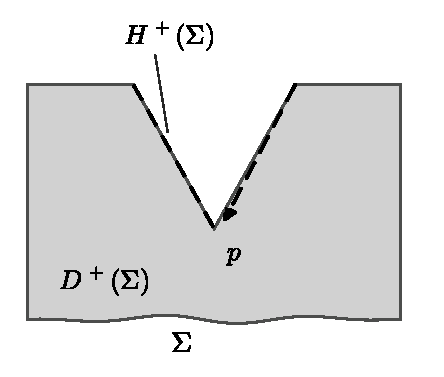
\includegraphics[width=0.72\textwidth]{fig_2.26.pdf}
\caption*{图 2.26\quad $p$处的一个奇点把位于其未来的一切点，都从位于其过去的曲面$\Sigma$的依赖域中除去。}
\end{figure}
最后一个例子由奇点的存在性提供：奇点是不在流形之中的点，尽管沿测地线走上有限距离就能到达它们。典型情形是曲率在某一点变为无穷大时出现奇点；一旦发生，这一点就不能再算是时空的一部分。这种情形可以导致 Cauchy 视界的出现，如图 2.26 所绘——点$p$处于某个奇点的未来，它就不可能位于该奇点过去某张超曲面的依赖域之内，因为从$p$出发会有一些曲线径直终止在奇点上。
% ---- 书页 82 / p097 ----
当我们试图从初始数据演化度规自身时，这些障碍同样会出现在 GR 的初值问题中。然而，它们的麻烦程度各不相同。挑到一张“坏”初始超曲面的可能性并不常出现，尤其因为大多数解都是（通过在整个时空中求解 Einstein 方程）全局地找到的。你必须小心的唯一情形是 Einstein 方程的数值求解：超曲面选得不好会导致数值困难，即使原则上完全解存在。闭合类时曲线似乎是 GR 极力避免的东西——肯定有包含它们的解，但从一般的初始数据演化通常不会产生它们。而奇点实际上不可避免。引力总是吸引的这一简单事实倾向于把物质拉到一起，使曲率增大，一般会导致某种奇点。显然我们必须学会与此共处，尽管存在这样的希望：一个良定义的量子引力理论会消除（或至少教会我们如何对付）经典 GR 的奇点。

\section{张量密度}

张量具有令人信服的美与简洁，但有些时候考虑非张量的对象是有用的。回忆第 1 章中我们引入的完全反对称的 Levi–Civita 符号，定义为
\begin{equation*}
\tilde\epsilon_{\mu_1\mu_2\cdots\mu_n}=
\begin{cases}
+1 & \text{若 $\mu_1\mu_2\cdots\mu_n$ 是 $01\cdots(n-1)$ 的偶置换（even permutation），}\\
-1 & \text{若 $\mu_1\mu_2\cdots\mu_n$ 是 $01\cdots(n-1)$ 的奇置换，}\\
0 & \text{其他情形。}
\end{cases}
\tag{2.65}
\end{equation*}
根据定义，Levi–Civita 符号在\emph{任何坐标系}中都具有上面规定的分量（至少在任何右手坐标系中是如此；交换手性会把$\tilde\epsilon_{\mu_1\mu_2\cdots\mu_n}$的分量乘上一个整体负号）。它之所以被称为“符号”，当然是因为它不是张量；它被定义为在坐标变换下不变。我们之所以只能在平直时空的惯性坐标中把它当作张量来处理，是因为洛伦兹变换反正不会改变其分量。它的行为可以与普通张量的行为联系起来，方法是首先注意到：给定任何$n\times n$矩阵$M^\mu{}_{\mu'}$，行列式$|M|$满足
\begin{equation*}
\tilde\epsilon_{\mu'_1\mu'_2\cdots\mu'_n}|M|=\tilde\epsilon_{\mu_1\mu_2\cdots\mu_n}\,M^{\mu_1}{}_{\mu'_1}M^{\mu_2}{}_{\mu'_2}\cdots M^{\mu_n}{}_{\mu'_n}.
\tag{2.66}
\end{equation*}
这不过是任何矩阵的行列式的一个紧凑表达式，与用代数余子式（cofactor）矩阵写出的通常公式完全等价。（你可以对$2\times2$或$3\times3$矩阵自行验证。）于是，令$M^\mu{}_{\mu'}=\partial x^\mu/\partial x^{\mu'}$，我们就得到
% ---- 书页 83 / p098 ----
\begin{equation*}
\tilde\epsilon_{\mu'_1\mu'_2\cdots\mu'_n}=\left|\frac{\partial x^{\mu'}}{\partial x^\mu}\right|\tilde\epsilon_{\mu_1\mu_2\cdots\mu_n}\,\frac{\partial x^{\mu_1}}{\partial x^{\mu'_1}}\frac{\partial x^{\mu_2}}{\partial x^{\mu'_2}}\cdots\frac{\partial x^{\mu_n}}{\partial x^{\mu'_n}},
\tag{2.67}
\end{equation*}
其中我们还利用了这样两个事实：矩阵$\partial x^{\mu'}/\partial x^\mu$是$\partial x^\mu/\partial x^{\mu'}$的逆，而逆矩阵的行列式是行列式的逆，$|M^{-1}|=|M|^{-1}$。于是，Levi–Civita 符号的变换方式与张量变换规律很接近，只是前面多出一个行列式。按这种方式变换的对象称为\textbf{张量密度}（tensor densities）。另一个例子由度规的行列式$g=|g_{\mu\nu}|$给出。容易验证，对 (2.48) 两边取行列式，就得到坐标变换下
\begin{equation*}
g(x^{\mu'})=\left|\frac{\partial x^{\mu'}}{\partial x^\mu}\right|^{-2}g(x^\mu).
\tag{2.68}
\end{equation*}
因此$g$也不是张量；它的变换方式与 Levi–Civita 符号类似，只是把雅可比行列式取到了$-2$次幂。雅可比行列式所取的幂称为张量密度的\textbf{权}（weight）；Levi–Civita 符号是权为 1 的密度，而$g$是权为$-2$的（标量）密度。

不过，我们不像喜欢张量那样喜欢张量密度。有一个简单的办法可以把密度变成诚实的张量——乘以$|g|^{w/2}$，其中$w$是密度的权（加绝对值符号是因为对洛伦兹型度规有$g<0$）。结果将按张量变换规律变换。因此，例如，我们可以把\textbf{Levi–Civita 张量}（Levi–Civita tensor）定义为
\begin{equation*}
\boxed{\ \epsilon_{\mu_1\mu_2\cdots\mu_n}=\sqrt{|g|}\,\tilde\epsilon_{\mu_1\mu_2\cdots\mu_n}.\ }
\tag{2.69}
\end{equation*}
由于这是一个真正的张量，我们可以升降指标等等。有时人们会定义一个带上指标的 Levi–Civita 符号版本$\tilde\epsilon^{\mu_1\mu_2\cdots\mu_n}$，其分量在数值上等于$\mathrm{sgn}(g)\tilde\epsilon_{\mu_1\mu_2\cdots\mu_n}$，其中$\mathrm{sgn}(g)$是度规行列式的符号。结果发现这是一个权为$-1$的密度，它与带上指标的张量（用$g^{\mu\nu}$把$\epsilon_{\mu_1\mu_2\cdots\mu_n}$的指标升起即得）之间的关系为
\begin{equation*}
\epsilon^{\mu_1\mu_2\cdots\mu_n}=\frac{1}{\sqrt{|g|}}\,\tilde\epsilon^{\mu_1\mu_2\cdots\mu_n}.
\tag{2.70}
\end{equation*}
你最终经常会做的事情之一，是把$\epsilon^{\mu_1\mu_2\cdots\mu_n}$的$p$个指标与$\epsilon_{\mu_1\mu_2\cdots\mu_n}$缩并；结果可以用 Kronecker δ 的反对称化乘积表示为
\begin{equation*}
\epsilon^{\mu_1\mu_2\cdots\mu_p\alpha_1\cdots\alpha_{n-p}}\epsilon_{\mu_1\mu_2\cdots\mu_p\beta_1\cdots\beta_{n-p}}=(-1)^s p!(n-p)!\,\delta^{[\alpha_1}_{\beta_1}\cdots\delta^{\alpha_{n-p}]}_{\beta_{n-p}},
\tag{2.71}
\end{equation*}
其中$s$是度规负本征值的个数（按我们的约定，洛伦兹号差下$s=1$）。最常见的例子是$p=n-1$，
% ---- 书页 84 / p099 ----
对此我们有
\begin{equation*}
\epsilon^{\mu_1\mu_2\cdots\mu_{n-1}\alpha}\epsilon_{\mu_1\mu_2\cdots\mu_{n-1}\beta}=(-1)^s (n-1)!\,\delta^\alpha_\beta.
\tag{2.72}
\end{equation*}

\section{微分形式}

现在让我们引入一类特殊的张量，称为\textbf{微分形式}（differential forms，或简称形式（form））。一个微分$p$形式不过是一个完全反对称的$(0,p)$型张量。于是，标量自动就是 0-形式，对偶矢量自动就是 1-形式（这就解释了此前的术语）。我们还有 4-形式$\epsilon_{\mu\nu\rho\sigma}$。所有$p$形式的空间记作$\Lambda^p$，流形$M$上所有$p$形式场的空间记作$\Lambda^p(M)$。一个半直截了当的组合练习揭示出，$n$维矢量空间上线性独立的$p$形式共有$n!/(p!(n-p)!)$个。于是在四维时空的一点上，有一个线性独立的 0-形式、四个 1-形式、六个 2-形式、四个 3-形式和一个 4-形式。$p>n$时不存在$p$形式，因为由反对称性，所有分量都自动为零。

为什么我们要在乎微分形式？这个问题不加些功夫难以回答，但基本想法是：形式既可以被微分，也可以被积分，而不需要任何额外几何结构的帮助。我们将对这两种操作各作一番简要的浏览。

给定一个$p$形式$A$和一个$q$形式$B$，取反对称化的张量积，我们可以构造出一个$(p+q)$形式，称为\textbf{楔积}（wedge product）$A\wedge B$：
\begin{equation*}
(A\wedge B)_{\mu_1\cdots\mu_{p+q}}=\frac{(p+q)!}{p!\,q!}\,A_{[\mu_1\cdots\mu_p}B_{\mu_{p+1}\cdots\mu_{p+q}]}.
\tag{2.73}
\end{equation*}
于是，例如两个 1-形式的楔积就是
\begin{equation*}
(A\wedge B)_{\mu\nu}=2A_{[\mu}B_{\nu]}=A_\mu B_\nu-A_\nu B_\mu.
\tag{2.74}
\end{equation*}
注意
\begin{equation*}
A\wedge B=(-1)^{pq}B\wedge A,
\tag{2.75}
\end{equation*}
所以只要你小心对待符号，就可以改变楔积的顺序。使用形式时我们可以随意省略指标，因为我们知道所有指标都在下边，而且张量是完全反对称的。

\textbf{外微分}（exterior derivative）$\mathrm{d}$使我们能够对$p$形式场求微分而得到$(p+1)$形式场。它定义为适当归一化的、反对称化的偏导数：
\begin{equation*}
(\mathrm{d}A)_{\mu_1\cdots\mu_{p+1}}=(p+1)\partial_{[\mu_1}A_{\mu_2\cdots\mu_{p+1}]}.
\tag{2.76}
\end{equation*}
最简单的例子是梯度，它就是 0-形式的外微分：
\begin{equation*}
(\mathrm{d}\phi)_\mu=\partial_\mu\phi.
\tag{2.77}
\end{equation*}

% ---- 书页 85 / p100 ----
外微分算符作用在 $p$-形式 $\omega$ 与 $q$-形式 $\eta$ 的乘积上时，服从一种修正版的莱布尼茨（Leibniz）法则：
\begin{equation*}
\mathrm{d}(\omega\wedge\eta)=(\mathrm{d}\omega)\wedge\eta+(-1)^{p}\,\omega\wedge(\mathrm{d}\eta). \tag{2.78}
\end{equation*}
我们鼓励你们自己证明这一点。

外微分值得特别关注的原因在于，它\emph{是一个张量}，即使在弯曲时空中也是如此；这一点与它的近亲——偏导数——不同。对于 $p=1$，我们可以从 1-形式的偏导数的变换律，即式 (2.38)，看出这一点；其中那个碍事的非张量项可以写成
\begin{equation*}
W_{\nu}\frac{\partial x^{\mu}}{\partial x^{\mu'}}\frac{\partial}{\partial x^{\mu}}\frac{\partial x^{\nu}}{\partial x^{\nu'}}=W_{\nu}\frac{\partial^{2}x^{\nu}}{\partial x^{\mu'}\partial x^{\nu'}}. \tag{2.79}
\end{equation*}
由于偏导数相互对易，这个表达式在 $\mu'$ 与 $\nu'$ 下是对称的。而外微分被定义为反对称化的偏导数，所以这一项会消失（对称表达式的反对称部分为零）。于是剩下的就是正确的张量变换律；推广到任意 $p$ 也很直接。所以外微分是一个堂堂正正的张量算符；然而，它并不能完全替代偏导数，因为它只对形式有定义。下一章我们将定义协变导数，它更接近我们通常所设想的“偏导数向任意流形的推广”。

关于外微分运算，另一个有趣的事实是：对任何形式 $A$，
\begin{equation*}
\mathrm{d}(\mathrm{d}A)=0, \tag{2.80}
\end{equation*}
它也常写作 $\mathrm{d}^{2}=0$。这一恒等式是 $\mathrm{d}$ 的定义以及偏导数可对易这一事实的推论：作用在任何对象上都有 $\partial_{\alpha}\partial_{\beta}=\partial_{\beta}\partial_{\alpha}$。这把我们引向下面一段数学题外话，纯粹为了好玩。我们把一个 $p$-形式 $A$ 定义为\textbf{闭}（closed）的，如果 $\mathrm{d}A=0$；称它是\textbf{恰当}（exact）的，如果 $A=\mathrm{d}B$，其中 $B$ 是某个 $(p-1)$-形式。显然，所有恰当形式都是闭形式，但反之则未必成立。在流形 $M$ 上，闭 $p$-形式构成一个矢量空间 $Z^{p}(M)$，恰当形式构成一个矢量空间 $B^{p}(M)$。我们定义一个新的矢量空间，其元素称为上同调类（cohomology class），即闭形式模掉恰当形式所得的空间：
\begin{equation*}
H^{p}(M)=\frac{Z^{p}(M)}{B^{p}(M)}. \tag{2.81}
\end{equation*}
也就是说，两个闭形式［$Z^{p}(M)$ 的元素］如果相差一个恰当形式［$B^{p}(M)$ 的元素］，它们就定义同一个上同调类［$H^{p}(M)$ 的元素］。奇妙的是，上同调空间 $H^{p}(M)$ 的维数只依赖于流形 $M$ 的拓扑。Minkowski 空间在拓扑上等价于 $\mathbf{R}^{4}$，后者乏味得很，于是当 $p>0$ 时所有的 $H^{p}(M)$ 都为零；而 $p=0$ 时我们有 $H^{0}(M)=\mathbf{R}$。因此在 Minkowski 空间中，除了零形式之外，所有闭形式都是恰当的；零形式不可能是恰当形式，因为根本不存在 $-1$-形式，可以让零形式成为其外微分。
% ---- 书页 86 / p101 ----
以这种方式抽取出关于拓扑的信息，着实令人惊讶，而这本质上涉及的是微分方程的解。

我们将要介绍的最后一种作用于微分形式的运算是\textbf{Hodge 对偶性}（Hodge duality）。我们在 $n$ 维流形上定义\textbf{Hodge 星算符}（Hodge star operator），它是一个从 $p$-形式到 $(n-p)$-形式的映射，
\begin{equation*}
(*A)_{\mu_{1}\cdots\mu_{n-p}}=\frac{1}{p!}\epsilon^{\nu_{1}\cdots\nu_{p}}{}_{\mu_{1}\cdots\mu_{n-p}}A_{\nu_{1}\cdots\nu_{p}}, \tag{2.82}
\end{equation*}
它把 $A$ 映为“$A$ 的对偶”。与我们其他作用于形式的运算不同，Hodge 对偶确实依赖于流形的度规［这一点应当显而易见，因为为了定义式 (2.82)，我们不得不提升了 Levi-Civita 张量的某些指标］。将 Hodge 星算符作用两次，得到的要么是原形式本身，要么是相差一个正负号的原形式：
\begin{equation*}
**A=(-1)^{s+p(n-p)}A, \tag{2.83}
\end{equation*}
其中 $s$ 是度规本征值中负号的个数。

关于 Hodge 对偶有两个事实。第一，Hodge 意义上的“对偶性”有别于矢量与对偶矢量之间的关系。“对偶性”的观念是指从一个空间到另一个空间的变换，其性质是把该变换做两次就回到原来的空间。矢量与 1-形式之间的对偶，以及 $p$-形式与 $(n-p)$-形式之间的 Hodge 对偶，对二者而言这一点都成立，这应当是清楚的。矢量空间之间对偶性的一个要求是：原来的空间与变换后的空间具有相同的维数；$p$-形式空间与 $(n-p)$-形式空间正是如此。

第二个事实涉及三维欧几里得空间中的微分形式。两个 1-形式的楔积的 Hodge 对偶给出另一个 1-形式：
\begin{equation*}
*(U\wedge V)_{i}=\epsilon_{i}{}^{jk}U_{j}V_{k}. \tag{2.84}
\end{equation*}
（所有前面的系数都恰好相消。）由于欧几里得空间中的 1-形式就像矢量一样，我们得到了一个从两个矢量到单个矢量的映射。你们应当让自己确信，这正是通常的叉乘（cross product）；而且 Levi-Civita 张量的出现解释了为什么叉乘在宇称变换下变号（两个坐标互换，等价地，基矢互换）。这正是叉乘只存在于三维的原因——因为只有在三维，我们才有一个从两个对偶矢量到第三个对偶矢量的有趣映射。

电动力学为微分形式的应用提供了一个格外有说服力的例子。从外微分的定义可以清楚地看到，方程 (1.97) 可以被简洁地表述为 2-形式 $F_{\mu\nu}$ 的闭性：
\begin{equation*}
\mathrm{d}F=0. \tag{2.85}
\end{equation*}
这是否意味着 $F$ 也是恰当的？是的；正如我们已指出的，Minkowski 空间拓扑平凡，所以所有闭形式都是恰当的。因此必定存在某个 1-形式 $A_{\mu}$，使得
\begin{equation*}
F=\mathrm{d}A. \tag{2.86}
\end{equation*}
% ---- 书页 87 / p102 ----
这个 1-形式就是大家熟悉的电磁学中的\textbf{矢势}（vector potential），其 0 分量由标势给出，$A_{0}=\Phi$，正如我们在第 1 章中讨论过的那样。规范不变性（gauge invariance）表现为：理论在 $A\to A+\mathrm{d}\lambda$ 下不变，其中 $\lambda$ 是某个标量（零形式）；从关系式 (2.86) 出发，这一点也是显而易见的。麦克斯韦方程组中的另一条，即 (1.96)，则可以表述为 3-形式之间的一个方程：
\begin{equation*}
\mathrm{d}(*F)=*J, \tag{2.87}
\end{equation*}
其中电流 1-形式 $J$ 不过是降低了指标的电流四维矢量。把细节补全就留给你们了，这是把微分形式记号转换为普通指标记号的绝佳练习。

Hodge 对偶性与某些场论的一个迷人性质密切相关：强耦合与弱耦合之间的对偶。很难不注意到，方程 (2.85) 与 (2.87) 看起来非常相似。的确，如果令 $J_{\mu}=0$，方程在如下“对偶变换”下不变：
\begin{gather*}
F\to *F,\\
*F\to -F. \tag{2.88}
\end{gather*}
因此我们说，真空中的麦克斯韦方程组是对偶不变的，而电荷的存在会破坏这种不变性。我们可以设想，自然界中除了电单极子之外还存在磁单极子；那样我们就可以在 (2.85) 的右端加上一个磁流项 $*J_{M}$，方程就会在下述组合下不变：对偶变换再加上一个额外的替换 $J\leftrightarrow J_{M}$。（当然，(2.85) 的右端若非零就与 $F=\mathrm{d}A$ 不相容，所以这个想法只有在 $A_{\mu}$ 不是基本变量时才行得通。）Dirac 考虑过磁单极子的想法，并证明了它们存在的一个必要条件：基本磁单极荷必须与基本电荷成反比。如今，基本电荷是一个小数目；电动力学是\emph{弱耦合}（weakly coupled）的，这正是微扰论在量子电动力学（QED）中如此惊人成功的原因。但 Dirac 关于磁荷的条件意味着，一个对偶变换会把一个弱耦合电荷的理论变成一个强耦合磁单极子的理论（反之亦然）。遗憾的是，磁单极子不太容易纳入普通电磁学，所以这些想法并不能直接应用；不过某种对偶对称性可能存在于某些理论之中（比如超对称非阿贝尔规范理论）。如果它确实存在，我们就有机会通过考察弱耦合的对偶版本，来分析一个看似强耦合（因而难以求解）的理论；在某些理论中，实际发生的正是这种情形。我们希望这些技术将使我们能够探索强耦合量子场论中确然存在的各种现象，比如夸克在强子中的禁闭。
% ---- 书页 88 / p103 ----

\section{积分}

张量密度与微分形式的一个重要应用场合是流形上的积分。你们大概已经接触过这样的事实：在 $\mathbf{R}^{n}$ 上的普通微积分中，体积元 $d^{n}x$ 在坐标变换下会多出一个雅可比行列式因子：
\begin{equation*}
d^{n}x'=\left|\frac{\partial x^{\mu'}}{\partial x^{\mu}}\right|d^{n}x. \tag{2.89}
\end{equation*}
其实，从微分形式的观点出发，这个公式有一个漂亮的解释，它来自如下事实：\emph{在 $n$ 维流形 $M$ 上，被积函数应当被恰当地理解为 $n$-形式。}换句话说，$n$ 维区域 $\Sigma\subset M$ 上的积分是一个从 $n$-形式场 $\omega$ 到实数的映射：
\begin{equation*}
\int_{\Sigma}:\omega\to\mathbf{R}. \tag{2.90}
\end{equation*}
这样的说法初听起来可能有些奇怪，但在曲线积分的语境里它肯定显得眼熟。在一维情形，任何一个 1-形式都可以写成 $\omega=\omega(x)\mathrm{d}x$，其中第一个 $\omega$ 是 1-形式，$\omega(x)$ 表示（唯一的那一个）分量函数。确实，我们把一维积分写成 $\int\omega(x)\mathrm{d}x$；你们也许习惯于把符号 $\mathrm{d}x$ 想成一个无穷小距离，但更确切地说，它是一个微分形式。

为了把这一点弄得更清楚，考虑不止一维的情形。如果我们宣称被积对象是一个 $n$-形式，就需要解释它在什么意义上是反对称的，而且顺便还要解释它为什么根本就是一个 $(0,n)$ 张量（从 $n$ 个矢量构成的集合到 $\mathbf{R}$ 的线性映射）。我们都同意积分可以写成 $\int f(x)\,d\mu$，其中 $f(x)$ 是流形上的标量函数，$d\mu$ 是体积元，或者叫测度。体积元的作用是给每个（无穷小的）区域指定一个（无穷小的）实数，即该区域的体积。无穷小区域（相对于有限大小的区域）的一个好处是，它们可以取成矩形的平行六面体——在存在曲率时，我们对“矩形平行六面体”应当是什么意思并没有清楚的概念，但当我们在无穷小区域中工作时，曲率的效应可以忽略。显然我们在这里并不严谨，但我们当下的目的纯粹是建立动机。

\begin{figure}[H]
\centering
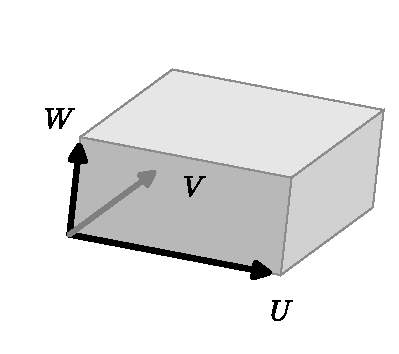
\includegraphics[width=0.72\textwidth]{fig_2.27.pdf}
\caption*{图 2.27\quad 一个无穷小的 $n$ 维区域，表示为一个平行六面体，由 $n$ 个矢量构成的有序集合定义，图中记为 $U$、$V$、$W$。}
\end{figure}
如图 2.27 所示（为了便于说明，我们把流形取成三维的），一个平行六面体由定义其棱边的 $n$ 个矢量确定。于是，我们的体积元应当是一个从 $n$ 个矢量到实数的映射：$d\mu(U,V,W)\in\mathbf{R}$。（严格说来，它应当是一个从无穷小矢量到无穷小数的映射，但这样的映射同样会把有限矢量映到有限的数。）同样清楚的是，它应当可以按实数线性缩放；如果我们改变任何一个定义矢量的长度，体积就会相应地改变：$d\mu(aU,bV,cW)=abc\,d\mu(U,V,W)$。至于对矢量相加的线性性，就不是那么显而易见了，不过你们可以通过画图让自己信服。
% ---- 书页 89 / p104 ----
因此，我们的体积元是一个名副其实的 $(0,n)$ 张量。为什么反对称？因为我们定义的是一个有向的（oriented）对象；如果交换其中两个矢量，得到的体积应当大小相同而符号相反。（如果这一点不明显，你们至少应当让自己相信：当两个矢量共线时，体积应当为零。）这样，$n$ 维情形下的体积元在非常切实的意义上就是 $n$-形式。

要做实际计算，我们需要把这些想法变得更具体，而这其实很简单。关键的洞察是：把朴素的体积元 $d^{n}x$ 等同于用楔积构造出来的一个反对称张量密度：
\begin{equation*}
d^{n}x=\mathrm{d}x^{0}\wedge\cdots\wedge\mathrm{d}x^{n-1}. \tag{2.91}
\end{equation*}
右边的表达式可能有误导性，因为它看上去像一个张量（准确说是一个 $n$-形式），但其实是一个密度。当然，如果我们在 $M$ 上有两个函数 $f$ 和 $g$，那么 $\mathrm{d}f$ 和 $\mathrm{d}g$ 是 1-形式，而 $\mathrm{d}f\wedge\mathrm{d}g$ 是 2-形式。但出现在 (2.91) 中的函数是坐标函数本身，所以当我们变换坐标时，是把 1-形式 $\mathrm{d}x^{\mu}$ 换成一组新的 $\mathrm{d}x^{\mu'}$。你们看这里滑稽的地方——通常坐标变换改变的是分量，而不是 1-形式本身。(2.91) 的右端是一个依赖于坐标的对象（精确地说，是一个张量密度），它在 $x^{\mu}$ 坐标系中的行为就如同 $\mathrm{d}x^{0}\wedge\cdots\wedge\mathrm{d}x^{n-1}$。让我们看看它的实际运作。首先注意到，楔积的定义允许我们写出
\begin{equation*}
\mathrm{d}x^{0}\wedge\cdots\wedge\mathrm{d}x^{n-1}=\frac{1}{n!}\tilde{\epsilon}_{\mu_{1}\cdots\mu_{n}}\mathrm{d}x^{\mu_{1}}\wedge\cdots\wedge\mathrm{d}x^{\mu_{n}}, \tag{2.92}
\end{equation*}
这是因为楔积与 Levi-Civita 符号都是完全反对称的。（$1/n!$ 这个因子负责处理对指标的排列求和所引入的重复计数。）在坐标变换下，$\tilde{\epsilon}_{\mu_{1}\cdots\mu_{n}}$ 保持不变，而各个 1-形式按照式 (2.26) 变换，这就导致
\begin{align*}
\tilde{\epsilon}_{\mu_{1}\cdots\mu_{n}}\mathrm{d}x^{\mu_{1}}\wedge\cdots\wedge\mathrm{d}x^{\mu_{n}}&=\tilde{\epsilon}_{\mu_{1}\cdots\mu_{n}}\frac{\partial x^{\mu_{1}}}{\partial x^{\mu_{1}'}}\cdots\frac{\partial x^{\mu_{n}}}{\partial x^{\mu_{n}'}}\mathrm{d}x^{\mu_{1}'}\wedge\cdots\wedge\mathrm{d}x^{\mu_{n}'}\\
&=\left|\frac{\partial x^{\mu}}{\partial x^{\mu'}}\right|\tilde{\epsilon}_{\mu_{1}'\cdots\mu_{n}'}\mathrm{d}x^{\mu_{1}'}\wedge\cdots\wedge\mathrm{d}x^{\mu_{n}'}. \tag{2.93}
\end{align*}
在两边同乘雅可比行列式，并利用 (2.91) 与 (2.92)，便回到了 (2.89)。

显然，朴素的体积元 $d^{n}x$ 是按密度而非按张量变换的；不过，只要乘上 $\sqrt{|g|}$，就能直接构造出一个不变的体积元：
\begin{equation*}
\sqrt{|g'|}\,\mathrm{d}x^{0'}\wedge\cdots\wedge\mathrm{d}x^{(n-1)'}=\sqrt{|g|}\,\mathrm{d}x^{0}\wedge\cdots\wedge\mathrm{d}x^{n-1}, \tag{2.94}
\end{equation*}
它当然就正是 $(n!)^{-1}\epsilon_{\mu_{1}\cdots\mu_{n}}\mathrm{d}x^{\mu_{1}}\wedge\cdots\wedge\mathrm{d}x^{\mu_{n}}$。为简单起见，我们通常把体积元写成 $\sqrt{|g|}\,d^{n}x$，而不写成显式的楔积：
% ---- 书页 90 / p105 ----
\begin{equation*}
\sqrt{|g|}\,d^{n}x\equiv\sqrt{|g|}\,\mathrm{d}x^{0}\wedge\cdots\wedge\mathrm{d}x^{n-1}\ ; \tag{2.95}
\end{equation*}
心里记住它本应是一个 $n$-形式，就足够了。事实上，体积元不多不少，恰恰就是 Levi-Civita 张量 $\epsilon_{\mu_{1}\cdots\mu_{n}}$；把基 1-形式显式地补写回来，我们看到
\begin{align*}
\epsilon&\equiv\epsilon_{\mu_{1}\cdots\mu_{n}}\mathrm{d}x^{\mu_{1}}\otimes\cdots\otimes\mathrm{d}x^{\mu_{n}}\\
&=\frac{1}{n!}\epsilon_{\mu_{1}\cdots\mu_{n}}\mathrm{d}x^{\mu_{1}}\wedge\cdots\wedge\mathrm{d}x^{\mu_{n}}\\
&=\frac{1}{n!}\sqrt{|g|}\,\tilde{\epsilon}_{\mu_{1}\cdots\mu_{n}}\mathrm{d}x^{\mu_{1}}\wedge\cdots\wedge\mathrm{d}x^{\mu_{n}}\\
&=\sqrt{|g|}\,\mathrm{d}x^{0}\wedge\cdots\wedge\mathrm{d}x^{n-1}\\
&\equiv\sqrt{|g|}\,d^{n}x. \tag{2.96}
\end{align*}
注意到，epsilon 张量引入的组合因子，恰好与从张量积换成楔积时引入的因子相消；之所以允许做这种替换，是因为 epsilon 张量会自动反对称化。

于是，结论很简单：标量函数 $\phi$ 在 $n$ 维流形上的积分 $I$ 写作
\begin{equation*}
\boxed{I=\int\phi(x)\sqrt{|g|}\,d^{n}x.} \tag{2.97}
\end{equation*}
给定 $\phi(x)$ 和 $\sqrt{|g|}$ 的显式表达式，这样的积分就可以用多变量微积分的通常方法直接算出。度规的行列式所起的作用是自动保证正确的变换性质。你们有时会看到更抽象的记号
\begin{equation*}
I=\int\phi(x)\,\epsilon\ ; \tag{2.98}
\end{equation*}
鉴于 (2.96)，这两种写法传递的是同样的内容。

\section{习题}

% 习题编号照原书
\textbf{1.}\quad 一个流形在拓扑上非平凡，并不必然意味着它不能用单个卡片覆盖。与圆周 $S^{1}$ 的情形相对照，请通过显式地构造映射，证明无穷长圆柱 $\mathbf{R}\times S^{1}$ 可以只用一个卡片覆盖。

\textbf{2.}\quad 通过巧妙地选取坐标卡片，我们能让 $\mathbf{R}^{2}$ 看起来像一个一维流形吗？能让 $\mathbf{R}^{1}$ 看起来像一个二维流形吗？如果能，请显式构造一个适当的图册；如果不能，请解释为什么不能。这个问题的要点在于促使你深入思考流形究竟是什么；若不进一步讨论拓扑空间的更多细节，就无法严格地回答它。特别是，你可能必须忘掉你在原来的 $\mathbf{R}^{2}$ 或 $\mathbf{R}^{1}$ 中已经知道的那套“开集”定义，而把它们定义为恰当地继承自所映射到的 $\mathbf{R}^{1}$ 或 $\mathbf{R}^{2}$。

% ---- 书页 91 / p106 ----
\textbf{3.}\quad 请通过显式构造一个适当的图册，证明二维环面 $T^{2}$ 是一个流形。（显然，不必是极大的图册。）

\textbf{4.}\quad 验证 2.3 节末尾关于两个矢量场的对易子所作的那些论断（线性性、Leibniz 律、分量公式、作为一个矢量场的变换）。

\textbf{5.}\quad 在 $\mathbf{R}^{2}$ 中给出两个线性无关、处处不为零的矢量场的例子，使它们的对易子不为零。注意，这两个场在每一点都给出切空间的一组基，但由于对易子不为零，它不可能是坐标基。

\textbf{6.}\quad 把 $\mathbf{R}^{3}$ 看作一个带有平直欧几里得度规的流形，坐标为 $\{x,y,z\}$。引入球坐标 $\{r,\theta,\phi\}$，其与 $\{x,y,z\}$ 的关系为
\begin{gather*}
x=r\sin\theta\cos\phi\\
y=r\sin\theta\sin\phi\\
z=r\cos\theta, \tag{2.99}
\end{gather*}
于是度规取如下形式
\begin{equation*}
ds^{2}=\mathrm{d}r^{2}+r^{2}\mathrm{d}\theta^{2}+r^{2}\sin^{2}\theta\,\mathrm{d}\phi^{2}. \tag{2.100}
\end{equation*}

\textbf{(a)}\quad 一个粒子沿如下参数化曲线运动：
\begin{equation*}
x(\lambda)=\cos\lambda,\qquad y(\lambda)=\sin\lambda,\qquad z(\lambda)=\lambda. \tag{2.101}
\end{equation*}
请在 $\{r,\theta,\phi\}$ 系中表出这条曲线的路径。

\textbf{(b)}\quad 分别在笛卡尔坐标系与球坐标系中，计算该曲线的切矢量的分量。

\textbf{7.}\quad 长椭球坐标（prolate spheroidal coordinates）可以用来简化天体力学中的 Kepler 问题。它们与欧几里得三维空间中通常的笛卡尔坐标 $(x,y,z)$ 的关系为
\begin{gather*}
x=\sinh\chi\,\sin\theta\cos\phi,\\
y=\sinh\chi\,\sin\theta\sin\phi,\\
z=\cosh\chi\,\cos\theta.
\end{gather*}
把注意力限制在 $y=0$ 的平面上，回答下列问题。

\textbf{(a)}\quad 联系 $(x,z)$ 与 $(\chi,\theta)$ 的坐标变换矩阵 $\partial x^{\mu}/\partial x^{\nu'}$ 是什么？

\textbf{(b)}\quad 线元 $ds^{2}$ 在长椭球坐标下是什么样子？

\textbf{8.}\quad 验证式 (2.78)：对 $p$-形式 $\omega$ 与 $q$-形式 $\eta$ 的乘积的外微分，我们有
\begin{equation*}
\mathrm{d}(\omega\wedge\eta)=(\mathrm{d}\omega)\wedge\eta+(-1)^{p}\,\omega\wedge(\mathrm{d}\eta). \tag{2.102}
\end{equation*}

% ---- 书页 92 / p107 ----
\textbf{9.}\quad 在 Minkowski 空间中，设 $*F=q\sin\theta\,\mathrm{d}\theta\wedge\mathrm{d}\phi$。

\textbf{(a)}\quad 计算 $\mathrm{d}*F=*J$。

\textbf{(b)}\quad 2-形式 $F$ 等于什么？

\textbf{(c)}\quad 对这个解来说，电场与磁场分别等于什么？

\textbf{(d)}\quad 计算 $\int_{V}\mathrm{d}*F$，其中 $V$ 是在某个固定时刻、欧几里得三维空间中半径为 $R$ 的一个球。

\textbf{10.}\quad 考虑二维时空中的麦克斯韦方程组 $\mathrm{d}F=0$、$\mathrm{d}*F=*J$。解释为什么这两组方程中可以舍弃一组。证明电磁场可以用一个标量场表出，并写出这个标量场的场方程的分量形式。

\textbf{11.}\quad 本题为一个非常简单的问题附加了大量动机性的文字；别因此分心。在与点粒子相联系的普通电磁学中，作用量中代表规范势 1-形式 $A^{(1)}$ 与带电粒子相耦合的部分可以写成 $S=\int_{\gamma}A^{(1)}$，其中 $\gamma$ 是粒子的世界线。（$A^{(1)}$ 的上标只是为了提醒你它是一个 1-形式。）本题中你要考虑一个与普通电磁学有亲缘关系的理论，但这一次是在 11 维时空里，带有 3-形式规范势 $A^{(3)}$ 和 4-形式场强 $F^{(4)}=\mathrm{d}A^{(3)}$。注意，场强在规范变换 $A^{(3)}\to A^{(3)}+\mathrm{d}\lambda^{(2)}$（$\lambda^{(2)}$ 为任意 2-形式）下不变。

\textbf{(a)}\quad 这种规范场自然与之耦合的对象，其空间维数应当是多少？（例如，普通电磁学（E+M）与零维对象——点粒子——相耦合。）

\textbf{(b)}\quad 普通电子的电荷由如下积分给出：2-形式规范场强的对偶在围绕粒子的一个二维球面上的积分。对于 $A^{(3)}$ 所耦合的对象，你会如何定义它的“电荷”？请论证：如果 $\mathrm{d}*F^{(4)}=0$，这个荷是守恒的。

\textbf{(c)}\quad 设想存在一个“对偶规范势” $\widetilde{A}$，满足 $\mathrm{d}(\widetilde{A})=*F^{(4)}$。它自然与之耦合的对象是多少维的？

\textbf{(d)}\quad 规范场自身的作用量（相对于它与其他对象的耦合而言）将是整个 11 维时空上的一个积分。这样的作用量中，容许出现而且在“局域”规范变换下不变的项有哪些？例如，规范变换可以由一个在无穷远处为零的 2-形式 $\lambda^{(2)}$ 来规定。请把自己限制在关于 $A^{(3)}$ 及其一阶导数的线性、二次或三次的项（不含二阶导数，不含更高阶的项）。你可以使用外微分、楔积和 Hodge 对偶，但不允许度规的任何显式出现。

更多的背景知识：“超对称性”（supersymmetry）是一种假想中的对称性，它把玻色子（自旋为整数的粒子）与费米子（自旋为 $\frac{1}{2}$、$\frac{3}{2}$ 等的粒子）联系起来。一个有趣的性质是，超对称理论只有在 11 维或更低维数中才是良定义的——在更高的维数下，超对称性将要求存在自旋大于 2 的粒子，而这样的粒子无法自洽地量子化。十一维超对称是一个独一无二的理论，它自然地包含一个 3-形式规范势（更不用说引力了）。近期的工作表明，它还包含本题所暗指的各种更高维的对象（尽管我们在这里走了些捷径）。这个理论最终被发现是某个称作 $M$-理论（M-theory）的东西的一个良定义的极限，而 $M$-理论的其他极限则是各种 10 维超弦理论。

 % 本文件由 scripts/assemble.py 自动装配，勿手改（改 parts/ 后重跑）
% 第3章 曲率

% 第3章 Curvature
\chapter{曲率}

\section{概述}

我们都知道曲率是什么意思，至少是非正式地知道；而且在本书前两章里，我们一直随意地不时提及曲率这个概念，却从未认真定义过它。显然，曲率以某种方式依赖于度规（metric），度规定义了我们流形的几何；但如何把曲率归属于任何一个给定的度规，并不是一目了然的（因为正如我们所见，即使是平直空间的度规，在一个足够“铺张”的坐标系里也可以显得任意复杂）。数学中常见的情况是：要把我们关于一个概念的直觉形式化为可用的数学结构，需要相当多的细心；把我们所想的“曲率”形式化，正是本章的主题。

我们即将发展出来的技巧对本学科至关重要；可以放心地说，这一章每页有用公式的密度比其他任何一章都高。让我们快速总结一下其中最重要的那些，为接下来的形式体系提供一张路线图。

曲率表现自身的所有方式都依赖于一种叫做“联络”（connection）的东西，它为我们提供了一种联系相邻点的切空间中矢量的途径。存在一个唯一的、可以由度规构造出来的联络，它浓缩在一个叫做 Christoffel 符号（Christoffel symbol）的对象之中：
\begin{equation*}
\Gamma^\lambda_{\mu\nu} = \frac{1}{2} g^{\lambda\sigma}\left(\partial_\mu g_{\nu\sigma} + \partial_\nu g_{\sigma\mu} - \partial_\sigma g_{\mu\nu}\right).
\tag{3.1}
\end{equation*}

这种记号让 $\Gamma^\lambda_{\mu\nu}$ 看起来像一个张量，但事实上它不是；这就是为什么我们把它叫做一个“对象”（object）或“符号”（symbol）。联络最基本的用途是用来取协变导数（covariant derivative）$\nabla_\mu$（偏导数的推广）；矢量场 $V^\nu$ 的协变导数为
\begin{equation*}
\nabla_\mu V^\nu = \partial_\mu V^\nu + \Gamma^\nu_{\mu\sigma} V^\sigma\,,
\tag{3.2}
\end{equation*}
而其他种类的张量的协变导数也由类似的表达式给出。联络还出现在测地线（geodesic，直线概念的推广）的定义中。参数化曲线 $x^\mu(\lambda)$ 是测地线，如果它满足
\begin{equation*}
\frac{d^2 x^\mu}{d\lambda^2} + \Gamma^\mu_{\rho\sigma}\frac{d x^\rho}{d\lambda}\frac{d x^\sigma}{d\lambda} = 0,
\tag{3.3}
\end{equation*}
这就是著名的测地线方程（geodesic equation）。

最后，曲率的技术性表述包含在 Riemann 曲率张量（Riemann tensor）之中，它是一个 $(1,3)$ 型张量，由联络构造出来：
\begin{equation*}
R^\rho{}_{\sigma\mu\nu} = \partial_\mu \Gamma^\rho_{\nu\sigma} - \partial_\nu \Gamma^\rho_{\mu\sigma} + \Gamma^\rho_{\mu\lambda}\Gamma^\lambda_{\nu\sigma} - \Gamma^\rho_{\nu\lambda}\Gamma^\lambda_{\mu\sigma}.
\tag{3.4}
\end{equation*}
我们想了解的关于流形曲率的一切都由 Riemann 张量给出；当且仅当度规完全平直时它才为零。广义相对论的 Einstein 方程把这个张量的某些分量与能量-动量张量联系起来。

这四个公式在弯曲流形的研究中都具有头等重要性。接下来我们将会看到，它们是如何从对平直空间中那些熟悉的几何观念如何适应于这个更一般背景的细致考察中产生出来的。

\section{协变导数}

在我们对流形的讨论中，有一点已经很清楚：流形一旦定义，就有各种各样可以谈论的概念了——我们可以定义函数、求导数、考虑参数化路径、搭建张量，等等。而另一些概念，比如一个区域的体积或一条路径的长度，则需要额外的某种结构，也就是度规的引入。把曲率这个概念想成是只依赖于度规的东西，似乎是很自然的。然而，在更仔细的处理中我们会发现，曲率依赖于联络，而联络依赖于或不依赖于度规皆有可能。尽管如此，我们也将证明，度规的存在蕴含着一个唯一确定的联络，这个联络的曲率可以看作是该度规的曲率。这正是广义相对论中使用的那个联络，所以在这个特定背景下，把曲率看作刻画度规的性质而不引入任何附加结构，是合理的。

当我们试图处理“偏导数不是一个好的张量算符”这一问题时，联络就成为必要的了。我们想要的是一个协变导数（covariant derivative），即这样一个算符：在平直空间的惯性坐标下它还原为偏导数，而在任意流形上它按张量方式变换。按惯例，人们会花不少篇幅来论证引入协变导数的动机，但实际上这个需求是显而易见的：诸如 $\partial_\mu T^{\mu\nu} = 0$ 这样的方程总得设法推广到弯曲空间去。所以我们就一致同意：协变导数是个好东西，值得拥有，然后着手把它建立起来。

在惯性坐标下的平直空间中，偏导数算符 $\partial_\mu$ 是一个从 $(k,l)$ 型张量场到 $(k,l+1)$ 型张量场的映射，它对其自变量的作用是线性的，并且在张量积上满足 Leibniz 律。在我们现在想要考虑的更一般的情形下，这一切仍然成立，但偏导数所提供的这个映射依赖于所用的坐标系。因此我们想定义一个协变导数（covariant derivative）算符 $\nabla$ 来行使偏导数的职能，但要以一种与坐标无关的方式进行。与其直接假定答案（那样做其实完全可以接受），不如仔细想想偏导数的协变推广\emph{应该}具有些什么性质——数学结构毕竟是人类的发明，而不是躺在人行道上等着被捡到的。我们一开始先要求：$\nabla$ 是一个从 $(k,l)$ 型张量场到 $(k,l+1)$ 型张量场的映射，并且具有下面两条性质：
\begin{enumerate}
\item 线性性：$\nabla(T + S) = \nabla T + \nabla S$；
\item Leibniz（乘积）律：$\nabla(T \otimes S) = (\nabla T)\otimes S + T\otimes(\nabla S)$.
\end{enumerate}

如果 $\nabla$ 要服从 Leibniz 律，那么它总可以写成偏导数再加上某个线性变换的形式。也就是说，取协变导数时我们先取偏导数，然后施加一个修正，使结果成为协变的。【这个听起来挺合理的论断我们不打算证明；感兴趣的读者可参阅 Wald (1984)。】让我们考虑这对矢量 $V^\nu$ 的协变导数意味着什么。它意味着：对每个方向 $\mu$，协变导数 $\nabla_\mu$ 将由偏导数 $\partial_\mu$ 加上一个修正给出，该修正由一组 $n$ 个矩阵 $(\Gamma_\mu)^\rho{}_\sigma$ 规定（对每个 $\mu$ 有一个 $n\times n$ 矩阵，其中 $n$ 是流形的维数）。实际上这对括号通常被省掉，这些矩阵——即所谓的\emph{联络系数}（connection coefficients）——以一种随意的指标位置写成为 $\Gamma^\rho_{\mu\sigma}$。于是我们有
\begin{equation*}
\boxed{\;\nabla_\mu V^\nu = \partial_\mu V^\nu + \Gamma^\nu_{\mu\lambda} V^\lambda.\;}
\tag{3.5}
\end{equation*}

注意在第二项里，原来在 $V$ 上的指标跑到了 $\Gamma$ 上，同时有一个新的指标被求和。如果这就是用偏导数表出的矢量协变导数，那么我们应该能通过要求左边是一个 $(1,1)$ 型张量，来确定 $\Gamma^\nu_{\mu\lambda}$ 的变换性质。也就是说，我们希望变换规律是
\begin{equation*}
\nabla_{\mu'} V^{\nu'} = \frac{\partial x^\mu}{\partial x^{\mu'}}\frac{\partial x^{\nu'}}{\partial x^\nu}\nabla_\mu V^\nu.
\tag{3.6}
\end{equation*}
让我们先看左边；可以用式 (3.5) 把它展开，再变换那些我们已经理解的部分（也就是除了 $\Gamma^{\nu'}_{\mu'\lambda'}$ 之外的全部）：
\begin{align*}
\nabla_{\mu'} V^{\nu'} &= \partial_{\mu'} V^{\nu'} + \Gamma^{\nu'}_{\mu'\lambda'} V^{\lambda'}\\
&= \frac{\partial x^\mu}{\partial x^{\mu'}}\frac{\partial x^{\nu'}}{\partial x^\nu}\partial_\mu V^\nu + \frac{\partial x^\mu}{\partial x^{\mu'}}V^\nu\frac{\partial}{\partial x^\mu}\frac{\partial x^{\nu'}}{\partial x^\nu} + \Gamma^{\nu'}_{\mu'\lambda'}\frac{\partial x^{\lambda'}}{\partial x^\lambda}V^\lambda.
\tag{3.7}
\end{align*}
在右边，我们同样可以把 $\nabla_\mu V^\nu$ 展开：
\begin{equation*}
\frac{\partial x^\mu}{\partial x^{\mu'}}\frac{\partial x^{\nu'}}{\partial x^\nu}\nabla_\mu V^\nu = \frac{\partial x^\mu}{\partial x^{\mu'}}\frac{\partial x^{\nu'}}{\partial x^\nu}\partial_\mu V^\nu + \frac{\partial x^\mu}{\partial x^{\mu'}}\frac{\partial x^{\nu'}}{\partial x^\nu}\Gamma^\nu_{\mu\lambda}V^\lambda.
\tag{3.8}
\end{equation*}
最后这两个表达式应当相等；两边的第一项完全相同因而抵消，于是我们得到
\begin{equation*}
\Gamma^{\nu'}_{\mu'\lambda'}\frac{\partial x^\lambda}{\partial x^{\lambda'}}V^\lambda + \frac{\partial x^\mu}{\partial x^{\mu'}}V^\lambda\frac{\partial}{\partial x^\mu}\frac{\partial x^{\nu'}}{\partial x^\lambda} = \frac{\partial x^\mu}{\partial x^{\mu'}}\frac{\partial x^{\nu'}}{\partial x^\nu}\Gamma^\nu_{\mu\lambda}V^\lambda,
\tag{3.9}
\end{equation*}
这里我们把一个哑指标从 $\nu$ 改成了 $\lambda$。这个方程对任意矢量 $V^\lambda$ 都必须成立，所以我们可以在两边把它消去。然后，通过乘上 $\partial x^\lambda/\partial x^{\sigma'}$ 并把 $\sigma'$ 重新标记为 $\lambda'$，就可以把带撇坐标中的联络系数孤立出来。结果是
\begin{equation*}
\Gamma^{\nu'}_{\mu'\lambda'} = \frac{\partial x^\mu}{\partial x^{\mu'}}\frac{\partial x^\lambda}{\partial x^{\lambda'}}\frac{\partial x^{\nu'}}{\partial x^\nu}\Gamma^\nu_{\mu\lambda} + \frac{\partial x^\mu}{\partial x^{\mu'}}\frac{\partial x^\lambda}{\partial x^{\lambda'}}\frac{\partial^2 x^{\nu'}}{\partial x^\mu\partial x^\lambda}.
\tag{3.10}
\end{equation*}
当然，这并不是张量的变换规律——右边的第二项把它破坏了。不过没关系，因为\emph{联络系数并不是某个张量的分量}。它们是被有意构造成非张量的，但构造的方式使得式 (3.5) 这个组合按张量变换——偏导数变换中多出来的项与 $\Gamma$ 变换中多出来的项恰好抵消。正因如此，我们对联络系数的指标位置并不那么讲究；它们不是张量，所以你应当尽量不要对它们作指标的升降。

那么其他种类的张量的协变导数呢？通过与矢量情形类似的推理，1-形式（one-form）的协变导数同样可以表示为偏导数加上某个线性变换。但迄今为止还没有任何理由认为，表示这个变换的矩阵应当与系数 $\Gamma^\nu_{\mu\lambda}$ 有什么关系。一般地，我们可以写出类似
\begin{equation*}
\nabla_\mu\omega_\nu = \partial_\mu\omega_\nu + \widetilde{\Gamma}^\lambda_{\mu\nu}\,\omega_\lambda,
\tag{3.11}
\end{equation*}
其中 $\widetilde{\Gamma}^\lambda_{\mu\nu}$ 是对每个 $\mu$ 的一组新矩阵。请注意各种不同的指标各自都在什么位置。可以直接推导出，$\widetilde{\Gamma}$ 的变换性质必须与 $\Gamma$ 相类似，否则 $\nabla_\mu\omega_\nu$ 就不会按张量变换；但除此之外，两者之间没有任何已确立的关系。为了确立这种关系，除了上面那两条性质之外，我们还需要再引入两条我们希望协变导数具有的性质：
\begin{enumerate}
\setcounter{enumi}{2}
\item 与缩并可交换：$\nabla_\mu(T^\lambda{}_{\lambda\rho}) = (\nabla T)_\mu{}^\lambda{}_{\lambda\rho}$，
\item 在标量上还原为偏导数：$\nabla_\mu\phi = \partial_\mu\phi$.
\end{enumerate}

没有办法“推导”出这些性质；我们只是要求它们作为协变导数定义的一部分而成立。注意，性质 3 等价于说 Kronecker delta（恒等映射）是协变常数的（covariantly constant）：$\nabla_\mu\delta^\lambda_\sigma = 0$；这当然是一个合理的要求。

让我们看看这些新性质蕴含着什么。给定某个 1-形式场 $\omega_\mu$ 和矢量场 $V^\mu$，我们可以对由 $\omega_\lambda V^\lambda$ 定义的标量取协变导数，得到
\begin{align*}
\nabla_\mu(\omega_\lambda V^\lambda) &= (\nabla_\mu\omega_\lambda)V^\lambda + \omega_\lambda(\nabla_\mu V^\lambda)\\
&= (\partial_\mu\omega_\lambda)V^\lambda + \widetilde{\Gamma}^\sigma_{\mu\lambda}\omega_\sigma V^\lambda + \omega_\lambda(\partial_\mu V^\lambda) + \omega_\lambda\Gamma^\lambda_{\mu\rho}V^\rho.
\tag{3.12}
\end{align*}
但由于 $\omega_\lambda V^\lambda$ 是一个标量，它也必须可以由偏导数给出：
\begin{align*}
\nabla_\mu(\omega_\lambda V^\lambda) &= \partial_\mu(\omega_\lambda V^\lambda)\\
&= (\partial_\mu\omega_\lambda)V^\lambda + \omega_\lambda(\partial_\mu V^\lambda).
\tag{3.13}
\end{align*}
只有当式 (3.12) 中带联络系数的那些项彼此抵消时，这才可能成立；也就是说，重新安排哑指标后，我们必须有
\begin{equation*}
0 = \widetilde{\Gamma}^\sigma_{\mu\lambda}\omega_\sigma V^\lambda + \Gamma^\sigma_{\mu\lambda}\omega_\sigma V^\lambda.
\tag{3.14}
\end{equation*}
但 $\omega_\sigma$ 和 $V^\lambda$ 都是完全任意的，所以
\begin{equation*}
\widetilde{\Gamma}^\sigma_{\mu\lambda} = -\Gamma^\sigma_{\mu\lambda}.
\tag{3.15}
\end{equation*}
我们所施加的这两个附加条件，于是使我们能够用与矢量情形相同的联络系数来表达 1-形式的协变导数，只是现在带一个负号（并且指标的搭配方式略有不同）：
\begin{equation*}
\boxed{\;\nabla_\mu\omega_\nu = \partial_\mu\omega_\nu - \Gamma^\lambda_{\mu\nu}\,\omega_\lambda.\;}
\tag{3.16}
\end{equation*}

联络系数编码了对任意阶张量取协变导数所需的全部信息，这应当不足为怪。这个公式相当直截了当：对每个上指标，引入一个带单个 $+\Gamma$ 的项；对每个下指标，引入一个带单个 $-\Gamma$ 的项：
\begin{align*}
\nabla_\sigma T^{\mu_1\mu_2\cdots\mu_k}{}_{\nu_1\nu_2\cdots\nu_l} ={}& \partial_\sigma T^{\mu_1\mu_2\cdots\mu_k}{}_{\nu_1\nu_2\cdots\nu_l}\\
&+ \Gamma^{\mu_1}_{\sigma\lambda}T^{\lambda\mu_2\cdots\mu_k}{}_{\nu_1\nu_2\cdots\nu_l} + \Gamma^{\mu_2}_{\sigma\lambda}T^{\mu_1\lambda\cdots\mu_k}{}_{\nu_1\nu_2\cdots\nu_l} + \cdots\\
&- \Gamma^{\lambda}_{\sigma\nu_1}T^{\mu_1\mu_2\cdots\mu_k}{}_{\lambda\nu_2\cdots\nu_l} - \Gamma^{\lambda}_{\sigma\nu_2}T^{\mu_1\mu_2\cdots\mu_k}{}_{\nu_1\lambda\cdots\nu_l} - \cdots.
\tag{3.17}
\end{align*}

这就是协变导数的一般表达式。你可以自行验证它；它来自我们所建立的这组公理，再加上“各类张量都是与坐标无关的实体”这一通常要求。有时人们使用另一种记号：正如用逗号表示偏导数，用分号表示协变导数：
\begin{equation*}
\nabla_\sigma T^{\mu_1\mu_2\cdots\mu_k}{}_{\nu_1\nu_2\cdots\nu_l} \equiv T^{\mu_1\mu_2\cdots\mu_k}{}_{\nu_1\nu_2\cdots\nu_l;\sigma}.
\tag{3.18}
\end{equation*}
再一次强调，在本书中我们将坚持使用“$\nabla_\sigma$”。
那么，要定义一个协变导数，我们需要在流形上放一个联络，它在某个坐标系中由一组系数 $\Gamma^\lambda_{\mu\nu}$ 规定（在 $n=4$ 维时有 $n^3=64$ 个独立分量），这些系数按式 (3.10) 变换。（“联络”（connection）这个名字来源于这样一个事实：它被用来把矢量从一个切空间输运到另一个切空间，我们很快就会看到；它有时用来指算符 $\nabla$，有时用来指系数 $\Gamma^\lambda_{\mu\nu}$。）显然，我们可以在任何流形上定义出许许多多联络，而每一个都蕴含着一种互不相同的协变微分的概念。在广义相对论中，这种自由度不是什么大问题，因为事实表明每个度规都定义一个唯一的联络，这正是 GR 中使用的那一个。让我们看看这是如何做到的。

首先要注意到，两个联络之差是一个张量。设想我们定义了两种不同的协变导数 $\nabla_\mu$ 和 $\widehat{\nabla}_\mu$，分别带有相联系的联络系数 $\Gamma^\lambda_{\mu\nu}$ 和 $\widehat{\Gamma}^\lambda_{\mu\nu}$。那么差
\begin{equation*}
S^\lambda{}_{\mu\nu} = \Gamma^\lambda_{\mu\nu} - \widehat{\Gamma}^\lambda_{\mu\nu}
\tag{3.19}
\end{equation*}
是一个 $(1,2)$ 型张量。（注意我们不得不为指标的摆放选定一个约定。）我们可以用蛮力来证明这一点，即代入联络系数的变换规律，但让我们稍微俏皮一点。给定一个任意矢量场 $V^\lambda$，我们知道 $\nabla_\mu V^\lambda$ 和 $\widehat{\nabla}_\mu V^\lambda$ 都是张量，因此它们的差也必是张量。这个差就是
\begin{align*}
\nabla_\mu V^\lambda - \widehat{\nabla}_\mu V^\lambda &= \partial_\mu V^\lambda + \Gamma^\lambda_{\mu\nu}V^\nu - \partial_\mu V^\lambda - \widehat{\Gamma}^\lambda_{\mu\nu}V^\nu\\
&= S^\lambda{}_{\mu\nu}V^\nu.
\tag{3.20}
\end{align*}
由于 $V^\lambda$ 是任意的，而左边是张量，所以 $S^\lambda{}_{\mu\nu}$ 必定是张量。作为一个平凡的推论，我们得知任何一组联络系数都可以表示为某个基准联络（fiducial connection）加上一个张量性的修正：
\begin{equation*}
\Gamma^\lambda_{\mu\nu} = \widehat{\Gamma}^\lambda_{\mu\nu} + S^\lambda{}_{\mu\nu}.
\tag{3.21}
\end{equation*}

接下来注意，给定一个由 $\Gamma^\lambda_{\mu\nu}$ 规定的联络，我们可以仅仅通过交换下指标立即构造出另一个联络。也就是说，系数集合 $\Gamma^\lambda_{\nu\mu}$ 也将按式 (3.10) 变换（因为出现在最后一项中的偏导数可以交换次序），所以它们确定一个互不相同的联络。这样一来，就有了一个可以与任何给定联络相联系的张量，即所谓的\emph{挠率张量}（torsion tensor），其定义为
\begin{equation*}
T^\lambda{}_{\mu\nu} = \Gamma^\lambda_{\mu\nu} - \Gamma^\lambda_{\nu\mu} = 2\Gamma^\lambda_{[\mu\nu]}.
\tag{3.22}
\end{equation*}
显然，挠率在其下指标上是反对称的，而在下指标上对称的联络被称为“无挠的”（torsion-free）。

现在我们可以在一个带有度规 $g_{\mu\nu}$ 的流形上，通过引入两条附加性质来定义一个唯一的联络：
\begin{itemize}
\item 无挠：$\Gamma^\lambda_{\mu\nu} = \Gamma^\lambda_{(\mu\nu)}$；
\item 度规相容性（metric compatibility）：$\nabla_\rho g_{\mu\nu} = 0$.
\end{itemize}

如果一个联络对度规取的协变导数处处为零，就称这个联络是\emph{度规相容}的（metric compatible）。这蕴含着几个不错的性质。第一，容易证明，Levi–Civita 张量和逆度规的协变导数同样为零：
\begin{align*}
\nabla_\lambda\epsilon_{\mu\nu\rho\sigma} &= 0\\
\nabla_\rho g^{\mu\nu} &= 0.
\tag{3.23}
\end{align*}
第二，度规相容的协变导数与指标的升降可以交换次序。于是，对某个矢量场 $V^\lambda$，
\begin{equation*}
g_{\mu\lambda}\nabla_\rho V^\lambda = \nabla_\rho(g_{\mu\lambda}V^\lambda) = \nabla_\rho V_\mu.
\tag{3.24}
\end{equation*}
如果联络不是度规相容的，那么在取协变导数时我们就得对指标的摆放非常小心。

因此，我们的论断是：在一个给定的流形上，与该流形上某个给定度规相容的无挠联络恰好只有一个。我们并不想把这两条要求纳入协变导数的定义；它们只不过是从许多可能的联络中挑出了一个。

我们可以通过推导出联络系数用度规表示的一个明显唯一的表达式，来同时证明存在性与唯一性。为此，我们把度规相容性方程按指标的三种不同排列展开：
\begin{align*}
\nabla_\rho g_{\mu\nu} &= \partial_\rho g_{\mu\nu} - \Gamma^\lambda_{\rho\mu}g_{\lambda\nu} - \Gamma^\lambda_{\rho\nu}g_{\mu\lambda} = 0\\
\nabla_\mu g_{\nu\rho} &= \partial_\mu g_{\nu\rho} - \Gamma^\lambda_{\mu\nu}g_{\lambda\rho} - \Gamma^\lambda_{\mu\rho}g_{\nu\lambda} = 0\\
\nabla_\nu g_{\rho\mu} &= \partial_\nu g_{\rho\mu} - \Gamma^\lambda_{\nu\rho}g_{\lambda\mu} - \Gamma^\lambda_{\nu\mu}g_{\rho\lambda} = 0.
\tag{3.25}
\end{align*}
从第一式中减去第二式和第三式，并利用联络的对称性，得到
\begin{equation*}
\partial_\rho g_{\mu\nu} - \partial_\mu g_{\nu\rho} - \partial_\nu g_{\rho\mu} + 2\Gamma^\lambda_{\mu\nu}g_{\lambda\rho} = 0.
\tag{3.26}
\end{equation*}
乘上 $g^{\rho\sigma}$ 之后即可直接解出联络。结果是
\begin{equation*}
\boxed{\;\Gamma^\sigma_{\mu\nu} = \frac{1}{2}g^{\sigma\rho}\left(\partial_\mu g_{\nu\rho} + \partial_\nu g_{\rho\mu} - \partial_\rho g_{\mu\nu}\right).\;}
\tag{3.27}
\end{equation*}
这个公式是本学科中最重要的公式之一；请把它牢牢记在心里。当然，我们只是证明了：如果度规相容且无挠的联络存在，它就必须具有式 (3.27) 的形式；你可以自行验证，式 (3.27) 的右边的确像联络一样变换。
我们从度规推导出的这个联络，正是传统的广义相对论所依据的联络。它有着不同的名字：有时叫 \emph{Christoffel 联络}，有时叫 \emph{Levi–Civita 联络}，有时叫 \emph{Riemann 联络}。与之相联系的联络系数有时被称为 \emph{Christoffel 符号}（Christoffel symbols），并写成 $\left\{^{\sigma}_{\mu\nu}\right\}$ 的样子；我们有时也会把它们叫做 Christoffel 符号，但不会使用这种古怪的记号。研究带有度规及其相应联络的流形的学问叫做黎曼几何（Riemannian geometry）；当度规具有洛伦兹号差时，有时也称为伪黎曼几何（pseudo-Riemannian geometry）。

在让我们的协变导数开工之前，应该先提几点杂七杂八的性质。首先，注意在通常的平直空间里，其实存在一个我们无时无刻不在使用的隐式联络——由平直度规构造出来的 Christoffel 联络。平直空间中 Christoffel 联络的系数在笛卡尔坐标下为零，但在曲线坐标系下则不然。以极坐标下的平面为例，其度规为
\begin{equation*}
ds^2 = dr^2 + r^2d\theta^2.
\tag{3.28}
\end{equation*}
逆度规的非零分量很容易求出，为 $g^{rr} = 1$ 和 $g^{\theta\theta} = r^{-2}$。注意，我们用 $r$ 和 $\theta$ 作指标，记号的含义一目了然。我们可以计算一个典型的联络系数：
\begin{align*}
\Gamma^r_{rr} &= \frac{1}{2}g^{r\rho}(\partial_r g_{r\rho} + \partial_r g_{\rho r} - \partial_\rho g_{rr})\\
&= \frac{1}{2}g^{rr}(\partial_r g_{rr} + \partial_r g_{rr} - \partial_r g_{rr})\\
&\quad + \frac{1}{2}g^{r\theta}(\partial_r g_{r\theta} + \partial_r g_{\theta r} - \partial_\theta g_{rr})\\
&= \frac{1}{2}(1)(0 + 0 - 0) + \frac{1}{2}(0)(0 + 0 - 0)\\
&= 0.
\tag{3.29}
\end{align*}
遗憾的是，它等于零。但并非所有系数都如此：
\begin{align*}
\Gamma^r_{\theta\theta} &= \frac{1}{2}g^{r\rho}(\partial_\theta g_{\theta\rho} + \partial_\theta g_{\rho\theta} - \partial_\rho g_{\theta\theta})\\
&= \frac{1}{2}g^{rr}(\partial_\theta g_{\theta r} + \partial_\theta g_{r\theta} - \partial_r g_{\theta\theta})\\
&= \frac{1}{2}(1)(0 + 0 - 2r)\\
&= -r.
\tag{3.30}
\end{align*}
继续埋头摇计算的手柄，最终我们发现
\begin{align*}
\Gamma^r_{\theta r} &= \Gamma^r_{r\theta} = 0\\
\Gamma^\theta_{rr} &= 0\\
\Gamma^\theta_{r\theta} &= \Gamma^\theta_{\theta r} = \frac{1}{r}\\
\Gamma^\theta_{\theta\theta} &= 0.
\tag{3.31}
\end{align*}
从这些以及类似的表达式出发，我们可以推导出曲线坐标系下发散、梯度和旋度的公式。

反过来说，即使在弯曲空间中，让 Christoffel 符号在某个单独的点上为零也仍然是可能的。这是因为，正如我们在上一章论证过的，总可以让度规的一阶导数在某点为零；于是由式 (3.27)，从这个度规导出的联络系数也将为零。当然，这只能在一点处成立，而不能在该点的某个邻域内都成立。我们将在 3.4 节更充分地讨论这一点。

另一个有用的性质是，矢量的散度（关于 Christoffel 联络）的公式有一个简化形式。$V^\mu$ 的协变散度为
\begin{equation*}
\nabla_\mu V^\mu = \partial_\mu V^\mu + \Gamma^\mu_{\mu\lambda}V^\lambda.
\tag{3.32}
\end{equation*}
容易证明 Christoffel 联络满足
\begin{equation*}
\Gamma^\mu_{\mu\lambda} = \frac{1}{\sqrt{|g|}}\partial_\lambda\sqrt{|g|},
\tag{3.33}
\end{equation*}
于是我们得到
\begin{equation*}
\nabla_\mu V^\mu = \frac{1}{\sqrt{|g|}}\partial_\mu\left(\sqrt{|g|}\,V^\mu\right).
\tag{3.34}
\end{equation*}
对更高阶张量的散度也有相应公式，但一般就没有这么大的简化了。

在 Stokes 定理的弯曲空间版本（见附录 E）中，我们使用的正是 Christoffel 协变导数。若 $V^\mu$ 是区域 $\Sigma$（其边界为 $\partial\Sigma$）上的矢量场，则 Stokes 定理为
\begin{equation*}
\boxed{\;\int_\Sigma \nabla_\mu V^\mu\sqrt{|g|}\,d^nx = \int_{\partial\Sigma} n_\mu V^\mu\sqrt{|\gamma|}\,d^{\,n-1}x,\;}
\tag{3.35}
\end{equation*}
其中 $n_\mu$ 垂直于 $\partial\Sigma$，而 $\gamma_{ij}$ 是 $\partial\Sigma$ 上的诱导度规。如果联络不是度规相容的或不是无挠的，这个方程里就会多出一些附加的项。

最后需要提到的一点是：为了构造定义良好的张量，把偏导数换成协变导数并不总是必要的；特别是，外微分和矢量场的对易子都可以仅用偏导数良好地定义，这本质上是因为两者都涉及一个反对称化操作，它恰好抵消了偏导数变换规律中的非张量部分。同一特征也意味着，反过来，它们同样可以很好地用（无挠的）协变导数来定义；反对称化使联络系数的项归于消失。于是，若 $\nabla$ 是 Christoffel 联络，$\omega_\mu$ 是一个 1-形式，而 $X^\mu$ 和 $Y^\mu$ 是矢量场，则我们
可以写成
\begin{equation*}
(d\omega)_{\mu\nu} = 2\partial_{[\mu}\omega_{\nu]} = 2\nabla_{[\mu}\omega_{\nu]}
\tag{3.36}
\end{equation*}
以及
\begin{equation*}
[X,Y]^\mu = X^\lambda\partial_\lambda Y^\mu - Y^\lambda\partial_\lambda X^\mu = X^\lambda\nabla_\lambda Y^\mu - Y^\lambda\nabla_\lambda X^\mu.
\tag{3.37}
\end{equation*}
如果联络不是无挠的，这些表达式中的最后一个等号就不再成立；外微分和对易子更基本的定义是那些用偏导数表述的定义。

在继续往下讲之前，让我们回顾一下我们一步步给数学构造添加结构的过程。我们从“集合”这个基本概念出发，假定你对此已经熟悉（至少非正式地熟悉，如果不严格的话）。我们引入了集合的开子集的概念；这等价于引入一个拓扑，从而把集合提升为拓扑空间。然后，通过要求每个开集看起来都像 $\mathbf{R}^n$ 的一个区域（对每个集合 $n$ 相同），并且要求坐标卡片彼此光滑地缝合在一起，拓扑空间就变成了流形。流形同时是一种非常灵活又非常强有力的结构，它自然而然地配备了切丛、各种阶的张量丛、取外微分的能力，等等。接着我们继续在流形上放置度规，得到带度规的流形（有时称为黎曼流形）。我们发现，独立于度规也可以引入联络，从而使我们能够取协变导数。然而，一旦有了度规，就自动存在一个唯一的无挠且度规相容的联络。同样，我们也可以引入一个独立的体积形式，尽管它其实由度规自动确定。原则上，没有什么能阻止我们在任何一个给定流形上引入不止一个联络、或不止一个体积形式、或不止一个度规。在广义相对论中，我们确实拥有一个物理的度规，它同时决定体积和协变导数，所以这些概念的相互独立并不是一个关键特征。

\section{平行移动与测地线}

既然我们已经知道如何取协变导数，就让我们退后一步，把它放进更一般的微分框架中来考察。我们把导数看作量化“某个东西变化得有多快”的手段。对张量而言，关键问题是“相对于什么变化？”一个普通函数在时空每一点定义一个数，而比较两个不同的数是直截了当的，所以我们不必惊讶函数的偏导数在任意流形上依然有效。但张量是从矢量和 对偶矢量到实数的映射，要比较时空不同点上的这种映射，就不清楚该怎么做了。既然我们已经成功地构造了协变导数，能否把它看作某种意义上在量度张量的变化率？答案证明是肯定的：协变导数量度的正是张量场的瞬时变化率——与该张量倘若被“平行移动”将会成为的样子相比较。

\begin{figure}[H]
\centering
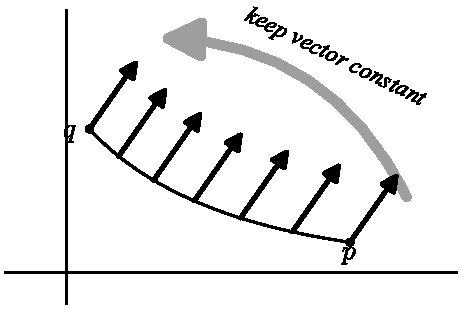
\includegraphics[width=0.72\textwidth]{fig_3.1.pdf}
\caption*{图 3.1\quad 在平直空间中，只需让矢量的笛卡尔（Cartesian）分量保持不变，我们就可以对矢量作平行移动。}
\end{figure}

换句话说，联络定义了一种让张量（沿某条路径）保持不变的具体方式，我们正是以此为基准来比较相邻的张量。

结果证明，平行移动这个概念本身就很有意思，值得花些时间思考。回忆一下，在平直空间中，我们不必太在意“矢量是定义在各个单独的点上的切空间的元素”这个事实；在平直空间中比较不同点上的矢量实际上是非常自然的（这里“比较”指的是相加、相减、取点积等等）。之所以自然，是因为在平直空间中，把一个矢量从一点移动到另一点同时保持它不变是有意义的，如图 3.1 所示。这样一来，一旦我们把矢量从一点搬到了另一点，就可以进行矢量空间中通常允许的那些运算。

把一个矢量沿一条路径移动而始终保持不变，这个概念就叫做\emph{平行移动}（parallel transport）。平行移动需要一个联络才能良好定义；在平直空间中对矢量的直观操作，暗含地使用了这个空间上的 Christoffel 联络。平直空间与弯曲空间的关键差别在于：在弯曲空间中，\emph{把一个矢量从一点平行移动到另一点，其结果将依赖于这两点之间所走的路径。}不必先把平行移动的完整机制拼装出来，我们就可以借助关于二维球面的直觉看清这一点。从赤道上的一个矢量开始，让它指向一条恒定经线的方向。用显而易见的方式沿一条经线把它平行移动到北极。然后取原来的矢量，先沿赤道把它平行移动一个角度 $\theta$，再像刚才那样把它移到北极。如图 3.2 所示，显然这个矢量沿两条路径平行移动后，到达了同一个目的地却带着两个不同的值（相差一个转动角 $\theta$）。

这样看来，似乎没有什么自然的方法能把一个矢量唯一地从一个切空间移动到另一个切空间；我们总可以对它作平行移动，但结果依赖于路径，而且走哪条路径也没有自然的选择。
\begin{figure}[H]
\centering
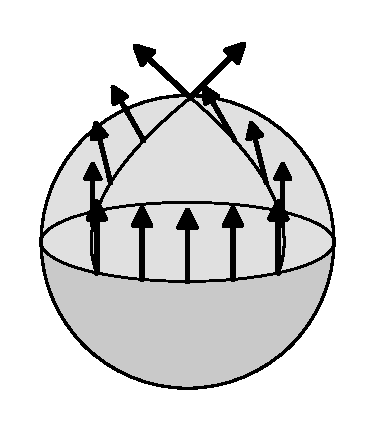
\includegraphics[width=0.72\textwidth]{fig_3.2.pdf}
\caption*{图 3.2\quad 二维球面上的平行移动。在弯曲流形上，平行移动的结果可能依赖于所走的路径。}
\end{figure}

与我们遇到过的某些问题不同，\emph{这个问题无解}——我们干脆必须学会与如下事实共处：只有当两个矢量属于同一切空间时，才能以自然的方式比较它们。例如，互相擦肩而过的两个粒子有良好定义的相对速度，它不能超过光速。但在弯曲流形上不同两点处的两个粒子却没有任何良好定义的相对速度概念——这个概念根本就没有意义。当然，在某些特殊情形下，把它说得好像有意义仍然是有用的，但偶然的用处不能代替严格的定义。例如在宇宙学中，来自遥远星系的光相对于我们从近处静止光源将会观测到的频率发生了红移。由于这个现象与相对运动引起的传统多普勒效应极为相似，我们非常想说，星系正以由其红移定义的速度“远离我们而去”。在严格的层面上这是无意义的胡话，是 Wittgenstein 所说的“语法错误”——星系并没有在退行，因为“它们相对于我们的速度”这个概念并非良好定义。实际发生的事情是：在我们与星系之间，时空度规沿着光子从这里到那里的路径发生了变化（宇宙膨胀了），导致光的波长增加。作为你怎样出错的一个例子：把多普勒公式天真地应用于星系红移，会推出某些星系的退行速度超光速，表面上与相对论矛盾。这个表观佯谬的解决很简单：星系“退行”这个概念本身就不应当按字面理解。

关于我们不能做的事说得够多了；让我们看看能做什么。平行移动被认为是“保持矢量不变”这个概念在弯曲空间中的推广：即当我们把矢量沿一条路径移动时保持它不变；对任意阶的张量亦然。
给定一条曲线 $x^\mu(\lambda)$，在平直空间中，张量 $T^{\mu_1\mu_2\cdots\mu_k}{}_{\nu_1\nu_2\cdots\nu_l}$ 沿这条曲线保持不变的要求，就是它的分量为常数：
\begin{equation*}
\frac{d}{d\lambda}T^{\mu_1\mu_2\cdots\mu_k}{}_{\nu_1\nu_2\cdots\nu_l} = \frac{dx^\mu}{d\lambda}\frac{\partial}{\partial x^\mu}T^{\mu_1\mu_2\cdots\mu_k}{}_{\nu_1\nu_2\cdots\nu_l} = 0.
\end{equation*}
为了使这一表述具有恰当的张量性，我们只需把这个偏导数换成协变导数，并定义\emph{方向协变导数}（directional covariant derivative）为
\begin{equation*}
\frac{D}{d\lambda} = \frac{dx^\mu}{d\lambda}\nabla_\mu.
\tag{3.38}
\end{equation*}
这是一个只在路径上有定义的映射，从 $(k,l)$ 型张量到 $(k,l)$ 型张量。于是我们把张量 $T$ 沿路径 $x^\mu(\lambda)$ 的\emph{平行移动}（parallel transport）定义为：$T$ 沿路径的协变导数为零这一要求：
\begin{equation*}
\left(\frac{D}{d\lambda}T\right)^{\mu_1\mu_2\cdots\mu_k}{}_{\nu_1\nu_2\cdots\nu_l} \equiv \frac{dx^\sigma}{d\lambda}\nabla_\sigma T^{\mu_1\mu_2\cdots\mu_k}{}_{\nu_1\nu_2\cdots\nu_l} = 0.
\tag{3.39}
\end{equation*}
这是一个良好定义的张量方程（因为切矢量 $dx^\mu/d\lambda$ 和协变导数 $\nabla T$ 都是张量），称为\emph{平行移动方程}（equation of parallel transport）。对矢量而言，它取如下形式：
\begin{equation*}
\frac{d}{d\lambda}V^\mu + \Gamma^\mu_{\sigma\rho}\frac{dx^\sigma}{d\lambda}V^\rho = 0.
\tag{3.40}
\end{equation*}
我们可以把平行移动方程看作一个定义初值问题的一阶微分方程：给定路径上某一点处的张量，沿路径的其他各点将存在该张量的一个唯一的延续，使得这个延续求解式 (3.39)。我们说这样一个张量是被平行移动的（parallel-transported）。

平行移动的概念显然依赖于联络，而不同的联络导致不同的答案。如果联络是度规相容的，那么度规总是相对于它被平行移动的：
\begin{equation*}
\frac{D}{d\lambda}g_{\mu\nu} = \frac{dx^\sigma}{d\lambda}\nabla_\sigma g_{\mu\nu} = 0.
\tag{3.41}
\end{equation*}
由此可得，两个被平行移动的矢量的内积保持不变。也就是说，若 $V^\mu$ 和 $W^\nu$ 沿曲线 $x^\mu(\lambda)$ 被平行移动，则有
\begin{align*}
\frac{D}{d\lambda}(g_{\mu\nu}V^\mu W^\nu) = \left(\frac{D}{d\lambda}g_{\mu\nu}\right)V^\mu W^\nu + g_{\mu\nu}\left(\frac{D}{d\lambda}V^\mu\right)W^\nu + g_{\mu\nu}V^\mu\left(\frac{D}{d\lambda}W^\nu\right)\\
= 0.
\tag{3.42}
\end{align*}
这意味着，相对于度规相容联络的平行移动保持矢量的模（norm）、正交性的判断，等等。

有了平行移动的定义，下一个合乎逻辑的步骤就是讨论测地线。测地线是欧几里得空间中直线概念在弯曲空间中的推广。我们都知道直线是什么：它是距离最短的路径
% 本块末句在原书书页106顶部继续（"between two points"），下一块请用 %JOIN% 续接本句。
，连接两点。但还有一个同样好的定义——直线是一条把它自身的切矢量平行移动的路径。以后会看到，这两个概念当且仅当联络是 Christoffel 联络时才会一致。

我们将从第二种定义出发（测地线是一条切矢量被平行移动的曲线），因为它在计算上直接得多。路径 $x^\mu(\lambda)$ 的切矢量是 $dx^\mu/d\lambda$。于是，它被平行移动的条件就是
\begin{equation*}
\frac{D}{d\lambda}\frac{dx^\mu}{d\lambda} = 0,
\tag{3.43}
\end{equation*}
或者等价地
\begin{equation*}
\boxed{\;\frac{d^2x^\mu}{d\lambda^2} + \Gamma^\mu_{\rho\sigma}\frac{dx^\rho}{d\lambda}\frac{dx^\sigma}{d\lambda} = 0.\;}
\tag{3.44}
\end{equation*}
这就是\textbf{测地线方程}（geodesic equation），另一个你应该记住的方程。如果联络系数取为欧几里得空间中的 Christoffel 符号，我们可以容易地看出它重新给出通常的直线概念；在这种情形下我们可以选取笛卡尔坐标，使得 $\Gamma^\mu_{\rho\sigma} = 0$，于是测地线方程就简化为 $d^2x^\mu/d\lambda^2 = 0$，这正是直线的方程。

刚才这简单得有点令人不好意思；让我们转向最短距离定义这个更不平凡的情形。我们知道，在洛伦兹时空（Lorentzian spacetime）中，距离的定义牵涉到种种微妙之处；对类光路径而言距离是零，而对类时路径来说，使用固有时更为方便。所以为了简单起见，我们就只对类时路径做这个计算——结果得到的方程将被证明对任何路径都成立，因此我们并没有损失任何一般性。于是我们考虑固有时泛函
\begin{equation*}
\tau = \int\left(-g_{\mu\nu}\frac{dx^\mu}{d\lambda}\frac{dx^\nu}{d\lambda}\right)^{1/2}\,d\lambda,
\tag{3.45}
\end{equation*}
其中积分沿路径进行。为了寻找最短距离路径，我们可以按通常的变分法来做，寻求这个泛函的驻点（critical points）。它们将被证明是固有时\emph{最大}的曲线，这与我们在第 1 章中对双生子佯谬的讨论相一致。不过，我们可以用一个技巧来简化代数运算。积分 (3.45) 具有形式 $\tau = \int\sqrt{-f}\,d\lambda$，其中 $f = g_{\mu\nu}(dx^\mu/d\lambda)(dx^\nu/d\lambda)$。变分看起来像
\begin{align*}
\delta\tau &= \int\delta\sqrt{-f}\,d\lambda\\
&= -\int\frac{1}{2}(-f)^{-1/2}\,\delta f\,d\lambda.
\tag{3.46}
\end{align*}
如果我们现在规定参数就是固有时 $\tau$ 本身，而不是任意参数 $\lambda$，事情会变得更容易；这样切矢量就是
四速度 $U^\mu$。这就固定了 $f$ 的值：
\begin{equation*}
f = g_{\mu\nu}\frac{dx^\mu}{d\tau}\frac{dx^\nu}{d\tau} = g_{\mu\nu}U^\mu U^\nu = -1.
\tag{3.47}
\end{equation*}
由式 (3.46) 我们便有
\begin{equation*}
\delta\tau = -\frac{1}{2}\int\delta f\,d\tau.
\tag{3.48}
\end{equation*}
式 (3.45) 的驻点——即 $\delta\tau = 0$ 的那些路径——因此等价于下面这个更简单的积分的驻点（参数化固定）：
\begin{equation*}
I = \frac{1}{2}\int f\,d\tau = \frac{1}{2}\int g_{\mu\nu}\frac{dx^\mu}{d\tau}\frac{dx^\nu}{d\tau}\,d\tau.
\tag{3.49}
\end{equation*}
（这个 $\frac{1}{2}$ 绝不是必需的，但它会让后面的事情变得更顺。）对这个表达式作变分，因而是寻找最短距离路径的一条捷径，我们会明智地沿用它。

$I$ 的驻点当然满足 Euler–Lagrange 方程 (1.128)，但求出它们需要反复运用链式法则；而同样简单的做法是直接考虑路径作无穷小变分时积分的改变：
\begin{align*}
x^\mu &\rightarrow x^\mu + \delta x^\mu\\
g_{\mu\nu} &\rightarrow g_{\mu\nu} + (\partial_\sigma g_{\mu\nu})\delta x^\sigma.
\tag{3.50}
\end{align*}
第二行来自弯曲时空中的泰勒展开——如你所见，这里用的是偏导数，而不是协变导数。这是因为我们只是把分量 $g_{\mu\nu}$ 当作某个具体坐标系中时空上的函数来看待。把它代入式 (3.49)，只保留 $\delta x^\mu$ 的一阶项，就得到
\begin{equation*}
\delta I = \frac{1}{2}\int\left[\partial_\sigma g_{\mu\nu}\frac{dx^\mu}{d\tau}\frac{dx^\nu}{d\tau}\delta x^\sigma + g_{\mu\nu}\frac{d(\delta x^\mu)}{d\tau}\frac{dx^\nu}{d\tau} + g_{\mu\nu}\frac{dx^\mu}{d\tau}\frac{d(\delta x^\nu)}{d\tau}\right]d\tau.
\tag{3.51}
\end{equation*}
最后两项可以分部积分；例如
\begin{align*}
\frac{1}{2}\int\left[g_{\mu\nu}\frac{dx^\mu}{d\tau}\frac{d(\delta x^\nu)}{d\tau}\right]d\tau &= -\frac{1}{2}\int\left[g_{\mu\nu}\frac{d^2x^\mu}{d\tau^2} + \frac{dg_{\mu\nu}}{d\tau}\frac{dx^\mu}{d\tau}\right]\delta x^\nu\,d\tau\\
&= -\frac{1}{2}\int\left[g_{\mu\nu}\frac{d^2x^\mu}{d\tau^2} + \partial_\sigma g_{\mu\nu}\frac{dx^\sigma}{d\tau}\frac{dx^\mu}{d\tau}\right]\delta x^\nu\,d\tau,
\tag{3.52}
\end{align*}
其中我们略去了边界项——因为我们取变分 $\delta x^\mu$ 在路径端点处为零，所以边界项消失。在第二行里我们用到了
链式法则作用于 $g_{\mu\nu}$ 的导数。把一些哑指标重新排列之后，变分 (3.51) 就变成
\begin{equation*}
\delta I = -\int\left[g_{\mu\sigma}\frac{d^2x^\mu}{d\tau^2} + \frac{1}{2}\left(\partial_\mu g_{\nu\sigma} + \partial_\nu g_{\sigma\mu} - \partial_\sigma g_{\mu\nu}\right)\frac{dx^\mu}{d\tau}\frac{dx^\nu}{d\tau}\right]\delta x^\sigma\,d\tau.
\tag{3.53}
\end{equation*}
既然我们寻找的是驻点，就希望 $\delta I$ 对任何变分 $\delta x^\sigma$ 都为零；这意味着
\begin{equation*}
g_{\mu\sigma}\frac{d^2x^\mu}{d\tau^2} + \frac{1}{2}\left(\partial_\mu g_{\nu\sigma} + \partial_\nu g_{\sigma\mu} - \partial_\sigma g_{\mu\nu}\right)\frac{dx^\mu}{d\tau}\frac{dx^\nu}{d\tau} = 0,
\tag{3.54}
\end{equation*}
再用逆度规 $g^{\rho\sigma}$ 乘上去，最终得到
\begin{equation*}
\frac{d^2x^\rho}{d\tau^2} + \frac{1}{2}g^{\rho\sigma}\left(\partial_\mu g_{\nu\sigma} + \partial_\nu g_{\sigma\mu} - \partial_\sigma g_{\mu\nu}\right)\frac{dx^\mu}{d\tau}\frac{dx^\nu}{d\tau} = 0.
\tag{3.55}
\end{equation*}
我们看到，这正是测地线方程 (3.40)，只不过具体选取了 Christoffel 联络 (3.27)。于是，在带度规的流形上，长度泛函的极值曲线（extremals）就是相对于该度规所联系的 Christoffel 联络平行移动其切矢量的那些曲线。同一流形上是否还定义了别的联络，对此毫无影响。当然，在广义相对论中使用的联络只有 Christoffel 联络，所以这两种概念是一回事。

变分原理提供了一个便捷的办法，让我们能够真正算出给定度规的 Christoffel 符号。与其直接代进式 (3.27)，通常更省事的做法是显式地对积分 (3.49) 作变分，把所关心的度规代入 $g_{\mu\nu}$。这一流程的例子见 3.5 节。

\section{测地线的性质}

测地线在广义相对论中的主要用处在于：它们是无加速检验粒子所走的路径。\textbf{检验粒子}（test particle）是这样一种物体，它自身不影响它所穿行的几何——这从来都不是严格成立的，但往往是一个极好的近似。这个概念让我们可以，比如说，去探究太阳周围引力场的性质，而无需操心我们正在研究其运动的那个行星自身的场。测地线方程可以看成 Newton 定律 $\textbf{f} = m\textbf{a}$ 在 $\textbf{f} = 0$ 情形下向弯曲时空的推广。也可以通过在方程右边添加项来引入力；实际上，回过头看看狭义相对论中洛伦兹力的表达式 (1.106)，自然会猜测
\begin{equation*}
\frac{d^2x^\mu}{d\tau^2} + \Gamma^\mu_{\rho\sigma}\frac{dx^\rho}{d\tau}\frac{dx^\sigma}{d\tau} = \frac{q}{m}F^\mu{}_\nu\frac{dx^\nu}{d\tau}.
\tag{3.56}
\end{equation*}
这个话题我们以后还会细谈；不过事实上，你若这样猜，就猜对了。

关于测地线路径的参数化，我们还应该更仔细地讲几句。当我们把测地线方程表述为切矢量被平行移动的要求，即式 (3.44) 时，我们用某个参数 $\lambda$ 来参数化路径；而当我们求出时空间隔极值的公式 (3.55) 时，最终得到的却是一个非常具体的参数化——固有时。当然，从式 (3.55) 的形式可以清楚地看出，变换
\begin{equation*}
\tau \rightarrow \lambda = a\tau + b,
\tag{3.57}
\end{equation*}
（其中 $a$、$b$ 为常数）使方程保持不变。任何以这种方式与固有时相联系的参数都被称为\textbf{仿射参量}（affine parameter），用它来参数化测地线与用固有时同样好。在我们的式 (3.44) 的推导里藏着这样一件事：\emph{切矢量被平行移动这一要求，实际上也约束着曲线的参数化}——具体地说，约束到由式 (3.57) 与固有时相联系的那种参数化。换句话说，如果你从某一点、带着某个初始方向出发，开始朝那个方向走，并让你的切矢量始终保持平行移动，那么你不仅定义了流形中的一条路径，而且（在线性变换的范围内）也定义了沿这条路径的参数。

当然，没有什么能阻止你使用其他任何你喜欢的参数化，只不过那样式 (3.44) 就不再被满足。更一般地，你满足的将是如下形式的方程
\begin{equation*}
\frac{d^2x^\mu}{d\alpha^2} + \Gamma^\mu_{\rho\sigma}\frac{dx^\rho}{d\alpha}\frac{dx^\sigma}{d\alpha} = f(\alpha)\frac{dx^\mu}{d\alpha},
\tag{3.58}
\end{equation*}
其中 $\alpha(\lambda)$ 是某个参数，而 $f(\alpha)$ 与仿射参量通过下式相联系：
\begin{equation*}
f(\alpha) = -\left(\frac{d^2\alpha}{d\lambda^2}\right)\left(\frac{d\alpha}{d\lambda}\right)^{-2}.
\tag{3.59}
\end{equation*}
反过来，如果沿一条曲线式 (3.58) 得到满足，你总能找到一个仿射参量 $\lambda(\alpha)$，使测地线方程 (3.44) 得到满足。

对类时路径，我们可以用四速度 $U^\mu = dx^\mu/d\tau$ 把测地线方程写成
\begin{equation*}
U^\lambda\nabla_\lambda U^\mu = 0.
\tag{3.60}
\end{equation*}
类似地，用四维动量（four-momentum）$p^\mu = mU^\mu$ 来表示，测地线方程就简单地变成
\begin{equation*}
p^\lambda\nabla_\lambda p^\mu = 0.
\tag{3.61}
\end{equation*}
这个关系所表达的观念是：自由下落的粒子会沿着其动量所指的方向继续运动。

对类光路径，固有时为零，$\tau$ 不是合适的仿射参量。尽管如此，问一问某个参数
化的路径 $x^\mu(\lambda)$ 是否满足测地线方程 (3.44)，这仍然是完全良好定义的。如果一条类光路径对某个参数 $\lambda$ 而言是测地线，那么它对任何形如 $a\lambda + b$ 的其他仿射参量而言也是测地线。不过，这些参数之间没有像类时路径的固有时那样的优先选择。当然，只要沿路径在某一点选定了参数，如果我们想求解测地线方程，参数沿路径其余部分就有唯一的延续。人们常常方便地这样选取类光测地线上仿射参量 $\lambda$ 的归一化，使得 $dx^\mu/d\lambda$ 等于动量四矢量：
\begin{equation*}
p^\mu = \frac{dx^\mu}{d\lambda}.
\tag{3.62}
\end{equation*}
这与类时路径形成对照：类时情形下 $dx^\mu/d\tau$ 是单位质量的动量。于是，四速度为 $U^\mu$ 的观者所测得的粒子能量（等价地说，频率，因为我们取 $\hbar = 1$）便是
\begin{equation*}
E = -p_\mu U^\mu.
\tag{3.63}
\end{equation*}
无论 $p^\mu$ 是类光还是类时的，这个表达式总是给出四速度为 $U^\mu$ 的观者所测得的、动量为 $p^\mu$ 的粒子的能量；你可以换到局部惯性坐标系去验证它。（一个警告：这个 $E$ 的表达式不包含势能，只包含来自运动和惯性的内禀能量。在一般时空中并不会有良好定义的引力势能概念，尽管在某些特殊情形下它确实存在。）

具有洛伦兹度规的时空中，测地线有一个重要性质：相对于度规相容联络，测地线的特征（类时/类光/类空）永不改变。这只是因为平行移动保持内积，而特征正是由切矢量与它自身的内积决定的。这也说明我们在推导式 (3.55) 时只考虑纯类时路径是自洽的；对类空路径我们同样会推导出这个方程，因为唯一的差别只是最终答案中多出一个整体负号。

\begin{figure}[H]
\centering
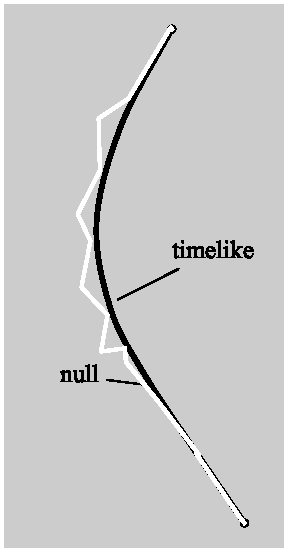
\includegraphics[width=0.72\textwidth]{fig_3.3.pdf}
\caption*{图 3.3\quad 我们总可以用一列总路径长度为零的类光路径去逼近一条类时路径。因此，类时测地线必定是固有时的极大而非极小。}
\end{figure}
现在让我们来解释前面的评注：类时测地线是固有时的极大值点。我们之所以知道这是真的，是因为给定任何一条类时曲线（无论是不是测地线），我们都能用一条类光曲线以任意精度去逼近它。为此我们要做的，只是考虑跟随这条类时曲线的“锯齿状”类光曲线，如图 3.3 所画的那样。随着我们增加尖角的数目，类光曲线越来越贴近类时曲线，而路径长度却始终为零。因此类时测地线不可能是固有时取最小值的曲线，因为它们总是无穷小地邻近于固有时更小（实际上是零）的曲线；实际上，它们使固有时取最大值。记住双生子佯谬中哪个双生子老得更多的办法就在这里——呆在家里的那个基本上处于测地线上，因此经历了更多的固有时。当然，就连这样说也有点草率；实际上，每次我们说“最大化”或“最小化”时，都应当加上修饰语“局部地”。常见的情形是：流形上两点之间不止存在一条测地线。例如，在 $S^2$ 上我们可以
过任意两点画一个大圆，并想象在两点之间旅行，既可以走短的那条路，也可以绕远走长的那条。显然两者之中一条比另一条长，尽管二者都是长度泛函的驻点。

测地线提供了一种方便的办法，把点 $p$ 的切空间 $T_p$ 映射到流形上包含 $p$ 的一个区域，这个映射叫做\textbf{指数映射}（exponential map）。这个映射反过来又为这个区域定义了一组坐标，它们自动就是 2.5 节讨论过的局部惯性坐标【点 $p$ 附近的坐标 $x^{\hat\mu}$，满足 $g_{\hat\mu\hat\nu}(p) = \eta_{\hat\mu\hat\nu}$ 且 $\partial_{\hat\sigma}g_{\hat\mu\hat\nu}(p) = 0$】。我们首先注意到，任何矢量 $k \in T_p$ 都定义了一条经过该点的唯一测地线，$k$ 是它在 $p$ 点的切矢量，且 $\lambda(p) = 0$：
\begin{equation*}
\frac{dx^\mu}{d\lambda}(\lambda = 0) = k^\mu.
\tag{3.64}
\end{equation*}
唯一性来自如下事实：测地线方程是二阶微分方程，而给定形如 $x^\mu(p)$ 和 $k^\mu = (dx^\mu/d\lambda)(p)$ 的初始数据就完全确定了一个解。在这条测地线上，$M$ 中将有唯一的一点使得 $\lambda = 1$。于是 $p$ 处的指数映射 $\exp_p : T_p \rightarrow M$ 就定义为
\begin{equation*}
\exp_p(k) = x^\nu(\lambda = 1),
\tag{3.65}
\end{equation*}
其中 $x^\nu(\lambda)$ 是在条件 (3.64) 之下测地线方程的解，如图 3.4 所示。

\begin{figure}[H]
\centering
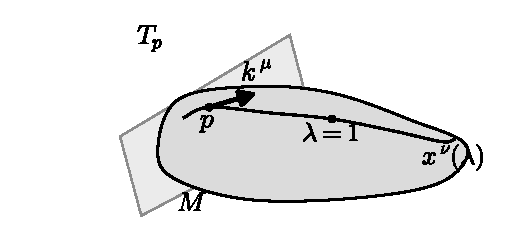
\includegraphics[width=0.72\textwidth]{fig_3.4.pdf}
\caption*{图 3.4\quad 指数映射把 $T_p$ 中的一个矢量映到 $M$ 中沿该矢量所相切的测地线上、位于单位仿射参量处的一点。}
\end{figure}
对于靠近零矢量的某组切矢量 $k^\mu$ 来说，这个映射是良好定义的，而且实际上是可逆的。不过，依赖于几何的不同，从单一点出发的不同测地线最终可能相交，在相交处 $\exp_p : T_p \rightarrow M$ 就不再一一对应。此外，指数映射的值域未必是整个流形，其定义域也未必是整个切空间。值域之所以可能不是全部 $M$，仅仅是因为可能存在两个点，它们之间没有任何测地线相连。第 8 章讨论的 anti-de Sitter 空间就是一个例子。定义域之所以可能不是全部 $T_p$，则是因为测地线可能撞上奇点——我们把奇点看作“流形的边缘”。具有此类奇点的流形被称为\textbf{测地不完备}（geodesically incomplete）的。在更仔细的讨论中，实际上应当是
反过来才对：在我们去掉了“流形的一部分被人为地手工排除”这类平凡情形之后，定义奇点的最好办法，就是把它定义为测地线看起来“终结”的地方。参见 Wald (1984) 或 Hawking and Ellis (1973)。这个问题不仅仅是技术性的；Hawking 和 Penrose 的奇点定理断言，对特定的物质内容而言，广义相对论中的时空几乎注定是测地不完备的。作为例子，广义相对论中最有用的两类时空——描写黑洞的 Schwarzschild 解和描写均匀、各向同性宇宙学的 Friedmann–Robertson–Walker 解——都具有重要的奇点；这些将在后面的章节里讨论。

现在我们用指数映射来构造局部惯性坐标。容易的部分是找出 $T_p$ 的一组基矢 $\{\hat{e}_{(\hat\mu)}\}$，使得度规的分量具有规范形式的分量：
\begin{equation*}
g_{\hat\mu\hat\nu} = g(\hat{e}_{(\hat\mu)}, \hat{e}_{(\hat\nu)}) = \eta_{\hat\mu\hat\nu}.
\tag{3.66}
\end{equation*}
这里 $g(\ ,\ )$ 表示度规，即把它看作从 $T_p \times T_p$ 到 $\mathbf{R}$ 的多重线性映射。帽子有两种不同的含义：$e$ 上面的帽子提醒我们它是基矢，而指标上面的帽子提醒我们正处于局部惯性坐标中（下面就会看到）。这一步容易，因为它不过是线性代数，还未涉及坐标；从 $g_{\mu\nu}$ 的任意一组分量出发，我们总可以把这个矩阵对角化，然后重新缩放基矢以满足式 (3.66)。我们本以为困难的部分，是找一个坐标系 $x^{\hat\mu}$，使得基矢 $\{\hat{e}_{(\hat\mu)}\}$ 恰好构成坐标基，即 $\hat{e}_{(\hat\mu)} = \partial_{\hat\mu}$，并且 $g_{\hat\mu\hat\nu}$ 的一阶偏导数为零。然而实际上，指数映射自动做到了这一点。对充分靠近 $p$ 的任何点 $q$，都存在唯一的一条测地线路径把 $p$ 与 $q$ 连接起来，以及一个唯一的参数化 $\lambda$，使得 $\lambda(p) = 0$ 且 $\lambda(q) = 1$。在 $p$ 点，这条测地线的切矢量 $k$ 可以写成我们基矢的线性组合，$k = k^{\hat\mu}\hat{e}_{(\hat\mu)}$。我们把苦苦寻找的坐标 $x^{\hat\mu}$ 就定义为这些分量：$x^{\hat\mu}(q) = k^{\hat\mu}$。换言之，我们把坐标 $x^{\hat\mu}(q)$ 定义为那个被 $\exp_p$ 映到 $q$ 的切矢量 $k$ 沿归一化基 $\{\hat{e}_{(\hat\mu)}\}$ 的分量。这样构造出来的坐标被称为 $p$ 处的\textbf{Riemann 法坐标}（Riemann normal coordinates）。

我们还须验证这些 Riemann 法坐标满足 $\partial_{\hat\sigma}g_{\hat\mu\hat\nu}(p) = 0$。注意，切空间中的一条射线（形如 $\lambda k^{\hat\mu}$ 的、参数化的矢量集合，其中 $k^{\hat\mu}$ 为某个固定矢量）经指数映射会被映成一条测地线。因此，在 Riemann 法坐标中，形如
\begin{equation*}
x^{\hat\mu}(\lambda) = \lambda k^{\hat\mu}
\tag{3.67}
\end{equation*}
的曲线将求解测地线方程。事实上，过 $p$ 的\emph{任何}测地线都可以这样表达，只要取某个合适的矢量 $k^{\hat\mu}$。于是我们有
\begin{equation*}
\frac{d^2x^{\hat\mu}}{d\lambda^2} = 0
\tag{3.68}
\end{equation*}
沿此坐标系中过 $p$ 的任何测地线都成立。但由测地线方程，我们还有
\begin{equation*}
\frac{d^2x^{\hat\mu}}{d\lambda^2}(p) = -\Gamma^{\hat\mu}_{\hat\rho\hat\sigma}(p)k^{\hat\rho}k^{\hat\sigma},
\tag{3.69}
\end{equation*}
其中 $k^{\hat\rho} = (dx^{\hat\rho}/d\lambda)(p)$。由于这对任意的 $k^{\hat\rho}$ 都成立，我们得出结论
\begin{equation*}
\Gamma^{\hat\mu}_{\hat\rho\hat\sigma}(p) = 0.
\tag{3.70}
\end{equation*}
现在用上度规相容性：
\begin{align*}
0 &= \nabla_{\hat\sigma}g_{\hat\mu\hat\nu}\\
&= \partial_{\hat\sigma}g_{\hat\mu\hat\nu} - \Gamma^{\hat\lambda}_{\hat\sigma\hat\mu}g_{\hat\lambda\hat\nu} - \Gamma^{\hat\lambda}_{\hat\sigma\hat\nu}g_{\hat\mu\hat\lambda}\\
&= \partial_{\hat\sigma}g_{\hat\mu\hat\nu},
\tag{3.71}
\end{align*}
其中所有量都在 $p$ 点取值。我们看到，Riemann 法坐标给出了 2.5 节讨论过的局部惯性坐标的一个具体实现。它们并不唯一；存在无穷多个非 Riemann 法坐标的坐标系，同样满足 $g_{\hat\mu\hat\nu}(p) = \eta_{\hat\mu\hat\nu}$ 与 $\partial_{\hat\sigma}g_{\hat\mu\hat\nu}(p) = 0$，但在围绕 $p$ 的展开中，它们与 Riemann 法坐标的差别只出现在 $x^{\hat\mu}$ 的三阶项上。

\section{再论膨胀宇宙}

让我们把目前已经发展出来的某些技术投入实用，去理解一个简单的度规。回忆第 2 章中研究过的膨胀宇宙度规：
\begin{align*}
ds^2 &= -dt^2 + a^2(t)[dx^2 + dy^2 + dz^2]\\
&= -dt^2 + a^2(t)\delta_{ij}\,dx^i dx^j.
\tag{3.72}
\end{align*}
这个度规描写了一个由平直空间截面组成的宇宙，截面随时间膨胀，固定空间坐标处的粒子之间的相对距离按尺度因子（scale factor）$a(t)$ 成比例地增长。

面对一个度规，我们做的第一件事就是计算 Christoffel 符号。正如 3.3 节末尾提到的，最容易的办法其实是显式地对形如 (3.49) 的积分作变分。把眼下考虑的度规代进去，我们得到
\begin{equation*}
I = \frac{1}{2}\int\left[-\left(\frac{dt}{d\tau}\right)^2 + a^2(t)\delta_{ij}\frac{dx^i}{d\tau}\frac{dx^j}{d\tau}\right]d\tau.
\tag{3.73}
\end{equation*}
这个技巧是考虑变分 $x^\mu \rightarrow x^\mu + \delta x^\mu$，并要求 $\delta I$ 为零。我们将在 $n$ 维流形上得到 $n$ 个方程（这里 $n = 4$），每个 $\mu$ 对应一个；每个方程都对应测地线方程的一个分量 (3.44)。在与 $x^\mu$ 相关的变分所导出的方程中，$(dx^\rho/d\tau)(dx^\sigma/d\tau)$ 的系数就是 $\Gamma^\mu_{\rho\sigma}$。

对度规 (3.72)，我们需要分别考虑对 $x^0 = t$ 的变分和对某个 $x^i$ 的变分（选哪一个都无所谓，因为各个类空方向的结果都是等价的）。让我们从 $t \rightarrow t + \delta t$ 开始。非平凡的时间依赖来自尺度因子；对它取一阶近似，
\begin{equation*}
a(t + \delta t) = a(t) + \dot{a}\,\delta t,
\tag{3.74}
\end{equation*}
其中 $\dot{a} = da/dt$。于是我们有
\begin{align*}
\delta I &= \frac{1}{2}\int\left[-2\frac{dt}{d\tau}\frac{d(\delta t)}{d\tau} + 2a\dot{a}\,\delta_{ij}\frac{dx^i}{d\tau}\frac{dx^j}{d\tau}\delta t\right]d\tau\\
&= \int\left[\frac{d^2t}{d\tau^2} + a\dot{a}\,\delta_{ij}\frac{dx^i}{d\tau}\frac{dx^j}{d\tau}\right]\delta t\,d\tau,
\tag{3.75}
\end{align*}
其中在分部积分之后我们（一如既往地）丢掉了边界项。令 $\delta t$ 的系数等于零就意味着
\begin{equation*}
\frac{d^2t}{d\tau^2} + a\dot{a}\,\delta_{ij}\frac{dx^i}{d\tau}\frac{dx^j}{d\tau} = 0,
\tag{3.76}
\end{equation*}
而它按理应当与测地线方程（取 $\mu = 0$ 时）
\begin{equation*}
\frac{d^2x^0}{d\tau^2} + \Gamma^0_{\rho\sigma}\frac{dx^\rho}{d\tau}\frac{dx^\sigma}{d\tau} = 0.
\tag{3.77}
\end{equation*}
等价。比较这两个方程就意味着
\begin{align*}
\Gamma^0_{00} &= 0,\\
\Gamma^0_{i0} = \Gamma^0_{0i} &= 0,\\
\Gamma^0_{ij} &= a\dot{a}\,\delta_{ij}.
\tag{3.78}
\end{align*}

我们可以对一个空间坐标重复这一流程：$x^i \rightarrow x^i + \delta x^i$。此时的变分便是
\begin{align*}
\delta I &= \frac{1}{2}\int a^2\left(2\delta_{ij}\frac{dx^i}{d\tau}\frac{d(\delta x^j)}{d\tau}\right)d\tau\\
&= -\int\left(a^2\frac{d^2x^i}{d\tau^2} + 2a\frac{da}{d\tau}\frac{dx^i}{d\tau}\right)\delta_{ij}\delta x^j\,d\tau.
\tag{3.79}
\end{align*}
利用链式法则，我们可以把 $da/d\tau$ 用 $\dot{a}$ 表示出来：
\begin{equation*}
\frac{da}{d\tau} = \dot{a}\frac{dt}{d\tau}.
\tag{3.80}
\end{equation*}
然后在 (3.79) 中令 $\delta x^j$ 的系数等于零，就意味着
\begin{equation*}
\frac{d^2x^i}{d\tau^2} + 2\frac{\dot{a}}{a}\frac{dt}{d\tau}\frac{dx^i}{d\tau} = 0.
\tag{3.81}
\end{equation*}
与测地线方程相比较，我们发现 Christoffel 符号必须满足
\begin{equation*}
\Gamma^i_{\rho\sigma}\frac{dx^\rho}{d\tau}\frac{dx^\sigma}{d\tau} = 2\frac{\dot{a}}{a}\frac{dt}{d\tau}\frac{dx^i}{d\tau}.
\tag{3.82}
\end{equation*}
于是，Christoffel 符号由下式给出：
\begin{align*}
\Gamma^i_{00} &= 0\\
\Gamma^i_{j0} = \Gamma^i_{0j} &= \frac{\dot{a}}{a}\delta^i_j\\
\Gamma^i_{jk} &= 0.
\tag{3.83}
\end{align*}
合在一起，(3.78) 和 (3.83) 就是度规 (3.72) 的全部联络系数。当然，无论是研究这个时空的测地线，还是计算协变导数，都需要它们；事实上，(3.76) 和 (3.81) 合起来\emph{正是}测地线方程。让我们用它来做点事情：求解类光测地线，也就是光子这类无质量粒子所走的路径——对它们我们必须用 $\lambda$ 而非 $\tau$ 作参数。不失一般性，我们可以考虑沿 $x$ 方向的路径，即 $x^\mu(\lambda) = \{t(\lambda), x(\lambda), 0, 0\}$。利用 $ds^2 = 0$，求解这类类光路径是平凡的。我们有
\begin{equation*}
0 = -dt^2 + a^2(t)dx^2,
\tag{3.84}
\end{equation*}
这意味着
\begin{equation*}
\frac{dx}{d\lambda} = \frac{1}{a}\frac{dt}{d\lambda}.
\tag{3.85}
\end{equation*}
在 2.6 节中我们曾对 $a = t^q$ 求解过它，但这里我们保持更一般的情形。另外，我们选择了考虑沿正 $x$ 方向运动的路径，这就确定了 $dx/d\lambda$ 的符号。不过，我们必须区分“类光路径”与“类光测地线”：后者是一个限制性强得多的类；要证明这些路径是测地线，我们需要把坐标 $t$ 和 $x$ 用参数 $\lambda$ 解出来。

让我们求解 $dt/d\lambda$——事后会看出，这才是我们最感兴趣的量。把类光条件 (3.85) 代入测地线方程 (3.76) 的 $\mu = 0$ 分量，并记得把 $\tau$ 换成 $\lambda$，我们得到
\begin{equation*}
\frac{d^2t}{d\lambda^2} + \frac{\dot{a}}{a}\left(\frac{dt}{d\lambda}\right)^2 = 0.
\tag{3.86}
\end{equation*}
容易验证，这个方程由下式解出：
\begin{equation*}
\frac{dt}{d\lambda} = \frac{\omega_0}{a},
\tag{3.87}
\end{equation*}
其中 $\omega_0$ 是常数。对给定的 $a(t)$，它可以立刻被积分而给出 $t(\lambda)$。但更有意思的是考虑共动观者（即固定在空间坐标处的观者）所测得的光子能量 $E$；这样的观者具有四速度
\begin{equation*}
U^\mu = (1, 0, 0, 0).
\tag{3.88}
\end{equation*}
不要被误导，以为静止粒子的四速度的类时分量总会等于 1；我们需要满足归一化条件 $g_{\mu\nu}U^\mu U^\nu = -1$，它在静止系（$U^i = 0$）中意味着 $U^0 = \sqrt{-g_{00}}$。根据式 (3.63)，并用 $p^\mu = dx^\mu/d\lambda$，我们有
\begin{align*}
E &= -p_\mu U^\mu\\
&= -g_{00}\frac{dx^0}{d\lambda}U^0\\
&= \frac{\omega_0}{a}.
\tag{3.89}
\end{align*}
现在我们明白为什么在 (3.87) 中把比例常数记作 $\omega_0$ 了：$\omega_0$ 不过是 $a = 1$ 时光子的频率。回忆 $E = \hbar\omega$，而我们使用的单位制中 $\hbar = 1$。

我们揭示了一个深刻的现象：\textbf{宇宙学红移}（cosmological redshift）。一个光子在尺度因子为 $a_1$ 处以能量 $E_1$ 被发射，而在尺度因子为 $a_2$ 处被观测到能量为 $E_2$，则有
\begin{equation*}
\frac{E_2}{E_1} = \frac{a_1}{a_2}.
\tag{3.90}
\end{equation*}
它之所以被称作“红移”，是因为光子的波长与频率成反比，而在膨胀宇宙中波长因此随时间增长。作为一个实际问题，这提供了一种测量我们与遥远星系之间尺度因子变化的简便办法，同时也可以充当距离的代理量：由于宇宙一直在单调膨胀，红移越大就意味着距离越远。按惯用记号，红移的量记为
\begin{equation*}
z = \frac{\omega_1 - \omega_2}{\omega_2} = \frac{a_2}{a_1} - 1,
\tag{3.91}
\end{equation*}
这样一来，如果从来没有过膨胀，$z$ 就为零；例如，若发射者与观者相距很近，宇宙还来不及有可察觉的膨胀，就属于这种情形。

正如 3.3 节所述，宇宙学红移\emph{不是}多普勒频移（尽管人们难免想谈论退行星系的“速度”，这是可以理解的）。现在我们可以定量地理解这个论断了。你可能会以为，就发射出的光子的行为而言，在平直时空中彼此真实地分开运动的两个星系，与在膨胀时空中固定于共动坐标上的两个星系，几乎没有什么差别。但让我们考虑一个具体的（不现实却富有教益的）例子。从平直时空出发，设想我们的两个星系起初并不彼此分开，而是静止在某个整体惯性坐标系中。一个星系朝另一个发射一个光子；在光子旅行的途中，我们迅速把两个星系拉开，直到它们的间距变为原来的两倍，然后让它们静止在那个距离上；随后光子被第二个星系吸收。显然不会有任何多普勒频移，因为两个星系在发射和吸收时都是静止的。现在考虑膨胀时空中的类似现象，星系钉在固定的共动坐标上。开始时尺度因子恒定（宇宙不膨胀）。一个星系发出一个光子，我们设想在光子旅行的过程中宇宙开始膨胀，直到尺度因子变为原来的两倍，然后在光子被吸收之前停止膨胀。在这种情形下肯定会有红移，尽管在发射和吸收时都不存在任何“相对运动”（这个概念反正也是定义不良的）；光子的波长会随着尺度因子翻倍而翻倍，于是我们观测到红移 $z = 1$。这个例子演示了宇宙学红移与常规多普勒效应之间的概念区别。

在测地线方程之外，协变导数还将在另一项任务中发挥作用：把物理定律从狭义相对论的平直时空推广到广义相对论的弯曲几何。正如我们在下一章会更详细讨论的，一条简单的经验法则是：把所有偏导数都换成协变导数，把平直时空度规 $\eta_{\mu\nu}$ 出现的所有地方都换成弯曲度规 $g_{\mu\nu}$。例如，狭义相对论的能量-动量守恒方程 $\partial_\mu T^{\mu\nu} = 0$（其中 $T^{\mu\nu}$ 是能量-动量张量）就变成
\begin{equation*}
\nabla_\mu T^{\mu\nu} = 0.
\tag{3.92}
\end{equation*}
在宇宙学中，我们通常把充满宇宙的物质建模为理想流体；相应的能量-动量张量来自把式 (1.114) 推广到弯曲时空：
\begin{equation*}
T^{\mu\nu} = (\rho + p)U^\mu U^\nu + pg^{\mu\nu}.
\tag{3.93}
\end{equation*}
回忆一下，$\rho$ 是能量密度，$p$ 是压强，而 $U^\mu$ 是流体的四速度。对度规 (3.72) 而言，逆度规的分量为
\begin{equation*}
g^{\mu\nu} = \begin{pmatrix} -1 & & & \\ & a^{-2} & & \\ & & a^{-2} & \\ & & & a^{-2} \end{pmatrix}.
\tag{3.94}
\end{equation*}

在这些坐标中，我们可以取流体处于其静止系，于是四速度的分量为 $U^\mu = (1, 0, 0, 0)$。事实上，正如我们以后会看到的，要让这个特定的度规求解 Einstein 方程，流体就必须处于其静止系。于是能量-动量张量取如下形式：
\begin{equation*}
T^{\mu\nu} = \begin{pmatrix} \rho & & & \\ & a^{-2}p & & \\ & & a^{-2}p & \\ & & & a^{-2}p \end{pmatrix}.
\tag{3.95}
\end{equation*}
注意，这些分量是专就度规 (3.72) 而言的；对其他度规，它们一般看起来会不同。

让我们看看能量-动量守恒方程 $\nabla_\mu T^{\mu\nu} = 0$ 对膨胀宇宙中的理想流体意味着什么。协变导数的法则 (3.17) 给出
\begin{equation*}
\nabla_\mu T^{\mu\nu} = \partial_\mu T^{\mu\nu} + \Gamma^\mu_{\mu\lambda}T^{\lambda\nu} + \Gamma^\nu_{\mu\lambda}T^{\mu\lambda} = 0.
\tag{3.96}
\end{equation*}
这个方程有四个分量，每个 $\nu$ 对应一个，尽管 $\nu = i \in \{1, 2, 3\}$ 的三个分量彼此等价。（译注：原文此处两处印作 $\mu$。）让我们先逐项考察 $\nu = 0$ 的分量。第一项是直截了当的：
\begin{equation*}
\partial_\mu T^{\mu 0} = \partial_0 T^{00} = \dot{\rho}.
\tag{3.97}
\end{equation*}
第二项是
\begin{equation*}
\Gamma^\mu_{\mu\lambda}T^{\lambda 0} = \Gamma^\mu_{\mu 0}T^{00} = 3\frac{\dot{a}}{a}\rho,
\tag{3.98}
\end{equation*}
第三项是
\begin{equation*}
\Gamma^0_{\mu\lambda}T^{\mu\lambda} = \Gamma^0_{00}T^{00} + \Gamma^0_{11}T^{11} + \Gamma^0_{22}T^{22} + \Gamma^0_{33}T^{33} = 3\frac{\dot{a}}{a}p.
\tag{3.99}
\end{equation*}
在上面每一组等式里，我们都先利用了 $T^{\mu\nu}$ 是对角的事实，然后代入了这个度规下能量-动量张量与联络系数的显式公式。合在一起，我们便得到
\begin{equation*}
\dot{\rho} = -3\frac{\dot{a}}{a}(\rho + p).
\tag{3.100}
\end{equation*}
现在让我们看某个空间分量，为明确起见取 $\nu = 1$。再次逐项计算，式 (3.96) 中的第一项为
\begin{equation*}
\partial_\mu T^{\mu 1} = \partial_1 T^{11} = a^{-2}\partial_x p.
\tag{3.101}
\end{equation*}
第二项和第三项是
\begin{equation*}
\Gamma^\mu_{\mu\lambda}T^{\lambda 1} = \Gamma^\mu_{\mu 1}T^{11} = 0,
\tag{3.102}
\end{equation*}
以及
\begin{equation*}
\Gamma^1_{\mu\lambda} T^{\mu\lambda} = \Gamma^1_{00} T^{00} + \Gamma^1_{11} T^{11} + \Gamma^1_{22} T^{22} + \Gamma^1_{33} T^{33} = 0. \tag{3.103}
\end{equation*}

对 $\nu=2$ 和 $\nu=3$ 也会得到等价的结果。于是，能量-动量守恒方程的空间分量简单地化为

\begin{equation*}
\partial_i p = 0. \tag{3.104}
\end{equation*}

把这些结果与我们在 Minkowski 时空中会得到的结果作比较是很有启发性的，后者只需令 $a=1$、$\dot a =0$ 即可得到。压强梯度方程 (3.104) 不受影响，所以曲率对空间分量没有影响：对于一个在共动观者看来静止的流体，压强必须在整个空间中为常数。而时间分量则不同：宇宙的膨胀给 (3.100) 的右端引入了一个非零的项。为了理解这个新特点的后果，让我们考虑如下形式的物态方程

\begin{equation*}
p = w\rho, \tag{3.105}
\end{equation*}

其中 $w$ 是某个常数。那么 (3.100) 变为

\begin{equation*}
\frac{\dot\rho}{\rho} = -3(1+w)\frac{\dot a}{a}, \tag{3.106}
\end{equation*}

求解可得

\begin{equation*}
\rho \propto a^{-3(1+w)}. \tag{3.107}
\end{equation*}

在第 1 章中我们提到过三种物态方程形如 (3.105) 的理想流体：尘埃，$w=0$；辐射，$w=1/3$；以及真空，$w=-1$。一组非相对论性、无相互作用的粒子表现得像尘埃；一组光子或其他无质量粒子表现得像辐射；而遍布时空的非零常数能量密度则表现得像真空。由 (3.107) 我们看到，物态方程决定了能量密度随宇宙膨胀的演化方式：

\begin{align*}
\text{物质}\quad & p = 0 & \rho &\propto a^{-3}\\
\text{辐射}\quad & p = \tfrac{1}{3}\rho & \rho &\propto a^{-4}\\
\text{真空}\quad & p = -\rho & \rho &= \text{常数}. \tag{3.108}
\end{align*}

我们将在第 8 章更深入地探讨这些行为；现在只须注意它们是合理的。对尘埃而言，能量密度来自每个粒子的静止质量；如果所有粒子都具有质量 $m$，能量密度就是 $\rho = nm$，其中 $n$ 是数密度（number density）。由于数密度按 $a^{-3}$ 下降（共动区域的物理体积增大，而粒子总数保持不变），同时质量不变，我们预期能量密度满足 $\rho \propto a^{-3}$。对辐射而言，每个粒子（比如光子）的能量随宇宙膨胀按 $a^{-1}$ 红移掉；由于数密度仍满足 $n \propto a^{-3}$，我们预期 $\rho \propto a^{-4}$。最后，真空能量密度是任一物理体积中固有的、不随时间改变的能量；它在宇宙膨胀时完全不红移，所以我们得到 $\rho = \text{常数}$。

这个例子生动地展现了平直时空与弯曲时空之间的差异。例如，考虑一下我们可能禁不住想称之为“能量”的东西，即能量密度对空间的积分：$E = \int \rho a^3\, d^3x$，其中边界取在固定的共动坐标处，因此该区域随宇宙一起膨胀，而因子 $a^3$ 来自空间度规 $a^2\delta_{ij}$ 的行列式的平方根。这个量一般而言显然不守恒。对尘埃，由于 $\rho \propto a^{-3}$，$E$ 在宇宙膨胀时保持不变；但对辐射它不断减小，而对真空能量它不断增大。这令人沮丧，因为能量守恒是物理学中最受珍视的原理之一。发生了什么？一种思考方式是从诺特定理（Noether's theorem）出发，该定理指出每一种对称性都蕴含一个守恒量。能量正是由时间平移不变性导出的守恒量。显然，在膨胀宇宙中，能量-动量张量定义在一个随时间变化的背景上；因此没有理由相信能量应当守恒。（用 3.8 节将要引入的语言来说，就是“不存在类时 Killing 矢量”。）尽管如此，我们仍继续把 $\nabla_\mu T^{\mu\nu} = 0$ 称为能量-动量守恒方程。它传达的观念是：能量-动量张量服从一条确定的定律，即使不存在与守恒能量相对应的积分。从平直时空到弯曲时空的转变引入了 (3.96) 中额外的 Christoffel 符号项；粗略地说，这些项的作用是允许能量在物质场（即 $T^{\mu\nu}$）与引力场之间转移。然而这个说法并不十分正式，你也不要把它推得太远——事实证明，很难给引力场联系上一个局域的能量密度，尽管在某些情形下这是可能的。

当然，还有一种时间平移不变性的概念，它指的不是背景时空，而是理论本身（也就是说，指的是定义理论的方程，而不是理论的某个具体解）。我们尚未建立起广义相对论的动力学方程，但它们将被证明在时间平移下不变，而且在任何其他类型的坐标变换下也不变——它们本来就必须如此。这种广义坐标不变性给理论的允许组态加上了一组约束，而且通常需要更精细的分析来处理。

最后，你应当接受这样一点：平直时空与弯曲时空之间存在着深刻的差异，我们来自平直时空物理学的一些心仪观念，在这个更一般的框架中将被大幅修正。这并不是广义相对论有什么缺陷的信号，而是抛弃我们习以为常的刚性时空几何之后的一个自然结果。

\section{Riemann 曲率张量}

在建立了协变导数和平行移动这套机制之后，我们终于准备好正面对待曲率了。曲率由 Riemann 张量来量化，而 Riemann 张量由联络导出。这种曲率量度背后的想法是：我们知道联络的“平直性”是什么意思——与欧几里得型或 Minkowski 型度规相联系的常规（且通常是隐含的）Christoffel 联络具有若干性质，它们可以被看作平直性的不同表现。这包括：沿闭合回路一周的平行移动不改变矢量；张量的协变导数相互对易；初始平行的测地线保持平行。正如我们将看到的，当我们研究这些性质在更一般的情形下如何被改变时，Riemann 张量就出现了。

我们前面已经论证过（以二维球面为例），在弯曲空间中沿闭合回路一周的平行移动会导致矢量发生一个变换。所得的变换依赖于回路所包围的总曲率；更有用的应当是每一点曲率的局域描述，而这正是 Riemann 张量所要提供的。因此，引入 Riemann 张量的一种常规做法是考虑绕无穷小回路的平行移动。这里我们不打算那样做，而是采取一条更直接的路线。不过，即使不细究细节，也能够看出答案应当取什么形式。由于时空在足够小的区域内看起来是平直的，我们的回路将由两个（无穷小的）矢量 $A^\mu$ 和 $B^\nu$ 确定。我们想象把矢量 $V^\mu$ 平行移动：先沿 $A^\mu$ 的方向移动，再沿 $B^\nu$，然后沿 $A^\mu$ 和 $B^\nu$ 逆向退回出发点，如图 3.5 所示。

\begin{figure}[H]
\centering
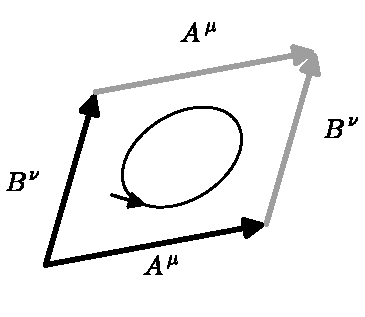
\includegraphics[width=0.72\textwidth]{fig_3.5.pdf}
\caption*{图 3.5\quad 由两个矢量 $A^\mu$ 与 $B^\nu$ 定义的无穷小回路}
\end{figure}

我们知道平行移动的作用与坐标无关，所以应当存在某个张量，它告诉我们当矢量回到出发点时发生了怎样的变化；它是作用在矢量上的一个线性变换，因而含有一个上指标和一个下指标。但它还依赖于定义回路的两个矢量 $A$ 和 $B$；因此还应当有两个附加的下指标，用来与 $A^\mu$ 和 $B^\nu$ 缩并。此外，这个张量在这两个指标上应当是反对称的，因为交换这两个矢量相当于沿相反方向绕行回路，应当给出原答案的逆。这与“若 $A$ 与 $B$ 是同一个矢量则变换应为零”的事实一致。于是我们预期，这个矢量绕回路平行移动一周所经历的改变 $\delta V^\rho$ 应当具有如下形式

\begin{equation*}
\delta V^\rho = R^\rho{}_{\sigma\mu\nu} V^\sigma A^\mu B^\nu, \tag{3.109}
\end{equation*}

其中 $R^\rho{}_{\sigma\mu\nu}$ 是一个 $(1,3)$ 型张量，称为 \textbf{Riemann 张量}（Riemann tensor，或简称曲率张量）。它在后两个指标上反对称：

\begin{equation*}
R^\rho{}_{\sigma\mu\nu} = -R^\rho{}_{\sigma\nu\mu}. \tag{3.110}
\end{equation*}

当然，如果把 (3.109) 取作 Riemann 张量的定义，就需要为指标的排列顺序选定一个约定。关于这个约定应当是什么，完全没有共识，所以要当心。

基于我们对平行移动的了解，本可以非常仔细地完成必要的操作，看看矢量在这一操作下会发生什么，其结果将是一个用联络系数表示的曲率张量公式。然而，快得多的办法是考虑一个相关的操作，即两个协变导数的对易子。它与绕回路平行移动之间的关系应当一目了然：张量沿某一方向的协变导数量度的是，该张量相对于它被平行移动时应有的样子变化了多少，因为张量沿它被平行移动的那个方向的协变导数为零。于是，两个协变导数的对易子量度的就是“先把张量沿一个方向平行移动、再沿另一个方向”与“次序相反”这两种做法之间的差别，如图 3.6 所示。

\begin{figure}[H]
\centering
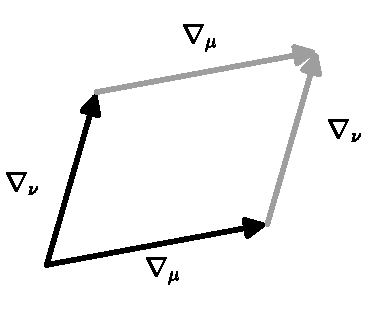
\includegraphics[width=0.72\textwidth]{fig_3.6.pdf}
\caption*{图 3.6\quad 两个协变导数的对易子}
\end{figure}

实际计算非常直接。考虑矢量场 $V^\rho$，我们取

\begin{align*}
[\nabla_\mu, \nabla_\nu] V^\rho &= \nabla_\mu\nabla_\nu V^\rho - \nabla_\nu\nabla_\mu V^\rho\\
&= \partial_\mu(\nabla_\nu V^\rho) - \Gamma^\lambda_{\mu\nu}\nabla_\lambda V^\rho + \Gamma^\rho_{\mu\sigma}\nabla_\nu V^\sigma - (\mu \leftrightarrow \nu)\\
&= \partial_\mu\partial_\nu V^\rho + (\partial_\mu\Gamma^\rho_{\nu\sigma})V^\sigma + \Gamma^\rho_{\nu\sigma}\partial_\mu V^\sigma - \Gamma^\lambda_{\mu\nu}\partial_\lambda V^\rho - \Gamma^\lambda_{\mu\nu}\Gamma^\rho_{\lambda\sigma}V^\sigma\\
&\quad + \Gamma^\rho_{\mu\sigma}\partial_\nu V^\sigma + \Gamma^\rho_{\mu\sigma}\Gamma^\sigma_{\nu\lambda}V^\lambda - (\mu \leftrightarrow \nu)\\
&= (\partial_\mu\Gamma^\rho_{\nu\sigma} - \partial_\nu\Gamma^\rho_{\mu\sigma} + \Gamma^\rho_{\mu\lambda}\Gamma^\lambda_{\nu\sigma} - \Gamma^\rho_{\nu\lambda}\Gamma^\lambda_{\mu\sigma})V^\sigma - 2\Gamma^\lambda_{[\mu\nu]}\nabla_\lambda V^\rho. \tag{3.111}
\end{align*}

在最后一步中，我们对一些哑指标做了改名，并删去了反对称化后相消的一些项。我们认出，最后一项中被反对称化的联络系数恰好是挠率张量的一半，而左端显然是张量；因此括号中的表达式本身必定是张量。我们写成

\begin{equation*}
[\nabla_\mu, \nabla_\nu] V^\rho = R^\rho{}_{\sigma\mu\nu}V^\sigma - T^\lambda{}_{\mu\nu}\nabla_\lambda V^\rho, \tag{3.112}
\end{equation*}

其中 Riemann 张量被确认为

\begin{equation*}
R^\rho{}_{\sigma\mu\nu} = \partial_\mu\Gamma^\rho_{\nu\sigma} - \partial_\nu\Gamma^\rho_{\mu\sigma} + \Gamma^\rho_{\mu\lambda}\Gamma^\lambda_{\nu\sigma} - \Gamma^\rho_{\nu\lambda}\Gamma^\lambda_{\mu\sigma}. \tag{3.113}
\end{equation*}

关于这个表达式的推导，有几点值得注意：

\begin{itemize}
\item 当然，我们并没有证明 (3.113) 与 (3.109) 中出现的确实是同一个张量，但事实上确实如此。习题中会请你证明这一点。
\item 或许令人惊讶的是，对易子 $[\nabla_\mu, \nabla_\nu]$ 虽然看似一个微分算符，但它作用在矢量场上的效果（至少在没有挠率时）是一个简单的乘法变换。Riemann 张量量度的是协变导数对易子中正比于矢量场的那一部分，而挠率张量量度的是正比于矢量场的协变导数的那一部分；二阶导数完全没有出现。
\item 注意 (3.113) 是由非张量性的元素构造出来的；你可以验证，各个变换定律恰好都行得通，使这个特定的组合成为一个合法的张量。
\item $R^\rho{}_{\sigma\mu\nu}$ 在其最后两个指标上的反对称性可以直接从这个公式及其推导看出。
\item 我们完全由联络构造了曲率张量（完全没有提及度规）。我们足够小心，因此上面的表达式对任何联络都成立，无论它是否度规相容或无挠。
\item 用我们如今已惯用的方法，可以计算出 $[\nabla_\rho, \nabla_\sigma]$ 作用在任意阶张量上的结果。答案是
\begin{align*}
[\nabla_\rho, \nabla_\sigma] X^{\mu_1\cdots\mu_k}{}_{\nu_1\cdots\nu_\ell}
&= -T^\lambda{}_{\rho\sigma}\nabla_\lambda X^{\mu_1\cdots\mu_k}{}_{\nu_1\cdots\nu_\ell}\\
&\quad + R^{\mu_1}{}_{\lambda\rho\sigma}X^{\lambda\mu_2\cdots\mu_k}{}_{\nu_1\cdots\nu_\ell} + R^{\mu_2}{}_{\lambda\rho\sigma}X^{\mu_1\lambda\cdots\mu_k}{}_{\nu_1\cdots\nu_\ell} + \cdots\\
&\quad - R^\lambda{}_{\nu_1\rho\sigma}X^{\mu_1\cdots\mu_k}{}_{\lambda\nu_2\cdots\nu_\ell} - R^\lambda{}_{\nu_2\rho\sigma}X^{\mu_1\cdots\mu_k}{}_{\nu_1\lambda\cdots\nu_\ell} - \cdots. \tag{3.114}
\end{align*}
\end{itemize}

挠率张量与 Riemann 张量都可以看作多重线性映射，用矢量场对易子可以把它们表达得十分优雅。把挠率看作从两个矢量场到第三个矢量场的映射，我们有

\begin{equation*}
T(X, Y) = \nabla_X Y - \nabla_Y X - [X, Y], \tag{3.115}
\end{equation*}

而把 Riemann 张量看作从三个矢量场到第四个矢量场的映射，我们有（这套记号看上去有点怪，但它是标准的）

\begin{equation*}
R(X, Y)Z = \nabla_X\nabla_Y Z - \nabla_Y\nabla_X Z - \nabla_{[X, Y]}Z. \tag{3.116}
\end{equation*}

在这些表达式中，记号 $\nabla_X$ 指沿矢量场 $X$ 的协变导数；用分量写即 $\nabla_X = X^\mu\nabla_\mu$。举例来说，(3.116) 等价于

\begin{align*}
R^\rho{}_{\sigma\mu\nu} X^\mu Y^\nu Z^\sigma &= X^\lambda\nabla_\lambda(Y^\eta\nabla_\eta Z^\rho) - Y^\lambda\nabla_\lambda(X^\eta\nabla_\eta Z^\rho)\\
&\quad - (X^\lambda\partial_\lambda Y^\eta - Y^\lambda\partial_\lambda X^\eta)\nabla_\eta Z^\rho, \tag{3.117}
\end{align*}

你可以验证它与 (3.113) 等价。注意 (3.116) 中的两个矢量 $X$ 和 $Y$ 对应于 Riemann 张量分量形式中的最后两个指标。(3.116) 中含对易子 $[X, Y]$ 的最后一项，在 $X$ 和 $Y$ 取坐标基矢量场时为零（因为 $[\partial_\mu, \partial_\nu] = 0$），这正是我们当初计算两个协变导数的对易子时这一项没有出现的原因。我们不会大量使用这套记号，但你可能会在文献中遇到它，所以应当能够解读它。

在把曲率张量定义为刻画联络的量之后，现在应当承认：在广义相对论中我们最关心的是 Christoffel 联络。此时联络由度规导出，相应的曲率可以视为度规本身的曲率。这一对应使我们终于能够理解那个非正式的观念：度规看起来是欧几里得型或 Minkowski 型的空间是平直的。事实上，这在两个方向上都成立：

\begin{itemize}
\item 如果存在一个坐标系，其中度规的分量是常数，那么 Riemann 张量将为零。
\item 如果 Riemann 张量为零，我们总可以构造一个坐标系，使度规分量是常数。
\end{itemize}

严格说来，这些论断应当限制在流形的单连通（simply-connected）区域上（区域内的所有回路都能在不离开该区域的前提下光滑地形变为一点）；下面我们将默认这个条件。

第一条很容易证明。如果我们所在的坐标系使 $\partial_\sigma g_{\mu\nu} = 0$ 处处成立，而不仅仅在一点成立，那么 $\Gamma^\lambda_{\mu\nu} = 0$ 且 $\partial_\sigma\Gamma^\lambda_{\mu\nu} = 0$；于是由 (3.113) 得 $R^\rho{}_{\sigma\mu\nu} = 0$。但这是张量方程，只要它在某个坐标系中成立，它在任何坐标系中都必然成立。因此，“Riemann 张量为零”是“有可能找到使 $g_{\mu\nu}$ 的分量处处为常数的坐标”的必要条件。

第二个论断——$R^\rho{}_{\sigma\mu\nu} = 0$ 处处成立蕴含我们能找到一个使度规分量处处为常数的坐标系——证明起来更难（但也难不到哪里去）。作为热身，考虑在某点 $p$ 定义的一个 1-形式 $\omega = \omega_\mu dx^\mu$。对每条包含 $p$ 的路径 $x^\mu(\lambda)$，只要要求 $\omega_\mu$ 被平行移动，我们就能沿该路径构造一个唯一的 1-形式场：

\begin{equation*}
\frac{dx^\mu}{d\lambda}\nabla_\mu\omega_\nu = 0. \tag{3.118}
\end{equation*}

一般而言，如果我们对从 $p$ 出发、经过另一点 $q$ 的不同路径执行这一步骤，$\omega_\mu$ 在 $q$ 处的值将依赖于路径。然而，若 Riemann 张量处处为零，平行移动便与路径无关，我们就能在整个流形上定义一个唯一的 1-形式场。因此 (3.118) 必须对任意的 $dx^\mu/d\lambda$ 都成立；这只有在 $\omega_\mu$ 为协变常数时才可能：

\begin{equation*}
\nabla_\mu\omega_\nu = 0. \tag{3.119}
\end{equation*}

在任意流形上这个方程一般无解；它在这里有解，只是因为我们假设了曲率为零。我们可以取 (3.119) 的反对称部分，而由 (3.36) 可知这正是外微分：

\begin{equation*}
\nabla_{[\mu}\omega_{\nu]} = \partial_{[\mu}\omega_{\nu]} = 0, \tag{3.120}
\end{equation*}

或者，用无指标记号写成

\begin{equation*}
d\omega = 0. \tag{3.121}
\end{equation*}

换言之，$\omega$ 是闭的。它同时也是恰当的（存在一个标量函数 $\alpha$ 使得 $\omega = d\alpha$），因为我们已经限制了所工作区域的拓扑。用分量表示即

\begin{equation*}
\omega_\mu = \partial_\mu\alpha. \tag{3.122}
\end{equation*}

1-形式 $\omega$ 并没有任何特殊之处，所以我们可以在 $n$ 维流形上用一组 1-形式 $\hat\theta^{(a)}$（其中 $a \in \{1 \ldots n\}$）重复这一步骤。我们可以选取这组 1-形式，使它们构成对偶空间 $T^*_p$ 的一个归一化基，使得度规相对于这组基的分量就是规范形式的分量；换句话说，

\begin{equation*}
ds^2(p) = \eta_{ab}\, \hat\theta^{(a)}\otimes\hat\theta^{(b)}. \tag{3.123}
\end{equation*}

这里我们在广义的意义上使用 $\eta_{ab}$：一个对角元各自为 $+1$ 或 $-1$、其余元素为零的矩阵。$+1$ 与 $-1$ 的具体排列取决于度规的规范形式，但与当前的论证无关。现在让我们把整组基 1-形式平行移动到流形各处；Riemann 张量的消失保证了结果与所走的路径无关。由于相对于度规相容的联络，度规总是被自动地平行移动，度规分量将保持不变，

\begin{equation*}
ds^2(\text{任何地方}) = \eta_{ab}\, \hat\theta^{(a)}\otimes\hat\theta^{(b)}. \tag{3.124}
\end{equation*}

于是我们指定了一组 1-形式场，它们处处定义了一个使度规分量为常数的基。这完全没有什么了不起；无论曲率是多少，在任何流形上都能做到。我们想要表明的是，这是一个\emph{坐标}基（只有当曲率消失时这才可能）。然而，用导出 (3.122) 的同样论证可以知道，所有 $\hat\theta^{(a)}$ 都是恰当形式，因此存在一组函数 $y^a$，使这些 1-形式场是它们的梯度，

\begin{equation*}
\hat\theta^{(a)} = dy^a. \tag{3.125}
\end{equation*}

这 $n$ 个函数正是我们寻求的坐标；在整个流形上，度规取如下形式

\begin{equation*}
ds^2 = \eta_{ab}\, dy^a dy^b. \tag{3.126}
\end{equation*}

到了这里，如果你愿意，尽可以把指标从 $a$、$b$ 换回 $\mu$、$\nu$。

这样我们就验证了：Riemann 张量为我们提供了一个判据，可以回答“某个面目可憎的度规是否其实是别扭坐标系中平直空间的度规”这个问题。如果我们算出这种度规的 Riemann 张量并发现它为零，就知道度规是平直的；若它不为零，就存在曲率。

\section{Riemann 张量的性质}

Riemann 张量有四个指标，在 $n$ 维空间中天真地数有 $n^4$ 个独立分量。实际上，反对称性质 (3.110) 意味着这最后两个指标只能取 $n(n-1)/2$ 个独立值，于是剩下 $n^3(n-1)/2$ 个独立分量。然而当我们考虑 Christoffel 联络时，另外一些对称性会把独立分量的数目进一步削减。现在就来考察这些对称性。

推导这些附加对称性的最简单办法，是考察全下标形式的 Riemann 张量

\begin{equation*}
R_{\rho\sigma\mu\nu} = g_{\rho\lambda}R^\lambda{}_{\sigma\mu\nu}. \tag{3.127}
\end{equation*}

让我们进一步考虑这个张量在点 $p$ 处建立的局部惯性坐标 $x^{\hat\mu}$ 中的分量。此时 Christoffel 符号本身将为零，但它们的导数不为零。于是我们有

\begin{align*}
R_{\hat\rho\hat\sigma\hat\mu\hat\nu}(p) &= g_{\hat\rho\hat\lambda}\big(\partial_{\hat\mu}\Gamma^{\hat\lambda}{}_{\hat\nu\hat\sigma} - \partial_{\hat\nu}\Gamma^{\hat\lambda}{}_{\hat\mu\hat\sigma}\big)\\
&= \tfrac{1}{2} g_{\hat\rho\hat\lambda} g^{\hat\lambda\hat\tau}\big(\partial_{\hat\mu}\partial_{\hat\nu}g_{\hat\sigma\hat\tau} + \partial_{\hat\mu}\partial_{\hat\sigma}g_{\hat\tau\hat\nu} - \partial_{\hat\mu}\partial_{\hat\tau}g_{\hat\nu\hat\sigma} - \partial_{\hat\nu}\partial_{\hat\mu}g_{\hat\sigma\hat\tau}\\
&\quad - \partial_{\hat\nu}\partial_{\hat\sigma}g_{\hat\tau\hat\mu} + \partial_{\hat\nu}\partial_{\hat\tau}g_{\hat\mu\hat\sigma}\big)\\
&= \tfrac{1}{2}\big(\partial_{\hat\mu}\partial_{\hat\sigma}g_{\hat\rho\hat\nu} - \partial_{\hat\mu}\partial_{\hat\rho}g_{\hat\nu\hat\sigma} - \partial_{\hat\nu}\partial_{\hat\sigma}g_{\hat\rho\hat\mu} + \partial_{\hat\nu}\partial_{\hat\rho}g_{\hat\mu\hat\sigma}\big). \tag{3.128}
\end{align*}

第一行我们用了 $\Gamma^{\hat\tau}{}_{\hat\mu\hat\nu}(p) = 0$，第二行用了 Riemann 法坐标（Riemann normal coordinates）中的 $\partial_{\hat\mu}g^{\hat\lambda\hat\tau} = 0$，第三行则用了偏导数可对易这一事实。从这个表达式出发，我们可以立刻注意到 $R_{\rho\sigma\mu\nu}$ 的三个性质：它在头两个指标上反对称，

\begin{equation*}
R_{\rho\sigma\mu\nu} = -R_{\sigma\rho\mu\nu}, \tag{3.129}
\end{equation*}

在后两个指标上反对称［这一点我们已经从 (3.110) 知道了］，

\begin{equation*}
R_{\rho\sigma\mu\nu} = -R_{\rho\sigma\nu\mu}, \tag{3.130}
\end{equation*}

并且把头一对指标与后一对指标互换时它不变：

\begin{equation*}
R_{\rho\sigma\mu\nu} = R_{\mu\nu\rho\sigma}. \tag{3.131}
\end{equation*}

稍微再多做一点工作（细节留给你想象），可以看出最后三个指标的循环置换（cyclic permutations）之和为零：

\begin{equation*}
R_{\rho\sigma\mu\nu} + R_{\rho\mu\nu\sigma} + R_{\rho\nu\sigma\mu} = 0. \tag{3.132}
\end{equation*}

给定 (3.130)，容易看出这最后一条性质等价于最后三个指标的反对称部分为零：

\begin{equation*}
R_{\rho[\sigma\mu\nu]} = 0. \tag{3.133}
\end{equation*}

所有这些性质都是在特殊坐标系中导出的，但它们都是张量方程，因此在任何坐标中都成立（所以我们也就懒得给指标加帽子了）。它们并非全都独立；只要花些功夫，你可以证明 (3.129)、(3.130) 和 (3.133) 合起来蕴含 (3.131)。这些方程之间的逻辑依存关系，通常不如“它们为真”这一事实来得重要。

知道了 Riemann 张量不同分量之间的这些关系，还剩下多少个独立的量？让我们从如下事实出发：$R_{\rho\sigma\mu\nu}$ 在头两个指标上反对称，在后两个指标上反对称，并且交换这两对指标时对称。这意味着我们可以把它看作对称矩阵 $R_{[\rho\sigma][\mu\nu]}$，其中指标对 $\rho\sigma$ 和 $\mu\nu$ 被当作单个指标。一个 $m\times m$ 对称矩阵有 $m(m+1)/2$ 个独立分量，而一个 $n\times n$ 反对称矩阵有 $n(n-1)/2$ 个独立分量。于是我们得到

\begin{equation*}
\tfrac{1}{2}\Big[\tfrac{1}{2}n(n-1)\Big]\Big[\tfrac{1}{2}n(n-1)+1\Big] = \tfrac{1}{8}\big(n^4 - 2n^3 + 3n^2 - 2n\big) \tag{3.134}
\end{equation*}

个独立分量。我们还必须处理附加的对称性 (3.133)。(3.133) 的一个直接推论是，Riemann 张量的全反对称（totally antisymmetric）部分为零，

\begin{equation*}
R_{[\rho\sigma\mu\nu]} = 0. \tag{3.135}
\end{equation*}

事实上，这个方程再加上其他对称性 (3.129)、(3.130) 和 (3.131)，就足以蕴含 (3.133)；只需展开 (3.135) 并处理所得各项即可轻易证明。因此，一旦其他对称性都已计入，附加约束 (3.135) 就等价于 (3.133)。这代表多少个独立的限制？让我们设想分解

\begin{equation*}
R_{\rho\sigma\mu\nu} = X_{\rho\sigma\mu\nu} + R_{[\rho\sigma\mu\nu]}. \tag{3.136}
\end{equation*}

容易看出，任何全反对称的 4 指标张量都自动在其第一个和最后一个指标上反对称，并且在两对指标互换下对称。因此这些性质是对 $X_{\rho\sigma\mu\nu}$ 的独立限制，与要求 (3.135) 无关。一个全反对称的 4 指标张量有 $n(n-1)(n-2)(n-3)/4!$ 项，因此 (3.135) 把独立分量的数目削减了这么多。剩下

\begin{equation*}
\tfrac{1}{8}\big(n^4 - 2n^3 + 3n^2 - 2n\big) - \tfrac{1}{24}n(n-1)(n-2)(n-3) = \tfrac{1}{12}n^2\big(n^2 - 1\big) \tag{3.137}
\end{equation*}

个独立的 Riemann 张量分量。

因此在四维情形，Riemann 张量有 20 个独立分量。（在一维时它一个也没有。）这二十个函数恰好对应我们在第 2 章初次讨论局部惯性坐标时、无法靠巧妙选取坐标而消去的度规二阶导数的 20 个自由度。这应当会增强你的信心：Riemann 张量是曲率的恰当量度。

除了 Riemann 张量的代数对称性（它们约束任一点上独立分量的数目）之外，它还服从一个微分恒等式，约束它在不同点上的相对取值。考虑 Riemann 张量的协变导数，在局部惯性坐标中取值：

\begin{align*}
\nabla_{\hat\lambda}R_{\hat\rho\hat\sigma\hat\mu\hat\nu} &= \partial_{\hat\lambda}R_{\hat\rho\hat\sigma\hat\mu\hat\nu}\\
&= \tfrac{1}{2}\partial_{\hat\lambda}\big(\partial_{\hat\mu}\partial_{\hat\sigma}g_{\hat\rho\hat\nu} - \partial_{\hat\mu}\partial_{\hat\rho}g_{\hat\nu\hat\sigma} - \partial_{\hat\nu}\partial_{\hat\sigma}g_{\hat\rho\hat\mu} + \partial_{\hat\nu}\partial_{\hat\rho}g_{\hat\mu\hat\sigma}\big). \tag{3.138}
\end{align*}

对一个只在一点成立的表达式求导似乎不合规则，但我们忽略掉的项全都正比于 $\partial_{\hat\sigma}g_{\hat\mu\hat\nu}$，因而为零。我们想考虑头三个指标的循环置换之和：

\begin{align*}
&\nabla_{\hat\lambda}R_{\hat\rho\hat\sigma\hat\mu\hat\nu} + \nabla_{\hat\rho}R_{\hat\sigma\hat\lambda\hat\mu\hat\nu} + \nabla_{\hat\sigma}R_{\hat\lambda\hat\rho\hat\mu\hat\nu}\\
&= \tfrac{1}{2}\big(\partial_{\hat\lambda}\partial_{\hat\mu}\partial_{\hat\sigma}g_{\hat\rho\hat\nu} - \partial_{\hat\lambda}\partial_{\hat\mu}\partial_{\hat\rho}g_{\hat\nu\hat\sigma} - \partial_{\hat\lambda}\partial_{\hat\nu}\partial_{\hat\sigma}g_{\hat\rho\hat\mu} + \partial_{\hat\lambda}\partial_{\hat\nu}\partial_{\hat\rho}g_{\hat\mu\hat\sigma}\\
&\quad + \partial_{\hat\rho}\partial_{\hat\mu}\partial_{\hat\lambda}g_{\hat\sigma\hat\nu} - \partial_{\hat\rho}\partial_{\hat\mu}\partial_{\hat\sigma}g_{\hat\nu\hat\lambda} - \partial_{\hat\rho}\partial_{\hat\nu}\partial_{\hat\lambda}g_{\hat\sigma\hat\mu} + \partial_{\hat\rho}\partial_{\hat\nu}\partial_{\hat\sigma}g_{\hat\mu\hat\lambda}\\
&\quad + \partial_{\hat\sigma}\partial_{\hat\mu}\partial_{\hat\rho}g_{\hat\lambda\hat\nu} - \partial_{\hat\sigma}\partial_{\hat\mu}\partial_{\hat\lambda}g_{\hat\nu\hat\rho} - \partial_{\hat\sigma}\partial_{\hat\nu}\partial_{\hat\rho}g_{\hat\lambda\hat\mu} + \partial_{\hat\sigma}\partial_{\hat\nu}\partial_{\hat\lambda}g_{\hat\mu\hat\rho}\big)\\
&= 0. \tag{3.139}
\end{align*}

再说一次，既然这是张量之间的方程，尽管我们是在一个特定坐标系中导出它的，它在任何坐标系中都成立。此刻我们已经能够认出，反对称性 $R_{\rho\sigma\mu\nu} = -R_{\sigma\rho\mu\nu}$ 使我们可以把这个结果写成

\begin{equation*}
\nabla_{[\lambda}R_{\rho\sigma]\mu\nu} = 0. \tag{3.140}
\end{equation*}

这就是所谓的 \textbf{Bianchi 恒等式}（Bianchi identity）。对于一般的联络，还会有涉及挠率张量的附加项。它与 Jacobi 恒等式（Jacobi identity）密切相关，因为（回忆用协变导数的对易子给出的 Riemann 张量的定义）它表达的正是

\begin{equation*}
[[\nabla_\lambda, \nabla_\rho], \nabla_\sigma] + [[\nabla_\rho, \nabla_\sigma], \nabla_\lambda] + [[\nabla_\sigma, \nabla_\lambda], \nabla_\rho] = 0. \tag{3.141}
\end{equation*}

Riemann 张量有四个指标。有时，把一个张量表示成若干块之和是有用的，每一块各自更容易处理，并且可能有直接的物理解释。诀窍在于以坐标不变的方式做到这一点。例如，我们可以把 Riemann 张量分解为 $R^\rho{}_{\sigma ij}$ 和 $R^\rho{}_{\sigma i0}$，由它们可以重构整个张量（因为 $R^\rho{}_{\sigma 00}$ 为零）。但显然，这种分解在基的改变下不是不变的；我们要找的是在改变坐标时保持不变的分解。我们真正在做的事情，是考察洛伦兹群的表示。我们手头有两个基本技巧：取缩并，以及取对称/反对称部分。例如，给定任意一个 $(0,2)$ 型张量 $X_{\mu\nu}$，我们可以把它分解为对称和反对称部分，

\begin{equation*}
X_{\mu\nu} = X_{(\mu\nu)} + X_{[\mu\nu]}, \tag{3.142}
\end{equation*}

而对称部分还可以进一步分解为迹 $X = g^{\mu\nu}X_{(\mu\nu)}$ 和无迹部分 $\widehat X_{\mu\nu} = X_{(\mu\nu)} - \frac{1}{n}Xg_{\mu\nu}$，于是

\begin{equation*}
X_{\mu\nu} = \frac{1}{n}Xg_{\mu\nu} + \widehat X_{\mu\nu} + X_{[\mu\nu]}. \tag{3.143}
\end{equation*}

（注意 $X_{[\mu\nu]}$ 自动是无迹的。）当我们改变坐标时，各个部分 $Xg_{\mu\nu}$、$\widehat X_{\mu\nu}$ 和 $X_{[\mu\nu]}$ 只转到自身，不会转到彼此；我们说它们定义了 $(0,2)$ 型张量空间中的“不变子空间”（invariant subspaces）。对于更复杂的张量，等价的分解可能就没这么简单了。

对 Riemann 张量，我们的第一步是取一个缩并，构成 \textbf{Ricci 张量}（Ricci tensor，又称里奇张量）：

\begin{equation*}
R_{\mu\nu} = R^\lambda{}_{\mu\lambda\nu}. \tag{3.144}
\end{equation*}

对于由任意（不必是 Christoffel 的）联络构成的曲率张量，可以取的独立缩并有若干个。我们主要关心的是 Christoffel 联络，对它而言 (3.144) 是唯一的独立缩并；其余缩并要么为零，要么与这个缩并相关。与 Christoffel 联络相联系的 Ricci 张量自动是对称的，

\begin{equation*}
R_{\mu\nu} = R_{\nu\mu}, \tag{3.145}
\end{equation*}

这是 Riemann 张量对称性的一个推论。Ricci 张量的迹称为 \textbf{Ricci 标量曲率}（Ricci scalar，或称\textbf{标量曲率}，curvature scalar）：

\begin{equation*}
R = R^\mu{}_\mu = g^{\mu\nu}R_{\mu\nu}. \tag{3.146}
\end{equation*}

我们也可以构造无迹部分 $\widehat R_{\mu\nu} = R_{\mu\nu} - \frac{1}{n}Rg_{\mu\nu}$，但事实证明它并不特别有用；更常见的做法是用 $R_{\mu\nu}$ 和 $R$ 来表达各个量。

Ricci 张量与 Ricci 标量包含了 Riemann 张量迹的全部信息，留给我们的就是无迹部分。这些由 \textbf{Weyl 张量}（Weyl tensor）刻画，它基本上就是去掉全部缩并之后的 Riemann 张量。在 $n$ 维时它由下式给出

\begin{align*}
C_{\rho\sigma\mu\nu} &= R_{\rho\sigma\mu\nu} - \frac{2}{n-2}\big(g_{\rho[\mu}R_{\nu]\sigma} - g_{\sigma[\mu}R_{\nu]\rho}\big)\\
&\quad + \frac{2}{(n-1)(n-2)}g_{\rho[\mu}g_{\nu]\sigma}R \tag{3.147}
\end{align*}

这个繁杂的公式经过精心设计，使得 $C_{\rho\sigma\mu\nu}$ 的一切可能缩并都为零，同时保持 Riemann 张量的对称性：

\begin{align*}
C_{\rho\sigma\mu\nu} &= C_{[\rho\sigma][\mu\nu]},\\
C_{\rho\sigma\mu\nu} &= C_{\mu\nu\rho\sigma},\\
C_{\rho[\sigma\mu\nu]} &= 0. \tag{3.148}
\end{align*}

Weyl 张量只在三维或更高维有定义，而在三维中它恒等于零。Weyl 张量最重要的性质之一，是它在共形变换（conformal transformation，见附录 G）下不变。这意味着，如果你对某个度规 $g_{\mu\nu}$ 计算出 $C^\rho{}_{\sigma\mu\nu}$（注意第一个指标在上），然后对由 $\omega^2(x)g_{\mu\nu}$ 给出的度规（其中 $\omega(x)$ 是时空上任意一个处处非零的函数）再计算一遍，你会得到相同的答案。因此它常被称为\emph{共形张量}（conformal tensor）。

Bianchi 恒等式的一个特别有用的形式来自对 (3.139) 缩并两次：

\begin{align*}
0 &= g^{\nu\sigma}g^{\mu\lambda}\big(\nabla_\lambda R_{\rho\sigma\mu\nu} + \nabla_\rho R_{\sigma\lambda\mu\nu} + \nabla_\sigma R_{\lambda\rho\mu\nu}\big)\\
&= \nabla^\mu R_{\rho\mu} - \nabla_\rho R + \nabla^\nu R_{\rho\nu}, \tag{3.149}
\end{align*}

或者

\begin{equation*}
\nabla^\mu R_{\rho\mu} = \tfrac{1}{2}\nabla_\rho R. \tag{3.150}
\end{equation*}

注意，与偏导数不同，由于度规相容性，对协变导数升指标是有意义的。我们定义 \textbf{Einstein 张量}（Einstein tensor）

% 未完，句子在书页 130 末中断，由下一块（书页 131 起）承接。
 为
% ---- 书页 131 / p146 ----
\begin{equation*}
G_{\mu\nu} = R_{\mu\nu} - \frac{1}{2} R g_{\mu\nu}.
\tag{3.151}
\end{equation*}

在四维时，可以把 Einstein 张量看作 Ricci 张量的一个无迹反转（trace-reversed）版本。于是我们看到，两次缩并的 Bianchi 恒等式 (3.150) 等价于
\begin{equation*}
\nabla^\mu G_{\mu\nu} = 0.
\tag{3.152}
\end{equation*}

Einstein 张量由于 Ricci 张量和度规的对称性而是对称的，它在广义相对论中将具有极大的重要性。

此时我们应当停顿一下，把我们发展出来的这套形式体系同我们对曲率的直观概念作一番对比。遗憾的是，我们的直觉已被一个事实所污染：我们习惯于思考嵌在我们生活的（近乎）欧几里得空间中的一维和二维空间。例如，我们认为直线没有曲率，而圆（$S^1$）是弯曲的。然而，根据式 (3.137)，在一、二、三、四维中，Riemann 张量分别有 0、1、6 和 20 个独立分量。（在这些例子中我们关于曲率所说的一切，指的都是与 Christoffel 联络从而与度规相联系的曲率。）因此，像 $S^1$ 这样的一个一维空间，按我们的定义不可能具有任何曲率。这个表面上的矛盾源于如下事实：我们对曲率的直观概念依赖于流形的外在几何（extrinsic geometry），它刻画的是一个空间如何嵌入某个更大的空间；而 Riemann 曲率则是一个空间的内蕴几何（intrinsic geometry）的属性，它可以被局限于流形之上的观者测量出来。生活在圆上、无法接触更大世界的生命，必然认为他们生活在一个平直的几何中——例如，在那里根本不存在一个非退化的无穷小回路，可以让我们沿它平行移动一个矢量并使其回来时相对原来的方位有所转动。在附录 D 中讨论的外曲率，当我们想描述时空的子流形时偶尔有用；但大多数时候我们感兴趣的是时空自身的内蕴几何，它不依赖任何嵌入。

我们可以用二维的一个例子进一步说明内蕴/外在的差别，在二维中曲率只有一个独立分量。事实上，关于曲率的全部信息都包含在 Ricci 标量曲率这单个分量之中。考虑一个环面（torus），如图 3.7 所示，它可以看作平面上一个把对边两两等同起来的正方形区域（拓扑上就是 $S^1\times S^1$）。虽然嵌在三维中的环面从我们的观点看起来是弯曲的，但很清楚，我们可以给环面放置一个度规，使其分量在某个适当的坐标系中为常数——只需把它摊开铺平，使用平面的欧几里得度规 $\mathrm{d}s^2 = \mathrm{d}x^2 + \mathrm{d}y^2$ 即可。在这个度规下，环面是平直的。
% ---- 书页 132 / p147 ----
\begin{figure}[H]
\centering
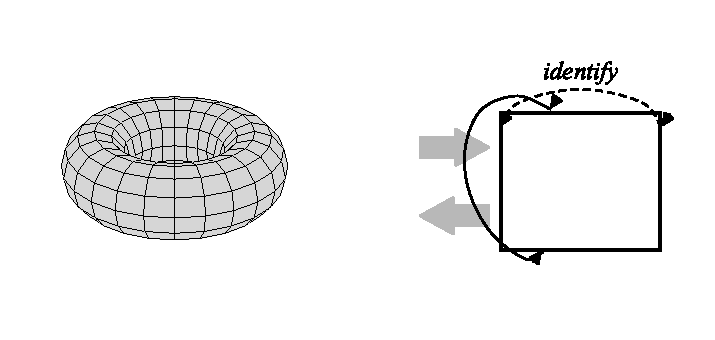
\includegraphics[width=0.72\textwidth]{fig_3.7.pdf}
\caption*{图 3.7\quad 把环面看作平直空间中一个对边被等同起来的正方形。}
\end{figure}
同样，没有什么能阻止我们引入另一个度规使环面不平直；但我们要强调的要点是，它在某个度规之下可以被弄平。每当我们把一个流形嵌入更大的空间，该流形都会从它所嵌入的背景那里继承一个“诱导度规”（induced metric），如附录 A 中所讨论的。我们在这里的要点是：嵌在平直三维欧几里得空间中的环面将具有弯曲的诱导度规，但我们仍然可以选择给它放置另一个不同的度规，使内蕴几何是平直的。

让我们转向一个曲率并不为零的简单例子。我们已经谈论过二维球面 $S^2$，其度规为
\begin{equation*}
ds^2 = a^2(\mathrm{d}\theta^2 + \sin^2\theta\,\mathrm{d}\phi^2),
\tag{3.153}
\end{equation*}
其中 $a$ 是球的半径。如果我们的球嵌在 $\mathbf{R}^3$ 中，它实际上就是半径；但即使没有任何嵌入，我们仍然可以称它为半径。生活在球面上的二维居民想要算出 $a$，可以测量球的面积，除以 $4\pi$，再取平方根；用“半径”一词来指称这个量仅仅是为了方便。我们还应当指出，球的概念有时在更弱的拓扑意义下使用，不假定任何具体的度规；我们使用的这个度规称为\emph{圆度规}（round metric）。不必细究细节，式 (3.153) 的非零联络系数为
\begin{align*}
\Gamma^\theta_{\phi\phi} &= -\sin\theta\cos\theta\\
\Gamma^\phi_{\theta\phi} = \Gamma^\phi_{\phi\theta} &= \cot\theta.
\tag{3.154}
\end{align*}
我们来计算一个颇有希望的 Riemann 张量分量：
\begin{align*}
R^\theta{}_{\phi\theta\phi} &= \partial_\theta\Gamma^\theta_{\phi\phi} - \partial_\phi\Gamma^\theta_{\theta\phi} + \Gamma^\theta_{\theta\lambda}\Gamma^\lambda_{\phi\phi} - \Gamma^\theta_{\phi\lambda}\Gamma^\lambda_{\theta\phi}\\
&= (\sin^2\theta - \cos^2\theta) - (0) + (0) - (-\sin\theta\cos\theta)(\cot\theta)\\
&= \sin^2\theta.
\tag{3.155}
\end{align*}
% ---- 书页 133 / p148 ----
这个记号显然不完美，因为希腊字母 $\lambda$ 是一个被求和的哑指标，而希腊字母 $\theta$ 和 $\phi$ 则代表具体的坐标。下降一个指标，我们得到
\begin{align*}
R_{\theta\phi\theta\phi} &= g_{\theta\lambda}R^\lambda{}_{\phi\theta\phi}\\
&= g_{\theta\theta}R^\theta{}_{\phi\theta\phi}\\
&= a^2\sin^2\theta.
\tag{3.156}
\end{align*}
容易验证，Riemann 张量的所有分量要么为零，要么通过对称性与这个分量相联系。我们可以继续计算 Ricci 张量，利用 $R_{\mu\nu} = g^{\alpha\beta}R_{\alpha\mu\beta\nu}$。我们得到
\begin{align*}
R_{\theta\theta} &= g^{\phi\phi}R_{\phi\theta\phi\theta} = 1\\
R_{\theta\phi} &= R_{\phi\theta} = 0\\
R_{\phi\phi} &= g^{\theta\theta}R_{\theta\phi\theta\phi} = \sin^2\theta.
\tag{3.157}
\end{align*}
Ricci 标量曲率同样直截了当：
\begin{equation*}
R = g^{\theta\theta}R_{\theta\theta} + g^{\phi\phi}R_{\phi\phi} = \frac{2}{a^2}.
\tag{3.158}
\end{equation*}

因此，对二维流形完全刻画了曲率的 Ricci 标量曲率，在整个二维球面上是一个常数。如果我们扰动了这个度规（物理上对应球面上的凹凸不平），情形就不再如此。注意，标量曲率随球半径的增大而减小。即使在更一般的语境中，我们有时也会提到流形的“曲率半径”（radius of curvature），用它来提供一个曲率变化的长度尺度；曲率半径越大，曲率本身越小。

\section{对称性与 Killing 矢量}

真实世界是个乱糟糟的地方，我们别指望找到一个度规，能以完美的精度描述我们实际的宇宙，乃至其任何一个小的部分。我们只能转而借助各种适合于所研究物理情形的近似来为时空建模。例如，恒星或行星外部的几何，可以近似到某种精度地看作球对称的，即使真实情形包含对这种对称性的小偏离——这些偏离可以在以后作为微扰加进来。

广义相对论在这一点上同其他物理学领域并无不同，也对具有对称性的解特别感兴趣。事实上，这类性质在广义相对论中甚至可能比在比如电磁学中更加关键，因为 Einstein 方程（下一章讨论）的非线性本质使得寻找任何精确解都很困难。然而，在弯曲时空的语境下，对于“对称性”究竟意味着什么，我们需要比平时更加小心。本节将发展一些研究对称性的有用工具；更深入的探讨可以在附录 B 中找到。
% ---- 书页 134 / p149 ----
如果几何在一个把 $M$ 映到其自身的变换下不变，我们就认为流形 $M$ 具有一种对称性；也就是说，度规在某种意义上从一点到另一点都是相同的。事实上，不同的张量场可以拥有不同的对称性；度规的对称性称为\textbf{等距变换}（isometries）。有时等距变换的存在是显而易见的；例如考虑四维 Minkowski 空间，
\begin{equation*}
ds^2 = \eta_{\mu\nu}\mathrm{d}x^\mu\mathrm{d}x^\nu = -\mathrm{d}t^2 + \mathrm{d}x^2 + \mathrm{d}y^2 + \mathrm{d}z^2.
\tag{3.159}
\end{equation*}
我们知道这个空间有若干等距变换；它们包括平移（$x^\mu \to x^\mu + a^\mu$，其中 $a^\mu$ 固定）和洛伦兹变换（$x^\mu \to \Lambda^\mu{}_\nu x^\nu$，其中 $\Lambda^\mu{}_\nu$ 是一个洛伦兹变换矩阵）。度规在平移下不变这一点，由一个简单的事实即可立即看出：度规系数 $\eta_{\mu\nu}$ 不依赖于各个坐标函数 $x^\mu$。事实上，只要对某个固定的 $\sigma_*$（但对所有的 $\mu$ 和 $\nu$）都有 $\partial_{\sigma_*}g_{\mu\nu}=0$，就会存在沿 $x^{\sigma_*}$ 方向平移的对称性：
\begin{equation*}
\partial_{\sigma_*}g_{\mu\nu} = 0 \;\;\Rightarrow\;\; x^{\sigma_*} \to x^{\sigma_*} + a^{\sigma_*}\ \text{是一个对称性.}
\tag{3.160}
\end{equation*}

细心的读者会注意到，我们还没有精确定义我们所说的对称性是什么；粗略地说，我们设想度规在某个变换下不变，但精确的含义要到附录 B 中才展开。另外，式 (3.160) 中的蕴含箭头只是单向的，若能有一个干净的判据来判定一个给定的变换何时算作对称性，那就更好了；这一点很快就会讲到。

式 (3.160) 这种形式的等距变换，对测地线方程所描述的检验粒子的运动有直接的推论。回忆式 (3.61)，测地线方程可以用四维动量 $p^\mu = mU^\mu$（至少对类时路径有效）写成
\begin{equation*}
p^\lambda\nabla_\lambda p^\mu = 0.
\tag{3.161}
\end{equation*}
由度规相容性，我们可以自由地下降指标 $\mu$，然后把协变导数展开，得到
\begin{equation*}
p^\lambda\partial_\lambda p_\mu - \Gamma^\sigma_{\lambda\mu}p^\lambda p_\sigma = 0.
\tag{3.162}
\end{equation*}
第一项告诉我们动量的分量沿路径如何变化，
\begin{equation*}
p^\lambda\partial_\lambda p_\mu = m\frac{dx^\lambda}{d\tau}\partial_\lambda p_\mu = m\frac{dp_\mu}{d\tau},
\tag{3.163}
\end{equation*}
% ---- 书页 135 / p150 ----
而第二项则是
\begin{align*}
\Gamma^\sigma_{\lambda\mu}p^\lambda p_\sigma &= \frac{1}{2}g^{\sigma\nu}(\partial_\lambda g_{\mu\nu} + \partial_\mu g_{\nu\lambda} - \partial_\nu g_{\lambda\mu})p^\lambda p_\sigma \tag{3.164}\\
&= \frac{1}{2}(\partial_\lambda g_{\mu\nu} + \partial_\mu g_{\nu\lambda} - \partial_\nu g_{\lambda\mu})p^\lambda p^\nu \tag{3.165}\\
&= \frac{1}{2}(\partial_\mu g_{\nu\lambda})p^\lambda p^\nu,
\tag{3.166}
\end{align*}
其中我们利用了 $p^\lambda p^\nu$ 的对称性从第二行过渡到第三行。于是，在尚未对对称性作任何假设的情况下，我们就看到测地线方程可以写成
\begin{equation*}
m\frac{dp^\mu}{d\tau} = \frac{1}{2}(\partial_\mu g_{\nu\lambda})p^\lambda p^\nu.
\tag{3.167}
\end{equation*}
因此，如果所有的度规系数都不依赖于坐标 $x^{\sigma_*}$，我们就发现这个等距变换蕴含动量分量 $p_{\sigma_*}$ 是该运动的一个守恒量：
\begin{equation*}
\partial_{\sigma_*}g_{\mu\nu} = 0 \;\;\Rightarrow\;\; \frac{dp_{\sigma_*}}{d\tau} = 0.
\tag{3.168}
\end{equation*}

这个结果沿任何测地线都成立，尽管我们只是对类时测地线导出了它。等距变换所蕴含的守恒量，对研究弯曲背景中检验粒子的运动极为有用。

当然，虽然度规分量对一个或多个坐标的独立性蕴含等距变换的存在，反过来却未必成立。例如，洛伦兹变换下的对称性并不表现为 $\eta_{\mu\nu}$ 对任何坐标的独立性；事实上，在四维中共有四类平移和六类洛伦兹变换，总计十个，这显然大于度规可能与之无关的坐标数目。更何况，我们完全可以变换到一个复杂的坐标系，在其中连平移对称性都看不出来。这样的坐标变换会改变度规的分量，却不改变底层的几何——而对称性真正刻画的正是后者。显然，我们需要一个更系统的程序。

我们可以发展出这样一个程序：把式 (3.168) 右边的方程——它表达动量的某个分量为常数——改写成一种协变性更加明显的形式。如果 $x^{\sigma_*}$ 就是 $g_{\mu\nu}$ 与之无关的那个坐标，让我们考虑矢量 $\partial_{\sigma_*}$，把它记作 $K$：
\begin{equation*}
K = \partial_{\sigma_*},
\tag{3.169}
\end{equation*}
用分量记号来写，它等价于
\begin{equation*}
K^\mu = (\partial_{\sigma_*})^\mu = \delta^\mu_{\sigma_*}.
\tag{3.170}
\end{equation*}
我们说矢量 $K^\mu$ 生成（generate）这个等距变换；这意味着，几何在其下不变的变换无穷小地表达为沿 $K^\mu$ 方向的一个移动。
% ---- 书页 136 / p151 ----
同样，这个概念在附录 B 中有更充分的展开。用这个矢量来表示，看上去不具协变形式的量 $p_{\sigma_*}$ 就简单地是
\begin{equation*}
p_{\sigma_*} = K^\nu p_\nu = K_\nu p^\nu.
\tag{3.171}
\end{equation*}
另一方面，这个（标量）量沿路径的恒定性，等价于说它沿测地线的方向导数为零：
\begin{equation*}
\frac{dp_{\sigma_*}}{d\tau} = 0 \;\;\Longleftrightarrow\;\; p^\mu\nabla_\mu(K_\nu p^\nu) = 0.
\tag{3.172}
\end{equation*}
把右边的表达式展开，我们得到
\begin{align*}
p^\mu\nabla_\mu(K_\nu p^\nu) &= p^\mu K_\nu\nabla_\mu p^\nu + p^\mu p^\nu\nabla_\mu K_\nu\\
&= p^\mu p^\nu\nabla_\mu K_\nu\\
&= p^\mu p^\nu\nabla_{(\mu}K_{\nu)},
\tag{3.173}
\end{align*}
其中在第二行我们引用了测地线方程（$p^\mu\nabla_\mu p^\nu = 0$）。在第三行我们利用了 $p^\mu p^\nu$ 在 $\mu$ 和 $\nu$ 上自动对称这一事实，因此只有 $\nabla_\mu K_\nu$ 的对称部分才可能给出贡献。于是我们得出结论：任何满足 $\nabla_{(\mu}K_{\nu)} = 0$ 的矢量 $K_\mu$ 都蕴含 $K_\nu p^\nu$ 沿测地线轨道守恒：
\begin{equation*}
\nabla_{(\mu}K_{\nu)} = 0 \;\;\Rightarrow\;\; p^\mu\nabla_\mu(K_\nu p^\nu) = 0.
\tag{3.174}
\end{equation*}

左边的方程称为\textbf{Killing 方程}（Killing's equation），满足它的矢量场称为\textbf{Killing 矢量场}（Killing vector fields，或简称 Killing 矢量）。你可以自己验证：如果度规不依赖于某个坐标 $x^{\sigma_*}$，矢量 $\partial_{\sigma_*}$ 将满足 Killing 方程。事实上，如果一个矢量 $K^\mu$ 满足 Killing 方程，那么总能找到一个坐标系使得 $K = \partial_{\sigma_*}$；但一般说来，我们无法找到一个坐标系使所有 Killing 矢量都同时取这种形式，而且矢量要满足 Killing 方程也并不需要这种形式。

正如我们将在附录 B 中研究的，流形上的 Killing 矢量场与该流形上度规的连续对称性一一对应。每个 Killing 矢量都蕴含着与测地线运动相联系的守恒量的存在。这一点可以从物理上理解：按定义，度规沿 Killing 矢量的方向是不变的。粗略地说，自由粒子在这个方向上不会感到任何力，因而其动量在这个方向上的分量将相应地守恒。事实上，我们用来证明“若 $\nabla_{(\mu}K_{\nu)} = 0$ 则 $K_\nu p^\nu$ 沿测地线守恒”的那类逻辑，可以推广到更多的指标：\textbf{Killing 张量}（Killing tensor）是一个对称的 $\ell$ 指标张量 $K_{\nu_1\ldots\nu_\ell}$，它满足 Killing 方程的显而易见的推广，并相应地通过与 $\ell$ 份动量缩并而导致守恒量：
% ---- 书页 137 / p152 ----
\begin{equation*}
\nabla_{(\mu}K_{\nu_1\ldots\nu_\ell)} = 0 \;\;\Rightarrow\;\; p^\mu\nabla_\mu(K_{\nu_1\ldots\nu_\ell}p^{\nu_1}\cdots p^{\nu_\ell}) = 0.
\tag{3.175}
\end{equation*}

Killing 张量的简单例子有度规本身，以及 Killing 矢量的对称化张量积。Killing 张量与时空中对称性的联系并不简单，但它们将简化我们对转动黑洞和膨胀宇宙的分析。

Killing 矢量的导数可以通过下式与 Riemann 张量联系起来
\begin{equation*}
\nabla_\mu\nabla_\sigma K^\rho = R^\rho{}_{\sigma\mu\nu}K^\nu,
\tag{3.176}
\end{equation*}
正如习题中要求你们证明的那样。把这个表达式缩并，得到
\begin{equation*}
\nabla_\mu\nabla_\sigma K^\mu = R_{\sigma\nu}K^\nu.
\tag{3.177}
\end{equation*}
这些关系连同 Bianchi 恒等式与 Killing 方程，足以证明 Ricci 标量曲率沿 Killing 矢量场的方向导数为零，
\begin{equation*}
K^\lambda\nabla_\lambda R = 0.
\tag{3.178}
\end{equation*}

最后这个事实从另一个侧面反映了这样的观念：几何沿 Killing 矢量场不发生变化。

除了为单个粒子的运动导致守恒量之外，类时 Killing 矢量的存在还使我们能够为整个时空定义一个守恒的能量。给定一个 Killing 矢量 $K_\nu$ 和一个守恒的能量-动量张量 $T_{\mu\nu}$，我们可以构造一个流
\begin{equation*}
J^\mu_T = K_\nu T^{\mu\nu}
\tag{3.179}
\end{equation*}
它自动守恒，
\begin{align*}
\nabla_\mu J^\mu_T &= (\nabla_\mu K_\nu)T^{\mu\nu} + K_\nu(\nabla_\mu T^{\mu\nu})\\
&= 0.
\tag{3.180}
\end{align*}
第一项由于 Killing 方程而为零（因为上指标的对称性恰好使下指标自动对称化），第二项则由于 $T_{\mu\nu}$ 的守恒而为零。如果 $K_\nu$ 是类时的，我们可以在一个类空超曲面 $\Sigma$ 上积分来定义总能量，
\begin{equation*}
E_T = \int_\Sigma J^\mu_T n_\mu \sqrt{\gamma}\,\mathrm{d}^3x,
\tag{3.181}
\end{equation*}
其中 $\gamma_{ij}$ 是 $\Sigma$ 上的诱导度规，$n_\mu$ 是 $\Sigma$ 的法矢量。在附录 E 中我们将讨论超曲面上的积分，特别是 Stokes 定理；正如那里所解释的，$E_T$ 在任何类空超曲面上积分都得到相同的值，因而是守恒的。
% ---- 书页 138 / p153 ----
这个结果与我们在第 3.5 节中的讨论相当契合：在那里我们发现，在一个膨胀的宇宙中总能量通常不守恒；膨胀意味着度规随时间变化，因此在这个方向上没有等距变换。当存在类时 Killing 矢量时，我们可以把度规写成不依赖于类时坐标的形式，而诺特定理便蕴含一个守恒的能量。类似地，类空 Killing 矢量可以用来构造守恒的动量（或角动量）。

虽然在任意给定的时空中实际求解 Killing 方程可能简单也可能不简单，但通过直接观察写下某些 Killing 矢量往往是可能的。（当然，一个一般的度规可能根本没有任何 Killing 矢量，但为了保持简单，我们经常处理具有高度对称性的度规。）例如，在具有度规 $\mathrm{d}s^2 = \mathrm{d}x^2 + \mathrm{d}y^2 + \mathrm{d}z^2$ 的 $\mathbf{R}^3$ 中，度规分量对 $x$、$y$、$z$ 的无关性立即给出三个 Killing 矢量：
\begin{align*}
X^\mu &= (1,\, 0,\, 0)\\
Y^\mu &= (0,\, 1,\, 0)\\
Z^\mu &= (0,\, 0,\, 1).
\tag{3.182}
\end{align*}
这些显然代表三个平移。$\mathbf{R}^3$ 中还有三个转动对称性，它们就不那么简单了。为了找到它们，设想先变换到球坐标，
\begin{align*}
x &= r\sin\theta\cos\phi\\
y &= r\sin\theta\sin\phi\\
z &= r\cos\theta,
\tag{3.183}
\end{align*}
此时度规取如下形式
\begin{equation*}
ds^2 = \mathrm{d}r^2 + r^2\mathrm{d}\theta^2 + r^2\sin^2\theta\,\mathrm{d}\phi^2.
\tag{3.184}
\end{equation*}
现在这个度规（还是\emph{同一个}度规，只是换了一个坐标系）明显不依赖于 $\phi$。因此我们知道 $R = \partial_\phi$ 是一个 Killing 矢量。变换回笛卡尔坐标，它就成为
\begin{equation*}
R = -y\partial_x + x\partial_y.
\tag{3.185}
\end{equation*}
于是 $R^\mu$ 的笛卡尔分量就是 $(-y,\, x,\, 0)$。由于这代表绕 $z$ 轴的一个转动，不难猜出所有三个转动 Killing 矢量的分量：
\begin{align*}
R^\mu &= (-y,\; x,\; 0)\\
S^\mu &= (\phantom{-}z,\; 0,\; -x)\\
T^\mu &= (\;0,\; -z,\; y),
\tag{3.186}
\end{align*}
% ---- 书页 139 / p154 ----
分别代表绕 $z$、$y$、$x$ 轴的转动。你可以自己验证，这些矢量确实求解 Killing 方程。整体的正负号无关紧要，因为一个 Killing 矢量加负号仍然是 Killing 矢量。

这个练习直接引出二维球面 $S^2$ 的 Killing 矢量，其度规为
\begin{equation*}
ds^2 = \mathrm{d}\theta^2 + \sin^2\theta\,\mathrm{d}\phi^2.
\tag{3.187}
\end{equation*}
由于这个球可以看作 $\mathbf{R}^3$ 中到原点距离为 1 的点的轨迹，而各个转动的 Killing 矢量都把这样一个球转成它自身，所以它们也表示 $S^2$ 的对称性。为了得到这些矢量的明显的坐标基表示，我们先把三维矢量 (3.186) 变换到球坐标 $x^{\mu'} = (r, \theta, \phi)$。一番直截了当的计算给出
\begin{align*}
R &= \partial_\phi\\
S &= \cos\phi\,\partial_\theta - \cot\theta\sin\phi\,\partial_\phi\\
T &= -\sin\phi\,\partial_\theta - \cot\theta\cos\phi\,\partial_\phi.
\tag{3.188}
\end{align*}
注意，这里没有沿 $\partial_r$ 的分量，这对一个转动的等距变换来说正合情理。因此，$\mathbf{R}^3$ 中三个转动 Killing 矢量的表达式 (3.188)，与球坐标下 $S^2$ 的那些表达式完全相同。

在 $n\geq 2$ 维时，Killing 矢量的数目可以多于维数。这是因为一组 Killing 矢量场可以线性无关，尽管在流形上任何一点处，该点上的这些矢量是线性相关的。证明 Killing 矢量以\emph{常数}系数的线性组合仍是 Killing 矢量是很容易的（所以你应该自己动手做一下；此时该线性组合不再算作一个独立的 Killing 矢量），但对于在流形上变化的系数，这一般不再成立。你还可以证明，两个 Killing 矢量场的对易子是一个 Killing 矢量场；知道这一点非常有用，但对易子给出的矢量场可能不是线性无关的（也可能干脆为零）。因此，求出一个度规的所有 Killing 矢量这个问题颇为棘手，因为什么时候该停止寻找并不总是清楚的。

\section{最大对称空间}

一个空间究竟能有多对称？具有最高可能对称度的空间的一个例子，是带有平直欧几里得度规的 $\mathbf{R}^n$。让我们从它们在某个固定点 $p$ 的邻域内做什么这个角度，来考察这个空间的等距变换——我们知道它们就是 $n$ 维中的平移和转动。平移是移动该点的那些变换；可以有 $n$ 个独立的轴沿着移动它，所以平移总共 $n$ 个。以 $p$ 为中心的转动是使 $p$ 保持不变的那些变换；可以把它们看作把过 $p$ 的一根轴转到另一根轴。轴共有 $n$ 根，每根轴可以转到另外 $n-1$ 根上去，但我们不应把“$y$ 转到 $x$”同“$x$ 转到 $y$”算作不同的转动，所以独立转动的总数是 $\frac{1}{2}n(n-1)$。于是我们有
\begin{equation*}
n + \frac{1}{2}n(n-1) = \frac{1}{2}n(n+1)
\tag{3.189}
\end{equation*}
个 $\mathbf{R}^n$ 的独立对称性。但我们的计数论证只涉及对称性在 $p$ 的邻域内的行为，而不是全局地遍及整个流形；所以即使存在曲率，这个计数也应相同。如果度规号差不是欧几里得型的，某些转动实际上会是推动（boost），但同样计数不变。等距变换的数目当然就是线性无关的 Killing 矢量场的数目。因此，我们把具有 $\frac{1}{2}n(n+1)$ 个 Killing 矢量的 $n$ 维流形称为\textbf{最大对称空间}（maximally symmetric space）。最大对称空间最熟悉的例子是 $n$ 维欧几里得空间 $\mathbf{R}^n$ 和 $n$ 维球面 $S^n$。对 $n$ 维球面，我们通常把等距变换看作由 $\frac{1}{2}n(n+1)$ 个独立转动组成，而不是转动和平移的某种混合集合。然而，如果考虑这些转动作用在某个固定点 $p$ 上，稍想片刻就会使我们确信：整个集合可以分解为绕该点的 $\frac{1}{2}n(n-1)$ 个转动（保持 $p$ 不动），以及另外 $n$ 个沿各个方向移动 $p$ 的转动，正如在 $\mathbf{R}^n$ 中那样。
% ---- 书页 140 / p155 ----
如果一个流形是最大对称的，那么曲率处处相同（正如平移类的等距变换所表达的那样），并且沿每个方向都相同（正如转动类的等距变换所表达的那样）。因此，只要知道了最大对称空间在一点的曲率，我们就知道了它所有的曲率。事实上，可能的最大对称空间只有寥寥数种；对它们进行分类的，是标量曲率 $R$（它将处处为常数）、维数 $n$、度规号差，或许还有与整体拓扑有关的一些分立信息（例如把 $n$ 维环面同 $\mathbf{R}^n$ 区分开来，以及把大小不同的环面彼此区分开）。由此可知，我们应当能够由 Ricci 标量 $R$ 重建这类空间的整个 Riemann 张量；让我们看看这是如何做到的。

基本想法很简单：既然几何在所有方向上看起来都一样，曲率张量在所有方向上也应该看起来一样。这可能意味着什么呢？先在某点 $p$ 选取局部惯性坐标，使得 $g_{\hat\mu\hat\nu} = \eta_{\hat\mu\hat\nu}$。当然，局部惯性坐标并不唯一；例如，我们可以在 $p$ 点作一个洛伦兹变换，度规分量仍将保持为 $\eta_{\hat\mu\hat\nu}$。（所谓“作一个洛伦兹变换”，我们实际上指的是改变 $T_p$ 中的基矢；在弯曲时空中，这只在单个点上有意义，而不是在一个区域上。）既然几何是最大对称的，我们希望 Riemann 张量也是如此；也就是说，$R_{\hat\rho\hat\sigma\hat\mu\hat\nu}$ 的分量在洛伦兹变换下也不应改变，因为时空中没有任何从优的方向。但在洛伦兹变换下分量不变的张量是独一无二的几种——度规、Kronecker $\delta$，以及 Levi-Civita 张量。
% ---- 书页 141 / p156 ----
这意味着，在这些坐标下、在这个点上，$R_{\hat\rho\hat\sigma\hat\mu\hat\nu}$ 的分量将正比于一个由这些不变张量构造出来的张量。尝试匹配 Riemann 张量的对称性就会发现，唯一的可能是
\begin{equation*}
R_{\hat\rho\hat\sigma\hat\mu\hat\nu} \propto g_{\hat\rho\hat\mu}g_{\hat\sigma\hat\nu} - g_{\hat\rho\hat\nu}g_{\hat\sigma\hat\mu}.
\tag{3.190}
\end{equation*}

但这是一个完全张量性的关系，所以它在任何坐标系中都必须成立。我们是在单个点 $p$ 处论证这个关系的，但在最大对称空间中所有的点生而平等，所以它在任何其他点上也必定成立。比例常数很容易固定：把两边缩并两次［左边变成 $R$，右边为 $n(n-1)$］。我们最终得到一个在任何最大对称空间中、在任何点、在任何坐标系里都成立的方程：
\begin{equation*}
R_{\rho\sigma\mu\nu} = \frac{R}{n(n-1)}(g_{\rho\mu}g_{\sigma\nu} - g_{\rho\nu}g_{\sigma\mu}).
\tag{3.191}
\end{equation*}

同样地，如果 Riemann 张量满足这个条件（其中 $R$ 在流形上为常数），那么度规就是最大对称的。在二维中，发现 $R$ 是常数就足以证明空间是最大对称的，因为曲率只有一个独立分量。在更高维时你就得多费些力气了。

于是，在局域上（暂且不管整体拓扑的问题），给定维数和号差的最大对称空间完全由 $R$ 确定。这类空间的基本分类，就是看 $R$ 为正、为零还是为负，因为 $R$ 的大小代表着空间尺寸的整体标度。对欧几里得号差，平直的最大对称空间是平面或适当的高维推广，而正曲率的则是球面。负曲率的最大对称欧几里得空间是双曲面（hyperboloid），记作 $H^n$。这些空间比较不为人熟悉，因为即使是二维双曲面也无法等距地嵌入 $\mathbf{R}^3$。让我们简要考察一下这个二维双曲面。

表示 $H^2$（它与 $\mathbf{R}^2$ 有相同的拓扑）的方式有好几种。一种简单的方式是把它们表示为\textbf{庞加莱半平面}（Poincaré half-plane），它是带有坐标 $\{x, y\}$ 的二维区域中 $y > 0$ 的部分，其度规为
\begin{equation*}
ds^2 = \frac{a^2}{y^2}(\mathrm{d}x^2 + \mathrm{d}y^2).
\tag{3.192}
\end{equation*}

庞加莱半平面的几何当然不同于 $\mathbf{R}^2$ 上半部分的几何，尽管使用了相似的坐标。例如，我们可以计算一条从 $y_1$ 竖直地（$x$ 为常数）延伸到 $y_2$ 的线段的长度：
% ---- 书页 142 / p157 ----
\begin{align*}
\Delta s &= \int_{y_1}^{y_2}\sqrt{g_{\mu\nu}\frac{\mathrm{d}x^\mu}{\mathrm{d}y}\frac{\mathrm{d}x^\nu}{\mathrm{d}y}}\,\mathrm{d}y\\
&= a\int_{y_1}^{y_2}\frac{\mathrm{d}y}{y}\\
&= a\ln\left(\frac{y_2}{y_1}\right).
\tag{3.193}
\end{align*}

这根本不是我们在欧几里得空间中所预期的结果 $\Delta s = y_2 - y_1$。特别地，注意对于趋近边界 $y = 0$ 的路径，路径长度变为无穷。换句话说，它其实根本算不上什么边界；就生活在双曲面上的任何居民而言，它无限遥远。

式 (3.192) 的非零 Christoffel 符号为
\begin{align*}
\Gamma^x_{xy} &= \Gamma^x_{yx} = -y^{-1}\\
\Gamma^y_{xx} &= y^{-1}\\
\Gamma^y_{yy} &= -y^{-1}.
\tag{3.194}
\end{align*}
由此出发容易证明，测地线满足
\begin{equation*}
(x - x_0)^2 + y^2 = l^2,
\tag{3.195}
\end{equation*}
其中 $x_0$ 和 $l$ 为常数。这种形式的曲线是圆心位于 $x$ 轴上的半圆，如图 3.8 所示。在 $x_0 \to \infty$、$l \to \infty$ 而 $l - x_0$ 固定的极限下，我们得到一条竖直的直线。仿照我们在第 3.7 节末尾对 $S^2$ 的讨论，我们算得 Riemann 张量的一个代表性分量为
\begin{equation*}
R^x{}_{yxy} = -y^{-2}.
\tag{3.196}
\end{equation*}

\begin{figure}[H]
\centering
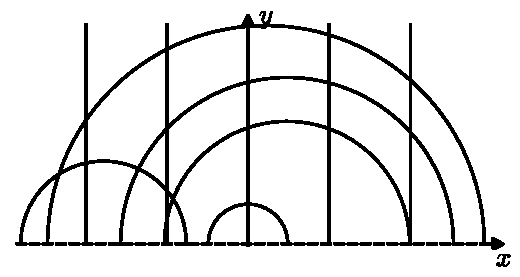
\includegraphics[width=0.72\textwidth]{fig_3.8.pdf}
\caption*{图 3.8\quad 带负曲率度规的上半平面。测地线是与 $x$ 轴垂直相交的半圆和直线。}
\end{figure}
与二维球面一样，所有其他分量要么为零，要么通过对称性与该分量相联系。这不过是反映了这样一个事实：我们正处在二维
% 本块末句在原书书页143顶部继续（"mensions, ..."），下一块请用 %JOIN% 续接本句。
 ，曲率只有一个独立分量。如法炮制，便得到 Ricci 张量
% ---- 书页 143 / p158 ----
\begin{gather*}
R_{xx} = -y^{-2}\\
R_{xy} = 0\\
R_{yy} = -y^{-2},
\tag{3.197}
\end{gather*}

以及标量曲率，
\begin{equation*}
R = -\frac{2}{a^{2}}.
\tag{3.198}
\end{equation*}

我们看到，它与 $S^{2}$ 的情形符号相反，而且特别值得注意的是，它是一个常数。由于我们处在二维，这就足以保证我们的度规确实是最大对称的。当然，还存在另一些坐标，$H^{2}$ 在其中看起来十分不同；习题中会引入其中一种。

于是，在局域上，欧几里得号差的最大对称空间依 $R$ 的符号而为平面、球面或双曲面三者之一。在整体上，任何（欧几里得号差的）最大对称空间都可以这样构造出来：从这三种空间之一中仔细选取一个区域，并把不同的边两两认同，正如平直环面可以由 $\mathbf{R}^{2}$ 构造那样。顺带提一句，让我们简短地谈一谈局域几何与整体拓扑之间的一种联系，它被囊括在 Gauss–Bonnet 定理之中。对于二维紧致无边、可定向的流形，这个定理说
\begin{equation*}
\chi(M) = \frac{1}{4\pi}\int_{M} R\sqrt{|g|}\,\mathrm{d}^{n}x,
\tag{3.199}
\end{equation*}
（译注：原书印作 $\mathrm{d}^{n}x$；就二维曲面而言，按上下文应为 $\mathrm{d}^{2}x$。）

其中 $\chi(M)$ 是该空间的一个拓扑不变量，称为 Euler 示性数（Euler characteristic）。一般说来，它可以由第 2 章提到过的那些上同调空间计算出来；不过在二维情形，它就简单地由下式给出
\begin{equation*}
\chi(M) = 2(1 - g),
\tag{3.200}
\end{equation*}

其中 $g$ 是曲面的亏格（对球面为零，对环面或黎曼面则等于柄的数目）。无论曲率 $R$ 是不是常数，Gauss–Bonnet 定理都成立；然而当 $R$ 是常数时，我们看到所有亏格 $g \geq 2$ 的黎曼面必定具有负曲率，正如球面必定正弯曲、而环面必定平直一样。

继续我们的题外话，暂且来想一想弦论（string theory），它宣称构成宇宙的基本对象是细小的一维弦圈。这样的弦具有二维的“世界面”（world-sheet），而不是一维的世界线。在弦论中做微扰论（相当于量子场论中计算 Feynman 图）涉及对所有世界面几何求和（出于技术上的原因，一般取欧几里得几何）。这听起来像是数目庞大的一堆几何，但在二维中，任何度规都可以写成某个基准度规（fiducial metric）乘以一个共形因子（conformal factor）。这是可信的，因为曲率只有一个分量；习题会请你证明这一点。基准度规可以对每一种世界面拓扑分别选取，而我们不妨把它选成（局域上的）最大对称度规，好让日子好过一些——亏格零用标准的圆球面，亏格一用平面，更高的亏格用双曲面。更加幸运的是，物理上最令人感兴趣的弦论是所谓的临界弦论（critical string theories），对于它们，共形因子本身根本无关紧要。这正是使微扰弦论中的计算成为可能的原因之一；我们只需对一个离散的拓扑集合求和，而且每种拓扑只有有限多个模参数（modular parameters），比如那些告诉我们环面各方向尺寸的参数。

% ---- 书页 144 / p159 ----
我们用最后一个论点来为本节收尾。我们已经探索了具有欧几里得号差的最大对称空间；当然，也存在具有洛伦兹号差的相应时空。我们知道，$R = 0$ 的最大对称时空正是 Minkowski 空间。正曲率的最大对称时空被称为 de Sitter 空间，而负曲率的那个则被颇具想象力地贴上了反 de Sitter 空间的标签。这些时空将在第 8 章中得到更透彻的讨论。

到现在你们应该已经清楚，各附录以重要的方式充实了这些思想。性急的读者可以跳过它们，但那样做未免可惜。

\section{测地偏离}

Riemann 张量作为曲率的后果而露面的又一种方式是：测地偏离。你们无疑听说过，欧几里得（平直）几何的定义性性质是平行公设（parallel postulate）：起初平行的直线永远保持平行。当然，在弯曲空间里这并不成立；在球面上，起初平行的测地线最终必定相交。我们想在任意弯曲空间中把这种行为定量地刻画出来。

问题在于，“平行”这个概念并不能自然地从平直空间延伸到弯曲空间。我们所能做到的最好的事情，是考虑那些可能起初平行的测地线曲线，看看当我们沿着测地线走下去时它们表现如何。为此，我们考虑一个单参数测地线族 $\gamma_{s}(t)$。也就是说，对每个 $s\in\mathbf{R}$，$\gamma_{s}$ 是一条以仿射参量 $t$ 参数化的测地线。这些曲线的集合定义了一张光滑的二维曲面（嵌入在任意维数的流形 $M$ 中）。只要所选的这族测地线互不相交，曲面上的坐标就可以取为 $s$ 和 $t$。整张曲面就是点集 $x^{\mu}(s,t)\in M$。我们有两个自然的矢量场：测地线的切矢量，
\begin{equation*}
T^{\mu} = \frac{\partial x^{\mu}}{\partial t},
\tag{3.201}
\end{equation*}

% ---- 书页 145 / p160 ----
\begin{figure}[H]
\centering
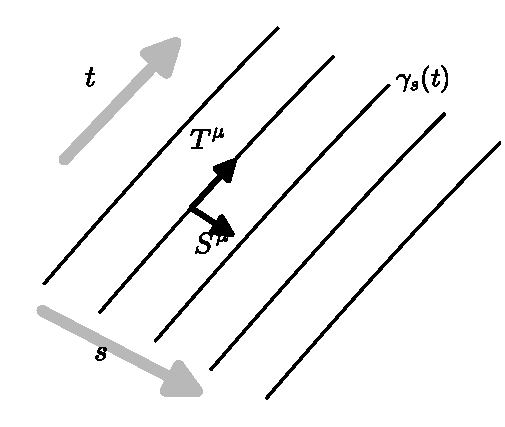
\includegraphics[width=0.72\textwidth]{fig_3.9.pdf}
\caption*{图 3.9\quad 一族测地线 $\gamma_{s}(t)$，及其切矢量 $T^{\mu}$。矢量场 $S^{\mu}$ 量度邻近测地线之间的偏离。}
\end{figure}

以及偏离矢量（deviation vectors）
\begin{equation*}
S^{\mu} = \frac{\partial x^{\mu}}{\partial s}.
\tag{3.202}
\end{equation*}

这个名称来自如下非正式的观念：$S^{\mu}$ 从一条测地线指向邻近的那些测地线。

$S^{\mu}$ 从一条测地线指向下一条测地线的想法，启发我们定义“测地线的相对速度”（relative velocity of geodesics），
\begin{equation*}
V^{\mu} = (\nabla_{T}S)^{\mu} = T^{\rho}\nabla_{\rho}S^{\mu},
\tag{3.203}
\end{equation*}

以及“测地线的相对加速度”（relative acceleration of geodesics），
\begin{equation*}
A^{\mu} = (\nabla_{T}V)^{\mu} = T^{\rho}\nabla_{\rho}V^{\mu}.
\tag{3.204}
\end{equation*}

这些名字你们听听就好，不必太较真，但这些矢量无疑是良定义的。测地线之间这种\emph{相对}加速度的概念，应当与一条路径偏离测地线运动的加速度区分开来；后者（当 $t$ 为固有时）由 $a^{\mu} = T^{\sigma}\nabla_{\sigma}T^{\mu}$ 给出。

由于 $S$ 和 $T$ 是适配于某个坐标系的基矢量，它们的对易子为零：
\begin{equation*}
[S, T] = 0.
\tag{3.205}
\end{equation*}

由式 (3.37) 我们于是有
\begin{equation*}
S^{\rho}\nabla_{\rho}T^{\mu} = T^{\rho}\nabla_{\rho}S^{\mu}.
\tag{3.206}
\end{equation*}

% ---- 书页 146 / p161 ----
记住这一点，我们来计算加速度：
\begin{align*}
A^{\mu} &= T^{\rho}\nabla_{\rho}(T^{\sigma}\nabla_{\sigma}S^{\mu})\\
&= T^{\rho}\nabla_{\rho}(S^{\sigma}\nabla_{\sigma}T^{\mu})\\
&= (T^{\rho}\nabla_{\rho}S^{\sigma})(\nabla_{\sigma}T^{\mu}) + T^{\rho}S^{\sigma}\nabla_{\rho}\nabla_{\sigma}T^{\mu}\\
&= (S^{\rho}\nabla_{\rho}T^{\sigma})(\nabla_{\sigma}T^{\mu}) + T^{\rho}S^{\sigma}(\nabla_{\sigma}\nabla_{\rho}T^{\mu} + R^{\mu}{}_{\nu\rho\sigma}T^{\nu})\\
&= (S^{\rho}\nabla_{\rho}T^{\sigma})(\nabla_{\sigma}T^{\mu}) + S^{\sigma}\nabla_{\sigma}(T^{\rho}\nabla_{\rho}T^{\mu}) - (S^{\sigma}\nabla_{\sigma}T^{\rho})\nabla_{\rho}T^{\mu}\\
&\qquad + R^{\mu}{}_{\nu\rho\sigma}T^{\nu}T^{\rho}S^{\sigma}\\
&= R^{\mu}{}_{\nu\rho\sigma}T^{\nu}T^{\rho}S^{\sigma}.
\tag{3.207}
\end{align*}

让我们逐行琢磨一下。第一行是 $A^{\mu}$ 的定义；第二行直接来自式 (3.206)；第三行不过是 Leibniz 律；第四行用相反次序的导数加上 Riemann 张量，取代了那个双重协变导数；在第五行我们再次使用 Leibniz 律（这一次与通常的次序相反），然后消去两个相同的项，并注意到含 $T^{\rho}\nabla_{\rho}T^{\mu}$ 的项为零，因为 $T^{\mu}$ 是测地线的切矢量。得到的结果，
\begin{equation*}
\boxed{\,A^{\mu} = \frac{D^{2}}{dt^{2}}S^{\mu} = R^{\mu}{}_{\nu\rho\sigma}T^{\nu}T^{\rho}S^{\sigma}\,,}
\tag{3.208}
\end{equation*}

就是\textbf{测地偏离方程}。它表达了一件我们可能早已预料到的事情：两条相邻测地线之间的相对加速度正比于曲率。

测地偏离方程刻画的是一个单参数相邻测地线族的行为。我们有时也会有兴趣追踪一个多维的相邻测地线集合的行为，比如它可能代表一束光子，或者一份有质量检验粒子的分布。这样的测地线集合构成一个线汇（congruence）；在附录 F 中，我们将推导描述这类线汇演化的方程。

当然，从物理上看，相邻测地线的加速度被解释为引力潮汐力的一种表现。在下一章中，我们将更详细地探讨弯曲时空的性质如何反映在引力场中的物理里。

\section{习题}

% 习题编号照原书
\textbf{1.}\quad 验证度规相容性（$\nabla_{\sigma}g_{\mu\nu}=0$）的下列推论：
\begin{gather*}
\nabla_{\sigma}g^{\mu\nu} = 0\\
\nabla_{\lambda}\epsilon_{\mu\nu\rho\sigma} = 0.
\tag{3.209}
\end{gather*}

% ---- 书页 147 / p162 ----
\textbf{2.}\quad 你们已经熟悉三维欧几里得空间中普通矢量分析里的梯度（$\nabla\phi$）、散度（$\nabla\cdot\mathbf{V}$）和旋度（$\nabla\times\mathbf{V}$）这几种运算。请使用协变导数，在由
\begin{equation*}
x = r\sin\theta\cos\phi
\tag{3.210}
\end{equation*}
\begin{equation*}
y = r\sin\theta\sin\phi
\tag{3.211}
\end{equation*}
\begin{equation*}
z = r\cos\theta.
\tag{3.212}
\end{equation*}
所定义的球坐标 $\{r,\theta,\phi\}$ 中，推导这些运算的公式。把你的结果与 Jackson (1999) 或同类的教材相比较。它们完全相同吗？它们应当完全相同吗？

\textbf{3.}\quad 想象我们有一个\emph{对角}的度规 $g_{\mu\nu}$。证明 Christoffel 符号由下式给出：
\begin{equation*}
\Gamma^{\lambda}_{\mu\nu} = 0
\tag{3.213}
\end{equation*}
\begin{equation*}
\Gamma^{\lambda}_{\mu\mu} = -\frac{1}{2}(g_{\lambda\lambda})^{-1}\partial_{\lambda}g_{\mu\mu}
\tag{3.214}
\end{equation*}
\begin{equation*}
\Gamma^{\lambda}_{\mu\lambda} = \partial_{\mu}\left(\ln\sqrt{|g_{\lambda\lambda}|}\right)
\tag{3.215}
\end{equation*}
\begin{equation*}
\Gamma^{\lambda}_{\lambda\lambda} = \partial_{\lambda}\left(\ln\sqrt{|g_{\lambda\lambda}|}\right)
\tag{3.216}
\end{equation*}
在这些式子中，$\mu\neq\nu\neq\lambda$，而且重复指标\emph{不}作求和。

\textbf{4.}\quad 在欧几里得三维空间中，我们可以经由
\begin{equation*}
x = uv\cos\phi\qquad y = uv\sin\phi\qquad z = \frac{1}{2}(u^{2}-v^{2}).
\end{equation*}
定义抛物面坐标（paraboloidal coordinates）$(u,v,\phi)$。

\textbf{(a)}\quad 求抛物面坐标与笛卡尔坐标之间的坐标变换矩阵 $\partial x^{\alpha}/\partial x^{\beta'}$ 以及逆变换。这个映射中存在奇点吗？

\textbf{(b)}\quad 用笛卡尔的基矢量与基 1-形式表出抛物面坐标的基矢量与基 1-形式。

\textbf{(c)}\quad 求抛物面坐标中的度规与逆度规。

\textbf{(d)}\quad 计算 Christoffel 符号。

\textbf{(e)}\quad 计算散度 $\nabla_{\mu}V^{\mu}$ 与拉普拉斯算符（Laplacian）$\nabla_{\mu}\nabla^{\mu}f$。

\textbf{5.}\quad 考虑一个二维球面，坐标为 $(\theta,\phi)$，度规为
\begin{equation*}
\mathrm{d}s^{2} = \mathrm{d}\theta^{2} + \sin^{2}\theta\,\mathrm{d}\phi^{2}.
\tag{3.217}
\end{equation*}

\textbf{(a)}\quad 证明经线（$\phi=$ 常数）都是测地线，并证明纬线（$\theta=$ 常数）中唯一的一条测地线是赤道（$\theta=\pi/2$）。

\textbf{(b)}\quad 取一个分量为 $V^{\mu}=(1,0)$ 的矢量，让它沿一条等纬度的圆周平行移动一整周。所得到的矢量分量作为 $\theta$ 的函数是什么？

\textbf{6.}\quad 地球表面之外的度规的一个良好近似由下式给出：
\begin{equation*}
\mathrm{d}s^{2} = -(1+2\Phi)\mathrm{d}t^{2} + (1-2\Phi)\mathrm{d}r^{2} + r^{2}(\mathrm{d}\theta^{2} + \sin^{2}\theta\,\mathrm{d}\phi^{2}),
\tag{3.218}
\end{equation*}

% ---- 书页 148 / p163 ----
其中
\begin{equation*}
\Phi = -\frac{GM}{r}
\tag{3.219}
\end{equation*}
可以认为是我们所熟悉的 Newton 引力势。这里 $G$ 是 Newton 引力常数，$M$ 是地球的质量。在本题中可以假设 $\Phi$ 为小量。

\textbf{(a)}\quad 想象在地球表面上、距地心 $R_{1}$ 处有一只钟，而在一座高楼上、距地心 $R_{2}$ 处有另一只钟。试计算每只钟上经历的时间作为坐标时 $t$ 的函数。哪只钟走得更快？

\textbf{(b)}\quad 求出与绕地球赤道（$\theta=\pi/2$）的圆轨道相对应的测地线。$\mathrm{d}\phi/\mathrm{d}t$ 等于多少？

\textbf{(c)}\quad 一颗半径为 $R_{1}$ 的卫星（贴着地面掠过，忽略空气阻力）绕行一整周期间，经历多少固有时？你不妨只算到 $\Phi$ 的一阶。代入地球半径等的实际数值（别忘了把光速恢复进去），得到一个以秒作单位的答案。这个数与静止在地球表面的那只钟上经历的固有时相比如何？

\textbf{7.}\quad 本题中你要利用附录 I 中引入的平行移动传播子（parallel propagator），来看看 Riemann 张量如何从绕一个无穷小回路的平行移动中产生。考虑如下回路：

\begin{figure}[H]
\centering
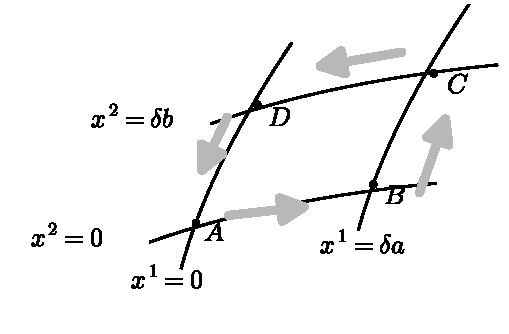
\includegraphics[width=0.72\textwidth]{fig_3.11-ex7.pdf}
\caption*{图 3.11-ex7\quad 习题 7 的无穷小回路：由 $x^{1}=0$ 与 $x^{1}=\delta a$、$x^{2}=0$ 与 $x^{2}=\delta b$ 四条曲线围成，顶点为 $A$、$B$、$C$、$D$，箭头标出沿 $A\to B\to C\to D\to A$ 的平行移动方向。}
\end{figure}

利用平行移动传播子的无穷级数表达式，计算一个矢量沿此回路从 $A$ 到 $B$ 到 $C$ 到 $D$ 再回到 $A$ 平行移动一周所诱导的变换，准确到 $\delta a$ 和 $\delta b$ 的最低非平凡阶，并证明它正比于 Riemann 张量的相应分量。为了让事情容易些，你可以在旅程的适当路段上取 $x^{1}$ 和 $x^{2}$ 作为参量。

\textbf{8.}\quad 三维球面在坐标 $x^{\mu}=(\psi,\theta,\phi)$ 下的度规可以写成
\begin{equation*}
\mathrm{d}s^{2} = \mathrm{d}\psi^{2} + \sin^{2}\psi(\mathrm{d}\theta^{2} + \sin^{2}\theta\,\mathrm{d}\phi^{2}).
\tag{3.220}
\end{equation*}

% ---- 书页 149 / p164 ----
\textbf{(a)}\quad 计算 Christoffel 联络系数。用什么方法都可以，但通过对积分 (3.49) 作变分来得到联络系数是一种很好的练习。

\textbf{(b)}\quad 计算 Riemann 张量、Ricci 张量和 Ricci 标量。

\textbf{(c)}\quad 证明该度规满足式 (3.191)，从而确认三维球面是一个最大对称空间（正如你们所预期的）。

\textbf{9.}\quad 证明 Weyl 张量 $C^{\mu}{}_{\nu\rho\sigma}$ 在共形变换下保持不变。

\textbf{10.}\quad 证明：对 $n\geq 4$，Weyl 张量满足一种版本的 Bianchi 恒等式，
\begin{equation*}
\nabla_{\rho}C^{\rho}{}_{\sigma\mu\nu} = 2\frac{(n-3)}{(n-2)}\left(\nabla_{[\mu}R_{\nu]\sigma} + \frac{1}{2(n-1)}g_{\sigma[\mu}\nabla_{\nu]}R\right).
\tag{3.221}
\end{equation*}

\textbf{11.}\quad 既然具有度规 (3.192) 的庞加莱半平面是最大对称的，我们或许会预期它绕任何一点都具有旋转对称性，尽管这在 $\{x,y\}$ 坐标中当然很不明显。如果确实如此，那就应当能把度规写成旋转对称性一目了然的形式，例如
\begin{equation*}
\mathrm{d}s^{2} = f^{2}(r)[\mathrm{d}r^{2} + r^{2}\mathrm{d}\theta^{2}].
\tag{3.222}
\end{equation*}
为了证明这样做行得通，请计算这个度规的标量曲率，并在处处 $R=-2/a^{2}$ 的条件下解出函数 $f(r)$。坐标 $r$ 的取值范围是什么？

\textbf{12.}\quad 证明任何 Killing 矢量 $K^{\mu}$ 都满足正文中提到的下列关系式：
\begin{gather*}
\nabla_{\mu}\nabla_{\sigma}K^{\rho} = R^{\rho}{}_{\sigma\mu\nu}K^{\nu}\\
K^{\lambda}\nabla_{\lambda}R = 0.
\tag{3.223}
\end{gather*}

\textbf{13.}\quad 对下列空间，求出完备 Killing 矢量场集合的显式表达式：

\textbf{(a)}\quad Minkowski 空间，度规为 $\mathrm{d}s^{2}=-\mathrm{d}t^{2}+\mathrm{d}x^{2}+\mathrm{d}y^{2}+\mathrm{d}z^{2}$。

\textbf{(b)}\quad 一个具有坐标 $\{u,v,x,y\}$ 和度规
\begin{equation*}
\mathrm{d}s^{2} = -(\mathrm{d}u\,\mathrm{d}v + \mathrm{d}v\,\mathrm{d}u) + a^{2}(u)\mathrm{d}x^{2} + b^{2}(u)\mathrm{d}y^{2},
\tag{3.224}
\end{equation*}
的时空，其中 $a$ 与 $b$ 是 $u$ 的未指定函数。这代表一个引力波时空。（\emph{提示}，不必给出证明：一共有五个 Killing 矢量，而且它们全都有 $u$ 分量 $K^{u}$ 为零。）

在所有这些情形中，都要当心上指标与下指标的区别。

\textbf{14.}\quad 考虑二维球面的那三个 Killing 矢量，即式 (3.188)。证明它们的对易子满足如下代数关系：
\begin{gather*}
[R, S] = T\\
[S, T] = R\\
[T, R] = S.
\tag{3.225}
\end{gather*}

\textbf{15.}\quad 利用附录 F 中讨论的 Raychaudhuri 方程证明：如果一种流体沿测地线流过时空，切变与膨胀均为零，那么该时空必定拥有一个类时 Killing 矢量。

% ---- 书页 150 / p165 ----
\textbf{16.}\quad 再次考虑三维球面上的度规，
\begin{equation*}
\mathrm{d}s^{2} = \mathrm{d}\psi^{2} + \sin^{2}\psi(\mathrm{d}\theta^{2} + \sin^{2}\theta\,\mathrm{d}\phi^{2}).
\tag{3.226}
\end{equation*}
本题我们要用到附录 J 中讨论的非坐标基。在一组正交归一的 1-形式标架 $\hat{\theta}^{(a)}$ 下，度规将变成
\begin{equation*}
\mathrm{d}s^{2} = \hat{\theta}^{(1)}\otimes\hat{\theta}^{(1)} + \hat{\theta}^{(2)}\otimes\hat{\theta}^{(2)} + \hat{\theta}^{(3)}\otimes\hat{\theta}^{(3)}.
\tag{3.227}
\end{equation*}

\textbf{(a)}\quad 找出这样一组正交归一的 1-形式标架，使得矩阵 $e^{\mu}{}_{a}$ 是对角的。不必担心覆盖整个流形。

\textbf{(b)}\quad 通过求解 $\mathrm{d}e^{a} + \omega^{a}{}_{b}\wedge e^{b} = 0$，计算自旋联络（spin connection）的分量。

\textbf{(c)}\quad 先计算曲率 2-形式 $R^{a}{}_{b\mu\nu}$ 的分量，再加以转换，从而算出适配于 $x^{\mu}$ 的坐标基中 Riemann 张量 $R^{\rho}{}_{\sigma\mu\nu}$ 的分量。

 % 本文件由 scripts/assemble.py 自动装配，勿手改（改 parts/ 后重跑）
% 第4章 引力

% 第4章 Gravitation
\chapter{引力}

\section{弯曲时空中的物理}

数学上的会费已经缴清，我们现在可以着手考察广义相对论所描述的引力物理了。这个课题自然地分成两部分：引力场如何影响物质的行为，以及物质如何决定引力场。在 Newton 引力中，这两部分内容分别是：物体在引力势 $\Phi$ 中加速度的表达式
\begin{equation*}
\mathbf{a} = -\nabla\Phi,
\tag{4.1}
\end{equation*}
以及用物质密度 $\rho$ 和 Newton 引力常数 $G$ 表出引力势的 Poisson 微分方程：
\begin{equation*}
\nabla^2\Phi = 4\pi G\rho.
\tag{4.2}
\end{equation*}

在广义相对论中，与之相应的表述将描述时空曲率如何作用于物质、使自身表现为引力，以及能量和动量如何影响时空、使之产生曲率。无论从哪一半入手，直奔主题都是说得通的：径直给出支配弯曲时空中物理的定律，再推导其后果。不过，我们想讲得更有动机引导一些：从基本物理原理出发，试图论证这些原理自然地导致一个几乎是唯一的物理理论。

在第 2 章中，我们通过引入 Einstein 等效原理（Einstein Equivalence Principle，简称 EEP）来引出对流形的讨论：“在足够小的时空区域内，物理定律退化为狭义相对论的定律；不可能借助局部实验探测到引力场的存在。”EEP 源于这样一个观念：引力是\emph{普适的}（universal）；它以同样的方式影响所有粒子（实际上包括一切形式的能量-动量）。正是这种普适性促使 Einstein 提出：我们所体验到的引力，是时空曲率的一种显现。这个想法很简单：像引力这般普适的东西，最容易描述为物质场传播所处背景的一种基本属性，而不是一种常规的力。与此同时，“时空是弯曲流形”这一认定还得到一个相似性的支持：一方面引力在局部区域中不可探测，另一方面我们却能在流形上找到局部惯性坐标系（在一点 $p$ 处 $g_{\hat\mu\hat\nu}=\eta_{\hat\mu\hat\nu}$、$\partial_{\hat\rho}g_{\hat\mu\hat\nu}=0$）。

最妙的是，这些抽象的哲学思辨可以直接转化为一条把物理定律推广到弯曲时空情形的简单处方，这就是\textbf{最小耦合原理}（minimal-coupling principle）。用最直白的方式来表述，这条处方可以陈述如下：

\begin{enumerate}
\item 取一条在平直时空惯性系坐标中成立的物理定律。
\item 把它写成坐标不变（张量）的形式。
\item 断言所得定律在弯曲时空中依然成立。
\end{enumerate}

把如此简单的想法铺陈成一个三步骤流程，也许显得有点小题大做。我们只希望说明白：这里头并没有什么太复杂的东西。在实际操作上，这条处方通常等价于：取一条公认的平直空间中的定律，把 Minkowski 度规 $\eta_{\mu\nu}$ 换成更一般的度规 $g_{\mu\nu}$，并把偏导数 $\partial_\mu$ 换成协变导数 $\nabla_\mu$。因此，在那些用逗号和分号分别记偏导数与协变导数的人中间，这条处方有时被称为“逗号变分号法则”（Comma-Goes-to-Semicolon Rule）。

举一个直截了当的例子：考虑自由下落（无加速度）粒子的运动。在平直空间中，这类粒子沿直线运动；用方程来表达，就是参数化路径 $x^\mu(\lambda)$ 的二阶导数为零：
\begin{equation*}
\frac{d^2x^\mu}{d\lambda^2} = 0.
\tag{4.3}
\end{equation*}
在一般坐标下，这并不是一个张量方程；虽然 $dx^\mu/d\lambda$ 是一个良定义矢量的分量，二阶导数分量 $d^2x^\mu/d\lambda^2$ 却不是。你可能真的会以为这是一条看上去像张量的方程；然而你可以很容易地验证，它在极坐标下甚至都不成立——除非你指望自由粒子做圆周运动。我们可以用链式法则写出
\begin{equation*}
\frac{d^2x^\mu}{d\lambda^2} = \frac{dx^\nu}{d\lambda}\,\partial_\nu\frac{dx^\mu}{d\lambda}.
\tag{4.4}
\end{equation*}
现在很清楚该如何把它推广到弯曲空间——只要把偏导数换成协变导数，
\begin{equation*}
\frac{dx^\nu}{d\lambda}\,\partial_\nu\frac{dx^\mu}{d\lambda}
\;\to\;
\frac{dx^\nu}{d\lambda}\,\nabla_\nu\frac{dx^\mu}{d\lambda}
= \frac{d^2x^\mu}{d\lambda^2} + \Gamma^\mu_{\rho\sigma}\frac{dx^\rho}{d\lambda}\frac{dx^\sigma}{d\lambda}.
\tag{4.5}
\end{equation*}
于是我们认识到，Newton 关系式 (4.3) 恰当的广义相对论版本就是测地线方程（geodesic equation），
\begin{equation*}
\frac{d^2x^\mu}{d\lambda^2} + \Gamma^\mu_{\rho\sigma}\frac{dx^\rho}{d\lambda}\frac{dx^\sigma}{d\lambda} = 0.
\tag{4.6}
\end{equation*}
因此在广义相对论中，自由粒子沿测地线运动；这一点我们此前已经提过，但现在你对它为什么成立应该有了稍好一点的理解。

作为一个还要更加直截了当的例子——而且我们已经提到过它——有平直时空中的能量-动量守恒定律：
\begin{equation*}
\partial_\mu T^{\mu\nu} = 0.
\tag{4.7}
\end{equation*}
代入我们的处方，就得到向弯曲时空的恰当推广：
\begin{equation*}
\nabla_\mu T^{\mu\nu} = 0.
\tag{4.8}
\end{equation*}
事情就是这么简单——以至于我们在第 3 章里使用这个方程时感到相当心安理得，并未给出任何细致的论证。当然，这种简单性丝毫不会减损向弯曲时空推广所带来的深刻后果，膨胀宇宙的例子便是明证。

把一个方程从平直时空推广到弯曲时空是一回事；而论证所得的结果描述的就是引力，则完全是另一回事。为此，我们可以证明 Newton 引力的通常结果如何纳入这幅图像。我们用三个要求来定义 Newton 极限（Newtonian limit）：粒子运动缓慢（相对于光速）、引力场很弱（从而可以视为对平直空间的微扰），而且场还是静态的（不随时间改变）。让我们取固有时 $\tau$ 作为仿射参量，看看这些假设会把测地线方程变成什么。“缓慢运动”意味着
\begin{equation*}
\frac{dx^i}{d\tau} \ll \frac{dt}{d\tau},
\tag{4.9}
\end{equation*}
于是测地线方程变为
\begin{equation*}
\frac{d^2x^\mu}{d\tau^2} + \Gamma^\mu_{00}\left(\frac{dt}{d\tau}\right)^2 = 0.
\tag{4.10}
\end{equation*}
由于场是静态的（$\partial_0 g_{\mu\nu}=0$），相关的 Christoffel 符号 $\Gamma^\mu_{00}$ 得以简化：
\begin{align*}
\Gamma^\mu_{00} &= \frac{1}{2}g^{\mu\lambda}\left(\partial_0 g_{\lambda 0} + \partial_0 g_{0\lambda} - \partial_\lambda g_{00}\right) \\
&= -\frac{1}{2}g^{\mu\lambda}\partial_\lambda g_{00}.
\tag{4.11}
\end{align*}
最后，引力场的微弱使我们能把度规分解成 Minkowski 形式加上一个小微扰：
\begin{equation*}
g_{\mu\nu} = \eta_{\mu\nu} + h_{\mu\nu}, \qquad |h_{\mu\nu}| \ll 1.
\tag{4.12}
\end{equation*}

我们采用的是惯性系坐标，因此 $\eta_{\mu\nu}$ 是度规的规范形式（canonical form）。对度规微扰 $h_{\mu\nu}$ 的“小量条件”在任意坐标系下其实并无意义。由逆度规的定义 $g^{\mu\nu}g_{\nu\sigma}=\delta^\mu_\sigma$，我们发现准确到 $h$ 的一阶，
\begin{equation*}
g^{\mu\nu} = \eta^{\mu\nu} - h^{\mu\nu},
\tag{4.13}
\end{equation*}
其中 $h^{\mu\nu} = \eta^{\mu\rho}\eta^{\nu\sigma}h_{\rho\sigma}$。事实上，对 $h$ 的任一确定阶数的对象，我们都可以用 Minkowski 度规来升降指标，因为修正项只会在更高阶才有贡献。如果你愿意，可以把 $h_{\mu\nu}$ 想成一个在 Minkowski 空间中传播、并与其他场相互作用的对称 $(0,2)$ 张量场。

把所有这些合在一起，准确到 $h_{\mu\nu}$ 的一阶，我们得到
\begin{equation*}
\Gamma^\mu_{00} = -\frac{1}{2}\eta^{\mu\lambda}\partial_\lambda h_{00}.
\tag{4.14}
\end{equation*}
因此测地线方程 (4.10) 成为
\begin{equation*}
\frac{d^2x^\mu}{d\tau^2} = \frac{1}{2}\eta^{\mu\lambda}\partial_\lambda h_{00}\left(\frac{dt}{d\tau}\right)^2.
\tag{4.15}
\end{equation*}
利用 $\partial_0 h_{00}=0$，它的 $\mu=0$ 分量就是
\begin{equation*}
\frac{d^2t}{d\tau^2} = 0.
\tag{4.16}
\end{equation*}
也就是说，$dt/d\tau$ 是常数。为了考察 (4.15) 的类空分量，回忆 $\eta^{\mu\nu}$ 的类空分量正是 $3\times 3$ 单位矩阵的那些分量。于是我们有
\begin{equation*}
\frac{d^2x^i}{d\tau^2} = \frac{1}{2}\left(\frac{dt}{d\tau}\right)^2\partial_i h_{00}.
\tag{4.17}
\end{equation*}
两边除以 $(dt/d\tau)^2$，效果是把左端的导数从 $\tau$ 换成 $t$，于是得到
\begin{equation*}
\frac{d^2x^i}{dt^2} = \frac{1}{2}\partial_i h_{00}.
\tag{4.18}
\end{equation*}
这看上去已经与 Newton 引力理论非常相像了。事实上，只要把此方程与 (4.1) 比较，就会发现二者相同，只需认定
\begin{equation*}
h_{00} = -2\Phi,
\tag{4.19}
\end{equation*}
换言之也就是
\begin{equation*}
g_{00} = -(1+2\Phi).
\tag{4.20}
\end{equation*}
因此我们已经证明：只要度规取 (4.20) 的形式，时空曲率确实足以在 Newton 极限下描述引力。当然，尚待完成的是找出度规的场方程——由它可推出度规确实取这种形式，而且对单个引力源天体能重新得到 Newton 公式
\begin{equation*}
\Phi = -\frac{GM}{r},
\tag{4.21}
\end{equation*}
不过这一点很快就会讲到。

我们上面概述的把物理定律推广到弯曲时空的直接流程确实有一些微妙之处，我们将在 4.7 节讨论。但就当前目的而言它已经绰绰有余，所以我们不要拖延，马上去完成任务的后一半：得到广义相对论中度规的场方程。

\section{Einstein 方程}

正如麦克斯韦方程组支配电场和磁场如何对电荷与电流作出响应，Einstein 场方程支配度规如何对能量和动量作出响应。归根结底，场方程必须靠假定提出、并接受实验检验，而不能从任何基石性原理导出；不过，我们可以基于合理性论证来为它提供动机。我们实际将采用两种方式：先通过一些非正式的类比推理——接近 Einstein 本人当年的思路——然后再从作用量出发，导出相应的运动方程。

非正式的论证从这样一个认识开始：我们想找一个方程来取代 Newton 势的 Poisson 方程：
\begin{equation*}
\nabla^2\Phi = 4\pi G\rho,
\tag{4.22}
\end{equation*}
其中 $\nabla^2=\delta^{ij}\partial_i\partial_j$ 是空间中的拉普拉斯算子（Laplacian），$\rho$ 是质量密度。［(4.21) 给出的 $\Phi$ 的显式形式是 (4.22) 在点状质量分布情形下的一个解。］我们苦苦寻觅的方程应当具备哪些特征？在 (4.22) 的左端，是一个作用在引力势上的二阶微分算子；右端则是对质量分布的一种量度。相对论性推广理应取张量之间方程的形式。我们知道质量密度的张量推广是什么：就是能动张量（energy-momentum tensor）$T_{\mu\nu}$。而引力势则应当被度规张量取代，因为在 (4.20) 中，我们正是靠把度规的微扰与 Newton 势联系起来才成功重现了引力。因此我们或许会猜测，新方程将把 $T_{\mu\nu}$ 设为正比于某个对度规导数而言为二阶的张量；大致像
\begin{equation*}
[\nabla^2 g]_{\mu\nu} \propto T_{\mu\nu},
\tag{4.23}
\end{equation*}
这个样子，当然我们要的是完全张量化的形式。

(4.23) 的左端并不是一个有意义的张量；它只是一个示意性记号，表明我们想要一个对称的 $(0,2)$ 张量，且对度规的导数是二阶的。第一个候选或许是让 d'Alembert 算符（d'Alembertian）$\Box=\nabla^\mu\nabla_\mu$ 作用在度规 $g_{\mu\nu}$ 上，但由度规相容性（metric compatibility）它自动为零。幸运的是，有一个显而易见的量，它不为零，而且由度规的二阶导数（以及一阶导数）构成：Riemann 张量 $R^\rho{}_{\sigma\mu\nu}$。回忆一下，Riemann 张量由 Christoffel 符号及其一阶导数构成，而 Christoffel 符号又由度规及其一阶导数构成，所以 $R^\rho{}_{\sigma\mu\nu}$ 含有 $g_{\mu\nu}$ 的二阶导数。它的指标数目不对，但我们可以把它缩并成指标数目恰当的 Ricci 张量 $R_{\mu\nu}$（而且还附赠对称性）。于是我们很自然会猜，引力场方程是
\begin{equation*}
R_{\mu\nu} = \kappa T_{\mu\nu},
\tag{4.24}
\end{equation*}
其中 $\kappa$ 为某个常数。事实上，Einstein 确实一度提出过这个方程。不幸的是，它存在一个与能量守恒有关的问题。如果我们想保持
\begin{equation*}
\nabla^\mu T_{\mu\nu} = 0,
\tag{4.25}
\end{equation*}
那么由 (4.24) 就会得到
\begin{equation*}
\nabla^\mu R_{\mu\nu} = 0.
\tag{4.26}
\end{equation*}
这在任意几何中显然不会成立；由 Bianchi 恒等式（3.150）我们已经看到
\begin{equation*}
\nabla^\mu R_{\mu\nu} = \frac{1}{2}\nabla_\nu R.
\tag{4.27}
\end{equation*}
但我们提议的场方程蕴涵 $R=\kappa g^{\mu\nu}T_{\mu\nu}=\kappa T$，把两者放在一起就得到
\begin{equation*}
\nabla_\mu T = 0.
\tag{4.28}
\end{equation*}
标量的协变导数就是偏导数，所以 (4.28) 是在告诉我们：$T$ 在整个时空中为常数。这极不可信，因为真空中 $T=0$，而物质中 $T\neq 0$。我们得再加把劲。

当然我们不必太费劲，因为我们已经知道一个由 Ricci 张量构造出来的、自动守恒的对称 $(0,2)$ 张量：Einstein 张量
\begin{equation*}
G_{\mu\nu} = R_{\mu\nu} - \frac{1}{2}Rg_{\mu\nu},
\tag{4.29}
\end{equation*}
它总是满足 $\nabla^\mu G_{\mu\nu}=0$。于是我们被引向提议
\begin{equation*}
G_{\mu\nu} = \kappa T_{\mu\nu}
\tag{4.30}
\end{equation*}
作为度规的场方程。（实际上，把 $R_{\mu\nu}-\frac{1}{2}Rg_{\mu\nu}$ 完整写出，可能比使用缩写 $G_{\mu\nu}$ 更常见。）这个方程满足所有显而易见的要求：右端把能量与动量密度写成一个对称、守恒的 $(0,2)$ 张量的协变表达式，而左端则是由度规及其一阶、二阶导数构造的对称、守恒的 $(0,2)$ 张量。剩下的只是确定比例常数 $\kappa$，并看看结果是否真的重现我们所知道的引力。换句话说，这个方程在 Newton 极限下能否预言引力势的 Poisson 方程？

为回答这个问题，注意把 (4.30) 两边缩并（在四维时空中）给出
\begin{equation*}
R = -\kappa T,
\tag{4.31}
\end{equation*}
利用它可以把 (4.30) 改写为
\begin{equation*}
R_{\mu\nu} = \kappa\left(T_{\mu\nu} - \frac{1}{2}Tg_{\mu\nu}\right).
\tag{4.32}
\end{equation*}
这是同一个方程，只是写法略有不同。我们想看看，它在弱场、时间无关、粒子缓慢运动的极限下是否预言 Newton 引力。我们考虑一个理想流体（perfect fluid）形式的能量-动量源，它满足
\begin{equation*}
T_{\mu\nu} = (\rho+p)U_\mu U_\nu + pg_{\mu\nu},
\tag{4.33}
\end{equation*}
其中 $U^\mu$ 是流体的四速度，$\rho$ 与 $p$ 是静止系的能量密度和动量密度。实际上，在 Newton 极限下我们可以忽略压强；粗略地说，当组成物体的粒子以接近光速的速度运动时，压强才变得重要，而按假设 Newton 极限不包含这种情形。所以我们实际考虑的是尘埃（dust）的能动张量：
\begin{equation*}
T_{\mu\nu} = \rho U_\mu U_\nu.
\tag{4.34}
\end{equation*}
我们考虑的“流体”是某个有质量的天体，比如地球或太阳。我们将在流体静止系（rest frame）中工作，在该系中
\begin{equation*}
U^\mu = (U^0, 0, 0, 0).
\tag{4.35}
\end{equation*}
类时分量可以借助归一化条件 $g_{\mu\nu}U^\mu U^\nu=-1$ 来确定。在弱场极限下，按照 (4.12) 与 (4.13)，我们写出
\begin{align*}
g_{00} &= -1 + h_{00}, \\
g^{00} &= -1 - h_{00}.
\tag{4.36}
\end{align*}
于是准确到 $h_{\mu\nu}$ 的一阶，我们得到
\begin{equation*}
U^0 = 1 + \frac{1}{2}h_{00}.
\tag{4.37}
\end{equation*}
不过，这实际上是多余的谨慎，因为我们反正要把四速度代进 (4.34)，而能量密度 $\rho$ 本来就已被当成小量（当 $\rho$ 趋于零时时空将是平直的）。所以在我们的近似水平上，可以直接取 $U^0=1$，相应地 $U_0=-1$。于是
\begin{equation*}
T_{00} = \rho,
\tag{4.38}
\end{equation*}
其他所有分量都为零。在这个极限下，静止能量 $\rho=T_{00}$ 将远大于 $T_{\mu\nu}$ 中的其他项，所以我们要聚焦于 (4.32) 的 $\mu=0$、$\nu=0$ 分量。迹在最低非平凡阶为
\begin{equation*}
T = g^{00}T_{00} = -T_{00} = -\rho.
\tag{4.39}
\end{equation*}

把它代人所提议的引力场方程 (4.32) 的 00 分量，得到
\begin{equation*}
R_{00} = \frac{1}{2}\kappa\rho.
\tag{4.40}
\end{equation*}
这是一个把度规的导数与能量密度联系起来的方程。要得到用度规表出的显式表达式，我们需要计算 $R_{00}=R^\lambda{}_{0\lambda 0}$。实际上只需要 $R^i{}_{0i0}$，因为 $R^0{}_{000}=0$。我们有
\begin{equation*}
R^i{}_{0j0} = \partial_j\Gamma^i_{00} - \partial_0\Gamma^i_{j0} + \Gamma^i_{j\lambda}\Gamma^\lambda_{00} - \Gamma^i_{0\lambda}\Gamma^\lambda_{j0}.
\tag{4.41}
\end{equation*}
这里第二项是时间导数，对静态场为零。第三、四项形如 $(\Gamma)^2$，由于 $\Gamma$ 是度规微扰的一阶小量，它们只在二阶才有贡献，可以忽略。于是剩下 $R^i{}_{0j0}=\partial_j\Gamma^i_{00}$。由此得到
\begin{align*}
R_{00} &= R^i{}_{0i0} \\
&= \partial_i\left[\frac{1}{2}g^{i\lambda}\left(\partial_0 g_{\lambda 0} + \partial_0 g_{0\lambda} - \partial_\lambda g_{00}\right)\right] \\
&= -\frac{1}{2}\delta^{ij}\partial_i\partial_j h_{00} \\
&= -\frac{1}{2}\nabla^2 h_{00}.
\tag{4.42}
\end{align*}
与 (4.40) 比较，我们看到 (4.30) 的 00 分量在 Newton 极限下预言
\begin{equation*}
\nabla^2 h_{00} = -\kappa\rho.
\tag{4.43}
\end{equation*}
由于 (4.19) 设定了 $h_{00}=-2\Phi$，只要取 $\kappa=8\pi G$，这正是 Poisson 方程 (4.22)。

看来我们的猜测 (4.30) 成功了。选定了能正确恢复 Newton 极限的归一化之后，我们就可以给出广义相对论的\textbf{Einstein 方程}：
\begin{equation*}
\boxed{\,R_{\mu\nu} - \frac{1}{2}Rg_{\mu\nu} = 8\pi G T_{\mu\nu}.\,}
\tag{4.44}
\end{equation*}
它告诉我们，时空曲率如何对能量-动量的存在作出反应。$G$ 当然是 Newton 引力常数，它与 $G_{\mu\nu}$ 的迹毫无关系。你可能听说过，Einstein 觉得方程左端漂亮而几何化，右端则多少不那么令人信服。

把 Einstein 方程改写成略有不同的形式有时很有用。按照 (4.31) 与 (4.32) 的做法，取 (4.44) 的迹可得 $R=-8\pi GT$。代入并把迹项移到右端，我们得到
\begin{equation*}
\boxed{\,R_{\mu\nu} = 8\pi G\left(T_{\mu\nu} - \frac{1}{2}Tg_{\mu\nu}\right).\,}
\tag{4.45}
\end{equation*}
它与 (4.44) 的差别纯属表面文章；实质上二者完全相同。我们常常对真空中的 Einstein 方程感兴趣，此时 $T_{\mu\nu}=0$（例如在恒星或行星之外）。当然，这时 (4.45) 的右端为零。因此真空 Einstein 方程就是
\begin{equation*}
\boxed{\,R_{\mu\nu} = 0.\,}
\tag{4.46}
\end{equation*}
它看上去稍不那么吓人，而且在物理上也相当有用。

\section{拉格朗日表述}

通往 Einstein 方程的另一条途径是最小作用量原理（principle of least action），正如我们在第 1 章末尾对平直时空中的经典场论所讨论的那样。让我们花点时间把那些结果推广到弯曲时空，然后看看什么样的拉格朗日量适合广义相对论。我们将在 $n$ 维中工作，因为我们的结果不依赖于维度；不过我们要假定度规具有洛伦兹号差。

考虑一个场论，其动力学变量是一组场 $\Phi^i(x)$。这样一个理论的经典解将是某个作用量 $S$ 的临界点，作用量一般表示为拉格朗日密度（Lagrange density）$\mathcal{L}$ 对空间的积分：
\begin{equation*}
S = \int \mathcal{L}(\Phi^i, \nabla_\mu\Phi^i)\, d^nx.
\tag{4.47}
\end{equation*}
注意，我们现在设想拉格朗日量是场及其协变导数（而非偏导数）的函数，这在弯曲空间中才是恰当的。还要注意，由于 $d^nx$ 是一个密度而不是张量，$\mathcal{L}$ 也是一个密度（因为二者的乘积必须是良定义的张量）；我们通常写成
\begin{equation*}
\mathcal{L} = \sqrt{-g}\,\widehat{\mathcal{L}},
\tag{4.48}
\end{equation*}
其中 $\widehat{\mathcal{L}}$ 确实是一个标量。你可能觉得明智的做法是忘掉我们称之为 $\mathcal{L}$ 的东西，只关注 $\widehat{\mathcal{L}}$；但事实上这两个量在不同场合各有用处。凡是对度规本身作变分时，起作用的都是 $\mathcal{L}$。与之相联系的 Euler--Lagrange 方程用到标量 $\widehat{\mathcal{L}}$，除把偏导数换成协变导数之外，与平直空间中的方程别无二致：
\begin{equation*}
\frac{\partial\widehat{\mathcal{L}}}{\partial\Phi} - \nabla_\mu\left(\frac{\partial\widehat{\mathcal{L}}}{\partial(\nabla_\mu\Phi)}\right) = 0.
\tag{4.49}
\end{equation*}
在推导这些方程时，我们用到 Stokes 定理（3.35）：
\begin{equation*}
\int_\Sigma \nabla_\mu V^\mu\sqrt{|g|}\, d^nx = \int_{\partial\Sigma} n_\mu V^\mu\sqrt{|\gamma|}\, d^{n-1}x,
\tag{4.50}
\end{equation*}
并把变分在无限远（边界处）取为零。于是分部积分的形式为
\begin{equation*}
\int A^\mu(\nabla_\mu B)\sqrt{-g}\, d^nx = -\int (\nabla_\mu A^\mu)B\sqrt{-g}\, d^nx + \text{边界项}.
\tag{4.51}
\end{equation*}
例如，第 1 章中考虑过的单标量场 $\phi$ 的作用量，其弯曲时空推广为
\begin{equation*}
S_\phi = \int\left[-\frac{1}{2}g^{\mu\nu}(\nabla_\mu\phi)(\nabla_\nu\phi) - V(\phi)\right]\sqrt{-g}\, d^nx,
\tag{4.52}
\end{equation*}
由此导出的运动方程为
\begin{equation*}
\Box\phi - \frac{dV}{d\phi} = 0,
\tag{4.53}
\end{equation*}
其中协变 d'Alembert 算符是
\begin{equation*}
\Box = \nabla^\mu\nabla_\mu = g^{\mu\nu}\nabla_\mu\nabla_\nu.
\tag{4.54}
\end{equation*}
正如在平直时空中一样，组合 $g^{\mu\nu}(\nabla_\mu\phi)(\nabla_\nu\phi)$ 常被缩写为 $(\nabla\phi)^2$。当然，协变导数作用在标量上时等价于偏导数，但明智的做法仍然是采用 $\nabla_\mu$ 记号；你说不定什么时候就要做分部积分，突然作用到一个矢量上。

热身之后，我们来为广义相对论构造作用量。现在的动力学变量是度规 $g_{\mu\nu}$；我们能用度规造出哪些标量来充当拉格朗日量呢？由于我们知道在任意一点可以把度规化为规范形式、并把度规的一阶导数化为零，任何非平凡的标量必然至少涉及度规的二阶导数。Riemann 张量当然是由度规的二阶导数构成的，而且我们此前论证过，由 Riemann 张量能构造出的唯一独立标量就是 Ricci 标量 $R$。我们虽然未曾证明、但事实如此的是：任何由度规与其一阶、二阶导数的乘积构成的非平凡张量，都可以用度规和 Riemann 张量表示出来。因此，由度规构造的、导数阶数不超过二阶的独立标量\emph{只有} Ricci 标量这一个。Hilbert 想必认为这就是拉格朗日量最简单的可能选择，于是提出
\begin{equation*}
S_H = \int\sqrt{-g}\, R\, d^nx,
\tag{4.55}
\end{equation*}
即\textbf{Hilbert 作用量}（Hilbert action，有时也称 Einstein--Hilbert 作用量）。正如我们将看到的，他是对的。

运动方程应当来自对作用量关于度规的变分。遗憾的是，这个作用量并不完全具有 (4.47) 的形式，因为它无法用 $g_{\mu\nu}$ 的协变导数写出来（协变导数会干脆为零）。因此，我们不再直接代入 Euler--Lagrange 方程，而是直接考察 $S_H$ 在度规小变分下的行为。实际上，关于逆度规（inverse metric）$g^{\mu\nu}$ 作变分更方便。由于 $g^{\mu\lambda}g_{\lambda\nu}=\delta^\mu_\nu$，而 Kronecker $\delta$ 在任何变分下都不变，度规变分与逆度规变分很容易互相表出：
\begin{equation*}
\delta g_{\mu\nu} = -g_{\mu\rho}g_{\nu\sigma}\,\delta g^{\rho\sigma},
\tag{4.56}
\end{equation*}
于是关于 $g^{\mu\nu}$ 变分的驻点等价于关于 $g_{\mu\nu}$ 变分的驻点。利用 $R=g^{\mu\nu}R_{\mu\nu}$，我们有
\begin{equation*}
\delta S_H = (\delta S)_1 + (\delta S)_2 + (\delta S)_3,
\tag{4.57}
\end{equation*}
其中
\begin{align*}
(\delta S)_1 &= \int d^nx\,\sqrt{-g}\, g^{\mu\nu}\delta R_{\mu\nu} \\
(\delta S)_2 &= \int d^nx\,\sqrt{-g}\, R_{\mu\nu}\delta g^{\mu\nu} \\
(\delta S)_3 &= \int d^nx\, R\,\delta\sqrt{-g}.
\tag{4.58}
\end{align*}
第二项 $(\delta S)_2$ 已经是某个表达式乘以 $\delta g^{\mu\nu}$ 的形式；让我们更仔细地考察其余两项。

回忆 Ricci 张量是 Riemann 张量的缩并，Riemann 张量由
\begin{equation*}
R^\rho{}_{\mu\lambda\nu} = \partial_\lambda\Gamma^\rho_{\nu\mu} + \Gamma^\rho_{\lambda\sigma}\Gamma^\sigma_{\nu\mu} - (\lambda\leftrightarrow\nu)
\tag{4.59}
\end{equation*}
给出。Riemann 张量关于度规的变分可以这样求：先求联络关于度规的变分，再代入这个表达式。不过，让我们考虑联络的任意变分，即作替换
\begin{equation*}
\Gamma^\rho_{\nu\mu} \rightarrow \Gamma^\rho_{\nu\mu} + \delta\Gamma^\rho_{\nu\mu}.
\tag{4.60}
\end{equation*}
变分 $\delta\Gamma^\rho_{\nu\mu}$ 是两个联络之差，因而本身是一个张量。于是我们可以取它的协变导数，
\begin{equation*}
\nabla_\lambda(\delta\Gamma^\rho_{\nu\mu}) = \partial_\lambda(\delta\Gamma^\rho_{\nu\mu}) + \Gamma^\rho_{\lambda\sigma}\delta\Gamma^\sigma_{\nu\mu} - \Gamma^\sigma_{\lambda\nu}\delta\Gamma^\rho_{\sigma\mu} - \Gamma^\sigma_{\lambda\mu}\delta\Gamma^\rho_{\nu\sigma}.
\tag{4.61}
\end{equation*}
此处以及后文，协变导数都是关于 $g_{\mu\nu}$ 取的，而不是关于 $g_{\mu\nu}+\delta g_{\mu\nu}$。有了这个表达式，再加上一点小小的劳动，容易证明：准确到变分的一阶，
\begin{equation*}
\delta R^\rho{}_{\mu\lambda\nu} = \nabla_\lambda(\delta\Gamma^\rho_{\nu\mu}) - \nabla_\nu(\delta\Gamma^\rho_{\lambda\mu}).
\tag{4.62}
\end{equation*}
欢迎你自己核对一下。于是，(4.58) 中第一项对 $\delta S$ 的贡献可以写成
\begin{align*}
(\delta S)_1 &= \int d^nx\sqrt{-g}\; g^{\mu\nu}\left[\nabla_\lambda(\delta\Gamma^\lambda_{\nu\mu}) - \nabla_\nu(\delta\Gamma^\lambda_{\lambda\mu})\right] \\
&= \int d^nx\sqrt{-g}\; \nabla_\sigma\left[g^{\mu\nu}(\delta\Gamma^\sigma_{\mu\nu}) - g^{\mu\sigma}(\delta\Gamma^\lambda_{\lambda\mu})\right],
\tag{4.63}
\end{align*}
其中我们用到了度规相容性，并重新命名了若干哑指标。现在可以代入 $\delta\Gamma^\sigma_{\mu\nu}$ 用 $\delta g^{\mu\nu}$ 表出的表达式，算出来是
\begin{equation*}
\delta\Gamma^\sigma_{\mu\nu} = -\frac{1}{2}\left[g_{\lambda\mu}\nabla_\nu(\delta g^{\lambda\sigma}) + g_{\lambda\nu}\nabla_\mu(\delta g^{\lambda\sigma}) - g_{\mu\alpha}g_{\nu\beta}\nabla^\sigma(\delta g^{\alpha\beta})\right],
\tag{4.64}
\end{equation*}
由此得到
\begin{equation*}
(\delta S)_1 = \int d^nx\sqrt{-g}\; \nabla_\sigma\left[g_{\mu\nu}\nabla^\sigma(\delta g^{\mu\nu}) - \nabla_\lambda(\delta g^{\sigma\lambda})\right],
\tag{4.65}
\end{equation*}
这也欢迎你自己核对。但 (4.63)［或 (4.65)］是一个矢量的协变散度对自然体积元的积分；由 Stokes 定理，它等于无限远处的边界贡献，只要让变分在无限远处为零，就可以把它取为零。因此这一项对总变分没有任何贡献。不过老实说，我们这里作了弊。边界项不仅包含度规的变分，还包含它的一阶导数，而后者按惯例并不取为零。就当前目的而言这无关紧要，但原则上我们可能在意边界上发生的事，那就必须在作用量中额外加进一项来处理这个微妙之处。

为了处理 $(\delta S)_3$ 项，我们需要用到下面这个事实，它对任何行列式非零的方阵 $M$ 都成立：
\begin{equation*}
\ln(\det M) = \mathrm{Tr}(\ln M).
\tag{4.66}
\end{equation*}
这里 $\ln M$ 由 $\exp(\ln M)=M$ 定义。对普通的数来说这显而易见，对矩阵则稍不那么直截了当。对这个恒等式取变分给出
\begin{equation*}
\frac{1}{\det M}\,\delta(\det M) = \mathrm{Tr}(M^{-1}\delta M).
\tag{4.67}
\end{equation*}

% ---- 书页 163 / p178 ----（承接 4.3 节“拉格朗日表述”，前块止于书页 162 顶部式 (4.67)）
我们已经利用迹的循环性质，得以忽略 $M^{-1}$ 与 $\delta M$ 可能不对易这一事实。取矩阵 $M$ 为度规 $g_{\mu\nu}$，使得 $\det M=\det g_{\mu\nu}=g$，便得到
\begin{align*}
\delta g &= g\left(g^{\mu\nu}\delta g_{\mu\nu}\right)\\
&= -g\left(g_{\mu\nu}\delta g^{\mu\nu}\right). \tag{4.68}
\end{align*}
最后一步中，我们利用式 (4.56) 把 $\delta g_{\mu\nu}$ 化成了 $\delta g^{\mu\nu}$。现在直接代入便得到
\begin{align*}
\delta\sqrt{-g} &= -\frac{1}{2\sqrt{-g}}\,\delta g\\
&= \frac{1}{2}\,\frac{g}{\sqrt{-g}}\,g_{\mu\nu}\delta g^{\mu\nu}\\
&= -\frac{1}{2}\sqrt{-g}\,g_{\mu\nu}\delta g^{\mu\nu}. \tag{4.69}
\end{align*}
回想一下式 (4.58)，并且记得 $(\delta S)_1$ 没有贡献，我们发现
\begin{equation*}
\delta S_H = \int d^nx\sqrt{-g}\left[R_{\mu\nu}-\frac{1}{2}Rg_{\mu\nu}\right]\delta g^{\mu\nu}.
\tag{4.70}
\end{equation*}
回忆一下，作用量的泛函导数满足
\begin{equation*}
\delta S = \int\sum_i\left(\frac{\delta S}{\delta\Phi^i}\,\delta\Phi^i\right)d^nx,
\tag{4.71}
\end{equation*}
其中 $\{\Phi^i\}$ 是被变分的诸场的一个完全集合（在我们的情形下，它就只是 $g^{\mu\nu}$）。驻点（stationary points）就是让每一个 $\delta S/\delta\Phi^i=0$ 的那些点，于是我们恢复了真空中的 Einstein 方程：
\begin{equation*}
\frac{1}{\sqrt{-g}}\,\frac{\delta S_H}{\delta g^{\mu\nu}} = R_{\mu\nu}-\frac{1}{2}Rg_{\mu\nu} = 0.
\tag{4.72}
\end{equation*}

拉格朗日方法的优势体现在这样一个事实之中：我们的第一个猜测（它实际上是唯一的）就给出了正确的答案，与此前的试错法形成对照。这反映了该技术的两个优雅特征：其一，拉格朗日量是标量而非张量，因此受到的限制更强；其二，理论的对称性被直截了当地施加进来（在本例中，我们自动导出了一个散度为零的张量，这与微分同胚不变性有关，见附录 B 中的讨论）。

我们导出的 Einstein 方程是“真空中的”，因为我们在作用量里只包含了引力部分，而没有包含物质场的附加项。然而我们真正想要的，是同时得到非真空的场方程。
% ---- 书页 164 / p179 ----
这意味着我们考虑如下形式的作用量
\begin{equation*}
S = \frac{1}{16\pi G}S_H + S_M,
\tag{4.73}
\end{equation*}
其中 $S_M$ 是物质的作用量，我们极有先见之明地归一化了引力的作用量，从而恰好得到正确的答案。按照与上面相同的步骤进行下去，就得到
\begin{equation*}
\frac{1}{\sqrt{-g}}\,\frac{\delta S}{\delta g^{\mu\nu}} = \frac{1}{16\pi G}\left(R_{\mu\nu}-\frac{1}{2}Rg_{\mu\nu}\right)+\frac{1}{\sqrt{-g}}\,\frac{\delta S_M}{\delta g^{\mu\nu}} = 0.
\tag{4.74}
\end{equation*}
现在我们大胆地把能动张量（energy-momentum tensor）定义为
\begin{equation*}
T_{\mu\nu} = -2\,\frac{1}{\sqrt{-g}}\,\frac{\delta S_M}{\delta g^{\mu\nu}}.
\tag{4.75}
\end{equation*}
这让我们得以恢复完整的 Einstein 方程
\begin{equation*}
R_{\mu\nu}-\frac{1}{2}Rg_{\mu\nu} = 8\pi G T_{\mu\nu},
\tag{4.76}
\end{equation*}
或者等价地，$G_{\mu\nu}=8\pi G T_{\mu\nu}$。

我们凭什么认为式 (4.75) 真的就是能动张量呢？从某种意义上说，理由仅仅是：它是一个对称、守恒、量纲为能量密度的 (0,2) 型张量；如果你更喜欢用别的名字称呼它，请自便。但它也与我们的先验预期相吻合。再次考虑标量场的作用量，即式 (4.52)。现在对这个作用量做变分——不是对 $\phi$，而是对逆度规：
\begin{align*}
\delta S_\phi &= \int d^nx\left[\sqrt{-g}\left(-\frac{1}{2}\delta g^{\mu\nu}\nabla_\mu\phi\nabla_\nu\phi\right)+\delta\sqrt{-g}\left(-\frac{1}{2}g^{\mu\nu}\nabla_\mu\phi\nabla_\nu\phi - V(\phi)\right)\right] \tag{4.77}\\
&= \int d^nx\sqrt{-g}\,\delta g^{\mu\nu}\left[-\frac{1}{2}\nabla_\mu\phi\nabla_\nu\phi+\left(-\frac{1}{2}g_{\mu\nu}\right)\left(-\frac{1}{2}g^{\rho\sigma}\nabla_\rho\phi\nabla_\sigma\phi - V(\phi)\right)\right]. \tag{4.78}
\end{align*}
于是我们有
\begin{align*}
T^{(\phi)}_{\mu\nu} &= -2\,\frac{1}{\sqrt{-g}}\,\frac{\delta S_\phi}{\delta g^{\mu\nu}}\\
&= \nabla_\mu\phi\nabla_\nu\phi - \frac{1}{2}g_{\mu\nu}g^{\rho\sigma}\nabla_\rho\phi\nabla_\sigma\phi - g_{\mu\nu}V(\phi). \tag{4.79}
\end{align*}
在平直时空中，它恰好约化为我们曾在第 1 章中认定的、标量场的正确能动张量。

另一方面，在 Minkowski 空间中还存在能动张量的另一种定义，电磁学或场论的教科书里有时会给出它。在这种背景下，能量-动量守恒是拉格朗日量在时空平移下具有对称性的后果。\textbf{诺特定理}（Noether's theorem）断言，拉格朗日量的每一个对称性都蕴含一个守恒定律的存在；四个时空平移下的不变性导致一个张量 $S^{\mu\nu}$，它满足 $\partial_\mu S^{\mu\nu}=0$（四个关系式，$\nu$ 的每个取值对应一个）。细节可参见 Wald (1984) 或 Peskin and Schroeder (1995)。把 Noether 的步骤应用于一个依赖某些场 $\Phi^i$ 及其一阶导数 $\partial_\mu\Phi^i$ 的拉格朗日量（在平直时空中），我们得到
% ---- 书页 165 / p180 ----
\begin{equation*}
S^{\mu\nu} = \frac{\delta\mathcal{L}}{\delta(\partial_\mu\Phi^i)}\,\partial^\nu\Phi^i - \eta^{\mu\nu}\mathcal{L},
\tag{4.80}
\end{equation*}
其中对 $i$ 求和是默认的。你可以检验，凭借物质场的运动方程，这个张量是守恒的。$S^{\mu\nu}$ 常被称为“正则能动张量”（canonical energy-momentum tensor）；然而，出于若干理由，对我们来说使用式 (4.75) 更为方便。首先，当 Einstein 方程从作用量导出时，出现在方程右边的实际上正是式 (4.75)，而式 (4.80) 未必总能推广到弯曲时空。但即便在平直空间中，式 (4.75) 也有其优势：它显然是对称的，而且保证是规范不变的——这两点对式 (4.80) 都不成立。因此我们将坚持用式 (4.75) 作为能动张量的定义。

至此，Einstein 方程已经导出，本章剩下的部分将致力于探讨它的一些性质。这些讨论引人入胜，但并非严格必需；如果你愿意，可以直接跳到后续章节所讨论的应用。

\section{Einstein 方程的性质}

可以把 Einstein 方程看成度规张量场 $g_{\mu\nu}$ 的一组二阶微分方程。实际上有十个独立的方程（因为两边都是对称的两指标张量），对于度规分量的十个未知函数来说，这个数目似乎恰好合适。然而，Bianchi 恒等式 $\nabla^\mu G_{\mu\nu}=0$ 对函数 $R_{\mu\nu}(x)$ 构成四个约束，所以式 (4.44) 中只有六个真正独立的方程。事实上这正是恰当的，因为如果一个度规在某一坐标系 $x^\mu$ 中是 Einstein 方程的解，它在任何其他坐标系 $x^{\mu'}$ 中也应是其解。这意味着 $g_{\mu\nu}$ 中有四个非物理的自由度，由四个函数 $x^{\mu'}(x^\mu)$ 所代表，因此我们应当预期 Einstein 方程只约束那六个与坐标无关的自由度。

作为微分方程，它们极其复杂：Ricci 标量与 Ricci 张量是 Riemann 张量的缩并，而 Riemann 张量涉及 Christoffel 符号的导数与乘积，Christoffel 符号又涉及逆度规以及度规的导数。此外，能动张量 $T_{\mu\nu}$ 一般也会包含度规。这些方程还是非线性的，因此无法把两个已知解叠加出第三个解。所以，要想在任意一般性下求解 Einstein 方程是极其困难的，通常必须做一些简化假设。即使在令能动张量为零的真空情形，所得的方程 (4.46) 也可能很难求解。最流行的简化假设是度规具有相当程度的对称性；我们稍后会看到等距（isometries）如何让问题变得容易。

广义相对论的非线性值得一提。在 Newton 引力中，两个点质量所产生的势就是各自势的简单相加，但显然在弱场极限之外，这一点无法照搬到广义相对论中来。这有一个物理上的原因：在 GR 中，引力场与自身耦合。这可以看成等效原理的一个后果——如果引力不与自身耦合，那么一个“引力原子”（两个粒子靠彼此的引力吸引束缚在一起）的惯性质量将不同于它的引力质量（由于结合能为负）。Einstein 方程的非线性正是引力对自身之反作用（back-reaction）的一种体现。

Feynman 图为思考这一点提供了很好的方式。在量子场论中，Feynman 图被用来计算散射过程的振幅；把不同相互作用各自的贡献（每一种都由自己的图表示）加起来，就能得到这些振幅。即便我们不去量子化引力、计算散射截面（见本节末尾），也仍然可以画 Feynman 图，作为记录哪些相互作用存在、哪些不存在的一种简单方法。一个简单的例子是两个电子之间的电磁相互作用；它可以看成源于一个虚光子的交换，如图 4.1 所示。
\begin{figure}[H]
\centering
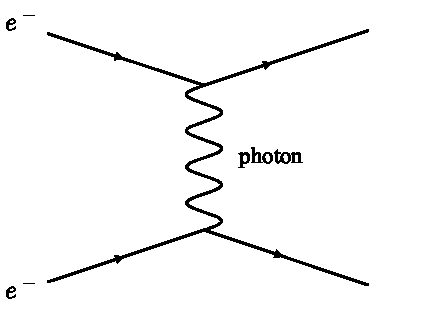
\includegraphics[width=0.72\textwidth]{fig_4.1.pdf}
\caption*{图 4.1\quad 电磁相互作用的 Feynman 图。在量子场论中，这类图被用来计算散射过程的振幅；在这里，只需把它当作表示某种相互作用的示意图即可。这张图的要点在于，光子与电子的耦合正是电子之间电磁相互作用的起因。与此相反，光子与其他光子之间没有耦合，也不存在光子之间相互作用的类似图形。}
\end{figure}

与此相反，不存在两个光子彼此之间交换另一个光子的图，因为电磁理论是线性的（没有反作用）。而引力相互作用则可以看成源于一个虚引力子（graviton，度规的量子化微扰）的交换。非线性表现为：电子与引力子都能交换虚引力子，从而产生引力，如图 4.2 所示。引力的这一特征并不独特；大多数规范理论都有它，例如作为强相互作用理论的量子色动力学（quantum chromodynamics）。电磁理论实际上是例外；其线性可以追溯到相关规范群 U(1) 是阿贝尔群这一事实。但非线性确实代表了对 Newton 理论的偏离。这一差异在实验上是可以检测的；（正如我们将看到的）水星轨道在 GR 中与在 Newton 引力中之所以不同，正是因为引力场会影响自身，而且越靠近太阳，这种影响就越明显。
% ---- 书页 167 / p182 ----
\begin{figure}[H]
\centering
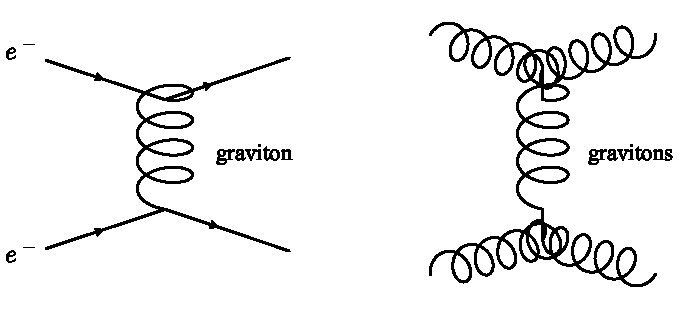
\includegraphics[width=0.72\textwidth]{fig_4.2.pdf}
\caption*{图 4.2\quad 引力的 Feynman 图。量子化之后，Einstein 方程预言自旋为 2 的粒子，称为引力子。我们尚不知道如何一致地完成这种量子化，但引力子的存在性足够稳固，被预期为任何良好定义的方案都会具有的特征。由于引力与能量-动量耦合，引力子与所有种类的粒子（包括其他引力子）都有相互作用。这为思考 Einstein 理论的非线性提供了一种方式。}
\end{figure}

除了复杂与非线性之外，还有一点值得思考：Einstein 方程究竟告诉了我们什么？显然，它把能量-动量分布与曲率张量的分量联系起来；但从物理的观点看，给定某种源，究竟会产生哪一种引力场？回答这个问题的一种方式，是考虑一族相邻类时测地线的\emph{膨胀}（expansion）$\theta$ 的演化。设想一小团自由检验粒子沿测地线运动，具有四速度 $U^\mu$，我们追踪它们的演化；膨胀 $\theta=\nabla_\mu U^\mu$ 告诉我们，这团粒子的体积在任一时刻是在增长（或在 $\theta<0$ 时收缩）。显然，膨胀的数值将依赖于检验粒子的初始条件。而引力的效应则编码在膨胀的\emph{演化}之中，后者由 Raychaudhuri 方程支配。这条在附录 F 中讨论的方程告诉我们，膨胀沿测地线对固有时 $\tau$ 的导数由下面的表达式给出：
\begin{equation*}
\frac{d\theta}{d\tau} = 2\omega^2 - 2\sigma^2 - \frac{1}{3}\theta^2 - R_{\mu\nu}U^\mu U^\nu.
\tag{4.81}
\end{equation*}
右边的各项在附录 F 中有仔细的解释；$\omega$ 编码测地线的转动，$\sigma$ 编码切变，而 $R_{\mu\nu}$ 当然就是 Ricci 张量。Raychaudhuri 方程是纯几何的关系，完全不涉及 Einstein 方程。然而，把两个方程结合起来，就可以描述能量-动量如何影响检验粒子的运动，因为 Einstein 方程把 $T_{\mu\nu}$ 与 $R_{\mu\nu}$ 联系起来，而 Raychaudhuri 方程把 $R_{\mu\nu}$ 与 $d\theta/d\tau$ 联系起来。
% ---- 书页 168 / p183 ----
让我们考虑最简单的情形：一开始，所有相邻粒子在时空的一个小区域内彼此相对静止。于是在这一初始时刻，膨胀、转动和切变全都为零。我们进一步构造局部惯性坐标系 $x^{\hat\mu}$，其中 $U^{\hat\mu}$ 处于其静止系，使得 $U^{\hat\mu}=(1,0,0,0)$，且 $R_{\hat\mu\hat\nu}U^{\hat\mu}U^{\hat\nu}=R_{\hat 0\hat 0}$。于是我们（在这组坐标下、在该点）有
\begin{equation*}
\frac{d\theta}{d\tau} = -R_{\hat 0\hat 0}.
\tag{4.82}
\end{equation*}
现在我们可以求助于如下形式的 Einstein 方程：
\begin{equation*}
R_{\mu\nu} = 8\pi G\left(T_{\mu\nu}-\frac{1}{2}Tg_{\mu\nu}\right).
\tag{4.83}
\end{equation*}
由于我们处在局部惯性坐标系中，所以有
\begin{align*}
g_{\hat\mu\hat\nu} &= \eta_{\hat\mu\hat\nu} \tag{4.84}\\
T &= g^{\hat\mu\hat\nu}T_{\hat\mu\hat\nu} = -\rho + p_x + p_y + p_z, \tag{4.85}
\end{align*}
其中 $\rho=T_{\hat 0\hat 0}$ 是静止系能量密度，而 $p_k=T_{\hat k\hat k}$ 是 $x^{\hat k}$ 方向上的压强。于是，式 (4.82) 变成
\begin{equation*}
\frac{d\theta}{d\tau} = -4\pi G(\rho + p_x + p_y + p_z).
\tag{4.86}
\end{equation*}
这个方程告诉我们：能量与压强产生一种引力场，它使初始静止的检验粒子团的体积趋于缩小（如果 $\rho$ 和各个 $p_i$ 都是正的）。换言之，引力是吸引的。

当然，从式 (4.86) 我们看到，引力并不\emph{必然}是吸引的；我们可以想象 $\rho+p_x+p_y+p_z$ 为负数的源。显然，压强所扮演的角色值得注意。一方面，它代表了对 Newton 理论毫不含糊的偏离——在 Newton 理论中压强不影响引力（它不出现在 Poisson 方程 $\nabla^2\Phi=4\pi G\rho$ 中）。这一差异在我们的太阳系里很难察觉，因为太阳和行星内部的压强远小于能量密度，而后者由组成粒子的静质量主导。另一方面，请注意压强的\emph{引力}效应与我们更熟悉的\emph{直接}效应正好相反——直接效应是正压强会把东西推开。在多数情形下，压强的直接效应要明显得多。然而，压强只有在存在压强梯度时才能直接起作用（例如活塞内外之间的压强差），而引力效应只依赖压强在当地的数值。如果压强完全平滑，它就只能通过其引力效应被探测到；真空能就是这样的一个例子，我们将在 4.5 节讨论它。
% ---- 书页 169 / p184 ----
关于式 (4.86) 最后再评论一点：它与 Einstein 方程完全等价——两者传达完全相同的信息。这个非常具体的关系对任何一组初始静止的检验粒子都成立；而它能成立的唯一途径，就是 Einstein 方程的所有分量都为真。因此，如果我们愿意，就可以用文字\footnote{J.C. Baez, “The Meaning of Einstein's Equation”〔“Einstein 方程的含义”〕， http://arXiv.org/abs/gr-qc/0103044.}把 Einstein 方程表述如下：“任何一组初始静止的粒子，其体积的膨胀正比于（负的）能量密度与三个压强分量之和。”

于是，Einstein 方程告诉我们，能量密度和压强以某种方式影响 Ricci 张量，使得当 $\rho$ 和 $p$ 为正时粒子相互吸引。那么，Riemann 张量中不包含在 Ricci 张量之内的那些分量呢？在第 3 章中我们发现，这些分量由 Weyl 张量描述（这里写出四维情形的表达式）：
\begin{equation*}
C_{\rho\sigma\mu\nu} = R_{\rho\sigma\mu\nu} + \frac{1}{3}g_{\rho[\mu}g_{\nu]\sigma}R - g_{\rho[\mu}R_{\nu]\sigma} + g_{\sigma[\mu}R_{\nu]\rho}.
\tag{4.87}
\end{equation*}
Ricci 张量是 Riemann 张量的迹，而 Weyl 张量描述其无迹部分；二者合起来完整地刻画了曲率。显然，给定某个确定的能量-动量分布，Weyl 曲率的选择仍有某种自由，因为没有类似 Einstein 方程的关系能把 $C^\rho{}_{\sigma\mu\nu}$ 与 $T_{\mu\nu}$ 代数地联系起来。而这正是理应如此。例如，设想一个处处真空的时空，$R_{\mu\nu}=0$。平直的 Minkowski 空间是这种情形下的一个可能解，但穿越空旷时空传播的引力波同样是可能的解（我们将在第 7 章讨论）。

既然进入 Einstein 方程的只有 $R_{\mu\nu}$，看起来 $C_{\rho\sigma\mu\nu}$ 的分量似乎完全不受约束。但请回忆，我们并不被允许在流形上任意指定曲率张量的分量；它们由 Bianchi 恒等式联系着，
\begin{equation*}
\nabla_{[\lambda}R_{\rho\sigma]\mu\nu} = 0.
\tag{4.88}
\end{equation*}
正如你在第 3 章习题 10 中证明过的，这个恒等式蕴含 Weyl 张量满足如下形式的微分关系：
\begin{equation*}
\nabla^\rho C_{\rho\sigma\mu\nu} = \nabla_{[\mu}R_{\nu]\sigma} + \frac{1}{6}g_{\sigma[\mu}\nabla_{\nu]}R.
\tag{4.89}
\end{equation*}
在右边，Riemann 张量只是通过它的缩并——Ricci 标量与 Ricci 张量——出现，而后者可以经由 Einstein 方程与 $T_{\mu\nu}$ 联系起来；于是我们有
\begin{equation*}
\nabla^\rho C_{\rho\sigma\mu\nu} = 8\pi G\left(\nabla_{[\mu}T_{\nu]\sigma} + \frac{1}{3}g_{\sigma[\mu}\nabla_{\nu]}T\right).
\tag{4.90}
\end{equation*}
因此，虽然 $R_{\mu\nu}$ 与 $T_{\mu\nu}$ 通过 Einstein 方程代数地相联系，$C_{\rho\sigma\mu\nu}$ 与 $T_{\mu\nu}$ 却是由这个一阶微分方程联系的。对一个给定的能量-动量分布，会存在若干可能的解，每个解由特定的边界条件确定。这个方程可以看成引力波的传播方程，与麦克斯韦方程组 $\nabla_\mu F^{\nu\mu}=J^\nu$ 极为类似。
% ---- 书页 170 / p185 ----
列举了 Einstein 方程这么多可爱的性质之后，似乎也应当公平地提一提它令人沮丧的一面：广为人知的、广义相对论与量子力学难以调和的困难。GR 是一个经典场论：动力学变量是定义在时空上的一个场（度规），由这个场构造出的坐标不变量（如标量曲率）原则上可以被任意精确地指定和测量。对于其他场论（如电磁学），从经典理论出发将其量子化、进而得到作用在 Hilbert 空间中的波函数之上的算符的动力学，有着理解透彻的成熟程序。而对 GR 来说，通常的程序会同时遭遇技术困难和概念困难，对此的描述超出了本书的范围。技术困难的一个方面是，GR 不像粒子物理的标准模型那样是“可重整化的”（renormalizable）；当考虑高阶量子效应时，会出现无法被任何有限多个参数吸收的无穷大。不可重整化并不意味着理论在根本上就是错的，但它强烈暗示，只应在某个能标以下才认真地对待这个理论。

幸运的是，量子引力的可观测效应预计要远离我们的日常经验（或者顺便说一句，也远离实验室中能实现的任何条件）才会变得重要。早在 1899 年，Planck 就注意到，他自己的常数 $h$——如今我们更常用 $\hbar = h/2\pi = 1.05\times10^{-27}\,\mathrm{cm}^2\,\mathrm{g/sec}$ 来代替它——可以与 Newton 引力常数 $G = 6.67\times10^{-8}\,\mathrm{cm}^3\,\mathrm{g}^{-1}\,\mathrm{sec}^{-2}$ 以及光速 $c = 3.00\times10^{10}\,\mathrm{cm}\,\mathrm{sec}^{-1}$ 组合起来，构成一组基本的带量纲的量：Planck 质量
\begin{equation*}
m_{\mathrm{P}} = \left(\frac{\hbar c}{G}\right)^{1/2} = 2.18\times 10^{-5}\,\mathrm{g},
\tag{4.91}
\end{equation*}
Planck 长度
\begin{equation*}
l_{\mathrm{P}} = \left(\frac{\hbar G}{c^3}\right)^{1/2} = 1.62\times 10^{-33}\,\mathrm{cm},
\tag{4.92}
\end{equation*}
Planck 时间
\begin{equation*}
t_{\mathrm{P}} = \left(\frac{\hbar G}{c^5}\right)^{1/2} = 5.39\times 10^{-44}\,\mathrm{sec},
\tag{4.93}
\end{equation*}
以及 Planck 能量
\begin{align*}
E_{\mathrm{P}} &= \left(\frac{\hbar c^5}{G}\right)^{1/2} = 1.95\times 10^{16}\,\mathrm{erg} \tag{4.94}\\
&= 1.22\times 10^{19}\,\mathrm{GeV}. \tag{4.95}
\end{align*}
% ---- 书页 171 / p186 ----
一个 GeV 是 $10^9$ 电子伏特，它是粒子物理中的常用单位，因为它大约是一个质子的质量。我们通常取 $\hbar = c = 1$，于是这些量就变得无从区分，即 $m_{\mathrm{P}} = l_{\mathrm{P}}^{-1} = t_{\mathrm{P}}^{-1} = E_{\mathrm{P}}$。你会听到人们说诸如“Planck 质量是 $10^{19}$ GeV”之类的话，或者干脆说“Planck 标度”（Planck scale）。另一个常用量是约化 Planck 标度（reduced Planck scale）$\bar{m}_{\mathrm{P}} = m_{\mathrm{P}}/\sqrt{8\pi} = 2.43\times10^{18}\,\mathrm{GeV}$，它在方程中往往更加方便——注意式 (4.73) 中标量曲率的系数正是 $\bar{m}_{\mathrm{P}}^2/2$。很可能，只有当我们考虑的粒子质量大于 $m_{\mathrm{P}}$、时间短于 $t_{\mathrm{P}}$、长度小于 $l_{\mathrm{P}}$、或能量高于 $E_{\mathrm{P}}$ 时，量子引力才变得重要；在更低的标度下，经典 GR 就应当足够了。由于这些都远离可观测的现象，构造一个自洽的量子引力理论更多是一个原则问题，而非实际问题。另一方面，弯曲时空中的量子效应在现实世界中可能很重要；正如我们将在第 8 章讨论的，它们可能导致早期宇宙中的密度涨落，而这些涨落会成长为今天我们观测到的星系和大尺度结构。

在完全量子的理论中，有一个在适当极限下能涵盖 GR 的领先候选者：弦论（string theory）。在弦论中，我们设想基本的对象不是像电子或光子那样的点粒子，而是被称为弦的细小的一维对象，它们既可以是闭合的圈，也可以是开放的线段。弦论最初是作为强核力的模型被提出的，但人们很快意识到，该理论不可避免地预言了一个无质量的自旋 2 粒子：这恰恰是一个量子引力理论所需要的东西。弦论看起来是一个自洽的量子理论，而且它预言了引力，但关于它仍有许多我们不理解的地方。特别是，经典时空如何从基本的弦之中产生，这一点颇为神秘；而它与直接实验的联系，充其量也十分微弱。尽管如此，弦论异常丰富而强健，有望在可预见的未来成为理论物理的重要部分。

\section{宇宙学常数}

广义相对论的一个特征是，引力场的源是整个能动张量。在非引力的物理中，只有能量从一个态到另一个态的\emph{改变}才是可测的；能量的归一化是任意的。例如，势能为 $V(x)$ 的粒子的运动，与势能为 $V(x)+V_0$ 的粒子的运动完全相同，其中 $V_0$ 是任意常数。然而在引力中，能量的实际数值是重要的，而不仅仅是态之间的差。

这种行为开启了\textbf{真空能}（vacuum energy）的可能性：一种为空的空间所特有的能量密度。我们或许希望真空具备的一个特征是：它不挑出任何一个特殊的方向；只要相应的能动张量在局部惯性坐标系中是洛伦兹不变的，非零的能量密度就仍然是可能的。洛伦兹不变性意味着相应的能动张量应当正比于度规：
% ---- 书页 172 / p187 ----
\begin{equation*}
T^{(\mathrm{vac})}_{\hat\mu\hat\nu} = -\rho_{\mathrm{vac}}\,\eta_{\hat\mu\hat\nu},
\tag{4.96}
\end{equation*}
因为 $\eta_{\hat\mu\hat\nu}$ 是唯一的洛伦兹不变 (0,2) 型张量。这可以直截了当地从惯性坐标推广到任意坐标：
\begin{equation*}
T^{(\mathrm{vac})}_{\mu\nu} = -\rho_{\mathrm{vac}}\,g_{\mu\nu}.
\tag{4.97}
\end{equation*}
与理想流体的能动张量 $T_{\mu\nu}=(\rho+p)U_\mu U_\nu + pg_{\mu\nu}$ 相比较，我们发现真空看起来像一种理想流体，其各向同性的压强与能量密度符号相反：
\begin{equation*}
p_{\mathrm{vac}} = -\rho_{\mathrm{vac}}.
\tag{4.98}
\end{equation*}
能量密度应当在整个时空中为常数，因为若有梯度就不再是洛伦兹不变的了。

如果我们把能动张量分解为物质部分 $T^{(\mathrm{M})}_{\mu\nu}$ 与真空部分 $T^{(\mathrm{vac})}_{\mu\nu}=-\rho_{\mathrm{vac}}g_{\mu\nu}$，Einstein 方程就是
\begin{equation*}
R_{\mu\nu}-\frac{1}{2}Rg_{\mu\nu} = 8\pi G\left(T^{(\mathrm{M})}_{\mu\nu}-\rho_{\mathrm{vac}}g_{\mu\nu}\right).
\tag{4.99}
\end{equation*}
在发明 GR 之后不久，Einstein 试图寻找一个静态的宇宙学模型，因为当时的天文观测似乎正暗示这一点。其结果就是 Einstein 静态宇宙，我们将在第 8 章讨论它。为了让这个静态宇宙学在普通物质源之下求解场方程，有必要添加一个称为\textbf{宇宙学常数}（cosmological constant）的新项 $\Lambda$，它以如下方式进入：
\begin{equation*}
R_{\mu\nu}-\frac{1}{2}Rg_{\mu\nu} + \Lambda g_{\mu\nu} = 8\pi G T_{\mu\nu}.
\tag{4.100}
\end{equation*}
与式 (4.99) 比较可见，宇宙学常数恰恰等价于引入一个真空能密度
\begin{equation*}
\rho_{\mathrm{vac}} = \frac{\Lambda}{8\pi G}.
\tag{4.101}
\end{equation*}
“宇宙学常数”与“真空能”这两个术语实质上可以互换。

非零的真空能是我们应当预期的东西吗？我们当初是通过寻找能从度规构造出的最简单的标量，而得到 Hilbert 拉格朗日量 $\widehat{\mathcal{L}}_H = R$ 的。当然，还有一个更简单的候选，即常数。利用式 (4.69)，不难检验
\begin{equation*}
S = \int d^4x\sqrt{-g}\left[\frac{1}{16\pi G}(R-2\Lambda) + \widehat{\mathcal{L}}_{\mathrm{M}}\right]
\tag{4.102}
\end{equation*}
% ---- 书页 173 / p188 ----
会导致修改后的方程 (4.100)；或者换个说法，真空的拉格朗日量就是
\begin{equation*}
\widehat{\mathcal{L}}_{\mathrm{vac}} = -\rho_{\mathrm{vac}}.
\tag{4.103}
\end{equation*}
所以，引入真空能当然容易；然而，对它的预期取值我们毫无洞察，因为它以一个任意常数的形式进入。

真空能归根结底本身就是自然界的一个常数。（在某些理论中会出现例外：某个时空对称性——例如超对称性或共形不变性——支配着真空能的取值；这里我们考虑的是更一般的场论。）尽管如此，真空能有各种各样不同的贡献来源，如果总取值远小于各个单独的贡献，那就奇怪了。其中一种贡献来自零点涨落（zero-point fluctuations）——量子场处于真空态时的能量。

考虑一个简谐振子，即在一维势 $V(x)=\frac{1}{2}\omega^2 x^2$ 中运动的一个粒子。经典地看，这个系统的真空是粒子静止于势的极小值处（$x=0$）的态，此时能量为零。然而从量子力学上看，不确定性原理不允许我们同时确定粒子的位置和动量，我们会发现最低能量态具有能量 $E_0=\frac{1}{2}\hbar\omega$（这里为了清晰起见，我们临时重新引入了显式的 $\hbar$ 因子）。当然，在没有引力时，无论哪个系统，其真空能实际上都是完全任意的；我们可以给势加上任何常数而不改变理论。但量子涨落已经使零点能不同于我们的经典预期。

在场论中有一个完全类似的情形。如果我们对一个自由量子场（为简单起见忽略相互作用的场）做傅里叶变换，就会发现它变成动量空间中无穷多个谐振子，正如我们将在第 9 章讨论的。每个振子的频率为 $\omega=\sqrt{m^2+k^2}$，其中 $m$ 是场的质量，$k$ 是该模式波矢的大小。如果我们把经典真空能取为零，这些模式中的每一个都贡献一份量子零点能 $\hbar\omega/2$。形式上，把所有这些贡献加起来会得到一个无穷大的结果。然而，如果我们以“只在某个紫外动量截断 $k_{\mathrm{max}}$ 以下才信任我们的理论”为由，丢弃动量非常高的那些模式，就会发现所得的能量密度具有如下形式：
\begin{equation*}
\rho_{\mathrm{vac}} \sim \hbar k_{\mathrm{max}}^4.
\tag{4.104}
\end{equation*}
这个答案本来可以靠量纲分析猜出来；被略去的数值常数将依赖于所考虑的具体理论。如果我们有信心把普通量子场论一直用到约化 Planck 标度 $\bar{m}_{\mathrm{P}} = (8\pi G)^{-1/2} \sim 10^{18}\,\mathrm{GeV}$，我们预计会有一个量级为
\begin{equation*}
\rho_{\mathrm{vac}} \sim (10^{18}\,\mathrm{GeV})^4 \sim 10^{112}\,\mathrm{erg/cm^3}.
\tag{4.105}
\end{equation*}
% ---- 书页 174 / p189 ----
的贡献。场论也可能更早就失效，不过，要相信它会在任何具体的标度上失效，量子引力是我们所拥有的最好的理由。

正如我们将在第 8 章讨论的，宇宙学观测意味着
\begin{equation*}
\left|\rho^{(\mathrm{obs})}_{\Lambda}\right| \leq (10^{-12}\,\mathrm{GeV})^4 \sim 10^{-8}\,\mathrm{erg/cm^3},
\tag{4.106}
\end{equation*}
这比刚才导出的朴素预期小得多。式 (4.105) 与式 (4.106) 之比，正是宇宙学常数的理论值与观测值之间那著名的 120 个数量级差异的由来。我们可以随意设想裸真空能经过调整，使得净宇宙学常数与极限 (4.106) 相符；但有一个问题：我们不知道有任何特殊的对称性，既能强制真空能为零，又与已知的物理定律相容；这个难题就是“宇宙学常数问题”（cosmological constant problem）。我们将在第 8 章更多地讨论真空能的宇宙学效应。\footnote{关于真空能的物理与宇宙学的更多内容，见 S.M. Carroll, \emph{Liv. Rev. Rel.} \textbf{4}, 1 (2001), http://arxiv.org/astro-ph/0004075.}

\section{能量条件}

有时，不指明 $T_{\mu\nu}$ 由哪一种物质理论导出，而去思考 Einstein 方程，是有用的。这会给我们留下极大的任意性；例如考虑这样一个问题：哪些度规服从 Einstein 方程？在没有对 $T_{\mu\nu}$ 的某些约束时，答案是任何度规都行；只需取你喜欢的度规，为它算出 Einstein 张量 $G_{\mu\nu}$，然后要求 $T_{\mu\nu}$ 等于 $G_{\mu\nu}$ 即可。而由 Bianchi 恒等式，它自动守恒。我们真正关心的，是在“现实的”（realistic）能量与动量源——姑且不论这个词是什么意思——存在时 Einstein 方程解的存在性。一种策略是考虑具体的源，比如标量场、尘埃或电磁场。然而，我们有时希望理解的是那些对各种不同源都成立的 Einstein 方程的性质。在这种情况下，方便的做法是施加\emph{能量条件}（energy conditions）来限制 $T_{\mu\nu}$ 的任意性。

能量条件是对能动张量的坐标不变的限制。因此我们必须从 $T_{\mu\nu}$ 构造标量，这通常通过把它与任意的类时矢量 $t^\mu$ 或类光矢量 $\ell^\mu$ 缩并来实现。例如，弱能量条件（weak energy condition, WEC）陈述：对所有类时矢量 $t^\mu$，都有 $T_{\mu\nu}t^\mu t^\nu\geq 0$。为了建立物理直觉，考虑源为理想流体的特殊情形是有用的，此时能动张量取如下形式：
\begin{equation*}
T_{\mu\nu} = (\rho + p)U_\mu U_\nu + pg_{\mu\nu},
\tag{4.107}
\end{equation*}
其中 $U^\mu$ 是流体的四速度。让我们用这个形式把 WEC 翻译成物理的语言。由于压强是各向同性的，只要对某个类光矢量 $\ell^\mu$，$T_{\mu\nu}U^\mu U^\nu \geq 0$ 与 $T_{\mu\nu}\ell^\mu\ell^\nu \geq 0$ 同时成立，
% 本块末句在原书书页174底部中断（“will be nonnegative”续接书页175顶部 “for all timelike vectors t^mu if both T_{mu nu}U^mu U^nu >= 0 and ...”），下一块请用 %JOIN% 续接本句。
$T_{\mu\nu}t^\mu t^\nu$ 就对所有类时矢量 $t^\mu$ 非负（请自己验证这一点；这不过是矢量相加而已）。因此我们来计算
\begin{equation*}
T_{\mu\nu}U^\mu U^\nu = \rho, \qquad T_{\mu\nu}\ell^\mu\ell^\nu = (\rho + p)(U_\mu \ell^\mu)^2.
\tag{4.108}
\end{equation*}
因此 WEC 意味着 $\rho \geq 0$ 和 $\rho + p \geq 0$。这些听起来都十分合理：能量密度非负，并且压强相对于能量密度不能太大。当然，我们不必把自己限制在理想流体上，我们只是利用它们来洞察能量条件所施加的要求。

能量条件有许多种，各自适用于不同的情形。下面是一些最常见的：

\begin{itemize}
\item \textbf{弱能量条件}（Weak Energy Condition），或称 WEC，正如刚才讨论的，它要求对所有类时矢量 $t^\mu$ 有 $T_{\mu\nu}t^\mu t^\nu \geq 0$，或者等价地，$\rho \geq 0$ 且 $\rho + p \geq 0$。

\item \textbf{类光能量条件}（Null Energy Condition），或称 NEC，要求对所有类光矢量 $\ell^\mu$ 有 $T_{\mu\nu}\ell^\mu\ell^\nu \geq 0$，或者等价地，$\rho + p \geq 0$。它是 WEC 的特例，只是把类时矢量换成了类光矢量。此时能量密度可以取负值，只要存在补偿性的正压强。

\item \textbf{主能量条件}（Dominant Energy Condition），或称 DEC，包含 WEC（对所有类时矢量 $t^\mu$ 有 $T_{\mu\nu}t^\mu t^\nu \geq 0$），外加一条附加要求：$T^\mu{}_\nu t^\nu$ 是非类空（nonspacelike）矢量（也就是说，$T_{\mu\nu}T^\nu{}_\lambda t^\mu t^\lambda \leq 0$）。对于理想流体，这些条件合在一起等价于一个简单的要求：$\rho \geq |p|$；能量密度必须非负，并且不小于压强的大小。

\item \textbf{类光主能量条件}（Null Dominant Energy Condition），或称 NDEC，是仅对类光矢量成立的 DEC 条件：对任意类光矢量 $\ell^\mu$，$T_{\mu\nu}\ell^\mu\ell^\nu \geq 0$，并且 $T^\mu{}_\nu \ell^\nu$ 是非类空矢量。允许的密度和压强与 DEC 相同，只是允许负密度，只要 $p = -\rho$。换句话说，凡是会被 DEC 排除的源，NDEC 同样排除——负真空能除外。

\item \textbf{强能量条件}（Strong Energy Condition），或称 SEC，要求对所有类时矢量 $t^\mu$ 有 $T_{\mu\nu}t^\mu t^\nu \geq \frac{1}{2}T^\lambda{}_\lambda t^\sigma t_\sigma$，或者等价地，$\rho + p \geq 0$ 且 $\rho + 3p \geq 0$。注意 SEC 并\emph{不}蕴含 WEC。它蕴含 NEC，同时还排除了过大的负压强。从式 (4.86) 我们看到，正是 SEC 意味着引力是吸引的。
\end{itemize}

这些条件在图 4.3 中给出了解示。此外我们还画出了约束 $w \geq -1$，其中 $w = p/\rho$ 被称为\textbf{物态方程参数}（equation-of-state parameter）。这是宇宙学中一个有用的概念，因为宇宙学中的源常常具有 $p = w\rho$ 形式的物态方程，其中 $w$ 为常数（当然，无论 $w$ 是不是常数，它都是有定义的）。如果我们把自己限制在 $\rho \geq 0$ 的源，那么上述任何一个能量条件都将蕴含 $w \geq -1$。

\begin{figure}[H]
\centering
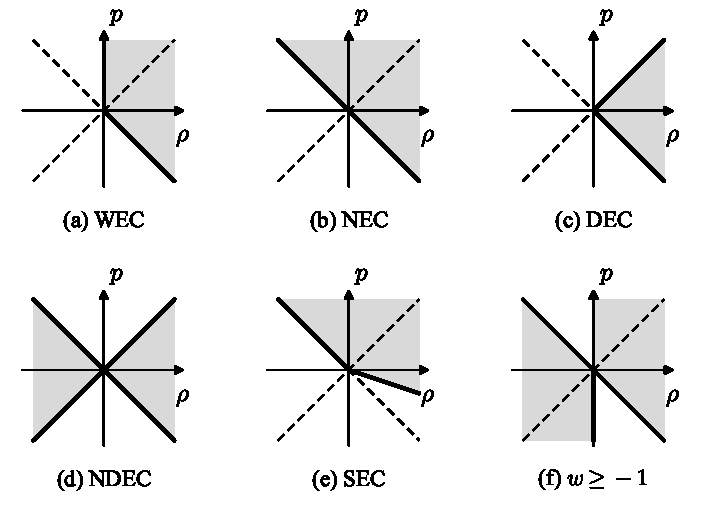
\includegraphics[width=0.72\textwidth]{fig_4.3.pdf}
\caption*{图 4.3\quad 能量条件应用于理想流体的情形，表示为能量密度 $\rho$ 与压强 $p$ 平面上的允许区域。图中画出了弱能量条件（WEC）、类光能量条件（NEC）、主能量条件（DEC）、类光主能量条件（NDEC）以及强能量条件（SEC）。作为比较，我们还画出了条件 $w \geq -1$，其中 $w = p/\rho$ 为物态方程参数。}
\end{figure}

大多数普通的经典物质形式，包括标量场和电磁场，都遵守 DEC（见习题），因而也遵守限制较弱的条件（WEC、NEC、NDEC）。SEC 在某些奇点定理的证明中很有用，但可以被某些形式的物质破坏，例如有质量的标量场。事实证明，量子场通常能够破坏我们列出的任何一种能量条件；不过，也可能存在一些涉及时空区域上积分的不等式，即使是量子场也满足它们。这是目前仍在活跃研究的一个领域。

严格说来，能量条件与能量守恒并没有关系；无论我们对 $T^{\mu\nu}$ 施加什么附加约束，Bianchi 恒等式都保证 $\nabla_\mu T^{\mu\nu} = 0$。它们的作用在于防止其他被我们视为“非物理”的性质，例如能量以超过光速的速度传播，或者空的空间自发衰变为正负能量互相补偿的区域。特别是，Hawking 和 Ellis (1973) 证明了一个\emph{守恒定理}（conservation theorem）：大致说来，如果能动张量遵守 DEC，并且在某个类空区域中为零，那么它必定在该区域的未来依赖域中处处为零（未来依赖域的定义见 2.7 节）。这样一来，能量不可能无中生有地冒出来，也不可能溜到光锥之外。该定理并不包括其逆命题（即违反 DEC 的源必然是非因果的），所以谨慎一点总是有好处的。

\section{再论等效原理}

本节我们将更仔细地考察等效原理的依据和后果，我们在 4.1 节中曾用它来启发把物理学推广到弯曲时空的最小耦合步骤。我们将看到，等效原理并不是一条神圣的物理定律，甚至算不上一个数学上严格的陈述；在更基本的层次上，它的产生是广义相对论作为一种在宏观距离上有效的有效场论这一本质的结果，而我们的任务则是确定在这样的理论中，我们应当预期物质与度规之间存在哪些类型的耦合。

在实践中，人们常常援引等效原理来为下面四种观念中的任何一种辩护：
\begin{enumerate}
\item 物理学定律应当（或至少可以）以广义协变的形式表述。
\item 时空中存在一个度规，其曲率被我们解释为引力。
\item 不存在任何其他与引力相像的场。
\item 物质场与曲率的相互作用是最小的：它们不包含与 Riemann 张量或其缩并的直接耦合。
\end{enumerate}

这些截然不同的陈述，各自有着非常不同的地位：第一种是空洞的，第二种既深刻又几乎肯定为真，第三种有趣且可检验，而第四种只不过是一个有用的近似。让我们逐一考察。

第一种陈述有时被称为\textbf{协变性原理}（Principle of Covariance）。它多少是没什么内容的。“广义协变”只是说，方程中所有的项在坐标变换下以相同的方式变换，从而方程的形式是坐标不变的。由于张量变换规律的普适性，实现这一目标最直接的办法，就是把方程写成明显的张量形式。当然，一条定律若以并非广义协变的形式表述，也没有任何问题，只要我们知道能够把它改写成与坐标无关的形式。另一方面，只要定律从一开始就是良定义的，把它写成与坐标无关的形式总是\emph{可能的}。一个以某种方式行为的物理系统，并不知道你正在用哪个坐标系来描述它；因此，任何配得上“物理学定律”这一名称的东西（相对于该定律的某个特定表述而言）都必定与坐标无关。坚持显式的坐标不变性，对于定律如何向弯曲时空推广并没有说什么；正如我们已看到的，明显的张量方程不论几何如何都取相同的形式。

考虑平直时空中的麦克斯韦方程组，如同我们在第 1 章中写下的那样：
\begin{equation*}
\partial_\mu F^{\nu\mu} = J^\nu.
\tag{4.109}
\end{equation*}
右边是一个良定义的张量，而左边由于出现了偏导数则不是。这没有问题，因为我们知道这个方程只在 Minkowski 空间的惯性坐标中有效。用坐标不变的方式表达同一定律，则是
\begin{equation*}
\nabla_\mu F^{\nu\mu} = J^\nu.
\tag{4.110}
\end{equation*}
要断言这就是 Minkowski 空间中正确的表述，无需援引任何物理原理；它是\emph{唯一的}张量方程，在惯性坐标中与式 (4.109) 等价。但它并不是向弯曲时空的唯一推广，因为我们可以想象一些新的项，涉及 $F_{\mu\nu}$ 与 $R^\rho{}_{\sigma\mu\nu}$ 的乘积；这类附加项的地位由最小耦合假设直接处理，即上面清单中的第四点。不过，“把东西弄成张量的”或“广义协变的”这件事本身，只是逻辑必然性的简单体现，并不是一个可以设想用实验来否证的物理原理。（同一思想的另一种说法是“微分同胚不变性”（diffeomorphism invariance），在附录 B 中讨论。）

上面清单中，等效原理的第二条所谓后果要深刻得多，而且绝非显然。虽然 Einstein 是受 EP 的启发，但这一几何洞见正是他的伟大突破。在第 2 章开头我们讨论过为什么这样的洞见是有根据的：EP 意味着引力是普适的，这又进而意味着引力场在小的时空区域内变得无法测量，而这一特征最直接的实现方式，就是把引力与时空几何的效应等同起来。这些步骤是有充分动机的建议，而不是严格推导出的结论；一旦我们有了“存在一个度规、其曲率产生引力”的想法，就可以通过与实验比较来检验它的用处。正如我们提到的，它以优异的成绩通过了检验。不断积累的证据（例如第 2 章讨论过的引力红移）与“理想化的直尺和时钟，其表现正如时空几何弯曲时应有的表现”这一想法相一致。尽管如此，不应指望去证明真的存在一个具有所期望性质的度规；我们提出假设，用越来越精确的实验去检验它，并推断它的适用范围。的确，最终调和广义相对论与量子力学的要求，让许多人相信度规终将被揭示为一个由更基本的一组自由度衍生出来的概念。就我们当前的目的而言，这个终极答案并不重要；弯曲度规这一想法的有用性已经被证明得无可置疑，我们要做的，是扩展对其性质的理解，直到碰上不可逾越的障碍（无论是理论上的还是经验上的）。

既然我们确信引力的效应最好归因于时空度规的曲率，那么如果实验探测到对等效原理的明显违反，我们会得出什么结论？例如，我们可能设想这样一个实验，它揭示检验物体朝向地球或太阳的加速度确实极其轻微地依赖于检验物体的成分。（目前对这类反常加速度最好的限制表明，它们小于引力所致加速度的 $10^{-12}$ 倍。）\footnote{Y.~Su et al., \emph{Phys. Rev.} \textbf{D~50}, 3614 (1994).} 在这种情况下，没有人会真的倾向于宣称广义相对论已被彻底推翻、有必要从头再来。更可能的做法是回到“检验物体”（test body）的定义上去，这个定义包含该物体不带电荷这一条件。举例来说，电子就不是一个好的检验物体，因为它除了受引力作用之外，还会被周围环境中的电磁场推来搡去。类似地，对于号称中性的检验物体上任何假想的反常加速度，迄今为止最直接的解释莫过于设想我们发现了一种新的长程场的存在，而我们的检验物体在这种场下其实是带荷的。这样的场要一直未被发现至今，它必须要么耦合极弱，要么必须近乎普适地耦合，以便模仿引力的效应。我们可以设想，比如，与能动张量的迹耦合的标量场，或者与重子数（baryon number）耦合的矢量场。普通检验物体的质量近似正比于其重子数，重子数计数的正是物体中质子和中子的数目。因此，有时把“等效原理的检验”方便地当作对我们上述第三条陈述的检验——即不存在任何其他与引力相像的场（如果一个场是长程的，并且近乎普适地与质量耦合，它就与引力相像）。同样，探测到对这一假设的违反，最直接的解释将是发现了一种新的“第五种力”（fifth force），而不是对 Einstein 思想的否定。至于如果我们改进现有实验，是否应当预期会发现这样一种新场，这很难说；一方面，随手就能构造出带有新长程力的模型，但另一方面，它们通常应当强到早已被探测到了。在这个阶段，保持开放的头脑仍然是值得的。

除了度规的存在本身之外，等效原理的核心在于我们表述中的第四条：物质场与曲率的相互作用是最小的，不包含与 Riemann 张量或其缩并的直接耦合。例如，我们可以考虑如下这个取代常规测地线方程的可能替代：
\begin{equation*}
\frac{d^2x^\mu}{d\lambda^2} + \Gamma^\mu_{\rho\sigma}\frac{dx^\rho}{d\lambda}\frac{dx^\sigma}{d\lambda} = \alpha\left(\nabla_\sigma R\right)\frac{dx^\mu}{d\lambda}\frac{dx^\sigma}{d\lambda},
\tag{4.111}
\end{equation*}
其中 $R$ 是 Ricci 标量曲率，$\alpha$ 是一个耦合常数。这个方程在平直时空中同样约化为直线运动，但通过测量与 $\nabla_\sigma R$ 的耦合，它将允许在小区域内直接探测时空曲率。那么，为什么大自然选择了简单的测地线方程呢？作为回答的第一步，考虑耦合 $\alpha$ 的量纲。由于 $c = 1$ 且空间和时间有相同的单位，我们可以用长度作为基本量纲。于是度规、逆度规以及 $dx^\mu/d\lambda$ 都是无量纲的。偏导数算符的单位是逆长度，协变导数也一样。Christoffel 符号包含度规的一阶导数，因此具有逆长度的量纲；类似地，Riemann 张量、Ricci 张量和 Ricci 标量曲率具有逆长度平方的量纲：
\begin{equation*}
\Big[\frac{dx^\mu}{d\lambda}\Big] = [g_{\mu\nu}] = [g^{\mu\nu}] = L^0, \qquad [\nabla_\mu] = [\Gamma^\mu_{\rho\sigma}] = L^{-1}, \qquad [R] = L^{-2}.
\tag{4.112}
\end{equation*}
为保持一致，耦合 $\alpha$ 必须具有长度平方的量纲：
\begin{equation*}
[\alpha] = L^2.
\tag{4.113}
\end{equation*}
因此 $\alpha$ 的平方根定义了一个长度尺度；这个长度尺度应当是多大？我们无法确定，但有充分的理由相信它应当极其小。有两点论证。其一，由于 $\alpha$ 所代表的耦合起源于引力，对相关长度尺度唯一合理的预期是
\begin{equation*}
\alpha \sim l_{\rm P}^2,
\tag{4.114}
\end{equation*}
其中 $l_{\rm P}$ 是 Planck 长度。另一个理由不过是“不然还能是什么呢”这种理由的更精致版本。虽然广义相对论是一个经典理论，但在更深的层次上，我们预期它只不过是描述某个底层量子力学结构的有效场论。即使不知道这个结构可能是什么，一个一般的预期（源自我们对已经理解的量子场论的经验）是：有效的经典极限应当包含所有可能的相互作用，只是带有量纲的长度参数，它们代表着新自由度开始变得重要的尺度（回忆第 1 章末尾我们对有效场论的讨论）。这样，弱相互作用的 Fermi 理论包含一个长度尺度，我们现在知道它对应于电弱对称性破缺的尺度，W 和 Z 玻色子在那里开始变得相关。既然我们不预期新的引力物理在 Planck 标度之前出现，与引力相伴的高阶相互作用就应当被 Planck 长度的适当幂次压低。

这代表着多大的压低？一种量度是将 $l_{\rm P}$（从而参数 $\alpha$ 可能的取值）与地球附近典型的引力长度尺度相比较。地球上引力的强度由重力加速度表征，$a_g = 980\ \mathrm{cm/sec^2}$。为构造一个具有长度量纲的量，我们定义
\begin{equation*}
l_\oplus = c^2/a_g \sim 10^{18}\ \mathrm{cm},
\tag{4.115}
\end{equation*}
其中符号 $\oplus$ 在这里代表地球（而不是直和）。于是，高阶引力效应的相对强度由下式量度：
\begin{equation*}
\frac{l_{\rm P}}{l_\oplus} \sim 10^{-51}.
\tag{4.116}
\end{equation*}
实际上，由于我们预期 $\alpha \sim l_{\rm P}^2$，压低将是 $10^{-102}$ 的量级。因此，似乎没什么必要担心这类耦合可能起的作用。但剧烈的偏离应当记在心里；近来关于大额外维的想法已经开启了在粒子加速器上观测直接引力相互作用的可能性。归根结底，没有办法仅仅靠纯粹的思考来解决这些问题；只有实验才能在各种替代方案中作出裁决。

\section{替代理论}

广义相对论已经通过了各种各样的实验检验。尽管如此，我们做的下一个实验仍有可能揭示对 Einstein 原始表述的偏离。因此，让我们简要考虑广义相对论可能被修改的几种方式。这样的方式多得不可胜数，但我们将考虑四种不同的可能性：
\begin{itemize}
\item 引力标量场
\item 额外空间维度
\item 作用量中的高阶项
\item 非 Christoffel 联络
\end{itemize}

一类流行的替代模型被称为引力\textbf{标量-张量理论}（scalar-tensor theories），因为它们同时涉及度规张量 $g_{\mu\nu}$ 和一个标量场 $\lambda$。特别地，标量场直接与标量曲率耦合，而不只是与度规耦合（正如等效原理似乎所蕴含的那样）。作用量可以写成引力部分、纯标量部分和物质部分之和：
\begin{equation*}
S = S_{fR} + S_\lambda + S_{\rm M},
\tag{4.117}
\end{equation*}
其中
\begin{equation*}
S_{fR} = \int d^4x\,\sqrt{-g}\, f(\lambda)R,
\tag{4.118}
\end{equation*}
\begin{equation*}
S_\lambda = \int d^4x\,\sqrt{-g}\left[-\frac{1}{2}h(\lambda)g^{\mu\nu}(\partial_\mu\lambda)(\partial_\nu\lambda) - U(\lambda)\right],
\tag{4.119}
\end{equation*}
以及
\begin{equation*}
S_{\rm M} = \int d^4x\,\sqrt{-g}\,\widehat{\mathcal{L}}_{\rm M}(g_{\mu\nu}, \psi_i).
\tag{4.120}
\end{equation*}
这里，$f(\lambda)$、$h(\lambda)$ 和 $U(\lambda)$ 是定义该理论的函数，而物质拉格朗日量 $\widehat{\mathcal{L}}_{\rm M}$ 依赖于度规和一组物质场 $\psi_i$，但不依赖于 $\lambda$。通过变量的改变，我们总可以令 $h(\lambda) = 1$，但我们把它保留在此，以便与文献中的模型进行比较。

这个理论的运动方程包括引力方程（由对度规变分得到）、标量方程（由对 $\lambda$ 变分得到），以及相应的物质方程。让我们从引力方程开始，我们可以按照与普通 Hilbert 作用量 (4.55) 相同的步骤来推导它。考虑度规的微扰
\begin{equation*}
g^{\mu\nu} \to g^{\mu\nu} + \delta g^{\mu\nu}.
\tag{4.121}
\end{equation*}
按照 4.3 节的步骤，作用量引力部分的变分为
\begin{align*}
\delta S_{fR} = {}& \int d^4x\,\sqrt{-g}\, f(\lambda)\Big[\Big(R_{\mu\nu} - \frac{1}{2}Rg_{\mu\nu}\Big)\delta g^{\mu\nu} + \nabla_\sigma\nabla^\sigma(g_{\mu\nu}\delta g^{\mu\nu}) \\
&- \nabla_\mu\nabla_\nu(\delta g^{\mu\nu})\Big].
\tag{4.122}
\end{align*}
对于 Hilbert 作用量，$f$ 是常数，所以最后两项是全导数，可以通过分部积分化为表面项从而忽略。现在，分部积分（两次）会得到 $f$ 的导数，我们便得出
\begin{equation*}
\delta S_{fR} = \int d^4x\,\sqrt{-g}\,\big[f(\lambda)G_{\mu\nu} + g_{\mu\nu}\Box f - \nabla_\mu\nabla_\nu f\big]\delta g^{\mu\nu},
\tag{4.123}
\end{equation*}
其中 $G_{\mu\nu}$ 是 Einstein 张量。我们像往常一样丢弃了表面项，尽管在这种情形下关于边界贡献有一些微妙之处；讨论见 Wald (1984)。于是，包含来自 $S_\lambda$ 和 $S_{\rm M}$ 的贡献的引力运动方程为
\begin{equation*}
G_{\mu\nu} = f^{-1}(\lambda)\left(\frac{1}{2}T^{({\rm M})}_{\mu\nu} + \frac{1}{2}T^{(\lambda)}_{\mu\nu} + \nabla_\mu\nabla_\nu f - g_{\mu\nu}\Box f\right),
\tag{4.124}
\end{equation*}
其中能动张量为 $T^{(i)}_{\mu\nu} = -2(-g)^{-1/2}\delta S_i/\delta g^{\mu\nu}$；特别地，
\begin{equation*}
T^{(\lambda)}_{\mu\nu} = h(\lambda)\nabla_\mu\lambda\nabla_\nu\lambda - g_{\mu\nu}\left[\frac{1}{2}h(\lambda)g^{\rho\sigma}\nabla_\rho\lambda\nabla_\sigma\lambda + U(\lambda)\right].
\tag{4.125}
\end{equation*}
观察式 (4.124) 中 $T^{({\rm M})}_{\mu\nu}$ 的系数可以看到，当标量场\emph{恒定}（或实际上如此）时，我们可以把 $f(\lambda)$ 认作 $1/(16\pi G)$，这从原始作用量 (4.118) 看是合理的。另一方面，如果 $\lambda$ 在时空中逐点略有变化，它将被解释为一个随时空变化的 Newton 引力常数。控制这种变化的动力学由 $\lambda$ 的运动方程确定，不难推导出为
\begin{equation*}
h\,\Box\lambda + \frac{1}{2}h'g^{\mu\nu}\nabla_\mu\lambda\nabla_\nu\lambda - U' + f'R = 0,
\tag{4.126}
\end{equation*}
其中撇号表示对 $\lambda$ 求导。注意，如果我们令 $h(\lambda) = 1$ 以得到标量的常规动能项，$\lambda$ 就服从常规的标量场运动方程，只是与标量曲率有一个附加耦合。在现实世界中，我们不希望 $f(\lambda)$ 变化太大，否则它将在太阳系中 GR 的经典实验检验、以及诸如原初核合成这样的宇宙学检验中产生可观测的后果。这可以通过两种方式得到保证：要么选择 $U(\lambda)$ 使势有一个极小值，$\lambda$ 若没有大的能量输入就不能偏离太远——换句话说，$\lambda$ 有很大的质量——要么选择 $f(\lambda)$ 和 $h(\lambda)$，使得 $\lambda$ 的大变化只引起 Newton 引力常数有效值的相对较小的变化。

最早的标量-张量模型之一被称为 Brans–Dicke 理论，在我们的记号下它对应于选取
\begin{equation*}
f(\lambda) = \frac{\lambda}{16\pi}, \qquad h(\lambda) = \frac{\omega}{8\pi\lambda}, \qquad U(\lambda) = 0.
\tag{4.127}
\end{equation*}
其中 $\omega$ 是一个耦合常数。标量-张量作用量取如下形式：
\begin{equation*}
S_{\rm BD} = \int d^4x\,\sqrt{-g}\left[\frac{\lambda}{16\pi}R - \frac{\omega}{16\pi}g^{\mu\nu}\frac{(\partial_\mu\lambda)(\partial_\nu\lambda)}{\lambda}\right].
\tag{4.128}
\end{equation*}
在 Brans–Dicke 理论中，标量场是无质量的，但在 $\omega \to \infty$ 的极限下，场变为非动力学的，通常的 GR 得到恢复。目前太阳系检验给出的界限意味着 $\omega > 500$，因此如果存在这样的标量场，它必定只能与 Ricci 标量弱耦合。

处理标量-张量理论的一种流行做法，是施行一个共形变换，把理论化成看起来像常规 GR 的形式。我们定义共形度规
\begin{equation*}
\widetilde{g}_{\mu\nu} = 16\pi\widetilde{G}f(\lambda)g_{\mu\nu},
\tag{4.129}
\end{equation*}
其中 $\widetilde{G}$ 将成为共形框架（conformal frame）中的 Newton 引力常数。利用附录 G 中的共形变换公式，来自 (4.118) 的作用量 $S_{fR}$ 变为
\begin{align*}
S_{fR} &= \int d^4x\,\sqrt{-g}\, f(\lambda)R \\
&= \int d^4x\,\sqrt{-\widetilde{g}}\,(16\pi\widetilde{G})^{-1}\left[\widetilde{R} - \frac{3}{2}\widetilde{g}^{\rho\sigma}f^{-2}\left(\frac{df}{d\lambda}\right)^2(\widetilde{\nabla}_\rho\lambda)(\widetilde{\nabla}_\sigma\lambda)\right],
\tag{4.130}
\end{align*}
其中像往常一样，我们已经分部积分并丢弃了表面项。于是，在共形框架中，标量曲率独自出现，不再乘以任何 $\lambda$ 的函数。这个框架有时被称为\textbf{Einstein 框架}（Einstein frame），因为 Einstein 方程对共形度规 $\widetilde{g}_{\mu\nu}$ 取其常规形式。带有度规 $g_{\mu\nu}$ 的原来框架被称为\textbf{Jordan 框架}（Jordan frame），有时也叫\textbf{弦框架}（string frame）。（弦论典型地预言的是标量-张量理论而非通常的 GR，而且弦的世界面对度规 $g_{\mu\nu}$ 有响应。）

在继续分析共形变换后的理论之前，考虑一下如果我们选取
\begin{equation*}
f(\lambda) = e^{\lambda/\sqrt{3}}, \qquad h(\lambda) = 0, \qquad U(\lambda) = 0,
\tag{4.131}
\end{equation*}
即 $f(\lambda)$ 的一个特定选择，但同时关掉 $S_\lambda$ 中的纯标量项，会发生什么。于是我们注意到，Einstein 框架的作用量 (4.130) 实际上包含了标量的常规动能项，尽管它并不出现在 Jordan 框架的作用量 (4.118) 中。即使没有 $\lambda$ 的显式动能项，这个理论的自由度也包含一个传播的标量以及度规。在我们于第 7 章考察引力场的自由度之后，这一点应该会变得更清楚。在那里我们将发现，度规 $g_{\mu\nu}$ 实际上包含标量（自旋 0）和矢量（自旋 1）自由度，以及预期的张量（自旋 2）自由度；然而，在标准 Hilbert 作用量下，这些自由度是受约束的，而不是自由传播的。我们刚刚发现的就是：在作用量中用一个标量去乘 $R$，其作用是让标量自由度活起来，这一点在 Einstein 框架中明白无误地显露出来。

如果我们确实选择把纯标量作用量 $S_\lambda$ 包括进来，就得到
\begin{equation*}
S_{fR} + S_\lambda = \int d^4x\,\sqrt{-\widetilde{g}}\left[\frac{\widetilde{R}}{16\pi\widetilde{G}} - \frac{1}{2}K(\lambda)\widetilde{g}^{\rho\sigma}(\widetilde{\nabla}_\rho\lambda)(\widetilde{\nabla}_\sigma\lambda) - \frac{U(\lambda)}{(16\pi\widetilde{G})^2 f^2(\lambda)}\right],
\tag{4.132}
\end{equation*}
其中
\begin{equation*}
K(\lambda) = \frac{1}{16\pi\widetilde{G}f^2}\big[fh + 3(f')^2\big].
\tag{4.133}
\end{equation*}

我们可以通过定义一个新的标量场 $\phi$，让我们的作用量看起来完全符合常规：
\begin{equation*}
\phi = \int K^{1/2}\,d\lambda,
\tag{4.134}
\end{equation*}
用它表出，作用量变为
\begin{equation*}
S_{fR} + S_\lambda = \int d^4x\,\sqrt{-\widetilde{g}}\left[\frac{\widetilde{R}}{16\pi\widetilde{G}} - \frac{1}{2}\widetilde{g}^{\rho\sigma}(\widetilde{\nabla}_\rho\phi)(\widetilde{\nabla}_\sigma\phi) - V(\phi)\right],
\tag{4.135}
\end{equation*}
其中
\begin{equation*}
V(\phi) = \frac{U(\lambda(\phi))}{(16\pi\widetilde{G})^2 f^2(\lambda(\phi))}.
\tag{4.136}
\end{equation*}
令人惊叹的是，在 Einstein 框架中我们得到的是一个完全平常的弯曲时空标量场理论。只要 $f(\lambda)$ 表现良好，变量 $(\widetilde{g}_{\mu\nu}, \phi)$ 就可以取代 $(g_{\mu\nu}, \lambda)$，其含义是：对新变量做变分，等价于从原来的运动方程 (4.124) 和 (4.126) 出发，然后施行变换 (4.129) 和 (4.134)。

最后，我们把物质作用量 (4.120) 加进来。对 $\widetilde{g}_{\mu\nu}$ 做变分将给出 Einstein 框架中的能动张量。在原变量 $(g_{\mu\nu}, \lambda)$ 下，我们知道 $S_{\rm M}$ 不依赖于 $\lambda$，但现在它将同时依赖于两个新变量 $(\widetilde{g}_{\mu\nu}, \phi)$；我们可以用链式法则来刻画这种依赖。让我们再假设 $S_{\rm M}$ 只是代数地依赖于 $g_{\mu\nu}$，而不通过其导数。对普通的标量场或规范场物质来说这是成立的；对费米子情形会变得更复杂，我们在此不予讨论。我们得到
\begin{align*}
\widetilde{T}_{\mu\nu} &\equiv -2\frac{1}{\sqrt{-\widetilde{g}}}\frac{\delta S_{\rm M}}{\delta\widetilde{g}^{\mu\nu}} \\
&= -2\frac{1}{\sqrt{-\widetilde{g}}}\frac{\partial g^{\alpha\beta}}{\partial\widetilde{g}^{\mu\nu}}\frac{\delta S_{\rm M}}{\delta g^{\alpha\beta}} \\
&= -2(16\pi\widetilde{G}f)^{-1}\frac{1}{\sqrt{-g}}\delta^\alpha_\mu\delta^\beta_\nu\frac{\delta S_{\rm M}}{\delta g^{\alpha\beta}} \\
&= (16\pi\widetilde{G}f)^{-1}T_{\mu\nu}.
\tag{4.137}
\end{align*}
同样的技巧也适用于物质与 $\phi$ 的耦合，它来自对 $\phi$ 变分 $S_{\rm M}$，利用 $g^{\alpha\beta} = 16\pi\widetilde{G}f\,\widetilde{g}^{\alpha\beta}$：
\begin{align*}
\frac{\delta S_{\rm M}}{\delta\phi} &= \frac{\partial g^{\alpha\beta}}{\partial\phi}\frac{\delta S_{\rm M}}{\delta g^{\alpha\beta}} \\
&= \left(16\pi\widetilde{G}\frac{df}{d\phi}\widetilde{g}^{\alpha\beta}\right)\left(-\frac{1}{2}\sqrt{-g}\,T^{\rm M}_{\alpha\beta}\right) \\
&= -\frac{1}{2f}\frac{df}{d\phi}\sqrt{-\widetilde{g}}\,\widetilde{T}^{\rm M},
\tag{4.138}
\end{align*}
其中
\begin{equation*}
\widetilde{T}^{({\rm M})} = \widetilde{g}^{\alpha\beta}\widetilde{T}^{({\rm M})}_{\alpha\beta} = \frac{1}{(16\pi\widetilde{G}f)^2}g^{\alpha\beta}T^{({\rm M})}_{\alpha\beta}
\tag{4.139}
\end{equation*}
是共形框架中能动张量的迹。

对 $\widetilde{g}_{\mu\nu}$ 和 $\phi$ 变分 (4.135)，得到与 Einstein 方程等价的运动方程以及一个 $\phi$ 的方程。引力方程是
\begin{equation*}
\widetilde{G}_{\mu\nu} = 8\pi\widetilde{G}\left(\widetilde{T}^{({\rm M})}_{\mu\nu} + \widetilde{T}^{(\phi)}_{\mu\nu}\right),
\tag{4.140}
\end{equation*}
其中
\begin{equation*}
\widetilde{T}^{(\phi)}_{\mu\nu} = \widetilde{\nabla}_\mu\phi\,\widetilde{\nabla}_\nu\phi - \widetilde{g}_{\mu\nu}\left[\frac{1}{2}\widetilde{g}^{\rho\sigma}\widetilde{\nabla}_\rho\phi\,\widetilde{\nabla}_\sigma\phi + V(\phi)\right],
\tag{4.141}
\end{equation*}
而标量场方程是
\begin{equation*}
\widetilde{\Box}\phi - \frac{dV}{d\phi} = \frac{1}{2f}\frac{df}{d\phi}\widetilde{T}^{({\rm M})}.
\tag{4.142}
\end{equation*}

既然 (4.140) 看起来就像同时带有物质源和标量场源的 Einstein 方程，为什么我们还要费心把这个标量-张量理论称作 GR 的一种替代理论呢？它难道不就是同一个理论，只是用了不同的变量吗？事实上它并不是同一个理论，原因在于 Einstein 框架中 $S_{\rm M}$ 对 $\phi$ 的依赖。特别是，物理的检验粒子将沿着 $g_{\mu\nu}$ 的测地线运动，而这些测地线一般不会与 $\widetilde{g}_{\mu\nu}$ 的测地线重合。检验粒子“看到”的是原来的度规。所以，要么我们在原变量 $(g_{\mu\nu}, \lambda)$ 中工作，此时引力场方程被修改；要么我们使用新变量 $(\widetilde{g}_{\mu\nu}, \phi)$，此时物质的运动方程被修改；无论哪种方式，都会存在（原则上）毫不含糊、可测量的对通常 GR 的偏离。

修改广义相对论的另一种途径，是允许额外空间维度的存在；事实上，额外维的物理后果与标量-张量理论的物理后果是紧密相关的。所谓额外维，我们并不是简单地在高维空间中考虑 GR，而是考虑这样一类模型：时空在大尺度上表现为四维，尽管实际上总共有 $4 + d$ 维。实现这一点最简单的方式，是让额外的 $d$ 维在某一流形上“紧化”（compactified）；我们在这里考虑的正是这种可能性。\footnote{我们沿用 S.M.~Carroll, J.~Geddes, M.~Hoffman, and R.M.~Wald 的分析，\emph{Phys. Rev.} \textbf{D~66}, 024036 (2002)；http://arxiv.org/hep-th/0110149。关于额外维的原始论文出自 Kaluza 和 Klein：T.~Kaluza, \emph{Sitzungsber. Preuss. Akad. Wiss. Berlin (Math. Phys.)} K1, 966 (1921)；O.~Klein, \emph{Z. Phys.} \textbf{37}, 895 (1926) [\emph{Surveys High Energ. Phys.} \textbf{5}, 241 (1926)]；O.~Klein, \emph{Nature} \textbf{118}, 516 (1926)。}这类模型被称为 Kaluza–Klein 理论。

令 $G_{ab}$ 为一个 $(4 + d)$ 维时空的度规，坐标为 $X^a$，指标 $a, b$ 从 0 取到 $d + 3$。

% ---- 书页 187 / p202 ----（承接 4.8 节“替代理论”：前块止于书页 186 段末 “…where indices $a,b$ run from 0 to $d+3$.”，前句完整收束，本 tail 直接由式 (4.143) 起，无需 %JOIN%）
\begin{equation*}
ds^{2} = G_{ab}\,dX^{a}dX^{b} = g_{\mu\nu}(x)\,dx^{\mu}dx^{\nu} + b^{2}(x)\gamma_{ij}(y)\,dy^{i}dy^{j},
\tag{4.143}
\end{equation*}
其中 $x^{\mu}$ 是四维时空中的坐标，而 $y^{i}$ 是额外维流形上的坐标；这个流形取为一个具有度规 $\gamma_{ij}$ 的最大对称空间。当然，额外维的几何实际上是某种动力学的东西，本应通过求解完整的运动方程来确定，但我们打算把 (4.143) 当作一个简化拟设（ansatz）。（在更完整的处理中，我们会把紧化几何的动力学模式按傅里叶级数展开，并证明我们眼下忽略的那些模式比我们所选择考察的整体尺寸模式质量更大。）作用量就是 $(4+d)$ 维的 Hilbert 作用量再加上一个物质项：
\begin{equation*}
S = \int d^{4+d}X\sqrt{-G}\left(\frac{1}{16\pi G_{4+d}}R[G_{ab}] + \widehat{\mathcal{L}}_M\right),
\tag{4.144}
\end{equation*}
其中 $\sqrt{-G}$ 是 $G_{ab}$ 的行列式取负号后的平方根，$R[G_{ab}]$ 是 $G_{ab}$ 的 Ricci 标量曲率，而 $\widehat{\mathcal{L}}_M$ 是提出度规行列式因子之后的物质拉格朗日密度。

第一步是对作用量 (4.144) 作维数约化。我们的意思是切实地对额外维完成积分，这之所以可能，是因为我们已经假定额外维的尺度因子 $b$ 与 $y^{i}$ 无关。于是我们可以把一切都用 $g_{\mu\nu}$、$\gamma_{ij}$ 和 $b(x)$ 表出，对额外维积分，从而得到一个有效的四维理论。由度规 (4.143) 可得
\begin{equation*}
\sqrt{-G} = b^{d}\sqrt{-g}\sqrt{\gamma},
\tag{4.145}
\end{equation*}
并且我们可以对这个度规计算标量曲率，得到
\begin{align*}
R[G_{ab}] = R[g_{\mu\nu}] &+ b^{-2}R[\gamma_{ij}] - 2db^{-1}g^{\mu\sigma}\nabla_{\mu}\nabla_{\sigma}b\\
&- d(d-1)b^{-2}g^{\mu\sigma}(\nabla_{\mu}b)(\nabla_{\sigma}b),
\tag{4.146}
\end{align*}
其中 $\nabla_{\mu}$ 是与四维度规 $g_{\mu\nu}$ 相联系的协变导数。我们用 $\mathcal{V}$ 表示 $b=1$ 时额外维的体积；它由下式给出：
\begin{equation*}
\mathcal{V} = \int d^{d}y\sqrt{\gamma}.
\tag{4.147}
\end{equation*}
四维的 Newton 引力常数 $G_{4}$ 由作用量中标量曲率的系数确定；我们发现 $G_{4}$ 与其高维对应物的关系为
\begin{equation*}
\frac{1}{16\pi G_{4}} = \frac{\mathcal{V}}{16\pi G_{4+d}}.
\tag{4.148}
\end{equation*}
于是我们得到
% ---- 书页 188 / p203 ----
\begin{align*}
S = \int d^{4}x\sqrt{-g}\,\bigg\{ \frac{1}{16\pi G_{4}}\Big[ b^{d}R[g_{\mu\nu}] &+ d(d-1)b^{d-2}g^{\mu\nu}(\nabla_{\mu}b)(\nabla_{\nu}b)\\
&+ d(d-1)\kappa b^{d-2}\Big] + \mathcal{V}b^{d}\widehat{\mathcal{L}}_M\,\bigg\},
\tag{4.149}
\end{align*}
其中为了方便我们作了分部积分，并且引入了 $\gamma_{ij}$ 的曲率参数 $\kappa$，由下式给出：
\begin{equation*}
\kappa = \frac{R[\gamma_{ij}]}{d(d-1)}.
\tag{4.150}
\end{equation*}

与式 (4.117)–(4.120) 比较可见，这个维数约化后的作用量恰恰就是一个标量-张量理论的作用量；额外维的尺寸扮演着标量场的角色。因此，我们可以通过一次变量代换加一个共形变换，让它看起来更合乎常规：
\begin{gather*}
\beta(x) = \ln b,\\
\tilde{g}_{\mu\nu} = e^{d\beta}g_{\mu\nu},
\tag{4.151}
\end{gather*}
这便把约化后的作用量变成了 Einstein 框架中一个与引力相耦合的标量场的作用量。按照我们讨论标量-张量理论时所概述的同一流程，就得到
\begin{align*}
S = \int d^{4}x\sqrt{-\tilde{g}}\,\bigg\{ \frac{1}{16\pi G_{4}}\Big[ R[\tilde{g}_{\mu\nu}] &- \frac{1}{2}d(d+2)\tilde{g}^{\mu\nu}(\widetilde{\nabla}_{\mu}\beta)(\widetilde{\nabla}_{\nu}\beta)\\
&+ d(d-1)\kappa e^{(d+2)\beta}\Big] + \mathcal{V}e^{-d\beta}\widehat{\mathcal{L}}_M\,\bigg\},
\tag{4.152}
\end{align*}
其中我们略去了全导数项。

为了把 $\beta$ 变成正则归一化的标量场，我们作最后一次变量代换：
\begin{equation*}
\phi = \sqrt{\frac{d(d+2)}{2}}\,\bar{m}_P\beta,
\tag{4.153}
\end{equation*}
其中约化 Planck 质量为 $\bar{m}_P=(8\pi G_{4})^{-1/2}$。于是我们得到
\begin{align*}
S = \int d^{4}x\sqrt{-\tilde{g}}\,\bigg\{ \frac{1}{16\pi G_{4}}R[\tilde{g}_{\mu\nu}] &- \frac{1}{2}\tilde{g}^{\mu\nu}(\widetilde{\nabla}_{\mu}\phi)(\widetilde{\nabla}_{\nu}\phi)\\
&+ \frac{1}{2}\kappa d(d-1)\bar{m}_P^{2}e^{-\sqrt{2(d+2)}/d\,\phi/\bar{m}_P} + \mathcal{V}e^{-\sqrt{2d/(d+2)}\,\phi/\bar{m}_P}\widehat{\mathcal{L}}_M\,\bigg\}.
\tag{4.154}
\end{align*}

% ---- 书页 189 / p204 ----
标量 $\phi$ 被称为\textbf{伸缩子}（dilaton）或\textbf{径子}（radion），它刻画了额外维流形的尺寸。

式 (4.154) 中的后两项代表（负的）势 $V(\phi)$。如果忽略物质项 $\widehat{\mathcal{L}}_M$，伸缩子的行为将只取决于 $\kappa$ 的符号。如果额外维流形是平直的（$\kappa=0$），势消失，我们就只有一个无质量标量场；这种可能性与我们前面提到的标量-张量理论所受的实验限制相冲突。如果有曲率（$\kappa\neq 0$），势就没有极小值：$\kappa>0$ 时场会滚向 $-\infty$，而 $\kappa<0$ 时场会滚向 $+\infty$。但 $\phi\propto\ln b$，所以这意味着额外维的尺度因子 $b(x)$ 要么收缩到零，要么变得任意大，无论哪种情形都让稳定额外维的希望化为泡影。不过，通过选取一个恰当的物质拉格朗日量，以及额外维中一个恰当的场位形，稳定性是可以实现的。

现在让我们转向另一类替代理论：那些拉格朗日量含有度规导数的高于二阶的项的理论。我们可以想象一个如下形式的作用量
\begin{equation*}
S = \int d^{n}x\sqrt{-g}\left(R + \alpha_{1}R^{2} + \alpha_{2}R_{\mu\nu}R^{\mu\nu} + \alpha_{3}g^{\mu\nu}\nabla_{\mu}R\nabla_{\nu}R + \cdots\right),
\tag{4.155}
\end{equation*}
其中各个 $\alpha$ 是耦合常数，省略号代表我们用曲率张量、它的缩并以及它的导数所能造出的所有其他标量。传统上，这类项一直被忽略，理由相当充分：它们只是把一个已经在美学上令人愉悦、在经验上成功的理论弄得更复杂。除此之外，从经典的角度看还有一个更实质性的反对意见。在常规形式下，Einstein 方程为度规导致一个适定的初值问题：在初始时刻给定的坐标和动量，可以用来预言未来的演化。而若带有高阶导数项，我们不仅需要那些数据，还需要动量的若干阶导数；理论的性质就被急剧改变了。

不过，也有很好的理由去考虑这类附加项。正如我们在对量子引力的简短讨论中提到过的，广义相对论自洽量子化的技术障碍之一是这个理论不可重整化：把高阶量子效应包括进来，就会得到无穷大的答案。而取高阶拉格朗日项的恰当组合，你实际上可以让理论变得可重整化，这为构造一个自洽的量子理论带来了一些希望。\footnote{例如可参见 K.S. Stelle, \emph{Phys. Rev.} \textbf{D16}, 953 (1977).}不幸的是，事实证明可重整化要付出的代价太高：这些模型一般都含有负能量的场激发（幽灵，ghosts）。这样一来，所谓的真空态（空无一物的空间）对于衰变成正、负能量模式而言将是不稳定的，这既与经验事实不一致，也与我们理论上的成见相矛盾。

尽管如此，目前流行的观点是：GR 是一个在 Planck 标度以下的能量处有效的有效理论，我们实际上应当把所有可能的高阶项都包括进来；
% ---- 书页 190 / p205 ----（承接上句：“...include all of the pos-” 续接 “sible higher-order terms...”）
只不过它们会被 Planck 标度的适当幂次压低，正如我们在 4.7 节讨论等效原理时所论证的那样。因此，只有当曲率的特征长度逼近 Planck 标度时，这些项才会变得重要，而这远离任何说得通的实验。所以，高阶项在原则上有趣，在实践中却不然。另一方面，类似的推理会让我们预期一个巨大的真空能项，因为它比 Hilbert 作用量的阶更低，而我们知道这并不是事实；所以我们应该保持开放的心态。

作为广义相对论的最后一个替代方案，我们应当提一提这样一种可能性：联络其实并非从度规导出，而是作为一个基本场独立存在。习题中有一道题要你证明：可以考察广义相对论的常规作用量，但把它视为度规 $g_{\mu\nu}$ 和一个无挠联络 $\Gamma^{\lambda}_{\rho\sigma}$ 二者的函数，而对这样一个作用量关于联络作变分所得的运动方程，意味着 $\Gamma^{\lambda}_{\rho\sigma}$ 实际上就是与 $g_{\mu\nu}$ 相联系的 Christoffel 联络。我们也可以放弃联络必须无挠的要求，这时挠率张量可能带来额外的传播自由度。这类理论之所以没有受到多少关注，基本原因很简单：挠率本身是一个张量，没有任何东西把它与其他非引力的张量场区分开来。因此，考虑无挠联络的理论（它们给出 GR）再加上任意多个我们爱怎么命名就怎么命名的张量场，其实并没有损失任何一般性。当我们考虑放弃度规相容性要求时，类似的考虑同样适用——任何联络都可以写成一个度规相容的联络加上一个张量修正，于是任何这类理论都等价于 GR 加上额外的张量场，而后者实在不配称作“广义相对论的替代理论”。

\section{习题}

% 习题编号照原书
\textbf{1.}\quad 弯曲空间中电磁学的拉格朗日密度为
\begin{equation*}
\mathcal{L} = \sqrt{-g}\left(-\frac{1}{4}F^{\mu\nu}F_{\mu\nu} + A_{\mu}J^{\mu}\right),
\tag{4.156}
\end{equation*}
其中 $J^{\mu}$ 是守恒流。

\textbf{(a)}\quad 通过对度规作泛函微分，导出能动张量。你可以假定 $A_{\mu}J^{\mu}$ 项对能动张量没有贡献。

\textbf{(b)}\quad 考虑在拉格朗日量中加进一个新项，
\begin{equation*}
\mathcal{L}' = \beta R^{\mu\nu}g^{\rho\sigma}F_{\mu\rho}F_{\nu\sigma}.
\end{equation*}
在这一项存在时，麦克斯韦方程组如何改变？Einstein 方程呢？流还守恒吗？

\textbf{2.}\quad 我们已经展示过如何通过对 Hilbert 作用量关于度规作变分来导出 Einstein 方程。它们也可以这样导出：把度规和联络当作独立的自由度，分别对它们作变分；这就是所谓的
% ---- 书页 191 / p206 ----（承接上句：“...this is known” 续接 “as the Palatini formalism.”）
\textbf{Palatini 形式}（Palatini formalism）。也就是说，我们考虑作用量
\begin{equation*}
S = \int d^{4}x\sqrt{-g}\,g^{\mu\nu}R_{\mu\nu}(\Gamma),
\end{equation*}
其中 Ricci 张量被视为纯粹由联络构造而成，不使用度规。对度规的变分给出通常的 Einstein 方程，只不过其中的 Ricci 张量是由一个与度规没有任何先验关系的联络构造出来的。一开始就设想联络是对称的（无挠的），试证明：对这个作用量关于联络系数作变分，将导致联络必须度规相容的要求，也就是说，联络是 Christoffel 联络。记住，把矢量的协变散度的积分与矢量在边界上的积分联系起来的 Stokes 定理，对一般的协变导数并不成立。最好的策略是把联络系数写成 Christoffel 符号 $\widetilde{\Gamma}^{\lambda}_{\mu\nu}$ 与一个张量 $C^{\lambda}_{\mu\nu}$ 之和，
\begin{equation*}
\Gamma^{\lambda}_{\mu\nu} = \widetilde{\Gamma}^{\lambda}_{\mu\nu} + C^{\lambda}_{\mu\nu},
\end{equation*}
然后证明 $C^{\lambda}_{\mu\nu}$ 必定为零。

\textbf{3.}\quad 流形 $M$ 上的四维 $\delta$ 函数定义为
\begin{equation*}
\int_{M}F(x^{\mu})\left[\frac{\delta^{(4)}(x^{\sigma}-y^{\sigma})}{\sqrt{-g}}\right]\sqrt{-g}\,d^{4}x = F(y^{\sigma}),
\tag{4.157}
\end{equation*}
其中 $F(x^{\mu})$ 为任意函数。另一方面，无压强理想流体（尘埃）的能动张量为
\begin{equation*}
T^{\mu\nu} = \rho U^{\mu}U^{\nu},
\tag{4.158}
\end{equation*}
其中 $\rho$ 是能量密度，$U^{\mu}$ 是四速度。考虑这样一个流体：它由单独一个沿世界线 $x^{\mu}(\tau)$ 运动的粒子构成，$\tau$ 为固有时。这个流体的能动张量便由下式给出：
\begin{equation*}
T^{\mu\nu}(y^{\sigma}) = m\int_{M}\left[\frac{\delta^{(4)}(y^{\sigma}-x^{\sigma}(\tau))}{\sqrt{-g}}\right]\frac{dx^{\mu}}{d\tau}\frac{dx^{\nu}}{d\tau}\,d\tau,
\tag{4.159}
\end{equation*}
其中 $m$ 是粒子的静质量。试证明：能动张量的协变守恒，$\nabla_{\mu}T^{\mu\nu}=0$，蕴含 $x^{\mu}(\tau)$ 满足测地线方程。

\textbf{4.}\quad 试证明电磁学与标量场论的能动张量满足主能量条件，从而也满足弱、类光以及类光主条件。试证明它们还满足 $w\geq -1$。

\textbf{5.}\quad 如果存在一个与类空超曲面正交的类时 Killing 矢量，我们就说一个时空是静态的。（更多的讨论，包括 Raychaudhuri 方程的定义，见附录 D 与附录 F。）

\textbf{(a)}\quad 一般地说，如果矢量场 $v^{\mu}$ 与由 $f=$ 常数定义的一族超曲面正交，那么我们可以把这个矢量写成 $v_{\mu}=h\nabla_{\mu}f$（这里 $f$ 和 $h$ 都是函数）。试证明这蕴含
\begin{equation*}
v_{[\sigma}\nabla_{\mu}v_{\nu]} = 0.
\end{equation*}

% ---- 书页 192 / p207 ----
\textbf{(b)}\quad 想象我们有一个零压强的理想流体（尘埃），它生成 Einstein 方程的一个解。试证明：只有当流体四速度平行于类时（且超曲面正交）的 Killing 矢量时，度规才可能是静态的。

\textbf{(c)}\quad 利用 Raychaudhuri 方程证明：如果压强为零而能量密度大于零，则 Einstein 方程不存在静态解。

\textbf{6.}\quad 设 $K$ 是一个 Killing 矢量场。试证明：如果度规是 Einstein 方程的真空解，那么势为 $A_{\mu}=K_{\mu}$ 的电磁场求解麦克斯韦方程组。这有点作弊，因为如果电磁场强非零，你就不再处于真空之中；但我们假定场强足够小，不至于显著地影响几何。

% 第4章正文至此结束（原书书页 192 末；书页 193 起为第 5 章）。

 % 本文件由 scripts/assemble.py 自动装配，勿手改（改 parts/ 后重跑）
% 第5章 Schwarzschild 解

% 第5章 The Schwarzschild Solution
\chapter{Schwarzschild 解}

\section{Schwarzschild 度规}

% ---- 书页 193 / p208 ----
一个引力理论最显而易见的应用对象就是球对称的引力场。这正是描述诸如地球或太阳（作为很好的近似）所产生的场的贴切情形——苹果下落、行星运动都发生在这样的场中。此外，我们首先关心的是\emph{外部}解（包围着引力体的空无一物的空间），因为理解物体外部检验粒子（test particle）的运动，比起考察相对难以触及的内部来，既更容易，也更加直接有用。除了这种实用价值之外，在广义相对论中这一问题的答案还将把我们引向一些非同寻常的解，它们描述了令物理学家和天文学家极感兴趣的新现象：黑洞（black hole）。在本章中，我们考察具有完美球对称性的真空解这一简单情形；下一章再在更一般的背景中考查黑洞的各种特征。

在广义相对论中，唯一的球对称真空解就是 \textbf{Schwarzschild 度规}（Schwarzschild metric）；在重要时空的名单上，它的地位仅次于 Minkowski 空间。在球坐标 $\{t, r, \theta, \phi\}$ 下，该度规为
\begin{equation*}
\mathrm{d}s^2 = -\left(1 - \frac{2GM}{r}\right)\mathrm{d}t^2 + \left(1 - \frac{2GM}{r}\right)^{-1}\mathrm{d}r^2 + r^2\,\mathrm{d}\Omega^2,
\tag{5.1}
\end{equation*}
其中 $\mathrm{d}\Omega^2$ 是单位二维球面上的度规，
\begin{equation*}
\mathrm{d}\Omega^2 = \mathrm{d}\theta^2 + \sin^2\theta\,\mathrm{d}\phi^2.
\tag{5.2}
\end{equation*}
常数 $M$ 被解释为产生引力的物体的质量（尽管作此认定时还需要几分小心）。本节我们将用试错法（trial and error）导出 Schwarzschild 度规；下一节我们无论在解的推导上还是在其推论上都会更加系统。

既然我们感兴趣的是球状天体\emph{外部}的解，我们关心的就是真空中的 Einstein 方程，
\begin{equation*}
R_{\mu\nu} = 0.
\tag{5.3}
\end{equation*}

% ---- 书页 194 / p209 ----
我们假设的源是静态的（不随时间演化）而且球对称，因此我们将寻找同样具有这些性质的解。“静态”和“球对称”两者的严格定义都需要小心对待，其中牵涉坐标无关性的种种微妙之处。眼下我们把静态理解为两个条件：所有度规分量都与时间坐标无关，而且度规中没有时间-空间交叉项 $(\mathrm{d}t\,\mathrm{d}x^i + \mathrm{d}x^i\,\mathrm{d}t)$。后一个条件的道理在于：设想作一个时间反演 $t \to -t$；$\mathrm{d}t^2$ 项保持不变，任何 $\mathrm{d}x^i\mathrm{d}x^j$ 项也保持不变，而交叉项则不然。既然我们希望找到一个与时间无关的解，它就应当在时间反演下不变，因此我们略去交叉项。为了施加球对称性，我们先写出 Minkowski 空间（一个我们对它已有所了解的球对称时空）在球坐标 $x^\mu = (t, r, \theta, \phi)$ 下的度规：
\begin{equation*}
\mathrm{d}s^2_{\mathrm{Minkowski}} = -\mathrm{d}t^2 + \mathrm{d}r^2 + r^2\,\mathrm{d}\Omega^2.
\tag{5.4}
\end{equation*}
保持球对称性的一个要求，是我们必须维持 $\mathrm{d}\Omega^2$ 的形式；也就是说，如果我们希望球面是完美的圆球，$\mathrm{d}\phi^2$ 项的系数就应当是 $\mathrm{d}\theta^2$ 项系数的 $\sin^2\theta$ 倍。但除此之外，我们可以随意给各项乘上不同的系数，只要它们仅仅是径向坐标 $r$ 的函数：
\begin{equation*}
\mathrm{d}s^2 = -e^{2\alpha(r)}\mathrm{d}t^2 + e^{2\beta(r)}\mathrm{d}r^2 + e^{2\gamma(r)}r^2\,\mathrm{d}\Omega^2.
\tag{5.5}
\end{equation*}
我们把这些函数写成指数形式，为的是让度规的号差保持不变。若作完整的处理，我们会允许完全的自由，看看会发生什么。

甚至在施加 Einstein 方程之前，我们就可以利用改变坐标的能力，对静态球对称度规 (5.5) 作一点小小的简化。与其他物理理论不同，在广义相对论中，我们是在同时定义坐标系、并把度规定义为这些坐标的函数。换句话说，我们无法预先知道，比方说，径向坐标 $r$ 究竟是什么；只有当解已经在我们手中之后，我们才能解释它。因此，让我们设想按下式定义一个新坐标 $\bar{r}$：
\begin{equation*}
\bar{r} = e^{\gamma(r)}r,
\tag{5.6}
\end{equation*}
与之相应的是一个基 1-形式（basis one-form）
\begin{equation*}
\mathrm{d}\bar{r} = e^{\gamma}\mathrm{d}r + e^{\gamma}r\,\mathrm{d}\gamma = \left(1 + r\frac{d\gamma}{dr}\right)e^{\gamma}\mathrm{d}r.
\tag{5.7}
\end{equation*}
用这个新变量表示，度规 (5.5) 变为
\begin{equation*}
\mathrm{d}s^2 = -e^{2\alpha(r)}\mathrm{d}t^2 + \left(1 + r\frac{d\gamma}{dr}\right)^{-2}e^{2\beta(r)-2\gamma(r)}\mathrm{d}\bar{r}^2 + \bar{r}^2\,\mathrm{d}\Omega^2,
\tag{5.8}
\end{equation*}
其中每个 $r$ 的函数都以显而易见的方式成为 $\bar{r}$ 的函数。但现在让我们作如下重新标记：

% ---- 书页 195 / p210 ----
\begin{equation*}
\bar{r} \to r
\tag{5.9}
\end{equation*}
\begin{equation*}
\left(1 + r\frac{d\gamma}{dr}\right)^{-2}e^{2\beta(r)-2\gamma(r)} \to e^{2\beta}.
\tag{5.10}
\end{equation*}
没有什么能阻止我们这样做，因为它们不过是一些标签，并没有独立的外在定义。如果你愿意，尽可以继续使用 $\bar{r}$，并把 (5.10) 取为等于 $e^{2\bar{\beta}}$，但我们不想费这个事。我们的度规 (5.8) 就变为
\begin{equation*}
\mathrm{d}s^2 = -e^{2\alpha(r)}\mathrm{d}t^2 + e^{2\beta(r)}\mathrm{d}r^2 + r^2\,\mathrm{d}\Omega^2.
\tag{5.11}
\end{equation*}
它看上去与 (5.5) 一模一样，只是 $e^{2\gamma}$ 因子消失了。我们并没有把 $e^{2\gamma}$ 设成 1——那就成了关于几何本身的论断；我们只不过是选取了径向坐标，使得这个因子不复存在。因此，(5.11) 与 (5.5) 的普遍程度丝毫不差。

现在让我们取这个度规，用 Einstein 方程求解函数 $\alpha(r)$ 和 $\beta(r)$。我们先计算 Christoffel 符号。如果按照通常的做法，用标记 $(t, r, \theta, \phi)$ 来代表 $(0, 1, 2, 3)$，则 Christoffel 符号为
\begin{equation*}
\begin{array}{lll}
\Gamma^t_{tr} = \partial_r\alpha & \Gamma^r_{tt} = e^{2(\alpha-\beta)}\partial_r\alpha & \Gamma^r_{rr} = \partial_r\beta\\[8pt]
\Gamma^\theta_{r\theta} = \dfrac{1}{r} & \Gamma^r_{\theta\theta} = -re^{-2\beta} & \Gamma^\phi_{r\phi} = \dfrac{1}{r}\\[8pt]
\Gamma^r_{\phi\phi} = -re^{-2\beta}\sin^2\theta & \Gamma^\theta_{\phi\phi} = -\sin\theta\cos\theta & \Gamma^\phi_{\theta\phi} = \dfrac{\cos\theta}{\sin\theta}.
\end{array}
\tag{5.12}
\end{equation*}
凡未明确写出的，意思都是零，或者通过对称性与写出的那些相联系。由这些我们得到 Riemann 张量的如下非零分量：
\begin{align*}
R^t{}_{rtr} &= \partial_r\alpha\,\partial_r\beta - \partial_r^2\alpha - (\partial_r\alpha)^2\\
R^t{}_{\theta t\theta} &= -re^{-2\beta}\partial_r\alpha\\
R^t{}_{\phi t\phi} &= -re^{-2\beta}\sin^2\theta\,\partial_r\alpha\\
R^r{}_{\theta r\theta} &= re^{-2\beta}\partial_r\beta\\
R^r{}_{\phi r\phi} &= re^{-2\beta}\sin^2\theta\,\partial_r\beta\\
R^\theta{}_{\phi\theta\phi} &= (1 - e^{-2\beta})\sin^2\theta.
\tag{5.13}
\end{align*}
按通常方式缩并，就得到 Ricci 张量：
\begin{align*}
R_{tt} &= e^{2(\alpha-\beta)}\left[\partial_r^2\alpha + (\partial_r\alpha)^2 - \partial_r\alpha\,\partial_r\beta + \frac{2}{r}\partial_r\alpha\right]\\
R_{rr} &= -\partial_r^2\alpha - (\partial_r\alpha)^2 + \partial_r\alpha\,\partial_r\beta + \frac{2}{r}\partial_r\beta\\
R_{\theta\theta} &= e^{-2\beta}\left[r(\partial_r\beta - \partial_r\alpha) - 1\right] + 1\\
R_{\phi\phi} &= \sin^2\theta\,R_{\theta\theta},
\tag{5.14}
\end{align*}

% ---- 书页 196 / p211 ----
而且为了今后使用，我们还算出了标量曲率，
\begin{equation*}
R = -2e^{-2\beta}\left[\partial_r^2\alpha + (\partial_r\alpha)^2 - \partial_r\alpha\,\partial_r\beta + \frac{2}{r}(\partial_r\alpha - \partial_r\beta) + \frac{1}{r^2}\left(1 - e^{2\beta}\right)\right].
\tag{5.15}
\end{equation*}
既然 Ricci 张量已经算出，我们想让它等于零。由于 $R_{tt}$ 和 $R_{rr}$ 各自独立地为零，我们可以写出
\begin{equation*}
0 = e^{2(\beta-\alpha)}R_{tt} + R_{rr} = \frac{2}{r}(\partial_r\alpha + \partial_r\beta),
\tag{5.16}
\end{equation*}
这意味着 $\alpha = -\beta + c$，其中 $c$ 是某个常数。通过把时间坐标重新标度 $t \to e^{-c}t$，我们可以令这个常数等于零，此后便有
\begin{equation*}
\alpha = -\beta.
\tag{5.17}
\end{equation*}
接下来让我们转向 $R_{\theta\theta} = 0$，它现在化为
\begin{equation*}
e^{2\alpha}(2r\partial_r\alpha + 1) = 1.
\tag{5.18}
\end{equation*}
这等价于
\begin{equation*}
\partial_r\left(re^{2\alpha}\right) = 1.
\tag{5.19}
\end{equation*}
我们可以解出
\begin{equation*}
e^{2\alpha} = 1 - \frac{R_S}{r},
\tag{5.20}
\end{equation*}
其中 $R_S$ 是某个待定常数。利用 (5.17) 和 (5.20)，我们的度规变为
\begin{equation*}
\mathrm{d}s^2 = -\left(1 - \frac{R_S}{r}\right)\mathrm{d}t^2 + \left(1 - \frac{R_S}{r}\right)^{-1}\mathrm{d}r^2 + r^2\,\mathrm{d}\Omega^2.
\tag{5.21}
\end{equation*}
现在除了单个常数 $R_S$ 之外，我们已经没有任何剩余的自由度了，所以这个形式最好能满足余下的方程 $R_{tt} = 0$ 与 $R_{rr} = 0$；容易检验它确实满足，而且对 $R_S$ 的任何取值都成立。

剩下唯一要做的事，是用某个物理参数来解释常数 $R_S$——它被称为 \textbf{Schwarzschild 半径}（Schwarzschild radius）。再没有比这更简单的事了。在第 4 章中我们曾发现，在弱场极限下，点质量周围度规的 $tt$ 分量满足
\begin{equation*}
g_{tt} = -\left(1 - \frac{2GM}{r}\right).
\tag{5.22}
\end{equation*}
当 $r \gg 2GM$ 时，Schwarzschild 度规应当过渡到弱场情形；而就 $tt$ 分量而言，两者的形式已经完全相同，我们只需认定
\begin{equation*}
R_S = 2GM.
\tag{5.23}
\end{equation*}
这可以看作参数 $M$ 的定义。

% ---- 书页 197 / p212 ----
我们的最终结果就是 Schwarzschild 度规，即式 (5.1)。我们已经证明，它是 Einstein 方程的一个静态、球对称真空解；$M$ 作为参数出现，而我们恰好知道这个参数可以解释为通常的 Newton 质量——只要在远离引力源处研究轨道运动，我们测到的正是这个质量。它并不简单地就是使时空弯曲的那个物体的各组元质量之和，因为我们或许会称之为引力结合能（gravitational binding energy）的东西也会有所贡献；不过在弱场极限下，这两个量将趋于一致。注意，当 $M \to 0$ 时我们回到 Minkowski 空间，这是意料之中的。还要注意，当 $r \to \infty$ 时度规越来越接近 Minkowski 度规；这一性质称为\textbf{渐近平直}（asymptotic flatness）。更技术性的定义涉及在共形图（conformal diagram）中匹配无限远处的各个区域，我们将在下一章讨论。

\section{Birkhoff 定理}

\textbf{Birkhoff 定理}（Birkhoff's theorem）断言：Schwarzschild 度规是\emph{唯一的}具有球对称性的真空解（特别地，不存在这种形式的含时解）；证明它是一项颇有教益的练习，由三个主要步骤组成。第一步，我们论证球对称时空可以被二维球面叶状分层（foliate）——换句话说，（几乎）每一个点都落在唯一的一个球面上，这个球面在球对称性生成元的作用下保持不变。第二步，我们仅凭几何论证，这种空间上的度规总可以（至少在局部区域内）化成如下形式
\begin{equation*}
\mathrm{d}s^2 = \mathrm{d}\tau^2(a, b) + r^2(a, b)\,\mathrm{d}\Omega^2(\theta, \phi),
\tag{5.24}
\end{equation*}
其中 $(a, b)$ 是横向于球面的坐标，而 $r$ 是这些坐标的函数。第三步，我们把这个度规代入真空中的 Einstein 方程，证明 Schwarzschild 解是唯一的解。对前两点，我们将以大多数物理学家大概都会信服的严格程度来论证——尽管数学家会感到不安；第三点则是直截了当的计算。更细致的处理可参见 Hawking and Ellis (1973)。我们会用到附录 C 中的几个概念，此刻先去读一读附录 C 或许有好处。当然，如果你对探究 Schwarzschild 解的性质比对证明它的唯一性更感兴趣，尽可以直接跳到下一节。

我们从四维球对称时空 $M$ 的概念开始。球对称的意思是具有与球面相同的对称性。（在本章中，“球面”一词专指 $S^2$，而不是其他维数的球。）球面的对称性恰恰就是三维欧几里得空间中普通转动的对称性；用群论的语言说，它们构成特殊正交群 SO(3)。（回忆第 1 章中关于洛伦兹群和转动群的讨论。）对流形上的度规而言，对称性由 Killing 矢量的存在来刻画。在 3.8 节中我们求出了 $S^2$ 的三个 Killing 矢量，记作 $(R, S, T)$；在 $(\theta, \phi)$ 坐标下它们取如下形式

% ---- 书页 198 / p213 ----
\begin{align*}
R &= \partial_\phi\\
S &= \cos\phi\,\partial_\theta - \cot\theta\sin\phi\,\partial_\phi\\
T &= -\sin\phi\,\partial_\theta - \cot\theta\cos\phi\,\partial_\phi.
\tag{5.25}
\end{align*}
球对称流形就是拥有三个与 $S^2$ 上的 Killing 矢量场相同的 Killing 矢量场的流形。但是，怎样以一种坐标无关的方式知道，一个流形上的一组 Killing 矢量与另一个流形上的那组是相同的呢？一组对称变换的结构由这些变换的对易关系给出，对易关系表达的是：按一种次序相继施行两个无穷小变换，与按相反次序施行，两者之间的差别。在群论中，它们由对称性生成元的李代数（Lie algebra）表达；而在微分几何中，它们由 Killing 矢量场的对易子表达。这里有一条深刻的联系，我们没有时间深究；见 Schutz (1980)。在第 3 章的习题中你验证过，转动 Killing 矢量 $(R, S, T)$ 的对易子满足
\begin{align*}
[R, S] &= T\\
[S, T] &= R\\
[T, R] &= S.
\tag{5.26}
\end{align*}
这一 Killing 矢量代数完整地刻画了我们所讨论的那种对称性。一个流形，当且仅当存在三个满足 (5.26) 的 Killing 矢量场时，才称其具有\textbf{球对称性}（spherical symmetry）。

在附录 C 中我们讨论过 Frobenius 定理，它说的是：如果你有一组矢量场，其对易子是封闭的——即这组场中任何两个场的对易子都是这组场中其他场的线性组合——那么这些矢量场的积分曲线就会拼合起来，描述它们都有定义的那个流形的子流形。子流形的维数可以小于矢量的数目，也可以相等，但显然不会更大。服从 (5.26) 的矢量场当然会张成一个个二维球面。由于矢量场延伸到整个空间，每个点都将恰好落在其中一个球面上。（实际上，是几乎每个点——下面我们将展示它如何在“绝不例外地每个点”这一点上失效。）于是我们说，球对称流形可以被叶状分层的成一个个球面。

\begin{figure}[H]
\centering
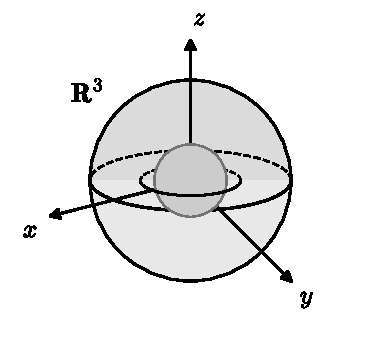
\includegraphics[width=0.72\textwidth]{fig_5.1.pdf}
\caption*{图 5.1\quad 对 $\mathbf{R}^3$（除去原点）用二维球面作叶状分层。}
\end{figure}

让我们考虑几个例子，把讨论拉回地面。最简单的例子是平直的三维欧几里得空间。如果我们选定一个原点，那么 $\mathbf{R}^3$ 显然在绕这个原点的转动下是球对称的。在这样的转动下（也就是说，在 Killing 矢量场的流作用下），点与点相互换位，但每个点都停留在与原点距离固定的一张 $S^2$ 上。

% ---- 书页 199 / p214 ----
这些球面把 $\mathbf{R}^3$ 叶状分层，如图 5.1 所示。当然，它们并没有真正分层整个空间，因为原点自身在转动下原地不动——它不会在某个二维球面上四处移动。但应当清楚，几乎整个空间都被恰当地分层了，而这对我们来说将已经足够。

\begin{figure}[H]
\centering
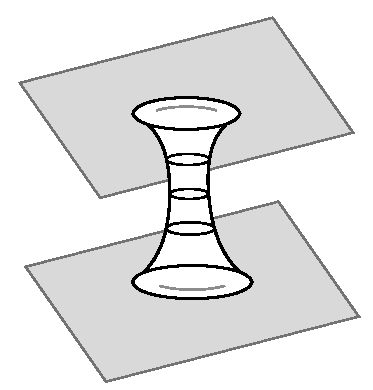
\includegraphics[width=0.72\textwidth]{fig_5.2.pdf}
\caption*{图 5.2\quad 用二维球面对虫洞作叶状分层。}
\end{figure}

我们也可以拥有无需一个原点来绕之转动的球对称性。一个例子是虫洞（wormhole），其拓扑为 $\mathbf{R} \times S^2$。如果我们压掉一个维度，把二维球面画成圆圈，这样的空间看起来可能就像图 5.2 那样。在这个情形下，整个流形都可以被二维球面叶状分层。

既然具有 SO(3) 对称性的流形可以被球面分层，我们的第二步就是要证明 $M$ 上的度规可以化成 (5.24) 的形式。所有球面组成的集合构成一个二维空间（因为四维时空正在被二维球面所分层）。你可能希望我们干脆在每张球面上放坐标 $(\theta, \phi)$，再在所有球面组成的集合上放坐标 $(a, b)$，从而得到 $M$ 上的完整坐标组 $(a, b, \theta, \phi)$。这样一来，每张球面就由 $a = $ 常数、$b = $ 常数确定。我们知道圆球面上的度规是 $\mathrm{d}\Omega^2$，所以这一策略足以保证：把度规限制在任何固定值 $a = a_0$ 和 $b = b_0$（从而 $\mathrm{d}a = \mathrm{d}b = 0$）上时，它取如下形式
\begin{equation*}
\mathrm{d}s^2(a_0, b_0, \theta, \phi) = f(a_0, b_0)\,\mathrm{d}\Omega^2.
\tag{5.27}
\end{equation*}
特别地，函数 $f$ 必须与 $\theta$ 和 $\phi$ 无关，否则球面就会坑坑洼洼而不是圆的。此外，同样清楚的是，把度规限制在任何固定值 $\theta = \theta_0$ 和 $\phi = \phi_0$（从而 $\mathrm{d}\theta = \mathrm{d}\phi = 0$）上时，它取如下形式
\begin{equation*}
\mathrm{d}s^2(a, b, \theta_0, \phi_0) = \mathrm{d}\tau^2(a, b).
\tag{5.28}
\end{equation*}
同样，任何对 $\theta$ 或 $\phi$ 的依赖都会破坏对称性；那将意味着球面之间的横向几何依赖于你处在球面的哪个位置。

然而，我们这样随手铺下这些坐标未免太过草率，因为我们无法排除 $\mathrm{d}a\,\mathrm{d}\theta + \mathrm{d}\theta\,\mathrm{d}a$ 之类的交叉项。换句话说，我们必须小心地把各张球面恰当地对齐，使得沿一条垂直于某张球面的曲线行进时，我们始终保持在常数 $\theta$ 和 $\phi$ 上。为了保证这一点，我们需要更细心地搭建坐标系。先考虑落在某张球面 $S_q$ 上的单个点 $q$（注意 $q$ 不得是所有 Killing 矢量都为零的退化点）。只在这张特定的球面上放坐标 $(\theta, \phi)$，暂不贯穿整个流形。在 $S_q$ 上的每一点 $p$ 处，都会有一个二维正交子空间 $O_p$，它由从 $p$ 出发的那些测地线上的点组成，这些测地线在 $p$ 处的切矢量与 $S_q$ 正交。注意，会存在一个使 $p$ 保持不动的一维转动子群 $R_p$；的确，这些转动把 $p$ 处任何垂直于 $S_q$ 的方向都保持固定，因而整张二维曲面 $O_p$ 在 $R_p$ 下不变。

考虑一个不在 $S_q$ 上、而在分层中某张其他球面 $S_r$ 上的点 $r$，它落在 $p$ 处与 $S_q$ 正交的二维曲面 $O_p$ 内。由于 $p$ 是任意的，这包括了 $S_q$ 邻域内任何可能的点 $r$。注意，$O_p$ 不仅与 $S_q$ 正交，也将与 $S_r$ 正交。为了看清这一点，考虑

% ---- 书页 200 / p215 ----
切空间 $T_rM$ 中与二维曲面 $O_p$ 正交的矢量所构成的二维平面 $V_r$。由于 $O_p$ 在转动 $R_p$ 下不变，而这些转动是等距变换、因而保持正交性，它们必定把 $V_r$ 映到其自身。但 $R_p$ 也把切于 $S_q$ 的矢量集合映到其自身，因为这些转动使各球面保持不变。在四维空间中，同一个点处与给定平面都正交的两个平面必定是同一个平面；因此，切于 $S_r$ 的矢量必定与 $O_p$ 正交。

会有一条唯一的测地线，它与 $S_q$ 正交，并把 $p$ 连到 $r$。沿着这类测地线行进提供了一个映射 $f : S_q \to S_r$，它既是单射又是满射（至少在原先球面的一个邻域内）。我们用这个映射来定义 $S_r$ 上的坐标（类似地也定义任何其他球面上的坐标）：把 $r \in S_r$ 的 $(\theta, \phi)$ 取值指派为点 $p \in S_q$ 处的坐标值。这样我们就在整个流形上定义了 $(\theta, \phi)$。现在为了定义坐标 $(a, b)$，在 $T_qM$ 中生成正交空间 $O_q$ 的那个子空间里选取两个基矢 $S$、$T$。任何其他球面都会由一条唯一的正交测地线与 $q$ 相连，其切矢量为 $aS + bT \in T_qM$。把这些分量 $(a, b)$ 作为该球面上各处的坐标。这就定义了整个流形上的完整坐标组 $(a, b, \theta, \phi)$。

这组坐标下的度规满足 (5.27) 和 (5.28)；尚待证明的是，沿球面的方向与横向方向之间不存在交叉项。这意味着，比方说，矢量场 $\partial_a$ 应当与 $\partial_\theta$ 正交，等等；直接验证可知确实如此。首先，考虑某点 $r \in S_r$ 处的 $\partial_\theta$；这个矢量是沿形如 $x^\mu(\theta) = (a_r, b_r, \theta, \phi_r)$ 的曲线的方向导数。由于 $a$ 和 $b$ 沿曲线为常数，整条曲线都停留在球面 $S_r$ 内，所以 $\partial_\theta$ 切于球面。与此同时，$\partial_a$ 是沿 $x^\mu(a) = (a, b_r, \theta_r, \phi_r)$ 的导数。由于这条曲线停留在正交子空间 $O_r$ 内，$\partial_a$ 将与 $S_r$ 正交，从而与 $\partial_\theta$ 正交。类似的论证保证 $(a, b)$ 与 $(\theta, \phi)$ 之间不存在交叉项。

于是我们已成功地把球对称时空的度规写成如下形式
\begin{equation*}
\mathrm{d}s^2 = g_{aa}(a, b)\,\mathrm{d}a^2 + g_{ab}(a, b)(\mathrm{d}a\,\mathrm{d}b + \mathrm{d}b\,\mathrm{d}a) + g_{bb}(a, b)\,\mathrm{d}b^2 + r^2(a, b)\,\mathrm{d}\Omega^2.
\tag{5.29}
\end{equation*}
这里的 $r(a, b)$ 是某个尚未确定的函数，我们只是给了它一个容易引起联想的标签。不过，没有什么能阻止我们把坐标从 $(a, b)$ 换成 $(a, r)$——只需反解 $r(a, b)$ 即可——除非 $r$ 只是 $a$ 单个变量的函数；在那种情况下，我们照样可以轻而易举地换成 $(b, r)$，所以我们不把这个情形单独考虑。于是度规为
\begin{equation*}
\mathrm{d}s^2 = g_{aa}(a, r)\,\mathrm{d}a^2 + g_{ar}(a, r)(\mathrm{d}a\,\mathrm{d}r + \mathrm{d}r\,\mathrm{d}a) + g_{rr}(a, r)\,\mathrm{d}r^2 + r^2\,\mathrm{d}\Omega^2.
\tag{5.30}
\end{equation*}
我们的下一步是寻找一个函数 $t(a, r)$，使得在 $(t, r)$ 坐标系中度规里不存在交叉项 $\mathrm{d}t\,\mathrm{d}r + \mathrm{d}r\,\mathrm{d}t$。注意到
\begin{equation*}
\mathrm{d}t = \frac{\partial t}{\partial a}\,\mathrm{d}a + \frac{\partial t}{\partial r}\,\mathrm{d}r,
\tag{5.31}
\end{equation*}

% ---- 书页 201 / p216 ----
因此
\begin{equation*}
\mathrm{d}t^2 = \left(\frac{\partial t}{\partial a}\right)^{2}\mathrm{d}a^2 + \left(\frac{\partial t}{\partial a}\right)\left(\frac{\partial t}{\partial r}\right)(\mathrm{d}a\,\mathrm{d}r + \mathrm{d}r\,\mathrm{d}a) + \left(\frac{\partial t}{\partial r}\right)^{2}\mathrm{d}r^2.
\tag{5.32}
\end{equation*}
我们想把度规 (5.30) 中的前三项换成
\begin{equation*}
m\,\mathrm{d}t^2 + n\,\mathrm{d}r^2,
\tag{5.33}
\end{equation*}
其中 $m$、$n$ 是某两个函数。这等价于如下要求：
\begin{equation*}
m\left(\frac{\partial t}{\partial a}\right)^{2} = g_{aa},
\tag{5.34}
\end{equation*}
\begin{equation*}
n + m\left(\frac{\partial t}{\partial r}\right)^{2} = g_{rr},
\tag{5.35}
\end{equation*}
以及
\begin{equation*}
m\left(\frac{\partial t}{\partial a}\right)\left(\frac{\partial t}{\partial r}\right) = g_{ar}.
\tag{5.36}
\end{equation*}
于是我们有三个方程、三个未知量 $t(a, r)$、$m(a, r)$ 和 $n(a, r)$，恰好足以（除 $t$ 的初始条件不计外）把它们完全确定。（当然，这里的“确定”是通过未知函数 $g_{aa}$、$g_{ar}$ 和 $g_{rr}$ 表述的，所以在这个意义上它们其实仍未确定。）这样我们就能把度规写成
\begin{equation*}
\mathrm{d}s^2 = m(t, r)\,\mathrm{d}t^2 + n(t, r)\,\mathrm{d}r^2 + r^2\,\mathrm{d}\Omega^2.
\tag{5.37}
\end{equation*}

到此为止，坐标 $t$ 和 $r$ 之间唯一的差别在于，我们选了 $r$ 作为乘在二维球面度规上的那一个。这样选择的动机来自我们对平直 Minkowski 空间度规的了解，它可以写成 $\mathrm{d}s^2 = -\mathrm{d}t^2 + \mathrm{d}r^2 + r^2\,\mathrm{d}\Omega^2$。我们知道所考虑的时空是洛伦兹型的，所以 $m$ 或 $n$ 中必有一个取负值。让我们选 $\mathrm{d}t^2$ 的系数 $m$ 为负。这并不是一个我们可以随随便便就作出的选择，事实上后面会看到它可能出问题；但我们暂时先这样假定。这个假定并非毫无道理，因为我们知道 Minkowski 空间本身就是球对称的，因而将由 (5.37) 来描述。作了这个选择之后，我们就可以用新的函数 $\alpha$ 和 $\beta$ 来替换函数 $m$ 和 $n$，使得
\begin{equation*}
\mathrm{d}s^2 = -e^{2\alpha(t, r)}\mathrm{d}t^2 + e^{2\beta(t, r)}\mathrm{d}r^2 + r^2\,\mathrm{d}\Omega^2.
\tag{5.38}
\end{equation*}

单靠几何我们最多只能做到这里；关于函数 $\alpha(t, r)$ 和 $\beta(t, r)$，球对称性肯定还不足以说出任何实质性的内容。因此我们的下一步是真正去解 Einstein 方程；步骤与
% ---- 书页 202 / p217 ----
5.1 节中的如出一辙——在那一节里，我们考虑过一个与 (5.38) 类似、但额外假定了时间无关性的度规。这里我们将看到，那个假定其实并不必要，因为解必然是静态的。

(5.38) 的非零 Christoffel 符号为
\begin{equation*}
\begin{array}{lll}
\Gamma^t_{tt} = \partial_t\alpha & \Gamma^t_{tr} = \partial_r\alpha & \Gamma^t_{rr} = e^{2(\beta-\alpha)}\partial_t\beta\\[8pt]
\Gamma^r_{tt} = e^{2(\alpha-\beta)}\partial_r\alpha & \Gamma^r_{tr} = \partial_t\beta & \Gamma^r_{rr} = \partial_r\beta\\[8pt]
\Gamma^\theta_{r\theta} = \dfrac{1}{r} & \Gamma^r_{\theta\theta} = -re^{-2\beta} & \Gamma^\phi_{r\phi} = \dfrac{1}{r}\\[8pt]
\Gamma^r_{\phi\phi} = -re^{-2\beta}\sin^2\theta & \Gamma^\theta_{\phi\phi} = -\sin\theta\cos\theta & \Gamma^\phi_{\theta\phi} = \dfrac{\cos\theta}{\sin\theta},
\end{array}
\tag{5.39}
\end{equation*}
Riemann 张量的非零分量为
\begin{align*}
R^t{}_{rtr} &= e^{2(\beta-\alpha)}\left[\partial_t^2\beta + (\partial_t\beta)^2 - \partial_t\alpha\,\partial_t\beta\right] + \left[\partial_r\alpha\,\partial_r\beta - \partial_r^2\alpha - (\partial_r\alpha)^2\right]\\
R^t{}_{\theta t\theta} &= -re^{-2\beta}\partial_r\alpha\\
R^t{}_{\phi t\phi} &= -re^{-2\beta}\sin^2\theta\,\partial_r\alpha\\
R^t{}_{\theta r\theta} &= -re^{-2\alpha}\partial_t\beta\\
R^t{}_{\phi r\phi} &= -re^{-2\alpha}\sin^2\theta\,\partial_t\beta\\
R^r{}_{\theta r\theta} &= re^{-2\beta}\partial_r\beta\\
R^r{}_{\phi r\phi} &= re^{-2\beta}\sin^2\theta\,\partial_r\beta\\
R^\theta{}_{\phi\theta\phi} &= (1 - e^{-2\beta})\sin^2\theta,
\tag{5.40}
\end{align*}
而 Ricci 张量为
\begin{align*}
R_{tt} &= \left[\partial_t^2\beta + (\partial_t\beta)^2 - \partial_t\alpha\,\partial_t\beta\right] + e^{2(\alpha-\beta)}\left[\partial_r^2\alpha + (\partial_r\alpha)^2 - \partial_r\alpha\,\partial_r\beta + \frac{2}{r}\partial_r\alpha\right]\\
R_{rr} &= -\left[\partial_r^2\alpha + (\partial_r\alpha)^2 - \partial_r\alpha\,\partial_r\beta - \frac{2}{r}\partial_r\beta\right]\\
&\quad + e^{2(\beta-\alpha)}\left[\partial_t^2\beta + (\partial_t\beta)^2 - \partial_t\alpha\,\partial_t\beta\right]\\
R_{tr} &= \frac{2}{r}\partial_t\beta\\
R_{\theta\theta} &= e^{-2\beta}\left[r(\partial_r\beta - \partial_r\alpha) - 1\right] + 1\\
R_{\phi\phi} &= R_{\theta\theta}\sin^2\theta.
\tag{5.41}
\end{align*}
我们的任务是求解真空中的 Einstein 方程 $R_{\mu\nu} = 0$。由 $R_{tr} = 0$ 得到
\begin{equation*}
\partial_t\beta = 0.
\tag{5.42}
\end{equation*}

% ---- 书页 203 / p218 ----
如果我们考虑对 $R_{\theta\theta} = 0$ 取时间导数，并利用 $\partial_t\beta = 0$，就得到
\begin{equation*}
\partial_t\partial_r\alpha = 0.
\tag{5.43}
\end{equation*}
因此可以写出
\begin{align*}
\beta &= \beta(r)\\
\alpha &= f(r) + g(t).
\tag{5.44}
\end{align*}
于是度规 (5.38) 的第一项就是 $-e^{2f(r)}e^{2g(t)}\mathrm{d}t^2$。但我们总可以通过替换 $\mathrm{d}t \to e^{-g(t)}\mathrm{d}t$ 来简单地重新定义时间坐标；换句话说，我们可以自由地选取 $t$ 使 $g(t) = 0$，从而 $\alpha(t, r) = f(r)$。于是我们有
\begin{equation*}
\mathrm{d}s^2 = -e^{2\alpha(r)}\mathrm{d}t^2 + e^{2\beta(r)}\mathrm{d}r^2 + r^2\,\mathrm{d}\Omega^2.
\tag{5.45}
\end{equation*}
度规的所有分量都与坐标 $t$ 无关。因此我们证明了一个至关重要的结果：\emph{任何球对称真空度规都拥有一个类时 Killing 矢量}。

这条性质有趣到配得上一个专属名称：拥有一个在无限远处附近类时的 Killing 矢量的度规称为\textbf{稳态}（stationary）度规。（通常——包括 Schwarzschild 情形在内——在无限远处类时的 Killing 矢量会在内部的某处变成类空的。）在稳态度规中，我们可以选取坐标 $(t, x^1, x^2, x^3)$，使得 Killing 矢量为 $\partial_t$，而且度规分量与 $t$ 无关；稳态度规在这组坐标下的一般形式便为
\begin{equation*}
\mathrm{d}s^2 = g_{00}(\vec{x})\,\mathrm{d}t^2 + g_{0i}(\vec{x})(\mathrm{d}t\,\mathrm{d}x^i + \mathrm{d}x^i\,\mathrm{d}t) + g_{ij}(\vec{x})\,\mathrm{d}x^i\mathrm{d}x^j.
\tag{5.46}
\end{equation*}
还有一个限制更强的性质：如果一个度规拥有一个与某族超曲面正交的类时 Killing 矢量，就称它为\textbf{静态}（static）度规。（关于超曲面的更多细节，见附录 D。）在第 4 章的习题中你证明过，超曲面正交的矢量场 $v^\mu$ 满足
\begin{equation*}
v_{[\mu}\nabla_\nu v_{\rho]} = 0.
\tag{5.47}
\end{equation*}
但有一个更简单的判据：如果我们已经适配好坐标，使分量 $g_{\mu\nu}$ 都与 $t$ 无关，那么 Killing 矢量将与之正交的那些曲面就由条件 $t = $ 常数来定义。在操作层面上，这意味着 (5.46) 中的时间-空间交叉项将不复出现；一般的静态度规可以写成
\begin{equation*}
\mathrm{d}s^2 = g_{00}(\vec{x})\,\mathrm{d}t^2 + g_{ij}(\vec{x})\,\mathrm{d}x^i\mathrm{d}x^j.
\tag{5.48}
\end{equation*}
我们注意到，这种形式中只出现时间坐标 $t$ 的偶数次幂；因此，“静态”的另一种定义是“稳态，且在时间反演 $(t \to -t)$ 下不变”。度规 (5.45) 显然是静态的。你可以把稳态理解为“在每个时刻都精确地做着同一件事情”，而静态则是“根本什么也不做”。

% ---- 书页 204 / p219 ----
例如，静态球对称度规 (5.45) 将描述不旋转的恒星或黑洞，而始终以同样方式旋转的转动系统则将由稳态但非静态的度规来描述。

注意到 (5.45) 恰恰就是 (5.11)——我们在 5.1 节中最初用来导出 Schwarzschild 解的那个度规。因此我们已经证明了 Birkhoff 定理：唯一的球对称真空解就是 Schwarzschild 度规，
\begin{equation*}
\mathrm{d}s^2 = -\left(1 - \frac{2GM}{r}\right)\mathrm{d}t^2 + \left(1 - \frac{2GM}{r}\right)^{-1}\mathrm{d}r^2 + r^2\,\mathrm{d}\Omega^2,
\tag{5.49}
\end{equation*}
一如所允诺的。

对于 Schwarzschild 度规的源，除了要求它球对称之外，我们没有说过任何别的话。具体地说，我们并没有要求源本身是静态的；它完全可以是一颗正在坍缩的恒星，只要坍缩是对称的。因此，像超新星爆发这样的过程，如果它接近球对称，就只会产生非常少的引力辐射（与其他渠道释放的能量相比）——而一颗真实的超新星是否接近球对称，取决于它的起源。这与我们在电磁学中会得到的结果相同：围绕球状电荷分布的电磁场并不依赖于电荷的径向分布。

\section{奇点}

在探究 Schwarzschild 几何中检验粒子的行为之前，我们应该先谈谈奇点（singularity）。从 (5.1) 的形式看，度规系数在 $r = 0$ 和 $r = 2GM$ 处变为无穷——表面上这表明有什么东西出了问题。当然，度规系数是依赖于坐标的量，因此我们不应过分看重它们的数值；完全可能存在坐标奇点（coordinate singularity），它源于某个具体坐标系的失效，而不是底层流形的问题。一个例子出现在平面上极坐标的原点：在那里，度规 $\mathrm{d}s^2 = \mathrm{d}r^2 + r^2\mathrm{d}\theta^2$ 退化，逆度规的分量 $g^{\theta\theta} = r^{-2}$ 发散，尽管流形上的这个点与其他任何点并无不同。

当几何的某处行将失控时，我们应当寻找什么样的坐标无关信号来发出警告呢？事实证明这是一个难以回答的问题，关于广义相对论中奇点的本性，已经有整本整本的著作专门论述。我们不打算深入这个问题，而是转向一个简单的判据来判断何处出了问题——那就是曲率变为无穷大。曲率由 Riemann 张量来量度，但很难说一个张量何时变为无穷，因为它的分量是依赖于坐标的。不过，我们可以由曲率构造出各种标量，而标量是坐标无关的，所以说它们变为无穷是有意义的。最简单的这类标量是 Ricci 标量曲率 $R = g^{\mu\nu}R_{\mu\nu}$，
% 本块末句在原书书页204底部中断（"...the simplest such scalar is the Ricci scalar R = g R," 续接书页205顶部 "but we can also..."）；排版时已将 $R=g^{\mu\nu}R_{\mu\nu}$，随本句放在本块末，避免下一块以数学式开头。下一块请用 %JOIN% 续接本句。
但我们还可以构造更高阶的标量，例如 $R^{\mu\nu}R_{\mu\nu}$、$R^{\mu\nu\rho\sigma}R_{\mu\nu\rho\sigma}$、$R_{\mu\nu\rho\sigma}R^{\rho\sigma\lambda\tau}R_{\lambda\tau}{}^{\mu\nu}$，等等。当我们逼近某个点时，如果这些标量中有任何一个（不必是全部）趋于无穷，我们就把这个点看作曲率的一个奇点。我们还应当检查这个点并不是位于无穷远处；也就是说，沿一条曲线走过有限的距离就能到达它。
% ---- 书页 205 / p220 ----（本页第一段已在上面 tail 中接续，正文自第二段起）
于是，我们有了把一个点当作奇点来对待的充分条件。然而这并不是必要条件，而且一般说来，要证明一个给定的点是非奇异的反而更难；就我们的目的而言，我们只是简单地检验测地线在所讨论的点处是否表现良好，如果表现良好，我们就认为这个点是非奇异的。对于 Schwarzschild 度规 (5.1)，直接计算给出
\begin{equation*}
R^{\mu\nu\rho\sigma}R_{\mu\nu\rho\sigma} = \frac{48G^2M^2}{r^6}.
\tag{5.50}
\end{equation*}
这足以让我们相信，$r = 0$ 代表一个名副其实的奇点。

另一个麻烦之处是 $r = 2GM$，即 Schwarzschild 半径。你可以验证，在那里没有任何曲率不变量发散。于是我们开始倾向于认为它实际上并不奇异，只不过我们选择了一个糟糕的坐标系。最好的办法是，只要可能，就变换到更合适的坐标。我们很快就会看到，在这个例子中这确实是可能的，而且 $r = 2GM$ 这个面在 Schwarzschild 度规中行为良好（尽管很有意思）——它标示出一个黑洞的事件视界（event horizon）。

在为奇点操了一点心之后，我们应当指出，Schwarzschild 半径以内 Schwarzschild 度规的行为对日常生活几乎没有什么影响。我们导出的解只在真空中有效，而且我们预期它在一个球状天体（比如恒星）之外成立。然而，就太阳而言，我们所处理的天体延伸到的半径为
\begin{equation*}
R_\odot = 10^6 GM_\odot.
\tag{5.51}
\end{equation*}
因此，$r = 2GM_\odot$ 深深处于太阳内部，在那里我们并不期望 Schwarzschild 度规适用。实际上，现实的恒星内部解就是把外部的 Schwarzschild 度规与一个在原点处完全光滑的内部度规匹配起来的构造。尽管如此，还是有一些天体需要完整的 Schwarzschild 度规——黑洞——因此在本书的这一章中，我们将让我们的想象力漫游到太阳系之外很远处。

\section{Schwarzschild 测地线}

为了更充分地理解 Schwarzschild 度规，我们将迈出的第一步是考察测地线的行为。我们需要 Schwarzschild 度规的非零 Christoffel 符号：
\begin{equation*}
\begin{array}{lll}
\Gamma^r_{tt} = \dfrac{GM}{r^3}(r-2GM) & \Gamma^r_{rr} = \dfrac{-GM}{r(r-2GM)} & \Gamma^t_{tr} = \dfrac{GM}{r(r-2GM)}\\[10pt]
\Gamma^\theta_{r\theta} = \dfrac{1}{r} & \Gamma^r_{\theta\theta} = -(r-2GM) & \Gamma^\phi_{r\phi} = \dfrac{1}{r}\\[10pt]
\Gamma^r_{\phi\phi} = -(r-2GM)\sin^2\theta & \Gamma^\theta_{\phi\phi} = -\sin\theta\cos\theta & \Gamma^\phi_{\theta\phi} = \dfrac{\cos\theta}{\sin\theta}.
\end{array}
\tag{5.52}
\end{equation*}
于是，测地线方程就变成了以下四个方程，其中 $\lambda$ 是仿射参量：
\begin{gather*}
\frac{\mathrm{d}^2 t}{\mathrm{d}\lambda^2} + \frac{2GM}{r(r-2GM)}\frac{\mathrm{d}r}{\mathrm{d}\lambda}\frac{\mathrm{d}t}{\mathrm{d}\lambda} = 0,\\[8pt]
\frac{\mathrm{d}^2 r}{\mathrm{d}\lambda^2} + \frac{GM}{r^3}(r-2GM)\left(\frac{\mathrm{d}t}{\mathrm{d}\lambda}\right)^2 - \frac{GM}{r(r-2GM)}\left(\frac{\mathrm{d}r}{\mathrm{d}\lambda}\right)^2\\[2pt]
-\,(r-2GM)\left[\left(\frac{\mathrm{d}\theta}{\mathrm{d}\lambda}\right)^2 + \sin^2\theta\left(\frac{\mathrm{d}\phi}{\mathrm{d}\lambda}\right)^2\right] = 0,\\[8pt]
\frac{\mathrm{d}^2\theta}{\mathrm{d}\lambda^2} + \frac{2}{r}\frac{\mathrm{d}\theta}{\mathrm{d}\lambda}\frac{\mathrm{d}r}{\mathrm{d}\lambda} - \sin\theta\cos\theta\left(\frac{\mathrm{d}\phi}{\mathrm{d}\lambda}\right)^2 = 0,\\[8pt]
\frac{\mathrm{d}^2\phi}{\mathrm{d}\lambda^2} + \frac{2}{r}\frac{\mathrm{d}\phi}{\mathrm{d}\lambda}\frac{\mathrm{d}r}{\mathrm{d}\lambda} + 2\frac{\cos\theta}{\sin\theta}\frac{\mathrm{d}\theta}{\mathrm{d}\lambda}\frac{\mathrm{d}\phi}{\mathrm{d}\lambda} = 0.
\tag{5.53}
\end{gather*}
指望一眼看出这组耦合方程的解来，希望似乎不大。幸运的是，Schwarzschild 度规的高度对称性使我们的任务大为简化。我们知道有四个 Killing 矢量：三个对应球对称性，一个对应时间平移。其中每一个都会给出自由粒子的一个运动常数（constant of the motion）。如果 $K^\mu$ 是一个 Killing 矢量，我们知道
\begin{equation*}
K_\mu\frac{\mathrm{d}x^\mu}{\mathrm{d}\lambda} = \mathrm{constant}.
\tag{5.54}
\end{equation*}
此外，对测地线我们总是还有另一个运动常数：测地线方程（连同度规相容性）意味着如下这个量
\begin{equation*}
\epsilon = -g_{\mu\nu}\frac{\mathrm{d}x^\mu}{\mathrm{d}\lambda}\frac{\mathrm{d}x^\nu}{\mathrm{d}\lambda}
\tag{5.55}
\end{equation*}
沿路径是常数。（对任何一条轨迹，我们都可以选取参量 $\lambda$ 使得 $\epsilon$ 为常数；我们只是指出，这与沿测地线的仿射参数化是相容的。）当然，对有质量粒子我们通常取 $\lambda = \tau$，这个关系就简单地变成 $\epsilon = -g_{\mu\nu}U^\mu U^\nu = +1$。而对沿类光轨迹运动的无质量粒子，我们总有 $\epsilon = 0$，

% ---- 书页 207 / p222 ----
而这个方程并不固定参量 $\lambda$。正如 3.4 节所讨论的，方便的做法是在类光测地线上把 $\lambda$ 归一化，使得四维动量与四速度相等，$p^\mu = \mathrm{d}x^\mu/\mathrm{d}\lambda$。我们也可能关心类空测地线（尽管它们并不对应粒子的路径），对它们我们将取 $\epsilon = -1$。

我们并不急于立刻写出与 Killing 矢量相联系的四个守恒量的显式表达式，而是先想一想它们在告诉我们什么。注意，它们所代表的对称性在平直时空中也同样存在，而在那里它们导致的守恒量是我们非常熟悉的。时间平移下的不变性导致能量守恒，而空间转动下的不变性导致角动量三个分量的守恒。本质上相同的事情也适用于 Schwarzschild 度规。我们可以把角动量想成一个三矢量，它具有一个大小（一个分量）和一个方向（两个分量）。角动量方向的守恒意味着粒子将在一个平面内运动。我们可以选取这个平面为坐标系的赤道面；如果粒子不在这个平面内，我们可以转动坐标，直到它在平面内为止。于是，导致角动量方向守恒的那两个 Killing 矢量就意味着，对一个单独的粒子，我们可以选取
\begin{equation*}
\theta = \frac{\pi}{2}.
\tag{5.56}
\end{equation*}
剩下的两个 Killing 矢量分别对应能量和角动量的大小。能量来自类时 Killing 矢量
\begin{equation*}
K^\mu = (\partial_t)^\mu = (1, 0, 0, 0).
\tag{5.57}
\end{equation*}
以角动量的大小为守恒量的那个 Killing 矢量则是
\begin{equation*}
R^\mu = (\partial_\phi)^\mu = (0, 0, 0, 1).
\tag{5.58}
\end{equation*}
在这两种情形下，方便的做法都是降指标，得到
\begin{equation*}
K_\mu = \left(-\left(1-\frac{2GM}{r}\right), 0, 0, 0\right)
\tag{5.59}
\end{equation*}
以及
\begin{equation*}
R_\mu = \left(0, 0, 0, r^2\sin^2\theta\right).
\tag{5.60}
\end{equation*}
由于 (5.56) 意味着在我们感兴趣的测地线上 $\sin\theta = 1$，这两个守恒量便是
\begin{equation*}
E = -K_\mu\frac{\mathrm{d}x^\mu}{\mathrm{d}\lambda} = \left(1-\frac{2GM}{r}\right)\frac{\mathrm{d}t}{\mathrm{d}\lambda}
\tag{5.61}
\end{equation*}

% ---- 书页 208 / p223 ----
以及
\begin{equation*}
L = R_\mu\frac{\mathrm{d}x^\mu}{\mathrm{d}\lambda} = r^2\frac{\mathrm{d}\phi}{\mathrm{d}\lambda}.
\tag{5.62}
\end{equation*}
对无质量粒子，这些量可以认为是守恒的能量和角动量；而对有质量粒子，它们是粒子单位质量的守恒能量和角动量。在下一章讨论转动黑洞时，我们将用 $E$ 和 $L$ 指真实的能量和角动量，而不是“每单位质量”的量；其含义从上下文应该看得很清楚。注意，(5.62) 的守恒性正是 Kepler 第二定律在广义相对论中的对应物——相等的时间里扫出相等的面积。

回忆一下，在 3.4 节中我们曾断言，一个四维动量为 $p^\mu$ 的粒子的能量，由具有四速度 $U^\mu$ 的观者测量，应为 $-p_\mu U^\mu$。这个量并\emph{不}等于 (5.61)，甚至不与它成正比，即使把观者取为稳态的（$U^i = 0$）也是如此。从数学上看，这是因为四速度归一化为 $U_\mu U^\mu = -1$，而 Killing 矢量 $K^\mu$ 却不是这样：如果我们试图那样把它归一化，它就不再求解 Killing 方程了。在稍微深一个层次上，$-p_\mu U^\mu$ 可以认为是粒子的惯性能/动能，而 $-p_\mu K^\mu$ 则是总的守恒能量，其中包含引力场带来的势能。引力势能的概念并不总是良定义的，但只要存在类时 Killing 矢量，总能量就是良定义的。我们马上就会用 $E$ 来帮助刻画 Schwarzschild 的测地线；稍后我们还会把 $-p_\mu U^\mu$ 用于无质量粒子，在那里它可以认为是光子的观测频率，用来描述引力红移。

守恒量 $E$ 和 $L$ 合在一起，为理解 Schwarzschild 几何中粒子的轨道提供了方便的途径。让我们把 (5.55) 的 $\epsilon$ 表达式展开，得到
\begin{equation*}
-\left(1-\frac{2GM}{r}\right)\left(\frac{\mathrm{d}t}{\mathrm{d}\lambda}\right)^2 + \left(1-\frac{2GM}{r}\right)^{-1}\left(\frac{\mathrm{d}r}{\mathrm{d}\lambda}\right)^2 + r^2\left(\frac{\mathrm{d}\phi}{\mathrm{d}\lambda}\right)^2 = -\epsilon.
\tag{5.63}
\end{equation*}
如果我们把它乘以 $(1-2GM/r)$，并用 $E$ 和 $L$ 的表达式，就得到
\begin{equation*}
-E^2 + \left(\frac{\mathrm{d}r}{\mathrm{d}\lambda}\right)^2 + \left(1-\frac{2GM}{r}\right)\left(\frac{L^2}{r^2}+\epsilon\right) = 0.
\tag{5.64}
\end{equation*}
这肯定是进展：我们已经把一个凌乱的耦合方程组变成了关于 $r(\lambda)$ 的单独一个方程。如果我们把它改写成
\begin{equation*}
\frac{1}{2}\left(\frac{\mathrm{d}r}{\mathrm{d}\lambda}\right)^2 + V(r) = \mathcal{E},
\tag{5.65}
\end{equation*}

% ---- 书页 209 / p224 ----
\begin{figure}[H]
\centering
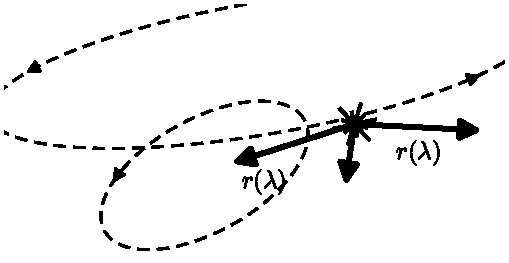
\includegraphics[width=0.72\textwidth]{fig_5.3.pdf}
\caption*{图 5.3\quad 围绕恒星的轨道，由把半径 $r$ 表示为参量 $\lambda$ 的函数来刻画。}
\end{figure}
其中
\begin{equation*}
V(r) = \frac{1}{2}\epsilon - \epsilon\frac{GM}{r} + \frac{L^2}{2r^2} - \frac{GML^2}{r^3}
\tag{5.66}
\end{equation*}
而
\begin{equation*}
\mathcal{E} = \frac{1}{2}E^2.
\tag{5.67}
\end{equation*}
在 (5.65) 中，我们得到的恰恰是一个单位质量的经典粒子在由 $V(r)$ 给出的一维势中、带着“能量”$\mathcal{E}$ 运动时的方程。这有点令人混淆，但还不算太糟：单位质量的守恒能量是 $E$，而坐标 $r$ 的有效势（effective potential）对应的却是 $\mathcal{E} = E^2/2$。

当然，我们的物理处境与在一维中运动的经典粒子相当不同；我们所考虑的轨迹是绕恒星或其他天体的轨道，如图 5.3 所示。我们感兴趣的量不仅有 $r(\lambda)$，还有 $t(\lambda)$ 和 $\phi(\lambda)$。尽管如此，通过理解轨道的径向行为，我们就能朝着理解所有轨道的目标走得非常远，而把这些行为约化成一个我们知道怎样求解的问题，帮助极大。

对 Newton 引力中的轨道做类似的分析也会给出类似的结果；一般方程 (5.65) 将会相同，但有效势 (5.66) 将不会含有最后一项。（注意，这个方程不是 $1/r$ 的幂级数，它是精确的。）在势 (5.66) 中，第一项只是一个常数，第二项恰好对应 Newton 引力势，第三项是来自角动量的贡献，它在 Newton 引力和广义相对论中取相同的形式。最后一项——广义相对论的贡献——将被证明会带来巨大的差别，尤其是在 $r$ 很小的地方。

\begin{figure}[H]
\centering
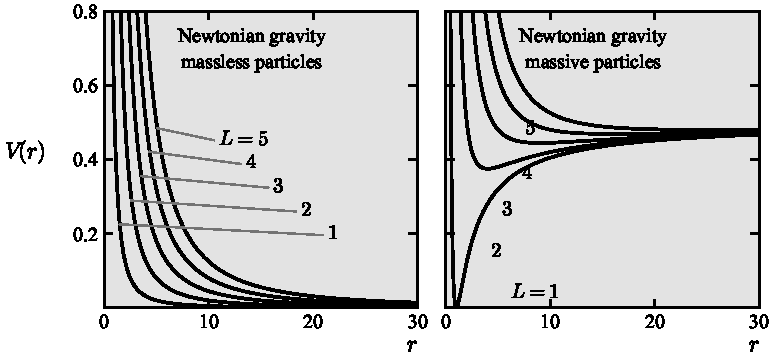
\includegraphics[width=0.72\textwidth]{fig_5.4.pdf}
\caption*{图 5.4\quad Newton 引力中的有效势。图中画出五条曲线，对应所标出的（单位质量的）角动量 $L$ 值，我们取 $GM = 1$。注意，只要能量足够大，每条轨道都会到达一个转折点并返回无穷远。}
\end{figure}
让我们来考察各种可能类型的轨道所对应的有效势，如图 5.4 和图 5.5 所示。不同的 $L$ 值有不同的曲线 $V(r)$；对其中任何一条曲线，轨道的行为都可以通过把 $\mathcal{E}$ 与 $V(r)$ 相比较来判断。粒子的一般行为将是在势中运动，直到它到达 $V(r) = \mathcal{E}$ 的一个“转折点”（turning point），这时它将开始
% ---- 书页 210 / p225 ----
朝另一个方向运动。有时可能没有转折点可碰，这时粒子就一直走下去。另一些情形下，粒子可以干脆在半径 $r_c$ 为常数的圆轨道上运动；这可能发生在势是平坦的地方，即 $\mathrm{d}V/\mathrm{d}r = 0$ 处。对 (5.66) 求微商，我们发现圆轨道出现在
\begin{equation*}
\epsilon GM r_c^2 - L^2 r_c + 3GML^2\gamma = 0,
\tag{5.68}
\end{equation*}
其中在 Newton 引力中 $\gamma = 0$，在广义相对论中 $\gamma = 1$。如果圆轨道对应势的极小值，它将是稳定的；如果对应极大值，则是不稳定的。非圆的束缚轨道将围绕稳定圆轨道的半径振荡。

转向 Newton 引力，我们发现圆轨道出现在
\begin{equation*}
r_c = \frac{L^2}{\epsilon GM}.
\tag{5.69}
\end{equation*}
\begin{figure}[H]
\centering
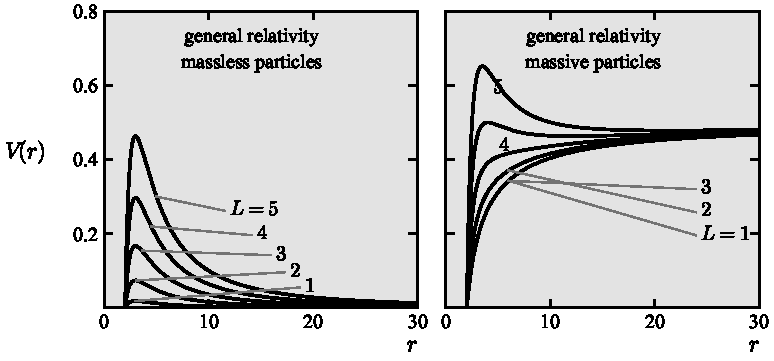
\includegraphics[width=0.72\textwidth]{fig_5.5.pdf}
\caption*{图 5.5\quad 广义相对论中的有效势。同样画出五条曲线，对应所标出的（单位质量的）角动量 $L$ 值，我们取 $GM = 1$。在广义相对论中存在一个大于或等于 $3GM$ 的最内层圆轨道，任何落到这个半径以内的轨道都会一直落到 $r = 0$（对沿测地线运动的粒子而言）。}
\end{figure}
对无质量粒子，$\epsilon = 0$，不存在圆轨道；这与图 5.4 中的第一幅图相一致，该图表明没有任何形式的束缚轨道。尽管在极坐标下这一点有些被掩盖，无质量粒子实际上沿直线运动，因为作用在无质量粒子上的 Newton 引力为零。当然，无质量粒子在 Newton 理论中的地位本来就有些成问题，所以随着你所做假设的不同，你可能得到不同的答案。用有效势的语言来说，一个具有给定能量 $E$ 的光子将从 $r = \infty$ 进入并逐渐减慢（实际上减慢的是 $\mathrm{d}r/\mathrm{d}\lambda$，光速并没有改变），直到它到达
% ---- 书页 211 / p226 ----
转折点，这时它将开始折返，回到 $r = \infty$。较低的 $L$ 值——光子在这些情形下会更靠近一些才开始折返——不过是那些初始瞄准得更贴近引力天体的轨迹。对有质量粒子，在半径 (5.69) 处将有稳定圆轨道，还有围绕这个半径振荡的束缚轨道。如果能量大于渐近值 $E = 1$，轨道将是非束缚的，描述一个先接近恒星然后再退离的粒子。我们知道，Newton 理论中的轨道是圆锥曲线（conic sections）——束缚轨道不是圆就是椭圆，而非束缚轨道不是抛物线就是双曲线——尽管我们不打算在这里证明这一点。

在广义相对论中，情况有所不同，但只在 $r$ 足够小时才如此。既然差别就在于 $-GML^2/r^3$ 这一项，当 $r \to \infty$ 时两种理论中的行为完全相同。但当 $r \to 0$ 时，势趋于 $-\infty$，而不像 Newton 情形那样趋于 $+\infty$。在 $r = 2GM$ 处，势总是零；这个半径以内就是黑洞，我们稍后会更彻底地讨论它。对无质量粒子，总存在一个势垒（除了 $L = 0$ 的情形，此时势恒等于零），但一个能量足够高的光子仍然会越过势垒，被无可挽回地拖向中心。注意，“能量足够高”指的是“与它的角动量相比”——事实上光子的频率无关紧要，要紧的只是它所指向的方向。势垒的顶部是不稳定的圆轨道。对 $\epsilon = 0$、$\gamma = 1$，我们可以很容易地求解 (5.68)，得到
\begin{equation*}
r_c = 3GM.
\tag{5.70}
\end{equation*}

% ---- 书页 212 / p227 ----
图 5.5 的第一幅图证实了这一点：对每个 $L$，$V(r)$ 都在 $r = 3GM$ 处有一个极大值。这意味着光子可以在这个半径的圆上永远运转下去，但任何微扰都会使它飞走，不是飞向 $r = 0$，就是飞向 $r = \infty$。

对有质量粒子，随着角动量的不同，再一次出现不同的区域。圆轨道位于
\begin{equation*}
r_c = \frac{L^2 \pm \sqrt{L^4 - 12G^2M^2L^2}}{2GM}.
\tag{5.71}
\end{equation*}
对大的 $L$，将有两个圆轨道，一个稳定，一个不稳定。在 $L \to \infty$ 的极限下，它们的半径为
\begin{equation*}
r_c = \frac{L^2 \pm L^2(1-6G^2M^2/L^2)}{2GM} = \left(\frac{L^2}{GM},\, 3GM\right).
\tag{5.72}
\end{equation*}
在这个极限下，稳定圆轨道移向更远处，而不稳定圆轨道则趋近 $3GM$，这种行为与无质量情形相类似。当我们减小 $L$ 时，两个圆轨道彼此靠近；当 (5.71) 中的判别式消失时，它们重合，此时
\begin{equation*}
L = \sqrt{12}\,GM,
\tag{5.73}
\end{equation*}
相应地
\begin{equation*}
r_c = 6GM,
\tag{5.74}
\end{equation*}
而对更小的 $L$，它们就完全消失了。因此，$6GM$ 是 Schwarzschild 度规中稳定圆轨道可能具有的最小半径。还有非束缚轨道，它们从无穷远进来然后折返；还有束缚但非圆的轨道，它们围绕稳定圆轨道的半径振荡。注意，这类轨道在 Newton 引力中会描绘出严格的圆锥曲线，在广义相对论中则不会如此，尽管要证明这一点我们还必须求解 $\mathrm{d}\phi/\mathrm{d}\lambda$ 的方程。最后，还有一些轨道从无穷远进来，一直落到 $r = 0$；这既可能发生在能量高于势垒的时候，也可能发生在 $L < \sqrt{12}\,GM$、势垒完全消失的时候。

于是我们发现，Schwarzschild 解在 $r > 6GM$ 拥有稳定圆轨道，在 $3GM < r < 6GM$ 拥有不稳定圆轨道。需要记住的重要一点是，这些仅仅是测地线；没有什么能阻止一个加速的粒子下潜到 $r = 3GM$ 以下再冒出来，只要它保持在 $r = 2GM$ 之外就好。

\section{实验检验}

广义相对论的大多数实验检验都涉及检验粒子在太阳系中的运动，因而是 Schwarzschild 度规的测地线问题。Einstein 曾提出三项检验：
% ---- 书页 213 / p228 ----（书页 213 实际自“Einstein 曾提出”起，注释随整句顺延） ----光线偏折、近日点进动（precession of perihelia）和引力红移。
\begin{figure}[H]
\centering
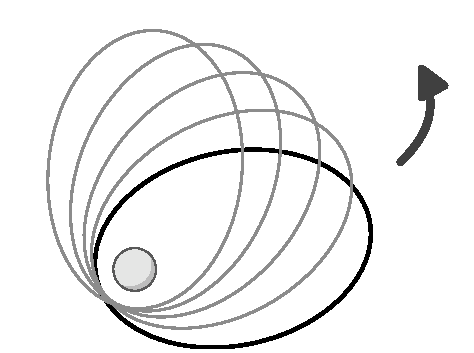
\includegraphics[width=0.72\textwidth]{fig_5.6.pdf}
\caption*{图 5.6\quad 广义相对论中的轨道描绘出进动的椭圆。}
\end{figure}
光线偏折在弱场极限（weak-field limit）下就可以观测，因此放在第 7 章讨论。本节我们将讨论近日点进动和引力红移。（椭圆轨道的近日点（perihelion）是它最接近太阳的那一点；绕地球或恒星的轨道则分别有近地点（perigee）和近星点（periastron）。）

近日点进动反映了这样一个事实：广义相对论中的非圆轨道并不是完美的闭合椭圆；在相当好的近似下，它们是进动着的椭圆，画出如图 5.6 所示的花瓣图案。尽管概念上简单，近日点进动的速率算起来却有些繁琐；这里我们遵循 d'Inverno（1992）的做法。策略是把径向坐标 $r$ 的演化描述为角坐标 $\phi$ 的函数；对一个完美的椭圆，$r(\phi)$ 将以 $2\pi$ 为周期，这反映了近日点在每一圈轨道都出现在相同角位置的事实。利用微扰论，我们可以展示广义相对论如何给周期带来微小的改变，从而产生进动。

我们从 Schwarzschild 度规中有质量粒子的径向运动方程 (5.65) 出发。为了得到 $\mathrm{d}r/\mathrm{d}\phi$ 的方程，我们乘以
\begin{equation*}
\left(\frac{\mathrm{d}\phi}{\mathrm{d}\lambda}\right)^{-2} = \frac{r^4}{L^2},
\tag{5.75}
\end{equation*}
这给出
\begin{equation*}
\left(\frac{\mathrm{d}r}{\mathrm{d}\phi}\right)^2 + \frac{1}{L^2}r^4 - \frac{2GM}{L^2}r^3 + r^2 - 2GMr = \frac{2\mathcal{E}}{L^2}r^4.
\tag{5.76}
\end{equation*}
在求解这个方程时，有两个技巧很有用。第一个技巧是定义一个新变量

% ---- 书页 214 / p229 ----
\begin{equation*}
x = \frac{L^2}{GMr}.
\tag{5.77}
\end{equation*}
由 (5.69) 我们看到，在 Newton 圆轨道处 $x = 1$。我们的运动方程 (5.76) 变为
\begin{equation*}
\left(\frac{\mathrm{d}x}{\mathrm{d}\phi}\right)^2 + \frac{L^2}{G^2M^2} - 2x + x^2 - \frac{2G^2M^2}{L^2}x^3 = \frac{2\mathcal{E}L^2}{G^2M^2}.
\tag{5.78}
\end{equation*}
第二个技巧是把它对 $\phi$ 求微商，得到 $x(\phi)$ 的一个二阶方程：
\begin{equation*}
\frac{\mathrm{d}^2 x}{\mathrm{d}\phi^2} - 1 + x = \frac{3G^2M^2}{L^2}x^2.
\tag{5.79}
\end{equation*}
在 Newton 计算中最后一项将不存在，我们可以精确解出 $x$；在这里，我们可以把它当作微扰来处理。

我们把 $x$ 展开成 Newton 解加上一个小的偏离，
\begin{equation*}
x = x_0 + x_1.
\tag{5.80}
\end{equation*}
(5.79) 的零阶部分便是
\begin{equation*}
\frac{\mathrm{d}^2 x_0}{\mathrm{d}\phi^2} - 1 + x_0 = 0
\tag{5.81}
\end{equation*}
而一阶部分是
\begin{equation*}
\frac{\mathrm{d}^2 x_1}{\mathrm{d}\phi^2} + x_1 = \frac{3G^2M^2}{L^2}x_0^2.
\tag{5.82}
\end{equation*}
零阶方程的解可以写成
\begin{equation*}
x_0 = 1 + e\cos\phi.
\tag{5.83}
\end{equation*}
这是 Newton 或 Kepler 的标准结果；它描述一个完美的椭圆，$e$ 是偏心率（eccentricity）。一个椭圆由半长轴（semi-major axis）$a$——从中心到椭圆上最远点的距离——和半短轴（semi-minor axis）$b$——从中心到最近点的距离——确定。偏心率满足 $e^2 = 1 - b^2/a^2$。

把 Newton 解代入一阶方程 (5.82)，我们得到
\begin{align*}
\frac{\mathrm{d}^2 x_1}{\mathrm{d}\phi^2} + x_1 &= \frac{3G^2M^2}{L^2}(1+e\cos\phi)^2\\
&= \frac{3G^2M^2}{L^2}\left[\left(1+\frac{1}{2}e^2\right) + 2e\cos\phi + \frac{1}{2}e^2\cos 2\phi\right].
\tag{5.84}
\end{align*}

% ---- 书页 215 / p230 ----
为了求解这个方程，注意到
\begin{equation*}
\frac{\mathrm{d}^2}{\mathrm{d}\phi^2}(\phi\sin\phi) + \phi\sin\phi = 2\cos\phi
\tag{5.85}
\end{equation*}
以及
\begin{equation*}
\frac{\mathrm{d}^2}{\mathrm{d}\phi^2}(\cos 2\phi) + \cos 2\phi = -3\cos 2\phi.
\tag{5.86}
\end{equation*}
把它们与 (5.84) 相比较，我们看到一个解由下式给出
\begin{equation*}
x_1 = \frac{3G^2M^2}{L^2}\left[\left(1+\frac{1}{2}e^2\right) + e\phi\sin\phi - \frac{1}{6}e^2\cos 2\phi\right],
\tag{5.87}
\end{equation*}
欢迎大家自行验证。这里的三项性质各不相同：第一项只是一个常数的移动，而第三项则在零附近振荡。重要的效应于是包含在第二项中，它在一圈接一圈的轨道上不断累积。因此我们把这一项与零阶解合并，写成
\begin{equation*}
x = 1 + e\cos\phi + \frac{3G^2M^2e}{L^2}\phi\sin\phi.
\tag{5.88}
\end{equation*}
即使对微扰后的方程来说，这也不是一个完整的解，但它概括了我们关心的部分。特别地，$x$ 的这个表达式可以方便地改写成一个角周期并不完全恰好是 $2\pi$ 的椭圆方程：
\begin{equation*}
x = 1 + e\cos[(1-\alpha)\phi],
\tag{5.89}
\end{equation*}
其中我们引入了
\begin{equation*}
\alpha = \frac{3G^2M^2}{L^2}.
\tag{5.90}
\end{equation*}
(5.88) 与 (5.89) 的等价性，可以通过把 $\cos[(1-\alpha)\phi]$ 按小参量 $\alpha$ 展开成幂级数看出来：
\begin{align*}
\cos[(1-\alpha)\phi] &= \cos\phi + \alpha\frac{\mathrm{d}}{\mathrm{d}\alpha}\cos[(1-\alpha)\phi]_{\alpha=0}\\
&= \cos\phi + \alpha\phi\sin\phi.
\tag{5.91}
\end{align*}

于是我们发现，行星每运转一圈，近日点就前进一个角度
\begin{equation*}
\Delta\phi = 2\pi\alpha = \frac{6\pi G^2M^2}{L^2}.
\tag{5.92}
\end{equation*}
为了把角动量 $L$ 换算成更常用的量，我们可以使用对 Newton 轨道有效的表达式，因为我们所考察的这个量已经是
% ---- 书页 216 / p231 ----
一个小的微扰了。一个普通的椭圆满足
\begin{equation*}
r = \frac{(1-e^2)a}{1+e\cos\phi},
\tag{5.93}
\end{equation*}
其中 $a$ 是半长轴。与我们的零阶解 (5.83) 以及 $x$ 的定义 (5.77) 相比较，我们看到
\begin{equation*}
L^2 \approx GM(1-e^2)a.
\tag{5.94}
\end{equation*}
这是一个近似，在轨道是完美闭合椭圆的前提下成立。把它代入 (5.92)，并恢复光速的显式因子，我们得到
\begin{equation*}
\Delta\phi = \frac{6\pi GM}{c^2(1-e^2)a}.
\tag{5.95}
\end{equation*}
历史上，水星的近日点进动是广义相对论的第一个检验。事实上，早在 Einstein 发明广义相对论之前，人们就已经知道水星轨道存在一个表观上的偏差，并且已经提出了若干种解决方案（包括太阳系内部的“暗物质”）。Einstein 了解这个偏差，他在建立广义相对论之后最初的任务之一，就是证明它正确地解释了水星的近日点进动。对水星绕太阳的运动，相关的轨道参量为
\begin{equation*}
\begin{array}{c}
\dfrac{GM_\odot}{c^2} = 1.48\times 10^5\,\mathrm{cm},\\[8pt]
a = 5.79\times 10^{12}\,\mathrm{cm}\\[6pt]
e = 0.2056,
\end{array}
\tag{5.96}
\end{equation*}
当然还有 $c = 3.00\times 10^{10}\,\mathrm{cm/sec}$。这就给出
\begin{equation*}
\Delta\phi_{\mathrm{Mercury}} = 5.01\times 10^{-7}\,\mathrm{radians/orbit} = 0.103^{\prime\prime}/\mathrm{orbit},
\tag{5.97}
\end{equation*}
其中 $''$ 代表角秒。更常见的做法是用每世纪的进动来表示；水星每 88 天运转一周，由此得到
\begin{equation*}
\Delta\phi_{\mathrm{Mercury}} = 43.0^{\prime\prime}/\mathrm{century}.
\tag{5.98}
\end{equation*}
于是，水星轨道的长轴以每 100 年 43.0 角秒的速率进动。观测值是 5601 角秒/100 年。然而，其中大部分来自我们的地心坐标系中分点的岁差（precession of equinoxes）；精确地说，是 5025 角秒/100 年。其他行星的引力摄动又贡献了额外的 532 角秒/100 年，剩下 43 角秒/100 年有待广义相对论来解释，而它解释得相当好。可以想见，Einstein 第一次算出这个结果时一定非常高兴。

在第 2 章中，我们把光子的引力红移当作等效原理的一个推论讨论过。Schwarzschild 度规是一个精确
% 本块末句在原书书页 216 底部中断（"...The Schwarzschild metric is an exact" 续接书页 217 顶部），下一块需用 %JOIN% 续接本句。
解，因而应当预言一种在时空小区域内退化为等效原理（EP）预言的红移。让我们来看看这是如何实现的。

% ---- 书页 217 / p232 ----
考虑一个四速度为 $U^\mu$、在 Schwarzschild 坐标中静止（$U^i = 0$）的观者。我们本可以允许这个观者运动，但那只不过是在引力效应之上叠加一个通常的多普勒频移而已。四速度满足 $U_\mu U^\mu = -1$，对于 Schwarzschild 时空中的静止观者，这就意味着
\begin{equation*}
U^0 = \left(1 - \frac{2GM}{r}\right)^{-1/2}.
\tag{5.99}
\end{equation*}
任何一个这样的观者，测量沿类光测地线 $x^\mu(\lambda)$ 传播的光子的频率，得到的都是
\begin{equation*}
\omega = -g_{\mu\nu}U^\mu\frac{\mathrm{d}x^\nu}{\mathrm{d}\lambda}.
\tag{5.100}
\end{equation*}
实际上，正是这个关系定义了 $\lambda$ 的归一化。于是我们有
\begin{align*}
\omega &= \left(1 - \frac{2GM}{r}\right)^{1/2}\frac{\mathrm{d}t}{\mathrm{d}\lambda}
\tag{5.101}\\
&= \left(1 - \frac{2GM}{r}\right)^{-1/2}E,
\tag{5.102}
\end{align*}
其中 $E$ 由式 (5.61) 定义，只是应用于光子的轨迹。$E$ 是守恒量，因此在不同的径向距离处测量时，$\omega$ 显然会取不同的值。对于在 $r_1$ 处发射、在 $r_2$ 处被观测到的光子，观测到的频率之间将有如下关系
\begin{equation*}
\frac{\omega_2}{\omega_1} = \left(\frac{1 - 2GM/r_1}{1 - 2GM/r_2}\right)^{1/2}.
\tag{5.103}
\end{equation*}
这是频移的一个精确结果；在 $r \gg 2GM$ 的极限下，我们得到
\begin{align*}
\frac{\omega_2}{\omega_1} &= 1 - \frac{GM}{r_1} + \frac{GM}{r_2}\\
&= 1 + \Phi_1 - \Phi_2,
\tag{5.104}
\end{align*}
其中 $\Phi = -GM/r$ 是 Newton 引力势。这告诉我们，当 $\Phi$ 增大时频率会降低——而这正是我们从引力场中向外爬升时发生的事情：于是就出现了红移。（落向引力体的光子则会发生蓝移。）我们看到，$r \gg 2GM$ 的结果与基于等效原理的计算相一致。

引力红移最早由 Pound 与 Rebka 于 1960 年探测到，他们让 $\gamma$ 射线向上穿行仅仅 72 英尺（哈佛大学物理系大楼的高度）的距离。后来的检验变得越来越精确，往往利用人造飞船或放置在飞机上的原子钟。在所有这些情形中，与 Einstein 预言的符合程度都极为出色。

% ---- 书页 218 / p233 ----
自 Einstein 提出三大经典检验以来，人们又提出了对广义相对论的若干进一步检验。其中最著名的当然是脉冲双星，我们将在第 7 章讨论。另一个是引力时间延迟，由 Shapiro 发现并观测到，同样在第 7 章讨论。在一个非常不同的情境下，大爆炸核合成为广义相对论提供了一个宇宙学检验——它发生在宇宙仅诞生几秒钟的年代，将在第 8 章讨论。现代的进展还引入了大量新的检验；全面的介绍可参阅 Will (1981)。

\section{Schwarzschild 黑洞}

现在，对于麻烦半径 $r = 2GM$ 之外测地线的行为我们已经有所了解——这正是太阳系以及其他大多数天体物理情形所关心的区域。接下来我们转而研究这样一些天体：即使在半径小于 $2GM$ 处，它们仍然由 Schwarzschild 解描述——黑洞。（我们暂时先使用“黑洞”这个术语，尽管还没有为这样一种天体引入确切的含义。）

理解一个时空的几何的办法之一，是考察由光锥定义的因果结构。因此我们考虑径向类光曲线，即 $\theta$ 和 $\phi$ 保持不变且 $\mathrm{d}s^2 = 0$ 的曲线：
\begin{equation*}
\mathrm{d}s^2 = 0 = -\left(1 - \frac{2GM}{r}\right)\mathrm{d}t^2 + \left(1 - \frac{2GM}{r}\right)^{-1}\mathrm{d}r^2,
\tag{5.105}
\end{equation*}
由此我们得到
\begin{equation*}
\frac{\mathrm{d}t}{\mathrm{d}r} = \pm\left(1 - \frac{2GM}{r}\right)^{-1}.
\tag{5.106}
\end{equation*}
当然，这量度的正是 $t$-$r$ 平面的时空图上光锥的斜率。$r$ 很大时斜率为 $\pm 1$，与平直空间中一样；而当我们接近 $r = 2GM$ 时，$\mathrm{d}t/\mathrm{d}r \to \pm\infty$，光锥便“闭合”起来，如图 5.7 所示。因此，接近 $r = 2GM$ 的光线似乎永远到不了那里——至少在这个坐标系中是如此；它看起来是渐近地趋于这个半径。

\begin{figure}[H]
\centering
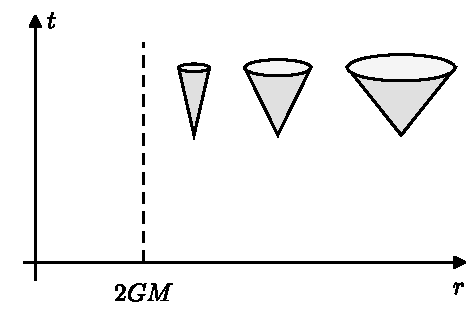
\includegraphics[width=0.72\textwidth]{fig_5.7.pdf}
\caption*{图 5.7\quad 在 Schwarzschild 坐标中，当我们接近 $r = 2GM$ 时，光锥看似逐渐闭合。}
\end{figure}
正如我们将要看到的，到不了 $r = 2GM$ 只是一种表象，光线（或者有质量的粒子）实际上到达这个半径毫无困难。但远处的观者永远无法知晓这一点。如果我们待在外面，而一位勇敢的从事观测的广义相对论学家跳入黑洞、并不停地发回信号，我们只会看到信号到达我们这里越来越慢，如图 5.8 所描绘。在习题中会要求你更仔细地考察这一现象。当落入的观者接近 $r = 2GM$ 时，其固有时中任何固定的间隔 $\Delta\tau_1$，从我们的观点来看都对应于一个越来越长的间隔 $\Delta\tau_2$。这种情形永远持续下去；我们永远不会看到
% ---- 书页 219 / p234 ----
观者穿过 $r = 2GM$，只会看到他们运动得越来越慢（而且变得越来越红，仿佛因为干了跳进黑洞这么愚蠢的事而感到无地自容）。

我们永远看不到落入的观者到达 $r = 2GM$，这一事实是一个有意义的陈述；但他们在 $t$-$r$ 平面中的轨迹永远到不了那里，这一事实则不是。后者高度依赖于我们的坐标系，而我们想问的是一个更不依赖坐标的问题（比如：“观者能否在自己的固有时有限量之内到达这个半径？”）。做到这一点的最好办法，是换成一组在 $r = 2GM$ 处表现更好的坐标系。现在我们就来寻找一组合适的这样的坐标。当然，坐标变换是无法“推导”出来的，我们只能径直说出新坐标是什么，然后代入公式。不过我们将分几步来建立这些坐标，希望这些选择看起来多少有些缘由。

\begin{figure}[H]
\centering
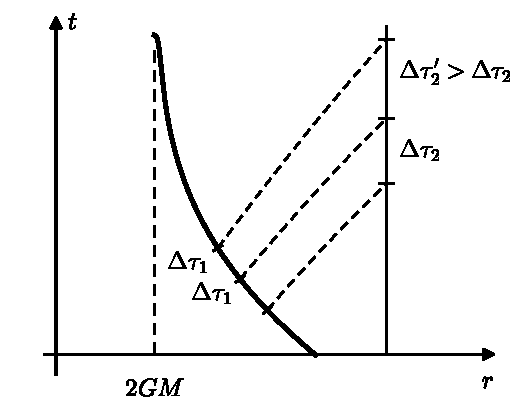
\includegraphics[width=0.72\textwidth]{fig_5.8.pdf}
\caption*{图 5.8\quad 自由落入黑洞的一个信标以恒定固有时间隔 $\Delta\tau_1$ 发出信号。固定 $r$ 处的观者收到信号的时间间隔 $\Delta\tau_2$ 依次变长。}
\end{figure}

% ---- 书页 220 / p235 ----
我们现有坐标的问题在于，沿接近 $r = 2GM$ 的径向类光测地线，$\mathrm{d}t/\mathrm{d}r \to \infty$；$r$ 方向上的推进相对于坐标时 $t$ 变得越来越慢。我们可以试着解决这个问题，办法是用一个沿类光测地线变化得更慢的坐标来取代 $t$。首先注意到，我们可以显式地解出刻画径向类光曲线的条件 (5.106)，得到
\begin{equation*}
t = \pm r^* + \text{constant},
\tag{5.107}
\end{equation*}
其中\textbf{乌龟坐标}（tortoise coordinate）$r^*$ 定义为
\begin{equation*}
r^* = r + 2GM\ln\left(\frac{r}{2GM} - 1\right).
\tag{5.108}
\end{equation*}
（乌龟坐标只有在 $r \geq 2GM$ 时才与 $r$ 有合理的关系，但反正在那个范围之外我们的坐标本来也不怎么好。）用乌龟坐标表示，Schwarzschild 度规变为
\begin{equation*}
\mathrm{d}s^2 = \left(1 - \frac{2GM}{r}\right)\left(-\mathrm{d}t^2 + \mathrm{d}r^{*2}\right) + r^2\,\mathrm{d}\Omega^2,
\tag{5.109}
\end{equation*}
其中 $r$ 被看作 $r^*$ 的函数。这代表了一些进展，因为如图 5.9 所示，光锥现在看起来不再闭合；此外，在 $r = 2GM$ 处没有任何度规系数变为无穷（尽管 $g_{tt}$ 和 $g_{r^* r^*}$ 都变为零）。然而我们付出的代价是，感兴趣的曲面 $r = 2GM$ 只是被推到了无限远。

我们的下一步行动，是定义自然地贴合类光测地线的坐标。若令
\begin{align*}
v &= t + r^*\\
u &= t - r^*,
\tag{5.110}
\end{align*}

\begin{figure}[H]
\centering
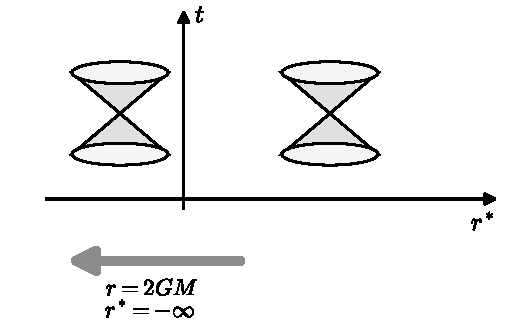
\includegraphics[width=0.72\textwidth]{fig_5.9.pdf}
\caption*{图 5.9\quad 乌龟坐标（式 (5.109)）下的 Schwarzschild 光锥。光锥保持非退化，但曲面 $r = 2GM$ 已被推到无限远。}
\end{figure}

% ---- 书页 221 / p236 ----
则落入的径向类光测地线由 $v =$ 常数刻画，而出射的径向类光测地线满足 $u =$ 常数。现在考虑回到原来的径向坐标 $r$，但用新坐标 $v$ 取代类时坐标 $t$。这组坐标就是所谓的\textbf{Eddington--Finkelstein 坐标}。用这组坐标表示，度规为
\begin{equation*}
\mathrm{d}s^2 = -\left(1 - \frac{2GM}{r}\right)\mathrm{d}v^2 + \left(\mathrm{d}v\,\mathrm{d}r + \mathrm{d}r\,\mathrm{d}v\right) + r^2\,\mathrm{d}\Omega^2.
\tag{5.111}
\end{equation*}
这里我们第一次看到了真正进展的迹象。尽管度规系数 $g_{vv}$ 在 $r = 2GM$ 处为零，但并不存在真正的退化；度规的行列式为
\begin{equation*}
g = -r^4\sin^2\theta,
\tag{5.112}
\end{equation*}
它在 $r = 2GM$ 处完全正则。因此度规是可逆的，而且我们一劳永逸地看到：在我们最初的 $(t, r, \theta, \phi)$ 坐标系中，$r = 2GM$ 只不过是一个坐标奇点。在 Eddington--Finkelstein 坐标中，径向类光曲线的条件解得
\begin{equation*}
\frac{\mathrm{d}v}{\mathrm{d}r} =
\begin{cases}
0, & \text{（落入）}\\[6pt]
2\left(1 - \dfrac{2GM}{r}\right)^{-1}. & \text{（出射）}
\end{cases}
\tag{5.113}
\end{equation*}
于是我们能够看清发生了什么：在这个坐标系中，光锥在 $r = 2GM$ 处依然表现良好，而且这个曲面位于有限的坐标值处。追踪类光或类时粒子穿过该曲面的路径没有任何问题。另一方面，确实有某种有趣的事情在发生。虽然光锥并不闭合，但它们确实倾倒了下来，使得当 $r < 2GM$ 时，所有指向未来的路径都指向 $r$ 减小的方向，如图 5.10 所示。

\begin{figure}[H]
\centering
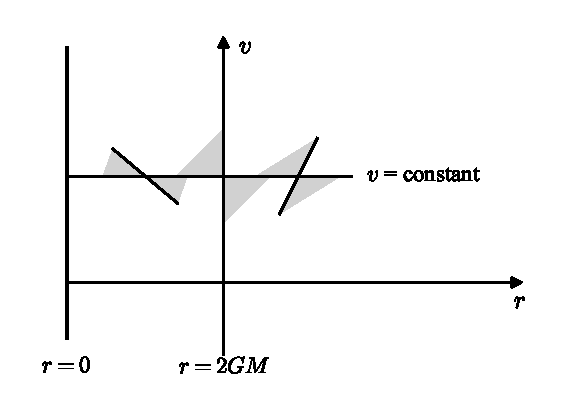
\includegraphics[width=0.72\textwidth]{fig_5.10.pdf}
\caption*{图 5.10\quad 式 (5.111) 的 $(v, r)$ 坐标下的 Schwarzschild 光锥。在这些坐标中，指向未来的类时路径可以越过 $r = 2GM$。}
\end{figure}

% ---- 书页 222 / p237 ----
曲面 $r = 2GM$ 虽然局部完全正则，但在整体上起着有去无回之点的作用——检验粒子一旦没入其内，就永远无法返回。我们把\textbf{事件视界}（event horizon）定义为粒子永远无法穿过它逃逸到无限远的曲面；在 Schwarzschild 时空中，事件视界位于 $r = 2GM$ 处。（这是一个粗略的定义；在下一章中我们会讲得稍微精确一些。）尽管位于固定的径向坐标处，事件视界却是一个类光曲面而非类时曲面，所以真正使得沿向外方向穿过视界成为不可能的，正是时空自身的因果结构。既然任何东西都无法逃出事件视界，我们也就不可能看到它的内部——这便是\textbf{黑洞}（black hole）这一名称的由来。黑洞不过是时空中的一个被事件视界与无限远分隔开的区域。事件视界的概念是一个整体性的概念；视界的位置是关于时空整体的陈述，不是仅知道该处的几何就能确定的。在更一般的时空中，这一点仍将成立。

我们应该提一下黑洞的几个在大众想象中常常被混淆的特点。首先，黑洞的外部几何与我们本会在恒星或行星之外得到的 Schwarzschild 解是同一个解。特别地，黑洞并不比太阳更会把周围的一切吸进去；在远离 $r = 2GM$ 之外的地方，无论引力源是不是黑洞，粒子的行为都完全一样。其次，关于黑洞存在一种误导性的 Newton 式类比。质量为 $M$ 的引力体外距离 $r$ 处的一个粒子，其 Newton 逃逸速度为
\begin{equation*}
v_{\mathrm{esc}} = \sqrt{\frac{2GM}{r}}.
\tag{5.114}
\end{equation*}
如果我们天真地问 Newton 逃逸速度在哪里等于光速，会发现恰好就是 $r = 2GM$。尽管光速在 Newton 理论中并不扮演任何基本角色，下面这件事看上去仍颇具挑衅意味：光——被当作以速度 $c$ 运动的惯性粒子——似乎无法从质量为 $M$、半径小于 $2GM$ 的天体逃出。但这种情况与我们在广义相对论中看到的存在深刻的差别。逃逸速度是粒子想要沿自由轨迹从引力源逃出时最初需要具有的速度；但没有什么能阻止我们考虑加速轨迹——比如，可以想象选取一个加速度，使得粒子以某个恒定的速度稳定地远离大质量天体。因此，假想的 Newton 黑洞将不会具有\emph{任何东西}都无法逃出这一关键性质；而在广义相对论中，任意的类时路径都必须待在各自的光锥之内，因而永远无法逃出事件视界。

\section{最大延拓的 Schwarzschild 解}

让我们回顾一下已经做了什么。出于对我们的坐标也许并不适用于整个流形的怀疑，我们已把原来的坐标 $t$ 换成了新坐标 $v$；后者的一个良好性质是，如果我们沿 $v =$ 常数的径向类光曲线减小 $r$，就会径直穿过事件视界而没有任何问题。

% ---- 书页 223 / p238 ----
的确，真正完成这趟旅行的局部观者未必知道事件视界是在何时被越过的——局部几何与其他任何地方并无不同。因此我们得出结论：我们的怀疑是对的，最初的坐标系未能很好地覆盖整个流形。区域 $r \leq 2GM$ 理所当然应当包含在我们的时空之中，因为物理粒子可以轻松到达并穿过那里。然而，这并不能保证我们已经大功告成；也许我们还能沿其他方向延拓流形。

实际上确实还有其他方向。在 $(v, r)$ 坐标系中，我们能够沿指向未来的路径穿过事件视界，却不能沿指向过去的路径。这显得不合情理，因为我们一开始面对的是一个不依赖时间的解。但我们本可以选择 $u$ 而不是 $v$，那样的话度规将是
\begin{equation*}
\mathrm{d}s^2 = -\left(1 - \frac{2GM}{r}\right)\mathrm{d}u^2 - \left(\mathrm{d}u\,\mathrm{d}r + \mathrm{d}r\,\mathrm{d}u\right) + r^2\,\mathrm{d}\Omega^2.
\tag{5.115}
\end{equation*}
现在我们又能穿过事件视界了，但这一次只能沿指向过去的曲线，如图 5.11 所示。

这也许令人惊讶：我们可以自洽地沿指向未来或指向过去的曲线穿过 $r = 2GM$，但会到达不同的地方。这其实本来就该预料到，因为从定义 (5.110) 看，如果保持 $v$ 不变而减小 $r$，必有 $t \to +\infty$；而如果保持 $u$ 不变而减小 $r$，则有 $t \to -\infty$。（当 $r \to 2GM$ 时，乌龟坐标 $r^* \to -\infty$。）于是我们沿两个不同的方向延拓了时空：一个朝向未来，一个朝向过去。

下一步本来可以沿着类空测地线走，看看是否还会发现更多的区域。答案是肯定的——我们会到达时空的另一块区域；不过让我们抄个近道，直接定义一组处处都好用的坐标。第一个猜测也许是同时使用 $u$ 和 $v$（来代替 $t$ 和 $r$），

\begin{figure}[H]
\centering
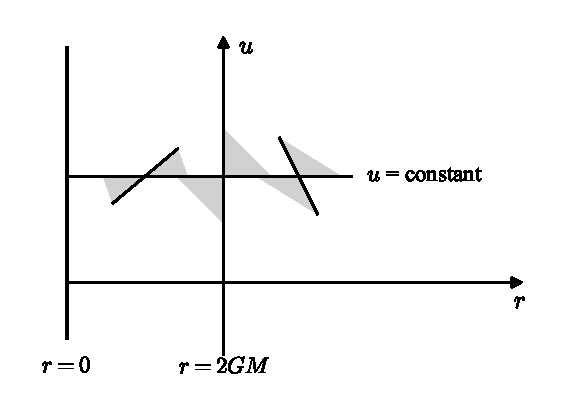
\includegraphics[width=0.72\textwidth]{fig_5.11.pdf}
\caption*{图 5.11\quad 式 (5.115) 的 $(u, r)$ 坐标下的 Schwarzschild 光锥。在这些坐标中，指向过去的类时路径可以越过 $r = 2GM$。}
\end{figure}

% ---- 书页 224 / p239 ----
这导致
\begin{equation*}
\mathrm{d}s^2 = -\frac{1}{2}\left(1 - \frac{2GM}{r}\right)\left(\mathrm{d}v\,\mathrm{d}u + \mathrm{d}u\,\mathrm{d}v\right) + r^2\,\mathrm{d}\Omega^2,
\tag{5.116}
\end{equation*}
其中 $r$ 通过下式由 $v$ 和 $u$ 隐式定义
\begin{equation*}
\frac{1}{2}(v - u) = r + 2GM\ln\left(\frac{r}{2GM} - 1\right).
\tag{5.117}
\end{equation*}
实际上，我们重新引入了一开始就带着的那种退化；在这些坐标中，$r = 2GM$ 又变得“无限遥远”（位于 $v = -\infty$ 或 $u = +\infty$ 处）。该做的事情是换用一组能把这些点拉回有限坐标值的坐标；一个很好的选择是
\begin{align*}
v' &= e^{v/4GM}\\
u' &= -e^{-u/4GM},
\tag{5.118}
\end{align*}
用我们原来的 $(t, r)$ 坐标系表示，即
\begin{align*}
v' &= \left(\frac{r}{2GM} - 1\right)^{1/2}e^{(r+t)/4GM}\\
u' &= -\left(\frac{r}{2GM} - 1\right)^{1/2}e^{(r-t)/4GM}.
\tag{5.119}
\end{align*}
在 $(v', u', \theta, \phi)$ 坐标系中，Schwarzschild 度规为
\begin{equation*}
\mathrm{d}s^2 = -\frac{16G^3M^3}{r}e^{-r/2GM}\left(\mathrm{d}v'\mathrm{d}u' + \mathrm{d}u'\mathrm{d}v'\right) + r^2\,\mathrm{d}\Omega^2.
\tag{5.120}
\end{equation*}
终于，$r = 2GM$ 的非奇异性变得完全显露出来；在这种形式下，在事件视界处没有任何度规系数表现出任何特殊的行为。

$v'$ 和 $u'$ 都是类光坐标，意思是它们的偏导数 $\partial/\partial v'$ 和 $\partial/\partial u'$ 是类光矢量。这本身并没有任何问题，因为这个坐标系中四个偏导数矢量（两个类光、两个类空）完全可以充当切空间的一组良好的基。尽管如此，在一个坐标类时、其余坐标类空的坐标系中工作还是要让人安心一些。于是我们定义
\begin{equation*}
T = \frac{1}{2}(v' + u') = \left(\frac{r}{2GM} - 1\right)^{1/2}e^{r/4GM}\sinh\left(\frac{t}{4GM}\right)
\tag{5.121}
\end{equation*}
以及
\begin{equation*}
R = \frac{1}{2}(v' - u') = \left(\frac{r}{2GM} - 1\right)^{1/2}e^{r/4GM}\cosh\left(\frac{t}{4GM}\right),
\tag{5.122}
\end{equation*}

% ---- 书页 225 / p240 ----
用它们表示，度规变为
\begin{equation*}
\boxed{\,\mathrm{d}s^2 = \frac{32G^3M^3}{r}e^{-r/2GM}\left(-\mathrm{d}T^2 + \mathrm{d}R^2\right) + r^2\,\mathrm{d}\Omega^2,\,}
\tag{5.123}
\end{equation*}
其中 $r$ 由下式隐式定义
\begin{equation*}
T^2 - R^2 = \left(1 - \frac{r}{2GM}\right)e^{r/2GM}.
\tag{5.124}
\end{equation*}
坐标 $(T, R, \theta, \phi)$ 被称为\textbf{Kruskal 坐标}（Kruskal coordinates），有时也称为 Kruskal--Szekeres 坐标。

Kruskal 坐标具有许多奇妙的性质。与 $(t, r^*)$ 坐标一样，径向类光曲线看起来与平直空间中相同：
\begin{equation*}
T = \pm R + \text{constant}.
\tag{5.125}
\end{equation*}
然而与 $(t, r^*)$ 坐标不同的是，事件视界 $r = 2GM$ 并不无限遥远；实际上它由下式定义
\begin{equation*}
T = \pm R,
\tag{5.126}
\end{equation*}
这与它是一个类光曲面相一致。更一般地，我们可以考虑 $r =$ 常数的曲面。由式 (5.124)，这些曲面满足
\begin{equation*}
T^2 - R^2 = \text{constant}.
\tag{5.127}
\end{equation*}
于是，它们在 $R$-$T$ 平面上呈现为一条条双曲线。此外，$t =$ 常数的曲面由下式给出
\begin{equation*}
\frac{T}{R} = \tanh\left(\frac{t}{4GM}\right),
\tag{5.128}
\end{equation*}
这定义了过原点、斜率为 $\tanh(t/4GM)$ 的直线。注意，当 $t \to \pm\infty$ 时，式 (5.128) 变得与式 (5.126) 相同；因此 $t = \pm\infty$ 与 $r = 2GM$ 代表同一个曲面。

我们的坐标 $(T, R)$ 应当被允许取遍它们在碰不到 $r = 0$ 处真实奇点的前提下所能取的一切值；因此允许的区域是
\begin{align*}
-\infty &\leq R \leq \infty\\
T^2 &< R^2 + 1.
\tag{5.129}
\end{align*}
由式 (5.121) 和 (5.122)，当 $r < 2GM$ 时 $T$ 和 $R$ 似乎会成为虚数，但这是一种错觉；在那个区域里 $(r, t)$ 坐标本来就不好用（具体地说，$|t| > \infty$）。现在我们可以在 $T$-$R$ 平面上（隐去 $\theta$ 和 $\phi$）画出一幅时空图，即所谓的\textbf{Kruskal 图}（Kruskal diagram），如图 5.12 所示。图上的每个点都是一个二维球面。这幅图表示的就是 Schwarzschild 几何的最大延拓，

% ---- 书页 226 / p241 ----
\begin{figure}[H]
\centering
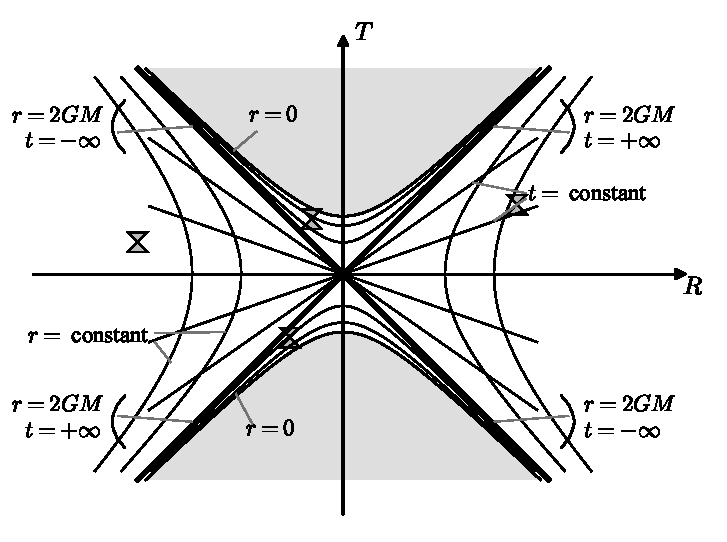
\includegraphics[width=0.72\textwidth]{fig_5.12.pdf}
\caption*{图 5.12\quad Kruskal 图——Kruskal 坐标下的 Schwarzschild 解，其中所有光锥都张开 $\pm 45^{\circ}$。}
\end{figure}

这些坐标所覆盖的，正是我们应当看作由这个解所描述的整个流形。

原来的 Schwarzschild 坐标 $(t, r)$ 只在 $r > 2GM$ 时好用，而这只是 Kruskal 图上所描绘的流形的一部分。把图分成四个区域会带来方便，如图 5.13 所示。区域 I 对应于 $r > 2GM$，即我们原来的坐标在其中具有良好定义的那一片。沿着指向未来的类光射线，我们到达区域 II；沿着指向过去的类光射线，则到达区域 III。如果当初探索的是类空测地线，就会被引到区域 IV。把 $(T, R)$ 与 $(t, r)$ 联系起来的定义 (5.121) 和 (5.122) 实际上只在区域 I 中好用；在其他区域中，必须引入适当的负号，以防止坐标变成虚数。

\begin{figure}[H]
\centering
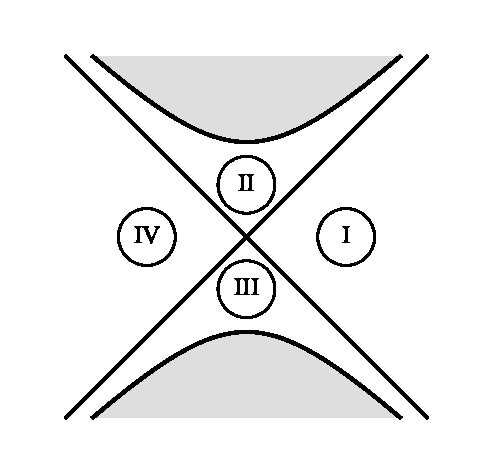
\includegraphics[width=0.72\textwidth]{fig_5.13.pdf}
\caption*{图 5.13\quad Kruskal 图的各个区域。}
\end{figure}

% ---- 书页 227 / p242 ----
把 Schwarzschild 几何延拓到所能延拓的极致之后，我们描述了一个不同凡响的时空。当然，区域 II 就是我们所说的黑洞。任何东西一旦从区域 I 进入区域 II，就再也回不来了。实际上，区域 II 中每一条指向未来的路径最终都会撞上 $r = 0$ 处的奇点；一旦进入事件视界，你就在劫难逃。这一点值得强调：你不仅无法逃回区域 I，甚至无法让自己停止沿 $r$ 减小的方向运动，因为这恰恰是类时方向。这一点本来也可以在原来的坐标系中看出来：当 $r < 2GM$ 时，$t$ 变成类空的，而 $r$ 变成类时的。因此，你无法停止向奇点运动，就像你无法停止变老一样。由于固有时沿测地线取极大值，如果你不作挣扎，而是放松身体接近奇点，你就能活得最久。倒不是说你还有多久可以放松，这趟旅程也谈不上令人松弛：当你接近奇点时，潮汐力会变得无穷大。当你落向奇点时，你的脚和头会被彼此拉开，而你的躯干则被挤压到无穷薄。一位天体物理学家落入黑洞后的凄惨下场，在 Misner、Thorne 与 Wheeler (1973) 的第 32.6 节中有细致的描述。注意他们使用了正交归一标架，正如我们在附录 J 中讨论的那样（不过这可不会让这趟旅行变得更愉快）。

区域 III 和区域 IV 可能有些出乎意料。区域 III 不过是区域 II 的时间反演，是时空中这样一个部分：其中的东西可以逃到我们这里，而我们却永远到不了那里。它可以被看作一个\textbf{白洞}（white hole）。在过去存在一个奇点，宇宙看起来正是从那里迸发而出的。区域 III 的边界是过去事件视界，而区域 II 的边界是未来事件视界。至于区域 IV，无论沿时间向前还是向后，都无法从我们的区域 I 到达那里，那边的人也同样无法到我们这里来。它是时空的另一个渐近平直区域，是我们这个区域的镜像。可以认为它通过一个虫洞（wormhole，或称 Einstein--Rosen 桥）与区域 I 相连——这是一种连接两个不同区域的瓶颈状结构。考虑把 Kruskal 图按 $T =$ 常数的类空曲面切片，如图 5.14 所示。现在我们可以把每个切片的图像画出来，为清晰起见把一个角坐标也画上，如图 5.15 那样。按这种切片方式，Schwarzschild 几何描述的是两个渐近平直的区域：它们相互伸向对方，经由虫洞连接一段时间，然后再断开。但虫洞闭合得太快，任何类时观者都来不及从一个区域穿过它进入另一个区域。

尽管 Kruskal 图已经令人赏心悦目，通过构造共形图把 Schwarzschild 解压缩到有限区域之内，往往还要更有用。共形图的思想在附录 H 中讨论；它是分析广义相对论中时空的关键工具，建议你现在就把那里的讨论复习一遍。我们不会完整详尽地给出构造 Schwarzschild 共形图所必需的那些操作，因为它们与 Minkowski 情形如出一辙，只是代数上额外复杂了不少。我们会从类光版本的 Kruskal 坐标出发，在其中度规

% ---- 书页 228 / p243 ----
\begin{figure}[H]
\centering
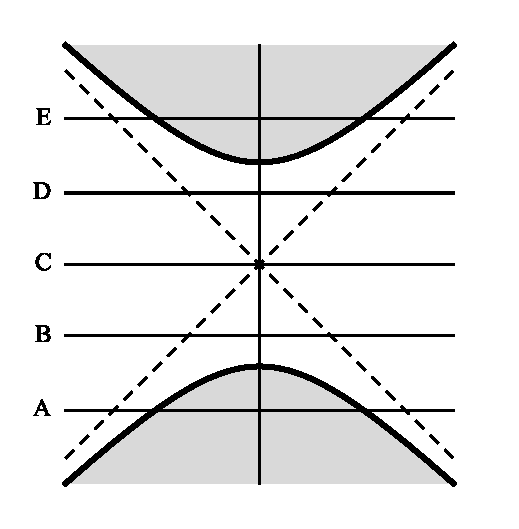
\includegraphics[width=0.72\textwidth]{fig_5.14.pdf}
\caption*{图 5.14\quad Kruskal 坐标中的类空切片。}
\end{figure}

取如下形式
\begin{equation*}
\mathrm{d}s^2 = -\frac{16G^3M^3}{r}e^{-r/2GM}\left(\mathrm{d}v'\mathrm{d}u' + \mathrm{d}u'\mathrm{d}v'\right) + r^2\,\mathrm{d}\Omega^2,
\tag{5.130}
\end{equation*}
其中 $r$ 通过下式隐式定义
\begin{equation*}
v'u' = -\left(\frac{r}{2GM} - 1\right)e^{r/2GM}.
\tag{5.131}
\end{equation*}
然后，基本上照搬平直时空情形中用过的同一个变换，就足以把无限远收进有限的坐标值：
\begin{align*}
v'' &= \arctan\left(\frac{v'}{\sqrt{2GM}}\right)\\
u'' &= \arctan\left(\frac{u'}{\sqrt{2GM}}\right),
\tag{5.132}
\end{align*}

\begin{figure}[H]
\centering
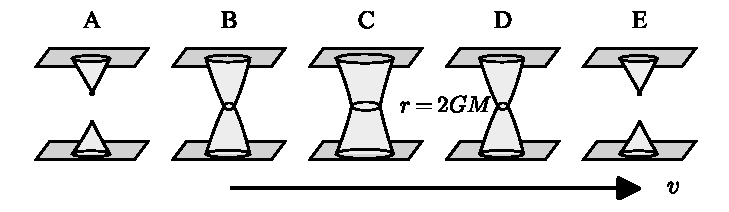
\includegraphics[width=0.72\textwidth]{fig_5.15.pdf}
\caption*{图 5.15\quad 图 5.14 中诸类空切片的几何。}
\end{figure}
范围为
% ---- 书页 229 / p244 ----
\begin{gather*}
-\frac{\pi}{2} < v'' < +\frac{\pi}{2}\\
-\frac{\pi}{2} < u'' < +\frac{\pi}{2}\\
-\frac{\pi}{2} < v'' + u'' < \frac{\pi}{2}.
\end{gather*}

\begin{figure}[H]
\centering
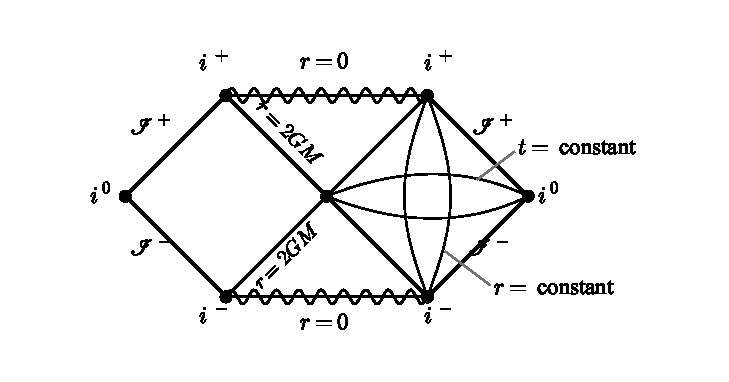
\includegraphics[width=0.72\textwidth]{fig_5.16.pdf}
\caption*{图 5.16\quad Schwarzschild 时空的共形图。}
\end{figure}

度规的 $(v'', u'')$ 部分（也就是说，在角坐标为常数的情形下）现在与 Minkowski 空间共形相关。在新坐标中，$r=0$ 处的奇点是一些直线，它们从一个渐近区域的类时无限远一直延伸到另一个渐近区域的类时无限远。

于是，极大延拓的 Schwarzschild 解的共形图看上去就像图 5.16 那样。这幅图唯一真正微妙的地方，在于必须理解 $i^+$ 和 $i^-$（未来和过去无限远）与 $r=0$ 是彼此不同的——存在大量不会撞上奇点的类时路径。正如 Kruskal 图中那样，共形图中的光锥也张开 $45^{\circ}$；主要的不同在于，整个时空被表示在一个有限的区域之内。还要注意，共形无限远的结构与 Minkowski 空间的结构一模一样，这与 Schwarzschild 时空渐近平直的论断相一致。

\section{恒星与黑洞}

我们刚刚构造的极大延拓 Schwarzschild 解讲述了一个不同凡响的故事：其中不仅有我们苦苦寻找的黑洞，还有白洞，以及另一个通过虫洞与我们宇宙相连的渐近平直区域。然而，设想这些特征在真实世界中十分常见，还为时过早。Schwarzschild 解代表的是一种高度理想化的情形：它不仅球对称，而且在整个时空中完全不含能量-动量。Birkhoff 定理意味着，球对称时空的任何真空\emph{区域}都将由 Schwarzschild 度规的\emph{一部分}来描述，但宇宙中某处物质的存在可能会戏剧性地改变整体的图像。

% ---- 书页 230 / p245 ----
一个静态的球状物体——为明确起见，就把它叫作恒星——如果半径大于 $2GM$，其外部将是 Schwarzschild 的，但不会有任何奇点或视界，而且整体结构实际上与 Minkowski 时空非常相似。当然，真实的恒星会演化，恒星有可能最终在自身引力的拉拽下坍缩，收缩到 $r=2GM$ 以下，进而落入奇点，形成黑洞。然而，这并不需要白洞，因为这样一个时空的过去与完整 Schwarzschild 解的过去毫无相似之处。描绘恒星坍缩的共形图看上去会像图 5.17 那样。内部的阴影区域不是真空，因此不由 Schwarzschild 度规描述；特别地，不存在连接到另一个宇宙的虫洞。这个时空是渐近 Minkowski 型的，只是未来的一个区域会生成事件视界。我们看到，真实的黑洞可以与极大延拓的 Schwarzschild 解共有奇点和未来视界，而不带任何白洞、过去视界或另外的渐近区域。

我们相信，这类引力坍缩绝不是恒星演化的必然终点，但在一定条件下将会发生。广义相对论对能够抵抗引力坍缩的恒星种类给出了严格的限制；对任何给定种类的物质，足够大的质量总会导致坍缩为黑洞。此外，从天体物理观测中我们已有了极好的证据，表明黑洞存在于我们的宇宙之中。

为了理解向黑洞的引力坍缩，我们应当首先理解描述球对称恒星内部的静态位形。我们不打算深入钻研这个专题，只需对内解的基本特征获得一点感觉就够了。考虑取自式 (5.11) 的一般静态、球对称度规：

\begin{figure}[H]
\centering
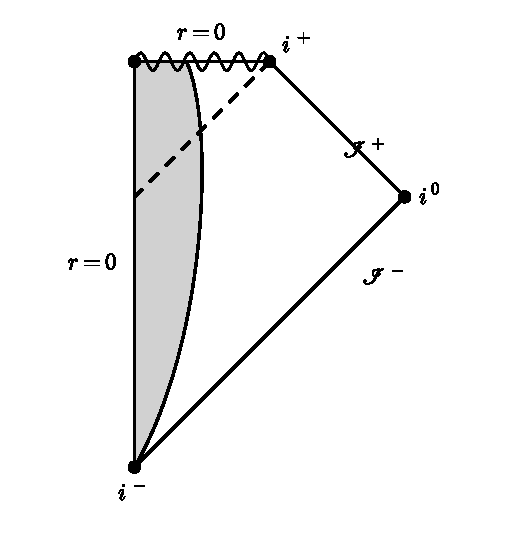
\includegraphics[width=0.72\textwidth]{fig_5.17.pdf}
\caption*{图 5.17\quad 由坍缩恒星形成的黑洞的共形图。阴影区域包含物质，将由某个适当的动力学内解来描述；外部区域则是 Schwarzschild 的。}
\end{figure}

% ---- 书页 231 / p246 ----
\begin{equation*}
\mathrm{d}s^2 = -e^{2\alpha(r)}\,\mathrm{d}t^2 + e^{2\beta(r)}\,\mathrm{d}r^2 + r^2\,\mathrm{d}\Omega^2.
\tag{5.133}
\end{equation*}
我们现在寻找的是非真空解，因此转向完整的 Einstein 方程，
\begin{equation*}
G_{\mu\nu} = R_{\mu\nu} - \frac{1}{2}R g_{\mu\nu} = 8\pi G\,T_{\mu\nu}.
\tag{5.134}
\end{equation*}
Einstein 张量可由 Ricci 张量 (5.14) 与标量曲率 (5.15) 得到，
\begin{align*}
G_{tt} &= \frac{1}{r^2}e^{2(\alpha-\beta)}\left(2r\,\partial_r\beta - 1 + e^{2\beta}\right)\\
G_{rr} &= \frac{1}{r^2}\left(2r\,\partial_r\alpha + 1 - e^{2\beta}\right)\\
G_{\theta\theta} &= r^2 e^{-2\beta}\left[\partial_r^2\alpha + (\partial_r\alpha)^2 - \partial_r\alpha\,\partial_r\beta + \frac{1}{r}(\partial_r\alpha - \partial_r\beta)\right]\\
G_{\phi\phi} &= \sin^2\theta\, G_{\theta\theta}.
\tag{5.135}
\end{align*}
我们把恒星本身建模为理想流体，其能动张量为
\begin{equation*}
T_{\mu\nu} = (\rho + p)U_\mu U_\nu + p\,g_{\mu\nu}.
\tag{5.136}
\end{equation*}
能量密度 $\rho$ 与压强 $p$ 将只是 $r$ 的函数。既然我们寻求的是静态解，就可以取四速度指向类时方向。归一化到 $U^\mu U_\mu = -1$，它便成为
\begin{equation*}
U_\mu = (e^{\alpha},\, 0,\, 0,\, 0),
\tag{5.137}
\end{equation*}
于是能动张量的分量为
\begin{equation*}
T_{\mu\nu} =
\begin{pmatrix}
e^{2\alpha}\rho & & & \\
& e^{2\beta}p & & \\
& & r^2 p & \\
& & & r^2(\sin^2\theta)p
\end{pmatrix}.
\tag{5.138}
\end{equation*}
这样我们便得到 Einstein 方程的三个独立分量：$tt$ 分量，
\begin{equation*}
\frac{1}{r^2}e^{-2\beta}\left(2r\,\partial_r\beta - 1 + e^{2\beta}\right) = 8\pi G\rho,
\tag{5.139}
\end{equation*}
$rr$ 分量，
\begin{equation*}
\frac{1}{r^2}e^{-2\beta}\left(2r\,\partial_r\alpha + 1 - e^{2\beta}\right) = 8\pi Gp,
\tag{5.140}
\end{equation*}

% ---- 书页 232 / p247 ----
以及 $\theta\theta$ 分量，
\begin{equation*}
e^{-2\beta}\left[\partial_r^2\alpha + (\partial_r\alpha)^2 - \partial_r\alpha\,\partial_r\beta + \frac{1}{r}(\partial_r\alpha - \partial_r\beta)\right] = 8\pi Gp.
\tag{5.141}
\end{equation*}
$\phi\phi$ 方程与 $\theta\theta$ 方程成比例，因此不必单独考虑。

我们注意到，$tt$ 方程 (5.139) 只涉及 $\beta$ 和 $\rho$。用一个新的函数 $m(r)$ 来取代 $\beta(r)$ 会带来方便，$m(r)$ 定义为
\begin{equation*}
m(r) = \frac{1}{2G}\left(r - re^{-2\beta}\right),
\tag{5.142}
\end{equation*}
或者等价地
\begin{equation*}
e^{2\beta} = \left[1 - \frac{2Gm(r)}{r}\right]^{-1},
\tag{5.143}
\end{equation*}
于是
\begin{equation*}
\mathrm{d}s^2 = -e^{2\alpha(r)}\,\mathrm{d}t^2 + \left[1 - \frac{2Gm(r)}{r}\right]^{-1}\mathrm{d}r^2 + r^2\,\mathrm{d}\Omega^2.
\tag{5.144}
\end{equation*}
度规分量 $g_{rr}$ 显然是 Schwarzschild 情形的直接推广，但 $g_{tt}$ 却不是这样。$tt$ 方程 (5.139) 变为
\begin{equation*}
\frac{dm}{dr} = 4\pi r^2\rho,
\tag{5.145}
\end{equation*}
积分可得
\begin{equation*}
m(r) = 4\pi\int_0^r \rho(r')r'^2\,\mathrm{d}r'.
\tag{5.146}
\end{equation*}
设想我们的恒星延伸到半径 $R$ 处，在此之外是真空，由 Schwarzschild 度规描述。为了使度规在这个半径处匹配，Schwarzschild 质量 $M$ 必须为
\begin{equation*}
M = m(R) = 4\pi\int_0^R \rho(r)r^2\,\mathrm{d}r.
\tag{5.147}
\end{equation*}
看起来，$m(r)$ 不过是能量密度在恒星内部的一个积分，可以解释为半径 $r$ 以内的质量。

把 $m(r)$ 解释为积分能量密度时有一个微妙之处；在一个适当的空间积分中，体积元应当是
\begin{equation*}
\sqrt{\gamma}\,\mathrm{d}^3x = e^{\beta}r^2\sin\theta\,\mathrm{d}r\,\mathrm{d}\theta\,\mathrm{d}\phi,
\tag{5.148}
\end{equation*}
其中
\begin{equation*}
\gamma_{ij}\,\mathrm{d}x^i\mathrm{d}x^j = e^{2\beta}\,\mathrm{d}r^2 + r^2\,\mathrm{d}\theta^2 + r^2\sin^2\theta\,\mathrm{d}\phi^2
\tag{5.149}
\end{equation*}

% ---- 书页 233 / p248 ----
便是空间度规。因此，真正的积分能量密度是
\begin{align*}
\bar{M} &= 4\pi\int_0^R \rho(r)r^2 e^{\beta(r)}\,\mathrm{d}r\\
&= 4\pi\int_0^R \frac{\rho(r)r^2}{\left[1 - \dfrac{2Gm(r)}{r}\right]^{1/2}}\,\mathrm{d}r.
\tag{5.150}
\end{align*}
当然，这个差别来自结合能：恒星内流体元之间的相互引力吸引产生了一种结合能，它由下式给出
\begin{equation*}
E_{\mathrm{B}} = \bar{M} - M > 0.
\tag{5.151}
\end{equation*}
结合能是把恒星中的物质驱散到无限远所需要的能量。在广义相对论中它并不总是一个有良定义的概念，但对球状恒星来说是有意义的。

用 $m(r)$ 来表示，$rr$ 方程 (5.140) 可以写成
\begin{equation*}
\frac{d\alpha}{dr} = \frac{Gm(r) + 4\pi G r^3 p}{r\left[r - 2Gm(r)\right]}.
\tag{5.152}
\end{equation*}
不直接使用 $\theta\theta$ 方程，而是转而借助能量-动量守恒 $\nabla_\mu T^{\mu\nu} = 0$，会更加方便。对我们的度规 (5.144)，容易推出 $\nu = r$ 是唯一非平庸的分量，它给出
\begin{equation*}
(\rho + p)\frac{d\alpha}{dr} = -\frac{dp}{dr}.
\tag{5.153}
\end{equation*}
把它与 (5.152) 联立，就可以消去 $\alpha(r)$，得到
\begin{equation*}
\frac{dp}{dr} = -\frac{(\rho + p)\left[Gm(r) + 4\pi G r^3 p\right]}{r\left[r - 2Gm(r)\right]}.
\tag{5.154}
\end{equation*}
这就是\textbf{Tolman--Oppenheimer--Volkoff 方程}，或简称流体静力学平衡方程。由于 $m(r)$ 通过 (5.146) 与 $\rho(r)$ 相联系，这个方程便把 $p(r)$ 与 $\rho(r)$ 联系了起来。为了得到一个封闭的方程组，我们还需要一个关系：物态方程。一般而言，它以能量密度和比熵给出压强，$p = p(\rho, S)$。我们关心的常常是熵非常小、从而可以忽略的情形；此时物态方程便取如下形式
\begin{equation*}
p = p(\rho).
\tag{5.155}
\end{equation*}
天体物理系统常常服从多方物态方程（polytropic equation of state）$p = K\rho^{\gamma}$，其中 $K$ 和 $\gamma$ 是常数。

一个简单而半现实的恒星模型来自如下假设：流体是不可压缩的——密度为常数 $\rho_*$，一直保持到恒星表面，过了表面它便为零，

% ---- 书页 234 / p249 ----
即
\begin{equation*}
\rho(r) =
\begin{cases}
\rho_*, & r < R\\
0, & r > R.
\end{cases}
\tag{5.156}
\end{equation*}
显式地给定 $\rho(r)$ 便顶替了物态方程，因为 $p(r)$ 可以由流体静力学平衡确定。接下来直接积分 (5.146) 就得到
\begin{equation*}
m(r) =
\begin{cases}
\dfrac{4}{3}\pi r^3\rho_*, & r < R\\[8pt]
\dfrac{4}{3}\pi R^3\rho_* = M, & r > R.
\end{cases}
\tag{5.157}
\end{equation*}
对流体静力学平衡方程积分，给出
\begin{equation*}
p(r) = \rho_*\left[\frac{R\sqrt{R-2GM} - \sqrt{R^3-2GMr^2}}{\sqrt{R^3-2GMr^2} - 3R\sqrt{R-2GM}}\right].
\tag{5.158}
\end{equation*}
最后我们可以由 (5.152) 得到度规分量 $g_{tt} = -e^{2\alpha(r)}$；我们发现
\begin{equation*}
e^{\alpha(r)} = \frac{3}{2}\left(1 - \frac{2GM}{R}\right)^{1/2} - \frac{1}{2}\left(1 - \frac{2GMr^2}{R^3}\right)^{1/2}, \quad r < R.
\tag{5.159}
\end{equation*}
正如所期待的那样，压强在恒星核心附近增大。实际上，对固定半径 $R$ 的恒星，如果质量超过
\begin{equation*}
M_{\mathrm{max}} = \frac{4}{9G}R.
\tag{5.160}
\end{equation*}
中心压强 $p(0)$ 就必须大于无穷大。

因此，如果我们试图把比这更大的质量挤进半径 $R$ 之内，广义相对论便不允许任何静态解；收缩到这种尺寸的恒星必然要继续收缩，最终形成一个黑洞。我们是在密度为常数这个相当强的假设下导出这一结果的，但当这一假设被大大放宽后它依然成立；\textbf{Buchdahl 定理}断言，任何合理的静态球对称内解都满足 $M < 4R/9G$。虽然严格的证明需要更多的工作，这个结果是说得通的；设想自然界存在某个最大可维持的密度，那么原则上我们所能造出的质量最大的物体将处处具有这一密度，而这正是我们考虑过的那个具体情形。

当然，这仍然不意味着现实的天体物理客体最终总会坍缩为黑洞。一颗依靠物质压强支撑的普通行星，基本上会永远存续下去（除非出现某些概率低得离谱的量子隧穿——一颗行星隧穿成某种截然不同的东西——或者最终发生质子衰变的可能性）。但大质量恒星就是另一回事了。支撑恒星的压强来自轻核聚合成较重核所产生的热量。当核燃料耗尽时，温度下降，恒星便开始在引力的作用下收缩。

% ---- 书页 235 / p250 ----
坍缩最终可能被 Fermi 简并压强止住：电子被挤得如此靠近，以至于单凭 Pauli 不相容原理（不能有两个费米子处于同一个态），它们便能抵抗进一步的压缩。靠电子简并压强支撑的恒星遗骸称为\textbf{白矮星}（white dwarf）；典型的白矮星在大小上与地球相当。质量较小的粒子在比高质量粒子更低的数密度下就会变得简并，因此核子对白矮星中的压强没有可观的贡献。白矮星是大多数恒星的最终状态，在整个宇宙中极为常见。

然而，如果总质量足够高，恒星将达到\textbf{Chandrasekhar 极限}，在那里连电子简并压强也不足以抵抗引力的拉拽。计算给出的 Chandrasekhar 极限约为 $1.4\,M_{\odot}$，其中 $M_{\odot} = 2\times 10^{33}$ g 是太阳的质量。一旦达到这一极限，恒星就被迫坍缩到更小的半径。在这一点上，电子与质子结合生成中子和中微子（逆 $\beta$ 衰变），而中微子则径直飞走。其结果是一颗\textbf{中子星}（neutron star），典型半径约为 10 km。中子星的总光度很低，但往往快速自转并具有强磁场。这种组合催生了\textbf{脉冲星}（pulsar）：它们沿着从磁极发出的喷流加速粒子，随着中子星的自转，看起来在迅速地闪烁。脉冲星由 Bell 于 1967 年发现；在短暂地猜测它们或许代表来自某个地外文明的信号之后，人们最终接受了这个更为平淡的天体物理解释。

由于中子星中心处的条件与地球上的条件非常不同，我们对物态方程的理解并不完美。尽管如此，我们相信质量足够大的中子星自身将无法抵抗引力的拉拽，并将继续坍缩；目前对中子星最大可能质量的估计在 $3$--$4\,M_{\odot}$ 左右，即\textbf{Oppenheimer--Volkoff 极限}。由于中子流体是我们所知最致密的物质（除了某些非常思辨性的设想），人们相信这种坍缩的结局是一个黑洞。

如果真有黑洞，我们会怎样知道它的存在？直接探测的根本障碍当然在于黑暗：黑洞本身不会发出任何辐射（忽略霍金辐射——那是一个非常小的效应，我们将在第 9 章讨论）。但黑洞带有极强的引力场，所以我们有望通过观测受这些场影响的物质来间接探测它们。物质落入黑洞时会升温并发出 X 射线，我们可以用卫星天文台探测到这些射线。用这种方法已经探测到大量黑洞候选体，我们宇宙中存在真实黑洞的证据是极其有力的。\footnote{关于黑洞的天体物理证据的综述，见 A.~Celotti、J.C.~Miller 与 D.W.~Sciama (1999)，\emph{Class.~Quant.~Grav.}~\textbf{16}, A3；\texttt{http://arxiv.org/abs/astro-ph/9912186}。}绝大多数候选体属于以下两类之一。一类是质量为太阳质量量级或略高一些的黑洞；它们被认为是质量非常大的恒星演化的终点。另一类描述超大质量黑洞（supermassive black holes），
% ---- 书页 236 / p251 ----
质量介于 $10^6$ 到 $10^9$ 个太阳质量之间。它们位于星系的中心，被认为是星系形成早期驱动类星体的引擎。我们自己的银河系就包含一个天体（Sgr A$^*$），据信它是一个质量至少为 $2\times 10^6\,M_{\odot}$ 的黑洞。这些超大质量黑洞形成的确切历史还不甚清楚。其他可能性还包括产生于极早期宇宙的非常小的原初黑洞（primordial black holes），以及所谓的“中量级”黑洞——质量在约一千个太阳质量量级。

物质落入黑洞时，往往会安定下来形成一个旋转的吸积盘（accretion disk），能量和角动量都随之逐渐注入洞中。因此，我们预期在天体物理情形中看到的黑洞应当是旋转的，而且观测确实与已观测到的黑洞具有非常高的自转速率相一致。在本章中，我们通过聚焦于球对称的 Schwarzschild 解排除了黑洞自转的可能性；下一章我们将转向更一般类型的黑洞。

\section{习题}

% 习题编号照原书
\textbf{1.}\quad 一只太空猴子正快乐地沿一条圆形测地线轨道绕着一个 Schwarzschild 黑洞运转。一只邪恶的狒狒在远离黑洞的地方，企图把一颗时机经过精心计算的椰子沿径向投向黑洞，好把猴子送进黑洞内部置于死地——它知道猴子无法抗拒要接住那颗下落椰子的冲动。给定猴子的质量与初始轨道半径以及椰子的质量，请说明你打算如何着手求解这个问题（但不必真的把计算做出来）。我们这位无畏的太空猴子可能落得怎样的命运？

\textbf{2.}\quad 考虑静态、圆对称的 $(2+1)$ 维时空中的一个理想流体；等价地说，即 $(3+1)$ 维中具有完全转动对称性的一个柱状位形。

\textbf{(a)}\quad 推导 $(2+1)$ 维情形下 Tolman--Oppenheimer--Volkoff（TOV）方程的类似物。

\textbf{(b)}\quad 证明真空解可以写成
\begin{equation*}
\mathrm{d}s^2 = -\mathrm{d}t^2 + \frac{1}{1-8GM}\,\mathrm{d}r^2 + r^2\,\mathrm{d}\theta^2
\end{equation*}
这里 $M$ 是常数。

\textbf{(c)}\quad 证明同一个解还有另一种写法
\begin{equation*}
\mathrm{d}s^2 = -\mathrm{d}\tau^2 + \mathrm{d}\xi^2 + \xi^2\,\mathrm{d}\phi^2
\end{equation*}
其中 $\phi\in\left[0,\,2\pi(1-8GM)^{1/2}\right]$。

\textbf{(d)}\quad 对一颗常密度恒星求解 $(2+1)$ 维 TOV 方程。求出 $p(r)$ 并解出度规。

\textbf{(e)}\quad 对具有物态方程 $p = \kappa\rho^{3/2}$ 的恒星求解 $(2+1)$ 维 TOV 方程。求出 $p(r)$ 并解出度规。

\textbf{(f)}\quad 对 (d)、(e) 两个小题中的解，求质量 $M(R) = \int_0^{2\pi}\int_0^R \rho\,\mathrm{d}r\,\mathrm{d}\theta$ 以及固有质量 $\bar{M}(R) = \int_0^{2\pi}\int_0^R \rho\sqrt{-g}\,\mathrm{d}r\,\mathrm{d}\theta$。

% ---- 书页 237 / p252 ----
\textbf{3.}\quad 考虑一个已经落入事件视界之内（$r < 2GM$）的粒子（不一定沿测地线运动）。使用通常的 Schwarzschild 坐标 $(t, r, \theta, \phi)$。试证明径向坐标必须以下式给出的最小速率减小：
\begin{equation*}
\left|\frac{\mathrm{d}r}{\mathrm{d}\tau}\right| \geq \sqrt{\frac{2GM}{r} - 1}.
\end{equation*}
计算一个粒子沿从 $r = 2GM$ 到 $r = 0$ 的轨迹所能具有的最大寿命。对质量以太阳质量计的黑洞，把这个结果用秒表示出来。试证明这一最大固有时是通过 $E \to 0$ 的自由下落实现的。

\textbf{4.}\quad 考虑真空中的 Einstein 方程，但带有一个宇宙学常数：$G_{\mu\nu} + \Lambda g_{\mu\nu} = 0$。

\textbf{(a)}\quad 求出最一般的球对称度规，所用的 $(t, r)$ 坐标在 $\Lambda = 0$ 时退化为通常的 Schwarzschild 坐标。

\textbf{(b)}\quad 像式 (5.66) 那样，用有效势写出径向测地线的运动方程。概略画出有质量粒子的有效势。

\textbf{5.}\quad 考虑一个共动观者，静止在质量为 $M$ 的 Schwarzschild 黑洞周围恒定的空间坐标 $(r_*, \theta_*, \phi_*)$ 处。该观者把一个信标投入黑洞（径直向下，沿径向轨迹）。信标以恒定波长 $\lambda_{\mathrm{em}}$（在信标静止系中）发出辐射。

\textbf{(a)}\quad 计算信标的坐标速度 $\mathrm{d}r/\mathrm{d}t$，表示为 $r$ 的函数。

\textbf{(b)}\quad 计算信标的固有速度。也就是说，设想在固定的 $r$ 处有一个共动观者，在信标经过时建立起一个局部惯性坐标系，试计算这个共动观者所测得的速度。它在 $r = 2GM$ 处是多少？

\textbf{(c)}\quad 计算由 $r_*$ 处的观者测得的波长 $\lambda_{\mathrm{obs}}$，表示为辐射被发射处半径 $r_{\mathrm{em}}$ 的函数。

\textbf{(d)}\quad 计算信标在半径 $r_{\mathrm{em}}$ 处发出的一束辐射将于 $r_*$ 处被观测到的时刻 $t_{\mathrm{obs}}$。

\textbf{(e)}\quad 试证明在很晚的时刻，红移按指数增长：$\lambda_{\mathrm{obs}}/\lambda_{\mathrm{em}} \propto e^{t_{\mathrm{obs}}/T}$。给出时间常数 $T$ 用黑洞质量 $M$ 表示的表达式。

% 第5章正文至此结束（原书书页 237 末；书页 238 起为第 6 章）。

 % 本文件由 scripts/assemble.py 自动装配，勿手改（改 parts/ 后重跑）
% 第6章 更一般的黑洞

% 第6章 More General Black Holes
\chapter{更一般的黑洞}

\section{黑洞动物园}

% ---- 书页 238 / p253 ----
Birkhoff 定理保证了 Schwarzschild 度规是广义相对论中唯一的球对称真空解。这并不太令人惊讶，因为它让我们想起电磁学中的情形：在无电荷的区域里，唯一的球对称场位形就是 Coulomb 场。走出球对称性之后，可能的引力场就五花八门、不胜枚举。比如对一颗像地球这样的行星，其外部场将依赖于表面上所有各种山脉与山谷的密度和轮廓。我们可以设想把度规按多极矩（multipole moments）展开；要精确描述这个场，就得给定无穷多个系数。

因此，黑洞并不具备这种性质，这一点或许反倒会让人感到几分意外。稳态黑洞解只有寥寥几个，每个解由少数几个参量描述。参量的具体集合取决于我们的理论中包含哪些物质场；如果电磁学是唯一的长程非引力场，我们就有一条\textbf{无毛定理}（no-hair theorem）：

与电磁学相耦合的广义相对论的稳态、渐近平直黑洞解，只要在事件视界之外无奇点，就完全由质量、电荷与磁荷以及角动量这几个参量刻画。

稳态解之所以特别令人感兴趣，是因为我们预期它们是引力坍缩的终态。另一种可能是某种振荡的位形，但随着能量通过引力辐射的发射而损耗，振荡终将被阻尼；实际上，典型的演化会相当迅速地趋于稳态位形。

我们说的是“一条”无毛定理，而不是“那条”无毛定理，因为这一结果不仅依赖于广义相对论，还依赖于我们理论中的物质内容。在粒子物理的标准模型中，电磁学是唯一的长程场，上面的定理适用；但对别的种类的场来说，可能存在其他种类的毛发。\footnote{相关讨论见 M. Heusler, “Stationary Black Holes: Uniqueness and Beyond,” \emph{Living Rev.\ Relativity} \textbf{1} (1998): 6, http://www.livingreviews.org/Articles/Volume1/1998-6heusler/.} 甚至还有人找到了静态（无转动）的、轴对称却不完全球对称的黑洞解的例子。

% ---- 书页 239 / p254 ----
然而核心结论没有改变：黑洞解由极少数参量刻画，而不像比如说一颗行星那样，需要可能无穷多的参量来刻画。

正如我们将在本章末尾以及在第 9 章再次讨论的那样，无毛性质导致了一个令人困惑的局面。在大多数物理理论中，我们希望有一个良定义的初值问题，从而关于任一时刻之态的信息都可以用来预言（或回溯）任何其他时刻的态。这样一来，由运动方程的一个解联系起来的任何两个态，就应当需要同样多的信息来给定。但在 GR 中，事情似乎是这样的：我们可以取一团非常复杂的物质，让它坍缩成黑洞，最终得到的位形却完全由质量、电荷和自旋来描述。在经典 GR 中这或许还不会太困扰我们，因为可以认为这些信息只是藏在事件视界背后，而非真正丢失。但一旦把量子场论考虑进来，我们就会发现黑洞会蒸发并最终消失，信息看起来就真的丢失了。可以想见，导致蒸发的出射霍金辐射或许以某种方式编码了关于原来是用哪个态来造出黑洞的信息，但这一切如何发生完全不清楚。在许多人看来，理解这个“信息丢失佯谬”（information loss paradox）是构建一门合理的量子引力理论的关键一步。

不过在本章中，我们将只限于讨论经典 GR。我们先对黑洞的性质作一些一般性的讨论，尤其是事件视界和 Killing 视界的性质。这个话题可以相当微妙和技术化，我们在这里的方针是力图传达主要思想，而不在定义和定理证明上讲求严格。然后我们讨论带电（Reissner–Nordström）黑洞和转动（Kerr）黑洞所对应的具体解；与我们的一贯做法一致，我们不会仔细梳理构造最大延拓时空所需的那些坐标重新定义，而是径直画出相应的共形图。想进一步了解细节的读者，可以查阅 Townsend 的综述文章\footnote{P.K. Townsend, “Black Holes: Lecture Notes,” http://arxiv.org/abs/gr-qc/9707012.}，以及 Hawking 与 Ellis (1973) 和 Wald (1984) 的书；本章大量取材于这些文献。

\section{事件视界}

黑洞的特点在于：你可以进入它，却永远无法出来。因此，黑洞最重要的特征其实并不是位于中心的奇点，而是位于边界的事件视界。事件视界是一个超曲面，它把能用类时路径与无穷远相连通的时空点，同那些不能连通的时空点分隔开来。要在实践中理解这句话的含义，我们需要更仔细地想一想“无穷远”指的是什么。在广义相对论中，时空的整体结构可以呈现出多种不同的形态，相应地也就有各不相同的无穷远概念。但要思考真实宇宙中的黑洞，我们
% ---- 书页 240 / p255 ----
其实并不真正关心无穷远处发生的事情；我们把无穷远当作“远在黑洞之外”的代名词，并且设想离洞足够远的时空可以用 Minkowski 空间来近似。

\begin{figure}[H]
\centering
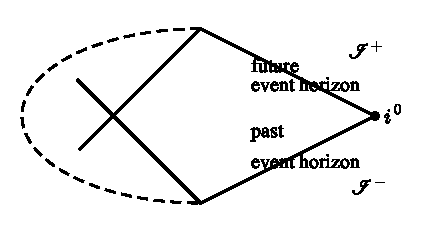
\includegraphics[width=0.72\textwidth]{fig_6.1.pdf}
\caption*{图 6.1\quad 渐近平直时空是指：其共形图中的无限远与 Minkowski 时空的无限远一致，包括未来类光无限远 $\mathscr{I}^{+}$、类空无限远 $i^{0}$ 和过去类光无限远 $\mathscr{I}^{-}$。未来事件视界是 $\mathscr{I}^{+}$ 的过去的边界。虚线区域代表时空的其余部分，在不同的例子中它可以呈现多种不同的形式。}
\end{figure}
正如第 5 章提到的，在无穷远处看起来像 Minkowski 时空的时空被称为渐近平直（asymptotically flat）时空。这个概念的含义在一幅诸如图 6.1 那样的共形图中一目了然。从附录 H 中关于 Minkowski 时空共形图的讨论我们知道，共形无限远分为五块：未来与过去类时无限远 $i^{\pm}$、未来与过去类光无限远 $\mathscr{I}^{\pm}$，以及类空无限远 $i^{0}$。如果一个时空（或时空的一个区域）的 $\mathscr{I}^{\pm}$ 和 $i^{0}$ 具有与 Minkowski 时空相同的结构，它就是渐近平直的；类时无限远则不是必需的。这样的时空一般具有图 6.1 所示的形态。

有了这幅图像，我们应该如何理解未来事件视界就清楚了：它是类时曲线无法再逃逸到无穷远的那一侧边界曲面。回忆一个区域的因果过去 $J^{-}$，是指从该区域出发、沿指向过去的类时路径所能到达的所有点的集合；事件视界于是可以等价地定义为 $J^{-}(\mathscr{I}^{+})$——即未来类光无限远的因果过去——的边界。（事件视界其实应当是这个集合的\emph{闭包}（closure）的边界，不过我们在这里不追求严格。）对过去视界也有类似的定义。正如在对 Schwarzschild 作最大延拓的情形中所看到的，一个时空中可以不止有一个渐近平直区域，相应地也就不止有一个事件视界。

从定义可以看出，事件视界是一个类光超曲面。类光超曲面的性质在附录 D 中讨论过；这里我们回顾一下其主要特点。一个超曲面 $\Sigma$ 可以由某个函数 $f(x)$ 通过 $f(x)=$ 常数来定义。梯度 $\partial_\mu f$ 与 $\Sigma$ 正交；若法矢量是类光的，就称这个超曲面为类光超曲面，此时法矢量同时也切于 $\Sigma$。类光超曲面可以看成是一族类光测地线 $x^{\mu}(\lambda)$ 的集合，这些测地线称为该超曲面的生成元（generators）。这些测地线的切矢量 $\xi^{\mu}$ 与法矢量成比例，

% ---- 书页 241 / p256 ----
\begin{equation*}
\xi^\mu = \frac{dx^\mu}{d\lambda} = h(x)g^{\mu\nu}\partial_\nu f,
\tag{6.1}
\end{equation*}
因而也可以充当超曲面的法矢量。我们可以选取函数 $h(x)$，使得这些测地线是仿射参量化的，于是切矢量将满足
\begin{equation*}
\xi_\mu\xi^\mu = 0, \qquad \xi^\mu\nabla_\mu\xi^\nu = 0.
\tag{6.2}
\end{equation*}
对于未来事件视界，其生成元可以在过去终结（例如，当黑洞由恒星坍缩形成时），但总会一直延伸到无穷远的未来（未来与过去互换后亦然）。

由于事件视界是一个整体性的概念，如果有人递给你一个用任意坐标写出的度规，要真正找到它的视界位置可能相当困难。幸运的是，本章我们要打交道的都是相当特殊的度规——稳态、渐近平直，而且含有拓扑为球面的事件视界。在这类时空中，存在一些方便的坐标系，使得辨认事件视界有一种简单办法。对 Schwarzschild 解来说，事件视界是光锥“倾倒”的地方，使得 $r=2GM$ 成为一个类光曲面，而不像在大 $r$ 处那样 $r=$ 常数是类时曲面。光锥倾倒显然是一个依赖坐标的概念（比如在 Kruskal 坐标中就不会发生），但我们关心的那些度规都容许类似的构造。稳态度规有一个渐近类时的 Killing 矢量 $\partial_t$，我们可以调整度规分量使之与时间无关（$\partial_t g_{\mu\nu}=0$）。在 $t=$ 常数的超曲面上，我们可以选取坐标 $(r,\theta,\phi)$，使得无穷远处的度规看起来就像球坐标下的 Minkowski 空间。$r=$ 常数的超曲面在 $r\to\infty$ 处将是拓扑为 $S^{2}\times\mathbf{R}$ 的类时柱面。现在设想我们聪明地选好了坐标，使得当 $r$ 从无穷远逐渐减小时，$r=$ 常数的超曲面始终保持类时，直到某个固定的 $r=r_{\mathrm{H}}$ 处，曲面处处类光。（在不那么聪明的坐标中，$r=$ 常数的超曲面会在某些 $\theta$ 和 $\phi$ 值处变成类光或类空，而在其他值处仍是类时。）这显然就代表一个事件视界，因为跨入 $r<r_{\mathrm{H}}$ 区域的类时路径永远无法逃回无穷远。确定 $r=$ 常数超曲面在何处变为类光很容易：$\partial_\mu r$ 是这种超曲面的一个法 1-形式，其模长为
\begin{equation*}
g^{\mu\nu}(\partial_\mu r)(\partial_\nu r) = g^{rr}.
\tag{6.3}
\end{equation*}
我们要找的正是这个 1-形式的模长为零的地方；于是，在我们所描述的坐标中，事件视界 $r=r_{\mathrm{H}}$ 就是 $g^{rr}$ 由正变负的那个超曲面，
\begin{equation*}
g^{rr}(r_{\mathrm{H}}) = 0.
\tag{6.4}
\end{equation*}

% ---- 书页 242 / p257 ----
这条判据对 Schwarzschild 解显然有效，因为它的 $g^{rr}=1-2GM/r$。后面我们给出 Reissner–Nordström 解和 Kerr 解时，也将采用类似地适配于视界的坐标。

我们之所以把事件视界看得如此重要，是因为在广义相对论中它们几乎是不可避免的。这一结论由两个有趣的结果串联而来：奇点几乎不可避免，而且奇点藏在事件视界背后。当然，两个结果都在各自的一组适当假设下才成立；构造没有奇点的时空并不难（Minkowski 空间就是一例），找到没有视界的奇点也不算难（下面讨论带电黑洞时就会看到）。但我们相信，“通有”（generic）的解都会有藏在视界背后的奇点。

奇点的普遍存在由 Hawking 和 Penrose 的\textbf{奇点定理}（singularity theorems）保证。在这些定理被证明之前，人们还可以指望，坍缩到 Schwarzschild 奇点只是球对称性的一个人为假象，典型的几何将保持无奇点（例如在 Newton 引力中就是这样）。但 Hawking–Penrose 定理表明，坍缩一旦达到某个程度，向奇点的演化就不可避免。我们知道存在奇点的途径是测地不完备（geodesic incompleteness）——存在某条测地线，它无法在流形内延伸，却在仿射参量的有限值处终结。而我们知道坍缩已经达到有去无回之点的标志，是一个\textbf{陷俘面}（trapped surface）的出现。要理解什么是陷俘面，先想象 Minkowski 空间中的一个二维球面，它嵌在一个等时切片里，取为到原点径向距离固定的一些点。如果我们追踪从这个空间球面射向时空的类光线，一族（指向内部）将描绘出一组不断收缩的球面，而另一族（指向外部）将描绘出一组不断胀大的球面。但对 Schwarzschild 几何中半径固定为 $r<2GM$ 的球面来说，情况就不是这样了；在事件视界之内，从这个球面发出的两组类光线都会演化到更小的 $r$ 值（因为 $r$ 是类时坐标），从而演化到更小的面积 $4\pi r^{2}$。这就是陷俘面的含义：一个紧致、类空的二维子流形，其性质是在该子流形上处处，指向未来的出射光线沿两个方向都\emph{汇聚}。（“汇聚”的正式定义是：膨胀 $\theta$——正如附录 F 中关于测地线汇的讨论所描述的——为负。）

有了这些定义，我们就可以给出一个奇点定理的例子。

令 $M$ 是一个流形，带有通有的度规 $g_{\mu\nu}$，满足 Einstein 方程并施加强能量条件。如果 $M$ 中存在一个陷俘面，则必定要么存在一条闭合类时曲线，要么存在一个奇点（表现为某条不完备的类时或类光测地线）。

% ---- 书页 243 / p258 ----
这里所谓“通有度规”，指的是对类时和类光测地线都满足\textbf{普适条件}（generic condition）。对类时测地线，普适条件是说：每条以 $U^{\mu}$ 为切矢量的测地线，都必须至少有一个点使得 $R_{\alpha\beta\gamma\delta}U^{\alpha}U^{\delta}\neq 0$；对类光测地线，普适条件是说：每条以 $k^{\mu}$ 为切矢量的测地线，都必须至少有一个点使得 $k_{[\alpha}R_{\beta]\gamma\delta[\epsilon}k_{\xi]}k^{\gamma}k^{\delta}\neq 0$。这些花哨的条件不过是用来排除那些曲率在某些方向上一致为零的特殊度规。

奇点定理有许多种形式，各自从不同的一组假设出发。这个故事的寓意似乎是：广义相对论中典型的含时解通常终于奇点。（或者始于奇点；某些定理暗示了宇宙学奇点的存在，比如大爆炸。）这对 GR 来说算是个问题，因为这个理论其实并不真正适用于奇点本身，奇点的存在因此代表着描述的不完备性。对待这个问题的传统态度，是寄希望于众人苦苦追寻的量子引力理论，能以某种方式化解经典 GR 的奇点。

与此同时，我们还可以从“奇点藏在事件视界背后”这一想法中获得安慰。这一信念概括在\textbf{宇宙监督假设}（cosmic censorship conjecture）之中：

在满足主能量条件的渐近平直时空中，从通有的、初始非奇异的态出发的引力坍缩，不能形成裸奇点。

\textbf{裸奇点}（naked singularity）是指信号可以从那里到达 $\mathscr{I}^{+}$ 的奇点；也就是说，是没有藏在事件视界背后的奇点。注意，这个假设讲的是裸奇点的\emph{形成}，而不是它们的\emph{存在}；当然有一些解，其类空裸奇点存在于过去（比如 Schwarzschild 白洞），或者类时奇点存在于所有时间（比如下面要讨论的超极端带电黑洞）。宇宙监督假设至今未被证明，尽管人们已经花了大量力气去寻找有说服力的反例，却一无所获。要求初始数据在某种意义上“通有”这一点很重要，因为数值实验表明，经过精细调节的初始条件能够产生裸奇点。对某种形式的宇宙监督假设给出严格证明，仍然是经典广义相对论悬而未决的突出问题之一。\footnote{关于宇宙监督假设的评述见 R.M. Wald, “Gravitational Collapse and Cosmic Censorship,” http://arxiv.org/abs/gr-qc/9710068.}

宇宙监督（或某些等价假设）的一个推论是：经典黑洞从不缩小，只会越长越大。黑洞的大小由事件视界的面积来量度，这里指的是事件视界与一个类空切片之交的空间面积。于是我们有了 Hawking 的\textbf{面积定理}（area theorem）：

假设弱能量条件与宇宙监督成立，则渐近平直时空中未来事件视界的面积不减。

% ---- 书页 244 / p259 ----
对 Schwarzschild 黑洞，面积单调地依赖于质量，因此这个定理意味着 Schwarzschild 黑洞的质量只能增加。但对转动的黑洞就不再如此了；面积依赖于质量和角动量的某种组合，而且下面我们会看到，通过减小黑洞的自旋，我们真的可以从中提取能量。我们也可以通过量子力学的霍金辐射来减小黑洞的质量；这可以追溯到弯曲时空中的量子场论可以违反弱能量条件这一事实。

\section{Killing 视界}

在 Schwarzschild 度规中，Killing 矢量 $K=\partial_t$ 在事件视界处由类时变为类空。一般地，如果某个 Killing 矢量场 $\chi^{\mu}$ 沿某个类光超曲面 $\Sigma$ 处处类光，我们就说 $\Sigma$ 是 $\chi^{\mu}$ 的一个\textbf{Killing 视界}（Killing horizon）。注意矢量场 $\chi^{\mu}$ 必然与 $\Sigma$ 正交，因为一个类光曲面不可能有两个线性无关的类光切矢量。

Killing 视界的概念在逻辑上独立于事件视界的概念，但在具有时间平移对称性的时空中，两者紧密相关。在某些合理的条件下（下面会明确给出），我们有如下分类：

稳态、渐近平直时空中的每一个事件视界 $\Sigma$，都是某个 Killing 矢量场 $\chi^{\mu}$ 的 Killing 视界。

如果时空是静态的，$\chi^{\mu}$ 就是代表无穷远处时间平移的 Killing 矢量场 $K^{\mu}=(\partial_t)^{\mu}$。

如果时空是稳态但非静态的，它将是轴对称的，并带有转动 Killing 矢量场 $R^{\mu}=(\partial_\phi)^{\mu}$，而 $\chi^{\mu}$ 将是线性组合 $K^{\mu}+\Omega_{\mathrm{H}}R^{\mu}$，其中 $\Omega_{\mathrm{H}}$ 为某个常数。

例如，下面我们将考察转动黑洞的 Kerr 度规，其中事件视界是转动与时间平移的 Killing 矢量的某个线性组合的 Killing 视界。在 Kerr 情形，$\partial_t$ 变为类光的那个超曲面实际上是类时的，因此并不是 Killing 视界。

让我们把这套分类方案究竟在什么条件下成立说得更精确些。\footnote{相关讨论见 R. M. Wald, “The thermodynamics of black holes,” \emph{Living Rev.\ Rel.} \textbf{4}, 6 (2001), http://arxiv.org/gr-qc/9912119.}Carter 已经证明，对静态黑洞，事件视界是 $K^{\mu}$ 的 Killing 视界；这是一个纯几何的事实，即使不引用 Einstein 方程也成立。在稳态情形，如果我们假设存在一个转动 Killing 场 $R^{\mu}$，它具有这样的性质：由 $K^{\mu}$ 和 $R^{\mu}$ 张成的二维平面与一族二维曲面正交，那么事件视界将是这两个 Killing 场的某个线性组合的 Killing 视界——这同样是纯几何的论证。反过来，如果我们只假设黑洞是稳态的，那么一般说来我们无法证明事件视界
% ---- 书页 245 / p260 ----
是轴对称的。给定 Einstein 方程加上对物质场的某些条件，Hawking 得以证明：任何稳态黑洞的事件视界必定是某个矢量场的 Killing 视界，而且这类视界必定要么稳态、要么轴对称。在本章剩下的部分里，我们将当作上述分类成立那样来叙述；然而，对物质场作假设是出了名的棘手，我们应当记住，原则上有可能找到既非静态也非轴对称的黑洞，对它们来说事件视界可能就不是 Killing 视界。

需要着重指出的一点是：虽然稳态渐近平直时空的事件视界通常是 Killing 视界，但也很容易找到与事件视界毫不相干的 Killing 视界。考虑用惯性坐标表示的 Minkowski 空间，$\mathrm{d}s^{2}=-\mathrm{d}t^{2}+\mathrm{d}x^{2}+\mathrm{d}y^{2}+\mathrm{d}z^{2}$；显然这个时空中没有任何事件视界。生成 $x$ 方向推动（boost）的 Killing 矢量为
\begin{equation*}
\chi = x\partial_t + t\partial_x,
\tag{6.5}
\end{equation*}
其模长为
\begin{equation*}
\chi_\mu\chi^\mu = -x^{2} + t^{2}.
\tag{6.6}
\end{equation*}
它在类光曲面
\begin{equation*}
x = \pm t,
\tag{6.7}
\end{equation*}
上变为类光，因此这些曲面就是 Killing 视界。把推动 Killing 矢量与平移和转动 Killing 矢量组合起来，我们就能让这些视界在流形中到处移动；Killing 视界俯拾皆是。当然，在更有意思的时空中，Killing 矢量场要少一些，相应的视界（如果有的话）也会有更大的物理意义。

对每一个 Killing 视界，我们都可以关联一个叫做\textbf{表面引力}（surface gravity）的量。考虑一个带有 Killing 视界 $\Sigma$ 的 Killing 矢量 $\chi^{\mu}$。因为 $\chi^{\mu}$ 是 $\Sigma$ 的法矢量，沿着 Killing 视界它满足测地线方程，
\begin{equation*}
\chi^\mu\nabla_\mu\chi^\nu = -\kappa\chi^\nu,
\tag{6.8}
\end{equation*}
等号右边的出现是因为 $\chi^{\mu}$ 的积分曲线未必是仿射参量化的。参量 $\kappa$ 就是表面引力；它在视界上为常数，除非在 Killing 矢量为零、$\kappa$ 可以变号的“分岔二维球面”（bifurcation two-sphere）处。（例如，在 Schwarzschild 解的 Kruskal 图中心就会发生这种情况。）利用 Killing 方程 $\nabla_{(\mu}\chi_{\nu)}=0$ 以及 $\chi_{[\mu}\nabla_\nu\chi_{\sigma]}=0$ 这一事实（因为 $\chi^{\mu}$ 与 $\Sigma$ 正交），可以直截了当地导出一个漂亮的表面引力公式：
\begin{equation*}
\kappa^{2} = -\frac{1}{2}(\nabla_\mu\chi_\nu)(\nabla^\mu\chi^\nu).
\tag{6.9}
\end{equation*}
右边的表达式要在视界 $\Sigma$ 上取值。鼓励你自己动手验证一下这个公式。

% ---- 书页 246 / p261 ----
与 Killing 视界相联系的表面引力原则上带有任意性，因为我们总可以用一个实常数去缩放某个 Killing 场而得到另一个 Killing 场。在静态、渐近平直的时空中，时间平移 Killing 矢量 $K=\partial_t$ 可以通过令
\begin{equation*}
K_\mu K^\mu(r\to\infty) = -1
\tag{6.10}
\end{equation*}
来归一化。这又随之确定了任何相关联的 Killing 视界的表面引力。如果我们处在稳态时空中，那里的 Killing 视界与时间平移和转动的某个线性组合相联系，那么固定 $K=\partial_t$ 的归一化也就固定了这个线性组合，因此表面引力仍然是唯一的。

$\kappa$ 为什么叫做“表面引力”，只有当时空是静态的时候才变得清楚。在这种情形下我们有如下解释：

在静态、渐近平直的时空中，表面引力就是视界附近一位静态观者的加速度，由无穷远处的一位静态观者测得。

为了弄清这句话的含义，我们先来考虑静态观者。所谓静态观者，指的是其四速度 $U^{\mu}$ 与时间平移 Killing 场 $K^{\mu}$ 成正比的观者，
\begin{equation*}
K^\mu = V(x)U^\mu.
\tag{6.11}
\end{equation*}
由于四速度归一化为 $U_\mu U^{\mu}=-1$，函数 $V$ 不过就是 Killing 场的模长，
\begin{equation*}
V = \sqrt{-K_\mu K^\mu},
\tag{6.12}
\end{equation*}
因而从 Killing 视界处的零一直取到无穷远处的 1。$V$ 有时被称为“红移因子”（redshift factor），因为它把静态观者所测得的一个光子的发射频率与观测频率联系起来。回忆一下，四动量为 $p^{\mu}$ 的光子的守恒能量是 $E=-p_\mu K^{\mu}$，而由四速度为 $U^{\mu}$ 的观者测得的频率将是 $\omega=-p_\mu U^{\mu}$。因此
\begin{equation*}
\omega = \frac{E}{V},
\tag{6.13}
\end{equation*}
而静态观者 1 发射的一个光子将被静态观者 2 观测到具有波长 $\lambda=2\pi/\omega$，
\begin{equation*}
\lambda_2 = \frac{V_2}{V_1}\lambda_1.
\tag{6.14}
\end{equation*}
特别地，在 $V=1$ 的无穷远处，我们将观测到波长 $\lambda_{\infty}=\lambda_{1}/V_{1}$。

现在我们转向“从无穷远处看到的加速度”这个概念。静态观者一般不会沿测地线运动；比如，粒子往往要落进黑洞，而不是悬停在黑洞旁边、保持空间坐标固定。

% ---- 书页 247 / p262 ----
我们可以把四加速度 $a^{\mu}=U^{\sigma}\nabla_{\sigma}U^{\mu}$ 用红移因子表示为
\begin{equation*}
a_\mu = \nabla_\mu\ln V,
\tag{6.15}
\end{equation*}
这一点你很容易验证。加速度的大小
\begin{equation*}
a = \sqrt{a_\mu a^\mu} = V^{-1}\sqrt{\nabla_\mu V\nabla^\mu V},
\tag{6.16}
\end{equation*}
在 Killing 视界处将趋于无穷——要让一个物体保持在静态轨迹上，需要无穷大的加速度。但无穷远处的观者探测到的加速度将被因子 $V$“红移”；这个结果正是表面引力。于是我们断言，
\begin{equation*}
\kappa = Va = \sqrt{\nabla_\mu V\nabla^\mu V},
\tag{6.17}
\end{equation*}
在视界 $\Sigma$ 上取值。你可以验证这个表达式与式 (6.9) 一致。表面引力是零（$V$）与无穷（$a$）的乘积，但通常取有限值。当我们说观测到的加速度被红移了，我们脑海中的图像是：把一根检验细绳从一个位于视界处的静态物体一直拉伸到无穷远处的观者，然后测量细绳在无穷远那一端的加速度。（值得花点时间看看，你能否把这个挥手带过的论证提升为某种更严格的东西。）

如果时空是稳态但非静态的，上面的考虑会在哪里出问题？我们仍然有一个渐近的时间平移 Killing 矢量 $K=\partial_t$，而且可以像式 (6.11) 那样，把四速度与 $K^{\mu}$ 平行的观者定义为稳态观者；红移仍由式 (6.14) 给出。问题在于，$K^{\mu}$ 不会在 Killing 视界处变为类光，而一般是在视界之外某个类时曲面上变为类光。这个 $K^{\mu}K_\mu=0$ 的地方被称为\textbf{静止极限面}（stationary limit surface）（有时也称“能层面”（ergosurface）），因为在这个曲面之内 $K^{\mu}$ 是类空的，因而任何观者都无法保持静止，哪怕这里还在事件视界之外。这样的观者不得不相对于 Killing 场运动，但不必朝着黑洞的方向运动。由式 (6.12) 和式 (6.14)，当我们趋近静止极限面时，稳态观者的红移发散，因此这个曲面也被称为\textbf{无限红移面}（infinite redshift surface）。正如我们在讨论 Kerr 度规时将会看到的，静止极限面与事件视界之间的区域——能层（ergosphere）——是一个类时路径不可避免地被拖着随黑洞一起转动的地方。在稳态时空中我们将继续使用“表面引力”这个标签，并用 Killing 矢量 $\chi^{\mu}$（它在事件视界上确实变为类光）来计算它，即使所得的量已不能解释为无穷远处所看到的静态观者的引力加速度。

让我们把这些概念应用到 Schwarzschild 情形，看看它们如何运作。对于度规
\begin{equation*}
\mathrm{d}s^{2} = -\left(1-\frac{2GM}{r}\right)\mathrm{d}t^{2} + \left(1-\frac{2GM}{r}\right)^{-1}\mathrm{d}r^{2} + r^{2}\,\mathrm{d}\Omega^{2},
\tag{6.18}
\end{equation*}

% ---- 书页 248 / p263 ----
Killing 矢量和静态四速度为
\begin{equation*}
K^\mu = (1,\ 0,\ 0,\ 0), \qquad U^\mu = \left[\left(1-\frac{2GM}{r}\right)^{-1/2},\ 0,\ 0,\ 0\right],
\tag{6.19}
\end{equation*}
于是红移因子为
\begin{equation*}
V = \sqrt{1-\frac{2GM}{r}}.
\tag{6.20}
\end{equation*}
（注意这与上一章中我们对红移的计算相符。）由式 (6.15)，加速度为
\begin{equation*}
a_\mu = \frac{GM}{r^{2}\left(1-\dfrac{2GM}{r}\right)}\nabla_\mu r,
\tag{6.21}
\end{equation*}
其中当然有 $\nabla_\mu r=\delta^{r}_{\mu}$。于是加速度的大小为
\begin{equation*}
a = \frac{GM}{r^{2}\left(1-\dfrac{2GM}{r}\right)^{1/2}}.
\tag{6.22}
\end{equation*}
表面引力是 $\kappa=Va$ 在事件视界 $r=2GM$ 处的取值，而
\begin{equation*}
Va = \frac{GM}{r^{2}},
\tag{6.23}
\end{equation*}
所以 Schwarzschild 黑洞的表面引力为
\begin{equation*}
\kappa = \frac{1}{4GM}.
\tag{6.24}
\end{equation*}
表面引力随质量增大反而减小，这看上去也许令人诧异，但只要看一眼式 (6.23) 就明白是怎么回事了：在固定半径处，增大 $M$ 确实会使组合 $Va$ 变大，但质量的增大同时也使 Schwarzschild 半径增大，后一种效应占了上风。因此，大黑洞的表面引力实际上比小黑洞的还要弱；这与对潮汐力的考察相一致——黑洞越大，潮汐力也越小。

\section{质量、电荷与自旋}

我们在上面曾宣称，广义相对论最一般的稳态黑洞解由质量、电荷和自旋刻画，那么就应该考虑这些量在 GR 中如何定义。电荷最容易考虑，所以我们从它开始；更多细节见附录 E 中关于 Stokes 定理的讨论。我们将具体考察电荷，不过磁荷也可以用同样的方式来处理。

% ---- 书页 249 / p264 ----
麦克斯韦方程组把电磁场强张量 $F_{\mu\nu}$ 与电流四矢量 $J^{\mu}_{e}$ 联系起来，
\begin{equation*}
\nabla_\nu F^{\mu\nu} = J^{\mu}_{e}.
\tag{6.25}
\end{equation*}
穿过类空超曲面 $\Sigma$ 的电荷由该超曲面上坐标 $x^{i}$ 的积分给出，
\begin{align*}
Q &= -\int_{\Sigma} d^{3}x\,\sqrt{\gamma}\, n_\mu J^{\mu}_{e}\\
  &= -\int_{\Sigma} d^{3}x\,\sqrt{\gamma}\, n_\mu\nabla_\nu F^{\mu\nu},
\tag{6.26}
\end{align*}
其中 $\gamma_{ij}$ 是与 $\Sigma$ 相联系的诱导度规，$n^{\mu}$ 是单位法矢量。这个负号保证正的电荷密度加上指向未来的法矢量会给出正的总电荷。于是可以用 Stokes 定理把电荷表示成一个边界积分，
\begin{equation*}
Q = -\int_{\partial\Sigma} d^{2}x\,\sqrt{\gamma^{(2)}}\, n_\mu\sigma_\nu F^{\mu\nu},
\tag{6.27}
\end{equation*}
其中边界 $\partial\Sigma$——典型地是空间无穷远处的一个二维球面——具有度规 $\gamma^{(2)}_{ij}$ 和指向外部的法矢量 $\sigma^{\mu}$。磁荷则可以通过把 $F^{\mu\nu}$ 换成对偶张量 ${*F}^{\mu\nu}=\frac{1}{2}\epsilon^{\mu\nu\rho\sigma}F_{\rho\sigma}$ 来确定。因此，要计算总电荷，我们只需要知道电磁场在空间无穷远处的行为。在附录 E 中，我们对 Minkowski 空间中的一个点电荷作了显式计算，得到的结果不出所料，但很好地检验了我们的约定确实自洽。

现在我们转向渐近平直时空的总能量（或质量）的概念。这是一个比电荷棘手得多的概念；一方面，在广义相对论中能量-动量是张量而不是矢量；另一方面，能量-动量张量 $T_{\mu\nu}$ 只描述物质的性质，而不描述引力场的性质。但回忆一下，第 3 章中我们讨论过：如果时空是稳态的、具有类时 Killing 矢量场 $K^{\mu}$，我们仍然可以定义一个守恒的总能量。我们先构造一个流
\begin{equation*}
J^{\mu}_{T} = K_\nu T^{\mu\nu},
\tag{6.28}
\end{equation*}
其中 $T^{\mu\nu}$ 是能量-动量张量。因为这个流是无散的（由 Killing 方程和 $T^{\mu\nu}$ 的守恒而来），我们可以在一个类空曲面 $\Sigma$ 上积分，得到一个守恒的能量，
\begin{equation*}
E_{T} = \int_{\Sigma} d^{3}x\,\sqrt{\gamma}\, n_\mu J^{\mu}_{T},
\tag{6.29}
\end{equation*}
就像电荷那样。这个表达式虽然有趣，但显然有几点不足。例如考虑 Schwarzschild 度规，它有一个
% ---- 书页 250 / p265 ----
Killing 矢量，但 $T^{\mu\nu}$ 处处为零。那么 Schwarzschild 黑洞的能量就是零吗？无论从物理还是数学的理由看，都有理由怀疑并非如此；毕竟那里有一个奇点，它使得这个积分很难算出来。此外，Schwarzschild 黑洞可以由一颗具有确定非零能量的大质量恒星演化而来，我们或许愿意让这个能量守恒。因此值得去寻找另一种能量定义，以便更好地捕捉我们对黑洞时空的直观图像。

我们暂时仍然限于具有类时 Killing 矢量 $K^{\mu}$ 的时空，考虑一个新的流
\begin{equation*}
J^{\mu}_{R} = K_\nu R^{\mu\nu}.
\tag{6.30}
\end{equation*}
利用 Einstein 方程，我们也可以把它等价地写成
\begin{equation*}
J^{\mu}_{R} = 8\pi G K_\nu\left(T^{\mu\nu}-\frac{1}{2}T g^{\mu\nu}\right).
\tag{6.31}
\end{equation*}
Ricci 张量并不是无散的；我们有的是缩并的 Bianchi 恒等式，
\begin{equation*}
\nabla_\mu R^{\mu\nu} = \frac{1}{2}\nabla^{\nu}R.
\tag{6.32}
\end{equation*}
但这个恒等式加上 Killing 方程，就足以保证我们的新流是守恒的。为看清这一点，我们只需计算
\begin{equation*}
\nabla_\mu J^{\mu}_{R} = (\nabla_\mu K_\nu)R^{\mu\nu} + K_\nu(\nabla_\mu R^{\mu\nu}).
\tag{6.33}
\end{equation*}
第一项为零，因为 $R^{\mu\nu}$ 是对称的，而 $\nabla_\mu K_\nu$ 是反对称的（由 Killing 方程）。于是利用式 (6.32)，我们得到
\begin{equation*}
\nabla_\mu J^{\mu}_{R} = \frac{1}{2}K_\nu\nabla^{\nu}R = 0,
\tag{6.34}
\end{equation*}
我们知道它为零，因为 $R$ 沿 Killing 矢量的方向导数为零，见式 (3.178)。

和前面一样，我们可以定义一个与这个流相联系的守恒能量，
\begin{equation*}
E_{R} = \frac{1}{4\pi G}\int_{\Sigma} d^{3}x\,\sqrt{\gamma}\, n_\mu J^{\mu}_{R},
\tag{6.35}
\end{equation*}
其中归一化的选取是为了将来的方便。能量 $E_{R}$ 将不依赖于类空超曲面 $\Sigma$ 的选取，因而是守恒的。这个能量概念比起 $E_{T}$ 有一项显著的优势，源于这样一个事实：$E_{R}$ 可以改写成空间无穷远处一个二维球面上的面积分。为看清这一点，回忆式 (3.177)：任何 Killing 矢量都满足 $\nabla_\mu\nabla_\nu K^{\mu}=K^{\mu}R_{\mu\nu}$；于是这个流本身可以写成一个全导数，
\begin{equation*}
J^{\mu}_{R} = \nabla_\nu(\nabla^{\mu}K^{\nu}),
\tag{6.36}
\end{equation*}
 于是有
% ---- 书页 251 / p266 ----
\begin{equation*}
E_{R} = \frac{1}{4\pi G}\int_{\Sigma} d^{3}x\,\sqrt{\gamma}\, n_{\mu}\nabla_{\nu}\left(\nabla^{\mu}K^{\nu}\right).
\tag{6.37}
\end{equation*}

注意，由 Killing 方程升起指标可得 $\nabla^{\mu}K^{\nu}=-\nabla^{\nu}K^{\mu}$。因此，正如前面处理电荷时那样，我们可以再次利用 Stokes 定理，把 $E_{R}$ 写成空间无穷远处的积分，
\begin{equation*}
\boxed{\,E_{R} = \frac{1}{4\pi G}\int_{\partial\Sigma} d^{2}x\,\sqrt{\gamma^{(2)}}\, n_{\mu}\sigma_{\nu}\nabla^{\mu}K^{\nu}.\,}
\tag{6.38}
\end{equation*}
这个表达式就是与类时 Killing 矢量 $K^{\mu}$ 相联系的\textbf{Komar 积分}（Komar integral）；它可以解释为稳态时空的总能量。

为了让我们自己确信方向没错，就用度规为式 (6.18) 的 Schwarzschild 时空来算一算 Komar 积分。归一化为 $n_{\mu}n^{\mu}=-1$ 与 $\sigma_{\mu}\sigma^{\mu}=+1$ 的法矢量，其非零分量为
\begin{equation*}
n_{0} = -\left(1-\frac{2GM}{r}\right)^{1/2}, \qquad \sigma_{1} = \left(1-\frac{2GM}{r}\right)^{-1/2},
\tag{6.39}
\end{equation*}
其余分量均为零。于是我们有
\begin{equation*}
n_{\mu}\sigma_{\nu}\nabla^{\mu}K^{\nu} = -\nabla^{0}K^{1}.
\tag{6.40}
\end{equation*}
Killing 矢量为 $K^{\mu}=(1,0,0,0)$，因此我们可以毫不费力地算出
\begin{align*}
\nabla^{0}K^{1} &= g^{00}\nabla_{0}K^{1}\\
&= g^{00}\left(\partial_{0}K^{1}+\Gamma^{1}_{0\lambda}K^{\lambda}\right)\\
&= g^{00}\Gamma^{1}_{00}K^{0}\\
&= -\left(1-\frac{2GM}{r}\right)^{-1}\frac{GM}{r^{2}}\left(1-\frac{2GM}{r}\right)\\
&= -\frac{GM}{r^{2}}.
\tag{6.41}
\end{align*}
无穷远处二维球面上的度规是
\begin{equation*}
\gamma^{(2)}_{ij}\,\mathrm{d}x^{i}\mathrm{d}x^{j} = r^{2}\left(\mathrm{d}\theta^{2}+\sin^{2}\theta\,\mathrm{d}\phi^{2}\right),
\tag{6.42}
\end{equation*}
于是
\begin{equation*}
\sqrt{\gamma^{(2)}} = r^{2}\sin\theta.
\tag{6.43}
\end{equation*}

% ---- 书页 252 / p267 ----
把这一切合在一起，Schwarzschild 黑洞的能量就是
\begin{align*}
E_{R} &= \frac{1}{4\pi G}\int d\theta\, d\phi\, r^{2}\sin\theta\left(\frac{GM}{r^{2}}\right)\\
&= M.
\tag{6.44}
\end{align*}
这当然正是我们想要的结果，同时也解释了式 (6.35) 中所选取的归一化。

尽管得到了正确的答案，我们还是应该想一想刚才到底发生了什么。具体来说，我们是把流 $J^{\mu}_{R}=K_{\nu}R^{\mu\nu}$ 在一个类空切片上积分而得到这个能量的，并且发现结果可以写成空间无穷远处的积分。但对 Schwarzschild 来说，度规满足真空 Einstein 方程 $R_{\mu\nu}=0$；这样一来，要从对 $J^{\mu}_{R}$ 的积分中得到非零的结果似乎就很困难，正如式 (6.29) 那样。可是如果想一想最大延拓 Schwarzschild 解的结构，我们就会意识到，可以画出两类类空切片：一类穿过虫洞一直延伸到第二个渐近区域，另一类则终止于奇点。如果切片穿过虫洞，另一个渐近区域就会为 $\partial\Sigma$ 提供另一个组成部分，从而对式 (6.38) 提供另一份贡献；这份贡献会恰好抵消，于是总能量确实会是零。如果切片撞上了奇点，我们就不知道该怎么处理了。尽管如此，无论哪种情形，把我们的结果 (6.44) 当作正确的答案都是合理的。关键在于，式 (6.38) 只涉及空间无穷远处的贡献，所以无论内部发生什么，它都应当是能量的一个有效表达式。我们甚至可以设想内部出现随时间变化的行为；只要 $K^{\mu}$ \emph{渐近地}是类时 Killing 矢量，Komar 能量就是良定义的。比如说，我们可以考虑从一颗初始静态的恒星出发的球对称引力坍缩。直接在 $\Sigma$ 上计算积分 (6.35)，会给出一个合理的总质量答案，而且当恒星坍缩为黑洞时，这个总质量不应改变（我们设想的是球对称，因此引力辐射无法把能量带到无穷远）。于是，在坍缩之前有效的 Komar 积分 (6.38)，在坍缩成黑洞之后也尽可以放心地解释为能量。当然，出于某些目的，我们或许想容许通过引力辐射损失能量，那种情形下就必须小心对待如何把切片延伸到无穷远；人们可以在未来类光无限远处定义一个“Bondi 质量”（Bondi mass），用它来追踪通过辐射损失的能量。

关于 Komar 公式的另一个疑虑是，它是否真的是我们应当认作“能量”的那种东西——能量通常是指与时间平移不变性相联系的守恒量。支持这种解释的最好理由很简单：$E_{R}$ 无疑是某种守恒量，而且它与我们认为应当是 Schwarzschild 能量的数值相一致（在 Newton 极限下对一团质量合集也是如此，你可以自行验证），那么它还能是什么呢？另一种做法是考虑广义相对论的哈密顿表述，在渐近平直时空中仔细定义时间平移的生成元，再把它认同为总能量。这项工作最先由 Arnowitt、Deser 和 Misner 完成，他们的结果就是所谓的\textbf{ADM 能量}（ADM energy）。在一个
% ---- 书页 253 / p268 ----
渐近平直时空中，我们可以像在微扰论中那样把度规写成
\begin{equation*}
g_{\mu\nu} = \eta_{\mu\nu} + h_{\mu\nu},
\tag{6.45}
\end{equation*}
只不过这里我们只要求分量 $h_{\mu\nu}$ 在空间无穷远处很小，而不必处处都小。于是 ADM 能量可以写成空间无穷远处一个二维球面上的积分：
\begin{equation*}
E_{\mathrm{ADM}} = \frac{1}{16\pi G}\int_{\partial\Sigma} d^{2}x\,\sqrt{\gamma^{(2)}}\,\sigma^{i}\left(\partial_{j}h^{j}{}_{i}-\partial_{i}h^{j}{}_{j}\right),
\tag{6.46}
\end{equation*}
其中空间指标用 $\delta^{ij}$（无穷远处的空间度规）升起。这个公式看上去依赖于坐标的选取，但在我们的假设之下实际上是良定义的。如果 $h_{\mu\nu}$ 在无穷远处不依赖于时间，可以验证 ADM 能量与 Komar 能量实际上是一致的。这让我们更加相信 Komar 积分确实表示能量。不过，在某种意义上 ADM 能量更为“体面”；例如，如果存在与引力非最小耦合的长程标量场，Komar 积分就可能遇到麻烦。但就我们眼前的目的而言，Komar 能量已经完全够用了。

我们希望某个被叫作“能量”的东西具有这样一种品质：对任何物理位形它都是正的；否则，一个零能量的态就可以衰变成一些正能量的碎片和一些负能量的碎片。第 4 章讨论过的能量条件为物质场给出了正能量的概念，但我们可能会担心，引力的负能量贡献会带来麻烦。所幸在 GR 中我们有\textbf{正能量定理}（positive energy theorem），它最先由 Schoen 和 Yau（译注：原文排印作 “Shoen”，应为 Schoen。）证明：

无奇点的、满足 Einstein 方程和主能量条件的渐近平直时空，其 ADM 能量是非负的。而且，Minkowski 时空是唯一使 ADM 能量为零的此类时空。

如果容许奇点存在，反例显然是有的，比如 $M<0$ 的 Schwarzschild 解。不过，如果一个带奇点的时空（比如 $M>0$ 的 Schwarzschild 解）是作为无奇点初数据的演化结果而达到的，定理就仍然适用。这样看来，在广义相对论中我们似乎是安全的，不会遇到负能量的孤立系统。

最后，我们可以转向自旋（角动量）；讨论完能量之后，这一步轻而易举。设想我们有一个转动 Killing 矢量 $R=\partial_{\phi}$。与时间平移的情形完全类似，我们可以定义一个守恒流
\begin{equation*}
J^{\mu}_{\phi} = R_{\nu}R^{\mu\nu},
\tag{6.47}
\end{equation*}
由它将得到把守恒角动量 $J$ 表示成空间无穷远处积分的表达式，

% ---- 书页 254 / p269 ----
\begin{equation*}
\boxed{\,J = -\frac{1}{8\pi G}\int_{\partial\Sigma} d^{2}x\,\sqrt{\gamma^{(2)}}\, n_{\mu}\sigma_{\nu}\nabla^{\mu}R^{\nu}.\,}
\tag{6.48}
\end{equation*}
（“J”既被用来表示流又被用来表示角动量，“R”既是转动 Killing 矢量又是 Ricci 张量，这都挺遗憾。可是字母就只有这么多，只能将就了。）与能量一样，即使 $R^{\mu}$ 只是渐近地才是 Killing 矢量，这个表达式仍然有效。注意，这里的归一化与能量积分中的不同；例如，可以通过对弱引力场中缓慢运动的物体求出该表达式的值，来为这个归一化提供依据。

\section{带电（Reissner–Nordström）黑洞}

现在我们转向表示带电黑洞的精确解。这类解与现实的天体物理情形关系并不太大；在真实世界中，一个高电荷黑洞会通过与黑洞附近物质的相互作用迅速被中和。不过，带电黑洞仍然展示了更一般情形的若干重要特征。在这个问题中，完整的球对称性依然存在；因此我们知道可以把度规写成
\begin{equation*}
\mathrm{d}s^{2} = -e^{2\alpha(r,t)}\mathrm{d}t^{2} + e^{2\beta(r,t)}\mathrm{d}r^{2} + r^{2}\mathrm{d}\Omega^{2}.
\tag{6.49}
\end{equation*}
然而现在我们不再处于真空，因为黑洞会带有非零的电磁场，而电磁场又充当能量-动量的源。电磁场的能量-动量张量为
\begin{equation*}
T_{\mu\nu} = F_{\mu\rho}F_{\nu}{}^{\rho} - \frac{1}{4}g_{\mu\nu}F_{\rho\sigma}F^{\rho\sigma},
\tag{6.50}
\end{equation*}
其中 $F_{\mu\nu}$ 是电磁场强张量。既然问题具有球对称性，最一般的场强张量就只能有如下分量
\begin{gather*}
F_{tr} = f(r,t) = -F_{rt}\\
F_{\theta\phi} = g(r,t)\sin\theta = -F_{\phi\theta},
\tag{6.51}
\end{gather*}
其中 $f(r,t)$ 和 $g(r,t)$ 是两个有待场方程确定的函数，没有写出的分量均为零。$F_{tr}$ 对应于径向电场，而 $F_{\theta\phi}$ 对应于径向磁场。如果你正纳闷那个 $\sin\theta$ 是从哪儿来的，回忆一下：不应当依赖于 $\theta$ 和 $\phi$ 的量，是磁场的径向分量 $B^{r}=\epsilon^{01\mu\nu}F_{\mu\nu}$。对球对称的度规，
\begin{equation*}
\epsilon^{\rho\sigma\mu\nu} = \frac{1}{\sqrt{-g}}\tilde{\epsilon}^{\rho\sigma\mu\nu}
\end{equation*}
与 $(\sin\theta)^{-1}$ 成正比，所以我们希望在 $F_{\theta\phi}$ 中带有一个 $\sin\theta$ 因子。

% ---- 书页 255 / p270 ----
这种情形下的场方程既有 Einstein 方程，也有麦克斯韦方程组：
\begin{gather*}
g^{\mu\nu}\nabla_{\mu}F_{\nu\sigma} = 0\\
\nabla_{[\mu}F_{\nu\rho]} = 0.
\tag{6.52}
\end{gather*}
这两组方程彼此耦合在一起，因为电磁场强张量通过能量-动量张量进入 Einstein 方程，而度规又显式地出现在麦克斯韦方程组之中。

然而，这些困难并非不可克服；与真空情形中我们如法炮制的步骤相类似的做法，同样会给出带电情形的解。我们不会显式地写出各个步骤，只把最后的结果抄下来。这个解就是\textbf{Reissner–Nordström（RN）度规}（Reissner–Nordström metric），
\begin{equation*}
\boxed{\,\mathrm{d}s^{2} = -\Delta\,\mathrm{d}t^{2} + \Delta^{-1}\mathrm{d}r^{2} + r^{2}\mathrm{d}\Omega^{2},\,}
\tag{6.53}
\end{equation*}
其中
\begin{equation*}
\Delta = 1 - \frac{2GM}{r} + \frac{G(Q^{2}+P^{2})}{r^{2}}.
\tag{6.54}
\end{equation*}
在这个表达式中，$M$ 依旧解释为黑洞的质量；$Q$ 是总电荷，$P$ 是总磁荷。孤立的磁荷（磁单极子）从未在自然界中被观测到，但这并不妨碍我们写下它们如果真的存在时将会产生的度规。\footnote{本章采用的单位制中，库仑定律里没有 $4\pi$ 因子。要想与其他章节比较，把每一处出现的 $Q$ 或 $P$ 除以 $4\pi$ 即可。}有很好的理论理由让我们相信，如果各种相互作用在极高能量下“大统一”，磁单极子就可能存在，但它们必定非常重，而且极为稀少。当然，即使不存在任何磁单极子，黑洞也可能带上磁荷。实际上，电荷与磁荷进入度规的方式完全相同，因此在表达式中保留 $P$ 并不会引入任何额外的复杂之处。保守的读者尽可以随意令 $P=0$。与这个解相联系的电磁场为
\begin{gather*}
E_{r} = F_{rt} = \frac{Q}{r^{2}}\\
B_{r} = \frac{F_{\theta\phi}}{r^{2}\sin\theta} = \frac{P}{r^{2}}.
\tag{6.55}
\end{gather*}
这些场的 $1/r^{2}$ 依赖关系正是我们在平直空间中所熟悉的；当然，我们知道这依赖于我们对径向坐标的精确选取。RN 度规在 $r=0$ 处有一个名副其实的曲率奇点，这可以通过计算曲率不变标量 $R_{\mu\nu\rho\sigma}R^{\mu\nu\rho\sigma}$ 来验证。视界结构
% ---- 书页 256 / p271 ----
却比 Schwarzschild 情形复杂得多。在上面关于事件视界的讨论中我们曾提出，如果我们聪明地选取了坐标，使得这个条件在 $r$ 的某个固定值处得到满足，那么 $g^{rr}=0$ 就会是定位事件视界的一个有用判据。幸运的是，式 (6.53) 的坐标恰好具有这种性质，于是事件视界将位于
\begin{equation*}
g^{rr}(r) = \Delta(r) = 1 - \frac{2GM}{r} + \frac{G(Q^{2}+P^{2})}{r^{2}} = 0.
\tag{6.56}
\end{equation*}
这将发生在
\begin{equation*}
r_{\pm} = GM \pm \sqrt{G^{2}M^{2} - G(Q^{2}+P^{2})}.
\tag{6.57}
\end{equation*}
\begin{figure}[H]
\centering
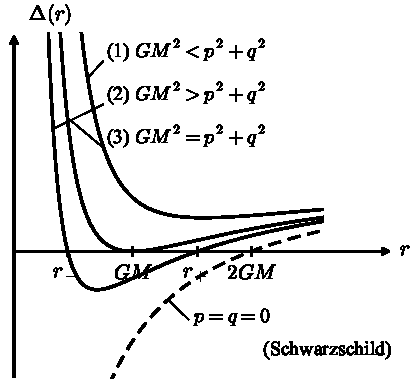
\includegraphics[width=0.72\textwidth]{fig_6.2.pdf}
\caption*{图 6.2\quad Reissner–Nordström 解的函数 $\Delta(r)=1-2GM/r+G(Q^{2}+P^{2})/r^{2}$；零点标示事件视界所在的位置。}
\end{figure}
如图 6.2 所示，随着 $GM^{2}$ 与 $Q^{2}+P^{2}$ 相对大小的不同，这可能给出两个、一个或零个解。于是我们逐个考察各种情形。

\subsection*{情形一：$GM^{2}<Q^{2}+P^{2}$}

这种情形下，系数 $\Delta$ 总为正（永不为零），度规在 $(t,r,\theta,\phi)$ 坐标中一直直到 $r=0$ 都完全正则。坐标 $t$ 总是类时的，而 $r$ 总是类空的。但 $r=0$ 处依然有奇点，只是现在它是一条类时线。由于不存在事件视界，观者前往奇点、看过一眼再返回报告所见，没有任何阻碍。这就是前面讨论过的裸奇点。对测地线的仔细分析表明，奇点是排斥的——类时测地线永远不会与 $r=0$ 相交；它们只是靠近，然后掉头离去。（类光测地线可以到达奇点，非测地线的类时曲线也可以。）

% ---- 书页 257 / p272 ----
\begin{figure}[H]
\centering
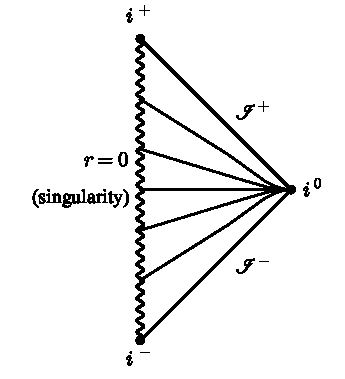
\includegraphics[width=0.72\textwidth]{fig_6.3.pdf}
\caption*{图 6.3\quad Reissner–Nordström 解在 $Q^{2}+P^{2}>GM^{2}$ 时的共形图。原点处有一个裸奇点。}
\end{figure}

当 $r\to\infty$ 时解趋近于平直时空，而且正如我们刚刚看到的，因果结构看上去处处正常。因此共形图就会与 Minkowski 空间的一模一样，只不过现在 $r=0$ 是一个奇点，如图 6.3 所示。

奇点的裸露冒犯了我们的体面感，也同样冒犯了宇宙监督假设。实际上，我们决不应指望引力坍缩的结果会是一个 $GM^{2}<Q^{2}+P^{2}$ 的黑洞。粗略地说，这个条件说的是，黑洞的总能量比单独电磁场贡献的能量还要少——也就是说，携带电荷的那些物质，其质量必须为负。因此这个解通常被认为是非物理的。还要注意，这个时空中不存在任何 Cauchy 面，因为类时线可以在奇点处开始或终止。

\subsection*{情形二：$GM^{2}>Q^{2}+P^{2}$}

我们预期这种情形适用于现实的引力坍缩；电磁场中的能量小于总能量。此时度规系数 $\Delta(r)$ 在 $r$ 很大和很小时都为正，而在两个零点 $r_{\pm}=GM\pm\sqrt{G^{2}M^{2}-G(Q^{2}+P^{2})}$ 之间为负。度规在 $r_{+}$ 和 $r_{-}$ 两处都有坐标奇点；与 Schwarzschild 的情形一样，这两处都可以通过坐标变换消去。

由 $r=r_{\pm}$ 定义的曲面都是类光的，而且二者都是事件视界。$r=0$ 处的奇点是一条类时线，而不像 Schwarzschild 中那样是一个类空曲面。如果你是一个从远处落入黑洞的观者，$r_{+}$ 就好比 Schwarzschild 度规中的 $2GM$：在这个半径处，$r$ 从类空坐标切换成类时坐标，你必然朝 $r$ 减小的方向运动。黑洞外面的目击者也会看到同样的
% ---- 书页 258 / p273 ----
现象，与不带电黑洞外面的情形相同——落入的观者看上去运动得越来越慢，红移也越来越厉害。

但是，从 $r_{+}$ 一路坠向越来越小的半径这种不可避免的坠落，只会持续到你抵达类光曲面 $r=r_{-}$ 为止；在那里 $r$ 重新变回类空坐标，朝 $r$ 减小方向的运动便可以止住。因此你并不一定要撞上 $r=0$ 处的奇点；这是意料之中的，因为 $r=0$ 是一条类时线（因而未必处在你的未来之中）。实际上，你既可以选取继续走向 $r=0$，也可以开始朝 $r$ 增大的方向折返，重新穿过 $r=r_{-}$ 处的类光曲面。此后 $r$ 将再一次成为类时坐标，只不过取向反了过来；你被迫朝 $r$ \emph{增大}的方向运动。最终你会再一次被抛过 $r=r_{+}$，就仿佛从一个白洞里冒出来、进入宇宙的其余部分。从这里你又可以选取回到黑洞中去——这一次是另一个洞，与你最初进入的那个不同——并且随你喜欢把这样的旅行重复多少次。这个小故事对应于图 6.4 中的共形图；当然，通过选取适当的坐标并把 Reissner–Nordström 度规解析延拓到极致，可以更严格地把它推导出来。

\begin{figure}[H]
\centering
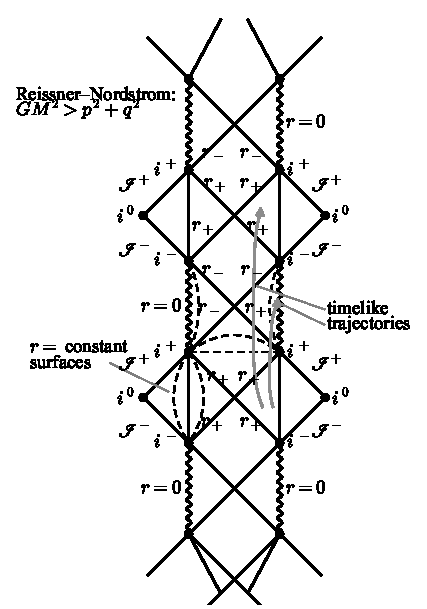
\includegraphics[width=0.72\textwidth]{fig_6.4.pdf}
\caption*{图 6.4\quad Reissner–Nordström 解在 $GM^{2}>Q^{2}+P^{2}$ 时的共形图。黑洞外部区域有无穷多个副本。}
\end{figure}

% ---- 书页 259 / p274 ----
\begin{figure}[H]
\centering
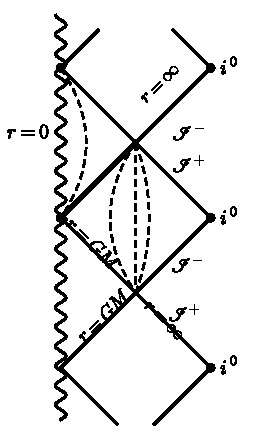
\includegraphics[width=0.72\textwidth]{fig_6.5.pdf}
\caption*{图 6.5\quad 极端 Reissner–Nordström 解（$GM^{2}=Q^{2}+P^{2}$）的共形图。原点处有一个裸奇点，外部区域则有无穷多个。}
\end{figure}

这番情景里有多少是科学、有多少是科学幻想呢？大概科学不多。如果你从一位身处黑洞内部、正要穿过 $r=r_{-}$ 处事件视界的观者的角度来考虑这个世界，你会注意到，这位观者可以回溯时间，看到外部（渐近平直）宇宙的整部历史——至少从黑洞看来是如此。但是，观者是在自己有限的固有时间内看到这段（无限长的）历史的——于是，当观者接近 $r_{-}$ 时，到达他们的任何信号都会被无限蓝移。因此，任何进入 RN 黑洞的非球对称微扰，都很可能会剧烈地扰动我们所描述的几何。真实的几何会是什么样子很难说，但没有很好的理由相信它必定包含无穷多个通过种种虫洞彼此连通的渐近平直区域。\footnote{关于这个问题的一些研究，见 E. Poisson and W. Israel, \emph{Phys.\ Rev.\ D} \textbf{41}, 1796 (1990).}

\subsection*{情形三：$GM^{2}=Q^{2}+P^{2}$}

这种情形称为\textbf{极端}（extremal）Reissner–Nordström 解。一方面，极端黑洞是一件有趣的理论玩具；在研究黑洞在量子引力中扮演的角色时，人们经常考察这个解。在超对称理论中，极端黑洞可以让某些对称性保持不破缺，这给计算带来极大的方便。另一方面，它看上去是不稳定的，因为只要加入一点点物质，它就会变成情形二。

极端黑洞的 $\Delta(r)$ 只在单个半径 $r=GM$ 处为零。这代表一个事件视界，但 $r$ 坐标永远不是类时的；它在 $r=GM$ 处变成类光的，而在两侧都是类空的。与其他情形一样，$r=0$ 处的奇点是一条类时线。所以对这个黑洞来说，你同样可以避开奇点，继续向未来运动到渐近平直区域的额外副本中去，只不过奇点总是“在左边”。共形图如图 6.5 所示。

极端黑洞的一个迷人性质是，质量在某种意义上被电荷平衡了。更具体地说，两个携带同号电荷的极端黑洞会彼此产生引力吸引，却又彼此产生电磁排斥，而这两种效应恰好抵消。事实上，对于相耦合的 Einstein–Maxwell 方程组，我们能找到\emph{精确}解，表示处在稳定位形中的任意数目的此类黑洞。为看清这一点，先回到 Reissner–Nordström 度规本身；为简单起见，我们只考虑电荷而不考虑磁荷。在极端性条件下 $GM^{2}=Q^{2}$，度规化为
\begin{equation*}
\mathrm{d}s^{2} = -\left(1-\frac{GM}{r}\right)^{2}\mathrm{d}t^{2} + \left(1-\frac{GM}{r}\right)^{-2}\mathrm{d}r^{2} + r^{2}\mathrm{d}\Omega^{2}.
\tag{6.58}
\end{equation*}
通过定义一个平移的径向坐标
\begin{equation*}
\rho = r - GM,
\tag{6.59}
\end{equation*}

% ---- 书页 260 / p275 ----
度规便取各向同性的形式
\begin{equation*}
\mathrm{d}s^{2} = -H^{-2}(\rho)\mathrm{d}t^{2} + H^{2}(\rho)\left[\mathrm{d}\rho^{2} + \rho^{2}\mathrm{d}\Omega^{2}\right],
\tag{6.60}
\end{equation*}
其中
\begin{equation*}
H(\rho) = 1 + \frac{GM}{\rho}.
\tag{6.61}
\end{equation*}
因为 $\mathrm{d}\rho^{2}+\rho^{2}\mathrm{d}\Omega^{2}$ 正是三个空间维度中的平直度规，我们同样可以把式 (6.60) 写成
\begin{equation*}
\mathrm{d}s^{2} = -H^{-2}(\vec{x})\mathrm{d}t^{2} + H^{2}(\vec{x})\left[\mathrm{d}x^{2} + \mathrm{d}y^{2} + \mathrm{d}z^{2}\right],
\tag{6.62}
\end{equation*}
其中 $H$ 可以写成
\begin{equation*}
H = 1 + \frac{GM}{|\vec{x}|}.
\tag{6.63}
\end{equation*}
在原先的 $r$ 坐标中，极端解的电场可以用矢势 $A_{\mu}$ 表示为
\begin{equation*}
E_{r} = F_{rt} = \frac{Q}{r^{2}} = \partial_{r}A_{0},
\tag{6.64}
\end{equation*}
其中矢势的类时分量为
\begin{equation*}
A_{0} = -\frac{Q}{r},
\tag{6.65}
\end{equation*}
并且我们设想空间分量为零（已经把磁场设为零）。在新的 $\rho$ 坐标下，再加上极端性条件 $Q^{2}=GM^{2}$，上式变为
\begin{equation*}
A_{0} = -\frac{\sqrt{G}M}{\rho+GM},
\tag{6.66}
\end{equation*}
或者等价地写成
\begin{equation*}
\sqrt{G}\,A_{0} = H^{-1}-1.
\tag{6.67}
\end{equation*}
但现在让我们忘掉 $H$ 满足式 (6.61) 这件事，径直把度规 (6.62) 和静电势 (6.67) 代入 Einstein 方程与麦克斯韦方程组，设想 $H$ 不依赖于时间（$\partial_{0}H=0$）但除此之外不受任何约束。我们可以直截了当地证明（见习题）：任何一个不依赖于时间、且满足
\begin{equation*}
\nabla^{2}H = 0,
\tag{6.68}
\end{equation*}
（其中 $\nabla^{2}=\partial_{x}^{2}+\partial_{y}^{2}+\partial_{z}^{2}$）的函数 $H(\vec{x})$，都能让这两组方程同时得到满足。这其实就是拉普拉斯方程，而且很容易写出所有在无穷远处表现良好的解；它们的形式为

% ---- 书页 261 / p276 ----
\begin{equation*}
H = 1 + \sum_{a=1}^{N}\frac{GM_{a}}{|\vec{x}-\vec{x}_{a}|},
\tag{6.69}
\end{equation*}
其中 $\vec{x}_{a}$ 给出某组 $N$ 个空间点。这些点描述了 $N$ 个极端 RN 黑洞所在的位置，各黑洞的质量为 $M_{a}$，电荷为 $Q_{a}=\sqrt{G}M_{a}$。这个多极端黑洞度规无疑是 Einstein 方程最引人注目的精确解之一。

\section{转动（Kerr）黑洞}

关于带电解，我们本来还可以多谈不少细节，但我们还是接着讲转动黑洞吧。在这种情形下寻找度规的精确解要困难得多，因为我们已经放弃了球对称性。我们转而寻找绕转动轴具有轴对称性、同时又是稳态的（即存在一个类时 Killing 矢量的）解。虽然 Schwarzschild 解和 Reissner–Nordström 解在广义相对论问世后不久就被发现了，但转动黑洞的解直到 1963 年才由 Kerr 找到。他的结果——\textbf{Kerr 度规}（Kerr metric）——就是下面这团乱麻：
\begin{equation*}
\boxed{\begin{aligned}
\mathrm{d}s^{2} &= -\left(1-\frac{2GMr}{\rho^{2}}\right)\mathrm{d}t^{2} - \frac{2GMar\sin^{2}\theta}{\rho^{2}}\left(\mathrm{d}t\,\mathrm{d}\phi + \mathrm{d}\phi\,\mathrm{d}t\right)\\
&\quad + \frac{\rho^{2}}{\Delta}\mathrm{d}r^{2} + \rho^{2}\mathrm{d}\theta^{2} + \frac{\sin^{2}\theta}{\rho^{2}}\left[(r^{2}+a^{2})^{2} - a^{2}\Delta\sin^{2}\theta\right]\mathrm{d}\phi^{2},
\end{aligned}}
\tag{6.70}
\end{equation*}
其中
\begin{equation*}
\boxed{\,\Delta(r) = r^{2} - 2GMr + a^{2}\,}
\tag{6.71}
\end{equation*}
以及
\begin{equation*}
\boxed{\,\rho^{2}(r,\theta) = r^{2} + a^{2}\cos^{2}\theta.\,}
\tag{6.72}
\end{equation*}
两个常数 $M$ 和 $a$ 参数化了各种可能的解。要验证质量 $M$ 确实等于 Komar 能量 (6.38) 并不难，只是繁琐；而 $a$ 是单位质量的角动量，
\begin{equation*}
a = J/M,
\tag{6.73}
\end{equation*}
其中 $J$ 是 Komar 角动量 (6.48)。要把电荷和磁荷 $Q$ 与 $P$ 也包括进来很容易，只需把 $2GMr$ 换成 $2GMr-G(Q^{2}+$

% ---- 书页 262 / p277 ----
$P^{2})$；得到的结果就是\textbf{Kerr–Newman 度规}（Kerr–Newman metric）。与之相联系的 1-形式势具有如下非零分量
\begin{equation*}
A_{t} = \frac{Qr - Pa\cos\theta}{\rho^{2}}, \qquad A_{\phi} = \frac{-Qar\sin^{2}\theta + P(r^{2}+a^{2})\cos\theta}{\rho^{2}}.
\tag{6.74}
\end{equation*}
所有本质性的现象在电荷不存在时依然保持，所以从现在起我们令 $Q=P=0$。

坐标 $(t,r,\theta,\phi)$ 就是所谓的\textbf{Boyer–Lindquist 坐标}（Boyer–Lindquist coordinates）。很容易验证，当 $a\to 0$ 时它们退化为 Schwarzschild 坐标。然而，如果保持 $a$ 不动而让 $M\to 0$，我们得到的仍是平直时空，只不过不是用普通的极坐标来表示的。此时度规变为
\begin{equation*}
\mathrm{d}s^{2} = -\mathrm{d}t^{2} + \frac{r^{2}+a^{2}\cos^{2}\theta}{r^{2}+a^{2}}\mathrm{d}r^{2} + \left(r^{2}+a^{2}\cos^{2}\theta\right)^{2}\mathrm{d}\theta^{2} + \left(r^{2}+a^{2}\right)\sin^{2}\theta\,\mathrm{d}\phi^{2},
\tag{6.75}
\end{equation*}
我们认出它的空间部分正是用椭球坐标表示的平直空间，如图 6.6 所示。这些坐标与欧几里得三维空间中的笛卡尔坐标之间的关系是
\begin{align*}
x &= \left(r^{2}+a^{2}\right)^{1/2}\sin\theta\cos\phi\\
y &= \left(r^{2}+a^{2}\right)^{1/2}\sin\theta\sin\phi\\
z &= r\cos\theta.
\tag{6.76}
\end{align*}

度规 (6.70) 有两个 Killing 矢量，二者都是显而易见的；由于度规系数不依赖于 $t$ 和 $\phi$，$K=\partial_{t}$ 与 $R=\partial_{\phi}$ 都是 Killing 矢量。当然，$R^{\mu}$ 表达的是解的轴对称性。矢量 $K^{\mu}$ 并不与 $t=$ 常数的超曲面正交，实际上也不与任何超曲面正交；因此这个度规是稳态的，但不是
% 本块末句在原书书页263顶部继续（“static. This makes sense; ...”），下一块请用 %JOIN% 续接本句。
静态的。这是有道理的：黑洞在转动，所以它不是静态的；但它在所有时刻都以完全相同的方式转动，所以它是稳态的。或者也可以这样理解：这个度规不可能是静态的，因为它不具有时间反演不变性——时间反演会把黑洞的角动量反过来。

\begin{figure}[H]
\centering
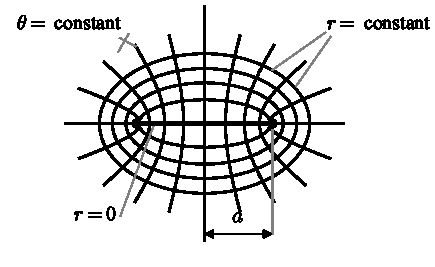
\includegraphics[width=0.72\textwidth]{fig_6.6.pdf}
\caption*{图 6.6\quad Kerr 度规中使用的椭球坐标 $(r,\theta)$。$r=0$ 是一个二维圆盘；$r=0$ 与 $\theta=\pi/2$ 的交集是这个圆盘边界上的圆环。}
\end{figure}

% ---- 书页 263 / p278 ----（本页第一段已在上面 tail 中接续，正文自第二段起）

Kerr 度规还拥有一个 Killing 张量（Killing tensor）。第 3 章中曾把它定义为任何满足如下条件的对称 $(0,n)$ 张量 $\sigma_{\mu_{1}\cdots\mu_{n}}$：
\begin{equation*}
\nabla_{(\lambda}\sigma_{\mu_{1}\cdots\mu_{n})} = 0.
\tag{6.77}
\end{equation*}
在 Kerr 几何中，我们可以定义 $(0,2)$ 张量
\begin{equation*}
\sigma_{\mu\nu} = 2\rho^{2}l_{(\mu}n_{\nu)} + r^{2}g_{\mu\nu}.
\tag{6.78}
\end{equation*}
在这个表达式中，两个矢量 $l$ 和 $n$（升指标后）为
\begin{gather*}
l^{\mu} = \frac{1}{\Delta}\left(r^{2}+a^{2},\, \Delta,\, 0,\, a\right)\\
n^{\mu} = \frac{1}{2\rho^{2}}\left(r^{2}+a^{2},\, -\Delta,\, 0,\, a\right).
\tag{6.79}
\end{gather*}
这两个矢量都是类光的，并且满足
\begin{equation*}
l^{\mu}l_{\mu} = 0,\qquad n^{\mu}n_{\mu} = 0,\qquad l^{\mu}n_{\mu} = -1.
\tag{6.80}
\end{equation*}
有了这些定义，你可以自己验证 $\sigma_{\mu\nu}$ 是一个 Killing 张量。

我们为 Kerr 选定的坐标，使得事件视界出现在那些让 $g^{rr}=0$ 的固定 $r$ 值处。由于 $g^{rr}=\Delta/\rho^{2}$，而 $\rho^{2}\geq 0$，这发生在
\begin{equation*}
\Delta(r) = r^{2} - 2GMr + a^{2} = 0.
\tag{6.81}
\end{equation*}
与 Reissner–Nordström 解一样，这里有三种可能性：$GM>a$、$GM=a$ 和 $GM<a$。最后一种情形的特征是存在裸奇点，而极端情形 $GM=a$ 是不稳定的，正如 Reissner–Nordström 情形一样。由于这些情形在物理上的重要性较低，我们将集中关注 $GM>a$。这时 $\Delta$ 在两个半径处为零，由
\begin{equation*}
r_{\pm} = GM \pm \sqrt{G^{2}M^{2}-a^{2}}.
\tag{6.82}
\end{equation*}
给出。这两个半径都是类光曲面，我们将会看到它们正是事件视界；Kerr 黑洞的侧视图见图 6.7。对这些曲面的分析与 Reissner–Nordström 情形极为类似；不难找到穿过视界延拓的坐标。

由于 Kerr 是稳态而非静态的，$r_{\pm}$ 处的事件视界并不是渐近时间平移 Killing 矢量 $K=\partial_t$ 的 Killing 视界。$K^{\mu}$ 的模由
\begin{equation*}
K^{\mu}K_{\mu} = -\frac{1}{\rho^{2}}\left(\Delta - a^{2}\sin^{2}\theta\right).
\tag{6.83}
\end{equation*}
给出。

% ---- 书页 264 / p279 ----

\begin{figure}[H]
\centering
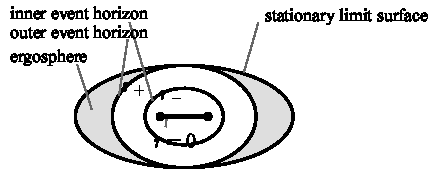
\includegraphics[width=0.72\textwidth]{fig_6.7.pdf}
\caption*{图 6.7\quad Kerr 解周围的视界结构（侧视图）。事件视界是类光曲面，它标示出一条分界：越过它之后就不可能再返回空间的某个区域。与此不同，静止极限面除了与事件视界相切之处（两极）以外都是类时的；它代表越过之后便无法保持静止观者身份的地方。静止极限面与外侧事件视界之间的能层（ergosphere）是一个可以进入、也可以再离开、但不能在其中保持静止的区域。}
\end{figure}

在外侧事件视界处它并不为零；事实上，在 $r=r_{+}$（此处 $\Delta=0$）我们有
\begin{equation*}
K^{\mu}K_{\mu} = \frac{a^{2}}{\rho^{2}}\sin^{2}\theta \geq 0.
\tag{6.84}
\end{equation*}
因此，这个 Killing 矢量在外侧视界处已经是类空的了，只有在北极和南极（$\theta=0,\pi$）处它是类光的。$K^{\mu}K_{\mu}=0$ 的点的轨迹当然就是静止极限面，由
\begin{equation*}
(r-GM)^{2} = G^{2}M^{2} - a^{2}\cos^{2}\theta,
\tag{6.85}
\end{equation*}
给出，而外侧事件视界则由
\begin{equation*}
(r_{+}-GM)^{2} = G^{2}M^{2} - a^{2}.
\tag{6.86}
\end{equation*}
给出。于是，这两个曲面之间存在一个区域，称为\textbf{能层}（ergosphere）。在能层内部，你必须沿着黑洞转动的方向运动（即 $\phi$ 方向）；不过，你仍然可以朝事件视界运动，也可以远离它（要退出能层也没有任何麻烦）。显然，甚至在穿越视界之前，能层就是一个可能发生有趣事情的地方；详情后述。

在急着画共形图之前，我们需要弄清楚真正的曲率奇点的性质；在这个时空中，它并不位于 $r=0$ 处，而是位于 $\rho=0$ 处（曲率不变量 $R_{\rho\sigma\mu\nu}R^{\rho\sigma\mu\nu}$ 在那里发散）。由于 $\rho^{2}=r^{2}+a^{2}\cos^{2}\theta$ 是两个明显非负的量之和，只有当两者同时为零时它才可能为零，即
\begin{equation*}
r = 0,\qquad \theta = \frac{\pi}{2}.
\tag{6.87}
\end{equation*}

% ---- 书页 265 / p280 ----

这个结果看上去有点滑稽，但请记住 $r=0$ 不是空间中的一个点，而是一个圆盘；满足 $r=0$、$\theta=\pi/2$ 的点集实际上就是这个圆盘边缘上的\emph{环}。转动把 Schwarzschild 奇点“软化”了，将它摊开成一个环。

如果你走进环内会发生什么？仔细的解析延拓（我们不打算真的去做）将会揭示，你会到达另一个渐近平直的时空，但它并不是你来自的那个时空的全同副本。新时空由 $r<0$ 的 Kerr 度规描述。结果是 $\Delta$ 永不为零，从而不存在视界。共形图（图 6.8）与 Reissner–Nordström 的情形非常相像，只是现在你可以穿过奇点。由于 Kerr 度规不是球对称的，共形图也就不像前面几种情形那样忠实；图上的一个点代表固定的 $t$ 和 $r$ 值，而对于不同的 $\theta$ 值，它将有不同的几何。

\begin{figure}[H]
\centering
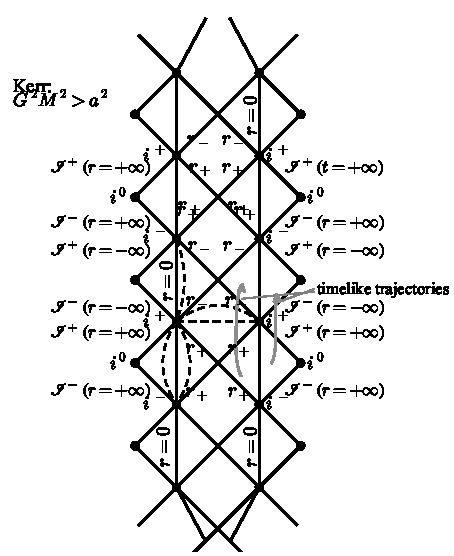
\includegraphics[width=0.72\textwidth]{fig_6.8.pdf}
\caption*{图 6.8\quad $G^{2}M^{2}>a^{2}$ 的 Kerr 解的共形图。与类似的带电解一样，黑洞外部的区域存在着无穷多个副本。}
\end{figure}

% ---- 书页 266 / p281 ----

我们不仅有这些经由黑洞与我们所在区域相连的、彼此不同的渐近平直区域所带来的通常怪异性，而且环奇点附近的区域还有额外的病态之处：闭合类时曲线（closed timelike curves，CTC）。如果你考虑一些在 $\phi$ 方向绕行、同时保持 $\theta$ 和 $t$ 固定、$r$ 取很小负值的轨迹，沿这样一条路径的线元是
\begin{equation*}
ds^{2} \approx a^{2}\left(1+\frac{2GM}{r}\right)\mathrm{d}\phi^{2},
\tag{6.88}
\end{equation*}
对于很小的负 $r$，它是负的。由于这些路径是闭合的，它们显然就是 CTC。因此，你有可能在过去遇见你自己，以及随之而来的一切。

当然，我们关于 Kerr 解析延拓所说的一切，都带有我们在讨论 Schwarzschild 和 Reissner–Nordström 时提到过的同样的告诫；真实的引力坍缩不太可能形成这些古怪的时空。尽管如此，拥有精确解总是有用的。此外，对于 Kerr 度规，即使我们停留在事件视界之外，奇怪的事情也在发生，现在我们就转向这些事情。

我们首先更仔细地考察黑洞的角速度。显然，常规的角速度定义必须稍加修改，才能应用于像时空度规这样抽象的对象。让我们考虑在 Kerr 黑洞的赤道面（$\theta=\pi/2$）内、半径 $r$ 处沿 $\phi$ 方向发射的一个光子的命运。它发射的那一瞬间，其动量在 $r$ 和 $\theta$ 方向都没有分量，因此轨迹为类光的条件是
\begin{equation*}
ds^{2} = 0 = g_{tt}\mathrm{d}t^{2} + g_{t\phi}\left(\mathrm{d}t\,\mathrm{d}\phi + \mathrm{d}\phi\,\mathrm{d}t\right) + g_{\phi\phi}\mathrm{d}\phi^{2}.
\tag{6.89}
\end{equation*}
这可以立即解出
\begin{equation*}
\frac{\mathrm{d}\phi}{\mathrm{d}t} = -\frac{g_{t\phi}}{g_{\phi\phi}} \pm \sqrt{\left(\frac{g_{t\phi}}{g_{\phi\phi}}\right)^{2} - \frac{g_{tt}}{g_{\phi\phi}}}.
\tag{6.90}
\end{equation*}
如果在 Kerr 度规的静止极限面上计算这个量，就有 $g_{tt}=0$，两个解为
\begin{equation*}
\frac{\mathrm{d}\phi}{\mathrm{d}t} = 0,\qquad \frac{\mathrm{d}\phi}{\mathrm{d}t} = \frac{a}{2G^{2}M^{2}+a^{2}}.
\tag{6.91}
\end{equation*}
非零解与 $a$ 同号；我们把它解释为光子绕黑洞运动的方向与黑洞转动的方向相同。零解则意味着，沿逆着黑洞转动方向射出的光子在这个坐标系中完全不动。注意，我们并没有给出光子轨迹的完整解，只是证明了它的瞬时速度为零。这就是著名的“参考系拖曳”（dragging of inertial frames）现象的一个例子；
% ---- 书页 267 / p282 ----
它将在第 7 章的一道习题中得到更多探讨。有质量的粒子必定比光子运动得慢，一旦进入静止极限面之内，它们就不可避免地被拖着随黑洞一起转动。当我们向位于 $r_{+}$ 处的外侧事件视界靠近时，这种拖曳仍在继续；我们可以定义事件视界本身的角速度 $\Omega_{\mathrm{H}}$，即粒子在视界处的最小角速度。直接由式 (6.90) 得到
\begin{equation*}
\Omega_{\mathrm{H}} = \left(\frac{\mathrm{d}\phi}{\mathrm{d}t}\right)_{-}(r_{+}) = \frac{a}{r_{+}^{2}+a^{2}}.
\tag{6.92}
\end{equation*}

\section{Penrose 过程与黑洞热力学}

黑洞热力学是广义相对论中最引人入胜、也最神秘的课题之一。不过，为了走到那里，让我们先从一件看上去非常直截了当的事情开始：Kerr 度规中沿测地线的运动。我们知道，如果考虑与 Killing 矢量 $K=\partial_t$ 和 $R=\partial_\phi$ 相联系的守恒量，这样的讨论将会得到简化。就眼前的目的而言，我们可以把注意力限制在有质量的粒子上，对它们可以使用四维动量
\begin{equation*}
p^{\mu} = m\frac{\mathrm{d}x^{\mu}}{\mathrm{d}\tau},
\tag{6.93}
\end{equation*}
其中 $m$ 是粒子的静质量。于是，我们可以取粒子真实的能量和角动量作为我们的两个守恒量，
\begin{equation*}
E = -K_{\mu}p^{\mu} = m\left(1-\frac{2GMr}{\rho^{2}}\right)\frac{\mathrm{d}t}{\mathrm{d}\tau} + \frac{2mGMar}{\rho^{2}}\sin^{2}\theta\,\frac{\mathrm{d}\phi}{\mathrm{d}\tau}
\tag{6.94}
\end{equation*}
以及
\begin{equation*}
L = R_{\mu}p^{\mu} = -\frac{2mGMar}{\rho^{2}}\sin^{2}\theta\,\frac{\mathrm{d}t}{\mathrm{d}\tau} + \frac{m(r^{2}+a^{2})^{2}-m\Delta a^{2}\sin^{2}\theta}{\rho^{2}}\sin^{2}\theta\,\frac{\mathrm{d}\phi}{\mathrm{d}\tau}.
\tag{6.95}
\end{equation*}
这些定义与上一章中使用的守恒量定义有所不同，在上一章里 $E$ 和 $L$ 取的是\emph{每单位质量}的能量和角动量。当然，无论哪种取法，它们都是守恒的。

$E$ 的定义中有一个负号，这是因为在无穷远处 $K^{\mu}$ 和 $p^{\mu}$ 都是类时的，它们的内积为负，而我们希望能量是正的。然而在能层内部，$K^{\mu}$ 变成了类空的；因此我们可以设想有这样的粒子，使得
\begin{equation*}
E = -K_{\mu}p^{\mu} < 0.
\tag{6.96}
\end{equation*}

% ---- 书页 268 / p283 ----

这件事令我们感到的不安，多少可以因如下认识而缓解：只要在静止极限面之外，\emph{所有}粒子的能量都必定为正；因此，能层内部具有负能量的粒子，要么留在能层之中，要么若想逃出去，就必须被加速到能量变为正。

尽管如此，这一认识仍然开辟了一条从转动黑洞中汲取能量的途径；这个方法就是\textbf{Penrose 过程}（Penrose process）。想法很简单：从能层之外出发，你给自己装备一块大石头，跃向黑洞。如果我们把（你 $+$ 石头）这个系统的四维动量记为 $p^{(0)\mu}$，那么能量 $E^{(0)}=-K_{\mu}p^{(0)\mu}$ 无疑是正的，而且当你沿自己的测地线运动时它是守恒的。一旦你进入能层，就用尽全力、以非常特别的方式把石头猛掷出去。如果把你的动量记为 $p^{(1)\mu}$、石头的动量记为 $p^{(2)\mu}$，那么在你掷出石头的那一瞬间，正如狭义相对论中一样，我们有动量守恒：
\begin{equation*}
p^{(0)\mu} = p^{(1)\mu} + p^{(2)\mu}.
\tag{6.97}
\end{equation*}
与 Killing 矢量 $K_{\mu}$ 缩并，给出
\begin{equation*}
E^{(0)} = E^{(1)} + E^{(2)}.
\tag{6.98}
\end{equation*}
但是，如果我们设想你足够强壮（而且投掷得足够精准），你就可以按照式 (6.96) 来安排你的投掷，使得 $E^{(2)}<0$。此外，Penrose 还能够证明，你可以像图 6.9 那样安排初始轨迹和投掷，使得随后你沿一条测地线轨迹回到静止极限面之外、进入外部宇宙。由于你的能量沿途守恒，

\begin{figure}[H]
\centering
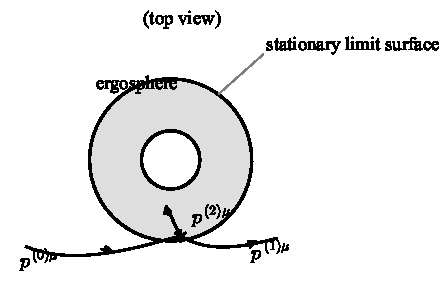
\includegraphics[width=0.72\textwidth]{fig_6.9.pdf}
\caption*{图 6.9\quad Penrose 过程（俯视图）。一个物体落向 Kerr 黑洞，并在能层之内（静止极限面以内、外侧事件视界之外）分裂为二。一块以负能量 $E^{(2)}$ 落入视界，另一块则以比原来落入物体更大的能量逃逸到无穷远。}
\end{figure}

% ---- 书页 269 / p284 ----

最终我们将有
\begin{equation*}
E^{(1)} > E^{(0)}.
\tag{6.99}
\end{equation*}
这样，你脱身而出时携带的能量就比你进入时\emph{更多}。

世上没有免费的午餐；你获得的能量来自某处，而那个某处就是黑洞。事实上，Penrose 过程是通过减小转动黑洞的角动量来从中汲取能量的；要让这个戏法奏效，你必须逆着黑洞的转动方向掷出石头。为了更精确地看清这一点，回忆一下我们在本章前文中的论断：稳态时空中的任何事件视界，对于某个 Killing 矢量来说都是一个 Killing 视界。对 Kerr 而言，这个矢量是时间平移和转动 Killing 矢量的线性组合，
\begin{equation*}
\chi^{\mu} = K^{\mu} + \Omega_{\mathrm{H}}R^{\mu},
\tag{6.100}
\end{equation*}
其中 $\Omega_{\mathrm{H}}$ 恰恰就是式 (6.92) 中定义的视界角速度。利用 $K=\partial_t$ 和 $R=\partial_\phi$，不难验证 $\chi^{\mu}$ 在外侧事件视界处变为类光。具有动量 $p^{(2)\mu}$ 的粒子“在时间中向前”地穿越事件视界，这一陈述不过是
\begin{equation*}
p^{(2)\mu}\chi_{\mu} < 0.
\tag{6.101}
\end{equation*}
代入 $E$ 和 $L$ 的定义，我们看到这个条件等价于
\begin{equation*}
L^{(2)} < \frac{E^{(2)}}{\Omega_{\mathrm{H}}}.
\tag{6.102}
\end{equation*}
既然我们已经安排 $E^{(2)}$ 为负、$\Omega_{\mathrm{H}}$ 为正，这就意味着粒子必须带有负的角动量——它在逆着黑洞转动的方向运动。一旦你逃出能层、石头落入事件视界之内，黑洞的质量和角动量就是原来的数值再加上石头所带来的负的贡献：
\begin{gather*}
\delta M = E^{(2)}\\
\delta J = L^{(2)},
\tag{6.103}
\end{gather*}
其中 $J=Ma$ 是黑洞的角动量。于是式 (6.102) 就变成了对角动量能够减小多少的一个限制：
\begin{equation*}
\delta J < \frac{\delta M}{\Omega_{\mathrm{H}}}.
\tag{6.104}
\end{equation*}
如果我们恰好达到这个极限——随着我们掷入的石头越来越接近类光——我们就得到了“理想”过程，其中 $\delta J = \delta M/\Omega_{\mathrm{H}}$。

现在我们将利用这些想法来验证：尽管你可以用 Penrose 过程从黑洞中汲取能量（从而减小 $M$），你却不能

% ---- 书页 270 / p285 ----

违反面积定理：事件视界的面积是不减的。虽然质量减小了，但角动量也必须减小，而且两者减小的组合方式只允许面积增加。为了看清这一点，我们来计算外侧事件视界的面积，它位于
\begin{equation*}
r_{+} = GM + \sqrt{G^{2}M^{2}-a^{2}}.
\tag{6.105}
\end{equation*}
视界上的诱导度规 $\gamma_{ij}$（其中 $i$ 和 $j$ 取遍 $\{\theta,\phi\}$）可以直截了当地求得：在式 (6.70) 中令 $r=r_{+}$（于是 $\Delta=0$）、$\mathrm{d}t=0$ 和 $\mathrm{d}r=0$：
\begin{align*}
\gamma_{ij}\,\mathrm{d}x^{i}\mathrm{d}x^{j} &= ds^{2}(\mathrm{d}t=0,\,\mathrm{d}r=0,\,r=r_{+})\\
&= (r_{+}^{2}+a^{2}\cos^{2}\theta)\mathrm{d}\theta^{2} + \left[\frac{(r_{+}^{2}+a^{2})^{2}\sin^{2}\theta}{r_{+}^{2}+a^{2}\cos^{2}\theta}\right]\mathrm{d}\phi^{2}.
\tag{6.106}
\end{align*}
于是，视界面积就是诱导体积元的积分，
\begin{equation*}
A = \int\sqrt{|\gamma|}\,\mathrm{d}\theta\,\mathrm{d}\phi.
\tag{6.107}
\end{equation*}
行列式为
\begin{equation*}
|\gamma| = (r_{+}^{2}+a^{2})^{2}\sin^{2}\theta,
\tag{6.108}
\end{equation*}
所以视界面积就是
\begin{equation*}
A = 4\pi(r_{+}^{2}+a^{2}).
\tag{6.109}
\end{equation*}

为了证明面积不会减小，更方便的做法是改用黑洞的\textbf{不可约质量}（irreducible mass），其定义为
\begin{align*}
M_{\mathrm{irr}}^{2} &= \frac{A}{16\pi G^{2}}\\
&= \frac{1}{4G^{2}}(r_{+}^{2}+a^{2})\\
&= \frac{1}{2}\left(M^{2}+\sqrt{M^{4}-(Ma/G)^{2}}\right)\\
&= \frac{1}{2}\left(M^{2}+\sqrt{M^{4}-(J/G)^{2}}\right).
\tag{6.110}
\end{align*}
经过一点计算，我们可以通过求导得到 $M_{\mathrm{irr}}$ 如何受质量或角动量变化的影响：
\begin{equation*}
\delta M_{\mathrm{irr}} = \frac{a}{4GM_{\mathrm{irr}}\sqrt{G^{2}M^{2}-a^{2}}}\left(\Omega_{\mathrm{H}}^{-1}\delta M - \delta J\right).
\tag{6.111}
\end{equation*}

% ---- 书页 271 / p286 ----

于是，我们的极限 (6.104) 就变成
\begin{equation*}
\delta M_{\mathrm{irr}} > 0.
\tag{6.112}
\end{equation*}
不可约质量永远无法减小；名称由此而来。由此可知，在把黑洞的转动减缓到零之前，我们能够从黑洞汲取的最大能量为
\begin{equation*}
M - M_{\mathrm{irr}} = M - \frac{1}{\sqrt{2}}\left(M^{2}+\sqrt{M^{4}-(J/G)^{2}}\right)^{1/2}.
\tag{6.113}
\end{equation*}
这种彻底汲取的结果，是一个质量为 $M_{\mathrm{irr}}$ 的 Schwarzschild 黑洞。事实证明，我们所能做到的最好情形是从一个极端 Kerr 黑洞出发；这样我们可以取出它总能量的大约 29\%。

$M_{\mathrm{irr}}$ 的不可约性直接引出这样一个事实：面积 $A$ 永不减小。由式 (6.110) 和 (6.111) 我们有
\begin{equation*}
\delta A = 8\pi G\,\frac{a}{\Omega_{\mathrm{H}}\sqrt{G^{2}M^{2}-a^{2}}}\left(\delta M - \Omega_{\mathrm{H}}\delta J\right),
\tag{6.114}
\end{equation*}
它可以改写为
\begin{equation*}
\delta M = \frac{\kappa}{8\pi G}\delta A + \Omega_{\mathrm{H}}\delta J,
\tag{6.115}
\end{equation*}
其中我们引入了
\begin{equation*}
\kappa = \frac{\sqrt{G^{2}M^{2}-a^{2}}}{2GM\left(GM+\sqrt{G^{2}M^{2}-a^{2}}\right)}.
\tag{6.116}
\end{equation*}
量 $\kappa$ 当然就是 Kerr 解的表面引力，你可以把式 (6.100) 代入式 (6.9) 来验证这一点。

像 (6.115) 这样的方程，最先促使人们开始思考黑洞与热力学之间的对应。考虑热力学第一定律，
\begin{equation*}
\mathrm{d}E = T\,\mathrm{d}S - p\,\mathrm{d}V,
\tag{6.117}
\end{equation*}
其中 $T$ 是温度，$S$ 是熵，$p$ 是压强，$V$ 是体积，因此 $p\,\mathrm{d}V$ 项代表我们对系统所做的功。很自然地，我们可以把式 (6.115) 中的 $\Omega_{\mathrm{H}}\delta J$ 项看成我们向黑洞投掷石头时对它所做的功。这样，如果我们把热力学量——能量、熵和温度——与黑洞的质量、面积和表面引力等同起来，这个对应就开始成形：
\begin{gather*}
E \leftrightarrow M\\
S \leftrightarrow A/4G\\
T \leftrightarrow \kappa/2\pi.
\tag{6.118}
\end{gather*}

% ---- 书页 272 / p287 ----

（记住，我们使用的单位制中 $\hbar=c=k=1$。）在经典广义相对论的语境中，这个类比本质上是完美的：热力学的每一条定律都对应着一条黑洞力学定律。处于热平衡的系统将弛豫到一个稳态，对应于稳态黑洞。热力学第零定律说，在热平衡中温度在整个系统中处处相同；对黑洞的类似陈述是：稳态黑洞在整个视界上具有恒定的表面引力。至少在使事件视界成为 Killing 视界的那同样的合理假设之下，这一点将会成立。正如我们已经看到的，第一定律 (6.117) 等价于 (6.115)。第二定律——熵永不减小——不过就是视界面积永不减小这一陈述。最后，第三定律的通常表述是：在任何物理过程中都不可能达到 $T=0$，或者说，当温度趋于零时熵必须趋于零。对黑洞来说，这不太灵验；事实证明 $\kappa=0$ 对应于极端黑洞，而极端黑洞的面积不一定为零。不过，热力学第三定律本身其实也不真正灵验，因为确实存在违反它的普通物理系统；第三定律适用于某些情形，但并不是真正基本的定律。

在提出对应关系 (6.118) 时，我们有点儿作弊了；你会注意到，把 $T\mathrm{d}S$ 与 $\kappa\mathrm{d}A/8\pi G$ 等同起来之后，我们并不知道如何分别归一化 $S/A$ 或 $T/\kappa$，只知道它们的组合。不过，正如我们将在第 9 章讨论的，Hawking 证明了黑洞背景中的量子场使得黑洞以温度 $T=\kappa/2\pi$ 发出辐射。一旦知道了这一点，我们就可以把 $A/4G$ 解释为黑洞的真实熵。Bekenstein 提出了\textbf{广义第二定律}（generalized second law）：物质与黑洞合起来的熵永不减小：
\begin{equation*}
\delta\left(S + \frac{A}{4G}\right) \geq 0.
\tag{6.119}
\end{equation*}
广义第二定律实际上可以在多种不同的假设下得到证明。不过，我们通常喜欢把系统的熵与可到达的量子态数目的对数联系起来。因此，这个概念与无毛定理之间存在着某种张力：无毛定理告诉我们，具有固定电荷、质量和自旋的黑洞，其可能的状态极少（事实上只有一个）。这种行为似乎在向我们暗示，它是量子力学与引力之间相互作用之深刻性质的一个表征。

\section{习题}

\textbf{1.}\quad 证明：耦合的 Einstein–Maxwell 方程组可以同时由度规 (6.62) 和静电势 (6.67) 求解，只要 $H(\vec{x})$ 满足拉普拉斯方程
\begin{equation*}
\nabla^{2}H = 0.
\tag{6.120}
\end{equation*}

\textbf{2.}\quad 考虑 Kerr 黑洞赤道面内无质量粒子的轨道，仿射参量为 $\lambda$。

\textbf{(a)}\quad 证明
\begin{equation*}
\left(\frac{\mathrm{d}r}{\mathrm{d}\lambda}\right)^{2} = \frac{\Sigma^{2}}{\rho^{4}}\left(E - LW_{+}(r)\right)\left(E - LW_{-}(r)\right),
\tag{6.121}
\end{equation*}
其中 $\Sigma^{2} = (r^{2}+a^{2})^{2} - a^{2}\Delta(r)\sin^{2}\theta$，$E$ 和 $L$ 是守恒的能量和角动量，而 $W_{\pm}(r)$ 的表达式则要你自己求出。

\textbf{(b)}\quad 利用这个结果，并假设 $\Sigma^{2}$ 处处大于零，证明：赤道面内光子的轨道不可能在外侧事件视界 $r_{+}$ 之内存在转折点。这意味着，入射光线一旦穿越 $r_{+}$ 就无法逃逸，所以它确实是一个事件视界。

% ---- 书页 273 / p288 ----

\textbf{3.}\quad 在存在电磁场的情况下，电荷为 $e$、质量为 $m$ 的粒子服从
\begin{equation*}
\frac{\mathrm{d}^{2}x^{\mu}}{\mathrm{d}\tau^{2}} + \Gamma^{\mu}_{\rho\sigma}\frac{\mathrm{d}x^{\rho}}{\mathrm{d}\tau}\frac{\mathrm{d}x^{\sigma}}{\mathrm{d}\tau} = \frac{e}{m}F^{\mu}{}_{\nu}\frac{\mathrm{d}x^{\nu}}{\mathrm{d}\tau}.
\tag{6.122}
\end{equation*}
设想这样一个粒子在电荷为 $Q$、质量为 $M$ 的 Reissner–Nordström 黑洞的场中运动。

\textbf{(a)}\quad 证明能量
\begin{equation*}
E = m\left(1 - \frac{2GM}{r} + \frac{GQ^{2}}{r^{2}}\right)\frac{\mathrm{d}t}{\mathrm{d}\tau} + \frac{eQ}{r}
\tag{6.123}
\end{equation*}
是守恒的。

\textbf{(b)}\quad Penrose 型的过程对带电黑洞行得通吗？对于最大的物理过程，黑洞质量的改变量 $\delta M$ 是多少？

\textbf{4.}\quad 考虑静态坐标下的 de Sitter 空间：
\begin{equation*}
ds^{2} = -\left(1 - \frac{\Lambda}{3}r^{2}\right)\mathrm{d}t^{2} + \frac{\mathrm{d}r^{2}}{1 - \frac{\Lambda}{3}r^{2}} + r^{2}\mathrm{d}\Omega^{2}.
\end{equation*}
这个空间有一个 Killing 矢量 $\partial_t$，它在 $r=0$ 附近是类时的，而在某个 Killing 视界上是类光的。试定出 Killing 视界的径向位置 $r_{\mathrm{K}}$。该视界的表面引力 $\kappa$ 是多少？考虑通过替换 $t\rightarrow i\tau$ 得到的 de Sitter 空间的欧氏号差版本。证明：只要把 $\tau$ 取成周期的，就可以通过一个坐标变换使欧氏度规在视界处正则。

\textbf{5.}\quad 一位观者沿周长为 $2\pi R$ 的圆轨道，绕着电荷为 $Q$、质量为 $M$ 的 Reissner–Nordström 黑洞运行，他所看到的磁场是什么？

\textbf{6.}\quad 考虑一个 Kerr 黑洞，在其赤道面内有一个质量可忽略的吸积盘（accretion disk）。假设盘中的粒子沿测地线运动（也就是说，忽略任何压强支撑）。现在进一步假设盘中含有一些铁原子，它们正被某个辐射源激发。当铁原子退激发时，它们会发出辐射，在它们自己的静止系中测量，其频率为已知的 $\nu_{0}$。假设我们在远离黑洞的地方探测这种辐射（我们也处在赤道面内）。从盘的任一边缘以及从盘的中心发出的光子，其观测频率各是多少？考虑盘与黑洞同向转动和反向转动这两种情形。我们能否利用这些测量来确定黑洞的质量和角动量？

 % 本文件由 scripts/assemble.py 自动装配，勿手改（改 parts/ 后重跑）
% 第7章 微扰理论与引力辐射

% 第7章 Perturbation Theory and Gravitational Radiation
\chapter{微扰理论与引力辐射}

\section{线性化引力与规范变换}

% ---- 书页 274 / p289 ----
我们最初推导 Einstein 方程的时候，是通过考虑 Newton 极限来确认自己走在正确的道路上。当时我们对这句话的理解是：不仅引力场是弱的，而且它是静态的（不含时间导数），检验粒子也在缓慢地运动。本章要描述的弱场极限限制要少一些：只假定场仍然是弱的，但它可以随时间变化，并且对检验粒子的运动不加任何限制。这将使我们能够讨论一些在 Newton 理论中缺席或含混的现象，例如引力辐射（场随时间变化）以及光线偏折（涉及快速运动的粒子）。

引力场的微弱，再一次表现为我们有能力把度规分解成平直的 Minkowski 度规加上一个小微扰，
\begin{equation*}
g_{\mu\nu} = \eta_{\mu\nu} + h_{\mu\nu}, \qquad |h_{\mu\nu}| \ll 1.
\tag{7.1}
\end{equation*}
我们将把自己限制在 $\eta_{\mu\nu}$ 取规范形式的坐标系中，即 $\eta_{\mu\nu} = \mathrm{diag}(-1,+1,+1,+1)$。$h_{\mu\nu}$ 是小量这一假设，使我们能够忽略任何高于该量一阶的东西，由此立即得到
\begin{equation*}
g^{\mu\nu} = \eta^{\mu\nu} - h^{\mu\nu},
\tag{7.2}
\end{equation*}
其中 $h^{\mu\nu} = \eta^{\mu\rho}\eta^{\nu\sigma}h_{\rho\sigma}$。与之前一样，我们可以用 $\eta^{\mu\nu}$ 和 $\eta_{\mu\nu}$ 升降指标，因为相应的修正将是微扰的高阶小量。事实上，我们可以把广义相对论的线性化版本（其中 $h_{\mu\nu}$ 的高于一阶的效应都被略去）看作是在平直背景时空上传播的一个对称张量场 $h_{\mu\nu}$ 的理论。这个理论在狭义相对论的意义下是洛伦兹不变的；在洛伦兹变换 $x^{\mu'} = \Lambda^{\mu'}{}_{\mu}x^{\mu}$ 之下，平直度规 $\eta_{\mu\nu}$ 不变，而微扰按下式变换
\begin{equation*}
h_{\mu'\nu'} = \Lambda^{\mu'}{}_{\mu}\Lambda^{\nu'}{}_{\nu}h_{\mu\nu}.
\tag{7.3}
\end{equation*}

% ---- 书页 275 / p290 ----
注意，我们本来也可以考虑 Minkowski 空间之外的某个其他背景时空上的小微扰。在那种情形下，度规将被写成 $g_{\mu\nu} = g_{\mu\nu}^{(0)} + h_{\mu\nu}$，而我们导出的将是关于一个在度规为 $g_{\mu\nu}^{(0)}$ 的弯曲空间上传播的对称张量的理论。例如在宇宙学中，这样的处理方式就是必需的。

我们想找出微扰 $h_{\mu\nu}$ 所服从的运动方程，它来自把 Einstein 方程考察到一阶。我们从 Christoffel 符号入手，它由下式给出
\begin{align*}
\Gamma^{\rho}_{\mu\nu} &= \frac{1}{2}g^{\rho\lambda}(\partial_{\mu}g_{\nu\lambda} + \partial_{\nu}g_{\lambda\mu} - \partial_{\lambda}g_{\mu\nu}) \\
&= \frac{1}{2}\eta^{\rho\lambda}(\partial_{\mu}h_{\nu\lambda} + \partial_{\nu}h_{\lambda\mu} - \partial_{\lambda}h_{\mu\nu}).
\tag{7.4}
\end{align*}
由于联络系数是一阶量，它们对 Riemann 张量的贡献将只来自 $\Gamma$ 的导数，而不含 $\Gamma^{2}$ 项。为方便起见降低一个指标，我们得到
\begin{align*}
R_{\mu\nu\rho\sigma} &= \eta_{\mu\lambda}\partial_{\rho}\Gamma^{\lambda}_{\nu\sigma} - \eta_{\mu\lambda}\partial_{\sigma}\Gamma^{\lambda}_{\nu\rho} \\
&= \frac{1}{2}(\partial_{\rho}\partial_{\nu}h_{\mu\sigma} + \partial_{\sigma}\partial_{\mu}h_{\nu\rho} - \partial_{\sigma}\partial_{\nu}h_{\mu\rho} - \partial_{\rho}\partial_{\mu}h_{\nu\sigma}).
\tag{7.5}
\end{align*}
对 $\mu$ 和 $\rho$ 缩并便得到 Ricci 张量，
\begin{equation*}
R_{\mu\nu} = \frac{1}{2}(\partial_{\sigma}\partial_{\nu}h^{\sigma}{}_{\mu} + \partial_{\sigma}\partial_{\mu}h^{\sigma}{}_{\nu} - \partial_{\mu}\partial_{\nu}h - \Box h_{\mu\nu}),
\tag{7.6}
\end{equation*}
它显然关于 $\mu$ 和 $\nu$ 对称。在这个表达式中，我们把微扰的迹定义为 $h = \eta^{\mu\nu}h_{\mu\nu} = h^{\mu}{}_{\mu}$，而 d'Alembert 算符就是平直空间中的那一个：$\Box = -\partial_{t}^{2} + \partial_{x}^{2} + \partial_{y}^{2} + \partial_{z}^{2}$。再一次缩并以得到 Ricci 标量，就有
\begin{equation*}
R = \partial_{\mu}\partial_{\nu}h^{\mu\nu} - \Box h.
\tag{7.7}
\end{equation*}
把这些都放在一起，我们就得到了 Einstein 张量：
\begin{align*}
G_{\mu\nu} &= R_{\mu\nu} - \frac{1}{2}\eta_{\mu\nu}R \\
&= \frac{1}{2}(\partial_{\sigma}\partial_{\nu}h^{\sigma}{}_{\mu} + \partial_{\sigma}\partial_{\mu}h^{\sigma}{}_{\nu} - \partial_{\mu}\partial_{\nu}h - \Box h_{\mu\nu} - \eta_{\mu\nu}\partial_{\rho}\partial_{\lambda}h^{\rho\lambda} + \eta_{\mu\nu}\Box h).
\tag{7.8}
\end{align*}
与我们把线性化理论理解为描述平直背景上的对称张量的理论相一致，线性化 Einstein 张量 (7.8) 可以通过对下面这个拉格朗日量关于 $h_{\mu\nu}$ 作变分而导出：
\begin{align*}
\mathcal{L} = \frac{1}{2}\Big[(\partial_{\mu}h^{\mu\nu})(\partial_{\nu}h) &- (\partial_{\mu}h^{\rho\sigma})(\partial_{\rho}h^{\mu}{}_{\sigma}) + \frac{1}{2}\eta^{\mu\nu}(\partial_{\mu}h^{\rho\sigma})(\partial_{\nu}h_{\rho\sigma}) \\
&- \frac{1}{2}\eta^{\mu\nu}(\partial_{\mu}h)(\partial_{\nu}h)\Big].
\tag{7.9}
\end{align*}
这个拉格朗日量是否恰当，请你在习题中加以验证。

% ---- 书页 276 / p291 ----
线性化场方程当然就是 $G_{\mu\nu} = 8\pi GT_{\mu\nu}$，其中 $G_{\mu\nu}$ 由式 (7.8) 给出，而 $T_{\mu\nu}$ 是能量-动量张量，按 $h_{\mu\nu}$ 的零阶计算。我们不把更高阶的修正包括进能量-动量张量，因为要使弱场极限适用，能量和动量的总量本身就必须很小。换句话说，$T_{\mu\nu}$ 中最低的非零阶自动与微扰具有相同的数量级。注意，最低阶下的守恒定律就是简单的 $\partial_{\mu}T^{\mu\nu} = 0$。我们常常关心的是真空方程，它一如既往就只是 $R_{\mu\nu} = 0$，其中 $R_{\mu\nu}$ 由式 (7.6) 给出。

有了线性化场方程，我们差不多就准备好着手求解它了。然而，我们首先应该处理规范不变性这个棘手的问题。这个问题之所以出现，是因为要求 $g_{\mu\nu} = \eta_{\mu\nu} + h_{\mu\nu}$ 并没有完全确定时空上的坐标系；可能存在别的坐标系，度规在其中仍然可以写成 Minkowski 度规加上一个小微扰，只不过微扰有所不同。因此，把度规分解成平直背景加微扰的做法并不是唯一的。为了考察这个问题，我们将利用附录 A 和附录 B 中讨论的关于微分同胚的思想；尚未读过那两节的读者可以跳到式 (7.14) 及其后的两段，那里包含了最关键的思想。

让我们从一种“高观点”（highbrow）的角度来思考规范不变性。线性化理论可以看作是一个支配平直背景上张量场行为的理论——这个观念可以借助一个\textbf{背景时空}（background spacetime）$M_{b}$、一个\textbf{物理时空}（physical spacetime）$M_{p}$ 以及一个微分同胚 $\phi : M_{b} \to M_{p}$ 来形式化。作为流形，$M_{b}$ 和 $M_{p}$ 是同一个（因为它们微分同胚），但我们设想它们拥有一些不同的张量场：在 $M_{b}$ 上我们定义了平直的 Minkowski 度规 $\eta_{\mu\nu}$，而在 $M_{p}$ 上有某个遵守 Einstein 方程的度规 $g_{\alpha\beta}$。（我们设想 $M_{b}$ 配有坐标 $x^{\mu}$，$M_{p}$ 配有坐标 $y^{\alpha}$，尽管这些坐标并不会扮演什么显要角色。）微分同胚 $\phi$ 使我们能够在背景时空与物理时空之间来回搬移张量，如图 7.1 所示。既然我们想把线性化理论构造成一个发生在平直背景时空上的理论，我们感兴趣的便是物理度规的拉回 $(\phi^{*}g)_{\mu\nu}$。我们可以把微扰定义为拉回后的物理度规与平直度规之差：

\begin{figure}[H]
\centering
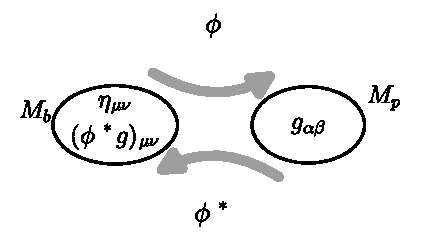
\includegraphics[width=0.72\textwidth]{fig_7.1.pdf}
\caption*{图 7.1\quad 一个微分同胚把背景时空 $M_{b}$（具有平直度规 $\eta_{\mu\nu}$）与物理时空 $M_{p}$ 联系起来。}
\end{figure}

% ---- 书页 277 / p292 ----
\begin{figure}[H]
\centering
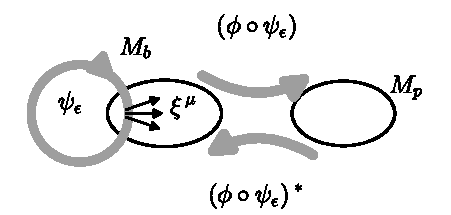
\includegraphics[width=0.72\textwidth]{fig_7.2.pdf}
\caption*{图 7.2\quad 由背景时空 $M_{b}$ 上的矢量场 $\xi^{\mu}$ 生成的单参数微分同胚族 $\psi_{\epsilon}$。}
\end{figure}
\begin{equation*}
h_{\mu\nu} = (\phi^{*}g)_{\mu\nu} - \eta_{\mu\nu}.
\tag{7.10}
\end{equation*}
根据这个定义，$h_{\mu\nu}$ 的分量没有理由必须是小的；不过，如果 $M_{p}$ 上的引力场是弱的，那么对某些微分同胚 $\phi$ 我们就会有 $|h_{\mu\nu}| \ll 1$。于是我们只把注意力限制在那些使这一点成立的微分同胚上。这样一来，$g_{\alpha\beta}$ 在物理时空上遵守 Einstein 方程这一事实，就意味着 $h_{\mu\nu}$ 在背景时空上将遵守线性化方程（因为 $\phi$ 作为微分同胚，同样可以用来拉回 Einstein 方程本身）。

在这种语言里，规范不变性问题不过是说，在 $M_{b}$ 与 $M_{p}$ 之间存在着大量“许可的”微分同胚（“许可”的意思是微扰是小的）。考虑背景时空上的一个矢量场 $\xi^{\mu}(x)$。这个矢量场生成一个单参数微分同胚族 $\psi_{\epsilon} : M_{b} \to M_{b}$，如图 7.2 所示。当 $\epsilon$ 足够小时，如果 $\phi$ 是一个使由式 (7.10) 定义的微扰很小的微分同胚，那么 $(\phi \circ \psi_{\epsilon})$ 也是，只不过微扰将取不同的值。具体地，我们可以定义一个以 $\epsilon$ 为参数的微扰族：
\begin{align*}
h^{(\epsilon)}_{\mu\nu} &= [(\phi \circ \psi_{\epsilon})^{*}g]_{\mu\nu} - \eta_{\mu\nu} \\
&= [\psi_{\epsilon}^{*}(\phi^{*}g)]_{\mu\nu} - \eta_{\mu\nu}.
\tag{7.11}
\end{align*}
第二个等号基于这样的事实：复合映射的拉回等于各拉回按相反次序的复合，而这又源于拉回本身就是沿与原映射相反的方向搬动事物。代入关系式 (7.10)，我们发现
\begin{align*}
h^{(\epsilon)}_{\mu\nu} &= \psi_{\epsilon}^{*}(h + \eta)_{\mu\nu} - \eta_{\mu\nu} \\
&= \psi_{\epsilon}^{*}(h_{\mu\nu}) + \psi_{\epsilon}^{*}(\eta_{\mu\nu}) - \eta_{\mu\nu},
\tag{7.12}
\end{align*}
这是因为两个张量之和的拉回等于各自拉回之和。现在我们动用 $\epsilon$ 是小量这一假设；此时 $\psi_{\epsilon}^{*}(h_{\mu\nu})$ 在最低阶下等于 $h_{\mu\nu}$，而另外两项则给我们一个李导数：

% ---- 书页 278 / p293 ----
\begin{align*}
h^{(\epsilon)}_{\mu\nu} &= \psi_{\epsilon}^{*}(h_{\mu\nu}) + \epsilon\left[\frac{\psi_{\epsilon}^{*}(\eta_{\mu\nu}) - \eta_{\mu\nu}}{\epsilon}\right] \\
&= h_{\mu\nu} + \epsilon\mathcal{L}_{\xi}\eta_{\mu\nu}.
\tag{7.13}
\end{align*}
在附录 B 中我们证明过，度规沿矢量场 $\xi_{\mu}$ 的李导数为 $\mathcal{L}_{\xi}g_{\mu\nu} = 2\nabla_{(\mu}\xi_{\nu)}$。在当前的情形下，背景度规是平直的，协变导数变成偏导数；因此我们有
\begin{equation*}
\boxed{\,h^{(\epsilon)}_{\mu\nu} = h_{\mu\nu} + 2\epsilon\partial_{(\mu}\xi_{\nu)}.\,}
\tag{7.14}
\end{equation*}
这个公式表示度规微扰在沿矢量场 $\epsilon\xi^{\mu}$ 的无穷小微分同胚下的改变；我们将把它称为线性化理论中的\textbf{规范变换}（gauge transformation）。

微分同胚 $\psi_{\epsilon}$ 给出了同一物理情形的不同表示，同时保持我们对微扰很小的要求。因此，结果 (7.12) 告诉我们，什么样的度规微扰描写的时空在物理上等价——即对某个矢量 $\xi^{\mu}$ 而言彼此相差 $2\epsilon\partial_{(\mu}\xi_{\nu)}$ 的那些时空。我们的理论在这种变换下的不变性，类似于电磁学中在 $A_{\mu} \to A_{\mu} + \partial_{\mu}\lambda$ 之下的传统规范不变性。（这个类比不同于我们在附录 J 中与电磁学画的另一个类比；那个类比把正交标架形式中的局部洛伦兹变换联系到内部矢量丛中基的改变。）在电磁学中，不变性之所以成立，是因为场强 $F_{\mu\nu} = \partial_{\mu}A_{\nu} - \partial_{\nu}A_{\mu}$ 在规范变换下保持不变；类似地，我们发现变换 (7.14) 使线性化 Riemann 张量改变
\begin{align*}
\delta R_{\mu\nu\rho\sigma} = \frac{1}{2}(&\partial_{\rho}\partial_{\nu}\partial_{\mu}\xi_{\sigma} + \partial_{\rho}\partial_{\nu}\partial_{\sigma}\xi_{\mu} + \partial_{\sigma}\partial_{\mu}\partial_{\nu}\xi_{\rho} + \partial_{\sigma}\partial_{\mu}\partial_{\rho}\xi_{\nu} \\
&- \partial_{\sigma}\partial_{\nu}\partial_{\mu}\xi_{\rho} - \partial_{\sigma}\partial_{\nu}\partial_{\rho}\xi_{\mu} - \partial_{\rho}\partial_{\mu}\partial_{\nu}\xi_{\sigma} - \partial_{\rho}\partial_{\mu}\partial_{\sigma}\xi_{\nu}) \\
&= 0.
\tag{7.15}
\end{align*}
我们对度规微扰的适当规范变换所作的抽象推导，由此得到印证：它使曲率（从而也使物理时空）保持不变。

规范不变性也可以从一条观点稍微“低”一些（lowbrow）、却直接得多的途径来理解，即无穷小坐标变换。我们的微分同胚 $\psi_{\epsilon}$ 可以看作是把坐标从 $x^{\mu}$ 变到 $x^{\mu} - \epsilon\xi^{\mu}$。（这个不合常规的负号来自如下事实：“新”度规是从沿积分曲线向前一小段距离处拉回的，而这等价于把坐标换成沿曲线向后一小段距离处的坐标。）按照坐标变换下张量变换的通常规则一步步推下去，你可以恰好导出 (7.14)——尽管你得稍微作点弊，把两个不同坐标系中张量的分量等同起来。

% ---- 书页 279 / p294 ----
\section{自由度}

有了线性化 Einstein 张量的表达式 (7.8) 和规范变换效应的表达式 (7.14)，我们本可以立刻着手选取规范并求解 Einstein 方程。不过，我们可以先在 Minkowski 背景时空中选定一个固定的惯性坐标系，把度规微扰的分量按照它们在空间转动下的变换性质加以分解，由此积累起一些额外的物理洞见。你也许会担心，这样的分解有悖于广义相对论的坐标无关精神，但它其实与把电磁场强张量分解成电场和磁场并没有什么不同。尽管 $\mathbf{E}$ 和 $\mathbf{B}$ 都是一个 (0, 2) 张量的分量，但有时不妨假想某位固定观者的角色，把它们当作三维矢量来看待。\footnote{这里的讨论沿循 E. Bertschinger, “Cosmological Dynamics,” a talk given at Summer School on Cosmology and Large Scale Structure (Session 60), Les Houches, France, 1--28 Aug 1993; http://arXiv.org/abs/astro-ph/9503125。Bertschinger 关注的是宇宙学微扰论，其中类空超曲面随时间膨胀，但把它特化到不膨胀宇宙的情形也很简单。}

度规微扰是一个 (0, 2) 张量，但它不是反对称的，而是对称的。在空间转动下，00 分量是标量，0i 分量（等于 i0 分量）构成一个三维矢量，ij 分量则构成一个两指标的对称空间张量。这个空间张量还可以进一步分解成迹与无迹两部分。（用群论的语言说，我们在寻找转动群的“不可约表示”。换句话说，我们把张量分解成一个个单独的部分，它们在空间转动下只变换成它们自身。）于是我们把 $h_{\mu\nu}$ 写成
\begin{align*}
h_{00} &= -2\Phi \\
h_{0i} &= w_{i} \\
h_{ij} &= 2s_{ij} - 2\Psi\delta_{ij},
\tag{7.16}
\end{align*}
其中 $\Psi$ 编码了 $h_{ij}$ 的迹，而 $s_{ij}$ 是无迹的：
\begin{align*}
\Psi &= -\frac{1}{6}\delta^{ij}h_{ij} \\
s_{ij} &= \frac{1}{2}\left(h_{ij} - \frac{1}{3}\delta^{kl}h_{kl}\delta_{ij}\right).
\tag{7.17}
\end{align*}
整个度规于是可以写成
\begin{equation*}
\boxed{\,\mathrm{d}s^{2} = -(1+2\Phi)\mathrm{d}t^{2} + w_{i}(\mathrm{d}t\,\mathrm{d}x^{i} + \mathrm{d}x^{i}\,\mathrm{d}t) + [(1-2\Psi)\delta_{ij} + 2s_{ij}]\mathrm{d}x^{i}\mathrm{d}x^{j}.\,}
\tag{7.18}
\end{equation*}

% ---- 书页 280 / p295 ----
我们还没有选取规范，也没有求解任何方程，只是定义了一些方便的记号。无迹张量 $s_{ij}$ 被称为应变（strain），我们将会看到，引力辐射就包含在它之中。有时把空间分量分解成迹与无迹两部分并无帮助，这时我们可以径直坚持用 $h_{ij}$；在具体情形中哪种记号合适就用哪种。注意，正如在第 1 章中那样，空间度规现在就是简单的 $\delta_{ij}$，我们可以随意升降空间指标而不改变分量。

为了体会度规微扰中各个不同场的物理诠释，我们来考虑由测地线方程描述的检验粒子的运动。式 (7.18) 相应的 Christoffel 符号是
\begin{align*}
\Gamma^{0}_{00} &= \partial_{0}\Phi \\
\Gamma^{i}_{00} &= \partial_{i}\Phi + \partial_{0}w_{i} \\
\Gamma^{0}_{j0} &= \partial_{j}\Phi \\
\Gamma^{i}_{j0} &= \partial_{[j}w_{i]} + \frac{1}{2}\partial_{0}h_{ij} \\
\Gamma^{0}_{jk} &= -\partial_{(j}w_{k)} + \frac{1}{2}\partial_{0}h_{jk} \\
\Gamma^{i}_{jk} &= \partial_{(j}h_{k)i} - \frac{1}{2}\partial_{i}h_{jk}.
\tag{7.19}
\end{align*}
在这些表达式里，我们坚持用 $h_{ij}$ 而不用 $s_{ij}$ 和 $\Psi$，因为它们只是以组合 $h_{ij} = 2s_{ij} - 2\Psi\delta_{ij}$ 的形式进入。一旦我们开始取迹以得到 Ricci 张量和 Einstein 方程，这种区分就会变得重要。既然我们已经固定了一个惯性系，方便的做法是把四维动量 $p^{\mu} = \mathrm{d}x^{\mu}/\mathrm{d}\lambda$（若粒子有质量，则 $\lambda = \tau/m$）用能量 $E$ 和三速度 $v^{i} = \mathrm{d}x^{i}/\mathrm{d}t$ 表出：
\begin{equation*}
p^{0} = \frac{\mathrm{d}t}{\mathrm{d}\lambda} = E, \qquad p^{i} = Ev^{i}.
\tag{7.20}
\end{equation*}
然后我们取测地线方程
\begin{equation*}
\frac{\mathrm{d}p^{\mu}}{\mathrm{d}\lambda} + \Gamma^{\mu}_{\rho\sigma}p^{\rho}p^{\sigma} = 0,
\tag{7.21}
\end{equation*}
把第二项移到右边，使它呈现出力项的模样，再用 $E$ 除两边，就得到
\begin{equation*}
\frac{\mathrm{d}p^{\mu}}{\mathrm{d}t} = -\Gamma^{\mu}_{\rho\sigma}\frac{p^{\rho}p^{\sigma}}{E}.
\tag{7.22}
\end{equation*}
$\mu = 0$ 分量描述能量的演化，
\begin{equation*}
\frac{\mathrm{d}E}{\mathrm{d}t} = -E\left[\partial_{0}\Phi + 2(\partial_{k}\Phi)v^{k} - \left(\partial_{(j}w_{k)} - \frac{1}{2}\partial_{0}h_{jk}\right)v^{j}v^{k}\right].
\tag{7.23}
\end{equation*}

% ---- 书页 281 / p296 ----
你也许会认为能量应该守恒，但 $E = p^{0} = m\gamma$ 只包含粒子的“惯性”能量——在缓慢运动的极限下，即静能与动能——而不包含与引力场相互作用的那部分能量。

测地线方程的空间分量 $\mu = i$ 则变成
\begin{equation*}
\frac{\mathrm{d}p^{i}}{\mathrm{d}t} = -E\left[\partial_{i}\Phi + \partial_{0}w_{i} + 2(\partial_{[i}w_{j]} + \partial_{0}h_{ij})v^{j} + \left(\partial_{(j}h_{k)i} - \frac{1}{2}\partial_{i}h_{jk}\right)v^{j}v^{k}\right].
\tag{7.24}
\end{equation*}
为了作出物理解释，方便的做法是定义“引力电”（gravito-electric）与“引力磁”（gravito-magnetic）三维矢量场
\begin{align*}
G^{i} &\equiv -\partial_{i}\Phi - \partial_{0}w_{i} \\
H^{i} &\equiv (\nabla \times \vec{w})^{i} = \epsilon^{ijk}\partial_{j}w_{k},
\tag{7.25}
\end{align*}
它们与借助标势和矢势定义的普通电场和磁场有着显而易见的相似之处。于是 (7.24) 变成
\begin{equation*}
\frac{\mathrm{d}p^{i}}{\mathrm{d}t} = E\left[G^{i} + (\vec{v} \times H)^{i} - 2(\partial_{0}h_{ij})v^{j} - \left(\partial_{(j}h_{k)i} - \frac{1}{2}\partial_{i}h_{jk}\right)v^{j}v^{k}\right].
\tag{7.26}
\end{equation*}
右边的头两项描述的是，沿测地线运动的检验粒子如何响应标量微扰 $\Phi$ 和矢量微扰 $w_{i}$，其方式让人想起电磁学中的洛伦兹力定律。我们还发现与空间微扰 $h_{ij}$ 的耦合，它们对三速度分别是线性阶和二次阶的。各种微扰的相对重要性当然取决于所考虑的物理情形，我们很快就会展示这一点。

除了检验粒子的运动之外，我们还应当考察度规微扰的场方程，它们当然就是线性化 Einstein 方程。用我们的变量表出的 Riemann 张量是
\begin{align*}
R_{0j0l} &= \partial_{j}\partial_{l}\Phi + \partial_{0}\partial_{(j}w_{l)} - \frac{1}{2}\partial_{0}\partial_{0}h_{jl} \\
R_{0jkl} &= \partial_{j}\partial_{[k}w_{l]} - \partial_{0}\partial_{[k}h_{l]j} \\
R_{ijkl} &= \partial_{j}\partial_{[k}h_{l]i} - \partial_{i}\partial_{[k}h_{l]j},
\tag{7.27}
\end{align*}
其他分量由对称性相联系。我们用 $\eta^{\mu\nu}$ 缩并得到 Ricci 张量，
\begin{align*}
R_{00} &= \nabla^{2}\Phi + \partial_{0}\partial_{k}w^{k} + 3\partial_{0}^{2}\Psi \\
R_{0j} &= -\frac{1}{2}\nabla^{2}w_{j} + \frac{1}{2}\partial_{j}\partial_{k}w^{k} + 2\partial_{0}\partial_{j}\Psi + \partial_{0}\partial_{k}s_{j}{}^{k} \\
R_{ij} &= -\partial_{i}\partial_{j}(\Phi - \Psi) - \partial_{0}\partial_{(i}w_{j)} + \Box\Psi\delta_{ij} - \Box s_{ij} + 2\partial_{k}\partial_{(i}s_{j)}{}^{k},
\tag{7.28}
\end{align*}

% ---- 书页 282 / p297 ----
其中 $\nabla^{2} = \delta^{ij}\partial_{i}\partial_{j}$ 是三维平直空间中的拉普拉斯算符。由于 Ricci 张量涉及缩并，空间微扰的无迹部分与迹部分现在以不同的方式进入。最后，我们可以算出 Einstein 张量，
\begin{align*}
G_{00} &= 2\nabla^{2}\Psi + \partial_{k}\partial_{l}s^{kl} \\
G_{0j} &= -\frac{1}{2}\nabla^{2}w_{j} + \frac{1}{2}\partial_{j}\partial_{k}w^{k} + 2\partial_{0}\partial_{j}\Psi + \partial_{0}\partial_{k}s_{j}{}^{k} \\
G_{ij} &= (\delta_{ij}\nabla^{2} - \partial_{i}\partial_{j})(\Phi - \Psi) + \delta_{ij}\partial_{0}\partial_{k}w^{k} - \partial_{0}\partial_{(i}w_{j)} \\
&\qquad + 2\delta_{ij}\partial_{0}^{2}\Psi - \Box s_{ij} + 2\partial_{k}\partial_{(i}s_{j)}{}^{k} - \delta_{ij}\partial_{k}\partial_{l}s^{kl}.
\tag{7.29}
\end{align*}
把这个表达式用到 Einstein 方程 $G_{\mu\nu} = 8\pi GT_{\mu\nu}$ 中就会看出，度规分量中只有一小部分是引力场真正的自由度；其余的都遵守约束，由其他场来确定。为看清这一点，从 $G_{00} = 8\pi GT_{00}$ 出发，用 (7.29) 可以把它写成
\begin{equation*}
\nabla^{2}\Psi = 4\pi GT_{00} - \frac{1}{2}\partial_{k}\partial_{l}s^{kl}.
\tag{7.30}
\end{equation*}
这是一个关于 $\Psi$ 的、不含时间导数的方程；只要我们知道 $T_{00}$ 和 $s_{ij}$ 在任一时刻的行为，就能确定 $\Psi$ 必须是什么（相差空间无穷远处的边界条件）。因此，$\Psi$ 本身不是一个传播的自由度；它由能量-动量张量和引力应变 $s_{ij}$ 决定。接下来看 $0j$ 方程，我们把它写成
\begin{equation*}
(\delta_{jk}\nabla^{2} - \partial_{j}\partial_{k})w^{k} = -16\pi GT_{0j} + 4\partial_{0}\partial_{j}\Psi + 2\partial_{0}\partial_{k}s_{j}{}^{k}.
\tag{7.31}
\end{equation*}
这是一个关于 $w^{i}$ 的、不含时间导数的方程；同样地，只要我们知道能量-动量张量和应变（由它可以求出 $\Psi$），矢量 $w^{i}$ 就被确定了。最后，$ij$ 方程是
\begin{align*}
(\delta_{ij}\nabla^{2} - \partial_{i}\partial_{j})\Phi = 8\pi GT_{ij} + (\delta_{ij}\nabla^{2} - \partial_{i}\partial_{j} - 2\delta_{ij}\partial_{0}^{2})\Psi \\
-\ \delta_{ij}\partial_{0}\partial_{k}w^{k} + \partial_{0}\partial_{(i}w_{j)} + \Box s_{ij} - 2\partial_{k}\partial_{(i}s_{j)}{}^{k} - \delta_{ij}\partial_{k}\partial_{l}s^{kl}.
\tag{7.32}
\end{align*}
我们再一次看到，没有时间导数作用在 $\Phi$ 上，因此 $\Phi$ 被确定为其他场的函数。

这样一来，Einstein 方程中唯一传播的自由度就是应变张量 $s_{ij}$ 中的那些；我们将会看到，正是用它们来描述引力波。$h_{\mu\nu}$ 的其他分量都由 $s_{ij}$ 和物质场确定——它们不需要单独的初始数据。在其他替代理论中，比如 4.8 节讨论的那些含有额外场或作用量中高阶项的理论，度规的其他分量也可能成为动力学变量。正如我们将在 7.4 节末尾简要讨论的，传播的张量场经量子化后会给出具有不同自旋的粒子，这取决于场在空间转动下的行为。

% ---- 书页 283 / p298 ----
这样，标量 $\Phi$ 和 $\Psi$ 将是自旋-0 的，矢量 $w_{i}$ 将是自旋-1 的，而张量 $s_{ij}$ 是自旋-2 的。在通常的 GR 中，只有自旋-2 的部分才是真正的粒子激发。

在上一节中我们展示了规范变换 $h_{\mu\nu} \to h_{\mu\nu} + \partial_{\mu}\xi_{\nu} + \partial_{\nu}\xi_{\mu}$ 如何由一个矢量场 $\xi^{\mu}$ 生成。从现在起，我们把式 (7.14) 中的参数 $\epsilon$ 取为 1，而把矢量场 $\xi^{\mu}$ 本身看作小量。在这样的变换下，各个度规微扰场按如下方式改变：
\begin{align*}
\Phi &\to \Phi + \partial_{0}\xi^{0} \\
w_{i} &\to w_{i} + \partial_{0}\xi^{i} - \partial_{i}\xi^{0} \\
\Psi &\to \Psi - \frac{1}{3}\partial_{i}\xi^{i} \\
s_{ij} &\to s_{ij} + \partial_{(i}\xi_{j)} - \frac{1}{3}\partial_{k}\xi^{k}\delta_{ij},
\tag{7.33}
\end{align*}
这你可以很容易地验证。正如在电磁学和其他规范理论中那样，不同的规范适用于不同的情形；这里我们列出几种常用的选择。

首先考虑\textbf{横向规范}（transverse gauge，即宇宙学中有时使用的共形牛顿规范或 Poisson 规范的推广）。横向规范与电磁学中的 Coulomb 规范 $\partial_{i}A^{i} = 0$ 关系密切。我们先把应变固定成空间横向的，
\begin{equation*}
\partial_{i}s^{ij} = 0,
\tag{7.34}
\end{equation*}
即选取 $\xi^{j}$ 使之满足
\begin{equation*}
\nabla^{2}\xi^{j} + \frac{1}{3}\partial_{j}\partial_{i}\xi^{i} = -2\partial_{i}s^{ij}.
\tag{7.35}
\end{equation*}
$\xi^{0}$ 的值尚未确定，于是我们可以利用这个剩余的自由度，使矢量微扰成为横向的，
\begin{equation*}
\partial_{i}w^{i} = 0,
\tag{7.36}
\end{equation*}
即选取 $\xi^{0}$ 使之满足
\begin{equation*}
\nabla^{2}\xi^{0} = \partial_{i}w^{i} + \partial_{0}\partial_{i}\xi^{i}.
\tag{7.37}
\end{equation*}
作了傅里叶变换之后，“横向”的含义就清楚了：散度为零意味着张量与波矢量正交。(7.35) 和 (7.37) 都没有完全确定 $\xi^{\mu}$ 的值；它们都是含空间导数的二阶微分方程，需要边界条件才能确定解。就我们当前的目的而言，知道解总是存在的就足够了。条件 (7.34) 与 (7.36) 合起来定义了横向规范。在这个规范下，Einstein 方程变成
\begin{equation*}
\boxed{\,G_{00} = 2\nabla^{2}\Psi = 8\pi GT_{00},\,}
\tag{7.38}
\end{equation*}

% ---- 书页 284 / p299 ----
\begin{equation*}
\boxed{\,G_{0j} = -\frac{1}{2}\nabla^{2}w_{j} + 2\partial_{0}\partial_{j}\Psi = 8\pi GT_{0j},\,}
\tag{7.39}
\end{equation*}
以及
\begin{equation*}
\boxed{\,G_{ij} = (\delta_{ij}\nabla^{2} - \partial_{i}\partial_{j})(\Phi - \Psi) - \partial_{0}\partial_{(i}w_{j)} + 2\delta_{ij}\partial_{0}^{2}\Psi - \Box s_{ij} = 8\pi GT_{ij}.\,}
\tag{7.40}
\end{equation*}
在本章剩下的部分里，我们将利用这些方程在不同情形下求弱场解。

另一种常用的规范称为\textbf{同步规范}（synchronous gauge）。它等价于附录 D 中讨论的高斯法坐标的选取。可以把它看作电磁学中时间规范（temporal gauge）$A^{0} = 0$ 的引力类比，因为它把微扰的非空间分量统统消去。我们先令标势 $\Phi$ 消失，
\begin{equation*}
\Phi = 0,
\tag{7.41}
\end{equation*}
即选取 $\xi^{0}$ 使之满足
\begin{equation*}
\partial_{0}\xi^{0} = -\Phi.
\tag{7.42}
\end{equation*}
这之后我们仍然有能力选取 $\xi^{i}$。我们可以令矢量分量为零，
\begin{equation*}
w^{i} = 0,
\tag{7.43}
\end{equation*}
即选取 $\xi^{i}$ 使之满足
\begin{equation*}
\partial_{0}\xi^{i} = -w^{i} + \partial_{i}\xi^{0}.
\tag{7.44}
\end{equation*}
于是，同步规范下的度规呈现出如下诱人的形式：
\begin{equation*}
\mathrm{d}s^{2} = -\mathrm{d}t^{2} + (\delta_{ij} + h_{ij})\mathrm{d}x^{i}\mathrm{d}x^{j}.
\tag{7.45}
\end{equation*}
这只不过是规范选择的问题，而且适用于任何稍稍偏离 Minkowski 时空的时空。写出同步规范下的 Einstein 方程并不难，但我们不打算费这个事，因为本章剩下的部分实际上并不会用到它。

除了横向规范和同步规范之外，在计算引力波的产生时，方便的做法是用第三种选择，即 Lorenz 规范/谐和规范（Lorenz/harmonic gauge）。正如我们下面将要讨论的，它等价于令
\begin{equation*}
\partial_{\mu}h^{\mu}{}_{\nu} - \frac{1}{2}\partial_{\nu}h = 0,
\tag{7.46}
\end{equation*}

% ---- 书页 285 / p300 ----
其中 $h = \eta^{\mu\nu}h_{\mu\nu}$。用我们分解出的微扰场来表示，这个规范并没有任何特别简单的形式，但它确实使线性化 Einstein 方程呈现出一种格外简单的样子。

在继续转向弱场极限的应用之前，我们来结束关于自由度的讨论，着重指出 (7.16) 中对度规微扰分量的\emph{代数}分解，与另一种分解之间的区别——如果我们考虑的是张量\emph{场}而不是定义在一点上的张量，后一种分解就成为可能。这另一种分解有助于更直接地显现物理自由度，在宇宙学微扰论中至关重要。它的基础是一个标准的观察结果：一个矢量场可以分解成横向部分 $w_{\perp}^{i}$ 与纵向部分 $w_{\parallel}^{i}$：
\begin{equation*}
w^{i} = w_{\perp}^{i} + w_{\parallel}^{i},
\tag{7.47}
\end{equation*}
其中横向矢量是无散的，而纵向矢量是无旋的，
\begin{equation*}
\partial_{i}w_{\perp}^{i} = 0, \qquad \epsilon^{ijk}\partial_{j}w_{\parallel k} = 0.
\tag{7.48}
\end{equation*}
注意这些是微分方程，因此显然只有作用在张量场上才有意义。横向矢量可以表示成某个其他矢量 $\xi^{i}$ 的旋度，尽管 $\xi^{i}$ 的选取并不唯一，除非我们施加诸如 $\partial_{i}\xi^{i} = 0$ 这样的附加条件。纵向矢量则是标量 $\lambda$ 的散度，
\begin{equation*}
w_{\perp}^{i} = \epsilon^{ijk}\partial_{j}\xi_{k}, \qquad w_{\parallel i} = \partial_{i}\lambda.
\tag{7.49}
\end{equation*}
正如我们起初把度规微扰分解成标量、矢量和张量三部分一样，把矢量场分解成依赖于一个标量和一个横向矢量的两部分，这种分解在空间转动下是不变的。标量 $\lambda$ 显然代表一个自由度；矢量 $\xi^{i}$ 看起来像三个自由度，但由于 $\xi^{i}$ 选取的非唯一性，其中一个是虚的（你会注意到，这等价于作规范变换 $\xi_{i} \to \xi_{i} + \partial_{i}\omega$ 的自由）。因此总共有三个自由度，正好是描述原来的矢量场 $w^{i}$ 所应有的数目。

类似的步骤也适用于无迹对称张量 $s^{ij}$，它可以分解成横向部分 $s_{\perp}^{ij}$、螺线部分 $s_{\mathrm{S}}^{ij}$ 和纵向部分 $s_{\parallel}^{ij}$，
\begin{equation*}
s^{ij} = s_{\perp}^{ij} + s_{\mathrm{S}}^{ij} + s_{\parallel}^{ij}.
\tag{7.50}
\end{equation*}
横向部分是无散的，螺线部分的散度是一个横向（无散）矢量，而纵向部分的散度是一个纵向（无旋）矢量：
\begin{align*}
\partial_{i}s_{\perp}^{ij} = 0 \\
\partial_{i}\partial_{j}s_{\mathrm{S}}^{ij} = 0 \\
\epsilon^{jkl}\partial_{k}\partial_{i}s_{\parallel}{}^{i}{}_{j} = 0.
\tag{7.51}
\end{align*}

% ---- 书页 286 / p301 ----
这意味着纵向部分可以由一个标量场 $\theta$ 导出，而螺线部分可以由一个横向矢量 $\zeta^{i}$ 导出，
\begin{align*}
s_{\parallel ij} &= \left(\partial_{i}\partial_{j} - \frac{1}{3}\delta_{ij}\nabla^{2}\right)\theta \\
s_{\mathrm{S}ij} &= \partial_{(i}\zeta_{j)},
\tag{7.52}
\end{align*}
其中
\begin{equation*}
\partial_{i}\zeta^{i} = 0.
\tag{7.53}
\end{equation*}
于是，纵向部分描写一个单独的自由度，而螺线部分描写两个自由度。横向部分无法再进一步分解；它描写对称无迹的 $3 \times 3$ 张量 $s_{ij}$ 其余的两个自由度。在本章后面，我们将引入横无迹（TT）规范来描述真空中传播的引力波；在这个规范下，唯一非零的度规微扰就是横向张量微扰 $s_{\perp}^{ij}$。

借助这种对张量场的分解，我们成功地把原先有十个分量的度规微扰 $h_{\mu\nu}$ 写成了四个标量（$\Phi$、$\Psi$、$\lambda$ 和 $\theta$），各带一个自由度；两个横向矢量（$\xi^{i}$ 和 $\zeta^{i}$），各带两个自由度；以及一个横无迹张量（$s_{\perp}^{ij}$），带两个自由度。当人们谈论“标量”“矢量”和“张量”模式时，指的就是这组场。接下来我们可以用类似的方式分解能量-动量张量，用这些变量写出 Einstein 方程，并分离出物理的（规范不变的）自由度。本书不会使用这种分解，但你在查阅文献时应当知道它的存在。

\section{Newton 场与光子轨迹}

我们此前把“Newton 极限”定义为描述源静态、检验粒子缓慢运动的弱场。本节我们将稍稍扩展这个定义：仍然只限于静态的源，但允许检验粒子以任意速度运动。这里显然有一个重要差别：我们此前只需要考虑度规 $g_{00}$ 分量的效应，但我们将会发现，相对论性粒子对度规的空间分量也有响应。

我们可以用尘埃——即压强为零的理想流体——来为静态的引力源建模。（宇宙中的大多数物质都可以很好地用尘埃来近似，包括恒星、行星、星系，甚至暗物质。）我们在
% 本块末句在原书书页286末尾截断，于原书书页287顶部继续（“frame of the dust, ...”）；下一块 ch7_b 已以 %JOIN% 续接本句。
尘埃的静止系，其中能量-动量张量取如下形式
\begin{equation*}
T_{\mu\nu} = \rho U_\mu U_\nu =
\begin{pmatrix}
\rho & & & \\
& 0 & & \\
& & 0 & \\
& & & 0
\end{pmatrix}.
\tag{7.54}
\end{equation*}

% ---- 书页 287 / p302 ----（页顶承接句与 (7.54) 已在上面 tail 中）

由于我们的背景是平直 Minkowski 时空，要容纳运动的源并不困难，只需通过洛伦兹变换换到其静止系即可；在这个极限下我们无法处理的，是具有较大相对速度的多个源。

现在转向横向规范下的 Einstein 方程，即式 (7.38)--(7.40)。对于静态源，我们去掉所有含时间导数的项，同时代入能量-动量张量 (7.54)，得到
\begin{align*}
\nabla^2\Psi &= 4\pi G\rho \\
\nabla^2 w_j &= 0 \\
(\delta_{ij}\nabla^2 - \partial_i\partial_j)(\Phi - \Psi) - \nabla^2 s_{ij} &= 0.
\tag{7.55}
\end{align*}
我们将寻找既无奇点、在无穷远处又表现良好的解；因此，只有那些由右端项作为源的场才会非零。例如，(7.55) 中的第二个方程直接给出 $w^i = 0$。接下来对第三个方程取迹（对 $\delta^{ij}$ 求和）：
\begin{equation*}
2\nabla^2(\Phi - \Psi) = 0.
\tag{7.56}
\end{equation*}
这就迫使两个标量势相等，
\begin{equation*}
\Phi = \Psi.
\tag{7.57}
\end{equation*}
回想在第 4 章最初讨论 Newton 极限时，我们论证过微扰的 00 分量 $\Phi$（正是它决定了非相对论性粒子的运动）满足 Poisson 方程；而从 (7.55) 来看，满足这个方程的似乎其实是空间分量上的标量微扰 $\Psi$。二者之间隐含的联系由 (7.56) 给出：当 $T_{ij}$ 的迹（三个主压强之和）为零时，它令两个势相等。最后，把 $\Phi = \Psi$ 代入 (7.55) 的最后一个方程，得到
\begin{equation*}
\nabla^2 s_{ij} = 0,
\tag{7.58}
\end{equation*}
对于表现良好的解，这意味着 $s_{ij} = 0$。

因此，静态 Newton 源的微扰度规为
\begin{equation*}
\boxed{\,ds^2 = -(1+2\Phi)\mathrm{d}t^2 + (1-2\Phi)(\mathrm{d}x^2 + \mathrm{d}y^2 + \mathrm{d}z^2),\,}
\tag{7.59}
\end{equation*}

% ---- 书页 288 / p303 ----

\begin{figure}[H]
\centering
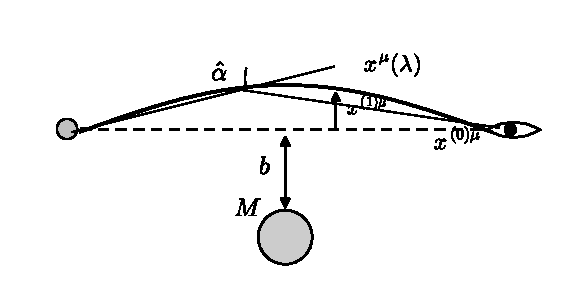
\includegraphics[width=0.72\textwidth]{fig_7.3.pdf}
\caption*{图 7.3\quad 一条被偏折的测地线 $x^{\mu}(\lambda)$，分解为一条背景测地线 $x^{(0)\mu}$ 和一个微扰 $x^{(1)\mu}$。偏转角 $\widehat{\alpha}$ 代表波矢量（wave vector）沿路径转过的量的（负值）。图中画出的是碰撞参数（impact parameter）为 $b$ 的单个质量 $M$，尽管这一设置更具一般性。}
\end{figure}

或等价地
\begin{equation*}
h_{\mu\nu} =
\begin{pmatrix}
-2\Phi & & & \\
& -2\Phi & & \\
& & -2\Phi & \\
& & & -2\Phi
\end{pmatrix},
\tag{7.60}
\end{equation*}
其中势满足通常的 Poisson 方程，
\begin{equation*}
\nabla^2\Phi = 4\pi G\rho.
\tag{7.61}
\end{equation*}
这是对第 4 章结果的一个重要推广，因为我们现在不仅知道 $h_{00}$，还知道空间度规的微扰。

现在让我们考虑光子（或其他无质量粒子）在这个几何中的路径；换句话说，对类光轨迹 $x^\mu(\lambda)$ 求解微扰后的测地线方程。\footnote{我们所用的方法在 T.~Pyne 和 M.~Birkinshaw 的文章 \emph{Astrophys. Journ.} 458, 46 (1996) 中有概述，见 \texttt{http://arxiv.org/abs/astro-ph/9504060}。}我们所考虑的几何描绘于图 7.3。回想一下，我们的处理思路是把度规微扰当作定义在平直背景时空上的场。类似地，我们可以把测地线分解为背景路径加上微扰，
\begin{equation*}
x^\mu(\lambda) = x^{(0)\mu}(\lambda) + x^{(1)\mu}(\lambda),
\tag{7.62}
\end{equation*}
其中 $x^{(0)\mu}$ 满足背景中的测地线方程（换句话说，就是一条笔直的类光路径）。然后我们沿背景路径取所有量的值，来求解 $x^{(1)\mu}(\lambda)$。要让这一做法行得通，我们需要假设势 $\Phi$ 沿背景测地线与真实测地线没有明显差别；这个条件相当于要求 $x^{(1)i}\partial_i\Phi \ll \Phi$。不过，即使这个条件不成立，也并非全盘皆输。如果我们只考虑非常短的路径，偏离

% ---- 书页 289 / p304 ----

$x^{(1)\mu}$ 就必然很小，我们的近似也将有效。而接下来我们可以用这样的短段拼接出更长的路径。结果是，我们会推导出真实的方程，只是积分所沿的路径将是\emph{真实}路径 $x^\mu(\lambda)$，而不是背景路径 $x^{(0)\mu}(\lambda)$。只要理解了这一点，我们的结果对微扰时空中的任何轨迹都将成立。

为方便起见，我们把背景路径的波矢量记作 $k^\mu$，把偏离矢量的导数记作 $\ell^\mu$：
\begin{equation*}
k^\mu \equiv \frac{dx^{(0)\mu}}{d\lambda}, \qquad \ell^\mu \equiv \frac{dx^{(1)\mu}}{d\lambda}.
\tag{7.63}
\end{equation*}
路径为类光的条件当然是
\begin{equation*}
g_{\mu\nu}\frac{dx^\mu}{d\lambda}\frac{dx^\nu}{d\lambda} = 0,
\tag{7.64}
\end{equation*}
我们必须逐阶求解它。零阶时我们直接有 $\eta_{\mu\nu}k^\mu k^\nu = 0$，即
\begin{equation*}
(k^0)^2 = (\vec{k}\,)^2 \equiv k^2,
\tag{7.65}
\end{equation*}
其中 $\vec{k}$ 是分量为 $k^i$ 的三维矢量。这个方程充当常数 $k$ 的定义。于一阶我们得到
\begin{equation*}
2\eta_{\mu\nu}k^\mu\ell^\nu + h_{\mu\nu}k^\mu k^\nu = 0,
\tag{7.66}
\end{equation*}
即
\begin{equation*}
-k\ell^0 + \vec{\ell}\cdot\vec{k} = 2k^2\Phi.
\tag{7.67}
\end{equation*}

现在我们转向微扰后的测地线方程，
\begin{equation*}
\frac{d^2x^\mu}{d\lambda^2} + \Gamma^\mu_{\rho\sigma}\frac{dx^\rho}{d\lambda}\frac{dx^\sigma}{d\lambda} = 0.
\tag{7.68}
\end{equation*}
把 $w^i = 0$ 和 $h_{ij} = -2\Phi\delta_{ij}$ 代入 (7.19)，便可以求出 Christoffel 符号：
\begin{align*}
\Gamma^0_{0i} &= \Gamma^i_{00} = \partial_i\Phi, \\
\Gamma^i_{jk} &= \delta_{jk}\partial_i\Phi - \delta_{ik}\partial_j\Phi - \delta_{ij}\partial_k\Phi.
\tag{7.69}
\end{align*}
零阶测地线方程只是告诉我们 $x^{(0)\mu}$ 是一条直线轨迹，而在一阶我们有
\begin{equation*}
\frac{d\ell^\mu}{d\lambda} = -\Gamma^\mu_{\rho\sigma}k^\rho k^\sigma.
\tag{7.70}
\end{equation*}

% ---- 书页 290 / p305 ----

右端没有 $\ell^\mu$ 的因子，因为 Christoffel 符号已经是微扰的一阶量。(7.70) 的 $\mu = 0$ 分量为
\begin{equation*}
\frac{d\ell^0}{d\lambda} = -2k(\vec{k}\cdot\vec{\nabla}\Phi),
\tag{7.71}
\end{equation*}
而空间分量为
\begin{equation*}
\frac{d\vec{\ell}}{d\lambda} = -2k^2\vec{\nabla}_{\perp}\Phi.
\tag{7.72}
\end{equation*}
这里我们引入了横向于路径的梯度，它定义为总梯度减去沿路径方向的梯度，
\begin{align*}
\vec{\nabla}_{\perp}\Phi &\equiv \vec{\nabla}\Phi - \vec{\nabla}_{\parallel}\Phi \\
&= \vec{\nabla}\Phi - k^{-2}(\vec{k}\cdot\vec{\nabla}\Phi)\vec{k}.
\tag{7.73}
\end{align*}
在以上所有表达式中，路径均指背景路径。

注意，在 $\Phi$ 的一阶精度下，空间波矢量微扰 $\vec{\ell}$ 与原有的空间波矢量 $\vec{k}$ 正交。为看清这一点，我们可以积分 (7.71) 得到 $\ell^0$ 的表达式：
\begin{align*}
\ell^0 &= \int \frac{d\ell^0}{d\lambda}\, d\lambda \\
&= -2k\int (\vec{k}\cdot\vec{\nabla}\Phi)\, d\lambda \\
&= -2k\int \left(\frac{d\vec{x}}{d\lambda}\cdot\vec{\nabla}\Phi\right) d\lambda \\
&= -2k\int \vec{\nabla}\Phi\cdot d\vec{x} \\
&= -2k\Phi.
\tag{7.74}
\end{align*}
积分常数由 $\Phi = 0$ 时 $\ell^0 = 0$ 的要求确定。把它代入 (7.67)，得到
\begin{equation*}
\vec{\ell}\cdot\vec{k} = k\ell^0 + 2k^2\Phi = 0,
\tag{7.75}
\end{equation*}
这就验证了 $\vec{\ell}$ 与 $\vec{k}$ 在一阶精度下正交。

\textbf{偏转角}（deflection angle）$\widehat{\alpha}$ 是原有的空间波矢量从源传播到观者处时被偏折的量；它是垂直于 $\vec{k}$ 的平面内的一个二维矢量。（我们采用记号 $\widehat{\alpha}$ 而不是 $\vec{\alpha}$，因为后者已留给第 8 章引入的约化偏转角（reduced deflection angle）。）由图 7.3 所描绘的几何，偏转角可以表示为

% ---- 书页 291 / p306 ----

\begin{equation*}
\widehat{\alpha} = -\frac{\Delta\vec{\ell}}{k},
\tag{7.76}
\end{equation*}
其中负号只是考虑到这样一个事实：偏转角是由沿光子路径向后看的观者测量的。波矢量的转动可以由 (7.72) 算出：
\begin{align*}
\Delta\vec{\ell} &= \int\frac{d\vec{\ell}}{d\lambda}\, d\lambda \\
&= -2k^2\int \vec{\nabla}_{\perp}\Phi\, d\lambda.
\tag{7.77}
\end{align*}
因此，偏转角可以写成沿所经过的物理空间距离 $s = k\lambda$ 的积分：
\begin{equation*}
\boxed{\,\widehat{\alpha} = 2\int \vec{\nabla}_{\perp}\Phi\, ds.\,}
\tag{7.78}
\end{equation*}

我们可以在点质量的情形下算出偏转角：设想背景路径沿 $x$ 方向，碰撞参数由一个横向矢量 $\vec{b}$ 定义，它在最接近点处从路径指向质量。取 $b = |\vec{b}|$，势为
\begin{equation*}
\Phi = -\frac{GM}{r} = -\frac{GM}{(b^2+x^2)^{1/2}},
\tag{7.79}
\end{equation*}
其横向梯度因此为
\begin{equation*}
\vec{\nabla}_{\perp}\Phi = \frac{GM}{(b^2+x^2)^{3/2}}\vec{b}.
\tag{7.80}
\end{equation*}
于是偏转角为
\begin{align*}
\widehat{\alpha} &= 2GMb\int \frac{dx}{(b^2+x^2)^{3/2}} \\
&= \frac{4GM}{b},
\tag{7.81}
\end{align*}
其中积分取自 $-\infty$ 到 $\infty$，这里假定了源和观者都离偏折质量非常远。注意在我们的单位制中 $c = 1$；在其他单位制下，应在 (7.81) 的分母中补上因子 $c^2$。

太阳对光的偏折在历史上是广义相对论的一个关键检验。Einstein 提出了三项这样的检验：水星近日点进动、引力红移和光线偏折。水星近日点进动被 GR 成功解释，但它解释的是一个早已被观测到的偏差；引力红移直到很久之后才被观测到，
% ---- 书页 292 / p307 ----
因此光线偏折是 Einstein 的理论第一次正确预言了尚未被探测到的现象。Eddington 率领的一支著名远征队在 1919 年的日全食期间观测了太阳附近恒星的位置；观测结果与 GR 预言相符，世界各地的报纸都在头版报道了这一消息。预言的效应相当小：对太阳而言，$GM_\odot/c^2 = 1.48\times10^5$ cm，太阳半径为 $R_\odot = 6.96\times10^{10}$ cm，由此给出的最大偏转角为 $\widehat{\alpha} = 1.75$ 角秒。后来对 Eddington 结果的重新评估使人们怀疑他是否真的达到了当初宣称的精度；当代的测量则利用从太阳背后经过的类星体（quasar）的高精度干涉观测，对 GR 作出非常精确的检验（GR 迄今为止都经受了这些检验）。与此同时，对星系和恒星等天体物理源造成的光线偏折的观测，已经发展成一个活跃的研究领域，其名目叫作“引力透镜”。当然，在这种情形下我们对透镜质量的了解很少能达到为 GR 提供精密检验的程度；更常见的做法反而是把观测到的偏转角用作测量质量的一种手段。我们将在第 8 章进一步讨论透镜。

除了光线偏折之外，1964 年 Shapiro 还指出了弱场广义相对论在光子轨迹上的另一个可观测结果：引力时间延迟（gravitational time delay）。沿一条类光路径所耗费的坐标时间为
\begin{equation*}
t = \int\frac{dx^0}{d\lambda}\, d\lambda.
\tag{7.82}
\end{equation*}
我们把自己放在一个远离一切源、静止于背景惯性系中的观者的位置上，因此坐标时间就是我们的固有时。在存在 Newton 势的情况下，光子相对于背景光锥看起来“慢了下来”，由此导致的附加时间延迟为
\begin{align*}
\Delta t &= \int\frac{dx^{(1)0}}{d\lambda}\, d\lambda \\
&= \int \ell^0\, d\lambda \\
&= -2k\int \Phi\, d\lambda,
\tag{7.83}
\end{align*}
即
\begin{equation*}
\Delta t = -2\int \Phi\, ds.
\tag{7.84}
\end{equation*}

按照我们的规则，积分沿背景路径进行。除了这个 Shapiro 延迟之外，还可能有一个额外的“几何”时间延迟，因为真实路径经过的空间距离比背景路径更长。对太阳造成的光线偏折而言，几何延迟效应可以忽略，但在宇宙学的应用中，
% ---- 书页 293 / p308 ----
它可以与 Shapiro 效应相比拟。这一时间延迟已被观测到，其中最精确的测量利用的是航天器而非天然天体；详见 Will (1981)。

光子穿过 Newton 势的运动——它同时导致光线偏折和引力时间延迟——也可以等价地这样导出：设想光子是在折射率（refractive index）为
\begin{equation*}
n = 1 - 2\Phi,
\tag{7.85}
\end{equation*}
的介质中传播（精确到一阶）。事实上，我们本可以利用 Fermat 最短时间原理（Fermat's principle of least time）求出光子的运动方程；习题中将请你证明这一点。

\section{引力波解}

弱场极限一个更令人兴奋的应用是引力辐射。这里我们研究的是引力场的自由传播自由度，它们的存在不需要任何局域的源（当然它们可以由这类源产生）。于是我们再一次回到横向规范下的弱场方程，即式 (7.38)--(7.40)，但这一次保留时间导数，同时完全关掉能量-动量张量，$T_{\mu\nu} = 0$。这时 00 方程为
\begin{equation*}
\nabla^2\Psi = 0,
\tag{7.86}
\end{equation*}
在表现良好的边界条件下，这意味着 $\Psi = 0$。于是 $0j$ 方程为
\begin{equation*}
\nabla^2 w_j = 0,
\tag{7.87}
\end{equation*}
这同样意味着 $w_j = 0$。

接下来看 $ij$ 方程的迹，（代入上面的结果后）它给出
\begin{equation*}
\nabla^2\Phi = 0,
\tag{7.88}
\end{equation*}
这意味着 $\Phi = 0$。

于是只剩下 $ij$ 方程的无迹部分，它成为无迹应变张量（strain tensor）的波动方程：
\begin{equation*}
\Box s_{ij} = 0.
\tag{7.89}
\end{equation*}
虽然到目前为止用 $s_{ij}$ 做事很方便，但文献中远为常见的做法是用整个度规微扰 $h_{\mu\nu}$ 来书写表达式，不过采用的拟设是令所有其他自由度 $(\Phi, \Psi, w_i)$ 都为零（且 $s_{ij}$ 是横向的）。这就是通常所说的\textbf{横无迹（TT）规范}（transverse-traceless gauge），其中有

% ---- 书页 294 / p309 ----

\begin{equation*}
h^{\mathrm{TT}}_{\mu\nu} =
\begin{pmatrix}
0 & 0 & 0 & 0 \\
0 & & & \\
0 & & 2s_{ij} & \\
0 & & &
\end{pmatrix}.
\tag{7.90}
\end{equation*}
这时的运动方程为
\begin{equation*}
\Box h^{\mathrm{TT}}_{\mu\nu} = 0.
\tag{7.91}
\end{equation*}
为了更容易与其他资料对照，在讨论引力波时我们将使用 $h^{\mathrm{TT}}_{\mu\nu}$ 而不是 $s_{ij}$，同时记住 $h^{\mathrm{TT}}_{\mu\nu}$ 是纯空间的、无迹且横向的：
\begin{gather*}
h^{\mathrm{TT}}_{0\nu} = 0 \\
\eta^{\mu\nu}h^{\mathrm{TT}}_{\mu\nu} = 0 \\
\partial_\mu h^{\mu\nu}_{\mathrm{TT}} = 0.
\tag{7.92}
\end{gather*}

我们从波动方程 (7.91) 出发寻找解。熟悉电磁学中类似问题的读者会注意到，这里的步骤几乎一模一样。这族波动方程中特别有用的一组解是平面波，由下式给出
\begin{equation*}
h^{\mathrm{TT}}_{\mu\nu} = C_{\mu\nu}e^{ik_\sigma x^\sigma},
\tag{7.93}
\end{equation*}
其中 $C_{\mu\nu}$ 是一个常值、对称的 $(0,2)$ 型张量，显然无迹且纯空间：
\begin{gather*}
C_{0\nu} = 0 \\
\eta^{\mu\nu}C_{\mu\nu} = 0.
\tag{7.94}
\end{gather*}
当然，$e^{ik_\sigma x^\sigma}$ 是复的，而 $h^{\mathrm{TT}}_{\mu\nu}$ 是实的；我们让实部和虚部一起贯穿整个计算，最后再取实部。常矢量 $k^\sigma$ 就是波矢量。为了确认我们得到的确是一个解，把它代入：
\begin{align*}
0 &= \Box h^{\mathrm{TT}}_{\mu\nu} \\
&= \eta^{\rho\sigma}\partial_\rho\partial_\sigma h^{\mathrm{TT}}_{\mu\nu} \\
&= \eta^{\rho\sigma}\partial_\rho(ik_\sigma h^{\mathrm{TT}}_{\mu\nu}) \\
&= -\eta^{\rho\sigma}k_\rho k_\sigma h^{\mathrm{TT}}_{\mu\nu} \\
&= -k_\sigma k^\sigma h^{\mathrm{TT}}_{\mu\nu}.
\tag{7.95}
\end{align*}

% ---- 书页 295 / p310 ----

由于对一个有意义的解来说，$h^{\mathrm{TT}}_{\mu\nu}$ 的各分量不会处处都为零，我们必须有
\begin{equation*}
k_\sigma k^\sigma = 0.
\tag{7.96}
\end{equation*}
因此，只要波矢量是类光的，平面波 (7.93) 就是线性化方程的解；这可以粗略地转述为：引力波以光速传播。波矢量的类时分量就是波的频率，我们把它写作 $k^\sigma = (\omega, k^1, k^2, k^3)$。（更一般地，以四速度 $U^\mu$ 运动的观者会观测到波的频率为 $\omega = -k_\mu U^\mu$。）于是波矢量为类光的条件就成为
\begin{equation*}
\omega^2 = \delta_{ij}k^ik^j.
\tag{7.97}
\end{equation*}

当然，我们的波远非最一般的解；任意（可能无限多个）不同的平面波可以相加，而且仍然求解线性方程 (7.91)。事实上，任何解都可以写成这样的叠加。

我们还需要保证微扰是横向的。这意味着
\begin{align*}
0 &= \partial_\mu h^{\mu\nu}_{\mathrm{TT}} \\
&= iC^{\mu\nu}k_\mu e^{ik_\sigma x^\sigma},
\tag{7.98}
\end{align*}
而这只有当
\begin{equation*}
k_\mu C^{\mu\nu} = 0.
\tag{7.99}
\end{equation*}
时才成立。我们说波矢量与 $C^{\mu\nu}$ 正交。

选取空间坐标使波沿 $x^3$ 方向传播，可以把我们的解写得更显式；也就是说，
\begin{equation*}
k^\mu = (\omega, 0, 0, k^3) = (\omega, 0, 0, \omega),
\tag{7.100}
\end{equation*}
其中我们知道 $k^3 = \omega$，因为波矢量是类光的。在这种情形下，$k^\mu C_{\mu\nu} = 0$ 与 $C_{0\nu} = 0$ 合起来意味着
\begin{equation*}
C_{3\nu} = 0.
\tag{7.101}
\end{equation*}
于是 $C_{\mu\nu}$ 仅有的非零分量是 $C_{11}$、$C_{12}$、$C_{21}$ 和 $C_{22}$。但 $C_{\mu\nu}$ 无迹且对称，故一般地可以写成
\begin{equation*}
C_{\mu\nu} =
\begin{pmatrix}
0 & 0 & 0 & 0 \\
0 & C_{11} & C_{12} & 0 \\
0 & C_{12} & -C_{11} & 0 \\
0 & 0 & 0 & 0
\end{pmatrix}.
\tag{7.102}
\end{equation*}
这样，对这个规范中沿 $x^3$ 方向传播的平面波，两个分量 $C_{11}$ 和 $C_{12}$（连同频率 $\omega$）就完全刻画了这个波。

% ---- 书页 296 / p311 ----

为了体会引力波经过时的物理效应，考虑检验粒子在波存在时的运动。只求解单个粒子的轨迹肯定是不够的，因为那只会告诉我们世界线上坐标的取值。事实上，对任何一个单独的粒子，我们都能找到一组横无迹坐标（transverse traceless coordinates），使这个粒子在精确到 $h^{\mathrm{TT}}_{\mu\nu}$ 一阶的意义下显得静止。为了得到一个不依赖坐标的量来量度波的效应，我们考虑邻近粒子的相对运动，这由测地偏离方程描述。如果考虑一些邻近的粒子，其四速度由同一个矢量场 $U^\mu(x)$ 描写，间隔矢量为 $S^\mu$，则有
\begin{equation*}
\frac{D^2}{d\tau^2}S^\mu = R^\mu{}_{\nu\rho\sigma}U^\nu U^\rho S^\sigma.
\tag{7.103}
\end{equation*}
我们希望把右端计算到 $h^{\mathrm{TT}}_{\mu\nu}$ 的一阶。如果取检验粒子缓慢运动，我们可以把四速度表成时间方向的单位矢量加上 $h^{\mathrm{TT}}_{\mu\nu}$ 阶及更高阶的改正；但我们知道 Riemann 张量已经是一阶量，所以 $U^\nu$ 的改正可以忽略，于是写成
\begin{equation*}
U^\nu = (1, 0, 0, 0).
\tag{7.104}
\end{equation*}
因此我们只需计算 $R^\mu{}_{00\sigma}$，或等价地 $R_{\mu 00\sigma}$。由 (7.5) 有
\begin{equation*}
R_{\mu 00\sigma} = \tfrac{1}{2}(\partial_0\partial_0 h^{\mathrm{TT}}_{\mu\sigma} + \partial_\sigma\partial_\mu h^{\mathrm{TT}}_{00} - \partial_\sigma\partial_0 h^{\mathrm{TT}}_{\mu 0} - \partial_\mu\partial_0 h^{\mathrm{TT}}_{\sigma 0}).
\tag{7.105}
\end{equation*}
但 $h^{\mathrm{TT}}_{\mu 0} = 0$，所以
\begin{equation*}
R_{\mu 00\sigma} = \tfrac{1}{2}\partial_0\partial_0 h^{\mathrm{TT}}_{\mu\sigma}.
\tag{7.106}
\end{equation*}
另一方面，对缓慢运动的粒子，在最低阶我们有 $\tau = x^0 = t$，于是测地偏离方程成为
\begin{equation*}
\frac{\partial^2}{\partial t^2}S^\mu = \frac{1}{2}S^\sigma\frac{\partial^2}{\partial t^2}h^{\mathrm{TT}\mu}{}_{\sigma}.
\tag{7.107}
\end{equation*}

对我们的沿 $x^3$ 方向传播的波，这意味着只有 $S^1$ 和 $S^2$ 会受到影响——检验粒子只在垂直于波矢量的方向上被扰动。这一点在电磁学中是大家熟悉的：平面波中的电场和磁场都垂直于波矢量。

我们的波由这两个数刻画，为了后面方便，我们把它们重新命名为：
\begin{gather*}
h_+ = C_{11} \\
h_\times = C_{12},
\tag{7.108}
\end{gather*}

% ---- 书页 297 / p312 ----

于是
\begin{equation*}
C_{\mu\nu} =
\begin{pmatrix}
0 & 0 & 0 & 0 \\
0 & h_+ & h_\times & 0 \\
0 & h_\times & -h_+ & 0 \\
0 & 0 & 0 & 0
\end{pmatrix}.
\tag{7.109}
\end{equation*}
让我们分别考虑二者的效应，先讨论 $h_\times = 0$ 的情形。这时有
\begin{equation*}
\frac{\partial^2}{\partial t^2}S^1 = \frac{1}{2}S^1\frac{\partial^2}{\partial t^2}(h_+e^{ik_\sigma x^\sigma})
\tag{7.110}
\end{equation*}
而
\begin{equation*}
\frac{\partial^2}{\partial t^2}S^2 = -\frac{1}{2}S^2\frac{\partial^2}{\partial t^2}(h_+e^{ik_\sigma x^\sigma}).
\tag{7.111}
\end{equation*}
这两个方程可以立即解出，在最低阶给出
\begin{equation*}
S^1 = \left(1 + \tfrac{1}{2}h_+e^{ik_\sigma x^\sigma}\right)S^{1}{}_{(0)}
\tag{7.112}
\end{equation*}
以及
\begin{equation*}
S^2 = \left(1 - \tfrac{1}{2}h_+e^{ik_\sigma x^\sigma}\right)S^{2}{}_{(0)}.
\tag{7.113}
\end{equation*}

于是，初始时刻沿 $x^1$ 方向分开的粒子将在 $x^1$ 方向上振荡，初始沿 $x^2$ 方向分开的粒子亦然。也就是说，如果我们从 $x$-$y$ 平面上一圈静止的粒子出发，那么当波经过时，它们会以“+”的形状来回弹动，如图 7.4 所示。另一方面，对 $h_+ = 0$ 而 $h_\times \neq 0$ 的情形作同样的分析，将得到解
\begin{equation*}
S^1 = S^{1}{}_{(0)} + \tfrac{1}{2}h_\times e^{ik_\sigma x^\sigma}S^{2}{}_{(0)}
\tag{7.114}
\end{equation*}
以及
\begin{equation*}
S^2 = S^{2}{}_{(0)} + \tfrac{1}{2}h_\times e^{ik_\sigma x^\sigma}S^{1}{}_{(0)}.
\tag{7.115}
\end{equation*}

\begin{figure}[H]
\centering
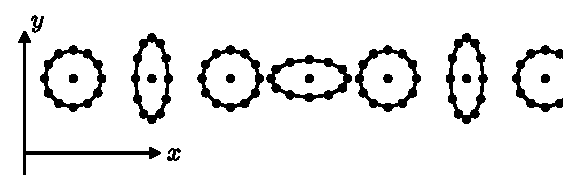
\includegraphics[width=0.72\textwidth]{fig_7.4.pdf}
\caption*{图 7.4\quad 具有 + 偏振的引力波会把检验粒子圆环扭曲成按 + 图样振荡的椭圆。}
\end{figure}

% ---- 书页 298 / p313 ----

\begin{figure}[H]
\centering
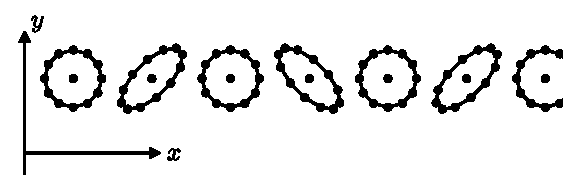
\includegraphics[width=0.72\textwidth]{fig_7.5.pdf}
\caption*{图 7.5\quad 具有 $\times$ 偏振的引力波会把检验粒子圆环扭曲成按 $\times$ 图样振荡的椭圆。}
\end{figure}

在这种情形下，粒子圆环会来回弹动，保持“$\times$”的形状，如图 7.5 所示。因此 $h_+$ 和 $h_\times$ 这两个记号的含义应当清楚了。这两个量量度引力波的两种独立的线偏振模式，分别称为“+”偏振与“$\times$”偏振（plus and cross）。如果我们愿意，通过定义
\begin{gather*}
h_R = \frac{1}{\sqrt{2}}(h_+ + ih_\times), \\
h_L = \frac{1}{\sqrt{2}}(h_+ - ih_\times).
\tag{7.116}
\end{gather*}
就可以考虑右旋和左旋的圆偏振模式。

一个纯 $h_R$ 波的效应是使粒子沿右手方向转动，如图 7.6 所示；左旋模式 $h_L$ 与此类似。注意，各个粒子并不绕着环运动；它们只是在小本轮（epicycles）上打转。

我们可以把经典引力波的偏振态与量子化后预期会出现的粒子种类联系起来。量子化场的自旋与该场在空间转动下的变换性质直接相关。电磁场有两个独立的偏振态，由 $x$-$y$ 平面内的矢量描写；等价地说，单一偏振模式在这个平面内转动 $360^{\circ}$ 后保持不变。量子化后，这个理论给出光子——一种无质量的自旋为 1 的粒子。而中微子也是一种无质量粒子，描写它的场在转动 $360^{\circ}$ 下改变符号；它在 $720^{\circ}$ 转动下不变，于是我们说它具有

\begin{figure}[H]
\centering
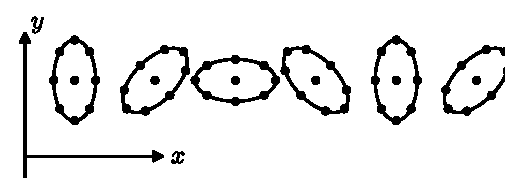
\includegraphics[width=0.72\textwidth]{fig_7.6.pdf}
\caption*{图 7.6\quad 具有 R 偏振的引力波会把检验粒子圆环扭曲成沿右手方向旋转的椭圆。}
\end{figure}
自旋 $1/2$。一般的规律是：自旋 $S$ 与偏振模式在转动下保持不变所对应的角 $\theta$ 之间的关系为 $S = 360^{\circ}/\theta$。引力场——它的波以光速传播——在量子理论中应当导致无质量粒子。注意到我们所描述的偏振模式在 $x$-$y$ 平面内转动 $180^{\circ}$ 下不变，我们预期相应的粒子——引力子（gravitons）——是自旋 2 的。探测这样的粒子还遥遥无期（就算我们永远无法直接探测到它们，也不会令人惊讶），但任何一门像样的引力量子理论都应当预言它们的存在。

% ---- 书页 299 / p314 ----（本页第一段已在上面 tail 中接续，正文自第二段起）

事实上，从自旋为 2 的引力子理论出发，再加上一些简单性质的要求，就为\emph{导出}广义相对论完整的 Einstein 方程提供了一条漂亮的途径。设想从对称张量 $h_{\mu\nu}$ 的拉格朗日量 (7.9) 出发，但现在设想这个场“其实真的是”一个在 Minkowski 时空中传播的物理场，而不是动力学度规上的微扰。（这个拉格朗日量不包含与物质的耦合，不过把它加上并不困难。）现在再追加一条要求：让 $h_{\mu\nu}$ 与它自身的能量-动量张量（下文讨论）耦合，同时也与物质的能量-动量张量耦合。这会在作用量中诱导出高阶非线性项，随之又诱导出阶数更高的“能量-动量”项。反复重复这一过程，就会引入一个无穷多项的级数，但这个级数可以求和成一个简单的表达式——也许是因为你已经知道答案——即 Einstein--Hilbert 作用量（可能还带有一些高阶项）。在这一过程中我们发现，物质与唯一的组合 $g_{\mu\nu} = \eta_{\mu\nu} + h_{\mu\nu}$ 耦合。换句话说，仅仅要求一个自旋为 2 的场与能量-动量张量耦合，我们最终就得到了广义相对论完全非线性的全部辉煌。背景度规 $\eta_{\mu\nu}$ 变得完全不可观测。当然，广义相对论的某些整体几何面貌被这套程序掩盖了；它归根结底只是为 Einstein 方程提供论证的另一种方式。

在我们谈论这些趣事之际，不妨指出：引力波的行为为弦论为何会给出引力的量子理论提供了一条线索。考虑一根弦圈的基本振动模式，如图 7.7 所示。一根弦圈有三个能量最低的模式：

% ---- 书页 300 / p315 ----（承接上页段末"……三个能量最低的模式："）

一个整体的大小振荡，外加两种独立的、振荡成椭圆的方式。它们给出三个无质量自由度：一个自旋为 0 的粒子（伸缩子，dilaton）和一个无质量的自旋为 2 的粒子（引力子）。注意弦的振荡与检验粒子在引力波影响下的运动之间有着明显的相似；这绝非偶然，这正是量子化的弦不可避免地给出引力的原因。（弦论最初是作为强相互作用理论被研究的，但各种模型都不可避免地预言一个多余的无质量自旋 2 粒子；人们最终意识到，如果把这个理论当作引力的量子理论来看待，这个缺陷反而可以变成优点。）那个多余而无用的自旋 0（标量）模式反映了这样的事实：弦论实际上预言的是一个标量-张量引力理论（如 4.8 节所讨论），而不是普通的广义相对论。由于自然界中并没有观察到这种无质量标量，必定要有某种机制在低能下赋予这个标量质量。

\begin{figure}[H]
\centering
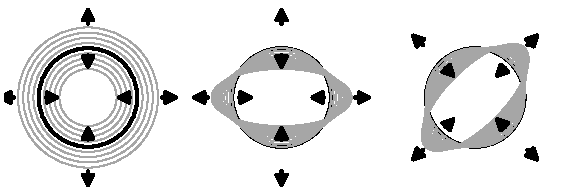
\includegraphics[width=0.72\textwidth]{fig_7.7.pdf}
\caption*{图 7.7\quad 一根弦圈的三个基本振动模式。整体的"呼吸"模式（最左）在转动下不变，给出一个自旋为 0 的粒子。另外两个模式与引力波的两个偏振相匹配，代表一个无质量自旋 2 粒子的两个态。}
\end{figure}

\section{引力波的产生}

有了线性化真空方程的平面波解，剩下要讨论的就是源对引力辐射的产生。为此有必要考虑与物质耦合的 Einstein 方程 $G_{\mu\nu} = 8\pi G T_{\mu\nu}$。由于 $T_{\mu\nu}$ 不为零，度规微扰除了表示引力波的应变张量之外，还将包含非零的标量和矢量分量；我们不能假定解取横无迹形式 (7.90)。相反，我们将保留完整的微扰 $h_{\mu\nu}$，求出在远离源处产生的引力波，在那里我们随后可以施加横无迹规范。

即便有源存在，我们仍然可以引入一些方便的简化。首先定义无迹反转微扰（trace-reversed perturbation），
\begin{equation*}
\bar{h}_{\mu\nu} = h_{\mu\nu} - \frac{1}{2}\eta_{\mu\nu}h.
\tag{7.117}
\end{equation*}
“无迹反转微扰”这个名字是有道理的，因为
\begin{equation*}
\bar{h} = \eta^{\mu\nu}\bar{h}_{\mu\nu} = -h.
\tag{7.118}
\end{equation*}
显然，我们可以从无迹反转形式重构出原来的微扰，因此没有丢失任何信息。还要注意，如果我们在远离任何源的真空区域、并且可以取横无迹规范，那么无迹反转微扰将等于原来的微扰，
\begin{equation*}
\bar{h}^{\mathrm{TT}}_{\mu\nu} = h^{\mathrm{TT}}_{\mu\nu}.
\tag{7.119}
\end{equation*}
同时，我们仍然可以自由选择某种规范。在规范变换 (7.14) 下，无迹反转微扰按下式变换：
\begin{equation*}
\bar{h}_{\mu\nu} \rightarrow \bar{h}_{\mu\nu} + 2\partial_{(\mu}\xi_{\nu)} - \partial_\lambda\xi^{\lambda}\eta_{\mu\nu}.
\tag{7.120}
\end{equation*}

% ---- 书页 301 / p316 ----

于是，通过选取满足
\begin{equation*}
\Box\xi_\mu = -\partial_\lambda\bar{h}^{\lambda}{}_{\mu},
\tag{7.121}
\end{equation*}
的规范参数 $\xi_\mu$，我们就可以令
\begin{equation*}
\partial_\mu\bar{h}^{\mu\nu} = 0.
\tag{7.122}
\end{equation*}
这个条件称为\textbf{Lorenz 规范}，与电磁学中经常使用的类似条件 $\partial_\mu A^\mu = 0$ 相仿。\footnote{注意拼写。这个“规范”（gauge）源自 Ludwig Lorenz（1829--1891），而更有名的“变换”（transformation）则由 Hendrick Antoon Lorentz（1853--1928）发明。参见 J.~D. Jackson 和 L.~B. Okun，\emph{Rev. Mod. Phys.} 73, 663 (2001)。}注意，原来的微扰在这个规范下并不是横向的；确切地说，我们有
\begin{equation*}
\partial_\mu h^{\mu\nu} = \frac{1}{2}\partial^\nu h.
\tag{7.123}
\end{equation*}
把无迹反转微扰的定义代入我们的 Einstein 张量表达式 (7.8)，并利用 Lorenz 规范条件，便得到一个非常简洁的表达式
\begin{equation*}
G_{\mu\nu} = -\frac{1}{2}\Box\bar{h}_{\mu\nu}.
\tag{7.124}
\end{equation*}
用原来的微扰 $h_{\mu\nu}$ 写出的相应表达式则要稍微杂乱一些；这正是引入 $\bar{h}_{\mu\nu}$ 的原因。于是，这个规范下的线性化 Einstein 方程就是每个分量各自满足的一个波动方程，
\begin{equation*}
\Box\bar{h}_{\mu\nu} = -16\pi G T_{\mu\nu}.
\tag{7.125}
\end{equation*}
这类方程的解可以用 Green 函数求得，处理方式与电磁学中的类似问题完全相同。这里我们将循着 Wald (1984) 的路子回顾一下方法的梗概。

d'Alembert 算符 $\Box$ 的 Green 函数 $G(x^\sigma - y^\sigma)$，是波动方程在存在 $\delta$ 函数源时的解：
\begin{equation*}
\Box_x G(x^\sigma - y^\sigma) = \delta^{(4)}(x^\sigma - y^\sigma),
\tag{7.126}
\end{equation*}
其中 $\Box_x$ 表示对坐标 $x^\sigma$ 的 d'Alembert 算符。这类函数的用处在于，诸如 (7.125) 这样的方程的一般解可以写成
\begin{equation*}
\bar{h}_{\mu\nu}(x^\sigma) = -16\pi G\int G(x^\sigma - y^\sigma)T_{\mu\nu}(y^\sigma)\, d^{4}y,
\tag{7.127}
\end{equation*}
这可以立即得到验证。（注意，不需要任何 $\sqrt{-g}$ 因子，因为我们的背景就是简单的平直时空。）(7.126) 的解当然早就被算出来了，它们可以被视为“推迟的”（retarded）或“超前的”（advanced），取决于它们代表的是在时间中向前还是

% ---- 书页 302 / p317 ----（承接上页段末"……向前还是"）

向后传播的波。我们感兴趣的是推迟 Green 函数，它代表来自所考虑点之过去的信号的累积效应。它由下式给出
\begin{equation*}
G(x^\sigma - y^\sigma) = -\frac{1}{4\pi|\mathbf{x}-\mathbf{y}|}\,\delta\!\left[|\mathbf{x}-\mathbf{y}| - (x^{0} - y^{0})\right]\theta(x^{0} - y^{0}).
\tag{7.128}
\end{equation*}
这里我们已经用粗体表示空间矢量 $\mathbf{x} = (x^{1}, x^{2}, x^{3})$ 和 $\mathbf{y} = (y^{1}, y^{2}, y^{3})$，其模为 $|\mathbf{x}-\mathbf{y}| = [\delta_{ij}(x^{i}-y^{i})(x^{j}-y^{j})]^{1/2}$。$\theta$ 函数 $\theta(x^{0}-y^{0})$ 在 $x^{0} > y^{0}$ 时等于 1，否则为零。(7.128) 的推导会使我们离题太远，但在任何一本关于电动力学或物理中的偏微分方程的标准教科书中都可以找到。

把 (7.128) 代入 (7.127)，我们可以利用 $\delta$ 函数完成对 $y^{0}$ 的积分，得到
\begin{equation*}
\bar{h}_{\mu\nu}(t, \mathbf{x}) = 4G\int \frac{1}{|\mathbf{x}-\mathbf{y}|}T_{\mu\nu}(t - |\mathbf{x}-\mathbf{y}|, \mathbf{y})\, d^{3}y,
\tag{7.129}
\end{equation*}
其中 $t = x^{0}$。“推迟时间”（retarded time）一词指的正是量
\begin{equation*}
t_r = t - |\mathbf{x}-\mathbf{y}|.
\tag{7.130}
\end{equation*}
(7.129) 的含义应当是清楚的：引力场在 $(t, \mathbf{x})$ 处的扰动，是过去光锥上的点 $(t_r, \mathbf{x}-\mathbf{y})$ 处的能量与动量源的影响之总和，如图 7.8 所描绘。

\begin{figure}[H]
\centering
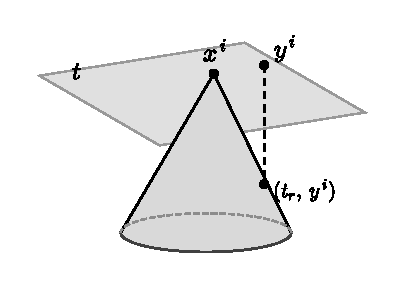
\includegraphics[width=0.72\textwidth]{fig_7.8.pdf}
\caption*{图 7.8\quad 引力场在 $(t, x^i)$ 处的扰动用过去光锥上的事件来计算。}
\end{figure}

让我们取这个一般解，考虑引力辐射由一个相当遥远的、由非相对论性物质组成的孤立源发出的情形；随着讨论的推进，这些近似会得到更精确的表述。首先我们需要建立几条傅里叶变换的约定，在处理振荡现象时它们总能让我们省力不少。给定一个时空函数 $\phi(t, \mathbf{x})$，我们关心的是它仅对时间的傅里叶变换（及其逆变换），

% ---- 书页 303 / p318 ----

\begin{gather*}
\widetilde{\phi}(\omega, \mathbf{x}) = \frac{1}{\sqrt{2\pi}}\int dt\, e^{i\omega t}\phi(t, \mathbf{x}), \\
\phi(t, \mathbf{x}) = \frac{1}{\sqrt{2\pi}}\int d\omega\, e^{-i\omega t}\widetilde{\phi}(\omega, \mathbf{x}).
\tag{7.131}
\end{gather*}
对度规微扰作变换，我们得到
\begin{align*}
\widetilde{\bar{h}}_{\mu\nu}(\omega, \mathbf{x}) &= \frac{1}{\sqrt{2\pi}}\int dt\, e^{i\omega t}\bar{h}_{\mu\nu}(t, \mathbf{x}) \\
&= \frac{4G}{\sqrt{2\pi}}\int dt\, d^{3}y\, e^{i\omega t}\frac{T_{\mu\nu}(t - |\mathbf{x}-\mathbf{y}|, \mathbf{y})}{|\mathbf{x}-\mathbf{y}|} \\
&= \frac{4G}{\sqrt{2\pi}}\int dt_r\, d^{3}y\, e^{i\omega t_r}e^{i\omega|\mathbf{x}-\mathbf{y}|}\frac{T_{\mu\nu}(t_r, \mathbf{y})}{|\mathbf{x}-\mathbf{y}|} \\
&= 4G\int d^{3}y\, e^{i\omega|\mathbf{x}-\mathbf{y}|}\frac{\widetilde{T}_{\mu\nu}(\omega, \mathbf{y})}{|\mathbf{x}-\mathbf{y}|}.
\tag{7.132}
\end{align*}
在这一串式子中，第一个等式就是傅里叶变换的定义，第二行来自解 (7.129)，第三行是从 $t$ 到 $t_r$ 的变量代换，第四行则又是傅里叶变换的定义。

现在我们作如下近似：源是孤立的、遥远的，并且缓慢运动。这意味着我们可以把源看作中心位于（空间）距离 $r$ 处，源的不同部分位于距离 $r + \delta r$ 处，且 $\delta r \ll r$，如图 7.9 所示。由于源缓慢运动，发射的辐射其频率 $\omega$ 大都足够低，使得 $\delta r \ll \omega^{-1}$。（本质上，光穿越源的速度远远快于源自身各部分的速度。）在这些近似下，$e^{i\omega|\mathbf{x}-\mathbf{y}|}/|\mathbf{x}-\mathbf{y}|$ 这一项可以用 $e^{i\omega r}/r$ 代替，并移到积分号外。这剩下
\begin{equation*}
\widetilde{\bar{h}}_{\mu\nu}(\omega, \mathbf{x}) = 4G\frac{e^{i\omega r}}{r}\int d^{3}y\, \widetilde{T}_{\mu\nu}(\omega, \mathbf{y}).
\tag{7.133}
\end{equation*}

\begin{figure}[H]
\centering
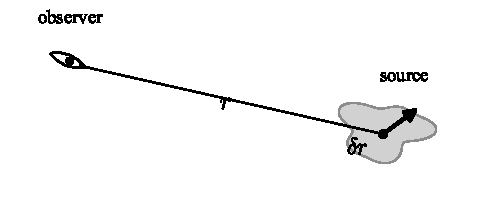
\includegraphics[width=0.72\textwidth]{fig_7.9.pdf}
\caption*{图 7.9\quad 一个尺寸为 $\delta r$ 的源，位于距观者 $r$ 处。}
\end{figure}

% ---- 书页 304 / p319 ----

事实上，我们无须计算 $\widetilde{\bar{h}}_{\mu\nu}(\omega, \mathbf{x})$ 的所有分量，因为 Lorenz 规范条件 $\partial_\mu\bar{h}^{\mu\nu}(t, \mathbf{x}) = 0$ 在傅里叶空间中意味着
\begin{equation*}
\widetilde{\bar{h}}^{0\nu} = \frac{i}{\omega}\partial_i\widetilde{\bar{h}}^{i\nu}.
\tag{7.134}
\end{equation*}
因此我们只需关心 $\widetilde{\bar{h}}_{\mu\nu}(\omega, \mathbf{x})$ 的类空分量，然后再由 (7.134) 恢复出 $\widetilde{\bar{h}}^{0\nu}$。要做的第一件事是令 $\nu = j$，从 $\widetilde{\bar{h}}^{ij}$ 求出 $\widetilde{\bar{h}}^{0j}$，然后再用它从 $\widetilde{\bar{h}}^{i0}$ 求出 $\widetilde{\bar{h}}^{00}$。于是，根据 (7.133)，我们要对 $\widetilde{T}_{\mu\nu}(\omega, \mathbf{y})$ 的类空分量取积分。我们从反向分部积分开始：
\begin{equation*}
\int d^{3}y\, \widetilde{T}^{ij}(\omega, \mathbf{y}) = \int \partial_k(y^{i}\widetilde{T}^{kj})\, d^{3}y - \int y^{i}(\partial_k\widetilde{T}^{kj})\, d^{3}y.
\tag{7.135}
\end{equation*}
第一项是一个面积分，由于源是孤立的，它将消失；第二项则可以通过 $\partial_\mu T^{\mu\nu} = 0$ 的傅里叶空间版本与 $\widetilde{T}^{0j}$ 联系起来：
\begin{equation*}
-\partial_k\widetilde{T}^{k\mu} = i\omega\widetilde{T}^{0\mu}.
\tag{7.136}
\end{equation*}
于是，
\begin{align*}
\int d^{3}y\, \widetilde{T}^{ij}(\omega, \mathbf{y}) &= i\omega\int y^{i}\widetilde{T}^{0j}\, d^{3}y \\
&= \frac{i\omega}{2}\int (y^{i}\widetilde{T}^{0j} + y^{j}\widetilde{T}^{0i})\, d^{3}y \\
&= \frac{i\omega}{2}\int \left[\partial_l(y^{i}y^{j}\widetilde{T}^{0l}) - y^{i}y^{j}(\partial_l\widetilde{T}^{0l})\right] d^{3}y \\
&= -\frac{\omega^{2}}{2}\int y^{i}y^{j}\widetilde{T}^{00}\, d^{3}y.
\tag{7.137}
\end{align*}
第二行的依据是，我们知道左边在 $i$ 和 $j$ 上是对称的；而第三行和第四行不过是把反向分部积分和 $T^{\mu\nu}$ 守恒重复了一遍。习惯上定义源能量密度的\textbf{四极矩张量（quadrupole moment tensor）}，
\begin{equation*}
I_{ij}(t) = \int y^{i}y^{j}T^{00}(t, \mathbf{y})\, d^{3}y,
\tag{7.138}
\end{equation*}
它是每个等时面上的一个常张量。四极矩张量的整体归一化是一个约定问题，绝非普遍统一，因此在比较不同文献时要当心。用四极矩的傅里叶变换来表示，我们的解具有紧凑的形式
\begin{equation*}
\widetilde{\bar{h}}_{ij}(\omega, \mathbf{x}) = -2G\omega^{2}\frac{e^{i\omega r}}{r}\widetilde{I}_{ij}(\omega).
\tag{7.139}
\end{equation*}

% ---- 书页 305 / p320 ----

我们可以把它变换回 $t$，得到\textbf{四极公式（quadrupole formula）}
\begin{equation*}
\boxed{\,\bar{h}_{ij}(t, \mathbf{x}) = \frac{2G}{r}\frac{d^{2}I_{ij}}{dt^{2}}(t_r),\,}
\tag{7.140}
\end{equation*}
其中和前面一样，$t_r = t - r$。

因此，由一个孤立非相对论性物体产生的引力波，正比于能量密度四极矩在观者过去光锥与源相交处的二阶导数。相比之下，电磁辐射的主要贡献来自电荷密度变化的\emph{偶极}矩。这个差别可以追溯到引力的普适性。偶极矩的变化对应于密度中心的运动——在电磁学中是电荷密度，在引力中则是能量密度。虽然没有什么能阻止一个物体的电荷中心振荡，但孤立系统质心的振荡违反动量守恒。（你可以让一个物体上下晃动，但你和地球也会朝相反方向稍稍晃动以作补偿。）四极矩量度系统的形状，一般比偶极矩小；由于这个原因，再加上物质与引力耦合微弱，引力辐射通常比电磁辐射弱得多。

一个特别有意思的情形是双星（两颗相互绕转的恒星）发出的引力辐射。为简单起见，考虑两颗质量为 $M$ 的恒星，在 $x^{1}$-$x^{2}$ 平面内的圆轨道上绕转，与它们共同质心的距离为 $R$，如图 7.10 所示。我们将用 Newton 近似处理恒星的运动，在这种近似下我们可以像 Kepler 那样讨论它们的轨道。刻画圆轨道最容易的方式，是把引力与向外的“离心力”相等：
\begin{equation*}
\frac{GM^{2}}{(2R)^{2}} = \frac{Mv^{2}}{R},
\tag{7.141}
\end{equation*}
由此得到
\begin{equation*}
v = \left(\frac{GM}{4R}\right)^{1/2}.
\tag{7.142}
\end{equation*}
完成一整圈轨道所需的时间很简单，
\begin{equation*}
T = \frac{2\pi R}{v},
\tag{7.143}
\end{equation*}
但对我们更有用的是轨道的角频率，
\begin{equation*}
\Omega = \frac{2\pi}{T} = \left(\frac{GM}{4R^{3}}\right)^{1/2}.
\tag{7.144}
\end{equation*}

% ---- 书页 306 / p321 ----

\begin{figure}[H]
\centering
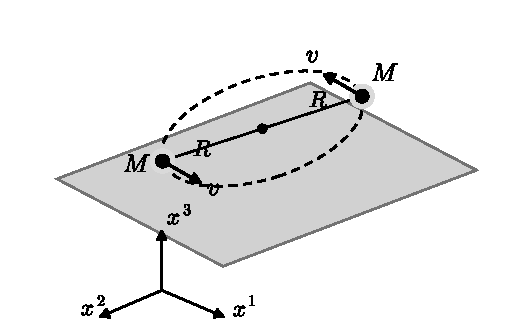
\includegraphics[width=0.72\textwidth]{fig_7.10.pdf}
\caption*{图 7.10\quad 一个双星系统。两颗质量为 $M$ 的恒星在 $x^1$-$x^2$ 平面内以轨道半径 $R$ 绕转。}
\end{figure}

用 $\Omega$ 我们可以写出恒星 $a$ 的显式轨迹，
\begin{equation*}
x^{1}_{a} = R\cos\Omega t, \qquad x^{2}_{a} = R\sin\Omega t,
\tag{7.145}
\end{equation*}
以及恒星 $b$ 的轨迹，
\begin{equation*}
x^{1}_{b} = -R\cos\Omega t, \qquad x^{2}_{b} = -R\sin\Omega t.
\tag{7.146}
\end{equation*}
相应的能量密度为
\begin{equation*}
T^{00}(t, \mathbf{x}) = M\delta(x^{3})\left[\delta(x^{1} - R\cos\Omega t)\delta(x^{2} - R\sin\Omega t) + \delta(x^{1} + R\cos\Omega t)\delta(x^{2} + R\sin\Omega t)\right].
\tag{7.147}
\end{equation*}
这些密密麻麻的 $\delta$ 函数使我们能够直接积分，由 (7.138) 得到四极矩：
\begin{align*}
I_{11} &= 2MR^{2}\cos^{2}\Omega t = MR^{2}(1 + \cos 2\Omega t) \\
I_{22} &= 2MR^{2}\sin^{2}\Omega t = MR^{2}(1 - \cos 2\Omega t) \\
I_{12} &= I_{21} = 2MR^{2}(\cos\Omega t)(\sin\Omega t) = MR^{2}\sin 2\Omega t \\
I_{i3} &= 0.
\tag{7.148}
\end{align*}
由此再利用 (7.140)，容易得到度规微扰的分量：

% ---- 书页 307 / p322 ----

\begin{equation*}
\bar{h}_{ij}(t, \mathbf{x}) = \frac{8GM}{r}\Omega^{2}R^{2}
\begin{pmatrix}
-\cos 2\Omega t_r & -\sin 2\Omega t_r & 0 \\
-\sin 2\Omega t_r & \cos 2\Omega t_r & 0 \\
0 & 0 & 0
\end{pmatrix}.
\tag{7.149}
\end{equation*}
$\bar{h}_{\mu\nu}$ 的其余分量可以通过要求 Lorenz 规范条件得到满足而导出。

\section{引力辐射导致的能量损失}

到了这里，很自然想谈谈通过引力辐射发射的能量。然而这样的讨论立刻就会遇到种种问题，既有技术上的，也有哲学上的。正如我们前面提到过的，引力场中的能量没有真正的局域量度。当然，在弱场极限下——即我们把引力当作是在固定背景度规上传播的对称张量来描述——我们或许有望像对电磁学或其他任何场论那样，导出涨落 $h_{\mu\nu}$ 的能量-动量张量。在某种程度上这是可能的，但仍然困难。由于这些困难，文献中有许多不同的建议，关于在弱场极限下应当用什么作为引力的能量-动量张量；它们彼此不同，但对于诸如双星系统能量发射速率这类物理上适定的问题，它们给出的答案大体相同。

在技术层面上，当我们考虑能量-动量张量应当取什么形式时，困难开始出现。我们前面提到过电磁学和标量场论的能量-动量张量，两者共有一个重要特征——它们都是相关场的二次式。按照假设，我们处理弱场极限的办法是只保留度规微扰的线性项。因此，为了追踪引力波携带的能量，我们将不得不把计算扩展到至少 $h_{\mu\nu}$ 的二阶。事实上，我们一直都在稍稍作弊。在讨论引力波对检验粒子的效应以及双星系统产生波时，我们一直在利用检验粒子沿测地线运动这一事实。但我们知道，这是从能量-动量的协变守恒 $\nabla_\mu T^{\mu\nu} = 0$ 推出来的；然而在我们一直工作的阶次上，实际有的是 $\partial_\mu T^{\mu\nu} = 0$，而那将意味着检验粒子在平直背景度规中沿直线运动。这是弱场极限无法描述自引力系统的一个症状。在实践中，最好的办法是把弱场方程解到某个适当的阶，然后再事后论证解的有效性。我们将遵循 Misner, Thorne 和 Wheeler (1973) 第 35、36 章概述的程序，那里可以找到关于这些微妙之处的更多讨论。另见 Wald (1984) 与 Schutz (1985)。

现在让我们考察 Einstein 真空方程 $R_{\mu\nu} = 0$ 到二阶，看看结果如何能用引力场的能量-动量张量来解释。我们把度规和 Ricci 张量都展开，

% ---- 书页 308 / p323 ----

\begin{gather*}
g_{\mu\nu} = \eta_{\mu\nu} + h^{(1)}_{\mu\nu} + h^{(2)}_{\mu\nu} \\
R_{\mu\nu} = R^{(0)}_{\mu\nu} + R^{(1)}_{\mu\nu} + R^{(2)}_{\mu\nu},
\tag{7.150}
\end{gather*}
其中 $R^{(1)}_{\mu\nu}$ 取为与 $h^{(1)}_{\mu\nu}$ 同阶，而 $R^{(2)}_{\mu\nu}$ 与 $h^{(2)}_{\mu\nu}$ 则是 $(h^{(1)}_{\mu\nu})^{2}$ 阶的。因为我们在平直背景中工作，零阶方程 $R^{(0)}_{\mu\nu} = 0$ 自动满足。一阶真空方程就是
\begin{equation*}
R^{(1)}_{\mu\nu}[h^{(1)}] = 0,
\tag{7.151}
\end{equation*}
它确定一阶微扰 $h^{(1)}_{\mu\nu}$（相差规范变换）。二阶微扰 $h^{(2)}_{\mu\nu}$ 则将由二阶方程
\begin{equation*}
R^{(1)}_{\mu\nu}[h^{(2)}] + R^{(2)}_{\mu\nu}[h^{(1)}] = 0.
\tag{7.152}
\end{equation*}
确定。记号 $R^{(1)}_{\mu\nu}[h^{(2)}]$ 表示展开后的 Ricci 张量中与度规微扰呈线性关系的那些部分，也就是把由 (7.6) 给出的表达式应用于二阶微扰 $h^{(2)}_{\mu\nu}$；与此同时，$R^{(2)}_{\mu\nu}[h^{(1)}]$ 代表展开后 Ricci 张量的二次部分，
\begin{align*}
R^{(2)}_{\mu\nu} ={}& \frac{1}{2}h^{\rho\sigma}\partial_\mu\partial_\nu h_{\rho\sigma} + \frac{1}{4}(\partial_\mu h_{\rho\sigma})\partial_\nu h^{\rho\sigma} + (\partial^\sigma h^{\rho}{}_{\nu})\partial_{[\sigma}h_{\rho]\mu} - h^{\rho\sigma}\partial_\rho\partial_{(\mu}h_{\nu)\sigma} \\
&+ \frac{1}{2}\partial_\sigma(h^{\rho\sigma}\partial_\rho h_{\mu\nu}) - \frac{1}{4}(\partial_\rho h_{\mu\nu})\partial^\rho h - \left(\partial_\sigma h^{\rho\sigma} - \frac{1}{2}\partial^\sigma h\right)\partial_{(\mu}h_{\nu)\rho},
\tag{7.153}
\end{align*}
把它应用于一阶微扰 $h^{(1)}_{\mu\nu}$。没有交叉项，因为它们必然是更高阶的。

现在让我们把真空方程写成 $G_{\mu\nu} = 0$；这当然等价于 $R_{\mu\nu} = 0$，但能使我们以富有启发性的形式表达结果。在二阶我们有
\begin{equation*}
R^{(1)}_{\mu\nu}[h^{(2)}] - \frac{1}{2}\eta^{\rho\sigma}R^{(2)}_{\rho\sigma}[h^{(2)}]\eta_{\mu\nu} = 8\pi G t_{\mu\nu},
\tag{7.154}
\end{equation*}
其中我们定义了
\begin{equation*}
t_{\mu\nu} \equiv -\frac{1}{8\pi G}\left\{R^{(2)}_{\mu\nu}[h^{(1)}] - \frac{1}{2}\eta^{\rho\sigma}R^{(2)}_{\rho\sigma}[h^{(1)}]\eta_{\mu\nu}\right\}.
\tag{7.155}
\end{equation*}
关于这个表达式注意两点。第一，我们没有包含形如 $h^{(1)\rho\sigma}R^{(1)}_{\rho\sigma}[h^{(1)}]$ 的项，因为 $R^{(1)}_{\mu\nu}[h^{(1)}] = 0$。第二，(7.154) 的左边并不是完整的二阶 Einstein 张量，因为我们把涉及 $R^{(2)}_{\mu\nu}[h^{(1)}]$ 的项移到了右边，并大胆地把它们重新标记为一阶微扰的能量-动量张量 $t_{\mu\nu}$。这样一种认定看来非常有理：

% ---- 书页 309 / p324 ----（承接上页末"……这样一种认定看来非常有理："）

$t_{\mu\nu}$ 是一个对称张量，是 $h_{\mu\nu}$ 的二次式，它恰好以物质能量-动量张量会采取的方式表示微扰如何影响时空度规。（$h_{\mu\nu}$ 的线性项不起作用，因为 $G^{(1)}_{\mu\nu}[h^{(1)}]$ 已被一阶方程直接置为零。）注意，$t_{\mu\nu}$ 也是守恒的，在背景平直空间的意义下，
\begin{equation*}
\partial_\mu t^{\mu\nu} = 0,
\tag{7.156}
\end{equation*}
这从 Bianchi 恒等式 $\partial_\mu G^{\mu\nu} = 0$ 就可以知道。

遗憾的是，把 $t_{\mu\nu}$ 解释为能量-动量张量存在一些局限。当然，在完整的理论中它根本不是张量，但根据假设我们对这一点不予理会。更重要的是，它在规范变换（无穷小微分同胚）下不是不变的，你可以通过直接计算来验证这一点。绕开这个困难的一种办法，是把能量-动量张量在若干个波长上取平均，我们用尖括号 $\langle\cdots\rangle$ 表示这一操作。这一做法兼有哲学上和实用上的优点。从哲学的观点看，我们知道，正因为可以在任意一点选取 Riemann 法坐标，我们不可能定义一种纯粹局域的（在每一点恰好用该点的度规及其一阶导数来定义的）、可靠的引力能量-动量量度。然而，如果在若干个波长上取平均，我们就有希望捕捉到一个小区域内足够多的物理曲率，从而给出一个规范不变的量度。从实用的角度看，任何导数项（相对于导数的乘积）平均后都为零，
\begin{equation*}
\langle\partial_\mu(X)\rangle = 0.
\tag{7.157}
\end{equation*}
因此我们就有理由在平均括号下分部积分，
\begin{equation*}
\langle A(\partial_\mu B)\rangle = -\langle(\partial_\mu A)B\rangle,
\tag{7.158}
\end{equation*}
这将大大简化我们的表达式。

考虑到这些，让我们用二阶 Ricci 张量的表达式 (7.153) 来计算 (7.155) 定义的 $t_{\mu\nu}$。（从此以后我们将不再在度规微扰上写上标，因为我们只对一阶微扰感兴趣。）虽然取平均的部分动机是得到规范不变的答案，但实际计算相当繁难，所以为了演示，我们将在横无迹规范下进行，
\begin{equation*}
\partial^{\mu}h^{\mathrm{TT}}_{\mu\nu} = 0, \qquad h^{\mathrm{TT}} = 0.
\tag{7.159}
\end{equation*}
不要忘了，只有在真空中我们才被允许选取这个规范。在这个规范下，$R^{(2)\mathrm{TT}}_{\mu\nu}$ 的非零部分可以写成
\begin{align*}
R^{(2)\mathrm{TT}}_{\mu\nu} ={}& \frac{1}{2}h^{\rho\sigma}_{\mathrm{TT}}\partial_\mu\partial_\nu h^{\mathrm{TT}}_{\rho\sigma} + \frac{1}{4}(\partial_\mu h^{\mathrm{TT}}_{\rho\sigma})\partial_\nu h^{\rho\sigma}_{\mathrm{TT}} + \frac{1}{2}\eta^{\rho\lambda}(\partial^\sigma h^{\mathrm{TT}}_{\rho\nu})\partial_\sigma h^{\mathrm{TT}}_{\lambda\mu} \\
&- \frac{1}{2}(\partial^\sigma h^{\mathrm{TT}}_{\rho\nu})\partial^\rho h^{\mathrm{TT}}_{\sigma\mu} - h^{\rho\sigma}_{\mathrm{TT}}\partial_\sigma\partial_{(\mu}h^{\mathrm{TT}}_{\nu)\rho} + \frac{1}{2}h^{\rho\sigma}_{\mathrm{TT}}\partial_\sigma\partial_\rho h^{\mathrm{TT}}_{\mu\nu}.
\tag{7.160}
\end{align*}

% ---- 书页 310 / p325 ----

现在让我们施加平均括号，并在方便之处分部积分。(7.160) 的最后三项全部消失，因为分部积分给出的散度最终化为零。于是剩下
\begin{equation*}
\left\langle R^{(2)\mathrm{TT}}_{\mu\nu}\right\rangle = -\frac{1}{4}\left\langle(\partial_\mu h^{\mathrm{TT}}_{\rho\sigma})(\partial_\nu h^{\rho\sigma}_{\mathrm{TT}}) + 2\eta^{\rho\lambda}(\Box h^{\mathrm{TT}}_{\rho\nu})h^{\mathrm{TT}}_{\lambda\mu}\right\rangle.
\tag{7.161}
\end{equation*}
但微扰服从一阶运动方程，它令 $\Box h^{\mathrm{TT}}_{\mu\nu} = 0$。所以我们最终剩下
\begin{equation*}
\left\langle R^{(2)\mathrm{TT}}_{\mu\nu}\right\rangle = -\frac{1}{4}\left\langle(\partial_\mu h^{\mathrm{TT}}_{\rho\sigma})(\partial_\nu h^{\rho\sigma}_{\mathrm{TT}})\right\rangle.
\tag{7.162}
\end{equation*}
我们可以取迹得到标量曲率；分部积分之后我们再次遇到一个 $\Box h^{\mathrm{TT}}_{\mu\nu}$ 项，我们把它置为零，于是
\begin{equation*}
\left\langle\eta^{\mu\nu}R^{(2)\mathrm{TT}}_{\mu\nu}\right\rangle = 0.
\tag{7.163}
\end{equation*}
把这些表达式代入 (7.155)，就得到横无迹规范下引力波能量-动量张量的一个简单表达式：
\begin{equation*}
\boxed{\,t_{\mu\nu} = \frac{1}{32\pi G}\left\langle(\partial_\mu h^{\mathrm{TT}}_{\rho\sigma})(\partial_\nu h^{\rho\sigma}_{\mathrm{TT}})\right\rangle.\,}
\tag{7.164}
\end{equation*}
记住，在这个规范下非空间分量为零，$h^{\mathrm{TT}}_{0\nu} = 0$。因此你有时会看到上面的表达式用空间指标 $ij$ 而不是时空指标 $\rho\sigma$ 来写；两种写法显然等价。如果我们足够强大，能够不先选定规范就完成相应的计算，我们将会发现
\begin{align*}
t_{\mu\nu} = \frac{1}{32\pi G}\Big\langle(\partial_\mu h_{\rho\sigma})(\partial_\nu h^{\rho\sigma}) &- \frac{1}{2}(\partial_\mu h)(\partial_\nu h) \\
&- (\partial_\rho h^{\rho\sigma})(\partial_\mu h_{\nu\sigma}) - (\partial_\rho h^{\rho\sigma})(\partial_\nu h_{\mu\sigma})\Big\rangle.
\tag{7.165}
\end{align*}
稍作直接的处理便足以验证这个表达式其实是规范不变的，习题中会请你证明这一点。

让我们对单个平面波计算横无迹表达式 (7.164)，
\begin{equation*}
h^{\mathrm{TT}}_{\mu\nu} = C_{\mu\nu}\sin(k_\lambda x^\lambda).
\tag{7.166}
\end{equation*}
我们取了实部，并任意设定相位，使这个波是正弦而非余弦。于是能量-动量张量为
\begin{equation*}
t_{\mu\nu} = \frac{1}{32\pi G}k_\mu k_\nu C_{\rho\sigma}C^{\rho\sigma}\left\langle\cos^{2}(k_\lambda x^\lambda)\right\rangle.
\tag{7.167}
\end{equation*}

% 本块末段在原书书页 310 末 (7.167) 处截断，其后文字于书页 311 顶部继续；下一块应续接本段。

% ==== tail：7.6 节收尾（承接书页 310，从 (7.168) 起），置于下一个 \section 之前 ====

% ---- 书页 311 / p326 ----

把 $\cos^2$ 项在几个波长上取平均，得到
\begin{equation*}
\left\langle \cos^2(k_\lambda x^\lambda) \right\rangle = \frac{1}{2}.
\tag{7.168}
\end{equation*}
为简单起见，我们可以取波沿 $z$ 轴传播，于是
\begin{equation*}
k_\lambda = \left(-\omega,\, 0,\, 0,\, \omega\right)
\tag{7.169}
\end{equation*}
负号来自把 $k^\lambda$ 的一个指标降下来；再利用 (7.109)，得到
\begin{equation*}
C_{\rho\sigma}C^{\rho\sigma} = 2(h_+^2 + h_\times^2).
\tag{7.170}
\end{equation*}
在引力波文献中，更常见的做法是用普通频率 $f = \omega/2\pi$ 而不是角频率 $\omega$ 来表达可观测量。把上面的结果合在一起，就得到
\begin{equation*}
t_{\mu\nu} = \frac{\pi}{8G}f^2(h_+^2 + h_\times^2)
\begin{pmatrix}
1 & 0 & 0 & -1 \\
0 & 0 & 0 & 0 \\
0 & 0 & 0 & 0 \\
-1 & 0 & 0 & 1
\end{pmatrix}.
\tag{7.171}
\end{equation*}
正如我们在下一节将要讨论的，我们有望在地球上观测到的典型引力波源，频率介于 $10^{-4}$ 与 $10^4\,\mathrm{Hz}$ 之间，振幅 $h \sim 10^{-22}$。因此，把沿 $z$ 方向的能量流 $-T_{0z}$ 用数量级的形式表示出来是有用的：
\begin{equation*}
-T_{0z} \sim 10^{-4}\left(\frac{f}{\mathrm{Hz}}\right)^{2}\frac{\left(h_+^2 + h_\times^2\right)}{\left(10^{-21}\right)^{2}}\ \frac{\mathrm{erg}}{\mathrm{cm}^2\cdot\mathrm{s}}.
\tag{7.172}
\end{equation*}
这就是原则上每秒钟可以沉积到探测器每平方厘米中的能量。正如 Thorne\footnote{K.S.~Thorne, 载于 \emph{Three Hundred Years of Gravitation}, Cambridge: Cambridge University Press, 1987。}所指出的，这实际上是相当可观的能量流，尤其是在频率范围的高端。作为比较，处于宇宙学距离上的超新星，其峰值电磁流量约为 $10^{-9}\,\mathrm{erg/cm^2/s}$；然而引力波信号只持续几毫秒，而可见的电磁信号却能延续数月。

现在让我们用引力波能量-动量张量的公式，来计算一个按四极公式 (7.140) 发出引力辐射的系统的能量损失率。在一个常值时间的曲面 $\Sigma$ 上所包含的引力辐射总能量定义为
\begin{equation*}
E = \int_{\Sigma} t_{00}\, d^3x,
\tag{7.173}
\end{equation*}
而辐射到无穷远处的总能量则可以表示为

% ---- 书页 312 / p327 ----

\begin{equation*}
\Delta E = \int P\, dt,
\tag{7.174}
\end{equation*}
其中功率 $P$ 为
\begin{equation*}
P = \int_{S^2_\infty} t_{0\mu}n^\mu r^2\, d\Omega.
\tag{7.175}
\end{equation*}
这里，积分取在空间无穷远处的二维球面 $S^2_\infty$ 上，而 $n^\mu$ 是垂直于 $S^2_\infty$ 的单位类空矢量。在极坐标 $\{t, r, \theta, \phi\}$ 中，法矢量的分量为
\begin{equation*}
n^\mu = (0,\, 1,\, 0,\, 0).
\tag{7.176}
\end{equation*}

我们想用 $t_{\mu\nu}$ 的表达式 (7.164) 来计算功率 $P$。面临的第一个问题是，这个表达式是用横无迹微扰写下的，而四极公式 (7.140) 却是用 Lorenz 规范下无迹反转微扰的空间分量 $h_{ij}$ 写下的。最简单的步骤（虽然它也没那么简单）是先把 $h_{ij}$ 转换到横无迹规范——由于我们关心的是波在远离其发射源的真空中的行为，这样做是允许的——代入 $t_{\mu\nu}$ 的公式，然后再转换回非横无迹的形式。让我们看看这一套流程是如何进行的。

我们首先引入（空间的）投影张量
\begin{equation*}
P_{ij} = \delta_{ij} - n_i n_j,
\tag{7.177}
\end{equation*}
它把张量分量投影到与单位矢量 $n^i$ 正交的曲面上。（更详细的讨论见附录 D。）在我们的情形中，我们取 $n^i$ 沿波的传播方向，这样 $P_{ij}$ 便投影到空间无穷远处的二维球面上。我们可以用这个投影张量，按下式构造对称空间张量 $X_{ij}$ 的横无迹版本：
\begin{equation*}
X^{\mathrm{TT}}_{ij} = \left(P_i{}^k P_j{}^l - \frac{1}{2}P_{ij}P^{kl}\right)X_{kl}.
\tag{7.178}
\end{equation*}
你可以自行验证 $X^{\mathrm{TT}}_{ij}$ 确实是横向且无迹的。由于它无迹，$\bar{h}^{\mathrm{TT}}_{ij}$ 就等于原来的微扰 $h^{\mathrm{TT}}_{ij}$；代入四极公式 (7.140)，我们得到
\begin{equation*}
h^{\mathrm{TT}}_{ij} = \bar{h}^{\mathrm{TT}}_{ij} = \frac{2G}{r}\frac{d^2 I^{\mathrm{TT}}_{ij}}{dt^2}(t - r),
\tag{7.179}
\end{equation*}
其中四极矩的横无迹部分同样按 (7.178) 构造。事实上，由 (7.138) 定义的四极矩并不是用来表达所生成的波的最方便的量，因为它涉及一个
% ---- 书页 313 / p328 ----
对能量密度的积分，而这个积分可能难以确定。我们可以改用\textbf{约化四极矩}（reduced quadrupole moment）
\begin{equation*}
J_{ij} = I_{ij} - \frac{1}{3}\delta_{ij}\delta^{kl}I_{kl},
\tag{7.180}
\end{equation*}
它正是 $I_{ij}$ 的无迹部分。约化四极矩有一个很好的性质：它是 Newton 势多极展开中 $r^{-3}$ 项的系数，
\begin{equation*}
\Phi = -\frac{GM}{r} - \frac{G}{r^3}D_i x^i - \frac{3G}{2r^5}J_{ij}x^i x^j + \cdots,
\tag{7.181}
\end{equation*}
因此对于现实的源更容易近似。（这里 $D_i$ 是偶极矩，$D_i = \int T^{00}x^i\, d^3x$。）当然，四极矩的横无迹部分与约化（也就是无迹）四极矩的横无迹部分是一样的，所以 (7.179) 变为
\begin{equation*}
h^{\mathrm{TT}}_{ij} = \frac{2G}{r}\frac{d^2 J^{\mathrm{TT}}_{ij}}{dt^2}(t - r).
\tag{7.182}
\end{equation*}

为了计算功率，我们关心的是 $t_{0\mu}n^\mu = t_{0r}$。由于四极矩只依赖于推迟时间（retarded time）$t_r = t - r$，我们有
\begin{align*}
\partial_0 h^{\mathrm{TT}}_{ij} &= \frac{2G}{r}\frac{d^3 J^{\mathrm{TT}}_{ij}}{dt^3},\\
\partial_r h^{\mathrm{TT}}_{ij} &= -\frac{2G}{r}\frac{d^3 J^{\mathrm{TT}}_{ij}}{dt^3} - \frac{2G}{r^2}\frac{d^2 J^{\mathrm{TT}}_{ij}}{dt^2}\\
&\approx -\frac{2G}{r}\frac{d^3 J^{\mathrm{TT}}_{ij}}{dt^3},
\tag{7.183}
\end{align*}
其中我们已经去掉了 $r^{-2}$ 项，因为我们关心的是 $r \to \infty$ 的极限。于是，能量-动量张量的重要分量为
\begin{equation*}
t_{0r} = -\frac{G}{8\pi r^2}\left\langle\left(\frac{d^3 J^{\mathrm{TT}}_{ij}}{dt^3}\right)\left(\frac{d^3 J_{\mathrm{TT}}^{ij}}{dt^3}\right)\right\rangle.
\tag{7.184}
\end{equation*}
下一步是从横无迹部分转换回 $J_{ij}$。应用 (7.178) 以及一些繁琐的代数运算，可以直接证明
\begin{equation*}
X^{\mathrm{TT}}_{ij}X_{\mathrm{TT}}^{ij} = X_{ij}X^{ij} - 2X_i{}^j X^{ik}n_j n_k + \frac{1}{2}X^{ij}X^{kl}n_i n_j n_k n_l - \frac{1}{2}X^2 + XX^{ij}n_i n_j,
\tag{7.185}
\end{equation*}
其中 $X = \delta^{ij}X_{ij}$。由于 $J_{ij}$ 是无迹的，我们有
\begin{equation*}
J^{\mathrm{TT}}_{ij}J_{\mathrm{TT}}^{ij} = J_{ij}J^{ij} - 2J_i{}^j J^{ik}n_j n_k + \frac{1}{2}J^{ij}J^{kl}n_i n_j n_k n_l,
\tag{7.186}
\end{equation*}

% ---- 书页 314 / p329 ----

而功率为
\begin{align*}
P = -\frac{G}{8\pi}\int_{S^2_\infty}\bigg\langle \frac{d^3 J_{ij}}{dt^3}\frac{d^3 J^{ij}}{dt^3} &- 2\frac{d^3 J_i{}^j}{dt^3}\frac{d^3 J^{ik}}{dt^3}n_j n_k\\
&+ \frac{1}{2}\frac{d^3 J^{ij}}{dt^3}\frac{d^3 J^{kl}}{dt^3}n_i n_j n_k n_l\bigg\rangle\, d\Omega.
\tag{7.187}
\end{align*}
要求出这个表达式的值，最好换回到空间的笛卡尔坐标，其中 $n^i = x^i/r$。四极张量与角坐标无关，因为它们是由对全空间的积分定义的。于是我们可以把它们移到积分号外，并利用恒等式
\begin{align*}
\int d\Omega &= 4\pi\\
\int n_i n_j\, d\Omega &= \frac{4\pi}{3}\delta_{ij}\\
\int n_i n_j n_k n_l\, d\Omega &= \frac{4\pi}{15}\left(\delta_{ij}\delta_{kl} + \delta_{ik}\delta_{jl} + \delta_{il}\delta_{jk}\right).
\tag{7.188}
\end{align*}
当一切尘埃落定，功率的表达式便塌缩为
\begin{equation*}
P = -\frac{G}{5}\left\langle \frac{d^3 J_{ij}}{dt^3}\frac{d^3 J^{ij}}{dt^3}\right\rangle,
\tag{7.189}
\end{equation*}
这里我们应当记住，四极矩是在推迟时间 $t_r = t - r$ 处取值的。我们的公式带有一个负号，因为它表示的是能量变化的速率，而辐射源将不断损失能量。

对于由 (7.148) 所表示的双星系统，约化四极矩为
\begin{equation*}
J_{ij} = \frac{MR^2}{3}
\begin{pmatrix}
(1+3\cos 2\Omega t) & 3\sin 2\Omega t & 0\\
3\sin 2\Omega t & (1-3\cos 2\Omega t) & 0\\
0 & 0 & -2
\end{pmatrix},
\tag{7.190}
\end{equation*}
它对时间的三阶导数于是为
\begin{equation*}
\frac{d^3 J_{ij}}{dt^3} = 8MR^2\Omega^3
\begin{pmatrix}
\sin 2\Omega t & -\cos 2\Omega t & 0\\
-\cos 2\Omega t & -\sin 2\Omega t & 0\\
0 & 0 & 0
\end{pmatrix}.
\tag{7.191}
\end{equation*}
于是双星辐射的功率为
\begin{equation*}
P = -\frac{128}{5}GM^2R^4\Omega^6,
\tag{7.192}
\end{equation*}
或者，利用 (7.144) 的频率表达式，
\begin{equation*}
P = -\frac{2}{5}\frac{G^4M^5}{R^5}.
\tag{7.193}
\end{equation*}

% ---- 书页 315 / p330 ----

当然，通过发射引力辐射而损失能量的现象已经被观测到了。1974 年，Hulse 和 Taylor 发现了一个双星系统 PSR~1913+16，其中的两颗星都非常小，因此经典效应可以忽略，或者至少是可控的，而且其中一颗是脉冲星。轨道周期为八小时，按天体物理的标准衡量极其短。其中一颗星是脉冲星这个事实提供了一个非常精确的时钟，借助它便可以测量系统损失能量时周期的变化。这个结果与广义相对论关于引力辐射导致能量损失的预言相一致。

\section{引力波的探测}

当代引力物理和天体物理学最优先的目标之一，是直接探测引力辐射。（所谓“直接”，我们的意思是“通过观测引力波对检验物体的影响”，与之相对的是观测能量损失的间接效应，就像脉冲双星中的情形。）完全有理由相信，这样的探测很快就会实现，或者是在已经建成的引力波天文台中，或者是在近期正在规划的引力波天文台中。当然，一旦我们探测到了引力辐射，目标就会立刻变成从观测中提取有用的天体物理信息。我们目前对太阳系之外宇宙的认识，几乎完全来自对电磁辐射的观测，外加一些来自中微子和宇宙线的输入；引力波天体物理学的到来，将打开一扇通往遥远宇宙中高能现象的全新窗口。\footnote{关于引力波天体物理学的概览，见 S.A.~Hughes, S.~Márka, P.L.~Bender 与 C.J.~Hogan, “New physics and astronomy with the new gravitational-wave observatories,” \texttt{http://arxiv.org/astro-ph/0110349}。}

在讨论我们可以如何着手探测天体物理引力波之前，我们应该想一想哪些源最容易被观测到。第一个重要的认识是：产生可观引力辐射所需的条件，与产生电磁辐射所需的条件非常不同。这个差别可以追溯到这样一个事实：引力波由大质量物体的整体运动（bulk motion）产生，而电磁波（通常）由单个粒子的不相干激发产生。因此，电磁辐射可以由一个整体上静态的源产生，比如一颗恒星，这对天文学家来说是一大优势。然而，引力波是由大块运动着的物质相干地产生的（物质中的每个粒子都以相同的方式对波有所贡献），这可以部分弥补静态源无法发射引力波的缺憾。

因此，我们需要具有可观整体运动的大质量源。作为一个简单的例子，考虑 7.5 节中的双星系统，其中两颗星的质量都是 $M$，轨道半径为 $R$。我们将稍微作一点弊，把 Newton 的轨道参数公式用到广义相对论已经开始变得重要的区域，不过对于数量级的估计这已经足够了。相关参数可以归结为 Schwarzschild 半径 $R_S = 2GM/c^2$、
% ---- 书页 316 / p331 ----
轨道半径 $R$，以及我们与双星之间的距离 $r$。（现在我们将把因子 $c$ 显式地恢复，以便与实验比较。）用这些量来表示，轨道的频率——也即所产生的引力波的频率——近似为
\begin{equation*}
f = \frac{\Omega}{2\pi} \sim \frac{cR_S^{1/2}}{10R^{3/2}}.
\tag{7.194}
\end{equation*}
利用 (7.149) 中关于所产生的微扰的公式，我们可以估计接收到的引力波振幅为
\begin{equation*}
h \sim \frac{R_S^2}{rR}.
\tag{7.195}
\end{equation*}
让我们看看，这对我们有望观测到的那一类源意味着什么。一个范例性的例子是黑洞/黑洞双星的并合（coalescence）。对于典型的参数，我们可以取两个黑洞都是 10 倍太阳质量，双星处于约 100 Mpc 的宇宙学距离上，而两颗子星相距为其 Schwarzschild 半径的十倍：
\begin{gather*}
R_S \sim 10^6\,\mathrm{cm}\\
R \sim 10^7\,\mathrm{cm}\\
r \sim 10^{26}\,\mathrm{cm}.
\tag{7.196}
\end{gather*}
这样的源因而具有如下特征量级：
\begin{equation*}
f \sim 10^2\,\mathrm{s}^{-1}, \qquad h \sim 10^{-21}.
\tag{7.197}
\end{equation*}
如果我们还想有希望探测到具有这些参数的双星并合，我们就需要对 100 Hz 附近的频率以及 $10^{-21}$ 或更小量级的应变足够敏感。

所幸的是，这些参数处于我们实验能力（在许多科学家英勇的努力之下）所能及的范围之内。目前正在考虑的引力波探测方案中最有前途的技术是干涉测量法，因此这里我们将只讨论干涉仪，尽管完全可以设想，将来会发明出具有更好灵敏度的新技术。

回想一下，引力波经过时的物理效应是轻微地扰动自由下落的质量之间的相对位置。如果两个检验质量（test masses）相距 $L$，它们之间距离的变化大致为
\begin{equation*}
\frac{\delta L}{L} \sim h.
\tag{7.198}
\end{equation*}
设想我们打算建造一座检验物体相距公里量级的天文台。那么，要探测振幅为
% ---- 书页 317 / p332 ----
$h\sim 10^{-21}$ 量级的波，就需要对量级为
\begin{equation*}
\delta L \sim 10^{-16}\left(\frac{h}{10^{-21}}\right)\left(\frac{L}{\mathrm{km}}\right)\,\mathrm{cm}
\tag{7.199}
\end{equation*}
的变化具有足够的灵敏度。把它与一个典型原子的大小比较一下——后者由玻尔半径（Bohr radius）给出，
\begin{equation*}
a_0 \sim 5\times 10^{-9}\,\mathrm{cm},
\tag{7.200}
\end{equation*}
或者，也不妨与一个典型原子核的大小比较——大约一个费米（Fermi），
\begin{equation*}
1\,\mathrm{fm} = 10^{-13}\,\mathrm{cm}.
\tag{7.201}
\end{equation*}
我们在这里反复强调的要点是：一座切实可行的地面引力波天文台，必须对距离变化足够敏感——要比任何可以设想的检验质量所必须由之构成的那些原子的大小还要小得多。

\begin{figure}[H]
\centering
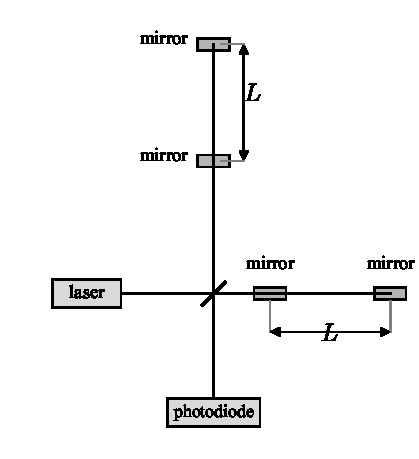
\includegraphics[width=0.72\textwidth]{fig_7.11.pdf}
\caption*{图 7.11\quad 引力波干涉仪的示意图。}
\end{figure}

激光干涉仪提供了一条克服测量如此微小扰动之困难的途径。考虑图 7.11 所描绘的示意图装置。一束激光（典型特征波长 $\lambda \sim 10^{-4}\,\mathrm{cm}$）被导向一个分束器（beamsplitter），分束器把光子送进两条抽成真空的、长度为 $L$ 的管道。腔的末端是检验质量，用悬挂在摆上的反射镜来表示。光实际上是在分束器附近的部分反射镜（partially-reflective mirrors）之间来回反射的，所以一个典型的光子在回到分束器并被导入
% ---- 书页 318 / p333 ----
光电二极管之前，会在腔内上下往返约 100 次。整个系统的安排是这样的：如果检验质量完全静止，返回的两束光将发生相消干涉，光电二极管接收不到任何信号。正如我们已经看到的，引力波经过的效应是把相互正交的长度朝相反的方向扰动，这会引起激光脉冲的相移，从而破坏相消干涉。在腔臂中往返 100 次的过程中，累积的相移将为
\begin{equation*}
\delta\phi \sim 200\left(\frac{2\pi}{\lambda}\right)\delta L \sim 10^{-9},
\tag{7.202}
\end{equation*}
其中用 200 而不是 100，反映的是两臂中的相移会相加这一事实。这样微小的相移是可以测量的，只要光子数 $N$ 足够大，足以克服“散粒噪声”（shot noise）；具体地说，只要 $\sqrt{N} > \delta\phi$。

建造足够“安静”且灵敏的引力波天文台所面临的技术挑战，正在多个不同的地方被攻克，包括美国（LIGO）、意大利（Virgo）、德国（GEO）、日本（TAMA）和澳大利亚（ACIGA）。LIGO（激光干涉引力波天文台，Laser Interferometric Gravitational-Wave Observatory）是目前最先进的探测器；它由两个设施组成（一个在华盛顿州，一个在路易斯安那州），每个都有四公里长的臂。单一的引力波天文台将无法对源在天空中的位置定位；要完成这一任务，多个探测器至关重要（这对于验证一个表观信号是否真实同样关键）。

基本的噪声来源限制了地面天文台探测低频引力波的能力。图 7.12 展示了两种截然不同的设计——LIGO 这样的地面天文台，以及 LISA（激光干涉空间天线，Laser Interferometer Space Antenna）这样的空间任务——的灵敏度区域随频率的变化。LISA 背后的一般原理与其他任何干涉仪相同，但其实施方案则（如果它真的被建造的话，或者说将会）截然不同。目前的设计设想三个航天器绕太阳运行，位于地球后方约三千万公里处，彼此相距五百万公里。由于间隔大得多，LISA 对 $10^{-2}\,\mathrm{Hz}$ 附近的频率敏感。这张图中所描绘的灵敏度只能视为示意性的，因为它们依赖于积分时间和其他因素。

许多潜在的噪声源摆在了引力波天文学家的面前。对于地面天文台，低频处占主导的效应通常是地震噪声（seismic noise），高频处的效应来自光子散粒噪声，中间频率处则来自热噪声。地面探测器的改进版本也许能够补偿低频的地震噪声，但会遇到来自大气现象或附近经过的物体（比如汽车）的引力梯度所带来的不可约噪声。卫星天文台当然对这类效应免疫。相反，其根本限制预期来自测量航天器之间距离变化时的误差（更确切地说，是航天器内部受到屏蔽的检验质量之间的距离变化），以及航天器的非引力加速度。

% ---- 书页 319 / p334 ----

\begin{figure}[H]
\centering
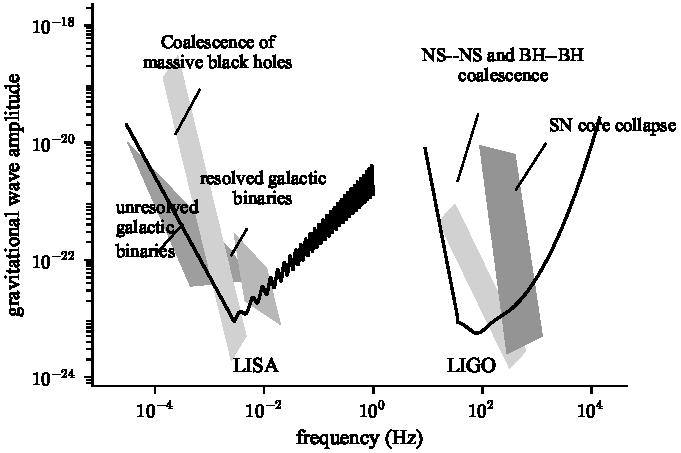
\includegraphics[width=0.72\textwidth]{fig_7.12.pdf}
\caption*{图 7.12\quad 代表性的地面（LIGO）与空间（LISA）引力波天文台的灵敏度随频率的变化，以及各种可能的源所预期的信号。图取自 LISA 合作组主页（\texttt{http://lisa.jpl.nasa.gov/}）。}
\end{figure}

最后，我们可以对引力波天文台各种可能的源作一个十分简要的概述。我们已经提到过各种类型的致密双星。对于地面天文台，这类源要等到非常接近并合时才会变得可见，而且前提是两颗子星的质量足够大（中子星或黑洞）。根据我们对这类系统的认识作外推，在几百 Mpc 的距离之内每年也许会有几次并合。另一个有希望的可能性是大质量恒星的核心坍缩（core collapse），即产生超新星的过程。虽然完全球对称的坍缩不会产生任何引力波，但现实的事件预期会受到破坏这种对称性的不稳定性的影响。一个令人兴奋的前景是用普通望远镜和引力波天文台对超新星进行协同观测。最后，在地面天文台可能的源之中，还有周期性的源，比如（非完全轴对称的）旋转中子星。这类源的振幅预期较小，但未必完全超出先进探测器的可及范围。

对空间探测器而言，有趣的源则有些不同。最重要的是，我们银河系中已知的双星群体必将提供强度可探测的引力波信号。事实上，无法分辨的双星会构成探测器的一种混淆噪声（confusion noise）的来源，因为我们无法从背景中挑出个别的低强度源。尽管如此，众多较高强度的源应当是容易观测到的。此外，超大质量黑洞（大于 $1000\,M_\odot$，比如位于星系中心的那些）演化过程中的各种
% ---- 书页 320 / p335 ----
过程也会带来有趣的源：这类天体的形成、它们通过吸积更小天体而实现的后续成长，以及多个超大质量黑洞可能的并合。追踪一个太阳质量的黑洞绕行并最终落入超大质量黑洞时其引力波信号的演化，将使我们能够精确绘制时空度规，从而为广义相对论提供一种新颖的检验。

除了局域源产生的波之外，我们还面临着随机引力波背景（stochastic gravitational-wave backgrounds）的可能性。我们指的是一个各向同性的引力波集合，它们或许产生于早期宇宙，其特征是具有随频率平滑变化的功率谱。一种可能性是由暴胀产生的近乎无标度（scale-free）的引力波谱，这将在第 8 章讨论。这样的波几乎不可能在地面上被直接探测到（也许比先进探测器的探测能力还要低大约五个数量级），甚至连 LISA 也无能为力，但可以设想它们会被下一代空间任务观测到。更可能的情况是，任何这样的波将首先在宇宙微波背景的偏振中显现。然而，另一种可能性是从剧烈的（一级）相变中产生原初引力波。这样的波将具有一个带有明确峰值的频谱，峰频与相变温度 $T$ 的关系为
\begin{equation*}
f_{\mathrm{peak}} \sim 10^{-3}\left(\frac{T}{1000\,\mathrm{GeV}}\right)\,\mathrm{Hz}.
\tag{7.203}
\end{equation*}
这样，一级电弱相变（$T \sim 200\,\mathrm{GeV}$）恰好落在 LISA 潜在可观测的频带之内。这一点尤其耐人寻味，因为某些重子产生（baryogenesis）模型要求在这个尺度上存在一个强相变；想一想我们居然能通过一个引力实验学到一些关于电弱物理的重要东西，这是相当诱人的。

\section{习题}

\textbf{1.}\quad 证明：拉格朗日量 (7.9) 给出 Einstein 方程的线性化版本。

\textbf{2.}\quad 考虑一个薄球形物质壳，质量为 $M$、半径为 $R$，以角速度 $\Omega$ 缓慢旋转。

\textbf{(a)}\quad 证明引力电场 $\vec{G}$ 为零，并用 $M$、$R$ 和 $\Omega$ 计算引力磁场 $\vec{H}$。

\textbf{(b)}\quad 壳所产生的非零引力磁场会导致惯性系被拖曳，这就是\textbf{Lense--Thirring 效应}（Lense--Thirring effect）。计算位于壳中心的一个自由下落观者的转动（相对于由背景 Minkowski 度规定义的惯性系）。换言之，计算位于中心处的一个被平行移动的矢量的空间分量的进动。

% ---- 书页 321 / p336 ----

\textbf{3.}\quad Fermat 原理指出，光线沿耗时最少的路径传播。对于折射率为 $n(\mathbf{x})$ 的介质，这等价于对时间
\begin{equation*}
t = \int n(\mathbf{x})\left[\delta_{ij}\, dx^i dx^j\right]^{1/2}
\tag{7.204}
\end{equation*}
沿路径求极值。证明：当折射率取 $n = 1 - 2\Phi$ 时，Fermat 原理给出受 Newton 势微扰的时空中光子的正确运动方程。

\textbf{4.}\quad 证明：Lorenz 规范条件 $\partial_\mu\bar{h}^{\mu\nu} = 0$ 等价于\textbf{谐和规范}（harmonic gauge）条件。这个规范由
\begin{equation*}
\Box x^\mu = 0,
\tag{7.205}
\end{equation*}
定义，其中每个坐标 $x^\mu$ 都被当作时空上的标量函数。（任何满足 $\Box f = 0$ 的函数都称为“谐和函数”（harmonic function）。）

\textbf{5.}\quad 在第 3 章的习题中，我们引入了度规
\begin{equation*}
ds^2 = -(\mathrm{d}u\,\mathrm{d}v + \mathrm{d}v\,\mathrm{d}u) + a^2(u)\mathrm{d}x^2 + b^2(u)\mathrm{d}y^2,
\tag{7.206}
\end{equation*}
其中 $a$ 和 $b$ 是 $u$ 的未具体指定的函数。对于适当的函数 $a$ 和 $b$，它表示一个\emph{精确}的引力平面波。

\textbf{(a)}\quad 计算这个度规的 Christoffel 符号和 Riemann 张量。

\textbf{(b)}\quad 利用真空中的 Einstein 方程，推导 $a(u)$ 和 $b(u)$ 所满足的方程。

\textbf{(c)}\quad 证明可以找到一个精确解，其中 $a$ 和 $b$ 都由一个\emph{任意}函数 $f(u)$ 确定。

\textbf{6.}\quad 两个质量为 $M$ 的物体在事件 $(0,0,0,0)$ 处迎面对撞。在遥远的过去 $t \to -\infty$，两物体从 $x \to \pm\infty$ 处由静止出发。

\textbf{(a)}\quad 利用 Newton 理论，证明 $x(t) = \pm(9Mt^2/8)^{1/3}$。

\textbf{(b)}\quad 对多大的间距，Newton 近似是合理的？

\textbf{(c)}\quad 计算 $(x, y, z) = (0, R, 0)$ 处的 $h^{\mathrm{TT}}_{xx}(t)$。

\textbf{7.}\quad 引力波可以通过监测两个自由飞行的质量之间的距离来探测。如果其中一个质量配有激光和精确的时钟，另一个配有好的反射镜，那么通过对一束激光脉冲往返一趟所需时间的计时，就可以测量两个质量之间的距离。要使你的探测器对形如
\begin{equation*}
ds^2 = -\mathrm{d}t^2 + \left[1 + A\cos(\omega(t-z))\right]\mathrm{d}x^2 + \left[1 - A\cos(\omega(t-z))\right]\mathrm{d}y^2 + \mathrm{d}z^2?
\end{equation*}
的平面波产生最大的响应，你会希望探测器如何取向？如果两个质量的平均间距为 $L$，波造成的脉冲到达时间的最大变化是多少？哪些频率 $\omega$ 会探测不到？

\textbf{8.}\quad 当两个质量彼此散射时，会产生轫致辐射（\emph{bremsstrahlung}）的引力类比。考虑一个质量为 $m$ 的小质量以碰撞参数 $b$、总能量 $E = 0$ 散射到一个大质量 $M$ 上时会发生什么。取 $M \gg m$ 和 $M/b \ll 1$。小质量的运动可以用 Newton 物理来描述，因为 $M/b \ll 1$。如果轨道位于 $(x, y)$ 平面内，且大质量位于

% ---- 书页 322 / p337 ----

$(x, y, z) = (0, 0, 0)$ 处，试计算 $(x, y, z) = (0, 0, r)$ 处两个偏振的引力波振幅。由于运动不是周期性的，引力波将是爆发式的，并由许多不同的频率组成。根据物理上的理由，你预期主频是多少？估计系统辐射的总能量。它与这个小质量的峰值动能相比如何？

\emph{提示}：轨道的解可以在 Goldstein (2002) 中找到。解为
\begin{gather*}
r = \frac{2b}{1+\cos\theta},\\
t = \sqrt{\frac{2b^3}{M}}\left(\tan\frac{\theta}{2} + \frac{1}{3}\tan^3\frac{\theta}{2}\right).
\end{gather*}
时间的范围是 $t = (-\infty, \infty)$。与其使用上述 $\theta(t)$ 的隐式解，你或许更愿意用
\begin{equation*}
\dot{\theta} = \sqrt{\frac{M}{8b^3}}\,(1+\cos\theta)^2.
\end{equation*}

\textbf{9.}\quad 验证：引力波能量-动量张量的表达式 (7.165) 在规范变换 $h_{\mu\nu} \to h_{\mu\nu} + 2\partial_{(\mu}\xi_{\nu)}$ 下不变。

\textbf{10.}\quad 证明：引力微扰总能量的积分表达式 (7.173) 与空间超曲面 $\Sigma$ 无关。

 % 本文件由 scripts/assemble.py 自动装配，勿手改（改 parts/ 后重跑）
% 第8章 宇宙学

% 第8章 Cosmology
\chapter{宇宙学}

\section{最大对称宇宙}

% ---- 书页 323 / p338 ----
当代的宇宙学模型基于这样一种观念：宇宙在各处都大致相同——这一立场有时被称为\textbf{哥白尼原理}（Copernican principle）。乍一看，这种主张似乎很疯狂；比方说，太阳的中心与星际空间那荒凉的寒冷几乎毫无相似之处。但我们把哥白尼原理理解为仅仅适用在最大的尺度上，在那种尺度上密度的局域变化已被平均掉。它在这种尺度上的有效性体现在许多不同的观测之中，例如对星系的计数以及对弥漫 X 射线和 $\gamma$ 射线背景的观测；不过它最清晰的表现是 3K 的宇宙微波背景（cosmic microwave background，CMB）。虽然我们现在知道，微波背景辐射并非完美光滑（其实从来也没有人指望它完美光滑），但对规则性的偏离只有 $10^{-5}$ 的量级或更小，对于大尺度上时空的近似描述来说，这当然是足够好的基础。

哥白尼原理与流形可能具有的两个在数学上更精确的性质相关：各向同性（isotropy）与均匀性（homogeneity）。\textbf{各向同性}作用于流形中某个特定的点，它断言：无论你朝哪个方向看，空间看起来都一样。更正式地说，如果对于 $T_pM$ 中的任意两个矢量 $V$ 和 $W$，都存在 $M$ 的一个等距变换（isometry），使得 $W$ 在此等距变换下的推前与 $V$ 平行（$V$ 本身不被推前），那么流形 $M$ 就称为绕点 $p$ 各向同性。微波背景的观测所指示的，正是空间的各向同性。

\textbf{均匀性}则是度规在整个流形上都相同的陈述。换句话说，给定 $M$ 中任意两点 $p$ 和 $q$，都存在一个把 $p$ 变到 $q$ 的等距变换。注意，均匀性与各向同性之间没有必然的联系；一个流形可以均匀却无一处各向同性（比如通常度规下的 $\mathbf{R}\times S^2$），也可以绕某一点各向同性却不均匀（比如一个锥面，它绕自己的顶点各向同性，但显然不均匀）。另一方面，如果一个空间\emph{处处}各向同性，那么它就是均匀的。同样，如果它绕某一点各向同性并且还均匀，那么它将绕每一点都各向同性。既然各向同性有着充分的观测证据，而哥白尼原理又要我们相信自己并非宇宙的中心、因而别处的观者也应观测到各向同性，那么从今往后我们就同时假定均匀性和各向同性。

% ---- 书页 324 / p339 ----
均匀性和各向同性的用处在于，它们蕴含空间是最大对称的（maximally symmetric）。把各向同性想成转动下的不变性，把均匀性想成经过适当推广的平移下的不变性。于是均匀性和各向同性合在一起就蕴含：一个空间具有其可能的最大数目的 Killing 矢量。哥白尼原理的一个极端应用，是坚持认为时空本身就是最大对称的。事实上结果将表明并非如此；从观测上我们知道，宇宙在\emph{空间}上是均匀且各向同性的，但在全部\emph{时空}上却不是。不过，从考察最大对称的时空出发是有趣的（它们毕竟只是“仅空间最大对称”这一更普遍情形的特例）。我们将会看到，在某种意义上，这样的宇宙是广义相对论的“基态”。与本章后面的部分相比，这一讨论与观测到的宇宙关系较远；注重经验的读者不妨直接跳到下一节去。

我们在第 3 章中曾提到，带度规 $g_{\mu\nu}$ 的最大对称 $n$ 维流形，其 Riemann 张量可以写成
\begin{equation*}
R_{\rho\sigma\mu\nu} = \kappa\left(g_{\rho\mu}g_{\sigma\nu} - g_{\rho\nu}g_{\sigma\mu}\right),
\tag{8.1}
\end{equation*}
其中 $\kappa$ 是 Ricci 曲率的归一化量度，
\begin{equation*}
\kappa = \frac{R}{n(n-1)},
\tag{8.2}
\end{equation*}
而 Ricci 标量 $R$ 在流形上将是一个常数。由于在任何一个单点上我们总可以把度规化为规范形式（$g_{\mu\nu}=\eta_{\mu\nu}$），最大对称流形的种类在局域上就由度规的号差以及常数 $\kappa$ 的符号来刻画。需要“局域”这个限定词，是为了顾及可能的全局差异，比如平面与环面之间的差异。我们感兴趣的是号差为 $(-+++)$ 的度规。对于曲率为零（$\kappa=0$）的情形，最大对称时空是众所周知的；它恰恰就是 Minkowski 空间，其度规为
\begin{equation*}
\mathrm{d}s^2 = -\mathrm{d}t^2 + \mathrm{d}x^2 + \mathrm{d}y^2 + \mathrm{d}z^2.
\tag{8.3}
\end{equation*}
Minkowski 空间的共形图在附录 H 中导出。

曲率为正（$\kappa>0$）的最大对称时空称为 \textbf{de Sitter 空间}（de Sitter space）。考虑一个五维 Minkowski 空间，度规为 $\mathrm{d}s_5^2 = -\mathrm{d}u^2 + \mathrm{d}x^2 + \mathrm{d}y^2 + \mathrm{d}z^2 + \mathrm{d}w^2$，并在其中嵌入一个由下式给出的双曲面（hyperboloid）
\begin{equation*}
-u^2 + x^2 + y^2 + z^2 + w^2 = \alpha^2.
\tag{8.4}
\end{equation*}
现在按如下方式在双曲面上诱导坐标 $\{t,\chi,\theta,\phi\}$：
\begin{equation*}
\begin{aligned}
u &= \alpha\sinh(t/\alpha)\\
w &= \alpha\cosh(t/\alpha)\cos\chi\\
x &= \alpha\cosh(t/\alpha)\sin\chi\cos\theta\\
y &= \alpha\cosh(t/\alpha)\sin\chi\sin\theta\cos\phi\\
z &= \alpha\cosh(t/\alpha)\sin\chi\sin\theta\sin\phi.
\end{aligned}
\tag{8.5}
\end{equation*}
% ---- 书页 325 / p340 ----（原书 324/325 分页恰落在本式内：(u,w) 在书页 324，(x,y,z) 及其后文字在书页 325；两块已按原书合并为单个五行公式） ----
于是双曲面上的度规为
\begin{equation*}
\mathrm{d}s^2 = -\mathrm{d}t^2 + \alpha^2\cosh^2(t/\alpha)\left[\mathrm{d}\chi^2 + \sin^2\chi\left(\mathrm{d}\theta^2 + \sin^2\theta\,\mathrm{d}\phi^2\right)\right].
\tag{8.6}
\end{equation*}
我们认出圆括号中的表达式是二维球面上的度规 $\mathrm{d}\Omega_2^2$，而方括号中的表达式是三维球面上的度规 $\mathrm{d}\Omega_3^2$。这样，de Sitter 空间描述的是一个先是收缩、在 $t=0$ 时达到最小尺寸、然后再重新膨胀的空间三维球面。当然，这一特殊描述承袭自某个特定的坐标系；我们将看到，同样有效的其他描述也是存在的。

这些坐标覆盖整个流形。一般你可以这样检验这一点：比如追踪测地线在坐标系边缘附近的行为；如果坐标不完备，测地线看起来就会在有限的仿射参量处终止。因此 de Sitter 空间的拓扑是 $\mathbf{R}\times S^3$。这使得导出共形图变得非常简单，因为构造共形图的关键一步，就是把度规写成它与 Einstein 静态宇宙（一个拓扑为 $\mathbf{R}\times S^3$、描述一个随时间推移保持半径不变的空间三维球面的时空）共形相关联的形式。考虑从 $t$ 到 $t'$ 的坐标变换
\begin{equation*}
\cosh(t/\alpha) = \frac{1}{\cos(t')}.
\tag{8.7}
\end{equation*}
度规 (8.6) 于是变为
\begin{equation*}
\mathrm{d}s^2 = \frac{\alpha^2}{\cos^2(t')}\,\mathrm{d}\bar{s}^2,
\tag{8.8}
\end{equation*}
其中 $\mathrm{d}\bar{s}^2$ 表示 Einstein 静态宇宙上的度规，
\begin{equation*}
\mathrm{d}\bar{s}^2 = -(\mathrm{d}t')^2 + \mathrm{d}\chi^2 + \sin^2\chi\,\mathrm{d}\Omega_2^2.
\tag{8.9}
\end{equation*}
新时间坐标的范围是
\begin{equation*}
-\pi/2 < t' < \pi/2.
\tag{8.10}
\end{equation*}
de Sitter 空间的共形图就是与 de Sitter 共形相关的那一片 Einstein 静态宇宙区域的表示。它看起来像一个正方形，如图 8.1 所示。常数 $t'$ 的类空切片代表一个三维球面；左右两条边缘处的虚线是这个球面的北极和南极。对角线代表类光射线；在过去无限远释放的一个光子，恰好会在未来无限远时到达球面上正对面的那一点（对跖点）。

\begin{figure}[H]
\centering
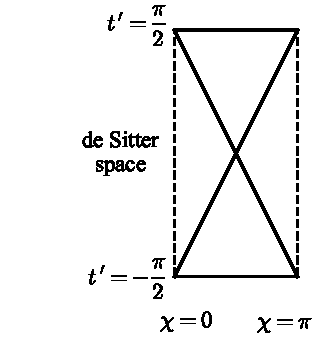
\includegraphics[width=0.72\textwidth]{fig_8.1.pdf}
\caption*{图 8.1\quad de Sitter 时空的共形图。类空切片是三维球面，因此图上的点代表二维球面，只有左右两条边缘上的点除外——它们代表单个点。}
\end{figure}

% ---- 书页 326 / p341 ----
请记住，时空之所以向过去和未来“终结”，仅仅是共形变换的魔力所致；真实的 de Sitter 空间向未来和过去无限延伸。还要注意，两个点可以拥有完全断开的未来（或过去）光锥；这反映了这样一个事实：球状空间截面膨胀得如此之快，以至于来自一点的光永远无法与来自另一点的光相接触。

一个类似的双曲面构造揭示了最大对称而 $\kappa<0$ 的时空，即所谓的 \textbf{反 de Sitter 空间}（anti-de Sitter space）。从一个虚构的五维平直流形出发，其度规为 $\mathrm{d}s_5^2 = -\mathrm{d}u^2 - \mathrm{d}v^2 + \mathrm{d}x^2 + \mathrm{d}y^2 + \mathrm{d}z^2$，并嵌入一个由下式给出的双曲面
\begin{equation*}
-u^2 - v^2 + x^2 + y^2 + z^2 = -\alpha^2.
\tag{8.11}
\end{equation*}
注意这里所有的负号。然后我们可以在双曲面上诱导坐标 $\{t',\rho,\theta,\phi\}$：
\begin{equation*}
\begin{aligned}
u &= \alpha\sin(t')\cosh(\rho)\\
v &= \alpha\cos(t')\cosh(\rho)\\
x &= \alpha\sinh(\rho)\cos\theta\\
y &= \alpha\sinh(\rho)\sin\theta\cos\phi\\
z &= \alpha\sinh(\rho)\sin\theta\sin\phi,
\end{aligned}
\tag{8.12}
\end{equation*}
由此得到这个双曲面上如下形式的度规：
\begin{equation*}
\mathrm{d}s^2 = \alpha^2\left(-\cosh^2(\rho)\,\mathrm{d}t'^2 + \mathrm{d}\rho^2 + \sinh^2(\rho)\,\mathrm{d}\Omega_2^2\right).
\tag{8.13}
\end{equation*}
这些坐标有一个奇怪的特点，即 $t'$ 是周期的。由 (8.12)，$t'$ 与 $t'+2\pi$ 代表双曲面上的同一个位置。由于 $\partial_{t'}$ 处处类时，当 $t'$ 增加时保持 $\{\rho,\theta,\phi\}$ 不变的曲线将是一条闭合类时曲线。然而，这并不是时空的内禀性质，只是我们从特定嵌入导出度规的方式所带来的假象。我们完全可以转而考虑这个流形的“覆盖空间”（covering space），即度规由 (8.13) 给出、但允许 $t'$ 从 $-\infty$ 变到 $\infty$ 的时空。这个空间中没有闭合类时曲线，我们就把这一点取作反 de Sitter 空间的定义。

为了导出共形图，进行一个与 de Sitter 情形类似的坐标变换，不过这次作用在径向坐标上：
\begin{equation*}
\cosh(\rho) = \frac{1}{\cos\chi},
\tag{8.14}
\end{equation*}
于是
\begin{equation*}
\mathrm{d}s^2 = \frac{\alpha^2}{\cos^2\chi}\,\mathrm{d}\bar{s}^2,
\tag{8.15}
\end{equation*}

% ---- 书页 327 / p342 ----
\begin{figure}[H]
\centering
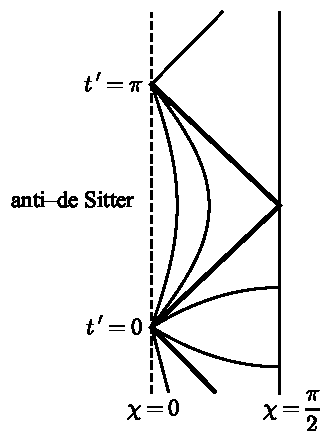
\includegraphics[width=0.72\textwidth]{fig_8.2.pdf}
\caption*{图 8.2\quad 反 de Sitter 时空的共形图。类空切片具有 $\mathbf{R}^3$ 的拓扑，我们用极坐标把它表示出来，因此图上的点代表二维球面，只有左边的点除外——它们代表空间原点处的单个点。无限远是右侧的一个类时曲面。}
\end{figure}

其中 $\mathrm{d}\bar{s}^2$ 表示 Einstein 静态宇宙的度规 (8.9)。与 de Sitter 不同，径向坐标现在出现在共形因子之中。此外，对反 de Sitter 而言，$t'$ 坐标从负无穷一直到正无穷，而径向坐标的范围是
\begin{equation*}
0 \leq \chi < \frac{\pi}{2}.
\tag{8.16}
\end{equation*}
这样，反 de Sitter 空间与 Einstein 静态宇宙的一半共形相关联。其共形图示于图 8.2，图中画出了几条通过点 $t'=0$、$\chi=0$ 的有代表性的类时和类空测地线。由于 $\chi$ 只到 $\pi/2$ 而不是一直到 $\pi$，这个时空的类空切片具有 $S^3$ 中一个半球面内部的拓扑；也就是说，它在拓扑上是 $\mathbf{R}^3$（因而整个时空具有拓扑 $\mathbf{R}^4$）。注意，我们用极坐标画出这张图：左边的一点代表空间原点处的一个点，而右边的一点代表空间无限远处的一个二维球面。另一种流行的表示方法是画出时空的横截面，让空间原点位于正中间，而右边和左边合起来构成空间无限远。

反 de Sitter 的一个有趣特点是，无限远以一个类时超曲面的形式出现，由 $\chi=\pi/2$ 定义。由于无限远是类时的，这个空间不是全局双曲的，我们就没有一个以类空切片上给定的信息来表述的适定初值问题，因为信息总是可以“从无穷远流入”。另一个有趣的特点是，指数映射并不映满整个时空；如图中所画的那样，从指定点出发的测地线并不覆盖整个流形。指向未来的类时测地线，如图所示，起初可以从 $t'=0$、$\chi=0$ 沿径向向外运动，但最终会重新聚焦到点 $t'=\pi$、$\chi=0$，然后再次沿径向向外运动。

% ---- 书页 328 / p343 ----
顺便说一句，我们忍不住要指出：无限远的类时性质促成了弦论的一个引人注目的特征——“AdS/CFT 对应”（AdS/CFT correspondence）。这里 AdS 当然就是我们一直在讨论的反 de Sitter 空间，而 CFT 指的是定义在边界上的共形不变的场论［对 $n$ 维 AdS 来说，这个边界本身就是一个 $(n-1)$ 维时空］。AdS/CFT 对应表明，在某个极限下，AdS 背景上的量子引力（或其超对称版本）与定义在边界上的共形不变的非引力场论之间存在等价关系。关于非引力的量子场论我们知道得很多，而对量子引力却知之甚少，因此这一对应（如果它是正确的——这看起来很有可能，但尚未被证明）将揭示量子引力中可能发生之事的大量信息。\footnote{全面的综述文章见 O.~Aharony, S.S.~Gubser, J.M.~Maldacena, H.~Ooguri, and Y.~Oz, \emph{Phys.\ Rept.} \textbf{323}, 183 (2000), \texttt{http://arxiv.org/hep-th/9905111}。}

于是我们有了三个最大对称的时空：Minkowski（$\kappa=0$）、de Sitter（$\kappa>0$）和反 de Sitter（$\kappa<0$）。它们中有哪一个是真实世界的有用模型吗？进而言之，它们是 Einstein 方程的解吗？先对 (8.1) 给出的 Riemann 张量取迹，并限定到四维：
\begin{equation*}
R_{\mu\nu} = 3\kappa g_{\mu\nu},\qquad R = 12\kappa.
\tag{8.17}
\end{equation*}
可见在最大对称空间中，Ricci 张量与度规成正比。具有这种性质的时空有时被称为 Einstein 空间（Einstein space）；而 Einstein 静态宇宙并\emph{不}是 Einstein 空间的一个例子，这一点有时会令人混淆。更糟的是，我们后面还会遇到 Einstein–de Sitter 宇宙学，它既与 Einstein 空间无关，也与 Einstein 静态宇宙或 de Sitter 空间无关。Einstein 张量为
\begin{equation*}
G_{\mu\nu} = R_{\mu\nu} - \frac{1}{2}Rg_{\mu\nu} = -3\kappa g_{\mu\nu}.
\tag{8.18}
\end{equation*}
因此，Einstein 方程 $G_{\mu\nu}=8\pi G T_{\mu\nu}$ 蕴含（在最大对称时空中如此，并非普遍情形）能量-动量张量与度规成正比：
\begin{equation*}
T_{\mu\nu} = -\frac{3\kappa}{8\pi G}\,g_{\mu\nu}.
\tag{8.19}
\end{equation*}
这样的能量-动量张量对应于真空能或宇宙学常数，如第 4 章所讨论的。能量密度和压强为
\begin{equation*}
\rho = -p = \frac{3\kappa}{8\pi G}.
\tag{8.20}
\end{equation*}
若 $\rho$ 为正，我们得到 de Sitter 解；若 $\rho$ 为负，我们得到反 de Sitter。但在我们的宇宙中，除了可能有真空能之外，还有普通的物质和辐射。我们的最大对称时空并不相容于
% ---- 书页 329 / p344 ----
动力学上可观的物质和/或辐射。此外，由于我们观测到宇宙中的可见物质正在彼此分开（宇宙正在膨胀，下面会讨论），物质的密度在过去更高；所以即使物质对总能量的贡献在今天可以忽略，它在更早的宇宙中也曾经是可观的。因此，最大对称时空并不是真实世界的合理模型。不过，它们确实代表了在没有任何普通物质或引力辐射时 Einstein 方程的（局域）唯一解；正是在这个意义上，它们可以被看作广义相对论的基态。

\section{Robertson–Walker 度规}

为了描述真实世界，我们不得不放弃“完美的”哥白尼原理——它蕴含空间和时间处处都对称——而假定某种更宽容的东西。事实证明，直接假定宇宙在\emph{空间上}均匀且各向同性、但随时间演化，既是直截了当的，又与观测一致。在广义相对论中，这转译为如下陈述：宇宙可以叶状分层（foliated）为一些类空切片，使得每个三维切片都是最大对称的。于是我们把时空取为 $\mathbf{R}\times\Sigma$，其中 $\mathbf{R}$ 代表时间方向，而 $\Sigma$ 是一个最大对称的三维流形。时空度规因此取如下形式
\begin{equation*}
\mathrm{d}s^2 = -\mathrm{d}t^2 + R^2(t)\,\mathrm{d}\sigma^2,
\tag{8.21}
\end{equation*}
其中 $t$ 是类时坐标，$R(t)$ 是一个称为\textbf{尺度因子}（scale factor）的函数，而 $\mathrm{d}\sigma^2$ 是 $\Sigma$ 上的度规，它可以表示为
\begin{equation*}
\mathrm{d}\sigma^2 = \gamma_{ij}(u)\,\mathrm{d}u^i\,\mathrm{d}u^j,
\tag{8.22}
\end{equation*}
其中 $(u^1,u^2,u^3)$ 是 $\Sigma$ 上的坐标，$\gamma_{ij}$ 是一个最大对称的三维度规。尺度因子告诉我们类空切片 $\Sigma$ 在时刻 $t$ 有多大。（不要把它与标量曲率混淆。）这里使用的坐标，其度规没有交叉项 $\mathrm{d}t\,\mathrm{d}u^i$，且 $\mathrm{d}t^2$ 的系数与 $u^i$ 无关，称为\textbf{共动坐标}（comoving coordinates），它是附录 D 讨论的高斯法坐标的一个特例。保持在常数 $u^i$ 处的观者也称为“共动的”。只有共动观者才会认为宇宙看起来是各向同性的；事实上在地球上我们并不完全共动，结果便是我们在宇宙微波背景中看到偶极各向异性，它来源于常规的多普勒效应。

因此我们感兴趣的是最大对称的欧几里得三维度规 $\gamma_{ij}$。我们知道，最大对称的度规满足
\begin{equation*}
{}^{(3)}R_{ijkl} = k\left(\gamma_{ik}\gamma_{jl} - \gamma_{il}\gamma_{jk}\right),
\tag{8.23}
\end{equation*}
其中为了今后的方便我们引入了
\begin{equation*}
k = {}^{(3)}R/6,
\tag{8.24}
\end{equation*}

% ---- 书页 330 / p345 ----
并且在 Riemann 张量上放一个上标 $(3)$，提醒我们它与三维度规 $\gamma_{ij}$ 相联系，而不是与整个时空的度规相联系。Ricci 张量便是
\begin{equation*}
{}^{(3)}R_{jl} = 2k\gamma_{jl}.
\tag{8.25}
\end{equation*}
如果空间要是最大对称的，那它肯定是球对称的。从对 Schwarzschild 解的探索中，我们已经对球对称空间有所了解；度规可以写成
\begin{equation*}
\mathrm{d}\sigma^2 = \gamma_{ij}\,\mathrm{d}u^i\,\mathrm{d}u^j = e^{2\beta(\bar{r})}\,\mathrm{d}\bar{r}^2 + \bar{r}^2\,\mathrm{d}\Omega^2,
\tag{8.26}
\end{equation*}
其中 $\bar{r}$ 是径向坐标，二维球面上的度规一如既往是 $\mathrm{d}\Omega^2 = \mathrm{d}\theta^2 + \sin^2\theta\,\mathrm{d}\phi^2$。这种度规的 Ricci 张量分量可以从 (5.14)——静态球对称时空的 Ricci 张量——通过令 $\alpha=0$ 和 $r=\bar{r}$ 得到，即
\begin{equation*}
\begin{aligned}
{}^{(3)}R_{11} &= \frac{2}{\bar{r}}\,\partial_1\beta\\
{}^{(3)}R_{22} &= e^{-2\beta}\left(\bar{r}\,\partial_1\beta - 1\right) + 1\\
{}^{(3)}R_{33} &= \left[e^{-2\beta}\left(\bar{r}\,\partial_1\beta - 1\right) + 1\right]\sin^2\theta.
\end{aligned}
\tag{8.27}
\end{equation*}
我们利用 (8.25) 令它们与度规成正比，就可以解出 $\beta(\bar{r})$：
\begin{equation*}
\beta = -\frac{1}{2}\ln\left(1-k\bar{r}^2\right),
\tag{8.28}
\end{equation*}
由此得到三维曲面 $\Sigma$ 上的度规
\begin{equation*}
\mathrm{d}\sigma^2 = \frac{\mathrm{d}\bar{r}^2}{1-k\bar{r}^2} + \bar{r}^2\,\mathrm{d}\Omega^2.
\tag{8.29}
\end{equation*}
从 (8.24) 可以注意到，$k$ 的值决定了空间曲面的曲率，从而决定了空间曲面的大小。通常把它归一化，使得
\begin{equation*}
k \in \{+1, 0, -1\},
\tag{8.30}
\end{equation*}
而把流形的物理尺寸吸收进尺度因子 $R(t)$。

$k=-1$ 的情形对应于 $\Sigma$ 上曲率为负的常数，有时称为\textbf{开放}（open）；$k=0$ 的情形对应于 $\Sigma$ 上没有曲率，称为\textbf{平直}（flat）；$k=+1$ 的情形对应于 $\Sigma$ 上曲率为正，有时称为\textbf{闭合}（closed）。引入一个由下式定义的新径向坐标 $\chi$，得到度规的另一种形式，可以使这些情形的物理解释更加清楚：
\begin{equation*}
\mathrm{d}\chi = \frac{\mathrm{d}\bar{r}}{\sqrt{1-k\bar{r}^2}}.
\tag{8.31}
\end{equation*}

% ---- 书页 331 / p346 ----
这可以积分得到
\begin{equation*}
\bar{r} = S_k(\chi),
\tag{8.32}
\end{equation*}
其中
\begin{equation*}
S_k(\chi) \equiv
\begin{cases}
\sin(\chi), & k = +1\\
\chi, & k = 0\\
\sinh(\chi), & k = -1,
\end{cases}
\tag{8.33}
\end{equation*}
于是
\begin{equation*}
\mathrm{d}\sigma^2 = \mathrm{d}\chi^2 + {S_k}^2(\chi)\,\mathrm{d}\Omega^2.
\tag{8.34}
\end{equation*}
对平直情形 $k=0$，$\Sigma$ 上的度规变为
\begin{equation*}
\begin{aligned}
\mathrm{d}\sigma^2 &= \mathrm{d}\chi^2 + \chi^2\,\mathrm{d}\Omega^2\\
&= \mathrm{d}x^2 + \mathrm{d}y^2 + \mathrm{d}z^2,
\end{aligned}
\tag{8.35}
\end{equation*}
这就是平直的欧几里得空间。整体上，它可以描述 $\mathbf{R}^3$ 或者更复杂的流形，比如三维环面 $S^1\times S^1\times S^1$。对闭合情形 $k=+1$，我们有
\begin{equation*}
\mathrm{d}\sigma^2 = \mathrm{d}\chi^2 + \sin^2\chi\,\mathrm{d}\Omega^2,
\tag{8.36}
\end{equation*}
这是三维球面的度规。在这种情形下，唯一可能的整体结构是完全的三维球面（不可定向流形 $\mathbf{RP}^3$ 除外，它由认同 $S^3$ 上的对跖点得到）。最后，对开放的 $k=-1$ 情形，我们得到
\begin{equation*}
\mathrm{d}\sigma^2 = \mathrm{d}\chi^2 + \sinh^2\chi\,\mathrm{d}\Omega^2.
\tag{8.37}
\end{equation*}
这是常负曲率三维空间的度规，是 3.9 节讨论的那个双曲面的推广。整体上，这样的空间可以无限延伸（这正是“开放”一词的由来），但它也可以描述一个非单连通的紧致空间（所以“开放”实在算不上最准确的描述）。

时空的度规描述的正是这些最大对称超曲面之一在尺寸上的演化，它可以写成
\begin{equation*}
\mathrm{d}s^2 = -\mathrm{d}t^2 + R^2(t)\left[\frac{\mathrm{d}\bar{r}^2}{1-k\bar{r}^2} + \bar{r}^2\,\mathrm{d}\Omega^2\right].
\tag{8.38}
\end{equation*}
这就是 \textbf{Robertson–Walker（RW）度规}。我们还没有用到 Einstein 方程；它将决定尺度因子 $R(t)$ 的行为。注意，代换

% ---- 书页 332 / p347 ----
\begin{equation*}
\begin{aligned}
R &\to \lambda^{-1}R\\
\bar{r} &\to \lambda\bar{r}\\
k &\to \lambda^{-2}k
\end{aligned}
\tag{8.39}
\end{equation*}
使 (8.38) 保持不变。因此我们可以选取方便的归一化。在曲率 $k$ 归一化为 $\{+1,0,-1\}$ 的那些变量中，尺度因子具有距离的量纲，而径向坐标 $\bar{r}$（或 $\chi$）实际上是无量纲的；这是最流行的选择。我们偏要反其道而行之，改用无量纲的尺度因子
\begin{equation*}
a(t) = \frac{R(t)}{R_0},
\tag{8.40}
\end{equation*}
一个具有距离量纲的坐标
\begin{equation*}
r = R_0\bar{r},
\tag{8.41}
\end{equation*}
以及一个具有 (长度)$^{-2}$ 量纲的曲率参数
\begin{equation*}
\kappa = \frac{k}{R_0^2}.
\tag{8.42}
\end{equation*}
注意，$\kappa$ 可以取任意值，而不仅仅是 $\{+1,0,-1\}$。在这些变量中，Robertson–Walker 度规为
\begin{equation*}
\boxed{\;\mathrm{d}s^2 = -\mathrm{d}t^2 + a^2(t)\left[\frac{\mathrm{d}r^2}{1-\kappa r^2} + r^2\,\mathrm{d}\Omega^2\right].\;}
\tag{8.43}
\end{equation*}
要转换到更常见的记号，只需代入关系式 (8.40)、(8.41) 和 (8.42)。

有了度规在手，我们就可以着手计算联络系数和曲率张量。令 $\dot{a}\equiv \mathrm{d}a/\mathrm{d}t$，Christoffel 符号为
\begin{equation*}
\begin{array}{ll}
\displaystyle \Gamma^0_{11} = \frac{a\dot{a}}{1-\kappa r^2} & \displaystyle \Gamma^1_{11} = \frac{\kappa r}{1-\kappa r^2}\\[10pt]
\displaystyle \Gamma^0_{22} = a\dot{a}r^2 & \displaystyle \Gamma^0_{33} = a\dot{a}r^2\sin^2\theta\\[6pt]
\displaystyle \Gamma^1_{01} = \Gamma^2_{02} & \displaystyle \Gamma^3_{03} = \frac{\dot{a}}{a}\\[6pt]
\displaystyle \Gamma^1_{22} = -r\left(1-\kappa r^2\right) & \displaystyle \Gamma^1_{33} = -r\left(1-\kappa r^2\right)\sin^2\theta\\[6pt]
\displaystyle \Gamma^2_{12} = \Gamma^3_{13} = \frac{1}{r} & \\[6pt]
\displaystyle \Gamma^2_{33} = -\sin\theta\cos\theta & \displaystyle \Gamma^3_{23} = \cot\theta,
\end{array}
\tag{8.44}
\end{equation*}

% ---- 书页 333 / p348 ----
凡未明确写出的，或者为零，或者由对称性与这些相联系。Ricci 张量的非零分量为
\begin{equation*}
\begin{aligned}
R_{00} &= -3\frac{\ddot{a}}{a}\\[4pt]
R_{11} &= \frac{a\ddot{a} + 2\dot{a}^2 + 2\kappa}{1-\kappa r^2}\\[4pt]
R_{22} &= r^2\left(a\ddot{a} + 2\dot{a}^2 + 2\kappa\right)\\
R_{33} &= r^2\left(a\ddot{a} + 2\dot{a}^2 + 2\kappa\right)\sin^2\theta,
\end{aligned}
\tag{8.45}
\end{equation*}
而 Ricci 标量则为
\begin{equation*}
R = 6\left[\frac{\ddot{a}}{a} + \left(\frac{\dot{a}}{a}\right)^2 + \frac{\kappa}{a^2}\right].
\tag{8.46}
\end{equation*}

\section{弗里德曼方程}

RW 度规对尺度因子 $a(t)$ 的任何行为都有定义；我们的下一步将是把它代入 Einstein 方程，导出把尺度因子与宇宙的能量-动量联系起来的弗里德曼方程（组）（Friedmann equation(s)）。我们将选择用理想流体来模型化物质和能量。显然，如果某种流体在某一个参考系中是各向同性的，而它导致的度规在某一个参考系中是各向同性的，那么这两个参考系将会重合；也就是说，流体在共动坐标中静止。四速度就是
\begin{equation*}
U^\mu = (1, 0, 0, 0),
\tag{8.47}
\end{equation*}
而能量-动量张量
\begin{equation*}
T_{\mu\nu} = (\rho + p)U_\mu U_\nu + pg_{\mu\nu}
\tag{8.48}
\end{equation*}
变为
\begin{equation*}
T_{\mu\nu} = \left(\begin{array}{cccc}
\rho & 0 & 0 & 0\\
0 & & & \\
0 & & g_{ij}p & \\
0 & & &
\end{array}\right).
\tag{8.49}
\end{equation*}
升起一个指标后，它取如下方便的形式：
\begin{equation*}
T^\mu{}_\nu = \mathrm{diag}(-\rho, p, p, p).
\tag{8.50}
\end{equation*}
注意，迹由下式给出：
\begin{equation*}
T = T^\mu{}_\mu = -\rho + 3p.
\tag{8.51}
\end{equation*}
在代入 Einstein 方程之前，先考察能量守恒方程的零分量是有教益的：

% ---- 书页 334 / p349 ----
\begin{equation*}
\begin{aligned}
0 &= \nabla_\mu T^\mu{}_{0}\\
&= \partial_\mu T^\mu{}_{0} + \Gamma^\mu_{\mu\lambda}T^\lambda{}_{0} - \Gamma^\lambda_{\mu 0}T^\mu{}_{\lambda}\\
&= -\partial_0\rho - 3\frac{\dot{a}}{a}\left(\rho + p\right).
\end{aligned}
\tag{8.52}
\end{equation*}
为了取得进展，我们可以选取一个\textbf{物态方程}（equation of state），即 $\rho$ 与 $p$ 之间的一个关系。与宇宙学相关的理想流体常常服从简单的物态方程
\begin{equation*}
p = w\rho,
\tag{8.53}
\end{equation*}
其中 $w$ 是与时间无关的常数。当然，无论它是否保持为常数，我们都可以随意定义参数 $w=p/\rho$；然而，如果 $w$ 在变化，把 $p=w\rho$ 称为“物态方程”就不那么名副其实了。能量守恒方程变为
\begin{equation*}
\boxed{\;\frac{\dot{\rho}}{\rho} = -3(1+w)\frac{\dot{a}}{a}.\;}
\tag{8.54}
\end{equation*}
如果 $w$ 是常数，这可以积分得到
\begin{equation*}
\rho \propto a^{-3(1+w)}.
\tag{8.55}
\end{equation*}
要想了解 $w$ 允许取什么样的值，请参考第 4 章关于能量条件的讨论。类光主能量条件（Null Dominant Energy Condition）允许任何符号的真空能，但除此之外要求物质不能使真空失稳，它蕴含
\begin{equation*}
|w| \leq 1.
\tag{8.56}
\end{equation*}
这个要求绝非不可动摇的金科玉律，但作为研究真实世界中可能发生之事的出发点，它看起来是明智而保守的。

宇宙学流体最流行的两个例子称为\textbf{物质}（matter）和\textbf{辐射}（radiation）。物质是任何一组无碰撞、非相对论性的粒子，其压强基本上为零：
\begin{equation*}
p_{\mathrm{M}} = 0.
\tag{8.57}
\end{equation*}
例子包括普通的恒星和星系，对它们来说，压强与能量密度相比可以忽略。物质也称为尘埃（dust），能量密度主要由物质构成的宇宙称为\textbf{物质主导}的（matter-dominated）。物质中的能量密度按
\begin{equation*}
\rho_{\mathrm{M}} \propto a^{-3}.
\tag{8.58}
\end{equation*}
衰减。这可以直接解释为：随着宇宙膨胀，粒子数密度在减少。对物质而言，能量密度由静能主导，
% ---- 书页 335 / p350 ----
而静能与数密度成正比。辐射既可以描述真实的电磁辐射，也可以描述相对速度足够接近光速、以至于（至少就其物态方程而言）与光子无法区分的有质量粒子。虽然各向同性的相对论性粒子气体是一种理想流体，因而具有由 (8.48) 给出的能量-动量张量，我们也知道，电磁学的 $T_{\mu\nu}$ 可以用场强表达为
\begin{equation*}
T^{\mu\nu} = F^{\mu\lambda}F^{\nu}{}_{\lambda} - \frac{1}{4}g^{\mu\nu}F^{\lambda\sigma}F_{\lambda\sigma}.
\tag{8.59}
\end{equation*}
它的迹由下式给出：
\begin{equation*}
T^\mu{}_\mu = F^{\mu\lambda}F_{\mu\lambda} - \frac{1}{4}(4)F^{\lambda\sigma}F_{\lambda\sigma} = 0.
\tag{8.60}
\end{equation*}
但它也必须等于 (8.51)，所以物态方程为
\begin{equation*}
p_{\mathrm{R}} = \frac{1}{3}\rho_{\mathrm{R}}.
\tag{8.61}
\end{equation*}
能量密度大部分以辐射形式存在的宇宙称为\textbf{辐射主导}的（radiation-dominated）。辐射中的能量密度按
\begin{equation*}
\rho_{\mathrm{R}} \propto a^{-4}.
\tag{8.62}
\end{equation*}
衰减。这样，辐射中的能量密度比物质中的衰减得稍快一些；这是因为光子数密度的减少方式与非相对论性粒子数密度的减少方式相同，但单个光子在红移时还会以 $a^{-1}$ 的方式损失能量，这一点我们稍后会看到。同样，有质量但相对论性的粒子在共动坐标中“慢下来”时也会损失能量。我们相信，今天辐射的能量密度远小于物质的能量密度，$\rho_{\mathrm{M}}/\rho_{\mathrm{R}}\sim 10^{3}$。然而在过去，宇宙要小得多，在极早的时刻，辐射的能量密度本会占据主导。

正如我们讨论过的，真空能也取理想流体的形式，其物态方程为 $p_{\Lambda}=-\rho_{\Lambda}$。其能量密度为常数，
\begin{equation*}
\rho_{\Lambda} \propto a^{0}.
\tag{8.63}
\end{equation*}
由于物质和辐射的能量密度随着宇宙膨胀而减少，如果存在非零的真空能，那么只要宇宙不开始收缩，从长远来看它往往会占上风。如果发生这种情况，我们就说宇宙变得\textbf{真空主导}（vacuum-dominated）。de Sitter 空间和反 de Sitter 空间都是真空主导的解。

现在我们转向 Einstein 方程。回想它可以写成 (4.45) 的形式：
\begin{equation*}
R_{\mu\nu} = 8\pi G\left(T_{\mu\nu} - \frac{1}{2}g_{\mu\nu}T\right).
\tag{8.64}
\end{equation*}
% ==== tail：8.3 节（The Friedmann Equation）收尾，承接书页 335 末的 (8.64)，
% ==== 至书页 337 末止；置于本文件第一个 \section 之前 ====
% ---- 书页 336 / p351 ----
$\mu\nu=00$ 分量方程为
\begin{equation*}
-3\frac{\ddot{a}}{a} = 4\pi G(\rho + 3p),
\tag{8.65}
\end{equation*}
而 $\mu\nu=ij$ 各分量方程给出
\begin{equation*}
\frac{\ddot{a}}{a} + 2\left(\frac{\dot{a}}{a}\right)^{2} + 2\frac{\kappa}{a^{2}} = 4\pi G(\rho - p).
\tag{8.66}
\end{equation*}
由于各向同性，由 $\mu\nu=ij$ 只能得到一个独立的方程。我们可以用式 (8.65) 消去式 (8.66) 中的二阶导数，再稍加整理，得到
\begin{equation*}
\boxed{\,\left(\frac{\dot{a}}{a}\right)^{2} = \frac{8\pi G}{3}\rho - \frac{\kappa}{a^{2}},\,}
\tag{8.67}
\end{equation*}
以及
\begin{equation*}
\boxed{\,\frac{\ddot{a}}{a} = -\frac{4\pi G}{3}(\rho + 3p).\,}
\tag{8.68}
\end{equation*}
这两条方程合称\textbf{弗里德曼方程}（Friedmann equations），而具有式 (8.43) 的形式且满足这些方程的度规，定义了 Friedmann--Robertson--Walker（FRW）宇宙。事实上，如果我们知道 $\rho$ 对 $a$ 的依赖关系，其中第一条式 (8.67) 就足以解出 $a(t)$；当你听到人们提起\emph{那条}弗里德曼方程时，指的就是它，而式 (8.68) 有时被称为\emph{第二}弗里德曼方程。

有一大堆与宇宙学参数相联系的术语，我们在这里只介绍最基本的部分。膨胀的速率由\textbf{Hubble 参量}（Hubble parameter）表征，
\begin{equation*}
\boxed{\,H = \frac{\dot{a}}{a}.\,}
\tag{8.69}
\end{equation*}

% ---- 书页 337 / p352 ----
Hubble 参量在当前时期的值就是 Hubble 常数，$H_0$。目前的测量使我们相信，Hubble 常数为 $70\pm10$ km/sec/Mpc。（Mpc 代表兆秒差距（megaparsec），即 $3.09\times10^{24}$ cm。）由于这个数值仍存在一些不确定性，我们常把 Hubble 常数参数化为
\begin{equation*}
H_0 = 100\,h\ \mathrm{km/sec/Mpc},
\tag{8.70}
\end{equation*}
于是 $h\approx0.7$。典型的宇宙学尺度由\textbf{Hubble 长度}（Hubble length）设定
\begin{align*}
d_H &= H_0^{-1}c \\
&= 9.25\times10^{27}\,h^{-1}\ \mathrm{cm} \\
&= 3.00\times10^{3}\,h^{-1}\ \mathrm{Mpc},
\tag{8.71}
\end{align*}
以及\textbf{Hubble 时间}（Hubble time）
\begin{align*}
t_H &= H_0^{-1} \\
&= 3.09\times10^{17}\,h^{-1}\ \mathrm{sec} \\
&= 9.78\times10^{9}\,h^{-1}\ \mathrm{yr}.
\tag{8.72}
\end{align*}
当然，由于我们通常取 $c=1$，你会看到 $H_0^{-1}$ 既被称作 Hubble 长度，又被称作 Hubble 时间。此外还有\textbf{减速参数}（deceleration parameter），
\begin{equation*}
q = -\frac{a\ddot{a}}{\dot{a}^{2}},
\tag{8.73}
\end{equation*}
它量度膨胀速率的变化速率。

另一个有用的量是\textbf{密度参数}（density parameter），
\begin{equation*}
\boxed{\,\Omega = \frac{8\pi G}{3H^{2}}\rho = \frac{\rho}{\rho_{\mathrm{crit}}},\,}
\tag{8.74}
\end{equation*}
其中\textbf{临界密度}（critical density）定义为
\begin{equation*}
\rho_{\mathrm{crit}} = \frac{3H^{2}}{8\pi G}.
\tag{8.75}
\end{equation*}
这个量一般会随时间变化，被称为\emph{临界}密度，因为弗里德曼方程 (8.67) 可以写成
\begin{equation*}
\Omega - 1 = \frac{\kappa}{H^{2}a^{2}}.
\tag{8.76}
\end{equation*}
因此，$\kappa$ 的符号由 $\Omega$ 大于、等于还是小于 1 决定。我们有
\begin{align*}
\rho < \rho_{\mathrm{crit}} \quad&\leftrightarrow\quad \Omega < 1 \quad\leftrightarrow\quad \kappa < 0 \quad\leftrightarrow\quad \text{开放} \\
\rho = \rho_{\mathrm{crit}} \quad&\leftrightarrow\quad \Omega = 1 \quad\leftrightarrow\quad \kappa = 0 \quad\leftrightarrow\quad \text{平直} \\
\rho > \rho_{\mathrm{crit}} \quad&\leftrightarrow\quad \Omega > 1 \quad\leftrightarrow\quad \kappa > 0 \quad\leftrightarrow\quad \text{闭合}.
\end{align*}
于是，密度参数告诉我们，三种 Robertson--Walker 几何中哪一种描述我们的宇宙。从观测上确定它是至关重要的；近来对宇宙微波背景各向异性的测量使我们相信，$\Omega$ 非常接近于 1。

% ---- 书页 338 / p353 ----

\section{尺度因子的演化}

给定不同组分 $i$ 的能量密度 $\rho_i$ 的数值，连同它们的物态方程 $p_i=p_i(\rho_i)$，以及空间曲率 $\kappa$ 的大小，就可以求解弗里德曼方程 (8.67)，得到尺度因子 $a(t)$ 演化的完整历史。一般来说，我们只需对弗里德曼方程（它只是一阶微分方程）作数值积分，不过，对不同宇宙学参数所对应的解的类型获得一些直观感受是有用的。

为了简化任务，让我们设想能量密度的各个不同组分都按幂律演化，
\begin{equation*}
\rho_i = \rho_{i0}a^{-n_i}.
\tag{8.77}
\end{equation*}
与式 (8.55) 相比较，这等价于假定每个物态方程参数 $w_i=p_i/\rho_i$ 都是一个常数，其值为
\begin{equation*}
w_i = \frac{1}{3}n_i - 1.
\tag{8.78}
\end{equation*}
把空间曲率的贡献当作一种虚构的能量密度（fictitious energy density）来处理，我们还可以进一步简化表达式：
\begin{equation*}
\rho_{\mathrm{c}} \equiv -\frac{3\kappa}{8\pi G a^{2}},
\tag{8.79}
\end{equation*}
以及相应的密度参数
\begin{equation*}
\Omega_{\mathrm{c}} = -\frac{\kappa}{H^{2}a^{2}}.
\tag{8.80}
\end{equation*}
当然，它\emph{不是}能量密度，所以别忘了这只是一种记号上的障眼法。我们最喜欢的几种源的行为总结在下表中。
\begin{equation*}
\begin{array}{l|c|c}
 & w_i & n_i \\ \cline{2-3}
\text{物质} & 0 & 3 \\
\text{辐射} & \frac{1}{3} & 4 \\
\text{曲率} & -\frac{1}{3} & 2 \\
\text{真空} & -1 & 0
\end{array}
\tag{8.81}
\end{equation*}
在这些变量下，弗里德曼方程 (8.67) 可以写成
\begin{equation*}
H^{2} = \frac{8\pi G}{3}\sum_{i(\mathrm{c})}\rho_i,
\tag{8.82}
\end{equation*}
其中记号 $\sum_{i(\mathrm{c})}$ 表示我们不仅对所有真实的能量密度组分 $\rho_i$ 求和，也对空间曲率的贡献

% ---- 书页 339 / p354 ----
$\rho_{\mathrm{c}}$ 求和。注意，如果把两边除以 $H^{2}$，就得到
\begin{equation*}
1 = \sum_{i(\mathrm{c})}\Omega_i.
\tag{8.83}
\end{equation*}
右边的和\emph{不是}总密度参数 $\Omega$，后者只包含来自真实能量密度（不含曲率）的贡献；因此我们有
\begin{equation*}
\Omega_{\mathrm{c}} = 1 - \Omega.
\tag{8.84}
\end{equation*}

让我们先问一问：如果所有的 $\rho_i$（包括 $\rho_{\mathrm{c}}$）都非负，会发生什么。由于 $H^{2}$ 正比于 $\sum_{i(\mathrm{c})}\rho_i$，只要 $\sum_{i(\mathrm{c})}\rho_i\neq0$，宇宙就永远不会经历从膨胀到收缩的转变。我们还可以对 Hubble 参量求时间导数，
\begin{equation*}
\dot{H} = \frac{\ddot{a}}{a} - \left(\frac{\dot{a}}{a}\right)^{2},
\tag{8.85}
\end{equation*}
并代入两条弗里德曼方程 (8.67) 和 (8.68)，得到
\begin{equation*}
\dot{H} = -4\pi G\sum_{i(\mathrm{c})}(1+w_i)\rho_i.
\tag{8.86}
\end{equation*}
由于我们设想 $|w_i|\le1$，当所有 $\rho_i$ 都非负时，我们将总有 $\dot{H}\le0$。换言之，宇宙持续膨胀，但膨胀速率不断减小（这就引出一个绝佳的问题：是什么让宇宙一开始就如此之大？）。

由式 (8.85) 我们看到，$\ddot{a}$ 可以在 $\dot{H}$ 为负的同时为正——即使以 Hubble 参量量度的膨胀速率在减小，尺度因子也可以在“加速”（例如当 $a\propto t^{2}$ 时）。这是非欧几何不可避免的一个微妙之处。Hubble 参量与尺度因子的导数回答的是两个不同的问题。如果把两个检验粒子放在某个固定的初始距离上，问此后很短的时间内它们分开了多少，答案由 Hubble 参量给出；反之，如果选定某个固定的源，问它随时间看上去如何远离我们，答案则由尺度因子的变化给出。因此，“加速”（或“减速”）有两种截然不同但同样正当的含义。实际上，“加速”通常指 $\ddot{a}>0$ 的情形，即使 $\dot{H}<0$。这番讨论并非纯粹学究式的；正如我们在下文将要看到的，我们当前真实的宇宙似乎正是这种类型。

每个 $\rho_i$ 都非负绝非必然。物质和辐射来自动力学的粒子与场，因此我们预期它们的能量密度永远不会为负；如果它们可以为负，空的空间就可能衰变成一团正、负能量的场。但真空和曲率就是另一回事了。真空能是非动力学的，所以负值不会诱发任何不稳定性；而曲率只是空间几何的一种属性，正负皆可。于是，如果我们有
% ---- 书页 340 / p355 ----
负的真空能或正的空间曲率（记住 $\rho_{\mathrm{c}}\propto-\kappa$），Hubble 参量就可以变为零甚至变号。de Sitter 度规 (8.6) 就提供了一个例子：它既有正的真空能，又有正的空间曲率；它描述了一个先坍缩、到达转折点、然后开始膨胀的宇宙。

真实世界是个不整洁的地方，由许许多多不同种类的能量密度组成。不过，由于不同的源以不同的速率演化，在很长一段时间内能量密度会明显地由某一种源主导。因此，考察弗里德曼方程在只有一种能量密度 $\rho\propto a^{-n}$ 时的解是非常有用的。因为我们把空间曲率也当作一种有效的能量源包括进来，这意味着我们要么考虑由单一源主导的平直宇宙，要么考虑具有空间曲率的完全空无一物的宇宙。弗里德曼方程于是意味着
\begin{equation*}
\dot{a}\propto a^{1-n/2}.
\tag{8.87}
\end{equation*}
这可以立即积分得到
\begin{equation*}
\boxed{\,a\propto t^{2/n}\qquad(\text{当 }\rho\propto a^{-n}\text{ 时}).\,}
\tag{8.88}
\end{equation*}
例如考虑一个由物质主导的平直宇宙，$\Omega=\Omega_{\mathrm{M}}=1$；它被称为 Einstein--de Sitter 模型，并且在很长一段时间内曾是描述真实世界的最受青睐的模型（至少在理论家中间是如此）。在 Einstein--de Sitter 宇宙中，尺度因子按 $a\propto t^{2/3}$ 演化；而平直的辐射主导宇宙则按 $a\propto t^{1/2}$ 演化。任何 $n>2$ 的这类宇宙的共形图在附录 H 中导出。尽管我们相信真实宇宙中物质、辐射和真空能的数量都不为零，这些解仍然非常有用；正如我们后面将要讨论的，宇宙在早期是辐射主导的，而在宇宙从 $a\sim1/3000$ 膨胀到 $a\sim1/2$ 的过程中则是物质主导的。

这些解都有一个 $a=0$ 处的奇点，称为\textbf{大爆炸}（Big Bang）。它代表宇宙从奇性状态的创生，而不是物质爆炸进入一个先前存在的时空。人们或许会希望，我们的 FRW 宇宙的完美对称性正是这个奇点的起因，但事实并非如此；宇宙学奇点定理（cosmological singularity theorems）表明，任何满足 $\rho>0$ 且 $p\ge0$ 的宇宙都必定始于一个奇点。当然，当 $a\to0$ 时能量密度变得任意高，我们不指望经典广义相对论在这个区域还能准确地描述自然；想必量子引力将变得重要，尽管目前尚不清楚它如何起作用。

看式 (8.88) 可见，真空能主导（$n=0$）的宇宙显然是一个特例。此时尺度因子按指数而非幂律膨胀；整个度规为
\begin{equation*}
\mathrm{d}s^{2} = -\mathrm{d}t^{2} + e^{Ht}[\mathrm{d}x^{2} + \mathrm{d}y^{2} + \mathrm{d}z^{2}],
\tag{8.89}
\end{equation*}

% ---- 书页 341 / p356 ----
其中 Hubble 参量 $H$ 是常数。当然，在 8.1 节中我们已经描述过一个具有正宇宙学常数的宇宙学时空：de Sitter 空间，其特征是 $\kappa>0$ 且 $a\propto\cosh(t/\alpha)$。那个解与此处 $\kappa=0$、$a\propto\exp(Ht)$ 的解之间是什么关系？它们是同一个时空，只是用不同的坐标来表示。验证这一点的一种办法，是计算 (8.89) 的 Riemann 张量，并检验它具有最大对称时空的特征形式，即式 (8.1)。由于正曲率的最大对称时空在局部是唯一的，度规 (8.6) 与 (8.89) 必定描述同一个流形，或其一部分。实际上，(8.89) 的坐标只覆盖了 de Sitter 空间的一部分；它们在过去是不完备的。在习题中你会被要求证明，这些坐标中的共动测地线会在有限的仿射参量内到达 $t=-\infty$；它们撞上了坐标的边缘。在图 8.1 的共形图中，这些坐标覆盖了正方形右上方的三角形部分。关于 de Sitter 空间和反 de Sitter 空间上各种坐标系的更完备的描述，参见 Hawking and Ellis (1973)。

另一个有趣的特例是 $\rho=0$ 但具有空间曲率的完全空无一物的宇宙。弗里德曼方程变为
\begin{equation*}
H^{2} = -\frac{\kappa}{a^{2}},
\tag{8.90}
\end{equation*}
所以曲率 $\kappa$ 必须为负。把曲率看作一种虚构的能量密度 $\rho_{\mathrm{c}}\propto a^{-2}$，由式 (8.88) 可知，这样的宇宙将线性膨胀，$a\propto t$。这个时空被称为\textbf{Milne 宇宙}（Milne universe）。然而，正如 de Sitter 空间的情形一样，我们知道另一个 $\rho=0$ 的宇宙学时空——在这里就是平直的 Minkowski 空间。再一次，Milne 时空只是 Minkowski 空间在某个不完备坐标系中的一个片。它可以被看作 Minkowski 空间中某个固定点的未来光锥的内部，用负曲率的双曲面来分层。要检验这一点，只需计算 Riemann 张量的所有分量——结果它们全部为零；任何 Riemann 曲率为零的时空在局部都是 Minkowski 空间。

与这些理想化的解相反，一个现实的宇宙学将包含好几种形式的能量-动量。在当前的宇宙中，我们有把握认为辐射密度显著低于物质密度，但真空与物质在动力学上都很重要。因此，方便的做法是用 $\Omega_{\mathrm{M}}$ 和 $\Omega_{\Lambda}$ 来参数化像我们这样的宇宙，曲率则由 $\Omega_{\mathrm{c}}=1-\Omega_{\mathrm{M}}-\Omega_{\Lambda}$ 固定。这类宇宙某些具体例子的膨胀历史示于图 8.3。随着这些宇宙的膨胀，物质、曲率和真空的相对影响会发生变化，因为相应的密度以不同的速率演化：
\begin{equation*}
\Omega_{\Lambda}\propto\Omega_{\mathrm{c}}a^{2}\propto\Omega_{\mathrm{M}}a^{3}.
\tag{8.91}
\end{equation*}
当 $a\to0$ 的过去，曲率和真空将可以忽略，宇宙的行为如同 Einstein--de Sitter。当 $a\to\infty$ 的未来，曲率和物质将可以忽略，宇宙将渐近于 de Sitter 空间；除非尺度因子
% ---- 书页 342 / p357 ----
永远达不到无限大，因为宇宙会在某个有限的时刻开始再度坍缩。

\begin{figure}[H]
\centering
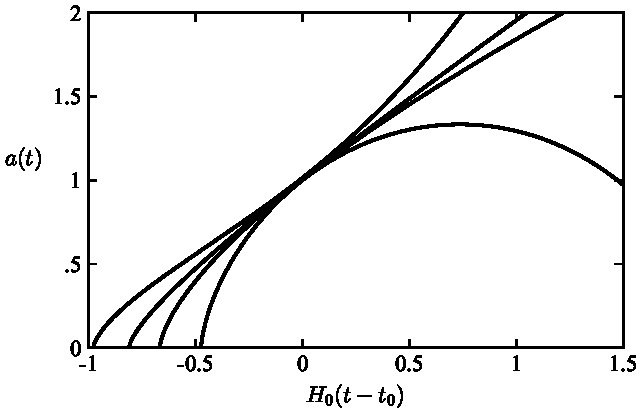
\includegraphics[width=0.72\textwidth]{fig_8.3.pdf}
\caption*{图 8.3\quad 不同 $\Omega_{\mathrm{M}}$ 与 $\Omega_{\Lambda}$ 取值下的膨胀历史。自上而下，各条曲线分别描述 $(\Omega_{\mathrm{M}},\Omega_{\Lambda})=(0.3,0.7)$、$(0.3,0.0)$、$(1.0,0.0)$ 和 $(4.0,0.0)$。}
\end{figure}

如果真空能为负，就\emph{总会}发生再度坍缩；随着宇宙膨胀，真空能最终将占据主导，而 $\Omega_{\Lambda}<0$ 的效果是导致减速和再度坍缩（正如 $\Omega_{\Lambda}>0$ 的效果是把宇宙推开）。当 $\Omega_{\Lambda}\ge0$ 时，如果 $\Omega_{\mathrm{M}}$ 大到足以在 $\Omega_{\Lambda}$ 来得及接管之前使宇宙的膨胀停下来，再度坍缩也是可能的。这些可能性表现为图 8.4 中 $\Omega_{\mathrm{M}}/\Omega_{\Lambda}$ 参数空间的不同区域。对角线代表 $\Omega_{\mathrm{total}}=1$，意味着 $\kappa=0$。

要确定永恒膨胀与最终再度坍缩之间的分界线，请注意：坍缩要求 Hubble 参量在从正变负的过程中经过零。发生这种转折处的尺度因子 $a_{*}$，可以通过在弗里德曼方程中令 $H=0$ 而求得，
\begin{equation*}
H^{2} = 0 = \frac{8\pi G}{3}\left(\rho_{\mathrm{M}0}a_{*}^{-3} + \rho_{\Lambda0} + \rho_{\mathrm{c}0}a_{*}^{-2}\right).
\tag{8.92}
\end{equation*}
把它除以 $H_0^{2}$，利用 $\Omega_{\mathrm{c}0}=1-\Omega_{\mathrm{M}0}-\Omega_{\Lambda0}$，再稍加整理，便得到
\begin{equation*}
\Omega_{\Lambda0}a_{*}^{3} + (1-\Omega_{\mathrm{M}0}-\Omega_{\Lambda})a_{*} + \Omega_{\mathrm{M}0} = 0.
\tag{8.93}
\end{equation*}
（译注：按式 (8.92) 的推导，第二项应为 $\Omega_{\Lambda0}$；原书排印漏写下标 0，原文如此。）

这是关于 $a_{*}$（转折点处的尺度因子）的三次方程。当然，我们对 $a_{*}$ 本身并不很在乎；我们在乎的是，给定 $\Omega_{\mathrm{M}0}$，使 (8.93) 存在实解的 $\Omega_{\Lambda0}$ 值。求解这个三次方程并做一些数学运算，我们发现，宇宙将永远膨胀所对应的 $\Omega_{\Lambda0}$ 值由下式给出

% ---- 书页 343 / p358 ----
\begin{figure}[H]
\centering
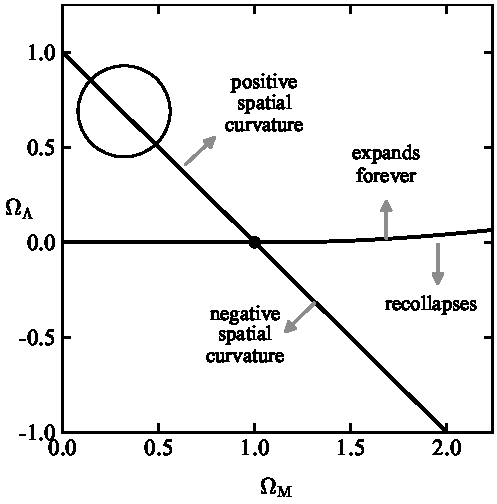
\includegraphics[width=0.72\textwidth]{fig_8.4.pdf}
\caption*{图 8.4\quad 由物质和真空能主导的宇宙的性质，表示为密度参数 $\Omega_{\mathrm{M}}$ 与 $\Omega_{\Lambda}$ 的函数。左上角的圆形区域大致代表实验数据（截至 2003 年）所偏好的数值。}
\end{figure}

\begin{equation*}
\Omega_{\Lambda0} \ge
\left\{
\begin{array}{ll}
0 & 0\le\Omega_{\mathrm{M}0}\le1 \\
4\Omega_{\mathrm{M}0}\cos^{3}\left[\dfrac{1}{3}\cos^{-1}\left(\dfrac{1-\Omega_{\mathrm{M}0}}{\Omega_{\mathrm{M}0}}\right) + \dfrac{4\pi}{3}\right] & \Omega_{\mathrm{M}0}>1.
\end{array}
\right.
\tag{8.94}
\end{equation*}
注意，当 $\Omega_{\Lambda0}=0$ 时，开放和平直宇宙（$\Omega_0=\Omega_{\mathrm{M}0}\le1$）将永远膨胀，而闭合宇宙（$\Omega_0=\Omega_{\mathrm{M}0}>1$）将再度坍缩。对宇宙学常数由来已久的轻视，造成了一种民间信念，认为这是一种必然的对应关系；然而，一旦承认真空能的可能性，空间几何与最终命运之间的任何组合就都是可能的了。

在图 8.4 的左上角，我们标出了目前受偏好的宇宙学参数取值：$\Omega_{\mathrm{M}0}\sim0.3$、$\Omega_{\Lambda0}\sim0.7$，我们将在 8.7 节中讨论。这已深入永恒膨胀的区域；如果真空能保持真正的恒定（它未必如此），我们的宇宙就注定要永远膨胀下去。

在本节的结尾，我们指出为弗里德曼方程寻找静态解的困难。要成为静态，我们必须不仅有 $\dot{a}=0$，还要 $\ddot{a}=0$。由式 (8.68)，这只有在压强为
\begin{equation*}
p = -\frac{1}{3}\rho,
\tag{8.95}
\end{equation*}
时才可能；而由式 (8.67)，还必须存在非零的空间曲率
\begin{equation*}
\frac{\kappa}{a^{2}} = \frac{8\pi G}{3}\rho.
\tag{8.96}
\end{equation*}

% ---- 书页 344 / p359 ----
由于能量密度和压强必须异号，如果我们只诉诸物质或辐射，这些条件就无法满足。当 Einstein 最初在广义相对论中寻找宇宙学解时，天文学家尚未发现宇宙正在膨胀，因此静态解的缺失曾被认为是个难题。这为 Einstein 引入宇宙学常数提供了动机；静态条件可以由物质和真空能的组合来满足，其中
\begin{equation*}
\rho_{\Lambda} = \frac{1}{2}\rho_{\mathrm{M}},
\tag{8.97}
\end{equation*}
再加上适当的正空间曲率。这些参数描述的是\textbf{Einstein 静态宇宙}（Einstein static universe）。如今我们知道宇宙在膨胀，因此这个解没有多少经验上的意义；但它对理论家却极为有用，为共形图的构造提供了基础。

\section{红移与距离}

显然，我们希望通过观测测定若干个量，以判断 FRW 模型中的哪一个对应我们的宇宙。显然我们想测定 $H_0$，因为它与宇宙的年龄有关；我们还想知道 $\Omega$，它通过式 (8.76) 决定 $\kappa$。为了理解这些量究竟可能如何被测量，让我们考虑 FRW 宇宙中的测地线运动。FRW 宇宙中存在若干类空 Killing 矢量，却没有能给我们守恒能量概念的类时 Killing 矢量。不过，确实存在一个 Killing 张量。如果 $U^{\mu}=(1,0,0,0)$ 是共动观者的四速度，那么张量
\begin{equation*}
K_{\mu\nu} = a^{2}(g_{\mu\nu} + U_{\mu}U_{\nu})
\tag{8.98}
\end{equation*}
满足 $\nabla_{(\sigma}K_{\mu\nu)}=0$（你可以自行验证），因而是一个 Killing 张量。这意味着，如果粒子具有四速度 $V^{\mu}=\mathrm{d}x^{\mu}/\mathrm{d}\lambda$，那么
\begin{equation*}
K^{2} = K_{\mu\nu}V^{\mu}V^{\nu} = a^{2}[V_{\mu}V^{\mu} + (U_{\mu}V^{\mu})^{2}]
\tag{8.99}
\end{equation*}
沿测地线将是常数。让我们先就有质量粒子的情形来思考这个问题。此时我们将有 $V_{\mu}V^{\mu}=-1$，于是
\begin{equation*}
(V^{0})^{2} = 1 + |\vec{V}|^{2},
\tag{8.100}
\end{equation*}
其中 $|\vec{V}|^{2}=g_{ij}V^{i}V^{j}$。我们还有 $U_{\mu}V^{\mu}=-V^{0}$，所以式 (8.99) 给出
\begin{equation*}
|\vec{V}| = \frac{K}{a}.
\tag{8.101}
\end{equation*}
因此，随着宇宙膨胀，粒子相对于共动坐标会“慢下来”。事实上这是一种真实的变慢，其意义是：初始相对速度很高的一团粒子气体将随宇宙膨胀而冷却下来。

% ---- 书页 345 / p360 ----
类似的事情也发生在类光测地线上。此时 $V_{\mu}V^{\mu}=0$，式 (8.99) 给出
\begin{equation*}
U_{\mu}V^{\mu} = \frac{K}{a}.
\tag{8.102}
\end{equation*}
但共动观者测得的光子频率是 $\omega=-U_{\mu}V^{\mu}$。因此，以频率 $\omega_{\mathrm{em}}$ 发出的光子，随着宇宙的膨胀将被观测到较低的频率 $\omega_{\mathrm{obs}}$：
\begin{equation*}
\frac{\omega_{\mathrm{obs}}}{\omega_{\mathrm{em}}} = \frac{a_{\mathrm{em}}}{a_{\mathrm{obs}}}.
\tag{8.103}
\end{equation*}
宇宙学家喜欢用这两个事件之间的\textbf{红移}（redshift）$z$ 来谈论它，红移由波长的分数变化定义：
\begin{equation*}
z_{\mathrm{em}} = \frac{\lambda_{\mathrm{obs}} - \lambda_{\mathrm{em}}}{\lambda_{\mathrm{em}}}.
\tag{8.104}
\end{equation*}
如果观测发生在今天（$a_{\mathrm{obs}}=a_0=1$），这意味着
\begin{equation*}
\boxed{\,a_{\mathrm{em}} = \frac{1}{1+z_{\mathrm{em}}}.\,}
\tag{8.105}
\end{equation*}
所以，一个天体的红移告诉我们光子发射时的尺度因子。

注意，这种红移与传统的多普勒效应并不是一回事；导致红移的是空间的膨胀，而不是观者与发射者的相对速度。不过，如果我们在与 Hubble 半径 $H_0^{-1}$ 以及空间曲率半径 $\kappa^{-1/2}$ 相比很小的距离上观测星系，宇宙的膨胀看上去就很像一群星系在彼此远离，红移看上去也很像多普勒效应。因此，天文学家常常用“速度”$v=cz$（$c$ 是光速）来考虑红移。尽管我们知道，对弯曲时空中不同点上的两个物体并不能真正谈论相对速度，但这个虚构的说法在足够短的距离上工作得很好。在这个近似之内，从我们到某个星系的“距离”$d$ 可以取为\textbf{瞬时物理距离}（instantaneous physical distance）$d_P$（即在诸如厘米这样的物理单位下，沿我们当前的空间超曲面量出的、我们与该星系位置之间的距离）。让我们把 RW 度规写成
\begin{equation*}
\mathrm{d}s^{2} = -\mathrm{d}t^{2} + a^{2}(t)R_0^{2}\left[\mathrm{d}\chi^{2} + S_k^{2}(\chi)\,\mathrm{d}\Omega^{2}\right],
\tag{8.106}
\end{equation*}
其中 $S_k(\chi)$ 由式 (8.33) 定义，而 $k\in\{+1,0,-1\}$。在这种形式下，在时刻 $t$ 测得的、我们（$\chi=0$）与共动径向坐标为 $\chi$ 的星系之间的瞬时物理距离就是
\begin{equation*}
d_P(t) = a(t)R_0\chi,
\tag{8.107}
\end{equation*}

% ---- 书页 346 / p361 ----
其中 $\chi$ 保持不变，因为我们假定我们和被观测的星系都完美地共动。（它们可能并不如此；在那种情形下，把所谓“本动速度”（peculiar velocities）引起的修正包括进来是轻而易举的。）当然，“距离”之所以加引号，是因为一旦离开这个近似，就有好几种彼此不等价而有用的距离概念；但当 $d_P$ 很小时它们全都一致。这时，观测到的速度（由红移推断）就简单地是
\begin{equation*}
v = \dot{d}_P = \dot{a}R_0\chi = \frac{\dot{a}}{a}d_P.
\tag{8.108}
\end{equation*}
在今天取值，它就成为
\begin{equation*}
\boxed{\,v = H_0 d_P,\,}
\tag{8.109}
\end{equation*}
这就是著名的\textbf{Hubble 定律}（Hubble law）：对于不太遥远的星系，观测到的退行速度与距离成正比。

如果红移不是非常小，我们就得更仔细地思考宇宙学中“距离”指的是什么。瞬时物理距离是一个方便的构造，但它本身不可观测，因为观测涉及的总是我们过去光锥上的事件，而不是我们当前的空间超曲面。在欧几里得空间中，推断一个物体的距离有许多不同的方法；例如，我们可以把它的视亮度与它的内禀光度相比较，或者把它的视角速度与它的内禀横向速度相比较，或者把它的视角大小与它的物理尺度相比较。对每一种情形，我们都可以定义一种距离，即假如空间是欧几里得的、宇宙不在膨胀时我们\emph{将会}推断出的距离。

让我们从\textbf{光度距离}（luminosity distance）$d_L$ 开始，它的定义是满足
\begin{equation*}
d_L^{2} = \frac{L}{4\pi F},
\tag{8.110}
\end{equation*}
其中 $L$ 是源的绝对光度，$F$ 是观者测得的流量（flux），即单位时间落到某个探测器单位面积上的能量。这个定义来自如下事实：在平直空间中，对位于距离 $d$ 处的源，流量与光度之比正好是以源为中心的球面面积的倒数，$F/L = 1/A(d) = 1/4\pi d^{2}$。然而在 FRW 宇宙中，流量将被稀释。光子数守恒告诉我们，源发出的所有光子最终都将穿过与发射者相距共动距离 $\chi$ 的球面。但流量还会被两个附加效应稀释：单个光子红移一个因子 $(1+z)$；而且光子撞击球面的频率变低，因为相隔 $\delta t$ 发出的两个光子，被观测到的相隔时间是 $(1+z)\delta t$。于是我们将有
\begin{equation*}
\frac{F}{L} = \frac{1}{(1+z)^{2}A}.
\tag{8.111}
\end{equation*}

% ---- 书页 347 / p362 ----
以共动距离 $\chi$ 为中心的球面的面积 $A$，可以从式 (8.106) 中 $\mathrm{d}\Omega^{2}$ 的系数导出，得到
\begin{equation*}
A = 4\pi R_0^{2}S_k^{2}(\chi),
\tag{8.112}
\end{equation*}
其中我们已取 $a(t)=1$，因为我们是在今天观测这些光子。把所有这些合在一起，就得到
\begin{equation*}
d_L = (1+z)R_0S_k(\chi).
\tag{8.113}
\end{equation*}
光度距离 $d_L$ 是我们有希望测量的量，因为有一些天体物理源的绝对光度是已知的。但 $\chi$ 是不可观测的，所以我们必须把它从方程中消去。在类光测地线（为方便起见取为径向）上，我们有
\begin{equation*}
0 = \mathrm{d}s^{2} = -\mathrm{d}t^{2} + a^{2}R_0^{2}\mathrm{d}\chi^{2},
\tag{8.114}
\end{equation*}
即
\begin{equation*}
\chi = R_0^{-1}\int\frac{\mathrm{d}t}{a} = R_0^{-1}\int\frac{\mathrm{d}a}{a^{2}H(a)},
\tag{8.115}
\end{equation*}
其中我们用了 $H=\dot{a}/a$。惯常的做法是用 $a=1/(1+z)$ 把尺度因子换成红移，于是我们有
\begin{equation*}
\chi(z) = R_0^{-1}\int_{0}^{z}\frac{\mathrm{d}z'}{H(z')}.
\tag{8.116}
\end{equation*}

为了计算这个积分中的 Hubble 参量，我们使用弗里德曼方程 (8.67)，像上一节中那样把它写成
\begin{equation*}
H^{2} = \frac{8\pi G}{3}\sum_{i(\mathrm{c})}\rho_i.
\tag{8.117}
\end{equation*}
为了简化问题，我们可以再次假设每个密度组分都按幂律演化，
\begin{equation*}
\rho_i(z) = \rho_{i0}a^{-n_i} = \rho_{i0}(1+z)^{n_i},
\tag{8.118}
\end{equation*}
于是我们可以写出
\begin{equation*}
H(z) = H_0E(z),
\tag{8.119}
\end{equation*}
其中
\begin{equation*}
E(z) = \left[\sum_{i(\mathrm{c})}\Omega_{i0}(1+z)^{n_i}\right]^{1/2},
\tag{8.120}
\end{equation*}

% ---- 书页 348 / p363 ----
其中密度参数 $\Omega_i$ 由式 (8.74) 定义。下面涉及 $E(z)$ 的那些方程，无论能量源是否按幂律演化都成立；若不按幂律演化，只需采用 $E(z)=H(z)/H_0$［其中 $H(z)$ 由弗里德曼方程确定］而不必用式 (8.120)。

于是，光度距离为
\begin{equation*}
d_L(z) = (1+z)R_0S_k\left[R_0^{-1}H_0^{-1}\int\frac{\mathrm{d}z'}{E(z')}\right].
\tag{8.121}
\end{equation*}
注意，当 $k=0$ 时 $R_0$ 自动消去，这很好，因为在那种情形下它是一个完全任意的参数。即使它并非任意，人们通常也更愿意用 $\Omega_{\mathrm{c}0}=-k/R_0^{2}H_0^{2}$ 来讨论；这个量既可以由对空间曲率的测定直接测量，也可以通过测量密度参数并利用 $\Omega_{\mathrm{c}0}=1-\Omega_0$ 来得到。用这个参数，我们有
\begin{equation*}
R_0 = H_0^{-1}\sqrt{-k\Omega_{\mathrm{c}0}} = \frac{H_0^{-1}}{\sqrt{|\Omega_{\mathrm{c}0}|}}.
\tag{8.122}
\end{equation*}
于是，我们把光度距离用可测量的宇宙学参数写成
\begin{equation*}
\boxed{\,d_L(z) = (1+z)\frac{H_0^{-1}}{\sqrt{|\Omega_{\mathrm{c}0}|}}S_k\left[\sqrt{|\Omega_{\mathrm{c}0}|}\int\frac{\mathrm{d}z'}{E(z')}\right].\,}
\tag{8.123}
\end{equation*}
这个方程虽然显得笨拙，却在宇宙学中处于核心地位。给定可观测量 $H_0$ 和 $\Omega_{i0}$，我们可以直接算出到位于任一红移 $z$ 处天体的光度距离；同样地，我们也可以对一系列红移范围内的天体测量 $d_L(z)$，并从这些信息中提取 $H_0$ 和/或各个 $\Omega_{i0}$。

除光度距离之外，还有两个相关的距离量度。正如光度距离是假如我们身处平直空间时，从源的内禀光度和观测光度推断出的距离，\textbf{固有运动距离}（proper motion distance）$d_M$ 是从源的内禀运动和观测运动推断出的距离。它的定义为
\begin{equation*}
d_M = \frac{u}{\dot{\theta}},
\tag{8.124}
\end{equation*}
其中 $u$ 是固有横向速度（比如你会以 k/s 为单位来测量的量），而 $\dot{\theta}$ 是观测到的角速度。另一方面，\textbf{角直径距离}（angular diameter distance）是从源的内禀大小和观测大小推断出的距离；它的定义为
\begin{equation*}
d_A = \frac{R}{\theta},
\tag{8.125}
\end{equation*}

% ==== tail：8.5 节（红移与距离）收尾，承接书页 348 末的 (8.125)，
% ==== 至书页 349 中 8.6 节标题之前；置于本文件第一个 \section 之前 ====

% ---- 书页 349 / p364 ----
%JOIN%其中 $R$ 是天体的固有大小，$\theta$ 是观测到的角直径。在这两种情形下，我们都能导出与式 (8.123) 类似的公式；所幸，对宇宙学参数的那种难以驾驭的依赖关系为所有距离量度所共有，最后剩下的只是对红移的简单依赖：
\begin{equation*}
d_L = (1+z)d_M = (1+z)^{2}d_A,
\tag{8.126}
\end{equation*}
鼓励各位动手验证一下。这样，只要测得了其中一种距离，我们就能方便地换算成其他任何一种；或者，我们也可以独立地测量不同的距离，并利用式 (8.126) 来检验 RW 框架的自洽性。

趁我们还在思量距离，不妨也考虑一下：从红移为 $z$ 的天体发出的光，从发射时刻到现在流逝了多长时间。如果宇宙今天的年龄是 $t_0$，而光子被发射时宇宙的年龄是 $t_{*}$，那么\textbf{回溯时间}（lookback time）为
\begin{align*}
t_0 - t_{*} &= \int_{t_{*}}^{t_0}\mathrm{d}t\\
&= \int_{a_{*}}^{1}\frac{\mathrm{d}a}{aH(a)}\\
&= H_0^{-1}\int_0^{z_{*}}\frac{\mathrm{d}z'}{(1+z')E(z')}.
\tag{8.127}
\end{align*}
例如，考虑一个平直（$k=0$）、物质主导（$\rho=\rho_{\mathrm{M}}=\rho_{\mathrm{M}0}a^{-3}$）的宇宙。那么
\begin{equation*}
E(z) = (1+z)^{3/2},
\tag{8.128}
\end{equation*}
于是
\begin{align*}
t_0 - t_{*} &= H_0^{-1}\int_0^{z_{*}}\frac{\mathrm{d}z'}{(1+z')^{5/2}}\\
&= \frac{2}{3}H_0^{-1}\left[1-(1+z_{*})^{-3/2}\right].
\tag{8.129}
\end{align*}
令 $t_{*}\to 0$（$z_{*}\to\infty$），便得到物质主导宇宙的总年龄：
\begin{equation*}
t_0(\mathrm{MD}) = \frac{2}{3}H_0^{-1}.
\tag{8.130}
\end{equation*}
对于并非完全物质主导的宇宙，$\frac{2}{3}$ 这个因子不会完全正确，但对于合理的宇宙学参数取值，我们通常得到 $t_0\sim H_0^{-1}$。

\section{引力透镜}

在第 7 章中我们介绍了引力透镜（gravitational lensing）的概念：光在 Newton 引力场中的偏折与时间延迟。除了在太阳系内为广义相对论提供检验之外，透镜效应还出现在众多天体物理情境之中，并已成为现代宇宙学不可或缺的组成部分。\footnote{关于引力透镜的一篇优秀综述——我们的讨论即从中借鉴——参见 R.~Narayan and M.~Bartelmann, ``Lectures on Gravitational Lensing,'' 13th Jerusalem Winter School in Theoretical Physics, \texttt{http://arxiv.org/astro-ph/9606001}。}

% ---- 书页 350 / p365 ----
\begin{figure}[H]
\centering
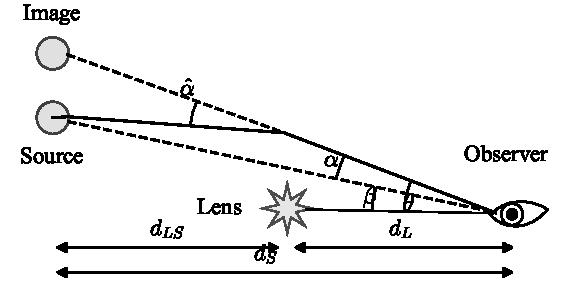
\includegraphics[width=0.72\textwidth]{fig_8.5.pdf}
\caption*{图 8.5\quad 引力透镜的几何，概括于透镜方程 (8.132) 之中。透镜的作用，是把平直 Minkowski 背景中本应观测到的角 $\beta$ 扭变为角 $\theta$。}
\end{figure}

宇宙学透镜效应与我们先前讨论的情形有两个重要区别：Robertson--Walker 度规取代了 Minkowski 背景，而且透镜本身往往也比简单的点质量复杂。图 8.5 描绘了一种典型的透镜几何。在这一节的讨论中，我们将始终假设透镜是“薄”的——即其空间延展尺度远小于源、透镜与观者之间的距离。在这种情形下，我们可以合理地谈论一个唯一的到透镜的距离 $d_L$，以及透镜到源的距离 $d_{LS}$。

对于天空上一幅（可能很复杂的）像，我们用像的不同成分之间的一组夹角来描述它。这些夹角可以看作天空上的二维矢量。透镜的作用，是把没有任何偏折时本应观测到的那些角——例如源与透镜之间的夹角 $\vec{\beta}$——扭变为一幅由一组角 $\vec{\theta}$ 刻画的新像。我们全程假设这些角都很小。这一映射由\textbf{约化透镜角}（reduced lensing angle）$\vec{\alpha}=\vec{\theta}-\vec{\beta}$ 描述。按照图 8.5 所示的几何，它与真实偏转角 $\widehat{\vec{\alpha}}$ 之间的关系为
\begin{equation*}
\vec{\alpha} = \frac{d_{LS}}{d_S}\widehat{\vec{\alpha}}.
\tag{8.131}
\end{equation*}

% ---- 书页 351 / p366 ----
于是我们得到\textbf{透镜方程}（lens equation）
\begin{equation*}
\boxed{\,\vec{\beta} = \vec{\theta} - \frac{d_{LS}}{d_S}\widehat{\vec{\alpha}}.\,}
\tag{8.132}
\end{equation*}
透镜方程所描述的，无非是受扰时空中的光线追踪。

当然，我们应当仔细琢磨图中画出的那些“距离” $d_i$。透镜效应发生在膨胀的宇宙中，而宇宙还可能带有空间曲率。不过，只要我们\emph{定义}距离 $d_i$ 使得透镜方程所描述的几何关系得以成立，透镜方程就依然成立。换言之，这些距离是：在静态欧几里得空间背景中，给定夹角与横向物理尺度时我们本会推断出的距离。而这恰恰就是角直径距离 (8.125) 的定义。因此，本节中的所有距离都取为角直径距离。注意，角直径距离未必能够相加，故 $d_S\neq d_L+d_{LS}$。

举一个简单的例子：点质量透镜。在第 7 章研究 Newton 极限时我们曾经发现，光子穿过引力势 $\Phi$ 时的偏转角由下式给出：
\begin{equation*}
\widehat{\vec{\alpha}} = 2\int \vec{\nabla}_{\perp}\Phi\,\mathrm{d}s,
\tag{8.133}
\end{equation*}
对于碰撞参数为 $b$ 的点质量 $M$，上式化为
\begin{equation*}
\widehat{\vec{\alpha}} = \frac{4GM}{b}.
\tag{8.134}
\end{equation*}
碰撞参数可以写成 $b=d_L\theta$。透镜方程 (8.132) 便成为
\begin{equation*}
\beta = \theta - \frac{d_{LS}}{d_S d_L}\frac{4GM}{\theta}.
\tag{8.135}
\end{equation*}
富有启发性的做法是考虑最简单的情形：源与透镜共线（$\beta=0$）。此时源将被透镜成一个环绕透镜的\textbf{Einstein 环}（Einstein ring），其角距离由\textbf{Einstein 角}（Einstein angle）给出：
\begin{equation*}
\theta_{\mathrm{E}} = \sqrt{\frac{4GMd_{LS}}{d_L d_S}}.
\tag{8.136}
\end{equation*}
即便在更复杂的位形中，Einstein 角也为透镜效应设定了一个特征尺度。我们还可以定义一个与之相联系的距离尺度，即\textbf{Einstein 半径}（Einstein radius）：
\begin{equation*}
R_{\mathrm{E}} = \sqrt{\frac{4GMd_L d_{LS}}{d_S}}.
\tag{8.137}
\end{equation*}

% ---- 书页 352 / p367 ----
换算成厘米或其他物理单位时，别忘了在我们的所有方程中都有 $c=1$。为了对典型天体物理情形下透镜效应的大小有些感觉，我们可以考虑两种常见的场合：我们银河系内近似太阳质量的天体造成的“微透镜”（microlensing），以及星系或星系团造成的宇宙学透镜。前一情形下 Einstein 角将是毫角秒的量级，而后一情形下则是角秒的量级：
\begin{align*}
\theta_{\mathrm{E}} &= 0.9\sqrt{\left(\frac{M}{M_{\odot}}\right)\left(\frac{10\ \mathrm{kpc}}{D}\right)}\ \text{毫角秒}\\
&= 0.9\sqrt{\left(\frac{M}{10^{11}M_{\odot}}\right)\left(\frac{\mathrm{Gpc}}{D}\right)}\ \text{角秒}.
\tag{8.138}
\end{align*}
我们暂时继续讨论点质量透镜。尽管已经观测到若干例壮观的 Einstein 环，但多数时候我们不会幸运到源与透镜恰好完美对齐。这时我们可以求解 (8.135)，得到像角的两个数值：
\begin{equation*}
\theta_{\pm} = \frac{1}{2}\left(\beta \pm \sqrt{\beta^{2}+4\theta_{\mathrm{E}}^{2}}\right).
\tag{8.139}
\end{equation*}
位于 $\theta_{+}$ 处的像总在 Einstein 角之外，而 $\theta_{-}$ 处的像则在其内。实际上这个公式有些误导性：像的数目永远会是奇数；对点质量透镜而言，第三个像将位于与透镜自身相同的位置。

现在来考虑比点质量更一般的透镜。我们知道，偏转角可以借助 Newton 引力势由式 (8.133) 给出。我们可以沿从观者出发指向过去的测地线路径作积分，定义\textbf{透镜势}（lensing potential）：
\begin{equation*}
\psi(\vec{\theta}) = 2\frac{d_{LS}}{d_L d_S}\int \Phi(d_L\vec{\theta},s)\,\mathrm{d}s.
\tag{8.140}
\end{equation*}
利用透镜势，只需取梯度便可直接导出约化透镜角：
\begin{align*}
\vec{\alpha} &= \vec{\nabla}_{\theta}\psi\\
&= 2\frac{d_{LS}}{d_S}\int \vec{\nabla}_{\perp}\Phi\,\mathrm{d}s.
\tag{8.141}
\end{align*}
注意，角梯度 $\vec{\nabla}_{\theta}$ 与 $\vec{\nabla}_{\perp}$（对透镜所在处横向距离的梯度）相差一个因子 $d_L$。薄透镜近似使我们可以把积分收缩为在透镜位置上取值的量。我们还可以对透镜势作用（二维）拉普拉斯算符，得到\textbf{会聚}（convergence）$\kappa$：
\begin{align*}
\kappa(\vec{\theta}) &\equiv \frac{1}{2}\nabla_{\theta}^{2}\psi\\
&= \frac{d_L d_{LS}}{d_S}\int \nabla^{2}\Phi\,\mathrm{d}s.
\tag{8.142}
\end{align*}

% ---- 书页 353 / p368 ----
会聚可以被看作对积分质量密度的一种量度。我们可以把上面的表达式反过来，用会聚同时写出透镜势与约化偏转角：
\begin{equation*}
\psi(\vec{\theta}) = \frac{1}{\pi}\int \kappa(\vec{\theta}\,')\ln|\vec{\theta}-\vec{\theta}\,'|\,\mathrm{d}^{2}\theta'
\tag{8.143}
\end{equation*}
以及
\begin{equation*}
\vec{\alpha}(\vec{\theta}) = \frac{1}{\pi}\int \kappa(\vec{\theta}\,')\frac{\vec{\theta}-\vec{\theta}\,'}{|\vec{\theta}-\vec{\theta}\,'|}\,\mathrm{d}^{2}\theta'.
\tag{8.144}
\end{equation*}
要检验这些方程，请记住这些矢量只定义在两个横向维度上。

会聚描述的是引力透镜对光线的聚焦。这种聚焦使源显得更大（就像放大镜一样）。根据 Liouville 定理——源所发射光子的相空间密度守恒——源的面亮度在透镜作用下保持不变；因此尺度的增大导致亮度的放大。与此同时，光线穿过透镜时的扭转还会引起畸变，导致像的形状发生切变。为了描述这两种现象，我们考虑透镜映射的导数所构成的 $2\times 2$ 矩阵
\begin{equation*}
A_{ij} \equiv \frac{\partial\beta^{i}}{\partial\theta^{j}}.
\tag{8.145}
\end{equation*}
注意，上、下指标之间实际上没有区别，因为它们定义在二维欧几里得平面上。由于 $\vec{\beta}=\vec{\theta}-\vec{\alpha}$，我们有
\begin{align*}
A_{ij} &= \delta_{ij} - \frac{\partial\alpha^{i}}{\partial\theta^{j}}\\
&= \delta_{ij} - \psi_{ij},
\tag{8.146}
\end{align*}
这里我们引入了记号
\begin{equation*}
\psi_{ij} \equiv \frac{\partial^{2}\psi}{\partial\theta^{i}\partial\theta^{j}}.
\tag{8.147}
\end{equation*}
矩阵 $A$ 编码了透镜映射的局域性质。它的逆矩阵被称为\emph{放大张量}（magnification tensor）
\begin{equation*}
\boldsymbol{M} = \frac{\partial\vec{\theta}}{\partial\vec{\beta}} = A^{-1}.
\tag{8.148}
\end{equation*}

% ---- 书页 354 / p369 ----
这个名字从何而来？透镜把由 $\vec{\beta}$ 描述的面元扭变为由 $\vec{\theta}$ 描述的面元，面积的改变由这个映射的雅可比行列式描述，而后者无非是 $\boldsymbol{M}$ 的行列式。这个行列式被定义为\textbf{放大率}（magnification）$\mu$：
\begin{equation*}
\mu = |\boldsymbol{M}| = \frac{1}{|A|}.
\tag{8.149}
\end{equation*}
$\mu$ 的绝对值告诉我们源的亮度实际改变了多少；$\mu$ 可能为负，这意味着像的奇偶性被翻转了。我们说“放大”，是因为只有当透镜和源在天空中彼此靠近时透镜效应才会惹人注意，此时聚焦效应只会带来视亮度的增加；而一个远离源（在天空中位置相距甚远）的透镜所导致的光度极微小的减少，则永远不会被注意到。（如果存在多重像，所有像的亮度之和将超过未畸变源的亮度。）

$A$ 的分量可以分解为会聚与切变的效应。对于会聚，由 $\kappa=\frac{1}{2}\nabla_{\theta}^{2}\psi$ 可得
\begin{equation*}
\kappa = \frac{1}{2}(\psi_{11}+\psi_{22}).
\tag{8.150}
\end{equation*}
而\textbf{切变}（shear）则使源的形状发生畸变；如果初始为圆形的源被畸变为椭圆度为 $\gamma$、方位角为 $\phi$ 的椭圆，我们定义切变的两个分量为
\begin{align*}
\gamma_1 &= \gamma\cos(2\phi)\\
\gamma_2 &= \gamma\sin(2\phi),
\tag{8.151}
\end{align*}
于是总切变为 $\gamma=\sqrt{\gamma_1^{2}+\gamma_2^{2}}$。用透镜势表出，这些分量为
\begin{align*}
\gamma_1 &= \frac{1}{2}(\psi_{11}-\psi_{22})\\
\gamma_2 &= \psi_{12}=\psi_{21}.
\tag{8.152}
\end{align*}
反解这些关系以求出 $A$ 的分量，得到
\begin{equation*}
A = \begin{pmatrix} 1-\kappa-\gamma_1 & -\gamma_2\\ -\gamma_2 & 1-\kappa+\gamma_1 \end{pmatrix}.
\tag{8.153}
\end{equation*}
于是我们可以用会聚与切变来表示放大率：
\begin{equation*}
\mu = \frac{1}{(1-\kappa)^{2}-\gamma^{2}}.
\tag{8.154}
\end{equation*}

% ---- 书页 355 / p370 ----
透镜效应的这些特征在观测宇宙学中正变得日益重要。显然令人感兴趣的是所谓“强透镜”（strong lensing）的情形：源位于透镜的 Einstein 半径之内，这时可能形成多重像。通过观测同一源的多个像，我们可以推断透镜质量分布的性质（例如用来搜寻暗物质）；我们还可以利用不同路径上的时间延迟来测量 Hubble 常数，并利用透镜事件的统计频率来约束其他宇宙学参数。不过，透镜效应不必很强也能产生重要影响。“弱透镜”（weak lensing）——源与透镜相距超过一个 Einstein 半径——一般导致少量的放大与切变，若不预先知道源的性质便无法探测。然而，切变效应可以用统计方法探测：考察成千上万个星系的形状（假定它们的取向本质上是随机的）。弱透镜切变导致这些形状出现相关联的畸变，从而可以揭示观者与遥远源之间物质分布的大量信息。

\section{我们的宇宙}

在讨论 FRW 宇宙学的行为时，我们屡次提及与我们身处的宇宙相对应的宇宙学参数的实际取值。现在让我们更系统一些：既讨论我们今天看到的宇宙，也讨论向早期时刻的合理外推。我们的讨论必然简略，这既出于篇幅考虑，也因为宇宙学是一个活跃的研究领域；想要了解当前观点的最新描述，请查阅近期的综述文章。

我们对膨胀率的许多直接测定，依靠的是把光度距离公式 (8.123) 应用于某种其内禀光度被假定已知的天体，这类天体称为\textbf{标准烛光}（standard candles）。（偶尔我们也测量其内禀尺度被假定已知的物体的角直径：标准尺［standard rulers］。）例如，Hubble 常数就是用各种标准烛光测量的，不同方法达成的共识收敛于前面提到的值 $H_0=70\pm 10$ km/sec/Mpc。高红移处对线性 Hubble 定律 (8.109) 的偏离可以提供关于密度参数 $\Omega_{i0}$ 的信息，但前提是我们必须拥有非常明亮、且内禀光度已被精确掌握的天体。Ia 型超新星（Type Ia supernovae）恰好提供了这样的天体；它们被认为是白矮星吸积了足够多的质量、以至于超过 Chandrasekhar 极限之后发生的爆发。由于 Chandrasekhar 极限接近普适，相应的爆发在本质上亮度相同（而且一部分内禀变化实际上可以通过追踪亮度随时间的演化而加以扣除）。正是在红移 $z>0.3$ 处对 Ia 型超新星的测量，提供了宇宙学常数非零的第一个直接证据；这些观测意味着 $\Omega_{\Lambda}$ 实际上大于 $\Omega_{\mathrm{M}}$。回想一下：物质是无压强的，$p_{\mathrm{M}}=0$，而真空能则伴随着负压强，$p_{\Lambda}=-\rho_{\Lambda}$。代入第二个弗里德曼方程 (8.68)，我们发现一个同时含有物质与 $\Lambda$ 的宇宙服从

% ---- 书页 356 / p371 ----
\begin{equation*}
\frac{\ddot{a}}{a} = -\frac{4\pi G}{3}(\rho_{\mathrm{M}} - 2\rho_{\Lambda}).
\tag{8.155}
\end{equation*}
于是，如果 $\rho_{\Lambda}$ 相对于 $\rho_{\mathrm{M}}$ 足够大（正如超新星观测所表明的），我们就可以有 $\ddot{a}>0$：一个加速膨胀的宇宙（其含义如 8.4 节所述）。

物质密度本身的测量方法多种多样，通常包括通过寻找成团物质的引力效应来测量密度 $\rho_{\mathrm{M}}$，然后再外推到大尺度。由于 $\rho_{\mathrm{M}}=(3H^{2}/8\pi G)\Omega_{\mathrm{M}}$，用这种方式得到的限值常常以 $\Omega_{\mathrm{M}}h^{2}$ 的形式给出，其中 $h$ 定义于式 (8.70)。如今 $H_0$ 的不确定度看来已足够小，取 $h^{2}\approx 0.5$ 相当稳妥，从此以后我们就这么做。当代的大多数方法都与如下结果一致：
\begin{equation*}
\Omega_{\mathrm{M}0} = 0.3\pm 0.1.
\tag{8.156}
\end{equation*}
在宇宙学常数获得充分的观测证据之前，如此低的物质密度有时曾被当作空间负弯曲（$\kappa<0$）的迹象。

除物质与宇宙学常数之外，宇宙中还有辐射。普通光子是辐射密度中最显然的成分，但任何相对论性粒子都会作出贡献。就光子而言，绝大部分能量密度蕴藏于宇宙微波背景——大爆炸遗留下来的辐射——之中。除光子外，辐射成分唯一显然的候选者是中微子。我们预期遗迹背景中微子的数密度与光子相当；光子的数密度可能还要稍大一些，因为在中微子数目固定下来之后，光子仍能继续产生。然而，如果中微子的质量足够大（大于约 $10^{-4}$ eV），它们今天将已经成为非相对论性的，从而对物质而非辐射作出贡献。目前关于中微子质量的看法提示情况很可能如此，但也并非完全清楚。此外，可以设想在我们已知的粒子之外，还存在迄今尚未探测到的无质量粒子（尽管它们不能太多，否则会抑制大尺度结构的形成）。总而言之，总辐射密度看来很可能与光子密度处于同一数量级；在这种情形下我们将有
\begin{equation*}
\Omega_{\mathrm{R}0} \sim 10^{-4}.
\tag{8.157}
\end{equation*}
如前所述，辐射密度低于物质密度并不令人惊讶，因为随着宇宙的膨胀，前者衰减得更快。辐射密度按 $a^{-4}$ 变化，而物质中的密度按 $a^{-3}$ 变化；因此物质-辐射相等发生的红移为
\begin{equation*}
z_{\mathrm{eq}} \approx \frac{\Omega_{\mathrm{M}0}}{\Omega_{\mathrm{R}0}} \sim 3\times 10^{3}.
\tag{8.158}
\end{equation*}

% ---- 书页 357 / p372 ----
对宇宙学参数的另一个关键约束来自微波背景温度的各向异性。平均温度为 $T_{\mathrm{CMB}}=2.74\,\mathrm{K}$，但 1992 年 COBE 卫星发现了随地点起伏、幅度为 $\Delta T/T\sim 10^{-5}$ 的涨落。这些各向异性有多种来源，其中包括复合时光子移出势阱带来的引力红移/蓝移（Sachs--Wolfe 效应，在大角尺度上占主导）、最后散射面上的内禀温度涨落（在小角尺度上占主导），以及等离子体运动的多普勒效应。描写 CMB 各向异性演化的物理超出了本书的范围。整幅天空的 CMB 温度图显然包含大量信息，但没有任何理论预言任意给定点处的温度应该是多少；现代理论预言的，一般是任意给定角尺度上各向异性大小的期望值。因此，我们把各向异性场按球谐函数展开：
\begin{equation*}
\frac{\Delta T}{T}(\theta,\phi) = \sum_{lm} a_{lm}Y_{lm}(\theta,\phi).
\tag{8.159}
\end{equation*}
$|a_{lm}|^{2}$ 的期望值很可能与 $m$ 无关；否则各向异性的统计特性会随天空中的位置而改变（尽管我们对此应当保持开放的心态）。因此，有待测量的相关参数是
\begin{equation*}
C_l = \langle|a_{lm}|^{2}\rangle.
\tag{8.160}
\end{equation*}
由于对任意固定的 $l$，$m$ 有 $2l+1$ 个可能的取值（从 $-l$ 到 $l$），除了最低的几个 $l$ 之外，对 $a_{lm}$ 的独立测量足以精确确定它们的期望值。在非常小的 $l$ 处这种不可约的不确定度被称为宇宙方差（cosmic variance）。

已有大量实验测量了 $C_l$（所谓的 CMB 功率谱），而改进这些测量在今后若干年内很可能仍是一项重要任务。（除温度各向异性之外，CMB 的偏振也包含大量信息，是另一个需要相当多实验努力的目标。）要把这些观测转化为有用的信息，我们需要一个具体的理论来预言 CMB 功率谱如何作为宇宙学参数的函数而变化。有两种领先的可能性（尽管其中一种比另一种要领先得多）：要么密度扰动在极早的时刻就被印记在所有尺度上——甚至包括物理波长 $\lambda$ 远大于 Hubble 半径 $H^{-1}$ 的模式；要么局部的动力学机制在所有时期充当各向异性的源。后一种可能性已基本上被 CMB 数据排除：如果各向异性是连续产生的，我们预期会看到相当平滑、无特征的 $C_l$ 谱，而观测却显示出显著的结构。因此，更流行的做法是设想某种原初的扰动源，例如暴胀（下一节讨论）。暴胀扰动是绝热的——物质密度中的扰动与辐射密度中的扰动相关联——并且在所有尺度上幅度几乎相等。有了这个输入，我们就可以对 $C_l$ 作出作为所有宇宙学参数函数的明确预言。迄今从实验得到的最重要约束或许是：宇宙在空间上是平直的，或至少非常接近平直；$|\Omega_{\mathrm{c}0}|<0.1$。结合物质密度的测量 $\Omega_{\mathrm{M}}\approx 0.3$，我们得出结论：真空能密度参数应为

% ---- 书页 358 / p373 ----
\begin{equation*}
\Omega_{\Lambda 0} = 0.7\pm 0.1.
\tag{8.161}
\end{equation*}
这与上面描述的 Ia 型超新星结果符合得很好；这里描述的调和图像（concordance picture）正是图 8.4 所指示的那一种。利用 $H_0=70$ km/sec/Mpc 把密度参数换算成物理能量密度，得到
\begin{equation*}
\rho_{\mathrm{vac}} \approx 10^{-8}\ \mathrm{erg/cm^{3}},
\tag{8.162}
\end{equation*}
如 4.5 节讨论真空能时所述。

我们的现今宇宙概貌还有一个值得注意的特征。前面提到，我们宇宙中约 $30\%$ 的能量密度由物质组成。但对宇宙学家而言，“物质”是任何非相对论性粒子的集合；我们通过其引力影响推断出的物质，未必是我们在地球上的经验所熟悉的那种普通物质。\textbf{普通物质}（ordinary matter）指由原子及其成分（质子、中子和电子）构成的一切东西；这包括宇宙中所有的恒星、行星、气体和尘埃，无论能否直接看到。这类物质偶尔也被称为\emph{重子物质}（baryonic matter），其中重子包括质子、中子以及相关的粒子（携带一个被称为重子数的守恒量子数的强相互作用粒子）。当然，电子在概念上是普通物质的重要部分，但按质量计算，与质子和中子相比可以忽略：
\begin{gather*}
m_p = 0.938\ \mathrm{GeV}\\
m_n = 0.940\ \mathrm{GeV}\\
m_e = 0.511\times 10^{-3}\ \mathrm{GeV}.
\tag{8.163}
\end{gather*}
换句话说，普通物质的质量绝大部分来自重子。

事实证明，普通的重子物质远不足以解释观测到的密度 $\Omega_{\mathrm{M}}\approx 0.3$。我们目前对重子密度的最佳估计给出
\begin{equation*}
\Omega_{\mathrm{b}} = 0.04\pm 0.02,
\tag{8.164}
\end{equation*}
这些误差限按大多数标准衡量都是保守的。这一测定来自多种方法：直接计数重子（最不精确的方法）、与 CMB 功率谱（上文讨论过）的一致性，以及与大爆炸核合成（下文讨论）对轻元素丰度的预言相符。因此，物质密度的大部分必定采取\textbf{非重子暗物质}（nonbaryonic dark matter）的形式，我们将把它简称为“暗物质”。（重子也可以是暗的，但越来越普遍的用法是把这一术语保留给非重子成分。）粒子物理标准模型中的每一种已知粒子，作为这种暗物质的候选者都已被排除。幸运的是，标准模型之外还有若干看似合理的候选者，包括中性伴随子（neutralino，超对称性所预言的附加稳定粒子中最轻者，质量 $\geq 100$ GeV）和轴子（axion，因假设的 Peccei--Quinn 对称性自发破缺而产生的轻赝标量粒子，引入该对称性是为了解释强相互作用中 CP 的守恒，质量 $\sim 10^{-4}$ eV）。关于暗物质，我们仅有的几点确切认识之一是：它必须是冷的——不仅今天是非相对论性的，而且在很长一段时间里都必须如此。如果暗物质是热的，它就会自由流出高密度区，抑制星系的形成。关于冷暗物质（cold dark matter，CDM）我们知道的另一件事是，它与普通物质的相互作用必须非常微弱，这样才能解释它为何迄今未被探测到。尽管如此，环境中的暗物质粒子偶尔仍可能与地球实验室里经过仔细屏蔽的探测器发生散射；通过搜寻这种散射的效应来直接探测暗物质，将是今后若干年里另一项重要的实验努力。

% ---- 书页 359 / p374 ----
$\Omega_{\mathrm{M}}=0.3$、$\Omega_{\Lambda}=0.7$ 的这幅图像，似乎能拟合种类多得令人印象深刻的观测数据。这幅图中最令人惊讶的部分是宇宙学常数。在第 4 章中我们提到，对真空能的朴素估计给出的结果比测量值大许多个数量级。实际上有三个相互关联的谜题：为什么宇宙学常数比我们预期的小这么多？构成当前宇宙 $70\%$ 的那份小小的非零能量，其起源是什么？还有，为什么真空能的当前值与物质密度处于同一数量级？最后一个问题尤其严峻，因为真空能与物质密度彼此之间演化得很快：
\begin{equation*}
\frac{\Omega_{\Lambda}}{\Omega_{\mathrm{M}}} \propto a^{3}.
\tag{8.165}
\end{equation*}
如果 $\Omega_{\mathrm{M}}$ 和 $\Omega_{\Lambda}$ 今天彼此相当，那么过去真空能会小得探测不到，而将来物质密度将变得可以忽略。这个“巧合问题”（coincidence problem）迄今仍完全是个谜。有人提出的解法涉及“人择原理”（anthropic principle）：如果宇宙存在许多不同的部分（在空间上，甚至在波函数的不同分支上），其中宇宙学常数取非常不同的数值，那么智慧生命最有可能出现在那些绝对值不太大的地方——一个大的正 $\Lambda$ 会在星系形成之前把粒子撕开，而一个大的负 $\Lambda$ 会使宇宙在生命演化出来之前就再度坍缩。对观测到的真空能的人择解释与数据拟合得很好，尽管为解释这一个量就需要求助如此精巧的方案，在一些人看来有点夸张。

另一种可能与巧合问题有关（也可能无关）的想法是：我们探测到的并非非零的宇宙学常数，而是一个紧密切拟真空能性质的动力学成分。对这种可能性的考虑，促使宇宙学家创造了\textbf{暗能量}（dark energy）这个术语，用来称呼无论实际上是什么的被探测到的东西——不管它是动力学的，还是最终被证明就是宇宙学常数。关于暗能量我们知道的是：它在空间中的分布相对平滑（否则它就会像暗物质那样，通过其局部引力场被探测到），并且随时间演化得很慢（否则它就不会像超新星数据所表明的那样使宇宙加速）。暗能量的一个简单的动力学候选者由缓慢滚动的标量场提供。考虑一个具有通常作用量的场 $\phi$：

% ---- 书页 360 / p375 ----
\begin{equation*}
S = \int \mathrm{d}^{4}x\sqrt{-g}\left[-\frac{1}{2}g^{\mu\nu}\nabla_{\mu}\phi\nabla_{\nu}\phi - V(\phi)\right],
\tag{8.166}
\end{equation*}
其能量-动量张量为
\begin{equation*}
T_{\mu\nu} = \nabla_{\mu}\phi\nabla_{\nu}\phi + \left[\frac{1}{2}g^{\rho\sigma}\nabla_{\rho}\phi\nabla_{\sigma}\phi - V(\phi)\right]g_{\mu\nu}
\tag{8.167}
\end{equation*}
而运动方程为
\begin{equation*}
\Box\phi - \frac{\mathrm{d}V}{\mathrm{d}\phi} = 0.
\tag{8.168}
\end{equation*}
假设场在空间中完全均匀（$\partial_i\phi=0$）。于是利用 Christoffel 符号 (8.44)，我们可以用时间导数和 Hubble 常数表示 d'Alembert 算符，把 (8.168) 写成
\begin{equation*}
\ddot{\phi} + 3H\dot{\phi} + \frac{\mathrm{d}V}{\mathrm{d}\phi} = 0.
\tag{8.169}
\end{equation*}
我们看到，Hubble 参量起到摩擦项的作用；场会趋于沿势滚落，但当 $H$ 太大时运动将被阻尼。因此，具有足够平坦的势的标量场（如图 8.6 所绘）将滚动得非常缓慢，导致动能远小于势能 $V(\phi)$。此时能量-动量张量为
\begin{equation*}
T_{\mu\nu} \approx -V(\phi)g_{\mu\nu},
\tag{8.170}
\end{equation*}
\begin{figure}[H]
\centering
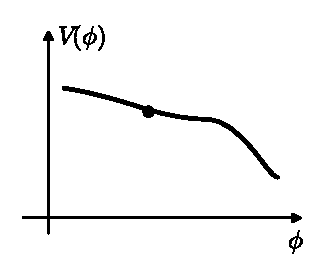
\includegraphics[width=0.72\textwidth]{fig_8.6.pdf}
\caption*{图 8.6\quad 缓慢滚动的标量场的势能。}
\end{figure}
其中 $\phi\approx$ 常数。与式 (4.96) 比较，我们看到标量场势正在摹拟一种真空能。举一个简单的例子，考虑二次势 $V(\phi)=\frac{1}{2}m^{2}\phi^{2}$。这时 (8.169) 描写一个阻尼谐振子，若 $H>m$ 就会出现过阻尼。但在粒子物理单位制中，今天的 Hubble 常数为 $H_0\approx 10^{-33}$ eV，所以这个标量场的质量将不得不比式 (8.163) 中我们熟悉的基本粒子的质量小得难以置信。这看起来像是不自然的微调。尽管如此，动力学暗能量模型正在被积极探索，部分是出于这样的希望：它们能以某种方式通向巧合问题的解决。

% ---- 书页 361 / p376 ----
有了对当代状况的这一认识，我们就可以设想，早期宇宙必须是什么样子，才能产生出我们今天看到的一切。为了物理直观，标记所考虑的时代时，用温度来表示往往比用红移或大爆炸以来的时间更有帮助。今天的温度是
\begin{equation*}
T_0 = 2.74\ \mathrm{K} = 2.4\times 10^{-4}\ \mathrm{eV}.
\tag{8.171}
\end{equation*}
当然，这里说“温度”，我们指的是宇宙微波背景的表观黑体温度；实际上 CMB 自复合以来就不再处于热平衡，所以对这个概念不宜过分当真。在绝热膨胀下，随着每种相对论性粒子红移，温度都在下降，我们有 $T\propto a^{-1}$。但在早期宇宙的特定时刻会发生非绝热相变；在这种情形下温度实际上并不会升高，只是下降得更加缓慢。为了帮助建立温度、密度与尺度因子之间的关系，我们引入\textbf{相对论性自由度的有效数目}（effective number of relativistic degrees of freedom）的两种不同量度：$g_{*}$ 与 $g_{*S}$（其中 $S$ 代表熵）。考虑一组玻色子与费米子物种，每一种都有自己的有效温度 $T_i$ 和自旋态数目 $g_i$。例如，无质量光子有两个自旋态，故 $g_{\gamma}=2$；有质量的 $\frac{1}{2}$ 自旋费米子也有两个自旋态，故 $g_{e^-}=g_{e^+}=2$。相对论性自由度有效数目的这两个不同版本满足
\begin{equation*}
g_{*} = \sum_{\mathrm{bosons}} g_i\left(\frac{T_i}{T}\right)^{4} + \frac{7}{8}\sum_{\mathrm{fermions}} g_i\left(\frac{T_i}{T}\right)^{4}
\tag{8.172}
\end{equation*}
而
\begin{equation*}
g_{*S} = \sum_{\mathrm{bosons}} g_i\left(\frac{T_i}{T}\right)^{3} + \frac{7}{8}\sum_{\mathrm{fermions}} g_i\left(\frac{T_i}{T}\right)^{3}.
\tag{8.173}
\end{equation*}
神秘的 $\frac{7}{8}$ 因子，来源于计算平衡分布函数时玻色统计与费米统计的差别。对任何处于热平衡的物种，其温度 $T_i$ 将等于背景温度 $T$；但也可能有物种在更低的温度下就已退耦，它们对相对论性自由度有效数目的贡献较小。之所以需要定义两种不同的量度，是因为它们扮演的角色不同：第一个通过
\begin{equation*}
\rho_{\mathrm{R}} = \frac{\pi^{2}}{30}g_{*}T^{4},
\tag{8.174}
\end{equation*}
把温度与（相对论性物种的）能量密度联系起来，
而第二个则把温度与尺度因子联系起来：
\begin{equation*}
T \propto g_{*S}^{-1/3}a^{-1}.
\tag{8.175}
\end{equation*}

% ==== tail：8.7 节（Our Universe）的收尾文字，承接书页 361 末的式 (8.175) 之后的段落，
% ==== 至本文件第一个 \section（8.8 暴胀）之前；由装配器移至 ch8_c 之后 ====

% ---- 书页 362 / p377 ----
事实上，只要相对论性自由度还是粒子物理标准模型中的那些，$g_{*}$ 与 $g_{*S}$ 就应当近似相等。一个十分粗略的估算指南是
\begin{equation*}
g_{*} \approx g_{*S} \sim
\left\{
\begin{array}{ll}
100 & T > 300~\mathrm{MeV} \\
10 & 300~\mathrm{MeV} > T > 1~\mathrm{MeV} \\
3 & T < 1~\mathrm{MeV}.
\end{array}
\right.
\tag{8.176}
\end{equation*}
正如我们马上就要讨论的，改变相对论性自由度有效数目的事件，是 $300~\mathrm{MeV}$ 处的 QCD 相变，以及 $1~\mathrm{MeV}$ 处电子/正电子对的湮灭。

有了这些背景，让我们来考虑宇宙从早期到今天的演化。作为开始，我们想象一个 Robertson--Walker 度规，其物质场处于温度 $1~\mathrm{TeV}=1000~\mathrm{GeV}$ 的热平衡中。高温等离子体是基本粒子（夸克、轻子、规范玻色子和 Higgs 玻色子）的复杂混合物。能量密度的主导形式将是相对论性粒子，因此早期宇宙是辐射主导的。它还非常接近平直，因为弗里德曼方程中的曲率项比物质密度和辐射密度演化得更慢。于是弗里德曼方程为
\begin{equation*}
\begin{aligned}
H^{2} &= \frac{8\pi G}{3}\rho_{\mathrm{R}} \\
&\approx 0.1\,g_{*}\,\frac{T^{4}}{\bar{m}_{\mathrm{P}}^{2}},
\end{aligned}
\tag{8.177}
\end{equation*}
其中约化 Planck 标度为 $\bar{m}_{\mathrm{P}}=(8\pi G)^{-1/2}\approx 10^{18}~\mathrm{GeV}$。如果辐射主导的阶段一直延伸到极早期，宇宙的年龄将近似为 $t\sim H^{-1}$，即
\begin{equation*}
t \sim \frac{\bar{m}_{\mathrm{P}}}{T^{2}}.
\tag{8.178}
\end{equation*}
用常规单位表示，这变为
\begin{equation*}
t \sim 10^{-6}\left(\frac{\mathrm{GeV}}{T}\right)^{2}~\mathrm{sec}.
\tag{8.179}
\end{equation*}

目前粒子加速器上的实验已经为大约 $100~\mathrm{GeV}$ 以下的物理图景提供了准确的描述，因此再外推一个数量级仍属于合理外推的范围。在更高的温度下我们就不太确定会发生什么了；在 $1~\mathrm{TeV}$ 和 Planck 标度之间也许没有任何非常有趣的事情，也可能这个区域充满了各式各样的意外。当然，也可以设想宇宙学在更低的温度下就会给出意外，尽管标准模型物理已被理解得很透彻；本节我们描述的是一个保守的方案，但一如既往，保持开放的头脑总是值得的。

% ---- 书页 363 / p378 ----
标准模型的一个关键特征是电弱部分的自发破缺对称性。在宇宙学中，这种对称性破缺发生在电弱相变处，温度 $T\sim 200~\mathrm{GeV}$。在此温度之上对称性尚未破缺，因此基本费米子（夸克和轻子）与弱相互作用规范玻色子都无质量；在此温度之下，我们便得到低能实验所熟知的那些质量模式。电弱相变预计不会给晚期宇宙留下任何可察觉的影响；一个可能的例外是重子生成（baryogenesis），下面讨论。

在这些温度下，量子色动力学（QCD）所描述的强相互作用并不那么强。在低能量/温度下，QCD 表现出“禁闭”（confinement）——夸克和胶子被束缚成重子和介子这样的复合粒子。但在 QCD 标度 $\Lambda_{\mathrm{QCD}}\sim 300~\mathrm{MeV}$ 之上，夸克和胶子是自由粒子。随着宇宙膨胀和冷却，强相互作用粒子被禁闭成束缚态，这正是 (8.176) 中所指出的相对论性自由度有效数目第一次下降的原因。QCD 相变预计不会在可观测宇宙上留下显著的印记。

正如强相互作用在高温下并不很强，弱相互作用也不像你可能以为的那么弱；它们仍然是弱的——在微扰论能够准确描述的意义上——但其发生得足够快，足以使中微子这类弱相互作用粒子保持在热平衡中。当 $T\sim 1~\mathrm{MeV}$ 时，情况不再如此。这也大致是电子和正电子变为非相对论性并发生湮灭的温度，相对论性自由度的有效数目因此减少，但这两件事互不相干。对 $1~\mathrm{MeV}$ 以下的温度，我们说弱相互作用已经“冻结”（frozen out）——相互作用速率降到宇宙的膨胀速率之下，相互作用发生得过于稀少，无法再使粒子保持平衡。冷暗物质粒子有可能就是在这个温度从等离子体中退耦的。更有把握的是，我们可以断定中子和质子不再相互转换。在这个温度下中子的平衡丰度约为质子丰度的 $1/6$（因为中子的质量稍大）。中子的寿命有限（$\tau_{n}=890~\mathrm{sec}$），只比这个时期宇宙的年龄 $t(1~\mathrm{MeV})\approx 1~\mathrm{sec}$ 略长，但它们已开始逐渐衰变为质子和轻子。然而不久之后，我们就到达略低于 $100~\mathrm{keV}$ 的温度，\textbf{大爆炸核合成}（Big-Bang Nucleosynthesis，BBN）开始了。

每个核子的核结合能典型地为 $1~\mathrm{MeV}$ 的量级，所以你也许会以为核合成应该更早发生；然而，每个核子对应的光子数太多，阻碍了核合成的发生，直到温度降到 $100~\mathrm{keV}$ 以下。在那一点上，中子/质子比约为 $1/7$。在所有轻核之中，核子驻留在 $^{4}\mathrm{He}$ 里在能量上是有利的，事实上大多数自由中子也确实被转化成了 $^{4}\mathrm{He}$；每两个中子和十四个质子，最终得到一个氦核和十二个质子。于是，按质量计约有 $25\%$ 的重子被转化为氦。此外，还有痕量的氘（每质子约 $10^{-5}$ 个氘核）、$^{3}\mathrm{He}$（同样约 $10^{-5}$）以及 $^{7}\mathrm{Li}$（约 $10^{-10}$）。

% ---- 书页 364 / p379 ----
当然，这些数字是预言，而它们确实被对轻元素原初丰度的观测所证实。（更重的元素并非在大爆炸中合成，而是需要晚期宇宙中的恒星过程。）我们对许许多多关键细节作了粗略带过，尤其是那些解释各种丰度如何依赖宇宙学参数的细节。例如，设想我们偏离标准模型，引入三种以上的轻中微子物种。这会通过式 (8.174) 在固定温度下增大辐射能量密度，转而又缩短了与给定温度相联系的时标（因为 $t\sim H^{-1}\propto\rho_{\mathrm{R}}^{-1/2}$）。核合成因此会稍早发生，导致中子丰度更高，从而 $^{4}\mathrm{He}$ 丰度也更大。对原初氦丰度的观测与标准模型的预言相符，给出了轻中微子数目接近三的第一个证据。类似地，与核合成相联系的所有温度和时标都依赖于重子/光子比；要与观测到的丰度相符，就要求每光子大约有 $5\times 10^{-10}$ 个重子，这正是重子密度参数之估计值 (8.164) 的由来，以及随之而来的对非重子暗物质的需要。

就我们当下的目的而言，原初核合成最深刻的特征，也许是它对温度与膨胀率之间的弗里德曼关系——从而对 Einstein 方程——的敏感依赖。BBN 的成功为 GR 提供了一个在远离我们日常经验的领域中的严格检验。Einstein 的理论当初被提出，主要是出于把引力与电磁学的洛伦兹对称性不变性相协调的需要；而这样一个理论竟能成功描述宇宙仅一秒钟大小时的增长，这实在是令人赞叹的成就。时至今日，BBN 仍是对各种替代引力理论最强有力的约束之一；特别地，它是我们拥有任何直接观测特征的最早时期。

核合成之后，我们得到一个由质子、电子和光子主导的等离子体，其中还有一些氦和其他核。也有暗物质存在，但假定到这个时期它已不与普通物质相互作用。下一个重要事件直到\textbf{复合}（recombination）才发生：电子与质子结合（它们与氦的结合稍早一些）。复合发生在温度 $T\approx 0.3~\mathrm{eV}$；此时宇宙是物质主导的。同样地，由于氢的结合能是 $13.6~\mathrm{eV}$，你也许会以为复合应该更早发生，但巨大的光子/重子比把它推迟了。复合至关重要的意义在于，它标志着宇宙变得透明的时刻。环境光子与自由电子强烈地相互作用，因此在复合之前光子的平均自由程非常短；而一旦电子和质子结合成中性氢，平均自由程实际上就变成了无穷大。这些环境光子今天作为宇宙微波背景被我们看到，它提供了宇宙在 $T\approx 0.3~\mathrm{eV}$ 时、即红移 $z\approx 1200$ 时的一幅快照。复合是一个颇为渐进的过程，因此对它发生于何时所作的任何指定都必然是近似的。

% ---- 书页 365 / p380 ----
复合之后，宇宙要走过一段被称为“黑暗时代”（dark ages）的漫长时期，其间星系通过引力不稳定性逐渐集结起来，但还没有可见的恒星来照亮宇宙。黑暗时代是一个神秘的时期；恒星和星系形成的过程高度复杂且非线性，无疑需要新类型的观测，我们才能对这一时代有充分的理解。

我们的故事现在已经把我们带到了今天，但还有几个缺失的环节需要回过头来补上。其一是宇宙中物质与反物质之间的不对称。宇宙中基本上全部可见物质似乎都由质子、中子和电子构成，而非它们的反粒子；如果遥远的星系主要由反物质构成，我们就应当能观测到物质/反物质区域边界处质子与反质子偶尔湮灭所产生的高能光子。虽然可以把这种不对称作为初始条件硬性加进去，但这总显得有些不能令人满意，大多数物理学家更愿意找到某种重子生成的动力学机制，让一个初始时物质/反物质对称的态演化成我们今天的宇宙。这样的破缺对称在粒子物理中很常见，事实上人们已经提出了许多重子生成机制（通常在电弱标度或更高的温度下）。然而，这些具体方案中没有一个已被证明足够令人信服而被采纳为标准方案。要理解重子不对称的起源，我们很可能需要对超越标准模型的物理有更好的理解。

另一个需要提及的缺失特征是，宇宙当然并非完全均匀和各向同性；宇宙中目前的大尺度结构似乎演化自极早期就存在的、幅度为 $\delta\rho/\rho\sim 10^{-5}$ 的绝热且近无标度微扰。这些微扰的绝热性和近无标度性的证据，来自对 CMB 和大尺度结构的联合观测。高度的各向同性和均匀性，以及对其的小偏离，在传统宇宙学中都只是作为神秘的初始条件被强加上去的。暴胀宇宙方案（inflationary-universe scenario）为两者提供了一个可能的动力学起源，我们现在就转向它。

\section{暴胀}

在对大爆炸模型的传统理解中，宇宙被认为在早期是辐射主导的，在晚期是物质主导的，而且——正如我们现在怀疑的——在非常晚近的时候才转变为真空主导。这幅图像在描述形形色色的观测数据方面取得了巨大成功；尽管如此，我们仍然可以问，产生这样一个宇宙的初始条件是否显得自然。这是那种人们在宇宙学中会问、在其他科学中却不会问的问题。通常，作为物理学家，我们寻找自然定律，并想象我们可以自由地指定初始条件，然后问它们在这些定律下如何演化。但宇宙似乎只有一组初始条件，因此，想知道它们究竟是相对平常的还是经过精细调节的，似乎是合情合理的。

% ---- 书页 366 / p381 ----
在传统图像中，早期宇宙确实被精细调节到了难以置信的精度。特别是，我们宇宙的两个特征看上去非常不寻常：它的空间平直性，以及它高度的各向同性和均匀性。有可能这就是我们恰好被给予的宇宙，追问不同初始条件的可能性有多大毫无意义；另一种可能是，如果存在某种动力学机制，能把宽广谱系的初始条件朝平直性和均匀性/各向同性的方向演化，那么这些条件就比乍看之下更有可能出现。暴胀宇宙方案提供了这样一种机制（而且还不止如此），它已成为现代宇宙学的核心组织原理，即使我们还远不能证明它的正确性。

在描述暴胀之前，让我们先描述它声称解决的两个不自然性问题：与均匀性/各向同性相联系的\textbf{平坦性问题}（flatness problem）和\textbf{视界问题}（horizon problem）。平坦性问题来自考虑一个有物质和辐射但没有真空能的宇宙中的弗里德曼方程；为方便后文，我们用约化 Planck 质量 $\bar{m}_{\mathrm{P}}=(8\pi G)^{-1/2}$ 把它写成
\begin{equation*}
H^{2} = \frac{1}{3\bar{m}_{\mathrm{P}}^{2}}\left(\rho_{\mathrm{M}}+\rho_{\mathrm{R}}\right) - \frac{\kappa}{a^{2}}.
\tag{8.180}
\end{equation*}
曲率项 $-\kappa/a^{2}$ 与 $a^{-2}$ 成正比（这显而易见），而能量密度项随尺度因子的增大衰减得更快，$\rho_{\mathrm{M}}\propto a^{-3}$、$\rho_{\mathrm{R}}\propto a^{-4}$。这就引出了一个问题：考虑到自 Planck 时期以来 $a$ 已经增大了大约 $10^{30}$ 倍，为什么比值 $(\kappa a^{-2})/(\rho/3\bar{m}_{\mathrm{P}}^{2})$ 没有远远大于 1？换句话说，在物质/辐射主导的宇宙中，$\Omega=1$ 这个点是一个排斥性的不动点——对这个值的任何偏离都会随时间增长，那么为什么我们今天观测到的是 $\Omega\approx 1$？

视界问题源于 FRW 宇宙学中粒子视界的存在，如图 8.7 所示。视界之所以存在，是因为自大爆炸奇点以来只有有限的时间，因而在宇宙的年龄之内光子只能走过有限的距离，正如我们在第 2 章中简要讨论过的。考虑在平直宇宙中沿径向轨迹运动的一个光子（推广到非平直宇宙是直截了当的）。径向类光路径满足
\begin{equation*}
0 = \mathrm{d}s^{2} = -\mathrm{d}t^{2} + a^{2}\mathrm{d}r^{2},
\tag{8.181}
\end{equation*}
因此这样的一个光子在 $t_{1}$ 与 $t_{2}$ 两时刻之间走过的共动（坐标）距离为
\begin{equation*}
\Delta r = \int_{t_{1}}^{t_{2}}\frac{\mathrm{d}t}{a(t)}.
\tag{8.182}
\end{equation*}
要得到任一时刻 $t$ 处观者所测得的物理距离，只需乘上 $a(t)$。为简单起见，让我们想象自己处在一个物质主导的
% ---- 书页 367 / p382 ----
宇宙，对它而言
\begin{equation*}
a = \left(\frac{t}{t_{0}}\right)^{2/3}.
\tag{8.183}
\end{equation*}
\begin{figure}[H]
\centering
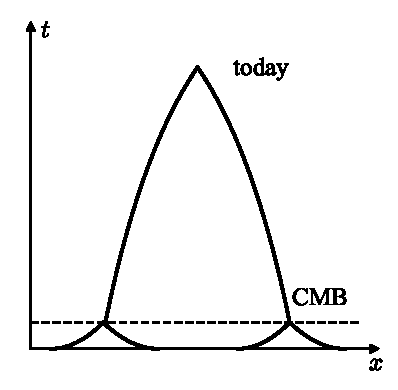
\includegraphics[width=0.72\textwidth]{fig_8.7.pdf}
\caption*{图 8.7\quad 从一个由大爆炸奇点膨胀而来的宇宙中的过去光锥，展示了宇宙学中的粒子视界。处于复合时刻的一些点——今天作为天空中相反两侧的宇宙微波背景被我们观测到——其过去光锥互不重叠（在传统宇宙学中）；没有任何因果信号能够影响它们，使它们具有相同的温度。}
\end{figure}
记住 $a_{0}=1$。因此 Hubble 参量为
\begin{equation*}
\begin{aligned}
H &= \frac{2}{3}t^{-1} \\
&= a^{-3/2}H_{0}.
\end{aligned}
\tag{8.184}
\end{equation*}
于是该光子走过的共动距离为
\begin{equation*}
\Delta r = 2H_{0}^{-1}\left(\sqrt{a_{2}}-\sqrt{a_{1}}\right).
\tag{8.185}
\end{equation*}
在尺度因子取任一固定值 $a=a_{*}$ 时的共动视界尺度，是光子自大爆炸以来走过的距离，
\begin{equation*}
r_{\mathrm{hor}}(a_{*}) = 2H_{0}^{-1}\sqrt{a_{*}}.
\tag{8.186}
\end{equation*}
而在 $a_{*}$ 处的空间超曲面上测得的物理视界尺寸，因此就简单地是
\begin{equation*}
d_{\mathrm{hor}}(a_{*}) = a_{*}r_{\mathrm{hor}}(a_{*}) = 2H_{*}^{-1}.
\tag{8.187}
\end{equation*}
事实上，对任何包含物质和辐射混合物的近平直宇宙，在任一给定时期我们都有
\begin{equation*}
d_{\mathrm{hor}}(a_{*}) \sim H_{*}^{-1} = d_{H}(a_{*}),
\tag{8.188}
\end{equation*}

% ---- 书页 368 / p383 ----
其中 Hubble 距离 $d_{H}$ 已在式 (8.71) 中引入。这种近似相等带来一种强烈的诱惑，即把“视界距离”和“Hubble 距离”当作同义词使用；这种诱惑应当抵制，因为暴胀可以使前者远大于后者，我们很快就会证明这一点。

视界问题简单说来就是：CMB 在很高的精度上是各向同性的，尽管最后散射面上相距遥远的各点彼此完全处于对方的视界之外。当我们观看 CMB 时，我们观测的是尺度因子 $a_{\mathrm{CMB}}\approx 1/1200$ 处的宇宙；由式 (8.185)，CMB 上一点与地球上的观者之间的共动距离为
\begin{equation*}
\begin{aligned}
\Delta r &= 2H_{0}^{-1}\left(1-\sqrt{a_{\mathrm{CMB}}}\right) \\
&\approx 2H_{0}^{-1}.
\end{aligned}
\tag{8.189}
\end{equation*}
然而，这样一个点所对应的共动视界距离为
\begin{equation*}
\begin{aligned}
r_{\mathrm{hor}}(a_{\mathrm{CMB}}) &= 2H_{0}^{-1}\sqrt{a_{\mathrm{CMB}}} \\
&\approx 6\times 10^{-2}H_{0}^{-1}.
\end{aligned}
\tag{8.190}
\end{equation*}
因此，如果我们观测 CMB 中相距遥远的两个部分，它们的视界将互不重叠；CMB 天空中不同的斑块在复合时刻是因果不连通的。然而，观测却表明它们具有相同的温度，且精度很高。于是问题就来了：既然它们从未处于因果接触之中，它们是如何预先知道要以正确的方式协调各自的演化的？我们必须设法修正传统 FRW 宇宙学的因果结构。

让我们考虑这样修正传统图像：设定一段\textbf{暴胀}（inflation）时期，即极早期宇宙中一段加速膨胀（$\ddot{a}>0$）的时期，由物质或辐射以外的某种成分驱动，这种成分随宇宙膨胀而红移得很慢。这样一来，平坦性问题和视界问题便可以同时解决。为简单起见，考虑暴胀由恒定的真空能驱动、从而导致指数膨胀的情形。于是，在真空主导的时期，$\rho/3\bar{m}_{\mathrm{P}}^{2}\propto a^{0}$ 相对于 $-\kappa/a^{2}$ 迅速增大，宇宙随时间变得越来越平（$\Omega$ 被驱动到 1）。如果这个过程持续了足够长的时间，然后真空能才转化为物质和辐射，那么密度参数将足够接近 1，以至于进入当前时代之前它还来不及发生可察觉的改变。与此同时，视界问题可以追溯到这样一个事实：任意两个共动物体之间的物理距离随尺度因子增长，而物质主导或辐射主导宇宙中的物理视界尺寸增长得更快，$d_{\mathrm{hor}}\sim a^{n/2}H_{0}^{-1}$。这同样可以由早期一段指数膨胀时期来解决：真实的视界尺寸会增长到一个惊人的数量，以至于我们今天的视界实际上远大于“视界等于 Hubble 半径 $H_{0}^{-1}$”这个天真的估计。

事实上，真正的指数膨胀并非必需；对任何加速膨胀，空间曲率相对于能量密度都会减小，
% ---- 书页 369 / p384 ----
而视界距离将迅速增长。通常我们要求这个加速时期持续 60 个或更多的 $e$ 指数倍（e-fold，$e$ 指数倍数为 $N=\Delta\ln a$），这正是解决视界问题所需要的。很容易做过头，暴胀一般会使今天的宇宙在空间上平直得难以置信。

现在让我们考虑如何在早期宇宙中得到一个暴胀阶段。最直接的办法是利用一个标量场的势所提供的真空能，这个场就是\textbf{暴胀子}（inflaton）。想象一个由空间均匀的标量（场）的能量主导的宇宙。相关的运动方程正是我们在 8.7 节中讨论动力学暗能量时的那些方程；唯一的区别是暴胀的能量标度要高得多。我们有 RW 度规中标量场的运动方程，
\begin{equation*}
\ddot{\phi} + 3H\dot{\phi} + V'(\phi) = 0,
\tag{8.191}
\end{equation*}
以及弗里德曼方程
\begin{equation*}
H^{2} = \frac{1}{3\bar{m}_{\mathrm{P}}^{2}}\left(\frac{1}{2}\dot{\phi}^{2} + V(\phi)\right).
\tag{8.192}
\end{equation*}
我们忽略了曲率项，因为暴胀反正会把宇宙拉平。如果场的演化足够平缓，使势能得以主导动能，并且 $\phi$ 的二阶导数足够小，足以让这种状态维持一段充分长的时间，暴胀就能发生。因此，我们希望
\begin{equation*}
\begin{aligned}
\dot{\phi}^{2} &\ll V(\phi), \\
|\ddot{\phi}| &\ll |3H\dot{\phi}|,\ |V'|.
\end{aligned}
\tag{8.193}
\end{equation*}
满足这些条件要求两个无量纲量足够小，它们就是所谓的\textbf{缓慢滚动参数}（slow-roll parameters）：
\begin{equation*}
\begin{aligned}
\epsilon &= \frac{1}{2}\bar{m}_{\mathrm{P}}^{2}\left(\frac{V'}{V}\right)^{2}, \\
\eta &= \bar{m}_{\mathrm{P}}^{2}\left(\frac{V''}{V}\right).
\end{aligned}
\tag{8.194}
\end{equation*}
注意 $\epsilon\ge 0$，而 $\eta$ 可正可负。还要注意，这些定义并非人人通用；有些人喜欢用 Hubble 参量而不是势来定义它们。我们的选择描述的是场是否有机会缓慢滚动一阵子；而用 Hubble 参量的描述给出的则是场实际上是否正在缓慢滚动。当这两个量都很小时，我们就可以有一个长久的暴胀阶段。然而它们并不充分；无论势是什么样子，我们总可以选取初始条件使 $|\dot{\phi}|$ 大到缓慢滚动永不适用。不过，只要缓慢滚动参数很小，大多数初始条件都会被吸引到暴胀阶段去。

% ---- 书页 370 / p385 ----
要发明满足缓慢滚动条件的势并不难。考虑也许是最简单的例子\footnote{我们沿用 A.R.~Liddle, \emph{An Introduction to Cosmological Inflation}（\texttt{http://arxiv.org/astro-ph/9901124}）中的讲述。}，$V(\phi)=\frac{1}{2}m^{2}\phi^{2}$。在这种情形下
\begin{equation*}
\epsilon = \eta = \frac{2\bar{m}_{\mathrm{P}}^{2}}{\phi^{2}}.
\tag{8.195}
\end{equation*}
显然，只要 $\phi$ 足够大，我们就能让缓慢滚动参数要多小有多小。然而，我们有一个约束：能量密度不应高达 Planck 标度，这样我们的经典分析才有意义；这意味着 $\phi\ll\bar{m}_{\mathrm{P}}^{2}/m$。如果我们把场从值 $\phi_{i}$ 开始，那么在暴胀结束之前（也就是缓慢滚动参数变成 1 的量级之前）的 $e$ 指数倍数将是
\begin{equation*}
\begin{aligned}
N &= \int_{t_{i}}^{t_{e}} H\,\mathrm{d}t \\
&\approx -\bar{m}_{\mathrm{P}}^{-2}\int_{\phi_{i}}^{\phi_{e}}\frac{V}{V'}\,\mathrm{d}\phi \\
&\approx \frac{\phi_{i}^{2}}{4\bar{m}_{\mathrm{P}}^{2}} - \frac{1}{2}.
\end{aligned}
\tag{8.196}
\end{equation*}
第一个等式总是成立，第二个等式用了缓慢滚动近似，第三个等式是这个具体模型的结果。要得到 60 个 $e$ 指数倍，我们需要 $\phi_{i}>16\bar{m}_{\mathrm{P}}$。再加上能量密度的上限，我们发现质量参数存在一个上限：$m\ll\bar{m}_{\mathrm{P}}/16$。事实上，观测到的密度涨落的大小对 $m$ 给出了更严格的上限，我们将在下面讨论。但 $m$ 没有下限，因此，只有当我们愿意设定 $m\ll\bar{m}_{\mathrm{P}}$ 这样的巨大层级差，或者等价地一个很小的无量纲数 $m/\bar{m}_{\mathrm{P}}$ 时，才容易得到合适的暴胀势。用 $\lambda\phi^{4}$ 势做同样的练习也会得出类似的结论：$\lambda$ 必须相当小；我们常说暴胀子必须是弱耦合的。当然，从某种意义上说这是在作弊，因为当场值 $\phi>\bar{m}_{\mathrm{P}}$ 时，我们应当预期有效势中会出现形如 $\bar{m}_{\mathrm{P}}^{4-n}\phi^{n}$（$n>4$）的附加项并变得重要。所以在一个\emph{现实}的模型中，要得到合适的势可能相当困难。

暴胀终会在某个时刻结束，暴胀子势中的能量将转化为物质和辐射的热化气体，这个过程被称为“再热”（reheating）。恰当地理解再热过程至关重要，因为它控制着我们宇宙中种种我们想要或不想要的遗留物（relic）的产生。例如，暴胀的一个重要好处是，它能够把早期宇宙中可能产生、但今天并未观测到的各种遗留物“暴胀掉”（inflate away）。一个经典的例子出现在粒子物理大统一理论的语境中：大统一理论一般预言存在超重的磁单极子，其丰度比观测容许的还要多出许多个数量级。

% ---- 书页 371 / p386 ----
历史上，磁单极子问题是 Guth 发明暴胀的首要动机；平坦性问题和视界问题的解决当时被视为额外的红利。暴胀可以把磁单极子的丰度稀释到合适的程度，但如果宇宙再热到超过大统一相变的温度，它们又会重新产生；幸运的是，对大多数模型而言这并不是一个严格的约束。类似的考虑也适用于其他不想要的遗留物；在超对称模型中，引力微子（gravitino，引力子的超对称伙伴）的丰度引起一个尤其令人头疼的问题。与此同时，又必须再热到足够高的温度，以便某种重子生成方案得以进行。对于在某个粒子物理模型内实现暴胀的任何具体方案，关键的检查是：不想要的遗留物被清除，而想要的遗留物（例如重子）得以保留。

暴胀方案的一个关键要素是密度微扰的产生，它们可能是我们今天观测到的 CMB 温度各向异性和星系大尺度结构的起源。暴胀产生密度微扰背后的想法相当直截了当。暴胀会把任何环境粒子密度迅速衰减到零，只留下真空。但是加速宇宙中的真空态具有非零的温度，即 Gibbons--Hawking 温度，它类似于黑洞的 Hawking 温度。我们无法在本书中深入探讨这个主题；这里只概述其基本结果。

对于一个由势能 $V$ 主导的宇宙，Gibbons--Hawking 温度为
\begin{equation*}
T_{\mathrm{GH}} = \frac{H}{2\pi} \sim \frac{V^{1/2}}{\bar{m}_{\mathrm{P}}}.
\tag{8.197}
\end{equation*}
与这个温度相对应的，是暴胀子场 $\phi$ 在每个波数 $k$ 处的涨落，其大小为
\begin{equation*}
|\Delta\phi|_{k} = T_{\mathrm{GH}}.
\tag{8.198}
\end{equation*}
由于势按假设近乎平坦，$\phi$ 的涨落会导致能量密度的小涨落，
\begin{equation*}
\delta\rho = V'(\phi)\delta\phi.
\tag{8.199}
\end{equation*}
因此，暴胀在所有尺度上都产生密度微扰。微扰的幅度在每个波数处都几乎相等，但由于暴胀子滚动时 $V$ 的逐渐变化，会有微小的偏离。描述这些微扰是一个繁乱的课题，涉及数不清的各种记号。一个合理的出发点是方均根（root-mean-square，RMS）密度涨落，
\begin{equation*}
\left.\frac{\delta\rho}{\rho}\right|_{\mathrm{rms}} = \sqrt{\left\langle\left(\frac{\delta\rho}{\rho}\right)^{2}\right\rangle},
\tag{8.200}
\end{equation*}

% ---- 书页 372 / p387 ----
其中尖括号表示对空间位置的平均。对于统计各向同性的微扰（期望幅度与方向无关），稍稍做一点傅里叶分析便能让我们写出
\begin{equation*}
\left(\left.\frac{\delta\rho}{\rho}\right|_{\mathrm{rms}}\right)^{2} = \int \Delta^{2}(k)\,\mathrm{d}(\ln k),
\tag{8.201}
\end{equation*}
其中我们引入了无量纲功率谱，
\begin{equation*}
\Delta^{2}(k) \equiv \frac{k^{3}|\delta_{k}|^{2}}{2\pi^{2}},
\tag{8.202}
\end{equation*}
而 $\delta_{k}$ 是分数密度微扰（fractional density perturbation）的傅里叶变换的期望值，
\begin{equation*}
\delta_{\mathbf{k}} = \frac{1}{(2\pi)^{3/2}}\int e^{-i\mathbf{k}\cdot\mathbf{x}}\frac{\delta\rho}{\rho}\,\mathrm{d}^{3}x,
\tag{8.203}
\end{equation*}
这里我们已假设它是各向同性的。无量纲功率谱是时间的函数，因为每个模式的幅度都在演化；表达任何具体模型的预言时，最常用的做法是取模式的物理波长 $\lambda=a/k$ 等于 Hubble 半径 $H^{-1}$ 的那一时刻的微扰幅度，
\begin{equation*}
A_{S}^{2}(k) \equiv \left.\Delta^{2}(k)\right|_{k=aH}.
\tag{8.204}
\end{equation*}
这样，$A_{S}(k)$ 量度的是不同模式在不同时刻的幅度。对于由缓慢滚动标量场驱动的暴胀，$A_{S}(k)$ 与势通过下式相联系：
\begin{equation*}
A_{S}^{2}(k) \sim \left.\frac{V^{3}}{\bar{m}_{\mathrm{P}}^{6}(V')^{2}}\right|_{k=aH} \sim \left.\frac{V}{\bar{m}_{\mathrm{P}}^{4}\epsilon}\right|_{k=aH}.
\tag{8.205}
\end{equation*}
我们有意略去了无量纲的数值因子——它们在不同文献之间差别很大——以便突出对势的依赖。

谱带着下标“S”，是因为它描述的是度规中的标量涨落。这些涨落与能量-动量分布绑定在一起，暴胀产生的密度涨落是绝热的——所有物种的密度涨落都是相互关联的。涨落还是高斯的，其含义是：描述不同尺度上涨落的那些傅里叶模式的相位互不相关。暴胀微扰的这些方面——近无标度的绝热密度涨落谱、高斯分布——都与当前对 CMB 和大尺度结构的观测一致，而今后几年预定要收集的新数据应会大大提高这些检验的精度。

% ---- 书页 373 / p388 ----
在暴胀期间被激发的不仅是近无质量的暴胀子，还有任何其他近无质量的粒子。另一个重要的例子是引力子，它对应于度规中的张量微扰（引力场的传播激发）。张量涨落具有谱
\begin{equation*}
A_{T}^{2}(k) \sim \left.\frac{V}{\bar{m}_{\mathrm{P}}^{4}}\right|_{k=aH}.
\tag{8.206}
\end{equation*}
重要的是，张量幅度只依赖于势本身，而不依赖于它的导数；因此，对张量微扰的观测将直接给出关于暴胀能量标度的信息。

为了理解观测，用可观测的量来参数化微扰谱是有用的。于是我们写出
\begin{equation*}
A_{S}^{2}(k) \propto k^{n_{S}-1}
\tag{8.207}
\end{equation*}
以及
\begin{equation*}
A_{T}^{2}(k) \propto k^{n_{T}},
\tag{8.208}
\end{equation*}
其中 $n_{S}$ 和 $n_{T}$ 是谱指数（spectral index）。它们与势的缓慢滚动参数的关系为
\begin{equation*}
n_{S} = 1 - 6\epsilon + 2\eta
\tag{8.209}
\end{equation*}
以及
\begin{equation*}
n_{T} = -2\epsilon.
\tag{8.210}
\end{equation*}
在我们所考虑的这类模型（由单个缓慢滚动的标量场驱动）中，存在一个把标量模式和张量模式的幅度与谱指数联系起来的自洽关系。它可以用一种与约定无关的方式表达为可观测量之间的关系，即不同微扰所导致的温度涨落 $\Delta T$ 之间的关系：
\begin{equation*}
\frac{(\Delta T/T)_{T}^{2}}{(\Delta T/T)_{S}^{2}} = -7n_{T}.
\tag{8.211}
\end{equation*}

张量微扰的存在是暴胀的一个关键预言，原则上可以通过对 CMB 偏振的观测加以检验。偏振也可以由通常的密度涨落诱导产生，其机制是非均匀等离子体中 Thompson 散射截面的各向异性。幸运的是，我们可以设想把天空中的偏振矢量场分解为无旋部分（$E$ 模式）和有旋部分（$B$ 模式）；标量微扰导致 $E$ 模式偏振，而张量微扰导致 $B$ 模式（除去复合之后的宇宙中某些不可避免的演化加工）。CMB 偏振已经被探测到了；未来的挑战将在于把标量和张量的贡献分离出来，以检验简单暴胀模型的预言 (8.211)。

% ---- 书页 374 / p389 ----
当然，这不仅要求探测到张量诱导的偏振，还要求以一定的精度测量它的谱指数。

我们对微扰幅度已有的知识，已经给了我们关于暴胀能量标度的重要信息。张量微扰只依赖 $V$ 本身，不依赖它的导数；如果 COBE 观测到的 CMB 各向异性源自张量涨落（有可能，尽管不太可能），我们可以立刻导出 $V_{\mathrm{inflation}}\sim(10^{16}~\mathrm{GeV})^{4}$。这里，受到约束的 $V$ 值是产生观测涨落的那一时刻的值，即暴胀结束前 60 个 $e$ 指数倍时的值。这极其让人联想到大统一标度，十分令人鼓舞。即使在更可能的情形下——CMB 中观测到的微扰本质上是标量的——我们仍然可以写出
\begin{equation*}
V_{\mathrm{inflation}}^{1/4} \sim \epsilon^{1/4}10^{16}~\mathrm{GeV},
\tag{8.212}
\end{equation*}
其中 $\epsilon$ 是式 (8.194) 定义的缓慢滚动参数。虽然我们预期 $\epsilon$ 很小，但指数中的 $1/4$ 意味着对 $\epsilon$ 的依赖相当弱；除非这个参数小得出奇，否则很有可能 $V_{\mathrm{inflation}}^{1/4}\sim 10^{15}$--$10^{16}~\mathrm{GeV}$。我们能对如此惊人的能量标度获得这样的信息，这一事实本身就足以令人惊叹。

\section{习题}

\textbf{1.}\quad 考虑一个 $(N+n+1)$ 维时空，坐标为 $\{t,\,x^{I},\,y^{i}\}$，其中 $I$ 从 1 取到 $N$，$i$ 从 1 取到 $n$。设度规为
\begin{equation*}
\mathrm{d}s^{2} = -\mathrm{d}t^{2} + a^{2}(t)\delta_{IJ}\,\mathrm{d}x^{I}\mathrm{d}x^{J} + b^{2}(t)\gamma_{ij}(y)\,\mathrm{d}y^{i}\mathrm{d}y^{j},
\tag{8.213}
\end{equation*}
其中 $\delta_{IJ}$ 是通常的 Kronecker delta，而 $\gamma_{ij}(y)$ 是 $n$ 维最大对称空间流形上的度规。设想我们把度规 $\gamma$ 归一化，使得曲率参数
\begin{equation*}
k = \frac{R(\gamma)}{n(n-1)}
\tag{8.214}
\end{equation*}
等于 $+1$、$0$ 或 $-1$，其中 $R(\gamma)$ 是度规 $\gamma_{ij}$ 所对应的 Ricci 标量。

\textbf{(a)}\quad 计算这个度规的 Ricci 张量。

\textbf{(b)}\quad 用能量密度 $\rho$ 以及 $x^{I}$ 和 $y^{i}$ 方向上的压强 $p^{(N)}$、$p^{(n)}$ 定义一个能量-动量张量：
\begin{gather*}
T_{00} = \rho \tag{8.215}\\
T_{IJ} = a^{2}p^{(N)}\delta_{IJ} \tag{8.216}\\
T_{ij} = b^{2}p^{(n)}\gamma_{ij}. \tag{8.217}
\end{gather*}
把这个度规和 $T_{\mu\nu}$ 代入 Einstein 方程，推导 $a$ 和 $b$ 所满足的类弗里德曼方程（共三个独立方程）。

% ---- 书页 375 / p390 ----
\textbf{(c)}\quad 推导静态解（即 $\dot{a}=\dot{b}=\ddot{a}=\ddot{b}=0$ 的解）处能量密度和两个压强所满足的方程，用 $k$、$n$ 和 $N$ 表示。利用它们推导物态方程参数 $w^{(N)}=p^{(N)}/\rho$ 和 $w^{(n)}=p^{(n)}/\rho$ 在静态解处成立的表达式。

\textbf{2.}\quad 考虑 de Sitter 空间，采用度规取如下形式的坐标：
\begin{equation*}
\mathrm{d}s^{2} = -\mathrm{d}t^{2} + e^{2Ht}\left[\mathrm{d}x^{2}+\mathrm{d}y^{2}+\mathrm{d}z^{2}\right].
\tag{8.218}
\end{equation*}
对非共动观者（$x^{i}$ 不是常数）求解测地线方程，求出作为 $t$ 的函数的仿射参量。证明测地线在有限的仿射参量内到达 $t=-\infty$，从而证明这些坐标不能覆盖整个流形。

\textbf{3.}\quad 在附录 F 中我们讨论了 Raychaudhuri 方程。证明：把它应用到 Robertson--Walker 宇宙学上，Raychaudhuri 方程等价于第二弗里德曼方程 (8.68)。

\textbf{4.}\quad 考虑最佳拟合宇宙，其密度参数为 $\Omega_{\mathrm{R}0}=10^{-4}$、$\Omega_{\mathrm{M}0}=0.3$、$\Omega_{\Lambda0}=0.7$。在对数标度上画出三个 $\Omega_{i}$ 作为尺度因子 $a$ 的函数的图像，$a$ 从 $10^{-35}$ 取到 $10^{35}$。标出 Planck 时间、核合成和今天。

\textbf{5.}\quad 在平直时空中，物理尺寸固定的物体离得越远，所张的角就越小；在膨胀宇宙中未必如此。考虑红移 $z$ 处物理尺寸为 $L$ 的物体的角大小 $\theta(z)$。在物质主导的平直宇宙中，$\theta(z)/L$ 在什么红移处取极小？如果所有星系的跨度都至少有 $10~\mathrm{kpc}$（并且历来如此），这样一个宇宙中星系的最小角大小是多少？把你的结果既用 $H_{0}$ 表示，也代入 $H_{0}=70~\mathrm{km/s/Mpc}$ 给出数值。

\textbf{6.}\quad 在宇宙学中，我们倾向于把非相对论性粒子理想化为温度 $T$ 和压强 $p$ 都为零。实际上，随机运动会使它们具有一定的温度和压强，满足 $p\propto T\rho$。

\textbf{(a)}\quad 由有质量粒子组成的气体，其压强作为尺度因子的函数会如何衰减？

\textbf{(b)}\quad 设中微子具有质量 $m_{\nu}=0.1~\mathrm{eV}$，当前温度为 $T_{\nu 0}=2~\mathrm{K}$。中微子大约在什么红移从相对论性变为非相对论性？

\textbf{7.}\quad 设想宇宙在 Planck 时刻以均分状态（equipartition）出发（这样物质和辐射中的能量密度为 Planck 密度的量级，时间与空间的曲率半径为 Planck 长度的量级）。忽略任何空间不均匀性，计算一个正曲率宇宙能维持多久，以及一个负曲率宇宙在温度降到 $3~\mathrm{K}$ 时年龄多大。一个平直宇宙在温度降到 $3~\mathrm{K}$ 时年龄多大？一个平直宇宙到膨胀速率降至 $H_{0}=70~\mathrm{km\,s^{-1}\,Mpc^{-1}}$ 时年龄多大？

 % 本文件由 scripts/assemble.py 自动装配，勿手改（改 parts/ 后重跑）
% 第9章 弯曲时空量子场论

% 第9章 Quantum Field Theory in Curved Spacetime
\chapter{弯曲时空量子场论}

\section{引言}

% ---- 书页 376 / p391 ----
没有人相信，就引力而言广义相对论就是最终的定论。奇点定理从理论内部提供了证据，表明这个理论在某种意义上是不完备的；然而更有说服力的是这样一个事实：广义相对论是一个经典理论，而世界在根本上是量子力学的。寻找一个能实际运作的量子引力理论，驱动着当今理论物理中的大量研究，这一路上我们也确实学到了许多，但令人信服的成功始终遥不可及。

广义相对论有两个组成部分：其一是时空曲率的框架及其对物质的影响，其二是度规响应能量-动量的动力学（由 Einstein 方程描述）。虽然还没有一个真正的量子引力理论，我们仍然可以取广义相对论的前一部分——物质场在弯曲时空背景上传播这一观念——并考虑那些物质场本身是量子力学的情况。换句话说，我们把度规取为固定的，而不让它服从什么动力学方程，然后研究这个弯曲时空中的量子场论（quantum field theory，QFT）。

弯曲时空量子场论研究中的划时代事件，是 Hawking 在 1976 年认识到黑洞其实并不真的黑，而是会发出热辐射，其温度是一个正比于表面引力（surface gravity）$\kappa$ 的\textbf{Hawking 温度}（Hawking temperature），
\begin{equation*}
\boxed{\;T = \frac{\kappa}{2\pi}.\;}\tag{9.1}
\end{equation*}
（回忆一下，我们的单位制取 $\hbar = c = k = 1$；Hawking 温度实际上正比于 $\hbar$，并反比于 Boltzmann 常数 $k$。）自这一非凡的发现以来，弯曲时空量子场论已被置于相当严格的理论基础之上，尽管人们普遍认为，它的适用范围离任何可能的实验探测都还相当遥远。Schwarzschild 黑洞的表面引力为 $\kappa = 1/4GM$，其 Hawking 温度可以写成
\begin{equation*}
T = \frac{1}{8\pi GM} = 1.2\times 10^{26}\,K\left(\frac{1\,\mathrm{g}}{M}\right) = 6.0\times 10^{-8}\,K\left(\frac{M_\odot}{M}\right),
\tag{9.2}
\end{equation*}
其中 $M_\odot \sim 10^{33}$ g 是太阳的质量。因此，来自一个现实的天体物理黑洞的辐射，其温度甚至比 3K 的宇宙微波背景还要低得多，因而基本上毫无被观测到的希望。

% ---- 书页 377 / p392 ----
然而，近来宇宙学方面的观测在某种程度上改变了这一局面。一个例子是看似发现了宇宙正在加速，这一结果最容易解释为非零真空能（vacuum energy）的证据（如第 8 章所讨论）。虽然真空能的大小仍然是一个深刻的谜，但有一点似乎是清楚的：理解量子力学的物质在弯曲时空中如何行为，将在任何对这一谜题的最终解决中扮演重要角色。另一个例子来自宇宙学扰动。对微波背景和大尺度结构的观测，为原初扰动的近无标度谱提供了强有力的证据，其中包括那些波长将远大于常规宇宙学中视界尺度的扰动。关于这些扰动起源的领先理论来自暴胀（inflation）。在暴胀场景中，宇宙学扰动起源于正在暴胀的宇宙中量子场的真空涨落。如果这幅图像是正确的，那么我们在 CMB 图中看到的，就是原初量子涨落被宇宙的膨胀大大拉伸之后留下的印记，而正是这些涨落经由引力不稳定性最终成长为今天我们所看到的星系和星系团。因此，至少可以说，宇宙学观测为弯曲时空量子场论的研究提供了强有力的动机。

即使没有这种经验上的动机，基于弯曲时空量子场论的思想实验，也已经在我们对量子引力的试探性探索中被证明是非常富有成果的。特别是，霍金辐射所预言的黑洞蒸发导致了信息丢失佯谬（information-loss paradox），我们将在下文讨论。由于直接触及量子引力问题的真实实验是如此困难，我们必须依靠聚焦于广义相对论与量子力学之间张力的思想实验，这很像 Einstein 当年试图调和经典动力学与电磁学的洛伦兹不变性时所用的思想实验。

带着这些考虑，本章的目标是对弯曲时空量子场论的一些观念和结果作一个简要的介绍。许多广义相对论入门书不讲这个主题，通常是因为学习广义相对论不应以熟悉平直时空中的普通量子场论为先决条件。然而令人愉快的事实是：熟悉平直时空中的量子场论，对于学习弯曲时空中的量子场论完全不是必需的。这是因为，在平直时空中最有趣、最有用的那些量子场论特征，与在弯曲时空中有趣、有用的那些特征几乎完全不同。往深处说，量子场论不过是量子力学系统的一个例子，就同方势阱或氦原子一样。一旦定义了一个场论，它在平直时空中的应用（对粒子物理或凝聚态物质）自然会聚焦于各种场之间相互作用的问题，通常把相互作用处理成围绕某个自然真空态的微扰。然而在弯曲时空中，我们感兴趣的通常是时空本身对场的影响，对此相互作用根本不是要点。因此我们可以考虑自由（无相互作用）场，但我们必须格外小心地定义什么才是合适的真空态。（的确，正如我们将要看到的，我们与之打交道的态几乎全都是真空态！）其结果是，平直时空量子场论的知识对眼下的讨论不仅不必要，甚至可能帮不上什么忙；唯一的先决条件是熟悉普通量子力学的基础。

% ---- 书页 378 / p393 ----
我们将循序渐进地走向弯曲时空中的量子场论，从复习这样一个系统的量子力学开始——每个物理学家在遇到棘手问题时都会求助于它：简谐振子（simple harmonic oscillator）。这当然是量子力学原理如何运作的一个典范性例子，而且还有一个额外的好处：当我们接下来转向场论时会发现，平直时空中自由场的量子力学恰好就是无穷多个谐振子的量子力学。（并不是空间每一点上都有一个振子，而是场的傅里叶变换中的每一个模式都表现得像一个谐振子。）于是，从谐振子到场论的过渡相当直截了当。一旦掌握了场论的基础，鉴于我们先前对广义相对论的学习，推广到弯曲时空并不十分困难，尽管沿途会遇到不少微妙之处。我们的讨论必然有些浅尝辄止，重心放在这样一个目标上：通过理解平直时空中的安鲁效应（Unruh effect）来理解霍金辐射的物理基础。特别是，我们不会讨论弯曲时空量子场论在宇宙学中的重要应用，也不会深入细致地考察重整化及相关问题。我们在很大程度上遵循 Birrell and Davies (1982) 的讨论；欲作进一步的探究，可查阅该书、Wald (1994)，或 Ford\footnote{L. H. Ford, “Quantum field theory in curved spacetime,” (1997), \texttt{http://arxiv.org/gr-qc/9707062}。} 的综述。

\section{量子力学}

量子场论只不过是量子力学系统的一个特定例子，所以我们可以从提醒自己这意味着什么开始。当然，尽管世界在根本上是量子力学的，我们的直觉却更容易同经典物理对上号，所以让我们先通过思考经典力学来搭好舞台。任何描述某个特定系统的物理理论，无论经典的还是量子的，都由以下三个问题的答案构成：

\begin{enumerate}
\item 系统的可能态是什么？在经典力学中，态空间通常由一组坐标和动量给出（我们可以把它们看作系统的“初始条件”）。它们可以被精确地指定，而这就是关于系统状态所要知道的一切。
\item 关于这个系统能观测到什么？这个问题在经典力学中往往只是隐含地处理，因为答案平淡无奇：坐标和动量的任何函数都有资格作为一个可观测量（observable）。
\item 系统如何演化？这通常由一组运动方程来表达。给定态和运动方程，随后的演化就唯一地确定了；于是，初始条件的空间就等价于该理论的经典解的空间。
\end{enumerate}

% ---- 书页 379 / p394 ----
为了让这些观念更具体，同时也因为它与我们研究场论直接相关，我们来考虑简谐振子。简谐振子可以想象成一维中受二次势作用的粒子。态由单个坐标 $x$ 和单个动量 $p$ 指定。为了得到运动方程，我们可以从拉格朗日量出发，它用 $x$ 及其时间导数 $\dot{x}$ 写成
\begin{equation*}
L = \frac{1}{2}\dot{x}^2 - \frac{1}{2}\omega^2 x^2,
\tag{9.3}
\end{equation*}
其中为方便起见，我们把振子的质量取为 1。我们可以立即导出运动方程
\begin{equation*}
\ddot{x} + \omega^2 x = 0.
\tag{9.4}
\end{equation*}
然而，为了过渡到量子力学，用哈密顿量来工作更加方便，它是 $x$ 和 $p$（而非 $x$ 和 $\dot{x}$）的函数。哈密顿量通过勒让德变换（Legendre transformation）与拉格朗日量相联系，
\begin{equation*}
H = p\dot{x} - L,
\tag{9.5}
\end{equation*}
其中动量满足
\begin{equation*}
p = \frac{\partial L}{\partial \dot{x}} = \dot{x}.
\tag{9.6}
\end{equation*}
于是我们得到振子的哈密顿量，
\begin{equation*}
H = \frac{1}{2}p^2 + \frac{1}{2}\omega^2 x^2,
\tag{9.7}
\end{equation*}
以及哈密顿方程
\begin{equation*}
\frac{dx}{dt} = \partial_p H = p, \qquad \frac{dp}{dt} = -\partial_x H = -\omega^2 x,
\tag{9.8}
\end{equation*}
它们充当运动方程。这些解当然是直截了当的；把它们表示成复数很有用：
\begin{equation*}
x(t) = x_0\, e^{i(\omega t + \alpha_0)},
\tag{9.9}
\end{equation*}
其中 $x_0$ 是振幅，$\alpha_0$ 是相位。到最后我们取实部，就得到物理答案。

现在我们转向量子力学。虽然量子力学与经典力学有着深刻的不同，但一个给定的理论仍然由与上面所列相同的三个问题的答案构成，只不过答案采取了多少有些不同的形式。

% ---- 书页 380 / p395 ----
\begin{enumerate}
\item 系统的态表示为\textbf{希尔伯特空间}（Hilbert space）中的一个元素。在数学上，希尔伯特空间就是一个装备了复数值内积的复矢量空间，该内积具有如下性质：以相反的次序取两个态的内积，等价于取复共轭。我们把希尔伯特空间的元素记作 $|\psi\rangle$，对偶空间的元素记作 $\langle\psi|$，于是 $|\psi_1\rangle$ 与 $|\psi_2\rangle$ 的内积就是 $\langle\psi_2|\psi_1\rangle$，并且满足
\begin{equation*}
\langle\psi_2|\psi_1\rangle^{*} = \langle\psi_1|\psi_2\rangle.
\tag{9.10}
\end{equation*}
（对于有关空间完备性的技术要求，我们在此不作深究。）在量子力学中，我们所感兴趣的希尔伯特空间往往都是无穷维的。例如，如果一个经典系统由坐标 $x$ 和动量 $p$ 来表示，那么希尔伯特空间可以取成由 $x$ 的所有平方可积复值函数组成，或者等价地由 $p$ 的所有平方可积复值函数组成（但不能同时取两者）。
\item 可观测量表示为希尔伯特空间上的\textbf{自伴算符}（self-adjoint operators）。“自伴”的定义实际上相当微妙，但在简单的情形下，它就相当于我们通常对厄米算符（Hermitian operator）的理解，
\begin{equation*}
A^{\dagger} = A,
\tag{9.11}
\end{equation*}
其中 $A^{\dagger}$ 满足
\begin{equation*}
\langle\psi_2|A\psi_1\rangle = \langle A^{\dagger}\psi_2|\psi_1\rangle
\tag{9.12}
\end{equation*}
对所有态 $|\psi_1\rangle$、$|\psi_2\rangle$ 成立。当然，许多算符并不是厄米的，但可观测量应当具有这一性质。一般说来，这类算符彼此不对易，因此我们无法同时精确地指明我们想要测量的关于系统的一切量的数值；将会存在一个对易可观测量完备集，它一次性地代表了我们对一个系统所能说的一切。
\item 系统的演化可以用两种方式之一来表示：或者作为希尔伯特空间中态矢量的幺正演化（\textbf{Schrödinger 绘景}，Schrödinger picture），或者保持态固定不动，而让可观测量按照运动方程演化（\textbf{Heisenberg 绘景}，Heisenberg picture）。
\end{enumerate}

严格说来，量子力学就是与经典力学不同；完全不必非得从一个经典模型出发，把它“量子化”。尽管如此，我们通常恰恰就是这么做的。即便是简单的经典模型，构造其量子化版本的方法也不止一种；其中包括正则量子化（canonical quantization）和路径积分量子化（path-integral quantization），以及一些更加奇特的手续。更糟的是，经典理论与量子理论之间并不存在简单的映射；有的经典理论没有良好定义的量子对应物，有的经典理论有好几个量子版本，还有的量子理论没有任何经典的类似物。就我们眼下的目的而言，我们可以对这些微妙之处满不在乎地一概置之不理，直接进行正则量子化。

% ---- 书页 381 / p396 ----
简谐振子再一次提供了一个有用的例子。先考虑大家熟悉的 Schrödinger 绘景，其中态由随时间演化的复值波函数表示，比如 $\psi(x,t)$。波函数实际上就是态矢量 $|\psi\rangle$ 的那一组分量，在“$\delta$ 函数位置基”$|x\rangle$ 中表出，于是 $|\psi(t)\rangle = \int dx\,\psi(x,t)|x\rangle$。正则量子化的内容就是加上正则对易关系（canonical commutation relation）
\begin{equation*}
[\hat{x}, \hat{p}] = i,
\tag{9.13}
\end{equation*}
把它加在坐标算符 $\hat{x}$ 及其共轭动量 $\hat{p}$ 上。对于由依赖 $x$ 和 $t$ 的波函数所表示的态，$\hat{x}$ 不过就是乘以 $x$，所以式 (9.13) 可以通过令
\begin{equation*}
\hat{p} = -i\partial_x.
\tag{9.14}
\end{equation*}
来实现。哈密顿算符是
\begin{equation*}
H = -\frac{1}{2}\partial_x^2 + \frac{1}{2}\omega^2 x^2,
\tag{9.15}
\end{equation*}
而运动方程就是 Schrödinger 方程，
\begin{equation*}
H\psi = i\partial_t\psi.
\tag{9.16}
\end{equation*}
由于哈密顿量不含时间，这个方程的解可以分离成空间的函数与时间的函数，$\psi(x,t) = f(t)g(x)$。这些解构成一个由整数 $n \geq 0$ 标记的离散集合，我们求得（在相差归一化因子的意义下）
\begin{equation*}
\psi_n(x,t) = e^{-(1/2)\omega x^2} H_n(\sqrt{\omega}\,x)\, e^{-iE_n t},
\tag{9.17}
\end{equation*}
其中 $H_n$ 是 $n$ 次厄米多项式（Hermite polynomial），而
\begin{equation*}
E_n = \left(n + \frac{1}{2}\right)\omega.
\tag{9.18}
\end{equation*}
这些态都是 $H$ 的本征函数，$E_n$ 就是能量本征值。振子的任意态无非就是能量本征态的叠加，
\begin{equation*}
\psi(x,t) = \sum_n c_n \psi_n(x,t),
\tag{9.19}
\end{equation*}
其中诸系数 $c_n$ 适当归一化。

这个简短的概述已包含了量子力学振子的许多重要特征。能量本征态具有分立谱；这正是它被称作“量子”力学的原因（尽管找出具有连续谱的系统并不困难）。存在一个能量最低的基态，以及一组由各自能量本征值唯一标记的激发态。基态具有非零的能量，
\begin{equation*}
E_0 = \frac{1}{2}\omega,
\tag{9.20}
\end{equation*}
它有时被称为“零点”能（zero-point energy）。有趣的是，经典系统的最小能量本来会是零，对应于 $x = 0$、$p = 0$ 的粒子。量子的零点能可以追溯到 Heisenberg 不确定性原理：它不许我们同时在位置和动量上把一个态定域化；因此振子中总存在一个最低限度的“抖动”，导致非零的基态能量。另一方面，我们当然也可以选择去考察一个势由 $V(x) = \frac{1}{2}\omega^2 x^2 - \frac{1}{2}\omega$ 给出的振子；我们的分析将完全相同，只不过式 (9.18) 中的因子 $\frac{1}{2}$ 不再出现，而基态能量将会是零。量子力学并不坚持非要有非零的零点能，它只是把能量从经典值那里挪动了一下。

% ---- 书页 382 / p397 ----
求解简谐振子的另一种办法，是引进产生算符和湮灭算符 $\hat{a}^{\dagger}$ 与 $\hat{a}$（常称为升算符和降算符，raising and lowering operators），其定义为
\begin{equation*}
\hat{a} = \frac{1}{\sqrt{2\omega}}\left(\omega\hat{x} + i\hat{p}\right), \qquad \hat{a}^{\dagger} = \frac{1}{\sqrt{2\omega}}\left(\omega\hat{x} - i\hat{p}\right),
\tag{9.21}
\end{equation*}
于是
\begin{equation*}
\hat{x} = \frac{1}{\sqrt{2\omega}}(\hat{a} + \hat{a}^{\dagger}), \qquad \hat{p} = -i\sqrt{\frac{\omega}{2}}(\hat{a} - \hat{a}^{\dagger}).
\tag{9.22}
\end{equation*}
利用我们先前关于对易关系的表达式 (9.13) 和哈密顿量 (9.7)，我们可以容易地算出产生算符和湮灭算符的对易关系，
\begin{equation*}
[\hat{a}, \hat{a}^{\dagger}] = 1,
\tag{9.23}
\end{equation*}
以及哈密顿量的新表达式，
\begin{equation*}
H = \left(\hat{a}^{\dagger}\hat{a} + \frac{1}{2}\right)\omega.
\tag{9.24}
\end{equation*}
产生/湮灭算符与哈密顿量按如下方式对易：
\begin{align*}
[H, \hat{a}] &= -\omega\hat{a} \\
[H, \hat{a}^{\dagger}] &= \omega\hat{a}^{\dagger}.
\tag{9.25}
\end{align*}
把这个版本的哈密顿量与能量本征值 (9.18) 相比较，我们受到启发，定义一个粒子数算符（number operator）
\begin{equation*}
\hat{n} = \hat{a}^{\dagger}\hat{a}.
\tag{9.26}
\end{equation*}

% ---- 书页 383 / p398 ----
让我们想一想，为什么产生/湮灭算符和粒子数算符配得上这些名字。考虑粒子数算符的一个本征态 $|n\rangle$，
\begin{equation*}
\hat{n}|n\rangle = n|n\rangle,
\tag{9.27}
\end{equation*}
其中左边的 $\hat{n}$ 代表粒子数算符，而右边第一个 $n$ 代表实际的数 $n$。（这个公式是整个量子力学中最迷人的公式。）摆弄一下对易关系，容易证明
\begin{align*}
\hat{n}\hat{a}^{\dagger}|n\rangle &= (n+1)\hat{a}^{\dagger}|n\rangle \\
\hat{n}\hat{a}|n\rangle &= (n-1)\hat{a}|n\rangle.
\tag{9.28}
\end{align*}
这样，当 $\hat{a}^{\dagger}$ 作用在 $|n\rangle$ 上时，它给出 $\hat{n}$ 的另一个本征态，本征值升高了 1；而 $\hat{a}$ 给出本征值降低了 1 的本征态。和前面一样，我们可以证明 $n$ 取从 $0$ 到 $\infty$ 的整数值，因此必定存在一个真空态 $|0\rangle$，满足
\begin{equation*}
\hat{a}|0\rangle = 0.
\tag{9.29}
\end{equation*}
从这个态出发，借助产生算符的逐次作用，我们可以构造出所有的本征态，
\begin{equation*}
|n\rangle = \frac{1}{\sqrt{n!}}\left(\hat{a}^{\dagger}\right)^{n}|0\rangle.
\tag{9.30}
\end{equation*}
粒子数算符计数的是高出基态的激发的数目。本征态的集合 $|n\rangle$ 充当一组基；任何态都是这些态的适当线性组合。产生算符和湮灭算符按如下方式作用在它们之上：
\begin{align*}
\hat{a}|n\rangle &= \sqrt{n}\,|n-1\rangle \\
\hat{a}^{\dagger}|n\rangle &= \sqrt{n+1}\,|n+1\rangle,
\tag{9.31}
\end{align*}
而每个态的能量当然由式 (9.18) 给出。基矢态取为不含时间，于是，一个服从 Schrödinger 方程的物理系统将用态
\begin{equation*}
|\psi(t)\rangle = \sum_n c_n e^{-iE_n t}|n\rangle,
\tag{9.32}
\end{equation*}
来描述，其中诸 $c_n$ 同样是常数系数。

为了让向场论的过渡更加平滑，把这种 Schrödinger 绘景的描述转译成 Heisenberg 绘景是有用的，在 Heisenberg 绘景中态是固定的，算符则随时间演化。给定 Schrödinger 方程 (9.16)，任何态都可以形式地写成某个固定的初始态经一个幺正时间演化算符作用后的结果，
\begin{equation*}
|\psi(t)\rangle = U(t)|\psi(0)\rangle,
\tag{9.33}
\end{equation*}

% ---- 书页 384 / p399 ----
其中
\begin{equation*}
U(t) = \mathcal{P}\, e^{-i\int H\,dt},
\tag{9.34}
\end{equation*}
（幺正的意思是 $U^{\dagger}U = 1$。）符号 $\mathcal{P}$ 代表路径排序（path-ordering），如附录 I 中所讨论。当然，如果哈密顿量不含时间，我们就简单地有 $U(t) = e^{-iHt}$。一个不含时算符 $A$ 在两个含时态 $|\psi_1(t)\rangle$ 和 $|\psi_2(t)\rangle$ 之间矩阵元的 Schrödinger 绘景表达式，于是可以写成 Heisenberg 绘景的表达式，即用含时算符 $A(t)$ 与不含时态表示为
\begin{align*}
\langle\psi_2(t)|A|\psi_1(t)\rangle &= \langle\psi_2(0)|U^{\dagger}(t)AU(t)|\psi_1(0)\rangle \\
&= \langle\psi_2|A(t)|\psi_1\rangle,
\tag{9.35}
\end{align*}
显然，其中 Heisenberg 绘景的算符由下式给出：
\begin{equation*}
A(t) = U^{\dagger}(t)AU(t).
\tag{9.36}
\end{equation*}
这样的算符满足\textbf{Heisenberg 运动方程}（Heisenberg equation of motion），
\begin{equation*}
\frac{dA(t)}{dt} = i[H, A(t)],
\tag{9.37}
\end{equation*}
它在这个绘景中取代了 Schrödinger 方程的位置。对于谐振子，我们会发现
\begin{equation*}
\frac{d\hat{a}}{dt} = -i\omega\hat{a}, \qquad \frac{d\hat{a}^{\dagger}}{dt} = i\omega\hat{a}^{\dagger},
\tag{9.38}
\end{equation*}
其解为
\begin{equation*}
\hat{a}(t) = e^{-i\omega t}\hat{a}(0), \qquad \hat{a}(t)^{\dagger} = e^{i\omega t}\hat{a}(0)^{\dagger}.
\tag{9.39}
\end{equation*}
由此我们立即得到
\begin{equation*}
\hat{n}(t) = \hat{a}(t)^{\dagger}\hat{a}(t) = \hat{a}(0)^{\dagger}\hat{a}(0),
\tag{9.40}
\end{equation*}
这反映了粒子数算符守恒这一事实。

人们常说，在 Heisenberg 绘景中态是不含时的；这话尽管不假，却有些令人困惑。或许更好的说法是：态延伸贯穿于整个时间，而不只是定义在某个固定时刻。为了把这一点看得更清楚，考虑一个受到外界影响的简谐振子，比如简单地在哈密顿量中加上一个强迫项，
\begin{equation*}
H = \frac{1}{2}p^2 + \frac{1}{2}\omega^2 x^2 + F(t),
\tag{9.41}
\end{equation*}
其中函数 $F(t)$ 在某个区间之外为零：
\begin{equation*}
F(t) =
\begin{cases}
0 & t < t_1 \\
F(t) & t_1 \leq t \leq t_2 \\
0 & t_2 < t .
\end{cases}
\tag{9.42}
\end{equation*}

% ---- 书页 385 / p400 ----
我们可以想象有人走过来，把我们的振子摇晃了一小会儿，然后就撒手不管了。在 Schrödinger 绘景中，我们会说：开始时处于基态的振子会被外力激发，末态不再是基态。而在 Heisenberg 绘景中，我们把态取成对所有时刻都成立的运动方程的解，并且说粒子数算符从零变成了某个别的值。

对于受到瞬态外力作用的振子，显然存在一组态，它们在早期看起来像能量本征态，尽管在将来就不再是这样了；我们可以把这样的态称为“in 态”$|n_{\mathrm{in}}\rangle$，它具有性质
\begin{equation*}
\hat{n}(t < t_1)|n_{\mathrm{in}}\rangle = n|n_{\mathrm{in}}\rangle.
\tag{9.43}
\end{equation*}
还有另外一组态，它们在晚期看起来像能量本征态，相应地称为“out 态”$|n_{\mathrm{out}}\rangle$，满足
\begin{equation*}
\hat{n}(t > t_2)|n_{\mathrm{out}}\rangle = n|n_{\mathrm{out}}\rangle.
\tag{9.44}
\end{equation*}
这两组态在所有时刻都存在，但只有在相应的渐近区域里，它们才看起来像能量本征态。任何一组都构成整个希尔伯特空间的一组基，所以特别地，我们可以用其中一组去展开另一组。例如，通过乘上一个 in 态的完备集，我们可以写出
\begin{equation*}
|n_{\mathrm{out}}\rangle = \sum_m \langle m_{\mathrm{in}}|n_{\mathrm{out}}\rangle|m_{\mathrm{in}}\rangle.
\tag{9.45}
\end{equation*}
复数 $\langle m_{\mathrm{in}}|n_{\mathrm{out}}\rangle$ 是矩阵元，原则上可以从哈密顿量 (9.41) 算出；它们合在一起构成\textbf{S 矩阵}（S-matrix）。一个装备了某种探测振子激发之手段的观者会发现，激发的数目被所施加的力改变了，而 S 矩阵编码了刻画渐近过去与渐近未来之间这些改变所需的全部信息。不用说，这整段讨论几乎可以原封不动地搬到场论中。在粒子物理里，外力的角色由不同粒子之间的相互作用扮演；而在我们的目的中，扮演这一角色的将是时空的曲率。

\section{平直时空中的量子场论}

正如我们已经提到的，量子场论只是量子力学系统的一个特定例子，其中被量子化的不是一个单个的振子，而是一个场（定义在时空上的一个函数，或者更一般地某个张量场）。我们从最简单的例子开始：平直时空中的自由标量场；从单个振子过渡到这个场论，只需再作寥寥几个推广。而把理论扩展到弯曲时空，照例是直截了当的：把理论写成协变形式，然后宣布它成立。然而，一旦失去了 Minkowski 空间的对称性，我们通常视为量子场论核心的一些观念就不再显得那么关键；特别是，“真空”与“粒子”的概念将失去它们的特权地位。（讲解量子力学的书偶尔会指出，波和粒子是适用范围各不相同的互补概念，但不要被误导；在量子场论中，真正基本的是场，而粒子只是在某些受限情形下才有用的近似概念。）本节我们先研究平直时空中的量子场论，下一节再推广到弯曲时空。

% ---- 书页 386 / p401 ----
我们从经典理论出发，具体说来是平直时空中的实标量场 $\phi(x^{\mu})$，正如我们在第 1 章中考虑过的那样，只是这次推广到 $n$ 维。作用量是拉格朗日密度（Lagrange density）的时空积分，$S = \int d^{\,n}x\,\mathcal{L}$；我们将考虑 Klein–Gordon 拉格朗日量
\begin{equation*}
\mathcal{L} = -\frac{1}{2}\eta^{\mu\nu}\partial_\mu\phi\,\partial_\nu\phi - \frac{1}{2}m^2\phi^2.
\tag{9.46}
\end{equation*}
没有必要纳入体积元因子 $\sqrt{|g|}$，因为我们在 Minkowski 空间中使用的是惯性坐标，其度规为
\begin{equation*}
ds^2 = -dt^2 + (d\mathbf{x})^2.
\tag{9.47}
\end{equation*}
运动方程是 Klein–Gordon 方程，
\begin{equation*}
\Box\phi - m^2\phi = 0.
\tag{9.48}
\end{equation*}
把场论转译成哈密顿描述是直截了当的。场的共轭动量（conjugate momentum）就是拉格朗日密度对该场的时间导数的导数，
\begin{equation*}
\pi = \frac{\partial\mathcal{L}}{\partial(\partial_0\phi)}.
\tag{9.49}
\end{equation*}
对于 Klein–Gordon 拉格朗日量 (9.46)，这就是
\begin{equation*}
\pi = \dot{\phi}.
\tag{9.50}
\end{equation*}
当然，一提到时间导数，就已默认我们选定了一个特定的惯性系；因此，哈密顿手续必然破坏显式的洛伦兹不变性。然而，只要我们足够小心，所得理论中的可观测量仍将是洛伦兹不变的。哈密顿量本身可以表示为哈密顿密度（Hamiltonian density）对空间的积分，
\begin{equation*}
H = \int d^{\,n-1}x\,\mathcal{H},
\tag{9.51}
\end{equation*}
哈密顿密度通过勒让德变换与拉格朗日密度相联系：
\begin{align*}
\mathcal{H}(\phi,\pi) &= \pi\dot{\phi} - \mathcal{L}(\phi,\partial_\mu\phi) \\
&= \frac{1}{2}\pi^2 + \frac{1}{2}(\nabla\phi)^2 + \frac{1}{2}m^2\phi^2,
\tag{9.52}
\end{align*}
其中 $(\nabla\phi)^2 = \delta^{ij}(\partial_i\phi)(\partial_j\phi)$。这个场论与谐振子之间的对应应当是清楚的：场值 $\phi(x)$ 扮演坐标 $x$ 的角色，而动量场 $\pi(x)$ 取代了单个的动量 $p$。态不再由某个固定时刻的两个数（$x$ 与 $p$）来规定，而是必须在某个固定时刻给出遍布空间的场值 $[\phi(x^i)$ 和 $\pi(x^i)]$ 作为初始数据，另外还多出一项振子情形所没有的梯度项；除此之外，这套形式体系是非常相似的。

% ---- 书页 387 / p402 ----
我们应当强调，$\phi(x^{\mu})$ \emph{不是}波函数；它是一个动力学变量，是谐振子情形中单个自由度 $x$ 的推广。如果对这个场论作 Schrödinger 绘景的量子化，我们会去定义一个复的波泛函（wave functional）$\Psi[\phi(x^{\mu})]$，用它表示发现场处于各个组态的概率振幅。然而，我们将改用 Heisenberg 绘景，于是我们首要关心的事情，就是把 $\phi$ 提升为一个量子算符。

首先，我们应当实际求出这个理论的解，以此完成经典分析。写下 Klein–Gordon 方程的解并不困难。一个好的例子是平面波，
\begin{equation*}
\phi(x^{\mu}) = \phi_0\, e^{ik_\mu x^\mu} = \phi_0\, e^{-i\omega t + i\mathbf{k}\cdot\mathbf{x}},
\tag{9.53}
\end{equation*}
其中波矢的分量是
\begin{equation*}
k^{\mu} = (\omega, \mathbf{k}),
\tag{9.54}
\end{equation*}
而频率必须满足色散关系（dispersion relation）
\begin{equation*}
\omega^2 = \mathbf{k}^2 + m^2.
\tag{9.55}
\end{equation*}
这样的解与式 (9.9) 给出的简谐振子的解之间存在着明显的相似性。但二者也有一个重要的差别：对于振子，只有一个独立的解。由于振子具有唯一的频率，当我们把两个具有给定振幅 $x_0$ 与相位 $\alpha_0$ 的解相加时，它们合并成第三个频率相同、但振幅和相位不同的解。在场论中这不再成立。给定式 (9.55)，频率就由空间波矢 $\mathbf{k}$ 决定，至少在相差正负号的意义下如此。因此，我们面对的不再是单一的一种解，而是由 $\mathbf{k}$ 与 $\omega$ 的正负号所参数化的一族解。

不过，我们仍然可以通过构造一组完备的、正交归一（orthonormal）的模式，来写下最一般的解，任何解都可以用这组模式表出。为了赋予“正交归一”以意义，我们需要在 Klein–Gordon 方程的解的空间上定义一个内积。虽然这些模式本身是时空的函数，但合适的内积可以表示成在常时超曲面 $\Sigma_t$ 上的积分：
\begin{equation*}
(\phi_1, \phi_2) = -i\int_{\Sigma_t}\left(\phi_1\partial_t\phi_2^{*} - \phi_2^{*}\partial_t\phi_1\right) d^{\,n-1}x.
\tag{9.56}
\end{equation*}

% ---- 书页 388 / p403 ----
正如我们所希望的，这个内积实际上\emph{不依赖于}积分所取的超曲面 $\Sigma_t$；利用 Stokes 定理和 Klein–Gordon 方程，你可以容易地验证这一点。把这个内积作用于两个波矢不同的平面波，得到
\begin{align*}
&\bigl(e^{ik_1^\mu x_\mu},\, e^{ik_2^\nu x_\nu}\bigr) \\
&\quad = -i\int_{\Sigma_t}\bigl(e^{-i\omega_1 t + i\mathbf{k}_1\cdot\mathbf{x}}\,\partial_t\, e^{i\omega_2 t - i\mathbf{k}_2\cdot\mathbf{x}} - e^{i\omega_2 t - i\mathbf{k}_2\cdot\mathbf{x}}\,\partial_t\, e^{-i\omega_1 t + i\mathbf{k}_1\cdot\mathbf{x}}\bigr)\, d^{\,n-1}x \\
&\quad = (\omega_2 + \omega_1)\, e^{-i(\omega_1 - \omega_2)t}\int_{\Sigma_t} e^{i(\mathbf{k}_1 - \mathbf{k}_2)\cdot\mathbf{x}}\, d^{\,n-1}x \\
&\quad = (\omega_2 + \omega_1)\, e^{-i(\omega_1 - \omega_2)t}\,(2\pi)^{n-1}\delta^{(n-1)}(\mathbf{k}_1 - \mathbf{k}_2),
\tag{9.57}
\end{align*}
其中我们用到了
\begin{equation*}
\int e^{i\mathbf{k}\cdot\mathbf{x}}\, d^{\,n-1}x = (2\pi)^{n-1}\delta^{(n-1)}(\mathbf{k}).
\tag{9.58}
\end{equation*}
于是，除非两个模式的空间波矢 $\mathbf{k}$——从而它们的频率 $\omega$——相等，内积就为零。因此，一组正交归一的模式解由下式给出：
\begin{equation*}
f_{\mathbf{k}}(x^{\mu}) = \frac{e^{ik_\mu x^\mu}}{\left[(2\pi)^{n-1}2\omega\right]^{1/2}},
\tag{9.59}
\end{equation*}
其中 $k^{\mu}$ 服从式 (9.55)，于是
\begin{equation*}
(f_{\mathbf{k}_1}, f_{\mathbf{k}_2}) = \delta^{(n-1)}(\mathbf{k}_1 - \mathbf{k}_2).
\tag{9.60}
\end{equation*}

给定色散关系 (9.55)，$\mathbf{k}$ 只能把频率确定到相差一个整体的正负号。我们的策略是坚持让 $\omega$ 永远为正数，并把复共轭 $f^{*}_{\mathbf{k}}(x^{\mu})$ 包括进来，以补全模式的集合。（复共轭会同时改变指数中 $\mathbf{k}$ 项与 $\omega$ 项的正负号，不过 $\mathbf{k}$ 的分量本来就定义在从 $-\infty$ 到 $\infty$ 的范围上。）$f_{\mathbf{k}}$ 模式被称为正频的（positive-frequency），意思是它们满足
\begin{equation*}
\partial_t f_{\mathbf{k}} = -i\omega f_{\mathbf{k}}, \qquad \omega > 0,
\tag{9.61}
\end{equation*}
而 $f^{*}_{\mathbf{k}}$ 模式是负频的（negative-frequency），满足
\begin{equation*}
\partial_t f^{*}_{\mathbf{k}} = i\omega f^{*}_{\mathbf{k}}, \qquad \omega > 0.
\tag{9.62}
\end{equation*}
（当心：这些模式虽然 $\omega > 0$，却被称作负频的，因为时间导数提出来的因子是 $+i\omega$ 而不是 $-i\omega$。）复共轭模式与原来的模式正交，
\begin{equation*}
(f_{\mathbf{k}_1}, f^{*}_{\mathbf{k}_2}) = 0,
\tag{9.63}
\end{equation*}
并彼此正交归一，但具有负范数，

\begin{equation*}
(f^{*}_{\mathbf{k}_1},\, f^{*}_{\mathbf{k}_2}) = -\delta^{(n-1)}(\mathbf{k}_1-\mathbf{k}_2).
\tag{9.64}
\end{equation*}

模式 $f_{\mathbf{k}}$ 与 $f^{*}_{\mathbf{k}}$ 合起来构成一个完备集，借助它我们可以展开 Klein--Gordon 方程的任何解。

要对这一理论进行正则量子化，我们把经典变量（场及其共轭动量）提升为作用在希尔伯特空间上的算符，并在等时超曲面上施加正则对易关系：

\begin{gather*}
[\phi(t,\mathbf{x}),\, \phi(t,\mathbf{x}')] = 0 \\
[\pi(t,\mathbf{x}),\, \pi(t,\mathbf{x}')] = 0 \\
[\phi(t,\mathbf{x}),\, \pi(t,\mathbf{x}')] = i\,\delta^{(n-1)}(\mathbf{x}-\mathbf{x}').
\tag{9.65}
\end{gather*}

在场论中，我们需要显式地声明场与其动量在整个空间中与自身对易；对单个谐振子而言这是隐含的，因为那里只有一个坐标和一个动量，各自必然与自身对易。$\delta$ 函数意味着等时的算符在空间中处处对易，只在空间点重合处例外；这一特征源于因果性的要求（类空间隔的算符不能相互影响）。

正如 Klein--Gordon 方程的经典解可以用模式 (9.59) 展开，量子算符场 $\phi(t,\mathbf{x})$ 也可以。把场算符模式展开的系数记作 $\hat{a}^{\dagger}_{\mathbf{k}}$ 和 $\hat{a}_{\mathbf{k}}$，我们有

\begin{equation*}
\phi(t,\mathbf{x}) = \int d^{\,n-1}k\,\bigl[\hat{a}_{\mathbf{k}}f_{\mathbf{k}}(t,\mathbf{x}) + \hat{a}^{\dagger}_{\mathbf{k}}f^{*}_{\mathbf{k}}(t,\mathbf{x})\bigr].
\tag{9.66}
\end{equation*}

把这一展开代入式 (9.65)，我们发现算符 $\hat{a}^{\dagger}_{\mathbf{k}}$ 和 $\hat{a}_{\mathbf{k}}$ 满足对易关系

\begin{gather*}
[\hat{a}_{\mathbf{k}},\, \hat{a}_{\mathbf{k}'}] = 0 \\
[\hat{a}^{\dagger}_{\mathbf{k}},\, \hat{a}^{\dagger}_{\mathbf{k}'}] = 0 \\
[\hat{a}_{\mathbf{k}},\, \hat{a}^{\dagger}_{\mathbf{k}'}] = \delta^{(n-1)}(\mathbf{k}-\mathbf{k}').
\tag{9.67}
\end{gather*}

于是这些算符满足产生和湮灭算符特有的对易关系，与简单谐振子的式 (9.23) 类似。当然，区别在于这样的算符有无穷多个，以 $\mathbf{k}$ 标记。由此可以看出把模式分为正频与负频的意义所在：正频模式是湮灭算符的系数，而负频模式是产生算符的系数。正、负频模式的概念以后会推广到静态时空，但不会推广到任意时空。

在谐振子的情形中，我们曾用产生和湮灭算符为希尔伯特空间定义了一组基，其中的基矢是粒子数算符（number operator）的本征态。同样的步骤也适用于自由标量场，只是现在我们必须对每个空间波矢 $\mathbf{k}$ 分别记录激发的数目。将会有一个唯一的真空态 $|0\rangle$，其特征是它能被每一个 $\hat{a}_{\mathbf{k}}$ 湮灭，

\begin{equation*}
\hat{a}_{\mathbf{k}}|0\rangle = 0 \qquad \text{for all } \mathbf{k}.
\tag{9.68}
\end{equation*}

具有 $n_{\mathbf{k}}$ 个相同动量 $\mathbf{k}$ 粒子的态，由 $\hat{a}^{\dagger}_{\mathbf{k}}$ 的反复作用产生，

\begin{equation*}
|n_{\mathbf{k}}\rangle = \frac{1}{\sqrt{n_{\mathbf{k}}!}}\left(\hat{a}^{\dagger}_{\mathbf{k}}\right)^{n_{\mathbf{k}}}|0\rangle,
\tag{9.69}
\end{equation*}

而具有各种动量 $\mathbf{k}_i$ 的 $n_i$ 个激发的态则为

\begin{equation*}
|n_1, n_2, \ldots, n_j\rangle = \frac{1}{\sqrt{n_1!n_2!\cdots n_j!}}\left(\hat{a}^{\dagger}_{\mathbf{k}_1}\right)^{n_1}\left(\hat{a}^{\dagger}_{\mathbf{k}_2}\right)^{n_2}\cdots\left(\hat{a}^{\dagger}_{\mathbf{k}_j}\right)^{n_j}|0\rangle.
\tag{9.70}
\end{equation*}

作用在这样的态上，产生和湮灭算符会如预期那样改变激发的数目：

\begin{align*}
\hat{a}_{\mathbf{k}_i}|n_1, n_2, \ldots, n_i, \ldots, n_j\rangle &= \sqrt{n_i}\,|n_1, n_2, \ldots, n_i-1, \ldots, n_j\rangle \\
\hat{a}^{\dagger}_{\mathbf{k}_i}|n_1, n_2, \ldots, n_i, \ldots, n_j\rangle &= \sqrt{n_i+1}\,|n_1, n_2, \ldots, n_i+1, \ldots, n_j\rangle.
\tag{9.71}
\end{align*}

我们可以对每个波矢定义一个粒子数算符，

\begin{equation*}
\hat{n}_{\mathbf{k}} = \hat{a}^{\dagger}_{\mathbf{k}}\hat{a}_{\mathbf{k}},
\tag{9.72}
\end{equation*}

它满足

\begin{equation*}
\hat{n}_{\mathbf{k}_i}|n_1, n_2, \ldots, n_i, \ldots, n_j\rangle = n_i|n_1, n_2, \ldots, n_i, \ldots, n_j\rangle.
\tag{9.73}
\end{equation*}

这些粒子数算符的本征态构成整个希尔伯特空间的一组基，称为 \textbf{Fock 基}（Fock basis）；由这组基构造的空间常被称作“Fock 空间”，但它当然就是原来的希尔伯特空间。

我们可能想考察的一件事，是我们的 Fock 基在洛伦兹变换下的行为。我们显然一直在利用 Minkowski 空间的对称性，例如用平面波作为 Klein--Gordon 方程解的一组基。这些模式的关键特征在于我们能够区分正频与负频，从而可以把 $\phi$ 的模式展开中的系数解释为湮灭和产生算符。现在考虑速度为 $\mathbf{v} = d\mathbf{x}/dt$ 的推动（boost），它给出新坐标 $x^{\mu'}$：

\begin{equation*}
t' = \gamma t - \gamma\,\mathbf{v}\cdot\mathbf{x}, \qquad \mathbf{x}' = \gamma\,\mathbf{x} - \gamma\,\mathbf{v}t,
\tag{9.74}
\end{equation*}

其中 $\gamma = 1/\sqrt{1-v^2}$，逆变换则为

\begin{equation*}
t = \gamma t' + \gamma\,\mathbf{v}\cdot\mathbf{x}', \qquad \mathbf{x} = \gamma\,\mathbf{x}' + \gamma\,\mathbf{v}t'.
\tag{9.75}
\end{equation*}

我们的模式函数在推动后的参考系中的时间导数为

\begin{align*}
\partial_{t'}f_{\mathbf{k}} &= \frac{\partial x^{\mu}}{\partial t'}\partial_{\mu}f_{\mathbf{k}} \\
&= \gamma(-i\omega)f_{\mathbf{k}} + \gamma\,\mathbf{v}\cdot(i\mathbf{k})f_{\mathbf{k}} \\
&= -i\omega' f_{\mathbf{k}}
\tag{9.76}
\end{align*}

其中

\begin{equation*}
\omega' = \gamma\omega - \gamma\,\mathbf{v}\cdot\mathbf{k}
\tag{9.77}
\end{equation*}

不过是在推动后的参考系中的频率。于是很明显，一个描述具有某些动量的粒子集合的态，被推动成描述同样一些粒子、但动量经过推动的态。因此，两个参考系中的总粒子数算符相一致，特别是真空态也相一致。在这个意义上，我们最初对惯性系的选择是无关紧要的。在下一节中我们将看到，我们之所以能找到正频和负频解，可以追溯到 Minkowski 时空中类时 Killing 矢量 $\partial_t$ 的存在；而 Fock 空间在基变换下的不变性，则可以追溯到所有这些类时 Killing 矢量都由洛伦兹变换相联系这一事实。因此，即使一个模式的频率依赖于惯性系的选择，正负频的分解却是不变的。

我们希望把哈密顿量

\begin{equation*}
H = \int d^{\,n-1}x\left[\frac{1}{2}\dot{\phi}^2 + \frac{1}{2}(\nabla\phi)^2 + \frac{1}{2}m^2\phi^2\right]
\tag{9.78}
\end{equation*}

用产生和湮灭算符表示出来，就像我们对谐振子做过的那样。我们可以逐项分析这个表达式，为简单起见从 $\phi^2$ 项开始：

\begin{align*}
&\frac{1}{2}m^2\int d^{\,n-1}x\,\phi^2 \\
&\quad = \frac{1}{2}m^2\int d^{\,n-1}x\, d^{\,n-1}k\, d^{\,n-1}k'\Bigl(\hat{a}_{\mathbf{k}}f_{\mathbf{k}} + \hat{a}^{\dagger}_{\mathbf{k}}f^{*}_{\mathbf{k}}\Bigr)\Bigl(\hat{a}_{\mathbf{k}'}f_{\mathbf{k}'} + \hat{a}^{\dagger}_{\mathbf{k}'}f^{*}_{\mathbf{k}'}\Bigr) \\
&\quad = \frac{1}{2}m^2\int d^{\,n-1}x\, d^{\,n-1}k\, d^{\,n-1}k'\Bigl(\hat{a}_{\mathbf{k}}\hat{a}_{\mathbf{k}'}f_{\mathbf{k}}f_{\mathbf{k}'} + \hat{a}^{\dagger}_{\mathbf{k}}\hat{a}_{\mathbf{k}'}f^{*}_{\mathbf{k}}f_{\mathbf{k}'} \\
&\qquad + \hat{a}_{\mathbf{k}}\hat{a}^{\dagger}_{\mathbf{k}'}f_{\mathbf{k}}f^{*}_{\mathbf{k}'} + \hat{a}^{\dagger}_{\mathbf{k}}\hat{a}^{\dagger}_{\mathbf{k}'}f^{*}_{\mathbf{k}}f^{*}_{\mathbf{k}'}\Bigr).
\tag{9.79}
\end{align*}

细看括号中的第一项，并暂时忽略对 $\mathbf{k}$ 的积分，代入模式函数 (9.59) 的显式形式，可得

\begin{align*}
\int d^{\,n-1}x\, d^{\,n-1}k'\,\hat{a}_{\mathbf{k}}\hat{a}_{\mathbf{k}'}f_{\mathbf{k}}f_{\mathbf{k}'}
&= \int d^{\,n-1}x\, d^{\,n-1}k'\,\hat{a}_{\mathbf{k}}\hat{a}_{\mathbf{k}'}\frac{e^{-i(\omega+\omega')t}e^{i(\mathbf{k}+\mathbf{k}')\cdot\mathbf{x}}}{2(2\pi)^{n-1}\sqrt{\omega\omega'}} \\
&= \int d^{\,n-1}k'\,\hat{a}_{\mathbf{k}}\hat{a}_{\mathbf{k}'}\frac{e^{-i(\omega+\omega')t}}{2\sqrt{\omega\omega'}}\,\delta^{(n-1)}(\mathbf{k}+\mathbf{k}') \\
&= \hat{a}_{\mathbf{k}}\hat{a}_{-\mathbf{k}}\frac{e^{-2i\omega t}}{2\omega},
\tag{9.80}
\end{align*}

这里我们再次用到了式 (9.58)。类似地计算式 (9.79) 中的其他项，我们发现对哈密顿量的势能贡献于是变为

\begin{align*}
\frac{1}{2}m^2\int d^{\,n-1}x\,\phi^2 = \frac{1}{2}m^2\int d^{\,n-1}k\left(\frac{1}{2\omega}\right)\Bigl[&\hat{a}_{\mathbf{k}}\hat{a}_{-\mathbf{k}}e^{-2i\omega t} \\
&+ \hat{a}^{\dagger}_{\mathbf{k}}\hat{a}_{\mathbf{k}} + \hat{a}_{\mathbf{k}}\hat{a}^{\dagger}_{\mathbf{k}} + \hat{a}^{\dagger}_{\mathbf{k}}\hat{a}^{\dagger}_{-\mathbf{k}}e^{2i\omega t}\Bigr].
\tag{9.81}
\end{align*}

对于动能和梯度能这两部分，求导会分别拉下 $\omega$ 和 $\mathbf{k}$ 的因子；我们得到

\begin{equation*}
\frac{1}{2}\int d^{\,n-1}x\,\dot{\phi}^2 = \frac{1}{2}\int d^{\,n-1}k\left(\frac{\omega}{2}\right)\Bigl[-\hat{a}_{\mathbf{k}}\hat{a}_{-\mathbf{k}}e^{-2i\omega t} + \hat{a}^{\dagger}_{\mathbf{k}}\hat{a}_{\mathbf{k}} + \hat{a}_{\mathbf{k}}\hat{a}^{\dagger}_{\mathbf{k}} - \hat{a}^{\dagger}_{\mathbf{k}}\hat{a}^{\dagger}_{-\mathbf{k}}e^{2i\omega t}\Bigr]
\tag{9.82}
\end{equation*}

以及

\begin{align*}
\frac{1}{2}\int d^{\,n-1}x\,(\nabla\phi)^2 = \frac{1}{2}\int d^{\,n-1}k\left(\frac{\mathbf{k}^2}{2\omega}\right)\Bigl[&\hat{a}_{\mathbf{k}}\hat{a}_{-\mathbf{k}}e^{-2i\omega t} \\
&+ \hat{a}^{\dagger}_{\mathbf{k}}\hat{a}_{\mathbf{k}} + \hat{a}_{\mathbf{k}}\hat{a}^{\dagger}_{\mathbf{k}} + \hat{a}^{\dagger}_{\mathbf{k}}\hat{a}^{\dagger}_{-\mathbf{k}}e^{2i\omega t}\Bigr].
\tag{9.83}
\end{align*}

利用 $\omega^2 = \mathbf{k}^2 + m^2$，我们可以把所有结果合在一起，把标量场理论的哈密顿量写成

\begin{align*}
H &= \frac{1}{2}\int d^{\,n-1}k\,\bigl[\hat{a}^{\dagger}_{\mathbf{k}}\hat{a}_{\mathbf{k}} + \hat{a}_{\mathbf{k}}\hat{a}^{\dagger}_{\mathbf{k}}\bigr]\omega \\
&= \int d^{\,n-1}k\,\Bigl[\hat{n}_{\mathbf{k}} + \frac{1}{2}\delta^{(n-1)}(0)\Bigr]\omega,
\tag{9.84}
\end{align*}

其中最后一步用到了对易关系 (9.67) 以及粒子数算符 $\hat{n}_{\mathbf{k}} = \hat{a}^{\dagger}_{\mathbf{k}}\hat{a}_{\mathbf{k}}$。按类似的逻辑，我们可以构造一个对应于总动量空间分量的算符，算出来是

\begin{equation*}
P^i = \int d^{\,n-1}k\,\hat{n}_{\mathbf{k}}k^i.
\tag{9.85}
\end{equation*}

正如我们所预期的，能量本征态将是具有固定激发数目的那些态，每个激发携带能量 $\omega$。Fock 基中的激发被解释为粒子。这就是粒子在量子场论中产生的方式：能量本征态是具有确定动量的粒子集合。当然，我们的模式是弥漫整个空间的平面波，而不是我们想到粒子时脑海中浮现的那种气泡室里的局域径迹。更糟的是，在弯曲时空中，波动方程将不再有我们能解释为粒子的、具有确定频率的平面波解。解决这两个问题的办法是操作性地思考，即从实验装置会观测到什么出发。最好的策略是先定义一个合理的粒子探测器（particle detector）概念，它在平直时空中还原为我们的直观图像，然后把“粒子”定义为“粒子探测器探测到的东西”。对一个定义恰当的粒子探测器，可以证明我们的平面波模式会像我们希望的那样“留下径迹”；在这样的探测器阵列中，如果一个平面波触发了一个探测器，那么它沿着从第一个探测器出发、由波矢给出的方向的路径，触发其他探测器的概率很高。（我们应该指出，如果你到 Fermilab 或 CERN 这样的地方参观一座真正的粒子加速器，会发现那些探测器与研究弯曲时空量子场论的理论家们所发明的探测器几乎毫无相似之处；不过究其本质，二者存在根本的相似性。）关于粒子探测器的讨论可参见 Birrell 和 Davies (1982)。

你或许会为哈密顿量 (9.84) 中的因子 $\delta^{(n-1)}(0)$ 感到担心——而且你理应如此。它意味着即使在真空态 $|0\rangle$ 下测量，哈密顿量也是无穷大。这一项是谐振子零点能 (9.20) 在场论中的对应物。在第 4 章讨论宇宙学常数时我们提到过，量子涨落会引起经典真空能形式上无穷大的位移；当把引力包括进来时，标量场哈密顿量中的这个无穷大贡献将表现为一个发散的宇宙学常数。它是无穷大量 $\delta^{(n-1)}(0)$ 在无穷大的 $\mathbf{k}$ 范围上的积分这一事实，可以转述为：总能量是对无限大空间中无穷大能量密度的积分。但真正的问题在于高频模式贡献的能量密度，而不是无限大的体积；如果我们把计算放进体积为 $L^{n-1}$ 的盒子里来做正则化，就会发现

\begin{equation*}
\frac{1}{2}\int d^{\,n-1}k\,\delta^{(n-1)}(0)\,\omega \to \frac{1}{2}\left(\frac{L}{2\pi}\right)^{n-1}\sum_{\mathbf{k}}\omega,
\tag{9.86}
\end{equation*}

即使 $L$ 有限它也发散，因为 $\mathbf{k}$（从而 $\omega$）可以任意大。在某个高动量 $k_{\mathrm{max}}$ 处放一个截断，就会回到式 (4.104)。

在简单谐振子的情形中我们指出过，当初要是选一个具有负极小值的经典势，零点能本可以避免；量子力学的贡献不一定代表真正的答案，只代表能量相对其经典值的位移。场论中也是如此；我们可以自由地定义最初的经典标量场理论，使得量子力学真空能为零。然而，我们不能逐模式地减去有限的能量，因为我们的自由仅仅是往势里、从而往哈密顿量密度 (9.52) 中加一个单独的常数。要得到真空态的有限哈密顿量，这个常数必须是无穷大。减去一个无穷大常数并没有什么不对；这是量子场论中一种历史悠久的技术，称为“重整化”（renormalization）。重整化有时看上去吓人，或者多少有些不正当，但实际上它完全合理；无穷大只出现在量子理论与它们经典对应物之间的关系之中，而不出现在任何可观测量之中。既然大自然多半既不知道也不在乎我们对经典力学的偏爱，重整化就不应该有什么特别令人不安的地方。

当然，一旦我们重整化得到有限的真空能，这个能量就可以取我们喜欢的任何值；它完全任意。这一点在弯曲时空量子场论中同样成立；我们也许无法把场分解成具有确定频率的模式，因而无法给每个模式指派一个真空能贡献，但仔细的分析允许我们把真空能重整化成你喜欢的任何数。同样，并没有发生什么深刻的事情；真空能在我们的经典模型中本来就是完全任意的，我们只是为了方便才把它选成零。宇宙学常数问题并不是因为量子力学贡献了大量真空能而产生的，因为这个贡献可以直接重整化掉；问题在于，所得到的任意数没有理由接近零。如前所述，从有效场论的角度看，问题还要更尖锐一些，因为对真空能的尺度存在一个逻辑上的预期，那就是未知的量子引力效应应当开始起作用的 Planck 标度。不过，贯穿本章我们只关心量子场在固定时空背景中的传播，而不把量子能动张量用作 Einstein 方程的源；因此我们可以选择无视宇宙学常数问题。

\section{弯曲时空中的量子场论}

在第 4 章中我们讨论过，把物理理论从平直时空推广到弯曲时空是多么容易——我们只需把理论写成坐标不变的形式，然后断言当时空弯曲时它们仍然成立。这一步骤对量子场论依然有效，尽管我们将不得不放弃一些在平直时空中显得不可或缺的概念。

我们从弯曲时空中标量场的拉格朗日密度出发，

\begin{equation*}
\mathcal{L} = \sqrt{-g}\left(-\frac{1}{2}g^{\mu\nu}\nabla_{\mu}\phi\nabla_{\nu}\phi - \frac{1}{2}m^2\phi^2 - \xi R\phi^2\right).
\tag{9.87}
\end{equation*}

除了可以预料到的度规 $g_{\mu\nu}$ 及其行列式的出现之外，我们还包含了与标量曲率 $R$ 的直接耦合，由一个常数 $\xi$ 参数化。由于 $\xi$ 无量纲，没有理由预期它很小；实际上，它自然应该是 1 的量级。文献中对 $\xi$ 的值有两种受青睐的选择：\textbf{最小耦合}（minimal coupling）干脆关掉与 $R$ 的直接相互作用，

\begin{equation*}
\xi = 0,
\tag{9.88}
\end{equation*}

而\textbf{共形耦合}（conformal coupling）则取

\begin{equation*}
\xi = \frac{(n-2)}{4(n-1)},
\tag{9.89}
\end{equation*}

在四维时它就是 $\xi = \frac{1}{6}$。利用附录 G 中的公式容易验证，当 $\xi$ 取这个值且 $m=0$ 时，标量场理论在共形变换 $g_{\mu\nu}\to\omega^2(x)g_{\mu\nu}$ 下不变。实际上，在真实世界中并没有充分的理由在最小耦合和共形耦合之间择取其一；最小耦合不增强任何对称性，而共形不变性显然不是大多数物理理论所具有的对称性。（由于共形变换是局部的标度改变，以质量这样的有量纲参数为特征的理论一般不会共形不变。）即使经典理论是共形不变的，量子化也可能破坏这一对称性，例如在与无质量夸克耦合的量子色动力学（QCD）理论中就发生了这种情况。一般而言，在四维中很难找到严格共形不变的相互作用理论，尽管已知某些具有高度超对称性的模型是共形不变的。

我们可以像先前那样继续量子化这个理论。共轭动量是

\begin{equation*}
\pi = \frac{\partial\mathcal{L}}{\partial(\nabla_0\phi)},
\tag{9.90}
\end{equation*}

对于拉格朗日量 (9.87)，它为

\begin{equation*}
\pi = \sqrt{-g}\,\nabla_0\phi.
\tag{9.91}
\end{equation*}

我们可以施加正则对易关系

\begin{gather*}
[\phi(t,\mathbf{x}),\, \phi(t,\mathbf{x}')] = 0 \\
[\pi(t,\mathbf{x}),\, \pi(t,\mathbf{x}')] = 0 \\
[\phi(t,\mathbf{x}),\, \pi(t,\mathbf{x}')] = \frac{i}{\sqrt{-g}}\,\delta^{(n-1)}(\mathbf{x}-\mathbf{x}').
\tag{9.92}
\end{gather*}

标量场的运动方程是

\begin{equation*}
\Box\phi - m^2\phi - \xi R\phi = 0.
\tag{9.93}
\end{equation*}

对具有诱导度规 $\gamma_{ij}$ 和单位法矢量 $n^{\mu}$ 的类空超曲面 $\Sigma$，该方程解上的内积为

\begin{equation*}
(\phi_1, \phi_2) = -i\int_{\Sigma}\left(\phi_1\nabla_{\mu}\phi^{*}_2 - \phi^{*}_2\nabla_{\mu}\phi_1\right)n^{\mu}\sqrt{\gamma}\, d^{\,n-1}x,
\tag{9.94}
\end{equation*}

它与 $\Sigma$ 的选取无关。

到目前为止一切顺利。为了继续我们在平直空间中所采取的步骤，现在应当引进一组正频和负频模式，它们构成式 (9.93) 解的完备基，把场算符 $\phi$ 用这些模式展开，并把算符系数解释为产生和湮灭算符。正是在这一步，我们的程序失灵了。由于一般不存在任何类时 Killing 矢量，我们通常无法找到能分离成时间依赖和空间依赖因子的波动方程的解，相应地也就不能把模式分类为正频或负频。我们可以找到一组基模式，但问题在于这样的模式组一般有很多，没有任何办法偏爱其中一组而舍弃其他，而真空和粒子数算符的概念将敏感地依赖于我们选择哪一组。

看看我们能做些什么。我们总能找到式 (9.93) 的一组正交归一的解 $f_i(x^{\mu})$，

\begin{equation*}
(f_i, f_j) = \delta_{ij},
\tag{9.95}
\end{equation*}

以及具有负范数的相应共轭模式，

\begin{equation*}
(f^{*}_i, f^{*}_j) = -\delta_{ij}.
\tag{9.96}
\end{equation*}

指标 $i$ 可以连续或分立；目前我们采用适合分立情形的记号。这些模式可以选成完备集，于是我们可以把场展开为

\begin{equation*}
\phi = \sum_i\left(\hat{a}_i f_i + \hat{a}^{\dagger}_i f^{*}_i\right).
\tag{9.97}
\end{equation*}

系数 $\hat{a}_i$ 和 $\hat{a}^{\dagger}_i$ 满足对易关系

\begin{gather*}
[\hat{a}_i,\, \hat{a}_j] = 0 \\
[\hat{a}^{\dagger}_i,\, \hat{a}^{\dagger}_j] = 0 \\
[\hat{a}_i,\, \hat{a}^{\dagger}_j] = \delta_{ij}.
\tag{9.98}
\end{gather*}

将存在一个真空态 $|0_f\rangle$，它被所有湮灭算符湮灭，

\begin{equation*}
\hat{a}_i|0_f\rangle = 0 \qquad \text{for all } i.
\tag{9.99}
\end{equation*}

从这个真空态出发，我们可以为希尔伯特空间定义整套 Fock 基。与之前一样，具有 $n_i$ 个激发的态由 $\hat{a}^{\dagger}_i$ 的反复作用产生，

\begin{equation*}
|n_i\rangle = \frac{1}{\sqrt{n_i!}}\left(\hat{a}^{\dagger}_i\right)^{n_i}|0_f\rangle,
\tag{9.100}
\end{equation*}

对具有不同种类激发的态也同样如此。我们甚至可以对每个模式定义一个粒子数算符，

\begin{equation*}
\hat{n}_{fi} = \hat{a}^{\dagger}_i\hat{a}_i.
\tag{9.101}
\end{equation*}

真空态和粒子数算符下标中的 $f$ 提醒我们，它们是相对于模式组 $f_i$ 定义的。

这套架构看上去与我们在平直空间中的非常相似；为什么我们不能宣布由 $\hat{a}^{\dagger}_i$ 产生的激发就是粒子，然后就此收工呢？我们本可以这样做，但必须面对这样一个事实：还存在其他可能的选择；基模式 $f_i(x^{\mu})$ 高度不唯一。考虑另外一组模式 $g_i(x^{\mu})$，它具有我们原来的模式所具有的全部性质，包括（连同共轭模式 $g^{*}_i$）构成一个完备基，相对于它可以展开我们的场算符，

\begin{equation*}
\phi = \sum_i\left(\hat{b}_i g_i + \hat{b}^{\dagger}_i g^{*}_i\right).
\tag{9.102}
\end{equation*}

湮灭和产生算符 $\hat{b}_i$ 与 $\hat{b}^{\dagger}_i$ 满足对易关系

\begin{gather*}
[\hat{b}_i,\, \hat{b}_j] = 0 \\
[\hat{b}^{\dagger}_i,\, \hat{b}^{\dagger}_j] = 0 \\
[\hat{b}_i,\, \hat{b}^{\dagger}_j] = \delta_{ij},
\tag{9.103}
\end{gather*}

并且将存在一个被所有湮灭算符湮灭的真空态 $|0_g\rangle$，

\begin{equation*}
\hat{b}_i|0_g\rangle = 0 \qquad \text{for all } i.
\tag{9.104}
\end{equation*}

我们可以通过在这个真空上反复作用产生算符来构造 Fock 基，并定义粒子数算符

\begin{equation*}
\hat{n}_{gi} = \hat{b}^{\dagger}_i\hat{b}_i.
\tag{9.105}
\end{equation*}

在从平直时空到弯曲时空的转变中，我们失去的是偏爱某一组模式甚于其他任何一组的任何理由。在平直时空中，我们能够通过要求模式相对于时间坐标为正频〔如式 (9.61) 所定义的〕而挑出一组自然的模式。时间坐标并不唯一，因为我们可以自由地做洛伦兹变换；但我们看到过，真空态和总粒子数算符在这样的变换下不变。因此，每个惯性系观者对什么是真空态、周围有多少粒子，都会有一致的看法。

在我们现在考虑的更一般情形中，如果一个观者相对于模式组 $f_i$ 定义粒子，而另一个观者使用模式组 $g_i$，那么他们对观测到多少个粒子（甚至究竟有没有观测到粒子）通常会有分歧。为了看清这一点，方便的做法是把每组模式用另一组展开，

\begin{align*}
g_i &= \sum_j\left(\alpha_{ij}f_j + \beta_{ij}f^{*}_j\right) \\
f_i &= \sum_j\left(\alpha^{*}_{ji}g_j - \beta_{ji}g^{*}_j\right).
\tag{9.106}
\end{align*}

从一组基模式到另一组的变换称为 \textbf{Bogoliubov 变换}（Bogoliubov transformation），实现该变换的矩阵 $\alpha_{ij}$ 和 $\beta_{ij}$ 称为 Bogoliubov 系数。利用模式函数的正交归一性，它们可以表示为

\begin{gather*}
\alpha_{ij} = (g_i, f_j) \\
\beta_{ij} = -(g_i, f^{*}_j).
\tag{9.107}
\end{gather*}

它们满足自己的归一化条件，

\begin{align*}
\sum_j\left(\alpha_{ik}\alpha^{*}_{jk} - \beta_{ik}\beta^{*}_{jk}\right) &= \delta_{ij} \\
\sum_j\left(\alpha_{ik}\beta_{jk} - \beta_{ik}\alpha_{jk}\right) &= 0.
\tag{9.108}
\end{align*}

Bogoliubov 系数除了描述模式之间的变换，还可以用来在算符之间变换，

\begin{align*}
\hat{a}_i &= \sum_j\left(\alpha_{ji}\hat{b}_j + \beta^{*}_{ji}\hat{b}^{\dagger}_j\right) \\
\hat{b}_i &= \sum_j\left(\alpha^{*}_{ij}\hat{a}_j - \beta^{*}_{ij}\hat{a}^{\dagger}_j\right).
\tag{9.109}
\end{align*}

现在设想系统处于 $f$ 真空 $|0_f\rangle$ 中，其中不会观测到任何 $f$ 粒子；我们想知道使用 $g$ 模式的观者会观测到多少粒子。因此我们来计算 $g$ 粒子数算符在 $f$ 真空中的期望值：

\begin{align*}
\langle 0_f|\hat{n}_{gi}|0_f\rangle &= \langle 0_f|\hat{b}^{\dagger}_i\hat{b}_i|0_f\rangle \\
&= \left\langle 0_f\left|\sum_{jk}\left(\alpha_{ij}\hat{a}^{\dagger}_j - \beta_{ij}\hat{a}_j\right)\left(\alpha^{*}_{ik}\hat{a}_k - \beta^{*}_{ik}\hat{a}^{\dagger}_k\right)\right|0_f\right\rangle \\
&= \sum_{jk}\left(-\beta_{ij}\right)\left(-\beta^{*}_{ik}\right)\langle 0_f|\hat{a}_j\hat{a}^{\dagger}_k|0_f\rangle \\
&= \sum_{jk}\beta_{ij}\beta^{*}_{ik}\langle 0_f|\left(\hat{a}^{\dagger}_k\hat{a}_j + \delta_{jk}\right)|0_f\rangle \\
&= \sum_{jk}\beta_{ij}\beta^{*}_{ik}\delta_{jk}\langle 0_f|0_f\rangle \\
&= \sum_j\beta_{ij}\beta^{*}_{ij}.
\tag{9.110}
\end{align*}

于是，$f$ 真空中 $g$ 粒子的数目可以用 Bogoliubov 系数表示为

\begin{equation*}
\langle 0_f|\hat{n}_{gi}|0_f\rangle = \sum_j|\beta_{ij}|^2.
\tag{9.111}
\end{equation*}

没有理由认为它为零；从一个视角看是空无一物的真空，从另一个视角看却翻腾着粒子。只要任何一个 $\beta_{ij}$ 非零，两个真空态就不会重合。为什么会这样，看看式 (9.109) 就能明白：$\beta_{ij}$ 描述的是一个基中的产生算符混入另一个基中湮灭算符的成分。

这些关于模式和粒子数算符的讨论可能显得不必要地抽象；诚然，如果一个真正的粒子探测器在可能是弯曲的时空中沿某条轨迹运动，它要么探测到粒子，要么探测不到，并不知道我们的场论用的是哪一组基模式。我们怎么知道这样的探测器实际使用的是哪一种“粒子”定义？答案在于：探测器测量的是沿其轨迹的固有时 $\tau$，并且将相对于该固有时来定义正频和负频。因此，如果能找到一组满足

\begin{equation*}
\frac{D}{d\tau}f_i = -i\omega f_i,
\tag{9.112}
\end{equation*}

的模式 $f_i$，我们就能用这些模式计算探测器将看到多少粒子。当然，一般不可能在整个时空中都找到这样的模式。有可能做到的一种情形是\emph{静态}（static）时空，此时我们有一个超曲面正交的类时 Killing 矢量 $K^{\mu}$。在那种情况下，我们可以选取这样的坐标：度规分量与时间坐标 $t$ 无关，并且不存在时间-空间交叉项：

\begin{equation*}
\partial_0 g_{\mu\nu} = 0, \qquad g_{0i} = 0.
\tag{9.113}
\end{equation*}

（指标 $i$、$j$ 现在指空间分量，不是模式标记。）对这样的度规，d'Alembert 算符作用在某个模式函数 $f(t,\mathbf{x})$ 上的结果是

\begin{equation*}
\Box f = \left[g^{00}\partial_0^2 + \frac{1}{2}g^{00}g^{ij}(\partial_i g_{00})\partial_j + g^{ij}\partial_i\partial_j - g^{ij}\Gamma^{k}_{ij}\partial_k\right]f.
\tag{9.114}
\end{equation*}

于是运动方程 (9.93) 可以写成

\begin{equation*}
\partial_0^2 f = -\left(g^{00}\right)^{-1}\left[g^{ij}\partial_i\partial_j + \frac{1}{2}g^{00}g^{ij}(\partial_i g_{00})\partial_j - g^{ij}\Gamma^{k}_{ij}\partial_k - \left(m^2 + \xi R\right)\right]f.
\tag{9.115}
\end{equation*}

左边的算符是纯时间导数，而右边的算符只涉及空间导数和仅依赖空间的函数。因此我们可以找到分离变量的解

\begin{equation*}
f_{\omega}(t,\mathbf{x}) = e^{-i\omega t}\bar{f}_{\omega}(\mathbf{x}),
\tag{9.116}
\end{equation*}

它们可以称为正频的，

\begin{equation*}
\partial_t f_{\omega}(t,\mathbf{x}) = -i\omega f_{\omega}(t,\mathbf{x}), \qquad \omega > 0.
\tag{9.117}
\end{equation*}

这个关系可以改写成坐标不变的形式

\begin{equation*}
\mathcal{L}_K f_{\omega} = K^{\mu}\partial_{\mu}f_{\omega} = -i\omega f_{\omega}, \qquad \omega > 0,
\tag{9.118}
\end{equation*}

其中 $\mathcal{L}_K f_{\omega}$ 表示 $f_{\omega}$ 沿 $K$ 的李导数。同时也存在负频的共轭模式，

\begin{equation*}
\mathcal{L}_K f^{*}_{\omega} = K^{\mu}\partial_{\mu}f^{*}_{\omega} = i\omega f^{*}_{\omega}, \qquad \omega > 0.
\tag{9.119}
\end{equation*}

模式 $(f_{\omega}, f^{*}_{\omega})$ 合起来将构成静态背景中波动方程解的一组基。除非这些模式与我们的探测器相关，否则它们的存在帮不了我们；如果探测器的轨迹沿着 Killing 场的轨道行进（四速度 $U^{\mu} = dx^{\mu}/d\tau$ 与 $K^{\mu}$ 成正比），固有时就将与 Killing 时间 $t$ 成正比，而相对于这个 Killing 矢量为正频的模式便可以作为描述 Fock 空间的自然基。在下一节讨论安鲁效应时，我们将看到这一现象的实际运作。

在上一节中我们提到过，量子场论中需要对真空能进行重整化。这一需求在弯曲时空中依然存在，但由于不存在偏好的模式基，构造恰当的重整化程序更加困难。不过，至少在某些情形下，人们已经发展出代数方法来严格地定义重整化的能动张量；我们不会深入细节地探讨这个专题，但至少应当介绍一下其背后的基本思想。基本想法是：即使存在曲率，在足够小的尺度上时空看上去应当是 Minkowski 式的。因为我们在平直时空中发现的真空能发散源于短波长模式，所以我们应当能把弯曲时空中场在非常小尺度上的行为与平直时空中的行为相匹配，并减去出现的任何发散。特别地，我们考虑量子场 $\phi$ 在某个态 $|\psi\rangle$ 中的两点函数，
\begin{equation*}
G(x_1, x_2) = \langle\psi|\phi(x_1)\phi(x_2)|\psi\rangle,
\tag{9.120}
\end{equation*}

其中 $x_1$ 与 $x_2$ 是两个时空点。当 $x_1$ 与 $x_2$ 彼此靠近时，Minkowski 真空中的两点函数会变得奇异。我们希望刻画这种奇异性，并坚持要求它对弯曲时空中的任何正则（regular）态都成立。所谓“彼此靠近”，指的是连接两点的最短测地线距离的平方 $\sigma(x_1,x_2)$ 趋于零。在 $x_1$ 与 $x_2$ 非常接近的极限下，测地线距离的平方就是

\begin{equation*}
\sigma(x_1, x_2) = g_{\mu\nu}(x_1^{\mu} - x_2^{\mu})(x_1^{\nu} - x_2^{\nu}), \qquad x_1 \to x_2.
\tag{9.121}
\end{equation*}

当然，在洛伦兹流形上，测地线距离不仅在两点重合时为零，在两点类光分离时也为零。因此我们引入一个小虚部，并取它趋于零的极限，办法是定义

\begin{equation*}
\sigma_{\epsilon}(x_1, x_2) = \sigma(x_1, x_2) + 2i\epsilon(t_1 - t_2) + \epsilon^{2}.
\tag{9.122}
\end{equation*}

这里 $t$ 是类时坐标，并且默认取 $\epsilon \to 0^{+}$ 的极限。（这个公式显而易见的坐标依赖性在此极限下无关紧要。）结果表明，Minkowski 时空中的自然真空具有一种唯一的奇异性结构：两点函数（在四维情形）包含一个形如 $1/(4\pi^{2}\sigma_{\epsilon})$ 的领头奇异性，以及一个正比于 $\ln\sigma_{\epsilon}$ 的次领头奇异性，其余各项都是正则的。因此我们要求弯曲时空中任何物理上合理的量子态都满足

\begin{equation*}
G(x_1, x_2) = \frac{U(x_1, x_2)}{4\pi^{2}\sigma_{\epsilon}} + V(x_1, x_2)\ln\sigma_{\epsilon} + W(x_1, x_2),
\tag{9.123}
\end{equation*}

其中函数 $U(x_1,x_2)$、$V(x_1,x_2)$ 和 $W(x_1,x_2)$ 在 $x_1=x_2$ 处都是正则的，并且 $U(x,x)=1$。具有这种性质的态称为\textbf{Hadamard 态}（Hadamard state）。可以证明，重整化的能动张量在所有 Hadamard 态中都有良好定义且非奇异；进一步还可以证明，它在任何非 Hadamard 态中都会奇异。如果 Hadamard 条件在某个部分 Cauchy 面上成立，那么它在依赖域内也将处处成立；换言之，能动张量可能在某个视界上变得奇异，但不会在某种适定初值数据的 Cauchy 发展（Cauchy development）内部变得奇异。因此，这种形式的态看来适合作为弯曲时空量子场论考虑的对象。详见 Wald (1994)。

我们看到，弯曲时空中的量子场论具备平直时空量子场论的大部分基本特征；关键的区别在于我们做不到的事情：选定一组让所有惯性观者都认同为粒子的、自然的基模式。在 9.2 节的末尾，我们简要讨论过受到瞬态外力作用的振子，以及如何定义一个 S 矩阵，把早期时刻的粒子数本征态与晚期时刻的粒子数本征态联系起来。同一套想法可以直接搬到量子场论中。如果我们考虑这样一种情形：时空在渐近过去和渐近未来都是静态的，而中间存在某种扰动，那么我们就可以定义 in 态与 out 态——它们分别是早期和晚期的能量本征态——以及一组 Bogoliubov 系数，描述 in 真空（比如说）用 out 态表出时会呈现为怎样的多粒子位形。这种现象被称为引力场导致的粒子产生（particle production by gravitational fields）\footnote{有意思的是，关于弯曲时空中粒子产生的最早讨论正是 Schrödinger 本人给出的；见 E. Schrödinger (1939), \emph{Physica} (Utrecht) 6, 899.}；相关的物理例子包括早期宇宙和黑洞。

\section{安鲁效应}

必须承认，尽管我们在理解弯曲时空量子场论的基础上下了一番功夫，实际上却不会在任何弯曲背景中做任何详细的计算。作为替代，我们将研究一种现象，它依赖我们已引入的那些观念，却甚至在平直时空中就会显现：这就是安鲁效应（Unruh effect），它断言处于传统 Minkowski 真空态中的加速观者会观测到粒子的热谱。历史上，安鲁效应正是在试图理解霍金效应（黑洞事件视界存在时的热辐射）背后的物理时被发现的。我们的策略将是仔细推导安鲁效应，然后在下一节中在合理假设下论证它蕴含霍金效应；霍金效应难以直接推导，仅仅因为求解弯曲时空中的波动方程比在平直时空中更难。

安鲁效应的基本想法很简单：它是下述观念的一个体现——对正频与负频模式持有不同理解的观者，对同一个态的粒子内容也会有不同的看法。对于 Minkowski 空间中匀加速运动的观者，其轨迹将沿一条类时 Killing 矢量的轨道行进，但沿的不是通常时间平移对称性的轨道。因此我们可以用适合加速观者的模式来展开场，并在通常的 Minkowski 真空中计算粒子数算符，届时会发现一个粒子热谱。对这个结果可以配以不同套的解释性说法；应当汲取的基本教训是：我们心目中毫无动静的真空，实际上带有热态的特征。

为了剔除一切可能的复杂因素、直抵底层现象，我们考虑一个在不至于完全平庸的前提下尽可能简单的量子场论：两维时空（$n=2$）中的无质量（$m=0$）标量场。在两维中，共形耦合与最小耦合相重合，所以我们不包含与标量曲率的任何直接相互作用。（反正我们身处平直时空，这种耦合本来也不会有任何效果。）相应的波动方程为

\begin{equation*}
\Box\phi = 0.
\tag{9.124}
\end{equation*}

在深入这个场论的量子化之前，我们先来想一想一位匀加速观者眼中的两维 Minkowski 空间。我们知道，度规在惯性坐标下可以写成

\begin{equation*}
ds^2 = -dt^2 + dx^2.
\tag{9.125}
\end{equation*}

考虑一位沿 $x$ 方向以大小为 $\alpha$ 的均匀加速度运动的观者。我们宣称，由此得到的轨迹 $x^{\mu}(\tau)$ 将由下式给出：

\begin{align*}
t(\tau) &= \frac{1}{\alpha}\sinh(\alpha\tau) \\
x(\tau) &= \frac{1}{\alpha}\cosh(\alpha\tau).
\tag{9.126}
\end{align*}

我们来验证这条路径确实对应于恒定的加速度。加速度这个二矢量在整体惯性坐标系中由下式给出：

\begin{equation*}
a^{\mu} = \frac{D^2 x^{\mu}}{d\tau^2} = \frac{d^2 x^{\mu}}{d\tau^2},
\tag{9.127}
\end{equation*}

其中沿路径的协变导数等于普通导数，因为 Christoffel 符号在这些坐标下为零。于是 $a^{\mu}$ 的分量为

\begin{align*}
a^t &= \alpha\sinh(\alpha\tau) \\
a^x &= \alpha\cosh(\alpha\tau),
\tag{9.128}
\end{align*}

而大小为

\begin{equation*}
\sqrt{a_{\mu}a^{\mu}} = \sqrt{-\alpha^{2}\sinh^{2}(\alpha\tau) + \alpha^{2}\cosh^{2}(\alpha\tau)} = \alpha.
\tag{9.129}
\end{equation*}

因此这条路径确实对应于大小为 $\alpha$ 的恒定加速度，正如所愿。我们这位加速观者的轨迹满足关系

\begin{equation*}
x^2(\tau) = t^2(\tau) + 1/\alpha^2,
\tag{9.130}
\end{equation*}

从而描述一个双曲面，它在过去渐近于类光路径 $x=-t$，在未来渐近于 $x=t$。加速观者从过去类光无限远行进到未来类光无限远，而不是像测地观者那样到达类时无限远。

我们可以在两维 Minkowski 空间上选取适配匀加速运动的新坐标 $(\eta,\xi)$。令

\begin{equation*}
t = \frac{1}{a}e^{a\xi}\sinh(a\eta), \qquad x = \frac{1}{a}e^{a\xi}\cosh(a\eta) \qquad (x > |t|).
\tag{9.131}
\end{equation*}

\begin{figure}[H]
\centering
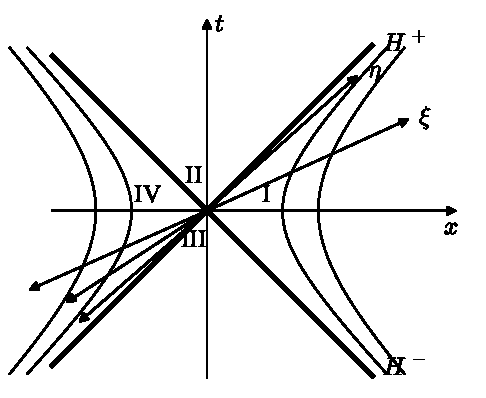
\includegraphics[width=0.72\textwidth]{fig_9.1.pdf}
\caption*{图 9.1\quad Rindler 坐标下的 Minkowski 时空。区域 I 是沿 $+x$ 方向做恒定加速的观者所能到达的区域。坐标 $(\eta,\xi)$ 可用于区域 I，也可单独用于区域 IV，但此时它们指向相反的方向。矢量场 $\partial_{\eta}$ 对应于洛伦兹推动（boost）对称性的生成元。视界 $H^{\pm}$ 是该矢量场的 Killing 视界，同时也是 Rindler 观者所见过去与未来的边界。}
\end{figure}

新坐标的取值范围为

\begin{equation*}
-\infty < \eta,\, \xi < +\infty,
\tag{9.132}
\end{equation*}

并且覆盖楔形区域 $x>|t|$，即图 9.1 中标记为区域 I 的部分。在这些坐标中，恒定加速路径 (9.126) 表为

\begin{align*}
\eta(\tau) &= \frac{\alpha}{a}\tau \\
\xi(\tau) &= \frac{1}{a}\ln\left(\frac{a}{\alpha}\right),
\tag{9.133}
\end{align*}

于是固有时正比于 $\eta$，而空间坐标 $\xi$ 为常数。特别地，$\alpha=a$ 的观者沿如下路径运动：

\begin{equation*}
\eta = \tau, \qquad \xi = 0.
\tag{9.134}
\end{equation*}

在这些坐标中度规取如下形式：

\begin{equation*}
ds^2 = e^{2a\xi}(-d\eta^2 + d\xi^2).
\tag{9.135}
\end{equation*}

带着这个度规，区域 I 被称为\textbf{Rindler 空间}（Rindler space），尽管它显然只是 Minkowski 空间的一部分。\textbf{Rindler 观者}（Rindler observer）就是沿恒定加速路径运动的观者，如 (9.133) 那样。Rindler 空间的因果结构酷似图 5.12 中 Schwarzschild 解最大延拓的 $r>2GM$ 区域。特别地，图 9.1 中标记为 $H^{+}$ 的类光直线 $x=t$，对于区域 I 中任何 $\eta=$ 常数的类空超曲面而言都是未来 Cauchy 视界；类似地，$H^{-}$ 是过去 Cauchy 视界。这些视界让人想起 Kruskal 图中的事件视界：Schwarzschild 中的静态观者（$r=$ 常数）正对应于 Rindler 空间中的恒定加速路径。

(9.135) 中的度规分量与 $\eta$ 无关，所以我们立刻知道 $\partial_{\eta}$ 是一个 Killing 矢量。但当然，这本来就是 Minkowski 时空，所以我们自以为了解所有 Killing 矢量是什么。确实，如果把 $\partial_{\eta}$ 用 $(t,x)$ 坐标表出，我们发现

\begin{align*}
\partial_{\eta} &= \frac{\partial t}{\partial\eta}\partial_t + \frac{\partial x}{\partial\eta}\partial_x \\
&= e^{a\xi}\left[\cosh(a\eta)\partial_t + \sinh(a\eta)\partial_x\right] \\
&= a(x\partial_t + t\partial_x).
\tag{9.136}
\end{align*}

这不多不少，正是与沿 $x$ 方向的推动（boost）相联系的那个 Killing 场。从这个表达式可以清楚地看到，这个 Killing 场自然地延拓到整个时空；在区域 II 和 III 中它是类空的，而在区域 IV 中它是类时的但指向过去。我们上面辨认出的那些视界，实际上就是 $\partial_{\eta}$ 的 Killing 视界。红移因子（在式 (6.12) 中定义为 Killing 矢量范数的大小）为

\begin{equation*}
V = e^{a\xi}.
\tag{9.137}
\end{equation*}

这个 Killing 视界的表面引力 $\kappa=\sqrt{\nabla_{\mu}V\nabla^{\mu}V}$ 于是为

\begin{equation*}
\kappa = a.
\tag{9.138}
\end{equation*}

这里并没有什么真实的引力，因为我们身处平直空间；但这个表面引力刻画了 Rindler 观者的加速度。

我们还可以把 (9.131) 中的符号翻转，在区域 IV 中定义坐标 $(\eta,\xi)$：

\begin{equation*}
t = -\frac{1}{a}e^{a\xi}\sinh(a\eta), \qquad x = -\frac{1}{a}e^{a\xi}\cosh(a\eta) \qquad (x < |t|).
\tag{9.139}
\end{equation*}

这个符号保证了在区域 IV 中 $\partial_{\eta}$ 与 $\partial_t$ 指向相反的方向。严格说来，我们不能在区域 I 和区域 IV 中同时使用 $(\eta,\xi)$，因为这两个坐标在各自区域中的取值范围相同；不过只要我们明确指明所谈论的是哪个区域，就不会出问题。之所以宁愿把同一套坐标标签用两次，而不是干脆引入新坐标，是因为度规 (9.135) 对区域 I 和区域 IV 都适用。

在曲面 $t=0$ 上，$\partial_{\eta}$ 是一个超曲面正交的类时 Killing 矢量，唯一的例外是它为零的那一点 $x=0$。因此这个矢量可用来定义一组正频与负频模式，并在此基础上为标量场的希尔伯特空间搭建 Fock 基。Rindler 坐标下无质量 Klein--Gordon 方程的形式为

\begin{equation*}
\Box\phi = e^{-2a\xi}\left(-\partial_{\eta}^{2} + \partial_{\xi}^{2}\right)\phi = 0.
\tag{9.140}
\end{equation*}

归一化的平面波 $g_k = (4\pi\omega)^{-1/2}e^{-i\omega\eta+ik\xi}$（其中 $\omega=|k|$）求解这个方程，而且显然具有正频，即 $\partial_{\eta}g_k=-i\omega g_k$。但我们需要的模式要相对于一个指向未来的 Killing 矢量具有正频，而在区域 IV 中扮演这一角色的是 $\partial_{(-\eta)}=-\partial_{\eta}$ 而非 $\partial_{\eta}$。为了对付这个麻烦，我们引入两组模式，一组支撑在区域 I 中，另一组支撑在区域 IV 中：

\begin{equation*}
\begin{aligned}
g_{k}^{(1)} &= \begin{cases} \dfrac{1}{\sqrt{4\pi\omega}}\, e^{-i\omega\eta+ik\xi} & \mathrm{I} \\[10pt] 0 & \mathrm{IV} \end{cases} \\[14pt]
g_{k}^{(2)} &= \begin{cases} 0 & \mathrm{I} \\[10pt] \dfrac{1}{\sqrt{4\pi\omega}}\, e^{+i\omega\eta+ik\xi} & \mathrm{IV} \end{cases}
\end{aligned}
\tag{9.141}
\end{equation*}

两种情形下都取 $\omega=|k|$；在两维中，空间波矢就是单独一个数 $k$。每一组模式都相对于相应的指向未来的类时 Killing 矢量具有正频：

\begin{gather*}
\partial_{\eta}\, g_{k}^{(1)} = -i\omega g_{k}^{(1)} \\
\partial_{(-\eta)}\, g_{k}^{(2)} = -i\omega g_{k}^{(2)}, \qquad \omega > 0.
\tag{9.142}
\end{gather*}

这两组模式连同它们的共轭，构成了对整个时空中波动方程任何解都完备的一组基模式。（单独一点 $x=t=0$ 是测度为零的集合，用不着为此担心。）在 Rindler 图的区域 II 和 III 中，这两组模式都不为零；把它们写成坐标 $\eta$ 和 $\xi$ 的形式时这一点被掩盖了，但这些函数可以解析延拓到未来和过去的区域。把相应的湮灭算符记作 $\hat{b}_{k}^{(1,2)}$，我们可以写出

\begin{equation*}
\phi = \int dk\left(\hat{b}_{k}^{(1)}g_{k}^{(1)} + \hat{b}_{k}^{(1)\dagger}g_{k}^{(1)*} + \hat{b}_{k}^{(2)}g_{k}^{(2)} + \hat{b}_{k}^{(2)\dagger}g_{k}^{(2)*}\right).
\tag{9.143}
\end{equation*}

这一展开是 (9.66) 式——用原始 Minkowski 模式所作的展开——的另一种选择；在两维中该式取如下形式：

\begin{equation*}
\phi = \int dk\left(\hat{a}_{k}f_{k} + \hat{a}_{k}^{\dagger}f_{k}^{*}\right).
\tag{9.144}
\end{equation*}

容易直接检验，模式 (9.141) 相对于内积 (9.94) 是恰当归一化的。在度规 (9.135) 中，曲面 $\eta=0$ 的指向未来的单位法矢量归一化为

\begin{equation*}
-1 = g_{\mu\nu}n^{\mu}n^{\nu} = -e^{2a\xi}(n^{0})^{2},
\tag{9.145}
\end{equation*}

即

\begin{equation*}
n^{0} = e^{-a\xi}.
\tag{9.146}
\end{equation*}

与此同时，空间度规的行列式满足

\begin{equation*}
\sqrt{\gamma} = e^{a\xi}.
\tag{9.147}
\end{equation*}

于是我们有 $n^{0}\sqrt{\gamma}=1$，而 Rindler 模式内积的计算与普通 Minkowski 模式的计算如出一辙。最终得到

\begin{align*}
(g_{k_1}^{(1)}, g_{k_2}^{(1)}) &= \delta(k_1 - k_2) \\
(g_{k_1}^{(2)}, g_{k_2}^{(2)}) &= \delta(k_1 - k_2) \\
(g_{k_1}^{(1)}, g_{k_2}^{(2)}) &= 0,
\tag{9.148}
\end{align*}

共轭模式也有类似结果。

这样就有两组模式——Minkowski 模式与 Rindler 模式——都可以用来展开平直两维时空中 Klein--Gordon 方程的解。虽然理论的希尔伯特空间在两种表示下是同一个，但它作为 Fock 空间的诠释却会不同；特别地，真空态会不相同。Minkowski 真空 $|0_{\mathrm{M}}\rangle$ 满足

\begin{equation*}
\hat{a}_{k}|0_{\mathrm{M}}\rangle = 0,
\tag{9.149}
\end{equation*}

在 Rindler 表示中它将被描述为一个多粒子态；同样，Rindler 真空 $|0_{\mathrm{R}}\rangle$ 满足

\begin{equation*}
\hat{b}_{k}^{(1)}|0_{\mathrm{R}}\rangle = \hat{b}_{k}^{(2)}|0_{\mathrm{R}}\rangle = 0,
\tag{9.150}
\end{equation*}

在 Minkowski 表示中它将被描述为一个多粒子态。在实际层面上，这种差异源于：单个 Rindler 模式永远无法写成正频 Minkowski 模式之和；在 $t=0$ 处 Rindler 模式只有支撑在半直线上的部分，而这样的函数不可能展开成纯粹正频的平面波。因此，用来定义 $|0_{\mathrm{R}}\rangle$ 的那些 Rindler 湮灭算符必然是 Minkowski 产生算符与湮灭算符的叠加，所以两个真空不可能重合。

Rindler 观者相对于推动 Killing 矢量 $\partial_{\eta}$ 的轨道是静止的。因此区域 I 中的这种观者将用 Rindler 模式 $g_{k}^{(1)}$ 来描述粒子：特别地，他会观测到 Rindler 真空中的态不含粒子，态 $\hat{b}_{k}^{(1)\dagger}|0_{\mathrm{R}}\rangle$ 含有一个频率为 $\omega=|k|$ 的粒子，如此等等。反过来，一位穿过 Minkowski 真空态的 Rindler 观者将探测到一个粒子背景，尽管惯性观者会把这个态描述成完全空无一物。Rindler 观者会探测到什么样的粒子呢？我们知道怎样回答这个问题：计算联系 Minkowski 模式与 Rindler 模式的 Bogoliubov 系数，再用它们确定 Rindler 粒子数算符在 Minkowski 真空中的期望值。这直截了当却十分繁琐，所以我们将走一条由 Unruh 提出的捷径。我们将找到一组模式，它与 Minkowski 模式共享同一个真空态（尽管对激发态的描述可能不同），但它与 Rindler 模式的交叠更为直接。做法是：从 Rindler 模式出发，把它们解析延拓到整个时空，再把这一延拓用原始的 Rindler 模式表出。

为了看清这是如何运作的，注意由 (9.131) 和 (9.139) 可知，在区域 I 和 IV 中，Minkowski 坐标 $(t,x)$ 与 Rindler 坐标 $(\eta,\xi)$ 之间有如下关系：

\begin{equation*}
\begin{aligned}
e^{-a(\eta-\xi)} &= \begin{cases} a(-t+x) & \mathrm{I} \\ a(t-x) & \mathrm{IV} \end{cases} \\[10pt]
e^{a(\eta+\xi)} &= \begin{cases} a(t+x) & \mathrm{I} \\ a(-t-x) & \mathrm{IV} \end{cases}
\end{aligned}
\tag{9.151}
\end{equation*}

因此，对于 $k>0$（从而 $\omega=k$）的模式 $g_{k}^{(1)}$，其在区域 I 中用 Minkowski 坐标表出的时空依赖为

\begin{align*}
\sqrt{4\pi\omega}\, g_{k}^{(1)} &= e^{-i\omega\eta+ik\xi} \\
&= e^{-i\omega(\eta-\xi)} \\
&= a^{i\omega/a}(-t+x)^{i\omega/a}.
\tag{9.152}
\end{align*}

这个函数在整个时空中的解析延拓很直截了当：对任何 $(t,x)$ 值都用这最后一个表达式即可。但我们希望处处都用原始的 Rindler 模式来表示结果；由于 $g_{k}^{(1)}$ 模式在区域 IV 中为零，我们需要让 $g_{k}^{(2)}$ 模式登场。在区域 IV 中用 Minkowski 坐标表出这些模式，对 $k>0$ 得到

\begin{align*}
\sqrt{4\pi\omega}\, g_{k}^{(2)} &= e^{+i\omega\eta+ik\xi} \\
&= e^{+i\omega(\eta+\xi)} \\
&= a^{-i\omega/a}(-t-x)^{-i\omega/a}.
\tag{9.153}
\end{align*}

这与我们想要的 (9.152) 的行为并不匹配。但若取复共轭并反转波数，就得到

\begin{align*}
\sqrt{4\pi\omega}\, g_{-k}^{(2)*} &= e^{-i\omega\eta+ik\xi} \\
&= e^{-i\omega(\eta-\xi)} \\
&= a^{i\omega/a}(t-x)^{i\omega/a} \\
&= a^{i\omega/a}[e^{-i\pi}(-t+x)]^{i\omega/a} \\
&= a^{i\omega/a}e^{\pi\omega/a}(-t+x)^{i\omega/a}.
\tag{9.154}
\end{align*}

组合

\begin{equation*}
\sqrt{4\pi\omega}\left(g_{k}^{(1)} + e^{-\pi\omega/a}g_{-k}^{(2)*}\right) = a^{i\omega/a}(-t+x)^{i\omega/a}
\tag{9.155}
\end{equation*}

因此沿整个曲面 $t=0$ 都有良好定义。我们明确考察了 $k>0$ 的情形，但对 $k<0$ 会得到完全相同的结果。

这个模式的恰当归一化版本由下式给出：

\begin{equation*}
h_{k}^{(1)} = \frac{1}{\sqrt{2\sinh\left(\frac{\pi\omega}{a}\right)}}\left(e^{\pi\omega/2a}g_{k}^{(1)} + e^{-\pi\omega/2a}g_{-k}^{(2)*}\right).
\tag{9.156}
\end{equation*}

这是 $g_{k}^{(1)}$ 模式的一个恰当的解析延拓；为了得到完备集，还需纳入 $g_{k}^{(2)}$ 模式的延拓，由类似的论证可知它为

\begin{equation*}
h_{k}^{(2)} = \frac{1}{\sqrt{2\sinh\left(\frac{\pi\omega}{a}\right)}}\left(e^{\pi\omega/2a}g_{k}^{(2)} + e^{-\pi\omega/2a}g_{-k}^{(1)*}\right).
\tag{9.157}
\end{equation*}

为了验证归一化——比如对 $h_{k}^{(1)}$——我们利用 (9.148)：

\begin{align*}
\left(h_{k_1}^{(1)}, h_{k_2}^{(1)}\right) &= \frac{1}{2\sqrt{\sinh\left(\frac{\pi\omega_1}{a}\right)\sinh\left(\frac{\pi\omega_2}{a}\right)}}\Bigg[e^{\pi(\omega_1+\omega_2)/2a}\left(g_{k_1}^{(1)}, g_{k_2}^{(1)}\right) \\
&\quad + e^{-\pi(\omega_1+\omega_2)/2a}\left(g_{-k_1}^{(2)*}, g_{-k_2}^{(2)*}\right)\Bigg] \\
&= \frac{1}{2\sqrt{\sinh\left(\frac{\pi\omega_1}{a}\right)\sinh\left(\frac{\pi\omega_2}{a}\right)}}\Bigg[e^{\pi(\omega_1+\omega_2)/2a}\,\delta(k_1 - k_2) \\
&\quad + e^{-\pi(\omega_1+\omega_2)/2a}\,\delta(-k_1 + k_2)\Bigg] \\
&= \frac{e^{\pi\omega_1/a} - e^{-\pi\omega_1/a}}{2\sinh\left(\frac{\pi\omega_1}{a}\right)}\,\delta(k_1 - k_2) \\
&= \delta(k_1 - k_2),
\tag{9.158}
\end{align*}

正如我们所愿。

现在可以把场用这些模式展开：

\begin{equation*}
\phi = \int dk\left(\hat{c}_{k}^{(1)}h_{k}^{(1)} + \hat{c}_{k}^{(1)\dagger}h_{k}^{(1)*} + \hat{c}_{k}^{(2)}h_{k}^{(2)} + \hat{c}_{k}^{(2)\dagger}h_{k}^{(2)*}\right).
\tag{9.159}
\end{equation*}

根据 9.4 节中关于 Bogoliubov 变换的讨论我们知道，用 $g_{k}^{(1,2)}$ 模式表出 $h_{k}^{(1,2)}$ 模式的表达式 (9.156) 与 (9.157)，蕴含着用算符 $\hat{c}_{k}^{(1,2)}$ 表出 Rindler 算符 $\hat{b}_{k}^{(1,2)}$ 的相应表达式：

\begin{align*}
\hat{b}_{k}^{(1)} &= \frac{1}{\sqrt{2\sinh\left(\frac{\pi\omega}{a}\right)}}\left(e^{\pi\omega/2a}\hat{c}_{k}^{(1)} + e^{-\pi\omega/2a}\hat{c}_{-k}^{(2)\dagger}\right) \\
\hat{b}_{k}^{(2)} &= \frac{1}{\sqrt{2\sinh\left(\frac{\pi\omega}{a}\right)}}\left(e^{\pi\omega/2a}\hat{c}_{k}^{(2)} + e^{-\pi\omega/2a}\hat{c}_{-k}^{(1)\dagger}\right).
\tag{9.160}
\end{align*}

于是我们可以把区域 I 中的 Rindler 粒子数算符

\begin{equation*}
\hat{n}_{\mathrm{R}}^{(1)}(k) = \hat{b}_{k}^{(1)\dagger}\hat{b}_{k}^{(1)},
\tag{9.161}
\end{equation*}

用新的算符 $\hat{c}_{k}^{(1,2)}$ 表示。

原先 $k>0$ 的正频 Minkowski 平面波模式 $f_k\propto e^{-i\omega(t-x)}$，只要 $\mathrm{Im}(t-x)\leq 0$，对复的 $(t,x)$ 都是解析且有界的。（这类模式称为“右行”（right-moving），因为它们描述向右传播的波。）只要我们把虚幂函数的支割线取在上半复 $(t-x)$ 平面内，我们的新模式 $h_{k}^{(1)}$ 也具有同样的性质——考察 (9.152) 和 (9.154) 即可看出；这与我们在 (9.154) 中取 $-1=e^{-i\pi}$ 的做法是一致的。类似的考虑也适用于 $h_{k}^{(2)}$ 模式，它们在下半复 $(t+x)$ 平面内解析且有界，正如 $k<0$ 的正频 Minkowski 平面波模式（左行）一样。因此，与原先的 Rindler 模式 $g_{k}^{(1,2)}$ 不同，我们知道 $h_{k}^{(1,2)}$ 模式能够纯粹用正频 Minkowski 模式 $f_k$ 表出。所以它们与 Minkowski 模式共享同一个真空态 $|0_{\mathrm{M}}\rangle$，于是

\begin{equation*}
\hat{c}_{k}^{(1)}|0_{\mathrm{M}}\rangle = \hat{c}_{k}^{(2)}|0_{\mathrm{M}}\rangle = 0.
\tag{9.162}
\end{equation*}

激发态将不会重合，但这不会困扰我们，因为我们关心的正是当态恰好处于 Minkowski 真空时 Rindler 观者会看到什么。例如，区域 I 中的观者将观测由算符 $\hat{b}_{k}^{(1)}$ 定义的粒子；频率为 $\omega$ 的这类粒子的期望数目由下式给出：

\begin{align*}
\langle 0_{\mathrm{M}}|\hat{n}_{\mathrm{R}}^{(1)}(k)|0_{\mathrm{M}}\rangle &= \langle 0_{\mathrm{M}}|\hat{b}_{k}^{(1)\dagger}\hat{b}_{k}^{(1)}|0_{\mathrm{M}}\rangle \\
&= \frac{1}{2\sinh\left(\frac{\pi\omega}{a}\right)}\langle 0_{\mathrm{M}}|e^{-\pi\omega/a}\hat{c}_{-k}^{(1)}\hat{c}_{-k}^{(1)\dagger}|0_{\mathrm{M}}\rangle \\
&= \frac{e^{-\pi\omega/a}}{2\sinh\left(\frac{\pi\omega}{a}\right)}\,\delta(0) \\
&= \frac{1}{e^{2\pi\omega/a} - 1}\,\delta(0),
\tag{9.163}
\end{align*}

其中我们用到了 $\hat{c}_{k}^{(1)\dagger}|0_{\mathrm{M}}\rangle$ 是归一化的单粒子态这一事实：

\begin{equation*}
\langle 0_{\mathrm{M}}|\hat{c}_{k}^{(1)}\hat{c}_{k}^{(1)\dagger}|0_{\mathrm{M}}\rangle = \delta(0).
\tag{9.164}
\end{equation*}

(9.163) 中的 $\delta$ 函数只是我们使用（不可平方可积的）平面波基模式带来的假象；如果我们构造的是归一化的波包，就会得到一个有限的结果，而谱完全相同。

结果 (9.163) 是一个温度为

\begin{equation*}
T = \frac{a}{2\pi}.
\tag{9.165}
\end{equation*}

的 Planck 谱。这样，\emph{以均匀加速度穿过 Minkowski 真空运动的观者会观测到粒子的热谱}。这就是\textbf{安鲁效应}。当然，热辐射不只是谱 (9.163) 而已；要真正称得上热，我们还应当检查在观测到的粒子之间没有隐匿的关联。这一点已经得到验证：Rindler 观者探测到的辐射是真正热的。在最基本的层面上，安鲁效应表明两批不同的观者（惯性的与 Rindler 的）会用极为不同的语言描述同一个态；在稍稍深入的层面上，它揭示了量子场论中真空本质上的热性质。

温度 $T=a/2\pi$ 是沿路径 $\xi=0$ 运动的观者会测得的温度，这条路径感受到的加速度为 $\alpha=a$。利用 (9.133) 可知，任何 $\xi=$ 常数的其他路径感受到的加速度为

\begin{equation*}
\alpha = ae^{-a\xi}
\tag{9.166}
\end{equation*}

因而应当测得温度为 $\alpha/2\pi$ 的热辐射。这与我们在第 6 章中关于沿某个 Killing 矢量 $K^{\mu}$ 的轨道运动的静态观者所见证的红移的讨论相一致；我们当时发现，在点 $x_1$ 处以频率 $\omega_1$ 发出的辐射，将在点 $x_2$ 处被观测到具有频率

\begin{equation*}
\omega_2 = \frac{V_1}{V_2}\omega_1,
\tag{9.167}
\end{equation*}

其中红移因子 $V$ 是 Killing 矢量的范数。在 (9.137) 中我们发现与 $\partial_{\eta}$ 相联系的红移因子为 $V=e^{a\xi}$，于是

\begin{equation*}
\omega_2 = e^{a(\xi_1 - \xi_2)}\omega_1.
\tag{9.168}
\end{equation*}

因此，如果 $\xi_1=0$ 处的观者探测到温度 $T=a/2\pi$，那么 $\xi_2=\xi$ 处的观者将看到它红移为温度 $T=ae^{-a\xi}/2\pi$，正如式 (9.166) 那样。特别地，当 $\xi\to+\infty$ 时温度一路红移到零。这是有道理的：无穷远处的 Rindler 观者近乎惯性观者，会对真空和粒子给出与普通 Minkowski 观者相同的定义。

安鲁效应告诉我们，加速观者会在 Minkowski 真空态中探测到粒子。当然，惯性观者会把同一个态描述成完全空无一物；实际上，能动张量的期望值会是 $\langle T_{\mu\nu}\rangle=0$。可是如果没有能量-动量，Rindler 观者们怎么能探测到粒子呢？这是一个微妙的问题，但绝不是矛盾。Rindler 观者要探测背景粒子，就必须携带一台探测器——某种与被探测粒子相耦合的装置。但如果探测器被维持在恒定加速度下，能量就不守恒；我们需要持续对探测器做功才能让它一直加速。从 Minkowski 观者的角度看，Rindler 探测器\emph{发射}粒子，也同样吸收粒子；一旦引入耦合，发射的可能性就不可避免。当探测器记录到一个粒子时，惯性观者会说它发射了一个粒子，并因此感受到一个辐射反作用力。归根结底，激发 Rindler 探测器所需的能量并非来自背景能动张量，而是来自我们为维持探测器加速而注入的能量。

\section{霍金效应与黑洞蒸发}

尽管发生在平直时空，安鲁效应却给了我们弯曲时空量子场论最重要的一课：“真空”和“粒子”是依赖于观者的概念，而非基本概念。实际上，鉴于我们对安鲁效应的理解，几乎可以立刻看出霍金效应是如何产生的。这不应太令人惊讶，因为我们已经指出过 Rindler 空间的因果结构与描述永恒黑洞的最大延拓 Schwarzschild 时空的因果结构之间的相似性。因此，我们将能够论证霍金辐射的存在，而无需在弯曲时空中做任何显式计算；当然，还有许多你可能想更深入考察的特征，那就需要充分动用弯曲度规的力量。除 Birrell 和 Davies (1982) 与 Wald (1994) 之外，还有一些很好的综述文章，你可以在其中找到对这里讨论的问题更全面的讨论。\footnote{T.A. Jacobson, “Introductory Lectures on Black Hole Thermodynamics,” Lectures at University of Utrecht (1996), http://www.fys.ruu.nl/\textasciitilde{}wwwthe/lectures/itfuu-0196.ps; R.M. Wald, “The thermodynamics of black holes,” \emph{Living Rev.\ Rel.} \textbf{4}, 6 (2001), http://arxiv.org/gr-qc/9912119; J. Traschen, “An introduction to black hole evaporation” (2000), http://arxiv.org/gr-qc/0010055.} 我们对霍金辐射的推导沿循 Jacobson 的做法。

考虑一个位于 Schwarzschild 黑洞之外、半径 $r_{1} > 2GM$ 处的静态观者。这样的观者沿着类时 Killing 矢量 $K = \partial_{t}$ 的轨道运动。在第 6 章中我们已经证明，对 Schwarzschild 时空中的静态观者，红移因子 $V = \sqrt{-K_{\mu}K^{\mu}}$ 由下式给出

\begin{equation*}
V = \sqrt{1 - \frac{2GM}{r}},
\tag{9.169}
\end{equation*}

相应的加速度大小则由下式给出：

\begin{equation*}
a = \frac{GM}{r\sqrt{r - 2GM}}.
\tag{9.170}
\end{equation*}

对于非常靠近事件视界的观者，$r_{1} - 2GM \ll 2GM$，这一加速度与 Schwarzschild 半径所标定的尺度相比会变得非常大，

\begin{equation*}
a_{1} \gg \frac{1}{2GM}.
\tag{9.171}
\end{equation*}

Schwarzschild 半径又标定了视界附近时空的曲率半径。因此，在由 $a_{1}^{-1} \ll 2GM$ 所设定的长度和时间尺度上观察，时空看上去基本上是平直的。让我们作一个至关重要的假设：在黑洞附近\emph{自由下落}的观者看来，某个标量场 $\phi$ 的量子态就像 Minkowski 真空（不含任何粒子）。这个假设是合理的，因为事件视界并不是一种局域的屏障；自由下落的观者在穿过视界时看不到任何异常发生。于是，这位静态观者看起来就跟平直时空中的常加速度观者一模一样，将探测到温度为 $T_{1} = a_{1}/2\pi$ 的安鲁辐射。

现在考虑位于无限远处——或者至少位于与 $2GM$ 相比大得多的距离 $r_{2}$ 处——的静态观者。在这种情形下，无论如何都谈不上能在 $a_{2}^{-1} \gg 2GM$ 的时间尺度上忽略时空曲率，因此没有理由预期他们会看到温度为 $a_{2}/2\pi$ 的辐射，这里 $a_{2}$ 在 $r_{2}$ 处取值。但是在视界附近观测到的辐射会带着恰当的红移传播到无限远。我们可以套用上一节末尾用过的论证，来确定这样的观者应当会看到什么；他们应当探测到红移至如下温度的热辐射：

\begin{equation*}
T_{2} = \frac{V_{1}}{V_{2}} T_{1} = \frac{V_{1}}{V_{2}} \frac{a}{2\pi}.
\tag{9.172}
\end{equation*}

在无限远处 $V_{2} \to 1$，于是观测到的温度为

\begin{equation*}
T = \lim_{r_{1} \to 2GM} \frac{V_{1} a_{1}}{2\pi} = \frac{\kappa}{2\pi},
\tag{9.173}
\end{equation*}

其中 $\kappa = \lim(Va)$ 是表面引力；对 Schwarzschild 黑洞，$\kappa = 1/4GM$。与平直时空中的加速观者不同，Schwarzschild 时空中的静态 Killing 矢量在无限远处具有有限的模长，因此视界附近的辐射只红移到一个有限值，而不会一直红移到零。远离黑洞的观者因此会看到黑洞发出的热辐射流，其温度正比于黑洞的表面引力。这就是著名的\textbf{霍金效应}（Hawking effect），这种辐射本身则被称为霍金辐射。

这种对霍金效应的推导虽然取巧，却没有任何不诚实之处。特别是，与加速度的联系清楚地说明了为什么温度正比于黑洞的表面引力（这一结论对更一般的黑洞同样成立，而不只是 Schwarzschild 黑洞）。不过，我们需要对我们所作的那个假设有清醒的认识：视界附近的真空态在自由下落的观者看来是非奇异的。用术语来说，就是取重整化能动张量在视界处为有限，或者等价地，两点函数满足 Hadamard 条件 (9.123)。

通过考察最大延拓 Schwarzschild 几何中各种可能的真空态，这个假设的含义会变得更加清楚。这些态对于由引力坍缩形成的现实黑洞来说不一定具有物理上的相关性，但在这种理想化情形中出现的各种可能性，能给现实世界带来有益的教益。我们将只描述这些态，而不定量地刻画它们，也不推导它们的任何性质；更多细节可参见上文所引的文献。

在寻找真空态时，我们也许会先去寻找一个在整个时空中都正则的态［在 Hadamard 意义下，式 (9.123)］。对最大延拓的 Schwarzschild 时空，Hartle 和 Hawking 找到了这样一个态，我们称之为\textbf{Hartle--Hawking 真空}（Hartle--Hawking vacuum）；的确，这是唯一的既处处正则、又在代表无限远处时间平移的 Schwarzschild Killing 矢量 $\partial_{t}$ 作用下不变的真空态。特别是，回忆图 5.16 所示的 Schwarzschild 共形图，Hartle--Hawking 真空在 $r = 2GM$ 处的过去和未来事件视界 $H^{\pm}$ 上正则，在过去和未来类光无限远 $\mathscr{I}^{\pm}$ 上也正则。根据上文对静态观者的讨论，我们应当会预期 Hartle--Hawking 真空中有热辐射从黑洞发出，而事实证明确实如此。然而，对这个态的仔细考察揭示出，还有一份等量的热辐射流从过去类光无限远（$\mathscr{I}^{-}$）流向黑洞；换句话说，它描述的是一个与其环境处于热平衡的黑洞。我们并不会用它来模拟我们宇宙中现实的黑洞。另一种真空更类似于经由引力坍缩形成的黑洞的真空态，这就是\textbf{Unruh 真空}（Unruh vacuum），它在 $H^{+}$ 上非奇异（因此预言了出射的霍金辐射），但没有来自 $\mathscr{I}^{-}$ 的入射辐射。Unruh 真空在 Schwarzschild 的过去视界 $H^{-}$ 上是奇异的；如果我们只是把它当作现实黑洞的模型，这并不会困扰我们，因为如图 5.17 那样经历引力坍缩的时空不会有白洞，也没有任何过去视界。最后，我们也许会去寻找这样一种真空态：既没有粒子进入黑洞，也没有粒子逃往无限远；换句话说，$\mathscr{I}^{\pm}$ 上通量为零。确实存在这样一个态，称为\textbf{Boulware 真空}（Boulware vacuum）。这样一种态的存在，似乎与我们从安鲁效应出发对霍金效应所作的论证相冲突，但仔细的分析表明，Boulware 真空在 $H^{-}$ 和 $H^{+}$ 上都是奇异的。于是，认为真空在视界附近的自由下落观者看来是正则的这一假设，在这个态中被违反了。

因此，对永恒 Schwarzschild 度规中真空态的仔细考察，与我们基于安鲁效应的推理是一致的；在 $H^{+}$ 上正则的态预言了预期形式的霍金辐射。注意，事件视界的存在对这一论证至关重要；如果没有这样的视界，态必须在视界上正则的要求就没有任何约束力。以中子星为例：其半径可能接近 Schwarzschild 半径，但其时空没有任何视界。中子星不发出任何霍金辐射。理解这一点的一个途径是认识到，静态中子星度规具有一个处处类时的 Killing 矢量，可以用它来定义贯穿整个时空延伸、并且在无限远处与 Minkowski 模式相匹配的正频模式。这样得到的真空态实际上会类似于 Boulware 真空，在 $\mathscr{I}^{\pm}$ 上没有通量；而完整的 Boulware 真空在视界上奇异这一点，在中子星情形中不会困扰我们，因为那里根本不存在任何视界。

为了绝对确信我们为现实的黑洞正确选择了真空态，我们应当考虑在一个过去近乎 Minkowski 时空、未来为 Schwarzschild 时空的时空中发生的引力坍缩，如图 5.17 所示。如果真空在 $\mathscr{I}^{-}$ 上取标准的 Minkowski 形式，我们就可以追问这些模式如何穿过坍缩几何传播到 $\mathscr{I}^{+}$，这就定义了一个如式 (9.45) 中的 S 矩阵，用以确定渐近观者会看到什么。Hawking 最初发现黑洞辐射时所做的正是这件事；计算涉及一些烦琐的代数，但基本上是直截了当的，得到的温度与我们上面推导的相同。

当然，从完整的计算中我们能学到的不仅仅是黑体温度；我们会想问，比如说，当发射辐射的波长与 Schwarzschild 半径相当时会发生什么——在这种情形下我们的近似显然失效了。如果我们仔细研究任意种类的粒子从任何一种黑洞（也就是同时容许电荷和自旋）的发射，就会发现发射辐射的谱具有如下形式

\begin{equation*}
\langle \hat{n}_{\omega} \rangle = \frac{\Gamma(\omega)}{e^{2\pi(\omega - \mu)/\kappa} \pm 1}.
\tag{9.174}
\end{equation*}

这里的 $\kappa$ 当然就是表面引力。参数 $\mu$ 是一个化学势（chemical potential），刻画黑洞丢掉其守恒量子数的倾向；带电黑洞优先发射与黑洞电荷同号的粒子，而转动黑洞优先发射与黑洞角动量同号的粒子。因此，霍金辐射趋向于把黑洞带回 Schwarzschild 状态。$\Gamma(\omega)$ 是一个灰体因子（greybody factor），可以把它想象成波包被引力场反散射回黑洞而产生的。在高频极限下波长非常小，反散射可以忽略；在极低的频率下，波长变得大于 Schwarzschild 半径，反散射就变得重要起来。虽然灰体因子的解析表达式很难导出，但在频率很大和很小的极限情形下，标量场的灰体因子满足

\begin{align*}
\Gamma(\omega) &\to 1, \qquad \omega \gg \frac{1}{GM} \\
\Gamma(\omega) &\to \frac{A}{4\pi} \omega^{2}, \qquad \omega \ll \frac{1}{GM},
\tag{9.175}
\end{align*}

其中 $A$ 是黑洞的面积。

从经典广义相对论的观点来看，黑洞发出热辐射的发现当然是令人惊讶的，因为我们曾经强调过，从事件视界内部的点逃逸到无限远是不可能的。理解眼下情形的一种形象方式，是用 Feynman 图来思考真空涨落：涨落由不断地出现又消失的虚粒子/反粒子对来表示。这幅图像也很有帮助，例如有助于理解诸如 Lamb 位移（Lamb shift）这样的观测现象——原子光谱会受到光子与虚电子/正电子对相互作用的影响。通常情况下，这些粒子对总会湮灭，它们的效应只是间接的，通过与虚粒子相耦合的过程的重整化体现出来。然而，在存在事件视界时，虚粒子对中的一个成员偶尔会落入黑洞，而它的同伴则逃逸到无限远，如图 9.2 所描绘。在这幅图像中，我们观测为霍金辐射的正是这些逃逸的虚粒子。虚粒子对的总能量必须相加为零，但从无限远来看，落入的粒子可以带有负能量，因为渐近类时的 Killing 矢量在视界内部是类空的。这幅图像有些不正规，但它为正在发生的事情提供了一种有用的启发。

\begin{figure}[H]
\centering
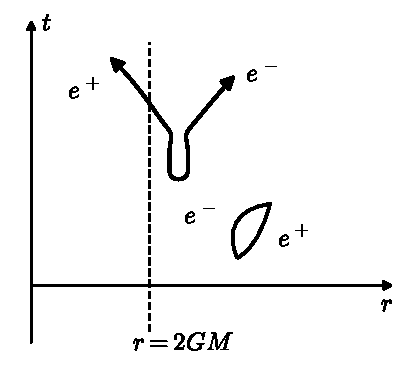
\includegraphics[width=0.72\textwidth]{fig_9.2.pdf}
\caption*{图 9.2\quad 真空涨落偶尔会导致粒子/反粒子对中的一个落入事件视界，而另一个则作为霍金辐射逃逸到无限远。}
\end{figure}

一旦知道了黑洞温度的公式，我们就能够确定黑洞参数与热力学变量之间各关系式中的比例常数，如式 (6.118) 所列。霍金辐射可以说最终圆满成就了黑洞力学与热力学的联姻；稳态黑洞的行为就如同能量 $E = M$、温度 $T = \kappa/2\pi$、熵 $S = A/4G$ 的热平衡物体。这确实是极其巨大的熵。对宇宙中的物质场而言，熵近似等于相对论性粒子的数目；在一个 Hubble 半径之内，这个数目算出来是

\begin{equation*}
S_{\mathrm{M}} \sim 10^{88}.
\tag{9.176}
\end{equation*}

另一方面，黑洞的熵是以 Planck 单位量度的视界面积（记住，我们从头到尾都在取 $\hbar = 1$）。我们可以换算成天体物理单位，得到

\begin{equation*}
S_{\mathrm{BH}} \sim 10^{90} \left( \frac{M}{10^{6} M_{\odot}} \right)^{2}.
\tag{9.177}
\end{equation*}

这样，单个百万太阳质量的黑洞（例如在我们自己银河系的中心以及许多其他星系的中心就能找到）所具有的熵，就比可见宇宙中全部物质的熵还要多。宇宙的总熵远比我们本来能把它做到的要小——只要把更多的质量投入黑洞就行。（当宇宙学家说熵 $S_{\mathrm{M}}$ 很大时，他们的意思是：在一个曲率半径之内竟然存在这么多熵，这很令人惊讶。）我们之所以处在这样一个低熵状态，其原因想必与初始条件有关，或许还与暴胀有关。

回到黑洞力学，我们看到一个难题：宏观黑洞的熵会非常巨大，但从统计力学的观点来看，熵本应量度可及态数目的对数。经典黑洞由少数几个参数（质量、电荷和自旋）确定，因此很难知道那些态可能是什么。尽管如此，我们可以采取这样的态度：这个矛盾其实无关紧要，因为关于黑洞状态的任何信息想必都藏在事件视界背后。

把量子力学包括进来，使这个难题变得更糟而非更好，因为黑洞不仅会辐射，而且会蒸发。当我们开始研究弯曲时空中的 QFT 时，我们定下的规则之一就是：假定背景度规固定不变，不去操心量子场自身的能动张量会产生什么影响。尽管如此，即使在量子力学中我们也有能量守恒（例如，表现为渐近平直时空中守恒的 ADM 质量）。因此，当霍金辐射逃逸到无限远时，我们可以放心地断定，它会把能量从黑洞带走，黑洞的质量必然因此缩减。（这个现象并不违反面积定理，因为量子场的能动张量在视界附近将不满足弱能量条件。）随着质量缩减，表面引力增大，温度也随之升高；这是一个失控的过程，全部质量会在有限的时间内蒸发殆尽。代入数值，可以得到量级如下的寿命

\begin{equation*}
\tau_{\mathrm{BH}} \sim \left( \frac{M}{m_{\mathrm{P}}} \right)^{3} t_{\mathrm{P}} \sim \left( \frac{M}{M_{\odot}} \right)^{3} \times 10^{71}\,\mathrm{sec},
\tag{9.178}
\end{equation*}

其中 $m_{\mathrm{P}} \sim 10^{-5}\,\mathrm{g}$ 是 Planck 质量，$t_{\mathrm{P}} \sim 10^{-43}\,\mathrm{sec}$ 是 Planck 时间。由于 Hubble 时间为 $H_{0}^{-1} \sim 10^{18}\,\mathrm{sec}$，一个太阳质量黑洞的寿命约为宇宙年龄的 $10^{53}$ 倍。这看起来是很长的时间，但我们在这里谈论的是原理性的问题。

你可以看出为什么黑洞熵的问题变得如此严峻：一旦黑洞蒸发殆尽，我们就不能再求助于事件视界来隐藏黑洞那些所谓的态。黑洞不复存在，只剩下它产生的霍金辐射。这种辐射被认为应当是严格热性的（出射粒子中没有隐藏的关联），这一事实意味着，它没有任何办法传递巨量的信息，而指定我们的熵计算所隐含的那些态正需要这些信息。这样一来，如果我们把两个非常不同的初始态分别坍缩成两个质量、电荷和自旋都相同的黑洞，它们就会辐射成两团不可分辨的霍金粒子云。系统在变成黑洞之前、为规定其状态而投入的信息，看来已被抹去；这就是\textbf{信息丢失佯谬}（information loss paradox）。量子场论和广义相对论都以幺正演化为特征——指定早期时刻的一个态所需的信息，与指定较晚时刻的一个态所需的信息严格相等，因为二者通过运动方程联系在一起。但在把 QFT 与 GR 结合的过程中，这种幺正性显然被破坏了。看来很可能我们在论证的某个地方作了某个不恰当的假设，但很难看出在哪里。

传达信息丢失佯谬实质的一个途径，是考察图 9.3 所示的设想中的蒸发黑洞共形图。我们并不真正知道完整的时空应当是什么样子，但这里我们作了似乎合理的假设：形成一个奇点，以及一个与之相伴随的事件视界，二者在黑洞完全蒸发后都消失，留下一个具有 Minkowski 型因果结构的时空。如果我们用 Cauchy 面来思考，问题就显而易见了。一张从类空无限远 $i^{0}$ 延伸到奇点过去侧某个 $r = 0$ 点的非编时面，其未来依赖域将是整个时空，因此这样的面会是一个 Cauchy 面。但是一张延伸到奇点未来侧某个 $r = 0$ 点的类似的面就不是 Cauchy 面了，因为事件视界背后的区域不在它的依赖域之中。因此，由于信息消失于奇点，过去无法由未来反推。换句话说，这个过程看起来是时间不可逆的（在微观意义上，而不仅仅是统计意义上），尽管用来预言它的动力学定律在时间反演下是完全不变的。

\begin{figure}[H]
\centering
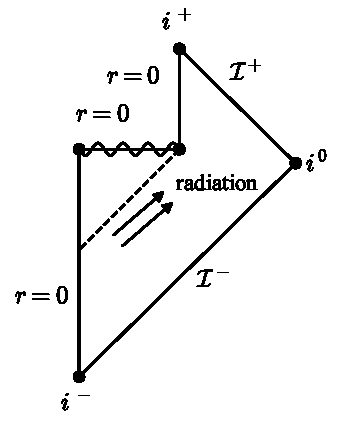
\includegraphics[width=0.72\textwidth]{fig_9.3.pdf}
\caption*{图 9.3\quad 设想中的蒸发黑洞共形图。能量被霍金辐射带走，黑洞最终完全蒸发殆尽，留下具有 Minkowski 时空因果结构的未来。落过事件视界进入奇点的信息看起来丢失了。}
\end{figure}

在讨论信息丢失佯谬时，请记住我们对黑洞蒸发的分析只是在量子场论与广义相对论相耦合的混合理论中进行的，并不是在现实的量子引力理论中。真实世界里究竟可能发生着什么呢？一种可能性是信息真的会丢失，幺正性真的会被破坏，而我们只得学会与之共处。许多物理学家觉得，引入这样一种可预见性的根本失效令人难以接受，而且也有论证表明，幺正性的破坏必然会导致能量守恒的破坏。另一种可能性是，幺正性在我们的世界中看似被破坏，只是因为进入黑洞的信息以某种方式逃逸到了空间一个不相连通的区域——一个婴儿宇宙（baby universe）。广义相对论预言黑洞中心存在奇点，而不是产生一个不相连通的区域；但显然我们正处于量子效应将剧烈改变经典预期的领域，所以我们应当保持开放的心态。

反对信息丢失的一些证据来自弦论。弦论自然地在 10 或 11 维时空中定义，其特征不仅在于一维的延展客体（弦），还在于统称为“膜”（branes）的各种更高维的延展客体。弦论的一个关键方面，是将玻色子与费米子联系起来的高度超对称性。在现实世界中，超对称性如果真的存在，就必须是自发破缺的，因为我们没有观测到与电子具有相同质量和电荷的玻色版本。但作为思想实验的工具，超对称性是无价的。人们可以构造出弦和膜的超对称位形，用来描述各种维度中的黑洞几何。弦论中有一个自由参数（实际上是一个标量场），即弦耦合（string coupling），它控制着引力的强度以及其他各种力的强度。如果我们考虑在某个弦耦合取值下描述黑洞的位形，那么当我们减小耦合时，Schwarzschild 半径最终会缩小到这个位形的尺寸以下，于是该位形就变成一团弱耦合的弦和膜。由于超对称性程度很高，我们可以确信，当我们改变弦耦合时，态的各种特征保持不变；特别是，我们预期自由度的数目（因而熵）不会改变。但在弱耦合区域没有黑洞，我们只有一团由通常自由度组成的“气体”（诚然，是高维中延展客体的气体），它的熵我们应该能够可靠地计算。

Strominger 和 Vafa 对一类特殊的五维超对称黑洞（带有不同种类的荷）考虑了这个过程。\footnote{A. Strominger and C. Vafa, “Microscopic origin of the Bekenstein-Hawking entropy,” \emph{Phys. Lett.} B \textbf{379}, 99 (1996), \texttt{http://arxiv.org/hep-th/9601029}。评述可参见 Johnson (2003)，或 A.W. Peet, “TASI lectures on black holes in string theory,” (2001), \texttt{http://arxiv.org/hep-th/0008241}。}他们得到了一个非凡的结果：系统在弱耦合下的自由度数目，与根据强耦合下的黑洞熵所预言的数目精确相符。由于黑洞熵非平庸地依赖于位形的荷，这种符合看来不大可能是偶然的。后续的研究把这一分析扩展到了其他类型的黑洞，并且不断地发现相符的结果。此外，通过考虑在弱耦合系统上的散射，我们甚至可以计算出预期的黑洞灰体因子；同样，结果与强耦合下的预期相符。因此，至少在弦论中，我们有极好的理由相信，黑洞辐射所隐含的自由度是真实存在的。

遗憾的是，弦论对态的计数，对于“黑洞状态的信息如何以某种方式传给出射的霍金辐射”这个问题，几乎没有提供直接的理解。尽管如此，我们当然应当认真对待事情果真如此的可能性，即使想象这样一个过程究竟如何实际运作还面临着严重的困难。当我们考虑把某些信息——或许以一套百科全书的形式——扔进一个大黑洞，而那时离黑洞蒸发殆尽还早得很的时候，困难就出现了。在这个阶段，黑洞温度很低，表面引力极小，事件视界附近的时空曲率也相当小。从百科全书的角度看，视界处没有任何特别的事情发生，我们应当预期它基本上毫发无损地落过视界。特别是，很难想象百科全书中的信息如何能够传递给早期发射出的霍金辐射。在幺正演化中，信息不可能被复制；它要么随百科全书一起落过视界，要么就必须在视界即将被穿越之前被有效地提取出来，而这似乎不合情理。我们或许可以指望，信息伴随着百科全书进入奇点附近的某个区域，并以某种方式保存在那里，直到黑洞变得很小的晚期。但到那时，大部分辐射粒子已经被发射出去了，最后一阵辐射所能到达的态的数目，一般会小于描述可能已经落入黑洞的各种不同态所需要的数目。

因此，要想认为信息以某种方式编码在出射辐射之中，看来就有必要在很早的时候就把关联编码到霍金粒子之中。我们刚刚论证过这一点很难做到，因为黑洞很大时，视界是一个平淡无奇的地方。摆脱这一困境的一个可以设想的办法，是迈出戏剧性的一步：放弃局域量子场论。换句话说，我们一直隐含地假设，信息可以被合理地描述为定域在空间的某个区域之中；这是通常量子场论的一个无可争议的特征。但量子引力也许有所不同，黑洞所包含的信息或许以某种方式非局域地弥散在视界之上。这个建议本身并不能直接给出把信息送进出射霍金辐射的机制，但它确实使我们给出的、关于为什么这样做会很困难的一些论证受到质疑。

非局域性的一种具体实现，以\textbf{全息原理}（holographic principle）为名。这个思想最初由 't Hooft 和 Susskind 提出：空间一个区域中的自由度数目，不是与该区域的体积成正比（正如在局域场论中所预期的那样），而是与该区域边界的面积成正比。\footnote{评述可参见 R. Bousso, “The Holographic Principle” (2002), \texttt{http://arxiv.org/hep-th/0203101}。}其灵感当然来自黑洞熵，后者按事件视界的面积标度；如果熵计数的是可及态的数目，全息就能解释为什么起作用的是面积，而不是所包围的体积。你也许会担心如何处理闭合宇宙的情形：在其中某个区域可能几乎由整个空间构成，边界却非常小；不过，只要把空间区域换成一组从边界向内延伸的“光片”（lightsheets），就可以表述出一个更具协变性的全息原理版本。全息原理最伟大的胜利是在第 8 章提到过的 AdS/CFT 对应中。在那里，反 de Sitter 背景上的量子引力物理，等价于定义在 AdS 边界上、维数低一维的无引力共形场论。可以设想，我们在宇宙中观测到的所有物理现象，都可以由某个定义在更低维数中的普通非引力理论的非局域全息投影来描述；我们究竟应当如何构造这样一种对应、又如何将它与观测联系起来，目前还完全不清楚，但宇宙学以及宇宙大尺度结构的考虑也许会是一个有希望的切入点。

关于黑洞熵、弦论和全息原理的这些评论，显然无意作为对一个非常活跃的研究领域的细致导引。毋宁说，它们意在指出引力物理前沿正在探索的若干可能性。经典广义相对论是迄今发明的最优美的物理理论，但我们完全有权利期待，GR 与物理学其他领域的综合，将揭示出我们如今只能想象的层层之美。


\appendix
 % 本文件由 scripts/assemble.py 自动装配，勿手改（改 parts/ 后重跑）
% 附录 A-J

% 附录A Maps between Manifolds
% 注：书页 428（p443）为空白页，附录 B 自书页 429（p444）始。

\chapter{流形之间的映射}

我们在第 2 章讨论流形时，曾经引入两个不同流形之间的映射，以及映射如何复合。这里我们将远为细致地考察这类映射，重点关注如何利用它们把张量场从一个流形携带到另一个流形。所讨论的流形，最终可能是一个子流形（submanifold）与它所嵌入的更大空间，也可能只是同一个抽象流形的两份不同副本彼此映射。

考虑两个流形 $M$ 和 $N$，维数可以不同，分别配有坐标系 $x^{\mu}$ 和 $y^{\alpha}$。设想我们有一个映射 $\phi : M \to N$，以及一个函数 $f : N \to \mathbf{R}$。显然，我们可以把 $\phi$ 与 $f$ 复合，构造出映射 $(f\circ\phi) : M \to \mathbf{R}$，它不过是 $M$ 上的一个函数。这种构造非常有用，足以让它拥有自己的名字；我们把 $f$ 被 $\phi$ 的\textbf{拉回}（pullback）记作 $\phi^{*}f$，定义为
\begin{equation*}
\phi^{*}f = (f\circ\phi).
\tag{A.1}
\end{equation*}
这个名字很有道理：我们把 $\phi^{*}$ 设想成把函数 $f$ 从 $N$ “拉回”到 $M$（见图 A.1）。

\begin{figure}[H]
\centering
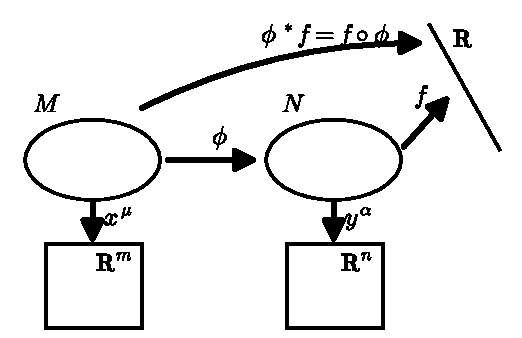
\includegraphics[width=0.72\textwidth]{fig_A.1.pdf}
\caption*{图 A.1\quad 映射 $\phi : M \to N$ 把函数 $f$ 从 $N$ 拉回到 $M$，所得无非是 $\phi$ 与 $f$ 的复合。}
\end{figure}

我们可以把函数拉回，却不能把函数推前。如果我们有一个函数 $g : M \to \mathbf{R}$，就没有办法把 $g$ 与 $\phi$ 复合而创造出 $N$ 上的函数——箭头无法正确地衔接起来。但是回想一下，矢量可以看成一种把光滑函数映为实数的导数算符。这使我们能够定义矢量的\textbf{推前}（pushforward）；若 $V(p)$ 是 $M$ 上点 $p$ 处的一个矢量，我们就通过给出它对 $N$ 上函数的作用，来定义 $N$ 上点 $\phi(p)$ 处的推前矢量 $\phi_{*}V$：
\begin{equation*}
(\phi_{*}V)(f) = V(\phi^{*}f).
\tag{A.2}
\end{equation*}
于是，要推前一个矢量场，我们可以说：“$\phi_{*}V$ 对任何函数的作用，无非就是 $V$ 对该函数之拉回的作用。”\footnote{遗憾的是，星号所在的位置并没有完全统一的标准；有些文献用上标 $*$ 表示推前、用下标 $*$ 表示拉回，所以要当心。}

这番讨论有点抽象，若能有一个更具体的描述就好了。我们知道，$M$ 上矢量的一个基由偏导数集合 $\partial_{\mu} = \partial/\partial x^{\mu}$ 给出，而 $N$ 上的基由偏导数集合 $\partial_{\alpha} = \partial/\partial y^{\alpha}$ 给出。因此，我们希望把 $V = V^{\mu}\partial_{\mu}$ 的分量与 $(\phi_{*}V) = (\phi_{*}V)^{\alpha}\partial_{\alpha}$ 的分量联系起来。把推前后的矢量作用到一个检验函数（test function）上，并利用链式法则 (2.12)，就能找到想要的关系：
\begin{align*}
(\phi_{*}V)^{\alpha}\partial_{\alpha}f &= V^{\mu}\partial_{\mu}(\phi^{*}f)\\
 &= V^{\mu}\partial_{\mu}(f\circ\phi)\\
 &= V^{\mu}\frac{\partial y^{\alpha}}{\partial x^{\mu}}\partial_{\alpha}f.
\tag{A.3}
\end{align*}
这个简单的公式让人难以抗拒地把推前操作 $\phi_{*}$ 看成一个矩阵算符 $(\phi_{*}V)^{\alpha} = (\phi_{*})^{\alpha}{}_{\mu}V^{\mu}$，其矩阵为
\begin{equation*}
(\phi_{*})^{\alpha}{}_{\mu} = \frac{\partial y^{\alpha}}{\partial x^{\mu}}.
\tag{A.4}
\end{equation*}
矢量在推前之下的这种行为，与坐标变换下矢量的变换定律有着不容误认的相似之处。事实上它是后者的推广，因为当 $M$ 与 $N$ 是同一个流形时，两种构造（正如我们将要讨论的）完全同一；但不要被迷惑，因为一般而言 $\mu$ 和 $\alpha$ 允许的取值并不相同，而且矩阵 $\partial y^{\alpha}/\partial x^{\mu}$ 也没有理由必须可逆。

让自己确信下面这件事是一次很有收获的练习：虽然给定映射 $\phi : M \to N$，你可以把矢量从 $M$ 推前到 $N$，但一般情况下你却不能把它们拉回——只管不断尝试去发明某种合适的构造，直到这种尝试的徒劳变得一目了然。由于 1-形式（one-form）与矢量对偶，听到 1-形式可以被拉回（但一般不能被推前）时，你不应感到惊讶。为了做到这一点，请记住 1-形式是从矢量到实数的线性映射。于是，$N$ 上 1-形式 $\omega$ 的拉回 $\phi^{*}\omega$ 可以通过它对一个 $M$ 上的矢量 $V$ 的作用来定义：让它等同于 $\omega$ 本身作用在 $V$ 的推前上：
\begin{equation*}
(\phi^{*}\omega)(V) = \omega(\phi_{*}V).
\tag{A.5}
\end{equation*}
再一次，形式上的拉回算符有一个简单的矩阵描述 $(\phi^{*}\omega)_{\mu} = (\phi^{*})_{\mu}{}^{\alpha}\omega_{\alpha}$，我们可以用链式法则把它推导出来。它由下式给出：
\begin{equation*}
(\phi^{*})_{\mu}{}^{\alpha} = \frac{\partial y^{\alpha}}{\partial x^{\mu}}.
\tag{A.6}
\end{equation*}
也就是说，它与推前式 (A.4) 中的矩阵是同一个，只不过当这个矩阵去拉回 1-形式时，缩并的当然是不同的指标。

有一种思考方式可以解释为什么拉回和推前只对某些对象有效、对另一些则不然，或许会有所帮助。如果我们把 $M$ 上光滑函数的集合记为 $\mathcal{F}(M)$，那么 $M$ 上点 $p$ 处的矢量 $V(p)$（也就是切空间 $T_{p}M$ 的一个元素）可以看成从 $\mathcal{F}(M)$ 到 $\mathbf{R}$ 的一个算符。但我们已经知道，函数上的拉回算符把 $\mathcal{F}(N)$ 映到 $\mathcal{F}(M)$，正如 $\phi$ 本身把 $M$ 映到 $N$，只是方向相反。因此，作用在矢量上的推前 $\phi_{*}$ 可以简单地通过映射的复合来定义，正如我们最初定义函数的拉回那样；如图 A.2 所示。类似地，若 $T_{q}N$ 是 $N$ 上点 $q$ 处的切空间，那么 $q$ 处的 1-形式 $\omega$（也就是余切空间 $T_{q}^{*}N$ 的一个元素）可以看成从 $T_{q}N$ 到 $\mathbf{R}$ 的一个算符。由于推前 $\phi_{*}$ 把 $T_{p}M$ 映到 $T_{\phi(p)}N$，1-形式的拉回 $\phi^{*}$ 同样可以看成单纯的映射复合，如图 A.3 所示。如果这种看法对你没有帮助，不必在意。但务必分清哪些东西存在、哪些不存在；概念本身很简单，引人误入歧途的只是忘掉了哪个映射朝哪个方向走。

你还会记得，$(0,l)$ 张量——即有 $l$ 个下指标而没有上指标的张量——是从 $l$ 个矢量的直积到 $\mathbf{R}$ 的线性映射。因此，我们不仅能拉回 1-形式，还能拉回具有任意数目下指标的张量。定义无非就是让原来的张量作用在推前后的矢量上：
\begin{equation*}
(\phi^{*}T)(V^{(1)},V^{(2)},\ldots,V^{(l)}) = T(\phi_{*}V^{(1)},\phi_{*}V^{(2)},\ldots,\phi_{*}V^{(l)}),
\tag{A.7}
\end{equation*}

\begin{figure}[H]
\centering
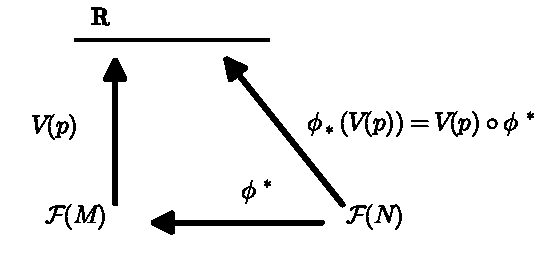
\includegraphics[width=0.72\textwidth]{fig_A.2.pdf}
\caption*{图 A.2\quad 矢量的推前，看成 $N$ 与 $M$ 上函数空间之间的一个映射，与从 $M$ 上的函数到 $\mathbf{R}$ 的一个映射的复合。}
\end{figure}

\begin{figure}[H]
\centering
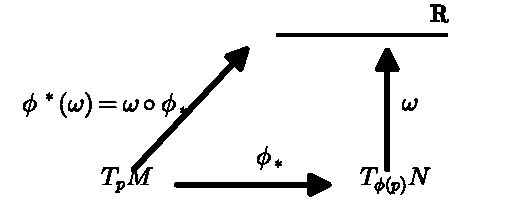
\includegraphics[width=0.72\textwidth]{fig_A.3.pdf}
\caption*{图 A.3\quad 1-形式的拉回，看成切空间 $T_{p}M$ 与 $T_{\phi(p)}N$ 之间的一个映射，与从 $T_{\phi(p)}N$ 到 $\mathbf{R}$ 的一个映射的复合。}
\end{figure}

其中 $T_{\alpha_{1}\cdots\alpha_{l}}$ 是 $N$ 上的一个 $(0,l)$ 张量。类似地，我们可以推前任意 $(k,0)$ 张量 $S^{\mu_{1}\cdots\mu_{k}}$，只要让它作用在拉回后的 1-形式上：
\begin{equation*}
(\phi_{*}S)(\omega^{(1)},\omega^{(2)},\ldots,\omega^{(k)}) = S(\phi^{*}\omega^{(1)},\phi^{*}\omega^{(2)},\ldots,\phi^{*}\omega^{(k)}).
\tag{A.8}
\end{equation*}
幸运的是，推前式 (A.4) 与拉回式 (A.6) 的矩阵表示可以推广到更高阶的张量，只需给每个指标指派一个矩阵即可；于是，对于 $(0,l)$ 张量的拉回，我们有
\begin{equation*}
\boxed{\,(\phi^{*}T)_{\mu_{1}\cdots\mu_{l}} = \frac{\partial y^{\alpha_{1}}}{\partial x^{\mu_{1}}}\cdots\frac{\partial y^{\alpha_{l}}}{\partial x^{\mu_{l}}}\,T_{\alpha_{1}\cdots\alpha_{l}},\,}
\tag{A.9}
\end{equation*}
而对于 $(k,0)$ 张量的推前，则有
\begin{equation*}
\boxed{\,(\phi_{*}S)^{\alpha_{1}\cdots\alpha_{k}} = \frac{\partial y^{\alpha_{1}}}{\partial x^{\mu_{1}}}\cdots\frac{\partial y^{\alpha_{k}}}{\partial x^{\mu_{k}}}\,S^{\mu_{1}\cdots\mu_{k}}.\,}
\tag{A.10}
\end{equation*}
于是，我们完整的图像如图 A.4 所示。注意，既有上指标又有下指标的张量，一般来说既不能被推前也不能被拉回。

\begin{figure}[H]
\centering
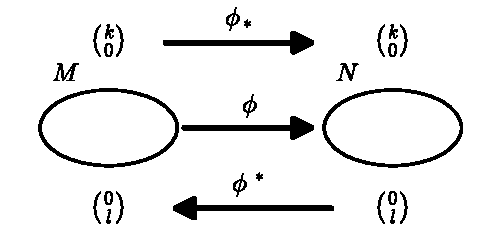
\includegraphics[width=0.72\textwidth]{fig_A.4.pdf}
\caption*{图 A.4\quad 映射 $\phi : M \to N$ 使我们能够拉回 $(0,l)$ 张量并推前 $(k,0)$ 张量。}
\end{figure}

一旦在一个简单的例子中看到这套机器运转起来，它就显得不那么令人生畏了。两个流形之间出现映射的一种常见情形，是 $M$ 实际上是 $N$ 的一个子流形，我们将在附录 C 中更仔细地讨论这种情形。基本想法是：存在一个从 $M$ 到 $N$ 的映射，它只是把 $M$ 的一个元素带到 $N$ 中“同一个”元素上。考虑嵌入 $\mathbf{R}^{3}$ 中的\emph{二维球面}（two-sphere），把它看成与原点相距单位距离的点的轨迹。如果在 $M = S^{2}$ 上取坐标 $x^{\mu} = (\theta,\phi)$，在 $N = \mathbf{R}^{3}$ 上取坐标 $y^{\alpha} = (x, y, z)$，那么映射 $\phi : M \to N$ 就由下式给出：
\begin{equation*}
\phi(\theta,\phi) = (\sin\theta\cos\phi,\ \sin\theta\sin\phi,\ \cos\theta).
\tag{A.11}
\end{equation*}
以这种方式把球面插进 $\mathbf{R}^{3}$，会在 $S^{2}$ 上诱导出一个度规，它正是平直空间度规的拉回。求出它的一个头脑简单的办法，是从 $\mathbf{R}^{3}$ 上的度规 $\mathrm{d}s^{2} = \mathrm{d}x^{2} + \mathrm{d}y^{2} + \mathrm{d}z^{2}$ 出发，把式 (A.11) 代入这个表达式，得到 $S^{2}$ 上的度规 $\mathrm{d}\theta^{2} + \sin^{2}\theta\,\mathrm{d}\phi^{2}$。让我们看看，用更体面的形式化方法，这个答案是如何得来的。（当然，如果我们在 $\mathbf{R}^{3}$ 上用球坐标来做，事情会更容易；但用费劲的办法做更有启发性。）偏导数矩阵由下式给出：
\begin{equation*}
\frac{\partial y^{\alpha}}{\partial x^{\mu}} =
\begin{pmatrix}
\cos\theta\cos\phi & \cos\theta\sin\phi & -\sin\theta\\
-\sin\theta\sin\phi & \sin\theta\cos\phi & 0
\end{pmatrix}.
\tag{A.12}
\end{equation*}
$S^{2}$ 上的度规只需把 $\mathbf{R}^{3}$ 的度规拉回就能得到，
\begin{align*}
(\phi^{*}g)_{\mu\nu} &= \frac{\partial y^{\alpha}}{\partial x^{\mu}}\frac{\partial y^{\beta}}{\partial x^{\nu}}\,g_{\alpha\beta}\\
 &= \begin{pmatrix} 1 & 0\\ 0 & \sin^{2}\theta \end{pmatrix},
\tag{A.13}
\end{align*}
这一点你可以轻易检验。所以，答案确实与朴素代入所得的相同，只不过现在我们知道了为什么。

% 附录B Diffeomorphisms and Lie Derivatives

\chapter{微分同胚与李导数}

% ---- 书页 429 / p444 ----
在本附录中，我们继续前一附录的探索，现在聚焦于两个流形其实是同一个流形这一特殊情形。到目前为止，我们一直谨慎地强调：映射 $\phi: M \to N$ 可以用来把某些东西拉回（式 (A.9)），并把另一些东西推前（式 (A.10)）。一般之所以不能两头都做，其原因可以追溯到 $\phi$ 可能不可逆。如果 $\phi$ 可逆（而且 $\phi$ 与 $\phi^{-1}$ 都是光滑的——我们总是隐含地如此假定），那么它就定义了 $M$ 与 $N$ 之间的一个微分同胚（diffeomorphism）。这只有在 $M$ 与 $N$ 实际上是同一个抽象流形时才可能成立；事实上，微分同胚的存在性正是“两个流形相同”的定义。微分同胚的美妙之处在于，我们既可以利用 $\phi$ 也可以利用 $\phi^{-1}$ 把张量从 $M$ 搬到 $N$；这将使我们能够定义任意张量的推前（pushforward）与拉回（pullback）。具体地说，对于 $M$ 上的一个 $(k,l)$ 型张量场 $T^{\mu_1\cdots\mu_k}{}_{\nu_1\cdots\nu_l}$，我们定义其推前为
\begin{equation*}
\begin{aligned}
(&\phi_* T)(\omega^{(1)}, \ldots, \omega^{(k)}, V^{(1)}, \ldots, V^{(l)}) \\
&= T(\phi^*\omega^{(1)}, \ldots, \phi^*\omega^{(k)}, [\phi^{-1}]_* V^{(1)}, \ldots, [\phi^{-1}]_* V^{(l)}),
\end{aligned}
\tag{B.1}
\end{equation*}
其中诸 $\omega^{(i)}$ 是 $N$ 上的 1-形式，诸 $V^{(i)}$ 是 $N$ 上的矢量。写成分量，这就变成
\begin{equation*}
(\phi_* T)^{\alpha_1\cdots\alpha_k}{}_{\beta_1\cdots\beta_l}
= \frac{\partial y^{\alpha_1}}{\partial x^{\mu_1}} \cdots \frac{\partial y^{\alpha_k}}{\partial x^{\mu_k}}
\frac{\partial x^{\nu_1}}{\partial y^{\beta_1}} \cdots \frac{\partial x^{\nu_l}}{\partial y^{\beta_l}}
T^{\mu_1\cdots\mu_k}{}_{\nu_1\cdots\nu_l}.
\tag{B.2}
\end{equation*}
逆矩阵 $\partial x^\nu/\partial y^\beta$ 的出现是合理的，因为 $\phi$ 可逆。注意，我们也可以按显而易见的方式定义拉回，但没有必要另写一套公式，因为拉回 $\phi^*$ 与经由逆映射的推前 $[\phi^{-1}]_*$ 是同一回事。

现在我们可以阐明微分同胚与坐标变换之间的关系了：它们是做同一件事的两种不同方式。如果你愿意这么说，微分同胚是“主动坐标变换”（active coordinate transformations），而传统的坐标变换则是“被动的”。考虑一个 $n$ 维流形 $M$，它带有坐标函数 $x^\mu : M \to \mathbf{R}^n$。要改变坐标，我们要么可以简单地引入新的函数 $y^\mu : M \to \mathbf{R}^n$（“保持流形不动，更换坐标映射”），要么也完全可以引入一个微分同胚 $\phi : M \to M$，此后坐标就成了拉回 $(\phi^* x)^\mu : M \to \mathbf{R}^n$（“移动流形上的点，然后求出这些新点的坐标”），如图 B.1 所示。在这个意义上，式 (B.2) 确实就是张量变换律，只不过是换了一个视角来看待它而已。

% ---- 书页 430 / p445 ----
由于微分同胚使我们能够对任意张量既作拉回又作推前，它提供了另一种比较流形上不同点处的张量的办法。给定一个微分同胚 $\phi : M \to M$ 和一个张量场 $T^{\mu_1\cdots\mu_k}{}_{\nu_1\cdots\nu_l}(x)$，我们可以构造张量在某点 $p$ 处的值与 $\phi^*[T^{\mu_1\cdots\mu_k}{}_{\nu_1\cdots\nu_l}(\phi(p))]$——即它在 $\phi(p)$ 处的值被拉回到 $p$——之间的差。这提示我们，可以定义另一种作用在张量场上的导数算符，用它来刻画张量在微分同胚的流动之下变化的快慢。然而，要做到这一点，单个离散的微分同胚是不够的；我们需要一个单参数族的微分同胚 $\phi_t$。这个族可以看成是一个光滑映射 $\mathbf{R} \times M \to M$，使得对每个 $t \in \mathbf{R}$ 我们都有一个微分同胚 $\phi_t$，并且满足 $\phi_s \circ \phi_t = \phi_{s+t}$。后面这个条件意味着 $\phi_0$ 是恒等映射。

单参数族的微分同胚可以看成是由矢量场产生的（反之亦然）。如果我们考察点 $p$ 在整个族 $\phi_t$ 之下的去向，显然它会描绘出 $M$ 中的一条曲线；由于 $M$ 上的每个点都是如此，这些曲线充满了流形（尽管在微分同胚具有不动点的地方可能会有退化）。我们可以把矢量场 $V^\mu(x)$ 定义为这些曲线中每一条在每一点处的切矢量组成的集合，取 $t = 0$ 时的值。$\mathbf{S}^2$ 上的一个例子由微分同胚 $\phi_t(\theta, \phi) = (\theta, \phi + t)$ 给出，如图 B.2 所示。我们可以把这一构造反过来，从任意一个矢量场出发定义一个单参数族的微分同胚。给定矢量场 $V^\mu(x)$，我们把该矢量场的\textbf{积分曲线}（integral curves）定义为求解下式的那些曲线 $x^\mu(t)$：
\begin{equation*}
\frac{d x^\mu}{d t} = V^\mu.
\tag{B.3}
\end{equation*}

\begin{figure}[H]
\centering
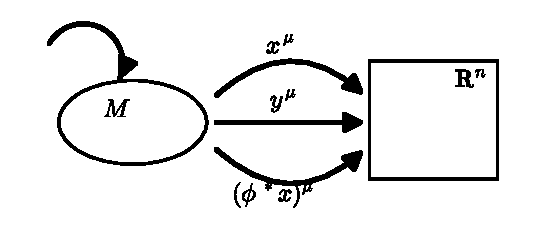
\includegraphics[width=0.72\textwidth]{fig_B.1.pdf}
\caption*{图 B.1\quad 由微分同胚 $\phi: M \to M$ 诱导的坐标变换。}
\end{figure}
\begin{figure}[H]
\centering
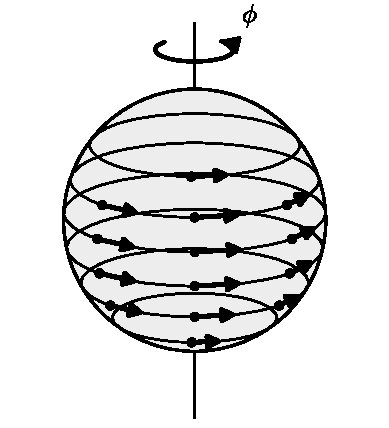
\includegraphics[width=0.72\textwidth]{fig_B.2.pdf}
\caption*{图 B.2\quad 二维球面上的一个微分同胚，由绕其轴的旋转给出。}
\end{figure}

% ---- 书页 431 / p446 ----
注意，这个看似眼熟的方程现在要按照与我们通常用法相反的意义来理解：我们给定的是矢量，由矢量来定义曲线。只要我们不干诸如撞上流形边缘之类的蠢事，式 (B.3) 的解保证存在；其证明归结为找到一个坐标系，使问题化为常微分方程的基本定理。我们的微分同胚 $\phi_t$ 表现的是“沿积分曲线流下去”，而与之相应的矢量场就称为该微分同胚的\textbf{生成元}（generator）。（令人混淆的是，矢量场及其积分曲线也会出现在类光超曲面的语境里，不过在那种场合被称为“生成元”（generators）的是曲线，而不是矢量场。）积分曲线在初等物理里无时无刻不在使用，只是没有被冠以这个名字。磁铁旁边铁屑描出的“磁感线”（lines of magnetic flux）不过是磁场矢量 $\mathbf{B}$ 的积分曲线罢了。

于是，给定矢量场 $V^\mu(x)$，我们就有了一个以 $t$ 为参数的微分同胚族，从而可以问：当我们沿积分曲线往下行进时，张量变化得有多快。对每个 $t$，我们可以把这个变化定义为张量被拉回到 $p$ 的值与它在 $p$ 处原有值之差，
\begin{equation*}
\Delta_t T^{\mu_1\cdots\mu_k}{}_{\nu_1\cdots\nu_l}(p)
= \phi_t^*\left[T^{\mu_1\cdots\mu_k}{}_{\nu_1\cdots\nu_l}(\phi_t(p))\right]
- T^{\mu_1\cdots\mu_k}{}_{\nu_1\cdots\nu_l}(p).
\tag{B.4}
\end{equation*}
注意，右端两项都是 $p$ 处的张量，如图 B.3 所示。于是我们把张量沿矢量场的\textbf{李导数}（Lie derivative）定义为
\begin{equation*}
\mathcal{L}_V T^{\mu_1\cdots\mu_k}{}_{\nu_1\cdots\nu_l}
= \lim_{t \to 0} \left( \frac{\Delta_t T^{\mu_1\cdots\mu_k}{}_{\nu_1\cdots\nu_l}}{t} \right).
\tag{B.5}
\end{equation*}
李导数是一个从 $(k,l)$ 型张量场到 $(k,l)$ 型张量场的映射，显然与坐标无关。由于这个定义实质上不过是把普通导数的传统定义用到张量的分量函数上，显然它是线性的，
\begin{equation*}
\mathcal{L}_V (a T + b S) = a \mathcal{L}_V T + b \mathcal{L}_V S,
\tag{B.6}
\end{equation*}

% ---- 书页 432 / p447 ----
\begin{figure}[H]
\centering
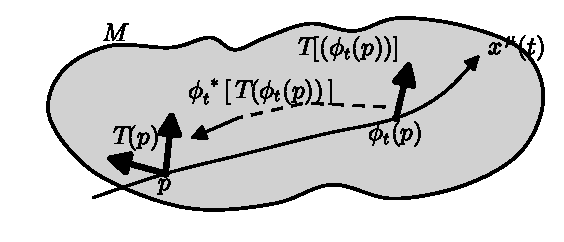
\includegraphics[width=0.72\textwidth]{fig_B.3.pdf}
\caption*{图 B.3\quad 张量沿矢量场积分曲线的变化速率，由如下方法算得：把点 $p$ 处原来的张量 $T(p)$ 与张量在点 $\phi_t(p)$ 处的值相比较——即把 $T(\phi_t(p))$ 拉回到 $p$。}
\end{figure}

并且服从 Leibniz 法则，
\begin{equation*}
\mathcal{L}_V (T \otimes S) = (\mathcal{L}_V T) \otimes S + T \otimes (\mathcal{L}_V S),
\tag{B.7}
\end{equation*}
其中 $S$ 和 $T$ 是张量，$a$ 和 $b$ 是常数。李导数实际上是比协变导数更原初的概念，因为它不需要指定联络（当然，它确实需要一个矢量场）。稍加思索你就会相信，作用在函数上时它就归结为普通的方向导数，
\begin{equation*}
\mathcal{L}_V f = V(f) = V^\mu \partial_\mu f.
\tag{B.8}
\end{equation*}

为了借助我们已知的其他运算来讨论李导数对张量的作用，选取一个适配于我们问题的坐标系是很方便的。具体地，我们将在坐标 $x^\mu = (x^1, \ldots, x^n)$ 中工作，其中 $x^1$ 是沿积分曲线的参数，其余坐标则随我们任意选取。于是矢量场取 $V = \partial/\partial x^1$ 的形式；也就是说，它的分量为 $V^\mu = (1, 0, 0, \ldots, 0)$。这个坐标系的魔力在于，参数为 $t$ 的微分同胚相当于一个从 $x^\mu$ 到 $y^\mu = (x^1 + t, x^2, \ldots, x^n)$ 的坐标变换。这样，由式 (A.6)，拉回矩阵简单地就是
\begin{equation*}
(\phi_t^*)_\mu{}^\nu = \delta_\mu{}^\nu,
\tag{B.9}
\end{equation*}
而从 $\phi_t(p)$ 拉回到 $p$ 的张量的分量就简单地是
\begin{equation*}
\phi_t^*\left[T^{\mu_1\cdots\mu_k}{}_{\nu_1\cdots\nu_l}(\phi_t(p))\right]
= T^{\mu_1\cdots\mu_k}{}_{\nu_1\cdots\nu_l}(x^1 + t, x^2, \ldots, x^n).
\tag{B.10}
\end{equation*}

% ---- 书页 433 / p448 ----
于是在这个坐标系中，李导数就成为
\begin{equation*}
\mathcal{L}_V T^{\mu_1\cdots\mu_k}{}_{\nu_1\cdots\nu_l}
= \frac{\partial}{\partial x^1} T^{\mu_1\cdots\mu_k}{}_{\nu_1\cdots\nu_l},
\tag{B.11}
\end{equation*}
特别地，矢量场 $U^\mu(x)$ 的导数是
\begin{equation*}
\mathcal{L}_V U^\mu = \frac{\partial U^\mu}{\partial x^1}.
\tag{B.12}
\end{equation*}
虽然这个表达式显然不是协变的，但我们知道对易子 $[V, U]$ 是一个良定义的张量，而且在这个坐标系中
\begin{align*}
[V, U]^\mu &= V^\nu \partial_\nu U^\mu - U^\nu \partial_\nu V^\mu \\
&= \frac{\partial U^\mu}{\partial x^1}. \tag{B.13}
\end{align*}
因此，$U$ 相对于 $V$ 的李导数在这个坐标系中的分量与 $V$ 和 $U$ 的对易子相同；但由于两者都是矢量，它们在任何坐标系中都必须相等：
\begin{equation*}
\mathcal{L}_V U^\mu = [V, U]^\mu.
\tag{B.14}
\end{equation*}
作为一个直接的推论，我们有 $\mathcal{L}_V U = -\mathcal{L}_U V$。正是因为式 (B.14)，对易子有时也被称为\textbf{李括号}（Lie bracket）。

为了导出 $\mathcal{L}_V$ 作用在 1-形式 $\omega_\mu$ 上的结果，我们先考虑它作用在标量 $\omega_\mu U^\mu$ 上的情形，这里 $U^\mu$ 是任意矢量场。首先利用这样一个事实：当作用在标量上时，对矢量场的李导数就归结为该矢量本身的作用：
\begin{align*}
\mathcal{L}_V (\omega_\mu U^\mu) &= V(\omega_\mu U^\mu) \\
&= V^\nu \partial_\nu (\omega_\mu U^\mu) \\
&= V^\nu (\partial_\nu \omega_\mu) U^\mu + V^\nu \omega_\mu (\partial_\nu U^\mu). \tag{B.15}
\end{align*}
然后对原来的标量使用 Leibniz 法则：
\begin{align*}
\mathcal{L}_V (\omega_\mu U^\mu) &= (\mathcal{L}_V \omega)_\mu U^\mu + \omega_\mu (\mathcal{L}_V U)^\mu \\
&= (\mathcal{L}_V \omega)_\mu U^\mu + \omega_\mu V^\nu \partial_\nu U^\mu - \omega_\mu U^\nu \partial_\nu V^\mu. \tag{B.16}
\end{align*}
令这两个表达式相等，并要求等式对任意 $U^\mu$ 都成立，我们就得到
\begin{equation*}
\mathcal{L}_V \omega_\mu = V^\nu \partial_\nu \omega_\mu + (\partial_\mu V^\nu) \omega_\nu,
\tag{B.17}
\end{equation*}
此式（正如对易子的定义那样）是完全协变的，尽管从表面上不容易看出来。

% ---- 书页 434 / p449 ----
用类似的步骤，我们可以定义任意张量场的李导数。答案可以写成
\begin{equation*}
\boxed{
\begin{aligned}
\mathcal{L}_V T^{\mu_1\mu_2\cdots\mu_k}{}_{\nu_1\nu_2\cdots\nu_l} ={}& V^\sigma \partial_\sigma T^{\mu_1\mu_2\cdots\mu_k}{}_{\nu_1\nu_2\cdots\nu_l} \\
&- (\partial_\lambda V^{\mu_1}) T^{\lambda\mu_2\cdots\mu_k}{}_{\nu_1\nu_2\cdots\nu_l} \\
&- (\partial_\lambda V^{\mu_2}) T^{\mu_1\lambda\cdots\mu_k}{}_{\nu_1\nu_2\cdots\nu_l} - \cdots \\
&+ (\partial_{\nu_1} V^\lambda) T^{\mu_1\mu_2\cdots\mu_k}{}_{\lambda\nu_2\cdots\nu_l} \\
&+ (\partial_{\nu_2} V^\lambda) T^{\mu_1\mu_2\cdots\mu_k}{}_{\nu_1\lambda\cdots\nu_l} + \cdots.
\end{aligned}
}
\tag{B.18}
\end{equation*}
尽管表面上看起来不是这样，这个表达式再一次是协变的。不过，倘若能有一个看上去明显是张量式的等价表达式，无疑会更让人安心。事实上我们可以写出
\begin{align*}
\mathcal{L}_V T^{\mu_1\mu_2\cdots\mu_k}{}_{\nu_1\nu_2\cdots\nu_l} ={}& V^\sigma \nabla_\sigma T^{\mu_1\mu_2\cdots\mu_k}{}_{\nu_1\nu_2\cdots\nu_l} \\
&- (\nabla_\lambda V^{\mu_1}) T^{\lambda\mu_2\cdots\mu_k}{}_{\nu_1\nu_2\cdots\nu_l} \\
&- (\nabla_\lambda V^{\mu_2}) T^{\mu_1\lambda\cdots\mu_k}{}_{\nu_1\nu_2\cdots\nu_l} - \cdots \\
&+ (\nabla_{\nu_1} V^\lambda) T^{\mu_1\mu_2\cdots\mu_k}{}_{\lambda\nu_2\cdots\nu_l} \\
&+ (\nabla_{\nu_2} V^\lambda) T^{\mu_1\mu_2\cdots\mu_k}{}_{\nu_1\lambda\cdots\nu_l} + \cdots, \tag{B.19}
\end{align*}
其中 $\nabla_\mu$ 代表\emph{任何}一个对称（无挠）的协变导数（当然也包括由度规导出的那些）。你可以验证，如果我们展开式 (B.19)，所有涉及联络系数的项都会相消，只剩下式 (B.18)。李导数公式的这两个版本在不同的场合各有用处。一个特别有用的公式是度规的李导数：
\begin{align*}
\mathcal{L}_V g_{\mu\nu} &= V^\sigma \nabla_\sigma g_{\mu\nu} + (\nabla_\mu V^\lambda) g_{\lambda\nu} + (\nabla_\nu V^\lambda) g_{\mu\lambda} \\
&= \nabla_\mu V_\nu + \nabla_\nu V_\mu, \tag{B.20}
\end{align*}
或者
\begin{equation*}
\boxed{\mathcal{L}_V g_{\mu\nu} = 2 \nabla_{(\mu} V_{\nu)},}
\tag{B.21}
\end{equation*}
其中 $\nabla_\mu$ 是由 $g_{\mu\nu}$ 导出的协变导数。

让我们把其中的某些想法放到广义相对论的语境中来。你会常常听到人们宣称，GR 是一个“微分同胚不变”的理论。这句话的意思是：如果宇宙由一个流形 $M$ 连同度规 $g_{\mu\nu}$ 和物质场 $\psi$ 来表示，而 $\phi : M \to M$ 是一个微分同胚，那么 $(M, g_{\mu\nu}, \psi)$ 与 $(M, \phi^* g_{\mu\nu}, \phi^* \psi)$ 这两组对象代表的是同一个物理情形。由于微分同胚不过是主动坐标变换，这其实是“该理论是坐标不变的”的一种高深说法。%
% ---- 书页 435 / p450 ----
这种说法虽然没错，却是极大的误解之源，原因很简单：它几乎没有传达任何信息。任何还算像样的物理理论都是坐标不变的，包括那些基于狭义相对论或 Newton 力学的理论；GR 在这方面并非独一无二。当人们说 GR 是微分同胚不变的时候，他们十有八九想的是两个（密切相关的）概念之一：这个理论不含“先验几何”（prior geometry），而且时空没有\emph{优先}的坐标系。其中第一点来源于这样的事实：度规是一个动力学变量，联络、体积元等等也随之而来。没有任何东西是事先提供给我们的，这与经典力学或 SR 不同。其后果是，我们无法靠死守某个适配于几何中某些绝对要素的特定坐标系来让日子好过一点。这种局面迫使我们格外小心；GR 中两个号称不同的位形（物质与度规的位形）有可能实际上是“相同的”——它们通过一个微分同胚彼此联系。在量子引力的路径积分方法中，我们希望对所有可能的位形求和，这时必须格外小心，不要让物理上无法区分的位形贡献不止一次，造成重复计数。而在 SR 或 Newton 力学中，一组优先坐标的存在把我们从这种含糊性中解救了出来。“GR 没有优先坐标系”这一事实常常被歪曲成这样的说法：它是坐标不变的（或“广义协变的”，或“微分同胚不变的”）；这两种说法都对，但其中一个比另一个更有内容。

另一方面，微分同胚不变性这一事实也可以好好地加以利用。回忆一下，引力与一组物质场 $\psi^i$ 耦合时的完整作用量，由 GR 的 Hilbert 作用量加上物质作用量之和给出，
\begin{equation*}
S = \frac{1}{16\pi G} S_H[g_{\mu\nu}] + S_M[g_{\mu\nu}, \psi^i].
\tag{B.22}
\end{equation*}
Hilbert 作用量 $S_H$ 单独拿出来看是微分同胚不变的，因此如果要整个作用量不变，物质作用量 $S_M$ 也必须如此。我们可以把微分同胚之下 $S_M$ 的变分写成
\begin{equation*}
\delta S_M = \int d^n x \, \frac{\delta S_M}{\delta g_{\mu\nu}} \delta g_{\mu\nu}
+ \int d^n x \, \frac{\delta S_M}{\delta \psi^i} \delta \psi^i.
\tag{B.23}
\end{equation*}
我们考虑的不是场的任意变分，而只是由微分同胚产生的那些变分。尽管如此，物质的运动方程告诉我们，$S_M$ 对 $\psi^i$ 的变分对任何变分都为零，因为作用量的引力部分不含物质场。于是，对一个微分同胚不变的理论而言，式 (B.23) 右端第一项也必须为零。如果微分同胚由一个无穷小矢量场 $V^\mu(x)$ 生成，度规的无穷小改变就简单地由它沿 $V^\mu$ 的李导数给出；由式 (B.20) 我们有

% ---- 书页 436 / p451 ----
\begin{align*}
\delta g_{\mu\nu} &= \mathcal{L}_V g_{\mu\nu} \\
&= 2 \nabla_{(\mu} V_{\nu)}. \tag{B.24}
\end{align*}
令 $\delta S_M = 0$ 便意味着
\begin{align*}
0 &= \int d^n x \, \frac{\delta S_M}{\delta g_{\mu\nu}} \nabla_\mu V_\nu \\
&= - \int d^n x \, \sqrt{-g} \, V_\nu \nabla_\mu \left( \frac{1}{\sqrt{-g}} \frac{\delta S_M}{\delta g_{\mu\nu}} \right), \tag{B.25}
\end{align*}
其中我们能够去掉 $\nabla_{(\mu} V_{\nu)}$ 的对称化，因为 $\delta S_M/\delta g_{\mu\nu}$ 本来就是对称的。要求式 (B.25) 对由任意矢量场 $V^\mu$ 生成的微分同胚都成立，并利用能动张量（energy-momentum tensor）的定义，即式 (4.75)，我们便恰好得到能量-动量守恒定律，
\begin{equation*}
\nabla_\mu T^{\mu\nu} = 0.
\tag{B.26}
\end{equation*}
$T_{\mu\nu}$ 的守恒是一个强有力的论断；我们竟然从微分同胚不变性这么弱的要求把它导了出来，这也许会让人吃惊。实际上我们偷偷夹带了一个强得多的假设，即“物质的”作用量与“引力的”作用量之间有一刀两断的分离（意思是没有物质场出现在引力作用量之中）。比方说，如果有一个标量场既乘在标量曲率上，又出现在物质作用量中（正如第 4 章讨论过的标量-张量理论那样），这个假设就被破坏了，$T_{\mu\nu}$ 自身也就不再守恒。

回忆一下，在第 3 章里我们谈到过对称性和 Killing 矢量，并一再提请读者参阅附录。现在我们对微分同胚已经有了更多的了解，理解对称性便是水到渠成的事了。如果张量经 $\phi$ 拉回之后保持不变，我们就说微分同胚 $\phi$ 是某个张量 $T$ 的一个\textbf{对称性}（symmetry）：
\begin{equation*}
\phi^* T = T.
\tag{B.27}
\end{equation*}
虽然对称性可以是分立的，但拥有一个单参数族的对称性 $\phi_t$ 也很常见。如果这个族由矢量场 $V^\mu(x)$ 生成，那么式 (B.27) 就相当于
\begin{equation*}
\mathcal{L}_V T = 0.
\tag{B.28}
\end{equation*}
由式 (B.12)，对称性的一个推论是：如果 $T$ 在某个单参数族的微分同胚下对称，我们总能找到一个坐标系，使得 $T$ 的全部分量都与其中一个坐标无关（即矢量场的积分曲线坐标）。%
% ---- 书页 437 / p452 ----
反之亦然：如果全部分量都与其中一个坐标无关，那么与该坐标相联系的偏导数矢量场就生成该张量的一个对称性。

最重要的对称性是度规的对称性，即 $\phi^* g_{\mu\nu} = g_{\mu\nu}$ 的情形。这种类型的微分同胚称为等距变换（isometry）。如果单参数族的等距变换由矢量场 $K^\mu(x)$ 生成，那么 $K^\mu$ 就是一个 Killing 矢量场。$K^\mu$ 为 Killing 矢量的条件于是就是
\begin{equation*}
\mathcal{L}_K g_{\mu\nu} = 0,
\tag{B.29}
\end{equation*}
或者由式 (B.20)，
\begin{equation*}
\nabla_{(\mu} K_{\nu)} = 0.
\tag{B.30}
\end{equation*}
我们认得出来，最后一个版本正是 Killing 方程，即式 (3.174)。从第 3 章的讨论我们知道，如果时空有一个 Killing 矢量，我们就能找到一个坐标系，使度规与其中一个坐标无关，并且量 $p_\mu K^\mu$ 沿具有切矢量 $p^\mu$ 的测地线保持常数。一旦我们建立起微分同胚与李导数的这套机制，Killing 矢量的推导就要优雅得多。

\section{习题}

% 习题编号照原书
\textbf{1.}\quad 在欧几里得三维空间中，求出并画出下列矢量场的积分曲线：
\begin{equation*}
A = \frac{y - x}{r} \frac{\partial}{\partial x} - \frac{x + y}{r} \frac{\partial}{\partial y}
\end{equation*}
和
\begin{equation*}
B = x y \frac{\partial}{\partial x} - y^2 \frac{\partial}{\partial y}.
\end{equation*}
计算 $C = \mathcal{L}_A B$，并画出 $C$ 的积分曲线。

% ---- 书页 438 / p453 ----
% （本页为空白页）

% 附录C Submanifolds

\chapter{子流形}

% ---- 书页 439 / p454 ----
子流形（submanifold）的概念——某个另一流形的子集，其维数可能（而且通常确实）更低——在直观上直截了当；然而，若了解到随之而来还有一套形式理论，也不必惊讶。子流形在广义相对论中无处不在——作为时空的边界、固定时刻的超曲面、更大的空间在对称性作用下被叶状分层而成的空间——因此值得我们花力气去理解它们究竟是如何运作的。

考虑一个 $n$ 维流形 $M$ 和一个 $m$ 维流形 $S$，其中 $m \leq n$，以及一个映射 $\phi : S \to M$。如果映射 $\phi$ 既是 $C^\infty$ 的又是单射（one-to-one），而且逆映射 $\phi^{-1} : \phi[S] \to S$ 也是 $C^\infty$ 的，那么我们就说像 $\phi[S]$ 是 $M$ 的一个\textbf{嵌入子流形}（embedded submanifold）。如果 $\phi$ 局部是单射但不必全局是单射（也就是说，$\phi[S]$ 在 $M$ 中可能有自交），那么我们就说 $\phi[S]$ 是 $M$ 的一个\textbf{浸入子流形}（immersed submanifold）。当我们不加任何限定语地说到“子流形”时，我们心目中想的是嵌入的情形。$n$ 维流形的一个 $m$ 维子流形被称为具有\textbf{余维数}（codimension）$n - m$。

如附录 A 所讨论的，映射 $\phi : S \to M$ 可以用来把 $(k,0)$ 型张量从 $S$ 推前到 $M$，并把 $(0,l)$ 型张量从 $M$ 拉回到 $S$。特别地，给定点 $q \in S$ 及其像 $\phi(q) \in M$，切空间 $T_{\phi(q)}\phi[S]$ 自然地被等同于 $n$ 维矢量空间 $T_{\phi(q)}M$ 的一个 $m$ 维子空间。如果你想一想把矢量定义为沿曲线的方向导数，这就完全讲得通了；任何曲线 $\gamma : \mathbf{R} \to S$ 显然通过复合在 $M$ 中定义了一条曲线（$\phi \circ \gamma : \mathbf{R} \to M$），后者又定义了一个方向导数。类似地，$M$ 上的微分形式也可以拉回到 $S$，办法是把它们的作用限制在子空间 $T_{\phi(q)}\phi[S]$ 中的矢量上。

定义子流形的另一种方式，是把它定义为一族函数取某组指定固定值的地方。$M$ 的一个 $m$ 维子流形可以用 $n - m$ 个函数 $f^a(x)$（其中 $a$ 从 1 取到 $n - m$）规定为使诸 $f^a$ 等于某些常数 $f^a_*$ 的那些点 $x$ 组成的集合：
\begin{gather*}
f^1(x) = f^1_* \\
f^2(x) = f^2_* \\[1em]
f^{n-m}(x) = f^{n-m}_*. \tag{C.1}
\end{gather*}

% ---- 书页 440 / p455 ----
这些函数应当是非退化的，这样子流形才真正具有维数 $m$。注意，以这种方式定义的子流形是 $M$ 的一个实实在在的子集；它与我们在前面定义中所说的 $\phi[S]$ 等价。为方便起见，从今往后我们会倾向于模糊原来的空间与其作为子流形的嵌入之间的区别，径直称之为“子流形 $S$”。

为了看清子流形这两种定义之间的关系，设想在 $\phi[S] \subset M$ 的一个邻域内构造一组坐标 $x^\mu = \{f^a, y^\alpha\}$，它由这 $n - m$ 个函数 $f^a$ 再加上另外 $m$ 个函数 $y^\alpha$ 组成。于是我们可以把函数 $y^\alpha$ 拉回来充当 $S$ 上的坐标，而映射 $\phi : S \to M$ 就简单地由下式给出：
\begin{equation*}
\phi : (y^\alpha) \to (f^a_*, y^\alpha).
\tag{C.2}
\end{equation*}
一个简单的例子是二维球面 $S^2$，事实上我们当初就是把它定义为 $\mathbf{R}^3$ 中到原点距离为单位长度的那些点的集合。在球坐标 $(r, \theta, \phi)$ 下，这等价于要求 $r = 1$，于是坐标 $r$ 就扮演了函数 $f(x)$ 的角色，而 $\theta$ 和 $\phi$ 则是 $S^2$ 上的诱导坐标（induced coordinates）。

我们在式 (B.3) 处已经提到，指定单个矢量场会导致一族积分曲线，它们正是一维子流形。我们可能会想到推广这一构造：用一组若干个矢量场来定义更高维的子流形。设想我们有一个 $n$ 维流形 $M$、一个 $m$ 维子流形 $S$，以及一组 $p$ 个线性无关的矢量场 $V^\mu_{(a)}$，其中 $p \geq m$。这些矢量场“拼合起来定义了 $S$”这一说法意味着每个矢量处处都与 $S$ 相切，从而诸 $V^\mu_{(a)}$ 张成每一个切空间 $T_pS$；我们说 $S$ 是这些矢量场的一个\textbf{积分子流形}（integral submanifold）。然而，任意给定的一组矢量场未必真的能拼合起来定义这样的子流形。它们能否做到，由 \textbf{Frobenius 定理}揭示：一组矢量场 $V^\mu_{(a)}$ 能拼合起来定义积分子流形，当且仅当它们的全部对易子都落在由诸 $V^\mu_{(a)}$ 张成的空间之中；也就是说，若
\begin{equation*}
[V_{(a)}, V_{(b)}]^\mu = \alpha^c V^\mu_{(c)}
\tag{C.3}
\end{equation*}
对某一组系数 $\alpha^c(x)$ 成立。（用群论的语言说，这意味着这些矢量场构成一个李代数（Lie algebra）。）我们不打算给出证明，但希望这个结果在数学上讲得通。如果这些矢量场要拼合起来构成一个子流形 $S$，它们必须处处保持与 $S$ 相切。但对易子 $[V, W]$ 等价于李导数 $\mathcal{L}_V W$，后者量度的正是当我们沿着 $V$ 行进时 $W$ 如何变化。如果这个李导数不留在由这些矢量所定义的空间之内，那就意味着 $W$ 开始伸出子流形 $S$ 之外。矢量场拼合起来构成子流形的例子很容易找；在第 5.2 节我们讨论过，与球对称性相联系的三个 Killing 矢量如何把一个三维空间叶状分层成二维球面。（注意，积分子流形的维数可以小于矢量场的数目。）关于 Frobenius 定理的讨论，可参见 Schutz (1980)。

% ---- 书页 441 / p456 ----
Frobenius 定理有一个有趣的替代表述，它使用微分形式。首先注意，任意一组 $p$ 个线性无关的 1-形式 $\omega_\mu^{(a)}$ 定义了 $T_pM$ 的一个 $(n-p)$ 维矢量子空间，称为这组形式的\textbf{零化子}（annihilator），它由 $T_pM$ 中满足
\begin{equation*}
\omega_\mu^{(a)} V^\mu = 0
\tag{C.4}
\end{equation*}
（对每一个 $\omega_\mu^{(a)}$ 都满足）的那些矢量 $V^\mu$ 组成。因此，我们可以不问一组矢量场是否拼合起来定义了一组子流形，而是问一组 1-形式 $\omega_\mu^{(a)}$ 所定义的一组矢量子空间是否拼合起来，充当一组子流形的切空间。为了理解何时会发生这种情形，回想式 (C.1) 中 $m$ 维子流形的定义：它是使一组 $p = n - m$ 个函数 $f^a(x)$ 被取为常数值的地方。常函数是其外微分为零（$(\mathrm{d}f^a)_\mu = \nabla_\mu f^a$ 为零）的函数；但如果一个函数只是沿某个子流形才为常数，那就意味着
\begin{equation*}
\mathrm{d}f^a(V) = V^\mu \nabla_\mu f^a = 0
\tag{C.5}
\end{equation*}
对所有与该子流形相切的矢量 $V^\mu \in T_pS$ 成立。反过来也对：如果一个矢量 $V^\mu$ 被所有梯度 $\nabla_\mu f^a$ 零化，它必然与相应的子流形 $S$ 相切。因此，如果一组 1-形式各自都是恰当的，$\omega_\mu^{(a)} = \nabla_\mu f^a$，那么它们所零化的矢量空间肯定定义子流形，即诸 $f^a$ 沿之为常数的那些子流形。但是，如果一组 $p$ 个 1-形式零化某个子空间，那么作为原来诸形式之线性组合的任何另一组 $p$ 个 1-形式也同样会零化它。因此我们说，一组 1-形式 $\omega_\mu^{(a)}$ 是\textbf{成面的}（surface-forming），如果其中每一个成员都能表示成一组恰当形式的线性组合；也就是说，如果存在函数 $g^a{}_b(x)$ 和 $f^a(x)$ 使得
\begin{equation*}
\omega_\mu^{(a)} = \sum_b g^a{}_b \nabla_\mu f^b.
\tag{C.6}
\end{equation*}
当然，手里拿到一组形式时，可能很难判断是否存在函数使这一条件得到满足；这正是 Frobenius 定理的对偶表述派上用场的地方。这一定理的版本断言：一组 1-形式 $\omega_\mu^{(a)}$ 是成面的，当且仅当零化子中的每一对矢量同时也被外微分 $\mathrm{d}\omega^{(a)}$ 所零化。换句话说，形式组 $\omega_\mu^{(a)}$ 将满足式 (C.6)，当且仅当对每一对满足 $\omega_\mu^{(a)} V^\mu = 0$ 与 $\omega_\mu^{(a)} W^\mu = 0$（对所有 $a$）的矢量 $V^\mu$ 和 $W^\mu$，我们还有
\begin{equation*}
\nabla_{[\mu} \omega_{\nu]}^{(a)} V^\mu W^\nu = 0.
\tag{C.7}
\end{equation*}

% ---- 书页 442 / p457 ----
满足这一条件的一组形式有时被称为“闭的”（closed），这显然是单个形式为闭（即其外微分为零）这一概念的推广。我们不去证明 Frobenius 定理的对偶表述与矢量场版本的等价性，但其中显然涉及把我们的这组形式作用在矢量场的对易子（C.3）上。

% ---- 书页 443 / p458 ----
% 附录D Hypersurfaces
\chapter{超曲面}

超曲面（hypersurface）是 $n$ 维流形 $M$ 的一个 $(n-1)$ 维（余维数为一）子流形 $\Sigma$。（当然，如果 $n = 3$，$\Sigma$ 本也完全可以就叫“曲面”，但为了统一起见，我们将继续使用“超”字。）超曲面在广义相对论中极为有用，随之而来的是大量的形式理论。在本附录中，我们汇集超曲面研究中的一批结果：法矢量、类光超曲面的生成元、超曲面的 Frobenius 定理、高斯法坐标、诱导度规、投影张量、外曲率，以及带边流形。这有点像一桌自助餐（smorgasbord），难免带着可想而知的一团杂乱，但希望它同样可口而富于营养。

规定超曲面 $\Sigma$ 的一种方式，是令单个函数等于一个常数，
\begin{equation*}
f(x) = f_*.
\tag{D.1}
\end{equation*}
矢量场
\begin{equation*}
\zeta^\mu = g^{\mu\nu} \nabla_\nu f
\tag{D.2}
\end{equation*}
将是该曲面的法矢量，其意义是它与 $T_p\Sigma \subset T_pM$ 中的所有矢量都正交。如果 $\zeta^\mu$ 是类时的，就称该超曲面是类空的；如果 $\zeta^\mu$ 是类空的，超曲面就是类时的；而如果 $\zeta^\mu$ 是类光的，超曲面也是类光的。任何与某个法矢量场成比例的矢量场，
\begin{equation*}
\xi^\mu = h(x) \nabla^\mu f
\tag{D.3}
\end{equation*}
（其中 $h(x)$ 是某个函数）本身就是法矢量场；由于法矢量在相差一个标度因子的意义下唯一，任何法矢量都可以写成这种形式。因此，对类时和类空超曲面，我们可以定义法矢量的归一化版本，
\begin{equation*}
n^\mu = \pm \frac{\zeta^\mu}{|\zeta_\mu \zeta^\mu|^{1/2}}.
\tag{D.4}
\end{equation*}
于是，对类空曲面有 $n^\mu n_\mu = -1$，对类时曲面有 $n^\mu n_\mu = +1$；除一个整体定向之外，这样的法矢量场是唯一的。对类空曲面，这个符号通常选得使 $n^\mu$ 指向未来（future-directed）。

类光超曲面有一个特殊性质：它们可以分解成一族类光测地线，称为该超曲面的\textbf{生成元}（generators）。让我们看看这是怎么回事。

% ---- 书页 444 / p459 ----
注意，法矢量 $\zeta^\mu$ 除了与 $\Sigma$ 正交之外，还与 $\Sigma$ 相切，因为类光矢量与自身正交。因此，满足
\begin{equation*}
\zeta^\mu = \frac{d x^\mu}{d\alpha},
\tag{D.5}
\end{equation*}
的积分曲线将是包含在超曲面之内的类光曲线。这些曲线 $x^\mu(\alpha)$ 必然是测地线，尽管 $\alpha$ 未必是仿射参量。为了验证这一论断，回想测地线方程的一般形式可以表示为
\begin{equation*}
\zeta^\mu \nabla_\mu \zeta_\nu = \eta(\alpha) \zeta_\nu,
\tag{D.6}
\end{equation*}
其中 $\eta(\alpha)$ 是一个函数，若 $\alpha$ 是仿射参量它将为零。我们直接代入式 (D.2) 并计算：
\begin{align*}
\zeta^\mu \nabla_\mu \zeta_\nu &= \zeta^\mu \nabla_\mu \nabla_\nu f \\
&= \zeta^\mu \nabla_\nu \nabla_\mu f \\
&= \zeta^\mu \nabla_\nu \zeta_\mu \\
&= \frac{1}{2} \nabla_\nu (\zeta^\mu \zeta_\mu).
\tag{D.7}
\end{align*}
在第二行中我们用到了无挠条件，即作用在标量上的协变导数是对易的。注意，尽管在 $\Sigma$ 本身上 $\zeta^\mu \zeta_\mu = 0$，我们不能确定 $\nabla_\nu (\zeta^\mu \zeta_\mu)$ 为零，因为在超曲面之外 $\zeta^\mu \zeta_\mu$ 可能非零。如果这个梯度为零，式 (D.7) 就是测地线方程，我们就证完了。但如果它不为零，我们可以用 $\zeta^\mu \zeta_\mu = 0$ 作为定义子流形 $\Sigma$ 的另一种方式，而它的导数就定义了一个法矢量。因此，必有
\begin{equation*}
\nabla_\mu (\zeta^\nu \zeta_\nu) = g \nabla_\mu f = g \zeta_\mu,
\tag{D.8}
\end{equation*}
其中 $g(x)$ 是某个标量函数。把它代入式 (D.7) 就得到
\begin{equation*}
\zeta^\mu \nabla_\mu \zeta_\nu = \frac{1}{2} g \zeta_\nu,
\tag{D.9}
\end{equation*}
它与测地线方程 (D.6) 等价。当然，一旦我们知道路径 $x^\mu(\alpha)$ 是测地线，就可以随意用仿射参量 $\lambda(\alpha)$ 对它重新参数化。等价地说，我们用一个标量函数 $h(x)$ 去缩放法矢量场，
\begin{equation*}
\xi^\mu = h \zeta^\mu,
\tag{D.10}
\end{equation*}
使得 $\xi^\mu \nabla_\mu \xi^\nu = 0$。惯例正是这么做的，并使用相应的切矢量
\begin{equation*}
\xi^\mu = \frac{d x^\mu}{d\lambda}
\tag{D.11}
\end{equation*}

% ---- 书页 445 / p460 ----
作为 $\Sigma$ 的法矢量。类光测地线 $x^\mu(\lambda)$ 的并集就是类光超曲面 $\Sigma$，它们便是 $\Sigma$ 的生成元。

由式 (D.3) 我们知道，与超曲面正交的矢量场可以写成 $\xi^\mu = h \nabla^\mu f$ 的形式。在第 4 章的习题中曾请你证明，这蕴含
\begin{equation*}
\xi_{[\mu} \nabla_\nu \xi_{\sigma]} = 0,
\tag{D.12}
\end{equation*}
或者用微分形式的记号，
\begin{equation*}
\xi \wedge \mathrm{d}\xi = 0.
\tag{D.13}
\end{equation*}
其逆命题——任何满足此方程的矢量场都与某个超曲面正交——从基本原理出发较难证明，但它是 Frobenius 定理对偶表述的直接推论。设想我们有两个矢量 $V^\mu$ 和 $W^\mu$，两者都被一个服从式 (D.12) 的 1-形式 $\xi_\mu$ 所零化。由 Frobenius 定理（式 (C.7)），$\xi_\mu$ 将定义一个超曲面，当且仅当
\begin{equation*}
\nabla_{[\mu} \xi_{\nu]} V^\mu W^\nu = 0.
\tag{D.14}
\end{equation*}
把式 (D.12) 中的表达式作用到 $V^\mu W^\nu$ 上，并展开反对称化括号，我们得到
\begin{align*}
\xi_{[\mu} \nabla_\nu \xi_{\sigma]} V^\mu W^\nu
&= \tfrac{1}{3} \left( \xi_\mu \nabla_{[\nu} \xi_{\sigma]} + \xi_\nu \nabla_{[\sigma} \xi_{\mu]} \right) V^\mu W^\nu + \tfrac{1}{3} \xi_\sigma \nabla_{[\mu} \xi_{\nu]} V^\mu W^\nu \\
&= \tfrac{1}{3} \xi_\sigma \nabla_{[\mu} \xi_{\nu]} V^\mu W^\nu,
\tag{D.15}
\end{align*}
其中在最后一行我们用到了 $V^\mu$ 和 $W^\mu$ 被 $\xi_\mu$ 零化这一事实。但由于 $\nabla_{[\mu} \xi_{\nu]} V^\mu W^\nu$ 是一个标量而 $\xi_\sigma$ 是一个非零的 1-形式，式 (D.15) 能为零的唯一办法就是式 (D.14) 成立。因此，式 (D.12) 为真当且仅当 $\xi_\mu$ 超曲面正交（hypersurface-orthogonal）。

在流形（或其一部分）上放置一个自然适配于某个超曲面 $\Sigma$ 的坐标系往往很方便；高斯法坐标（Gaussian normal coordinates）就提供了做到这一点的一种便捷办法。先在 $\Sigma$ 上选取坐标 $y^i = \{y^1, \ldots, y^{n-1}\}$。在每一点 $p \in \Sigma$ 处，构造以 $n^\mu$ 为在 $p$ 处切矢量的那条（唯一的）测地线。令 $z$ 为每条测地线上的仿射参量。[如果 $n^\mu$ 已归一化且 $z(p) = 0$，则这个参量是唯一的。]$\Sigma$ 邻域中的任何一点 $q$ 都位于某条这样的测地线上。对每个这样的点，我们指派坐标 $\{z, y^1, \ldots, y^{n-1}\}$，其中诸 $y^i$ 是由我们所构造的测地线连到 $q$ 的那个点 $p$ 的坐标。这些坐标 $\{z, y^1, \ldots, y^{n-1}\}$ 就称为\textbf{高斯法坐标}（Gaussian normal coordinates）（不要与“Riemann 法坐标”相混淆，后者是从单个点 $p$ 出发沿所有方向走测地线构造出来的）。如果我们走到测地线聚焦并相交的地方，这些坐标终将失去良好定义，但在包含 $\Sigma$ 的某个区域内它们总是存在的。关于高斯法坐标的所有陈述都应理解为在其良好定义的区域内适用。

% ---- 书页 446 / p461 ----
与坐标函数 $\{z, y^1, \ldots, y^{n-1}\}$ 相联系的是坐标基矢量场 $\{\partial_z, \partial_1, \ldots, \partial_{n-1}\}$。为记号方便，让我们把这些矢量场记作
\begin{gather*}
(\partial_z)^\mu = n^\mu, \\
(\partial_i)^\mu = Y^\mu_{(i)},
\tag{D.16}
\end{gather*}
其中第一行是有意义的，因为 $\partial_z$ 不过是原来的法矢量 $n^\mu$ 沿测地线的延拓。相对于这组基矢量，度规取一种简单的形式。首先，我们知道
\begin{equation*}
g_{zz} = ds^2 (\partial_z, \partial_z) = n_\mu n^\mu = \pm 1,
\tag{D.17}
\end{equation*}
因为 $n^\mu$ 正是从 $\Sigma$ 发出的那些测地线的归一化切矢量。为了把这一符号歧义打包起来，让我们把它记作 $\sigma$：
\begin{equation*}
\sigma = n_\mu n^\mu = \pm 1.
\tag{D.18}
\end{equation*}
但我们也有 $g_{zi} = n_\mu Y^\mu_{(i)} = 0$，这可以直接验证。从原来的曲面 $\Sigma$ 出发，在那里按假设有 $n_\mu Y^\mu_{(i)} = 0$（因为 $n^\mu$ 与 $\Sigma$ 正交）。然后我们计算
\begin{align*}
\frac{D}{dz} \left( n_\mu Y^\mu_{(i)} \right) &= n^\nu \nabla_\nu \left( n_\mu Y^\mu_{(i)} \right) \\
&= n^\nu n_\mu \nabla_\nu Y^\mu_{(i)} \\
&= Y^\nu_{(i)} n_\mu \nabla_\nu n^\mu \\
&= \frac{1}{2} Y^\nu_{(i)} \nabla_\nu \left( n_\mu n^\mu \right) \\
&= 0.
\tag{D.19}
\end{align*}
让我们逐行解释这个推导。第一行就是方向协变导数 $D/dz$ 的定义。第二行用了 Leibniz 法则，再加上 $n_\mu$ 沿测地线被平行移动这一事实（$n^\nu \nabla_\nu n_\mu = 0$）。第三行用了 $n^\mu$ 与 $Y^\nu_{(i)}$ 都是坐标基矢量、因而其李括号为零这一事实：$[n, Y_{(i)}]^\mu = n^\nu \nabla_\nu Y^\mu_{(i)} - Y^\nu_{(i)} \nabla_\nu n^\mu = 0$。第四行再次用了 Leibniz 法则和 $n_\mu$ 被平行移动的事实，而第五行则仅仅反映了 $n_\mu n^\mu = \sigma$ 为常数这一事实。

于是我们可以把高斯法坐标下的度规写成
\begin{equation*}
\boxed{\, ds^2 = \sigma \, \mathrm{d}z^2 + \gamma_{ij} \, \mathrm{d}y^i \mathrm{d}y^j, \,}
\tag{D.20}
\end{equation*}
其中 $\gamma_{ij} = g(\partial_i, \partial_j)$ 一般而言是所有坐标 $\{z, y^1, \ldots, y^{n-1}\}$ 的函数。我们没有对几何作任何假设；我们只是选取了一个使度规取特定形式的坐标系。

% ---- 书页 447 / p462 ----
注意，令 $z$ 等于常数定义了一族与原来曲面 $\Sigma$ 微分同胚的超曲面；式 (D.20) 中不出现非对角项 $g_{zi}$，这反映的正是矢量场 $n^\mu$ 与所有这些曲面都正交，而不只是与原来那一个正交这一事实。高斯法坐标绝不冷僻；我们时时刻刻都在使用它们。简单的例子有 Minkowski 空间中的惯性坐标，
\begin{equation*}
ds^2 = -\mathrm{d}t^2 + \mathrm{d}x^2 + \mathrm{d}y^2 + \mathrm{d}z^2,
\tag{D.21}
\end{equation*}
或者欧几里得三维空间中的球坐标，
\begin{equation*}
ds^2 = \mathrm{d}r^2 + r^2 \mathrm{d}\theta^2 + r^2 \sin^2 \theta \, \mathrm{d}\phi^2.
\tag{D.22}
\end{equation*}
宇宙学中通常的 Robertson--Walker 坐标则给出了一个稍不那么平凡的例子，
\begin{equation*}
ds^2 = -\mathrm{d}t^2 + a^2(t) \left[ \frac{\mathrm{d}r^2}{1 - \kappa r^2} + r^2 \mathrm{d}\Omega^2 \right].
\tag{D.23}
\end{equation*}
当然，RW 几何是高度对称的（均匀且各向同性）。但是，既然我们刚刚看到高斯法坐标总可以被定义，我们就知道，通过改动度规的空间分量，便可以描述完全一般的几何。这提供了一种流行的描述宇宙学微扰的方式；对平直空间切片，我们把“同步规范”（synchronous gauge）定义为
\begin{equation*}
ds^2 = -\mathrm{d}t^2 + a^2(t) (\delta_{ij} + h_{ij}) \mathrm{d}x^i \mathrm{d}x^j,
\tag{D.24}
\end{equation*}
其中 $h_{ij}(t, \mathbf{x})$ 是度规微扰。（推广到弯曲的空间切片是直截了当的。）再一次，我们没有对几何作任何假设，只是选了一个可能方便的坐标系。

回想把任意子流形嵌入的映射 $\phi : \Sigma \to M$ 使我们能够把度规从 $M$ 拉回到 $\Sigma$。给定 $\Sigma$ 上的坐标 $y^i$ 和 $M$ 上的坐标 $x^\mu$，我们把子流形上的\textbf{诱导度规}（induced metric）定义为
\begin{equation*}
(\phi^* g)_{ij} = \frac{\partial x^\mu}{\partial y^i} \frac{\partial x^\nu}{\partial y^j} g_{\mu\nu}.
\tag{D.25}
\end{equation*}
当子流形是一个超曲面时，这个诱导度规恰好就是在式 (D.20) 中出现的 $\gamma_{ij}$。为看清这一点，注意高斯法坐标是式 (C.2) 所描述的自然嵌入坐标的特例。我们有一个在 $M$ 上由 $z = z_*$ 定义的超曲面 $\Sigma$，在 $\Sigma$ 上定义了坐标 $y^i$，以及一个由下式给出的映射 $\phi : \Sigma \to M$：
\begin{equation*}
\phi : y^i \to x^\mu = (z_*, y^i).
\tag{D.26}
\end{equation*}
给定 $M$ 上度规的形式 (D.20)，立即可知在这个映射下拉回 (D.25) 就简单地是
\begin{equation*}
(\phi^* g)_{ij} = \gamma_{ij}.
\tag{D.27}
\end{equation*}

% ---- 书页 448 / p463 ----
请记住，这个方程只应在高斯法坐标中求值；否则右端连意义都没有。

与诱导度规一道，子流形还从它们所嵌入的流形那里继承一个诱导体积元。回想带有度规 $g_{\mu\nu}$ 的 $n$ 维流形上的体积元由 Levi-Civita 张量给出，后者可以表示为
\begin{equation*}
\epsilon = \sqrt{|g|} \, \mathrm{d}x^1 \wedge \cdots \wedge \mathrm{d}x^n.
\tag{D.28}
\end{equation*}
为了得到子流形 $\Sigma$ 上的体积元，方便的做法是引入高斯法坐标 $(z, y^1, \ldots, y^{n-1})$，在其中度规取式 (D.20) 的形式。于是 $\Sigma$ 上的体积元 $\widehat{\epsilon}$ 将取如下形式：
\begin{equation*}
\widehat{\epsilon} = \sqrt{|\gamma|} \, \mathrm{d}y^1 \wedge \cdots \wedge \mathrm{d}y^{n-1}.
\tag{D.29}
\end{equation*}
（通过选取第一个坐标为垂直于超曲面的那个坐标，我们已经在如何由 $M$ 上的定向定义 $\Sigma$ 上的定向这一问题上隐含地选定了一个约定。）在这些坐标中我们有
\begin{equation*}
\sqrt{|g|} = \sqrt{|\gamma|},
\tag{D.30}
\end{equation*}
于是 $M$ 上的体积元就变成
\begin{equation*}
\epsilon = \sqrt{|\gamma|} \, \mathrm{d}z \wedge \mathrm{d}y^1 \wedge \cdots \wedge \mathrm{d}y^{n-1}.
\tag{D.31}
\end{equation*}
我们可以利用 $\Sigma$ 的法矢量把这两个体积元联系起来，该法矢量的分量为
\begin{equation*}
n^\mu = (1, 0, \ldots, 0).
\tag{D.32}
\end{equation*}
$\epsilon$ 与 $n^\mu$ 的缩并可以记为
\begin{equation*}
[\epsilon(n)]_{\mu_1 \cdots \mu_{n-1}} = n^\lambda \epsilon_{\lambda \mu_1 \cdots \mu_{n-1}}.
\tag{D.33}
\end{equation*}
于是显然，在这些坐标中我们有
\begin{gather*}
\epsilon(n) = \sqrt{|\gamma|} \, \mathrm{d}y^1 \wedge \cdots \wedge \mathrm{d}y^{n-1} \\
= \widehat{\epsilon}. \tag{D.34}
\end{gather*}
因此，诱导体积元的分量为
\begin{equation*}
\widehat{\epsilon}_{\mu_1 \cdots \mu_{n-1}} = n^\lambda \epsilon_{\lambda \mu_1 \cdots \mu_{n-1}}.
\tag{D.35}
\end{equation*}
但这是张量之间的关系，所以在任何坐标系中都成立。我们也可以由 $\widehat{\epsilon}$ 和 $n^\mu$ 重建 $\epsilon$，途径是
\begin{equation*}
\frac{1}{n} \epsilon_{\nu \mu_1 \cdots \mu_{n-1}} = n_{[\nu} \widehat{\epsilon}_{\mu_1 \cdots \mu_{n-1}]},
\tag{D.36}
\end{equation*}

% ---- 书页 449 / p464 ----
这很容易通过与 $n^\nu$ 作缩并来检验。子流形体积元的概念在我们下文讨论 Stokes 定理时将至关重要。

与超曲面上诱导度规密切相关的另一个概念，是带有单位法矢量 $n^\mu$ 的超曲面 $\Sigma$ 的\textbf{投影张量}（projection tensor），由下式给出：
\begin{equation*}
P_{\mu\nu} = g_{\mu\nu} - \sigma n_\mu n_\nu,
\tag{D.37}
\end{equation*}
其中 $\sigma = n_\mu n^\mu$。让我们收集这个对象的一些有用性质。给定 $T_pM$ 中的任何矢量 $V^\mu$，$P_{\mu\nu}$ 会把它投影成与超曲面相切（也就是说，与 $n^\mu$ 正交）：
\begin{align*}
(P_{\mu\nu} V^\mu) n^\nu &= g_{\mu\nu} V^\mu n^\nu - \sigma n_\mu n_\nu V^\mu n^\nu \\
&= V^\mu n_\mu - \sigma^2 V^\mu n_\mu \\
&= 0.
\tag{D.38}
\end{align*}
作用在任何两个已经与 $\Sigma$ 相切的矢量 $V^\mu$ 和 $W^\nu$ 上时，投影张量的表现就像度规一样：
\begin{align*}
P_{\mu\nu} V^\mu W^\nu &= g_{\mu\nu} V^\mu W^\nu - \sigma n_\mu n_\nu V^\mu W^\nu \\
&= g_{\mu\nu} V^\mu W^\nu.
\tag{D.39}
\end{align*}
最后，投影张量是幂等的（idempotent）；作用两次（或更多次）与只作用一次产生同样的结果：
\begin{align*}
P^\mu{}_\lambda P^\lambda{}_\nu &= (\delta^\mu_\lambda - \sigma n^\mu n_\lambda) (\delta^\lambda_\nu - \sigma n^\lambda n_\nu) \\
&= \delta^\mu_\nu - \sigma n^\mu n_\nu - \sigma n^\mu n_\nu + \sigma^3 n^\mu n_\nu \\
&= P^\mu{}_\nu.
\tag{D.40}
\end{align*}
$P_{\mu\nu}$ 有时被称为超曲面的\textbf{第一基本形式}（first fundamental form）。因为它对与 $\Sigma$ 相切的矢量确实像度规那样起作用，而超曲面又常常是类空的，你有时会看到它被称为“空间度规”（spatial metric）。

很久以前，当我们初次谈到流形与曲率时，我们曾小心区分一个空间的“内蕴”曲率——由 Riemann 张量所量度的——与“外在”曲率，后者依赖于这个空间如何嵌入某个更大的空间。例如，二维环面可以具有平直的度规，但它在 $\mathbf{R}^3$ 中的任何嵌入都使它看上去是弯曲的。现在我们有条件对这一概念给出一个正式定义，它对超曲面是有意义的。设我们有一族超曲面 $\Sigma$，带有单位矢量场 $n^\mu$，并且我们把 $n^\mu$ 延拓过一个区域（以我们喜欢的任何方式）。那么 $\Sigma$ 的\textbf{外曲率}（extrinsic curvature）就简单地由投影张量沿法矢量场的李导数给出：
\begin{equation*}
K_{\mu\nu} = \frac{1}{2} \mathcal{L}_n P_{\mu\nu}.
\tag{D.41}
\end{equation*}

% ---- 书页 450 / p465 ----
外曲率，有时称为子流形的\textbf{第二基本形式}（second fundamental form），由此被解释为当我们沿法矢量场行进时投影张量（若 $\Sigma$ 类空，即空间度规）的变化率；它与 $n^\mu$ 在 $\Sigma$ 之外的延拓方式无关。只需几行计算就可以证明，这个定义等价于度规本身被投影的李导数：
\begin{equation*}
K_{\mu\nu} = \frac{1}{2} P^\alpha{}_\mu P^\beta{}_\nu \mathcal{L}_n g_{\alpha\beta}.
\tag{D.42}
\end{equation*}
由式 (B.20) 我们知道，$g_{\mu\nu}$ 的李导数由法矢量的对称化协变导数给出，于是有
\begin{equation*}
K_{\mu\nu} = P^\alpha{}_\mu P^\beta{}_\nu \nabla_{(\alpha} n_{\beta)}.
\tag{D.43}
\end{equation*}
由于我们不假定 $n^\mu$ 的积分曲线是测地线，我们可以把加速度定义为
\begin{equation*}
a^\mu = n^\nu \nabla_\nu n^\mu.
\tag{D.44}
\end{equation*}
然后再花几行功夫就能证明，式 (D.43) 等价于
\begin{equation*}
\boxed{\, K_{\mu\nu} = \nabla_\mu n_\nu - \sigma n_\mu a_\nu. \,}
\tag{D.45}
\end{equation*}
外曲率有许多好的性质。它是对称的，
\begin{equation*}
K_{\mu\nu} = K_{\nu\mu},
\tag{D.46}
\end{equation*}
从式 (D.41) 看这很显然，尽管从式 (D.45) 看不出来。你可以利用 $n^\mu$ 超曲面正交这一事实，检验式 (D.45) 确实是对称的。外曲率还与法方向正交（“纯空间的”）：
\begin{align*}
n^\mu K_{\mu\nu} &= n^\mu \nabla_\mu n_\nu - \sigma n^\mu n_\mu a_\nu \\
&= a_\nu - \sigma^2 a_\nu \\
&= 0.
\tag{D.47}
\end{align*}
我们可以定义一个沿超曲面作用的协变导数 $\widehat{\nabla}_\mu$，办法是取一个普通协变导数再作投影。例如，对一个 $(1,1)$ 型张量 $X^\mu{}_\nu$，我们有
\begin{equation*}
\widehat{\nabla}_\sigma X^\mu{}_\nu = P^\alpha{}_\sigma P^\mu{}_\beta P^\gamma{}_\nu \nabla_\alpha X^\beta{}_\gamma.
\tag{D.48}
\end{equation*}
由此我们可以构造超曲面上的曲率张量 $\widehat{R}^\rho{}_{\sigma\mu\nu}$，例如通过考虑作用在与超曲面相切的矢量场 $V^\mu$（即 $P^\mu{}_\nu V^\nu = V^\mu$）上的协变导数的对易子：
\begin{equation*}
[\widehat{\nabla}_\mu, \widehat{\nabla}_\nu] V^\rho = \widehat{R}^\rho{}_{\sigma\mu\nu} V^\sigma.
\tag{D.49}
\end{equation*}

% ---- 书页 451 / p466 ----
有两个重要方程把 $n$ 维 Riemann 曲率与超曲面 Riemann 曲率以及外曲率联系起来。\textbf{Gauss 方程}是
\begin{equation*}
\widehat{R}^\rho{}_{\sigma\mu\nu} = P^\rho{}_\alpha P^\beta{}_\sigma P^\gamma{}_\mu P^\delta{}_\nu R^\alpha{}_{\beta\gamma\delta} + \sigma (K^\rho{}_\mu K_{\sigma\nu} - K^\rho{}_\nu K_{\sigma\mu}).
\tag{D.50}
\end{equation*}
（译注：原书第二个投影因子误印为 $P^\beta{}_\rho$，按自由指标 $\sigma$ 的结构应为 $P^\beta{}_\sigma$，此处已按本意改正。）
我们可以取适当的迹，得到超曲面标量曲率，
\begin{equation*}
\widehat{R} = P^{\sigma\nu} \widehat{R}^\lambda{}_{\sigma\lambda\nu} = R - \sigma (2 R_{\mu\nu} n^\mu n^\nu + K^2 - K^{\mu\nu} K_{\mu\nu}),
\tag{D.51}
\end{equation*}
其中 $K = g^{\mu\nu} K_{\mu\nu}$。我们还有 \textbf{Codazzi 方程}，
\begin{equation*}
\widehat{\nabla}_{[\mu} K_{\nu]}{}^\mu = \frac{1}{2} P^\sigma{}_\nu R_{\rho\sigma} n^\rho.
\tag{D.52}
\end{equation*}
式 (D.50) 与式 (D.52) 合在一起——这称呼倒是颇具想象力——称为 Gauss--Codazzi 方程。

为免混淆，我们应当指出，外曲率的定义往往因文献而异。在有些文献中，法矢量场被取为处处测地的（$a^\mu = 0$）；此时事情大大简化，并且容易证明在这种情形下有
\begin{align*}
K_{\mu\nu} &= \frac{1}{2} \mathcal{L}_n P_{\mu\nu} \\
&= \frac{1}{2} \mathcal{L}_n g_{\mu\nu} \\
&= \nabla_\mu n_\nu.
\tag{D.53}
\end{align*}
（如果我们事先被给定的是整族超曲面，就不能简单假设单位法矢量场的积分曲线是测地线。然而，我们常常只被给定单个曲面，这时就允许通过求解测地线方程把法矢量场延拓到曲面之外。）另一些文献则倾向于把外曲率看成生活在 $\Sigma$ 上而非 $M$ 中的张量 $\widehat{K}_{ij}$。如果我们有一个嵌入 $\phi : y^i \to x^\mu$，这个版本的外曲率由拉回给出：
\begin{align*}
\widehat{K}_{ij} &= (\phi^* K)_{ij} \\
&= \frac{\partial x^\mu}{\partial y^i} \frac{\partial x^\nu}{\partial y^j} K_{\mu\nu}.
\tag{D.54}
\end{align*}
最后，有些文献喜欢把外曲率定义为我们的定义的负值。在不同的约定之间来回换算应当是直截了当的。

在结束讨论之前，我们提一下超曲面的一种非常常见的出现方式：作为流形 $M$ 的一个闭区域 $N$ 的\textbf{边界}（boundary），按惯例记作 $\partial N$。例如，如果 $N$ 由 $\mathbf{R}^n$ 中所有与原点的距离 $r \leq 1$ 的元素组成，那么边界 $\partial N$ 显然就是由 $r = 1$ 定义的 $(n-1)$ 维球面。我们可以把这个概念推广到考虑的不是闭区域、而是带有一个边界的整个流形的情形。

% ---- 书页 452 / p467 ----
所谓\textbf{带边流形}（manifold with boundary），是一个装备了坐标卡片图册的集合，与第 2 章中我们对流形的定义完全一样，只是卡片被取为映到 $\mathbf{R}^n$ 上半部分的映射：即由满足 $x^1 \geq 0$ 的 $n$ 元组 $\{x^1, \ldots, x^n\}$ 组成的集合。边界 $\partial M$ 是被卡片映射到 $x^1 = 0$ 的那些点组成的集合。于是 $\partial M$ 自然是一个 $(n-1)$ 维子流形（本身没有边界）。流形之边界的一个例子将出现在我们后面关于共形图（conformal diagrams）的讨论中，在那里共形无限远可以被看成时空的一个边界。凭借连续性，我们可以把边界当作超曲面来对待，包括诱导度规等等；偶尔在边界上取导数时需要小心，但大多数情况下我们可以相信自己的直觉。

% 附录E Stokes's Theorem

\chapter{Stokes 定理}

% ---- 书页 453 / p468 ----
在 2.10 节中我们引入了这样一种观念：流形上的积分把 $n$-形式场映为实数。这一观点使我们能够把微分几何中最强有力的定理之一——Stokes 定理——表述得十分优雅。这个定理是微积分基本定理 $\int_b^a dx = a - b$ 的推广。设想我们有一个 $n$ 维区域 $M$（它可能是一个完整的流形），带有边界 $\partial M$，并且在 $M$ 上有一个 $(n-1)$-形式 $\omega$。我们马上就会解释流形的边界指的是什么。于是 $d\omega$ 是一个 $n$-形式，可以在 $M$ 上积分，而 $\omega$ 本身可以在 $\partial M$ 上积分。Stokes 定理说的无非就是
\begin{equation*}
\boxed{\int_M d\omega = \int_{\partial M} \omega.}
\tag{E.1}
\end{equation*}
这个定理的各种特殊情形不仅包括微积分基本定理，还包括三维矢量微积分中大家熟悉的 Green 定理、Gauss 定理和 Stokes 定理。

式 (E.1) 对 Stokes 定理的这种表述极其优雅，甚至优雅得有些中看不中用。幸运的是，我们可以把它改写成平实的坐标加指标记号。方便的做法是先把 $(n-1)$-形式 $\omega$ 写成一个 1-形式 $V$ 的 Hodge 对偶，
\begin{equation*}
\omega = *V,
\tag{E.2}
\end{equation*}
其分量为
\begin{equation*}
\begin{aligned}
\omega_{\mu_1\cdots\mu_{n-1}} &= (*V)_{\mu_1\cdots\mu_{n-1}} \\
&= \epsilon^\nu{}_{\mu_1\cdots\mu_{n-1}} V_\nu \\
&= \epsilon_{\nu\mu_1\cdots\mu_{n-1}} V^\nu,
\end{aligned}
\tag{E.3}
\end{equation*}
其中 $\epsilon$ 是 $M$ 上的 Levi–Civita $n$-形式，并且我们在最后一行把 $V$ 的指标升了上去。如果想从 $\omega$ 构造出 $V$，只需再作用一次 Hodge 算符，便得到
\begin{equation*}
V = (-1)^{s+n-1} **V = (-1)^{s+n-1} *\omega,
\tag{E.4}
\end{equation*}
% ---- 书页 454 / p469 ----
其中当号差为洛伦兹型时 $s$ 取 $-1$，为欧几里得型时取 $+1$。$\omega = *V$ 的外微分是一个 $n$-形式，由下式给出：
\begin{align*}
(d\omega)_{\lambda\mu_1\cdots\mu_{n-1}} &= (d*V)_{\lambda\mu_1\cdots\mu_{n-1}} \\
&= n\nabla_{[\lambda}\left(\epsilon_{|\nu|\mu_1\cdots\mu_{n-1}]}V^\nu\right) \\
&= n\epsilon_{\nu[\mu_1\cdots\mu_{n-1}}\nabla_{\lambda]}V^\nu,
\tag{E.5}
\end{align*}
其中 $n$ 是区域的维数，不要把它与边界的法矢量 $n^\mu$ 混淆。不过，任何 $n$-形式都可以写成一个函数 $f(x)$ 乘以 $\epsilon$，或者等价地写成 $f(x)$ 的 Hodge 对偶，
\begin{equation*}
d\omega = f\epsilon = *f.
\tag{E.6}
\end{equation*}
对两边取对偶，给出
\begin{equation*}
f = (-1)^s **f = (-1)^s *d\omega.
\tag{E.7}
\end{equation*}
在我们的情形，
\begin{align*}
*d\omega &= *d*V \\
&= \frac{1}{n!}\epsilon^{\lambda\mu_1\cdots\mu_{n-1}}\left(n\epsilon_{\nu[\mu_1\cdots\mu_{n-1}}\nabla_{\lambda]}V^\nu\right) \\
&= \frac{1}{(n-1)!}(-1)^s(n-1)!\delta^\lambda_\nu\nabla_\lambda V^\nu \\
&= (-1)^s\nabla_\nu V^\nu.
\tag{E.8}
\end{align*}
最后我们回忆起，Levi–Civita 张量其实就是体积元，
\begin{align*}
\epsilon &= \sqrt{|g|}\,dx^1\wedge\cdots\wedge dx^n \\
&= \sqrt{|g|}\,d^nx.
\tag{E.9}
\end{align*}
把所有这些合在一起，我们发现
\begin{equation*}
d\omega = \nabla_\nu V^\nu\sqrt{|g|}\,d^nx.
\tag{E.10}
\end{equation*}
所以，$n$ 维流形上 $(n-1)$-形式的外微分，不过是用一种利落的方式来表示一个矢量的散度（乘以度规体积元）罢了。

为了弄明白式 (E.1) 的右边是什么意思，我们从上一个附录回忆起，超曲面（比如边界）上的诱导体积元由下式给出：
\begin{equation*}
\widehat{\epsilon} = \sqrt{|\gamma|}\,d^{n-1}y,
\tag{E.11}
\end{equation*}
其中 $\gamma_{ij}$ 是边界上采用坐标 $y^i$ 时的诱导度规。$\widehat{\epsilon}$ 在 $M$ 的 $x^\mu$ 坐标下的分量为
\begin{equation*}
\widehat{\epsilon}_{\mu_1\cdots\mu_{n-1}} = n^\lambda\epsilon_{\lambda\mu_1\cdots\mu_{n-1}},
\tag{E.12}
\end{equation*}
% ---- 书页 455 / p470 ----
其中 $n^\mu$ 是边界的单位法矢量。对一般的超曲面而言，$n^\mu$ 的符号是任意的；但当超曲面是某个区域的边界时，我们就有指向内（inward-pointing）与指向外（outward-pointing）之分。至关重要的一点是：为了正确地恢复 Stokes 定理，$n^\mu$ 应当这样选取——若边界是类时的则指向内，若边界是类空的则指向外。既然 $\omega$ 是一个 $(n-1)$-形式，把它限制到 $(n-1)$ 维边界上时必然与 $\widehat{\epsilon}$ 成正比。沿着上一段的思路，我们可以导出
\begin{equation*}
\omega = n_\mu V^\mu\sqrt{|\gamma|}\,d^{n-1}y.
\tag{E.13}
\end{equation*}
于是，Stokes 定理把矢量场的散度与它在边界上的取值联系了起来：
\begin{equation*}
\boxed{\int_M d^nx\,\sqrt{|g|}\,\nabla_\mu V^\mu = \int_{\partial M} d^{n-1}y\,\sqrt{|\gamma|}\,n_\mu V^\mu.}
\tag{E.14}
\end{equation*}
这是广义相对论中最常见的 Stokes 定理形式。

大家可别留下这样的印象，仿佛要使用 Stokes 定理就必须退回到指标记号。作为一个简单的反例，让我们来证明：与一个守恒流相联系的电荷在一种非常普遍的意义上是“守恒”的——它不仅在某个特定坐标系中不随时间变化，而且（在合理假设下）穿过一个类空超曲面 $\Sigma$ 的电荷完全与超曲面的选取无关。先设想我们有一个守恒的流 $J^\mu$，守恒的意思是
\begin{equation*}
\nabla_\mu J^\mu = 0.
\tag{E.15}
\end{equation*}
用 1-形式 $J_\mu = g_{\mu\nu}J^\nu$ 来表示，我们可以把守恒条件翻译成
\begin{equation*}
d(*J) = 0.
\tag{E.16}
\end{equation*}
然后我们如下定义穿过超曲面 $\Sigma$ 的电荷：
\begin{equation*}
Q_\Sigma = -\int_\Sigma *J.
\tag{E.17}
\end{equation*}
通常我们会把 $\Sigma$ 选成常数时间的超曲面，这样 $Q_\Sigma$ 就是该时刻遍布空间的全部电荷；但这个公式的适用范围更广。那个负号是一种约定，通过（暂时）换回分量可以理解它。与式 (E.2) 和式 (E.13) 相比较，我们可以把式 (E.17) 变成
\begin{equation*}
Q_\Sigma = -\int_\Sigma d^{n-1}y\,\sqrt{|\gamma|}\,n_\mu J^\mu.
\tag{E.18}
\end{equation*}
我们看到，这个负号的作用是补偿 $n^\mu$ 的分量在降指标时其时间分量所获得的负号，从而保证正的电荷%
% ---- 书页 456 / p471 ----
密度 $\rho = J^0$ 给出正的总积分电荷。接着设想一个四维时空区域 $R$，它定义为两个类空超曲面 $\Sigma_1$ 与 $\Sigma_2$ 之间的区域，如图 E.1 所示；连接这两个超曲面的那部分边界被假定挪到了无穷远处，在那里所有的场都为零，因而可以忽略。守恒律 (E.16) 与 Stokes 定理 (E.1) 于是给出

\begin{figure}[H]
\centering
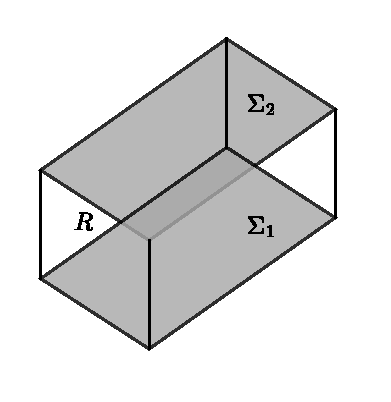
\includegraphics[width=0.72\textwidth]{fig_E.1.pdf}
\caption*{图 E.1\quad 时空中的一个区域 $R$，其空间边界位于无穷远；未来与过去边界包含两个类空超曲面 $\Sigma_1$ 和 $\Sigma_2$。}
\end{figure}

\begin{align*}
0 &= \int_R d(*J) \\
&= \int_{\partial R} *J \\
&= \int_{\Sigma_1} *J - \int_{\Sigma_2} *J \\
&= Q_1 - Q_2.
\tag{E.19}
\end{align*}
第三行中的负号来源于 $\Sigma_2$ 上从 $R$ 继承而来的定向；此时法矢量指向内，与在 $\Sigma_2$ 上积分时惯常的取法恰好相反。我们看到，只要所选的类空超曲面 $\Sigma$ 满足流在无穷远处为零，$Q_\Sigma$ 对任何这样的超曲面都是相同的。这样，Stokes 定理表明了无散（divergenceless）流的存在如何蕴含着一个守恒电荷的存在。

Stokes 定理的另一个用途（对应于三维欧几里得空间中 Gauss 定理的惯常用法）是真正通过在超曲面上积分来算出这个电荷 $Q$。暂时想想真实世界，让我们考虑四维时空中的麦克斯韦方程组。这些方程描述电磁场强张量 $F_{\mu\nu}$ 如何对守恒的电流四矢量作出响应：
\begin{equation*}
\nabla_\mu F^{\nu\mu} = J^\nu.
\tag{E.20}
\end{equation*}
于是我们可以把 $\nabla_\mu F^{\nu\mu}$ 代入式 (E.18) 来计算电荷：
\begin{equation*}
Q = -\int_\Sigma d^3y\,\sqrt{|\gamma|}\,n_\mu\nabla_\nu F^{\mu\nu}.
\tag{E.21}
\end{equation*}
每当遇到一个反对称张量场 $F^{\mu\nu} = -F^{\nu\mu}$ 的散度在超曲面 $\Sigma$ 上的积分时，我们都可以仿照导出式 (E.14) 的步骤，把散度与 $F^{\mu\nu}$ 在边界上的取值联系起来，不过这次是在空间无穷远处（前提是该超曲面是类时的）：
\begin{equation*}
\boxed{\int_\Sigma d^{n-1}y\,\sqrt{|\gamma|}\,n_\mu\nabla_\nu F^{\mu\nu} = \int_{\partial\Sigma} d^{n-2}z\,\sqrt{|\gamma^{(\partial\Sigma)}|}\,n_\mu\sigma_\nu F^{\mu\nu},}
\tag{E.22}
\end{equation*}
其中诸 $z^a$ 是 $\partial\Sigma$ 上的坐标，$\gamma^{(\partial\Sigma)}_{ab}$ 是 $\partial\Sigma$ 上的诱导度规，而 $\sigma^\mu$ 是 $\partial\Sigma$ 的单位法矢量。你可能会担心对 $\partial\Sigma$ 的积分，因为%
% ---- 书页 457 / p472 ----
边界的边界为零；但 $\Sigma$ 并不是任何区域的完整边界，而只是其中一块，所以它当然可以有自己的边界。

为了确认我们清楚自己正在做什么，让我们验证一下确实能在 Minkowski 空间中恢复出一个点粒子的电荷。把度规写成极坐标形式：
\begin{equation*}
ds^2 = -dt^2 + dr^2 + r^2d\theta^2 + r^2\sin^2\theta\,d\phi^2.
\tag{E.23}
\end{equation*}
在我们的单位制下（Lorentz–Heaviside 约定，麦克斯韦方程组中不出现 $4\pi$），电荷 $q$ 的电场为
\begin{equation*}
E^r = \frac{q}{4\pi r^2},
\tag{E.24}
\end{equation*}
其余分量为零；它与场强张量的关系是
\begin{equation*}
F^{tr} = -F^{rt} = E^r.
\tag{E.25}
\end{equation*}
单位法矢量为
\begin{equation*}
n^\mu = (1,\,0,\,0,\,0),\qquad \sigma^\mu = (0,\,1,\,0,\,0),
\tag{E.26}
\end{equation*}
于是
\begin{equation*}
n_\mu\sigma_\nu F^{\mu\nu} = -E^r = -\frac{q}{4\pi r^2}.
\tag{E.27}
\end{equation*}
空间无穷远处二维球面上的度规为
\begin{equation*}
\gamma^{(S^2)}_{ab}\,dz^a dz^b = r^2d\theta^2 + r^2\sin^2\theta\,d\phi^2,
\tag{E.28}
\end{equation*}
所以体积元为
\begin{equation*}
d^2z\sqrt{\gamma^{(S^2)}} = r^2\sin\theta\,d\theta\,d\phi.
\tag{E.29}
\end{equation*}
把式 (E.27)、式 (E.29) 和式 (E.21) 代入式 (E.22)，给出
\begin{align*}
Q &= -\lim_{r\to\infty}\int_{S^2} d\theta\,d\phi\,r^2\sin\theta\left(-\frac{q}{4\pi r^2}\right) \\
&= q,
\tag{E.30}
\end{align*}
这正是我们要找的答案。

% ---- 书页 458 / p473 ----
% （本页为空白页）

% 附录F Geodesic Congruences
\chapter{测地线汇}

% ---- 书页 459 / p474 ----
在 3.10 节中我们导出了测地偏离方程，它支配着连接一个单参数邻近测地线族的分离矢量（separation vector）的演化。要更全面地了解邻近测地线的行为，就不能只考虑单参数族，而要考虑一整个测地线汇（congruence）。线汇是时空开区域中的一组曲线，使得区域中的每一点恰好落在其中一条曲线上。我们可以把测地线汇想象成描画一组互不相互作用的粒子在时空中沿互不相交的路径运动的轨迹。如果测地线相交，线汇就必然在该点终止。显然，在一个多维线汇中有很多信息需要追踪；我们感兴趣的将是单条测地线邻域内的局域行为，对此问题会变得相当容易处理。

令 $U^\mu = dx^\mu/d\tau$ 为一个四维类时测地线汇的切矢量场；等价地说，它是某种无压流体（pressureless fluid）的四速度场。（倘若流体不是无压的，$U^\mu$ 的积分曲线一般就不会描述测地线。）类光测地线会带来一些特殊问题，我们稍后再回来讨论；现在只考虑类时的情形。作为参考，我们回忆一下，这个切矢量场是归一化的，并且满足测地线方程：
\begin{equation*}
U_\mu U^\mu = -1,\qquad U^\lambda\nabla_\lambda U^\mu = 0.
\tag{F.1}
\end{equation*}
在 3.10 节讨论测地偏离方程时，我们考虑了从一个测地线指向邻近测地线的分离矢量 $V^\mu$，并发现它满足
\begin{equation*}
\frac{DV^\mu}{d\tau} \equiv U^\nu\nabla_\nu V^\mu = B^\mu{}_\nu V^\nu,
\tag{F.2}
\end{equation*}
其中
\begin{equation*}
B^\mu{}_\nu = \nabla_\nu U^\mu.
\tag{F.3}
\end{equation*}
（在第 3 章中我们用 $T$ 代替 $U$，用 $S$ 代替 $V$。）因此，张量 $B_{\mu\nu}$ 可以看成是在量度 $V^\mu$ 沿线汇不被平行移动的程度；换言之，它描述的是邻近测地线偏离完全平行的程度。

为了处理一整个线汇而不只是单参数曲线族，我们可以想象架设一组与我们的%
% ---- 书页 460 / p475 ----
类时测地线正交的法矢量，并追踪它们的演化。这一组矢量不被平行移动这一事实，将告诉我们线汇中邻近的测地线如何演化。等价地，我们可以想象在某个点处放置一小球检验粒子，并想要定量描述这些粒子相对于其中心测地线的演化。幸运的是，所有我们需要追踪的只是 $B_{\mu\nu}$ 的行为。

给定矢量场 $U^\mu$，在每一点 $p$ 我们考虑 $T_pM$ 中与 $U^\mu$ 垂直的矢量所对应的子空间。$T_pM$ 中的任何矢量都可以借助投影张量（projection tensor）投影到这个子空间中：
\begin{equation*}
P^\mu{}_\nu = \delta^\mu_\nu + U^\mu U_\nu,
\tag{F.4}
\end{equation*}
这在我们讨论附录 D 的子流形时已经见过。这里我们不是投影到一个子流形上，而只是投影到切空间的一个矢量子空间上，但想法是一样的。我们注意到，$B_{\mu\nu}$ 已经处于法向子空间之中，因为
\begin{align*}
U^\mu B_{\mu\nu} &= U^\mu\nabla_\nu U_\mu = 0 \\
U^\nu B_{\mu\nu} &= U^\nu\nabla_\nu U_\mu = 0.
\tag{F.5}
\end{align*}
其中第一式来自 $\nabla_\nu(U^\mu U_\mu) = \nabla_\nu(-1) = 0$，第二式则来自测地线方程。我们不应把 $B_{\mu\nu}$ 与式 (D.53) 中的外曲率 $K_{\mu\nu}$ 混淆起来；区别在于，我们的切矢量场 $U^\mu$ 一般不会与任何超曲面正交。

作为一个 (0, 2) 型张量，$B_{\mu\nu}$ 可以分解为对称部分与反对称部分，而对称部分还可以进一步分解为迹与无迹（trace-free）部分。由于 $B_{\mu\nu}$ 处于法向子空间中，我们可以用 $P_{\mu\nu}$ 来取这个分解中的迹。结果可以写成
\begin{equation*}
B_{\mu\nu} = \frac{1}{3}\theta P_{\mu\nu} + \sigma_{\mu\nu} + \omega_{\mu\nu}.
\tag{F.6}
\end{equation*}
这里我们引入了三个描述这一分解的量，首先是线汇的\textbf{膨胀}（expansion）$\theta$，
\begin{equation*}
\theta = P^{\mu\nu}B_{\mu\nu} = \nabla_\mu U^\mu,
\tag{F.7}
\end{equation*}
它就是 $B_{\mu\nu}$ 的迹。膨胀描述的是以我们的测地线为中心的检验粒子球的体积变化。它显然是一个标量，这也讲得通，因为体积的整体膨胀/收缩正是由一个单一的数来描述的。\textbf{切变}（shear）$\sigma_{\mu\nu}$ 由下式给出：
\begin{equation*}
\sigma_{\mu\nu} = B_{(\mu\nu)} - \frac{1}{3}\theta P_{\mu\nu}.
\tag{F.8}
\end{equation*}
它是对称且无迹的。切变表示的是检验粒子集合形状上的畸变，即从初始的球变成椭球；其对称性代表了这样一个事实：沿（比方说）$x$ 方向的拉长%
% ---- 书页 461 / p476 ----
与沿 $-x$ 方向的拉长是同一回事。最后是\textbf{转动}（rotation）$\omega_{\mu\nu}$，由下式给出：
\begin{equation*}
\omega_{\mu\nu} = B_{[\mu\nu]}.
\tag{F.9}
\end{equation*}
它是一个反对称张量，这也合乎情理；比如 $xy$ 分量描述的是绕 $z$ 轴的转动，而 $yx$ 分量描述的是绕同一轴反方向的转动。

线汇的演化由这些量沿路径的协变导数 $D/d\tau = U^\sigma\nabla_\sigma$ 来描述。我们可以对整个张量 $B_{\mu\nu}$ 直接进行计算，然后再取相应的分解。我们得到
\begin{align*}
\frac{DB_{\mu\nu}}{d\tau} &\equiv U^\sigma\nabla_\sigma B_{\mu\nu} = U^\sigma\nabla_\sigma\nabla_\nu U_\mu \\
&= U^\sigma\nabla_\nu\nabla_\sigma U_\mu + U^\sigma R^\lambda{}_{\mu\nu\sigma}U_\lambda \\
&= \nabla_\nu(U^\sigma\nabla_\sigma U_\mu) - (\nabla_\nu U^\sigma)(\nabla_\sigma U_\mu) - R_{\lambda\mu\nu\sigma}U^\sigma U^\lambda \\
&= -B^\sigma{}_\nu B_{\mu\sigma} - R_{\lambda\mu\nu\sigma}U^\sigma U^\lambda.
\tag{F.10}
\end{align*}
对这个方程取迹，就得到膨胀的一个演化方程，
\begin{equation*}
\boxed{\frac{d\theta}{d\tau} = -\frac{1}{3}\theta^2 - \sigma_{\mu\nu}\sigma^{\mu\nu} + \omega_{\mu\nu}\omega^{\mu\nu} - R_{\mu\nu}U^\mu U^\nu.}
\tag{F.11}
\end{equation*}
这就是 Raychaudhuri 方程，它在奇点定理的证明中起着关键作用。【有时也放弃线汇必须服从测地线方程的要求；这不过是在右边额外添加一项 $\nabla_\mu(U^\nu\nabla_\nu U^\mu)$ 而已。】类似地，式 (F.10) 的对称无迹部分为
\begin{align*}
\frac{D\sigma_{\mu\nu}}{d\tau} &= -\frac{2}{3}\theta\sigma_{\mu\nu} - \sigma_{\mu\alpha}\sigma^\alpha{}_\nu - \omega_{\mu\rho}\omega^\rho{}_\nu + \frac{1}{3}P_{\mu\nu}\left(\sigma_{\alpha\beta}\sigma^{\alpha\beta} - \omega_{\alpha\beta}\omega^{\alpha\beta}\right) \\
&\quad + C_{\alpha\nu\mu\beta}U^\alpha U^\beta + \frac{1}{2}\bar{R}_{\mu\nu},
\tag{F.12}
\end{align*}
其中 $\bar{R}_{\mu\nu}$ 是 $R_{\mu\nu}$ 经空间投影后的无迹部分，
\begin{equation*}
\bar{R}_{\mu\nu} = P^\alpha{}_\mu P^\beta{}_\nu R_{\alpha\beta} - \frac{1}{3}P_{\mu\nu}P^{\alpha\beta}R_{\alpha\beta},
\tag{F.13}
\end{equation*}
而式 (F.10) 的反对称部分为
\begin{equation*}
\frac{D\omega_{\mu\nu}}{d\tau} = -\frac{2}{3}\theta\omega_{\mu\nu} + \sigma_\mu{}^\alpha\omega_{\nu\alpha} - \sigma_\nu{}^\alpha\omega_{\mu\alpha}.
\tag{F.14}
\end{equation*}
这些方程用得不像 Raychaudhuri 方程那样频繁，但有它们在手总是好事。

% ---- 书页 462 / p477 ----
让我们简要举一个 Raychaudhuri 方程用法的例子。首先注意到，由于切变和转动都是“空间的”张量，我们有
\begin{equation*}
\sigma_{\mu\nu}\sigma^{\mu\nu} \geq 0,\qquad \omega_{\mu\nu}\omega^{\mu\nu} \geq 0.
\tag{F.15}
\end{equation*}
其次注意到，式 (F.11) 中的最后一项，恰恰就是把 Einstein 方程与强能量条件（Strong Energy Condition, SEC）结合起来时所出现的那一项；由 Einstein 方程我们知道
\begin{equation*}
R_{\mu\nu}U^\mu U^\nu = 8\pi G\left(T_{\mu\nu} - \frac{1}{2}Tg_{\mu\nu}\right)U^\mu U^\nu,
\tag{F.16}
\end{equation*}
而强能量条件要求这个表达式的右边对任何类时 $U^\mu$ 都非负。于是我们有
\begin{equation*}
R_{\mu\nu}U^\mu U^\nu \geq 0
\tag{F.17}
\end{equation*}
倘若强能量条件成立。最后注意到，$\omega_{\mu\nu} = 0$ 当且仅当矢量场 $U^\mu$ 与一族超曲面正交。这可以直接从如下事实得到：转动是一个空间张量（$U^\mu\omega_{\mu\nu} = 0$），而由 Frobenius 定理，矢量场 $U^\mu$ 超曲面正交（hypersurface-orthogonal）的充要条件是 $U_{[\mu}\nabla_\nu U_{\rho]}$；细节留给大家自行核验。因此，如果我们有一个切矢量场超曲面正交的线汇，而时空又服从 Einstein 方程和强能量条件，则 Raychaudhuri 方程蕴含
\begin{equation*}
\frac{d\theta}{d\tau} \leq -\frac{1}{3}\theta^2.
\tag{F.18}
\end{equation*}
这个方程容易积分，得到
\begin{equation*}
\theta^{-1}(\tau) \geq \theta_0^{-1} + \frac{1}{3}\tau.
\tag{F.19}
\end{equation*}
考虑一个超曲面正交的线汇，它初始时是会聚的（$\theta_0 < 0$）而不是膨胀的。那么式 (F.19) 告诉我们，会聚将持续下去，并且我们必然在有限固有时 $\tau \leq -3\theta_0^{-1}$ 内碰到一个焦散（caustic，即测地线相交之处）。换言之，服从强能量条件的物质永远不可能开始把测地线推开，它只会增大测地线会聚的速率。当然，这个结果只适用于某个任意选定的线汇，而且焦散的出现肯定不代表时空中存在任何奇点（测地线时时刻刻都在相交，即便在平直时空中也是如此）。但奇点定理的许多证明正是利用 Raychaudhuri 方程的这一性质，来证明时空必定在某种意义上测地不完备。

接下来我们转向类光测地线汇的行为。这要更棘手一些，根本原因在于我们的出发点（研究切矢量场法向的三维子空间中矢量的演化）不再那么有意义，因为类光曲线的切矢量与它自身正交。相反，在类光情形下我们关心的是这样的二维子空间中矢量的演化：它由与类光切矢量场 $k^\mu = dx^\mu/d\lambda$ 正交的“空间”矢量组成。

% ---- 书页 463 / p478 ----
遗憾的是，定义这个子空间并没有唯一的方法，因为处于不同洛伦兹系中的观者对什么算作空间矢量有不同的看法。面对这一困境，我们有两种说得过去的做法。一种巧妙的做法，是从与 $k^\mu$ 正交的三维矢量空间出发，取等价类——两个矢量若相差 $k^\mu$ 的倍数就算等价——由此定义一个抽象的二维矢量空间。另一种比较笨拙的做法（我们将采用的就是这一种），则是干脆再选一个“辅助”（auxiliary）类光矢量 $l^\mu$，它（在某个参考系中）指向与 $k^\mu$ 相反的空间方向，并归一化为
\begin{equation*}
l^\mu l_\mu = 0,\qquad l^\mu k_\mu = -1.
\tag{F.20}
\end{equation*}
我们进一步要求这个辅助矢量是被平行移动的：
\begin{equation*}
k^\mu\nabla_\mu l^\nu = 0,
\tag{F.21}
\end{equation*}
这与式 (F.20) 相容，因为平行移动保持内积。辅助类光矢量 $l^\mu$ 绝不是唯一的，因为我们刚刚指出，“指向相反的空间方向”这一概念依赖于参考系。尽管如此，我们可以作出一个选择，并希望重要的量不依赖于这个任意的选取。这样做了之后，我们感兴趣的二维法向矢量空间记作 $T_\perp$，它恰好由与 $k^\mu$ 和 $l^\mu$ 都正交的那些矢量 $V^\mu$ 组成：
\begin{equation*}
T_\perp = \{V^\mu \mid V^\mu k_\mu = 0,\, V^\mu l_\mu = 0\}.
\tag{F.22}
\end{equation*}
我们现在的任务，就是追踪生活在这个子空间中的偏离矢量（它们代表一族邻近的类光测地线）的演化。

投影到法向子空间 $T_\perp$ 需要对投影张量的定义稍作修改；结果发现
\begin{equation*}
Q_{\mu\nu} = g_{\mu\nu} + k_\mu l_\nu + k_\nu l_\mu
\tag{F.23}
\end{equation*}
就能奏效。也就是说，作用在 $T_\perp$ 中的矢量 $V^\mu$、$W^\mu$ 上时，$Q_{\mu\nu}$ 的表现如同度规，而作用在任何与 $k^\mu$ 或 $l^\mu$ 成比例的东西上都给出零。这个投影张量的一些有用性质包括
\begin{gather*}
Q_{\mu\nu}V^\mu W^\nu = g_{\mu\nu}V^\mu W^\nu \\
Q^\mu{}_\nu V^\nu = V^\mu \\
Q^\mu{}_\nu k^\nu = 0 \\
Q^\mu{}_\nu l^\nu = 0 \\
Q^\mu{}_\nu Q^\nu{}_\sigma = Q^\mu{}_\sigma \\
k^\sigma\nabla_\sigma Q^\mu{}_\nu = 0.
\tag{F.24}
\end{gather*}
（译注：原书第一行左端印作 $Q_{\mu\nu}V^\nu W^\nu$，指标显然误排，现按右端之意改为 $V^\mu W^\nu$。）

% ---- 书页 464 / p479 ----
正如类时测地线的情形，法向偏离矢量 $V^\mu$ 不被平行传播，由张量 $B^\mu{}_\nu = \nabla_\nu k^\mu$ 支配，具体说来就是
\begin{equation*}
\frac{DV^\mu}{d\lambda} \equiv k^\nu\nabla_\nu V^\mu = B^\mu{}_\nu V^\nu.
\tag{F.25}
\end{equation*}
然而，在类光情形下，张量 $B_{\mu\nu}$ 实际上超出了我们的需要；相关信息完全包含在投影之后的版本中，
\begin{equation*}
\widehat{B}^\mu{}_\nu = Q^\mu{}_\alpha Q^\beta{}_\nu B^\alpha{}_\beta.
\tag{F.26}
\end{equation*}
要看清这一点，我们只需摆弄一下式 (F.25)，并用上式 (F.24) 中的各条性质：
\begin{align*}
\frac{DV^\mu}{d\lambda} &= k^\nu\nabla_\nu V^\mu \\
&= k^\nu\nabla_\nu(Q^\mu{}_\rho V^\rho) \\
&= Q^\mu{}_\rho k^\nu\nabla_\nu V^\rho \\
&= Q^\mu{}_\rho B^\rho{}_\nu V^\nu \\
&= Q^\mu{}_\rho B^\rho{}_\nu Q^\nu{}_\sigma V^\sigma \\
&= \widehat{B}^\mu{}_\sigma V^\sigma.
\tag{F.27}
\end{align*}
所以我们只需追踪这个投影后张量的演化，而不必理会完整的 $B_{\mu\nu}$。

为了理解这一演化，我们再次把它分解成膨胀、切变和转动：
\begin{equation*}
\widehat{B}_{\mu\nu} = \frac{1}{2}\theta Q_{\mu\nu} + \widehat{\sigma}_{\mu\nu} + \widehat{\omega}_{\mu\nu},
\tag{F.28}
\end{equation*}
其中
\begin{gather*}
\theta = Q^{\mu\nu}\widehat{B}_{\mu\nu} = \widehat{B}^\mu{}_\mu \\
\widehat{\sigma}_{\mu\nu} = \widehat{B}_{(\mu\nu)} - \frac{1}{2}\theta Q_{\mu\nu} \\
\widehat{\omega}_{\mu\nu} = \widehat{B}_{[\mu\nu]}.
\tag{F.29}
\end{gather*}
我们这里出现的是因子 $1/2$ 而不是 $1/3$，因为我们的法向空间 $T_\perp$ 是二维的，这也体现在 $Q^{\mu\nu}Q_{\mu\nu} = 2$ 这一事实之中。与类时情形一样，$\widehat{\omega}_{\mu\nu} = 0$ 是线汇超曲面正交的充要条件。$\widehat{B}_{\mu\nu}$ 沿路径的演化由下式给出：
\begin{align*}
\frac{D\widehat{B}_{\mu\nu}}{d\lambda} &\equiv k^\sigma\nabla_\sigma\widehat{B}_{\mu\nu} = k^\sigma\nabla_\sigma(Q^\alpha{}_\mu Q^\beta{}_\nu\nabla_\alpha k_\beta) \\
&= Q^\alpha{}_\mu Q^\beta{}_\nu k^\sigma\nabla_\sigma\nabla_\alpha k_\beta \\
% ---- 书页 465 / p480 ----
&= -Q^\alpha{}_\mu Q^\beta{}_\nu\left(B_\alpha{}^\sigma B_{\beta\sigma} + R_{\alpha\lambda\beta\sigma}k^\lambda k^\sigma\right) \\
&= -\widehat{B}_\mu{}^\sigma\widehat{B}_{\nu\sigma} - Q^\alpha{}_\mu Q^\beta{}_\nu R_{\alpha\lambda\beta\sigma}k^\lambda k^\sigma.
\tag{F.30}
\end{align*}
（译注：原书 (F.30) 末行曲率项印作 $R_{\mu\lambda\nu\sigma}$，但这样与其前面的 $Q^\alpha{}_\mu Q^\beta{}_\nu$ 相配则指标失衡；按上行的 $R_{\alpha\lambda\beta\sigma}$ 改正。）

继续沿着我们以前的逻辑，对这个方程取迹，就可以得到类光测地线膨胀的演化方程，
\begin{equation*}
\frac{d\theta}{d\lambda} = -\frac{1}{2}\theta^2 - \widehat{\sigma}_{\mu\nu}\widehat{\sigma}^{\mu\nu} + \widehat{\omega}_{\mu\nu}\widehat{\omega}^{\mu\nu} - R_{\mu\nu}k^\mu k^\nu.
\tag{F.31}
\end{equation*}
令人欣喜的是，这个方程最终与我们任意选定的辅助矢量 $l^\mu$ 完全无关。首先，膨胀本身就与 $l^\mu$ 无关，这很容易验证：
\begin{align*}
\theta &= Q^{\mu\nu}\widehat{B}_{\mu\nu} \\
&= Q^{\mu\nu}B_{\mu\nu} \\
&= g^{\mu\nu}B_{\mu\nu},
\tag{F.32}
\end{align*}
其中第二步用了 $Q^{\mu\nu}Q^\alpha{}_\nu = Q^{\mu\alpha}$，第三步用了 $k^\mu B_{\mu\nu} = k^\nu B_{\mu\nu} = 0$。（这就是为什么我们从头到尾都不必给 $\theta$ 戴帽子。）其次，$\widehat{\sigma}_{\mu\nu}\widehat{\sigma}^{\mu\nu}$ 与 $\widehat{\omega}_{\mu\nu}\widehat{\omega}^{\mu\nu}$ 同样与 $l^\mu$ 无关（欢迎大家自行验证），尽管 $\widehat{\sigma}_{\mu\nu}$ 和 $\widehat{\omega}_{\mu\nu}$ 本身并非如此。最后，在取迹时，投影张量从曲率张量那一项中消失了。因此，我们得到了关于膨胀演化的一个良定义的概念，它与我们作出的任何任意选择无关。注意到，由于 $k^\mu$ 是类光的，Einstein 方程蕴含
\begin{align*}
R_{\mu\nu}k^\mu k^\nu &= 8\pi G\left(T_{\mu\nu} - \frac{1}{2}Tg_{\mu\nu}\right)k^\mu k^\nu \\
&= 8\pi G T_{\mu\nu}k^\mu k^\nu.
\tag{F.33}
\end{align*}
要使它非负，我们只需援引类光能量条件（Null Energy Condition）——在第 3 章讨论过的所有能量条件中，这是限制最弱的一个。于是，与类时测地线相比，类光测地线在更一般的条件下就会会聚成焦散。

我们还可以继续下去，得到切变的演化方程，
\begin{equation*}
\frac{D\widehat{\sigma}_{\mu\nu}}{d\lambda} = -\theta\widehat{\sigma}_{\mu\nu} - Q^\alpha{}_\mu Q^\beta{}_\nu C_{\alpha\lambda\beta\sigma}k^\lambda k^\sigma,
\tag{F.34}
\end{equation*}
（译注：原书此式曲率项印作 $C_{\mu\lambda\nu\sigma}$，与 $Q^\alpha{}_\mu Q^\beta{}_\nu$ 相配则指标失衡，现按 (F.30) 同样的思路改为 $C_{\alpha\lambda\beta\sigma}$。）
以及转动的演化方程，
\begin{equation*}
\frac{D\widehat{\omega}_{\mu\nu}}{d\lambda} = -\theta\widehat{\omega}_{\mu\nu}.
\tag{F.35}
\end{equation*}
这些方程不如膨胀的那个方程来得自然，因为切变和转动确实依赖于我们对 $l^\mu$ 的选取；尽管如此，在具体情形中它们仍然可能有用。

% ---- 书页 466 / p481 ----
% （本页为空白页）

% 附录G Conformal Transformations

\chapter{共形变换}

% ---- 书页 467 / p482 ----
\textbf{共形变换}（conformal transformation）本质上是一种局部的标度改变。由于距离是靠度规来量度的，这类变换是通过用一个依赖于时空位置的（非零）函数去乘度规来实现的：
\begin{equation*}
\tilde{g}_{\mu\nu} = \omega^{2}(x) g_{\mu\nu},
\tag{G.1}
\end{equation*}
或等价地
\begin{equation*}
\widetilde{ds}^{2} = \omega^{2}(x) ds^{2},
\tag{G.2}
\end{equation*}
其中 $\omega(x)$ 是某个非零函数。（这里用 $x$ 表示时空坐标 $x^{\mu}$ 的全体。）注意，逆共形变换是平凡的：$g_{\mu\nu} = \omega^{-2}\tilde{g}_{\mu\nu}$。这类变换在广义相对论中有许多用途；我们最钟爱的两个用途是：在标量-张量理论中更换动力学变量（如 4.8 节所述），以及把时空重新映射成便于使用的共形图（见下一个附录）。

我们首先指出一个关键事实：\emph{类光曲线在共形变换下保持不变}。这句话的意思很简单：如果 $x^{\mu}(\lambda)$ 是一条关于 $g_{\mu\nu}$ 为类光的曲线，那么它关于 $\tilde{g}_{\mu\nu}$ 也是类光的。只要我们明白“曲线 $x^{\mu}(\lambda)$ 为类光，当且仅当它的切矢量 $\mathrm{d}x^{\mu}/\mathrm{d}\lambda$ 为类光”，这一点便立即得证：
\begin{equation*}
g_{\mu\nu}\frac{dx^{\mu}}{d\lambda}\frac{dx^{\nu}}{d\lambda} = 0.
\tag{G.3}
\end{equation*}
于是，在与它共形相关的度规中，我们有
\begin{equation*}
\tilde{g}_{\mu\nu}\frac{dx^{\mu}}{d\lambda}\frac{dx^{\nu}}{d\lambda}
= \omega^{2}(x) g_{\mu\nu}\frac{dx^{\mu}}{d\lambda}\frac{dx^{\nu}}{d\lambda} = 0.
\tag{G.4}
\end{equation*}
这样，按一个度规定义为类光的曲线，按任何与它共形相关的度规定义也是类光的。我们可以说，“共形变换保持光锥不变。”（事实上，你可以验证它们也保持任意两个四维矢量之间的夹角不变；我们的共形变换与复分析中人们熟悉的共形变换正共享这一特点。）

接下来让我们考虑几何量在共形变换下如何改变。共形变换不是坐标变换，而是几何本身的实际改变——例如，$\tilde{g}_{\mu\nu}$ 的类时测地线一般会不同于 $g_{\mu\nu}$ 的类时测地线。不过，我们可以利用共形变换来更换动力学变量：任何作为 $g_{\mu\nu}$ 的函数的量，都同样可以看作 $\tilde{g}_{\mu\nu}$ 与 $\omega(x)$ 的函数。这时我们说这些量被表达在\textbf{共形框架}（conformal frame）之中。在本附录里，我们汇集一些表达式，说明原度规 $g_{\mu\nu}$ 中的各量如何与共形度规 $\tilde{g}_{\mu\nu}$ 中的各量相联系。

% ---- 书页 468 / p483 ----
我们先从 Christoffel 符号开始考察。由于联络系数对度规的导数是线性的，对逆度规也是线性的，经共形变换后的联络具有如下形式：
\begin{equation*}
\widetilde{\Gamma}^{\rho}{}_{\mu\nu} = \Gamma^{\rho}{}_{\mu\nu} + C^{\rho}{}_{\mu\nu}.
\tag{G.5}
\end{equation*}
$C^{\rho}{}_{\mu\nu}$ 显然是一个张量，因为它是两个联络之差。显式计算表明它由下式给出：
\begin{equation*}
C^{\rho}{}_{\mu\nu} = \omega^{-1}\left(\delta^{\rho}_{\mu}\nabla_{\nu}\omega + \delta^{\rho}_{\nu}\nabla_{\mu}\omega - g_{\mu\nu}g^{\rho\lambda}\nabla_{\lambda}\omega\right).
\tag{G.6}
\end{equation*}
当我们考虑 Riemann 张量在共形变换下的行为时，这个公式立刻就派上了用场。事实上，对任何形如式 (G.5) 的联络改变，我们都有
\begin{equation*}
\widetilde{R}^{\rho}{}_{\sigma\mu\nu} = R^{\rho}{}_{\sigma\mu\nu} + \nabla_{\mu}C^{\rho}{}_{\nu\sigma} - \nabla_{\nu}C^{\rho}{}_{\mu\sigma} + C^{\rho}{}_{\mu\lambda}C^{\lambda}{}_{\nu\sigma} - C^{\rho}{}_{\nu\lambda}C^{\lambda}{}_{\mu\sigma}.
\tag{G.7}
\end{equation*}
于是，只需代入并埋头演算，就得到
\begin{align*}
\widetilde{R}^{\rho}{}_{\sigma\mu\nu} = R^{\rho}{}_{\sigma\mu\nu} &- 2\left(\delta^{\rho}_{[\mu}\delta^{\alpha}_{\nu]}\delta^{\beta}_{\sigma} - g_{\sigma[\mu}\delta^{\alpha}_{\nu]}g^{\rho\beta}\right)\omega^{-1}(\nabla_{\alpha}\nabla_{\beta}\omega) \\
&+ 2\left(2\delta^{\rho}_{[\mu}\delta^{\alpha}_{\nu]}\delta^{\beta}_{\sigma} - 2g_{\sigma[\mu}\delta^{\alpha}_{\nu]}g^{\rho\beta} + g_{\sigma[\mu}\delta^{\rho}_{\nu]}g^{\alpha\beta}\right)\omega^{-2}(\nabla_{\alpha}\omega)(\nabla_{\beta}\omega).
\tag{G.8}
\end{align*}
把第一个和第三个指标缩并，就得到 Ricci 张量，
\begin{align*}
\widetilde{R}_{\sigma\nu} = R_{\sigma\nu} &- \left[(n-2)\delta^{\alpha}_{\sigma}\delta^{\beta}_{\nu} + g_{\sigma\nu}g^{\alpha\beta}\right]\omega^{-1}(\nabla_{\alpha}\nabla_{\beta}\omega) \\
&+ \left[2(n-2)\delta^{\alpha}_{\sigma}\delta^{\beta}_{\nu} - (n-3)g_{\sigma\nu}g^{\alpha\beta}\right]\omega^{-2}(\nabla_{\alpha}\omega)(\nabla_{\beta}\omega),
\tag{G.9}
\end{align*}
其中 $n$ 是维数。提升一个指标（利用 $\tilde{g}^{\mu\nu} = \omega^{-2}g^{\mu\nu}$）并再作一次缩并，就得到标量曲率，
\begin{equation*}
\widetilde{R} = \omega^{-2}R - 2(n-1)g^{\alpha\beta}\omega^{-3}(\nabla_{\alpha}\nabla_{\beta}\omega) - (n-1)(n-4)g^{\alpha\beta}\omega^{-4}(\nabla_{\alpha}\omega)(\nabla_{\beta}\omega).
\tag{G.10}
\end{equation*}
另一个有用的量是标量场 $\phi$ 的协变导数。一阶协变导数在原框架与共形框架中是相等的，因为二者都等于偏导数：
\begin{equation*}
\widetilde{\nabla}_{\mu}\phi = \nabla_{\mu}\phi = \partial_{\mu}\phi.
\tag{G.11}
\end{equation*}

% ---- 书页 469 / p484 ----
不过，二阶导数涉及 Christoffel 符号，因此具有非平凡的变换律：
\begin{equation*}
\widetilde{\nabla}_{\mu}\widetilde{\nabla}_{\nu}\phi = \nabla_{\mu}\nabla_{\nu}\phi - \left(\delta^{\alpha}_{\mu}\delta^{\beta}_{\nu} + \delta^{\beta}_{\mu}\delta^{\alpha}_{\nu} - g_{\mu\nu}g^{\alpha\beta}\right)\omega^{-1}(\nabla_{\alpha}\omega)(\nabla_{\beta}\phi).
\tag{G.12}
\end{equation*}
我们可以用 $\tilde{g}^{\mu\nu}$ 对它缩并，得到 d'Alembert 算符，
\begin{equation*}
\widetilde{\Box}\phi = \omega^{-2}\Box\phi + (n-2)g^{\alpha\beta}\omega^{-3}(\nabla_{\alpha}\omega)(\nabla_{\beta}\phi).
\tag{G.13}
\end{equation*}
最后，我们也许想反其道而行，用共形度规来表达原度规中的各个量。这不过是件繁琐的计算活儿；为方便起见，这里把答案抄录如下。曲率张量及其缩并为
\begin{align*}
R^{\rho}{}_{\sigma\mu\nu} = \widetilde{R}^{\rho}{}_{\sigma\mu\nu} &+ 2\left(\delta^{\rho}_{[\mu}\delta^{\alpha}_{\nu]}\delta^{\beta}_{\sigma} - \tilde{g}_{\sigma[\mu}\delta^{\alpha}_{\nu]}\tilde{g}^{\rho\beta}\right)\omega^{-1}(\widetilde{\nabla}_{\alpha}\widetilde{\nabla}_{\beta}\omega) \\
&+ 2\tilde{g}_{\sigma[\mu}\delta^{\rho}_{\nu]}\tilde{g}^{\alpha\beta}\,\omega^{-2}(\widetilde{\nabla}_{\alpha}\omega)(\widetilde{\nabla}_{\beta}\omega),
\tag{G.14}
\end{align*}
\begin{align*}
R_{\sigma\nu} = \widetilde{R}_{\sigma\nu} &+ \left[(n-2)\delta^{\alpha}_{\sigma}\delta^{\beta}_{\nu} + \tilde{g}_{\sigma\nu}\tilde{g}^{\alpha\beta}\right]\omega^{-1}(\widetilde{\nabla}_{\alpha}\widetilde{\nabla}_{\beta}\omega) \\
&- (n-1)\tilde{g}_{\sigma\nu}\tilde{g}^{\alpha\beta}\,\omega^{-2}(\widetilde{\nabla}_{\alpha}\omega)(\widetilde{\nabla}_{\beta}\omega),
\tag{G.15}
\end{align*}
以及
\begin{equation*}
R = \omega^{2}\widetilde{R} + 2(n-1)\tilde{g}^{\alpha\beta}\omega(\widetilde{\nabla}_{\alpha}\widetilde{\nabla}_{\beta}\omega) - n(n-1)\tilde{g}^{\alpha\beta}(\widetilde{\nabla}_{\alpha}\omega)(\widetilde{\nabla}_{\beta}\omega),
\tag{G.16}
\end{equation*}
而标量场的协变导数则由下式给出：
\begin{equation*}
\nabla_{\mu}\nabla_{\nu}\phi = \widetilde{\nabla}_{\mu}\widetilde{\nabla}_{\nu}\phi + \left(\delta^{\alpha}_{\mu}\delta^{\beta}_{\nu} + \delta^{\beta}_{\mu}\delta^{\alpha}_{\nu} - \tilde{g}_{\mu\nu}\tilde{g}^{\alpha\beta}\right)\omega^{-1}(\widetilde{\nabla}_{\alpha}\omega)(\widetilde{\nabla}_{\beta}\phi)
\tag{G.17}
\end{equation*}
以及
\begin{equation*}
\Box\phi = \omega^{2}\widetilde{\Box}\phi - (n-2)\tilde{g}^{\alpha\beta}\omega(\widetilde{\nabla}_{\alpha}\omega)(\widetilde{\nabla}_{\beta}\phi).
\tag{G.18}
\end{equation*}

\section{习题}

% 习题编号照原书
\textbf{1.}\quad 证明共形变换保持类光测地线不变，也就是说，$g_{\mu\nu}$ 的类光测地线与 $\omega^{2}g_{\mu\nu}$ 的类光测地线相同。（我们已经知道它们保持类光\emph{曲线}不变；你还需要证明变换后的曲线仍然是测地线。）原度规与共形度规中的仿射参量之间是什么关系？

\textbf{2.}\quad 证明在二维情形下，总能找到一个共形变换（只要算符 $\nabla^{\mu}\nabla_{\mu}$ 可逆），使得变换后的度规的曲率至少在某个坐标卡片中为零。（一般无法在整个流形上同时做到这一点。）这意味着任何二维度规都可以局部地写成一个平直度规乘以一个共形因子。

\textbf{3.}\quad 假设两个度规由如下形式的整体共形变换相联系：
\begin{equation*}
\tilde{g}_{\mu\nu} = e^{\alpha(x)} g_{\mu\nu}.
\tag{G.19}
\end{equation*}

% ---- 书页 470 / p485 ----
\textbf{(a)}\quad 证明：如果 $\xi^{\mu}$ 是度规 $g_{\mu\nu}$ 的一个 Killing 矢量，那么它是度规 $\tilde{g}_{\mu\nu}$ 的一个共形 Killing 矢量。\textbf{共形 Killing 矢量}（conformal Killing vector）满足方程
\begin{equation*}
\nabla_{\mu}\xi_{\nu} + \nabla_{\nu}\xi_{\mu} = (\nabla_{\lambda}\alpha)\xi^{\lambda} g_{\mu\nu}.
\tag{G.20}
\end{equation*}

\textbf{(b)}\quad 证明 $\xi_{\mu}k^{\mu}$ 沿 $\tilde{g}_{\mu\nu}$ 中的光子测地线为常数。这里 $k^{\mu}$ 是光子的四维动量。

\textbf{(c)}\quad 证明共形时间 $\eta = \int dt/R(t)$ 与一个共形 Killing 矢量 $\xi = \partial_{\eta}$ 相联系。

\textbf{(d)}\quad 利用（c）小题重新导出尺度因子与红移之间的关系。

% 附录H Conformal Diagrams
\chapter{共形图}

% ---- 书页 471 / p486 ----
弯曲时空流形原则上可以复杂得超乎想象；幸运的是，我们常常可以用具有高度对称性（尤其是球对称性）的流形来近似物理上现实的情形。然而，即便是对称的时空，如果我们试图想象这类流形的整体结构，它们也会对我们的直观想象能力构成可怕的挑战。因此，能够画出一种标准化的时空图，用来刻画足够对称的时空的整体性质与因果结构，是很有用的。（所谓“因果结构”，指的是由光锥定义的不同事件的过去与未来之间的关系。）\textbf{共形图}（conformal diagrams，亦称 Carter--Penrose 图，或干脆叫彭罗斯图）优雅地实现了这一愿望。

共形图不过是一张普通的时空图，只不过我们对其度规实施了一个特别聪明的坐标变换。由于我们的目标是描绘时空的因果结构，而因果结构由光锥定义，所谓“聪明”，就是指新坐标 $x^{\mu'}$ 具有“类时”坐标与“径向”坐标，且径向光锥在时空图上可以始终如一地画成 $45^{\circ}$。此外，我们追求的是使“无限远”只离有限坐标值之遥的坐标，好让整个时空的结构一目了然。

正如前一个附录中所解释的，共形变换保持光锥不变。既然我们想找到光锥成 $45^{\circ}$ 的坐标，我们只需找到这样一组坐标，使得所关心的度规与另一个我们已知其光锥成 $45^{\circ}$ 的度规共形相关。（当然，光锥画成什么角度取决于我们所用的单位，或者说取决于我们如何画坐标轴；我们真正的意思，是取一组坐标 $T$、$R$，使得径向类光线满足 $dT/dR = \pm 1$。）

让我们从 Minkowski 空间开始，看看这个技巧如何施展。极坐标下的 Minkowski 度规为
\begin{equation*}
ds^{2} = -\mathrm{d}t^{2} + \mathrm{d}r^{2} + r^{2}d\Omega^{2},
\tag{H.1}
\end{equation*}
其中 $d\Omega^{2} = \mathrm{d}\theta^{2} + \sin^{2}\theta\,\mathrm{d}\phi^{2}$ 是单位二维球面上的度规。在这里，我们其实已经可以在每一处都把光锥画成 $45^{\circ}$（轨迹 $t = \pm r$ 是类光的），但我们希望通过换用取值范围有限的坐标，让整个时空的因果结构更加清晰。$\theta$、$\phi$ 坐标不会有什么异样，但我们会想仔细记下另外两个坐标的取值范围。

% ---- 书页 472 / p487 ----
首先当然有
\begin{equation*}
-\infty < t < \infty, \qquad 0 \le r < \infty.
\tag{H.2}
\end{equation*}
严格说来，世界线 $r = 0$ 代表一个坐标奇点，本应由另一张片（patch）来覆盖；但大家都明白这是怎么回事，所以我们就索性装作 $r = 0$ 表现良好。

第一种尝试（结果发现行不通）也许就是简单地重新缩放类时坐标与径向坐标，让它们覆盖一个有限的范围。一个不错的候选是利用反正切函数（如图 H.1 所示），定义 $\bar{t} = \arctan t$、$\bar{r} = \arctan r$。这样度规将取如下形式［利用 $\mathrm{d}\tan x = (1/\cos^{2}x)\mathrm{d}x$］：
\begin{equation*}
ds^{2} = -\frac{1}{\cos^{4}\bar{t}}\,\mathrm{d}\bar{t}^{2} + \frac{1}{\cos^{4}\bar{r}}\,\mathrm{d}\bar{r}^{2} + \tan^{2}\bar{r}\,d\Omega^{2},
\tag{H.3}
\end{equation*}
其取值范围为
\begin{equation*}
\begin{gathered}
-\frac{\pi}{2} < \bar{t} < \frac{\pi}{2} \\
0 \le \bar{r} < \frac{\pi}{2}.
\end{gathered}
\tag{H.4}
\end{equation*}
好消息是新坐标的取值范围有限；坏消息是光锥的斜率（由 $\mathrm{d}\bar{t}/\mathrm{d}\bar{r} = \pm\cos^{2}\bar{t}/\cos^{2}\bar{r}$ 给出）并不像我们希望的那样等于 $\pm 1$。如果我们据此画出相应的时空图（你不妨画着玩玩），类光线走的是哪条路将无从辨认，在时空的边缘处尤其如此。

走出这条死胡同的办法是：不再直来直去地摆弄原坐标 $t$ 和 $r$，而是变得更聪明一点，改用类光坐标：
\begin{equation*}
\begin{aligned}
u &= t - r \\
v &= t + r,
\end{aligned}
\tag{H.5}
\end{equation*}

\begin{figure}[H]
\centering
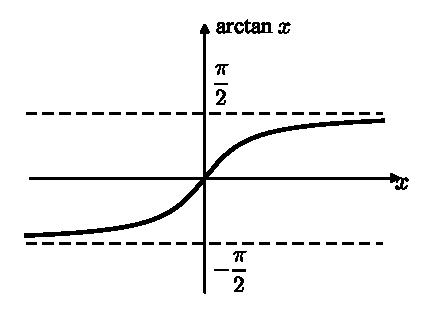
\includegraphics[width=0.72\textwidth]{fig_H.1.pdf}
\caption*{图 H.1\quad 反正切函数把实线映射到一个有限区间。}
\end{figure}

% ---- 书页 473 / p488 ----
\begin{figure}[H]
\centering
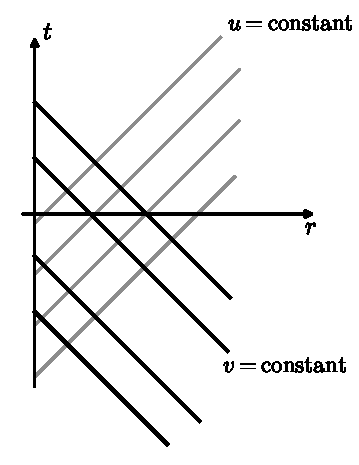
\includegraphics[width=0.72\textwidth]{fig_H.2.pdf}
\caption*{图 H.2\quad Minkowski 空间上的类光径向坐标。}
\end{figure}

其相应的取值范围为
\begin{equation*}
-\infty < u < \infty, \qquad -\infty < v < \infty, \qquad u \le v.
\tag{H.6}
\end{equation*}
这些坐标如图 H.2 所示，图中每个点代表一个半径为 $r = \frac{1}{2}(v-u)$ 的二维球面。类光坐标下的 Minkowski 度规为
\begin{equation*}
ds^{2} = -\frac{1}{2}(\mathrm{d}u\,\mathrm{d}v + \mathrm{d}v\,\mathrm{d}u) + \frac{1}{4}(v-u)^{2}d\Omega^{2}.
\tag{H.7}
\end{equation*}
现在我们利用反正切把无限远拉到有限的坐标值处，令
\begin{equation*}
\begin{aligned}
U &= \arctan u \\
V &= \arctan v,
\end{aligned}
\tag{H.8}
\end{equation*}
其取值范围为
\begin{equation*}
-\pi/2 < U < \pi/2, \qquad -\pi/2 < V < \pi/2, \qquad U \le V.
\tag{H.9}
\end{equation*}
于是我们有
\begin{equation*}
\mathrm{d}u\,\mathrm{d}v + \mathrm{d}v\,\mathrm{d}u = \frac{1}{\cos^{2}U\cos^{2}V}(\mathrm{d}U\,\mathrm{d}V + \mathrm{d}V\,\mathrm{d}U),
\tag{H.10}
\end{equation*}
以及
\begin{align*}
(v-u)^{2} &= (\tan V - \tan U)^{2} = \frac{1}{\cos^{2}U\cos^{2}V}\left(\sin V\cos U - \cos V\sin U\right)^{2} \\
&= \frac{1}{\cos^{2}U\cos^{2}V}\sin^{2}(V-U),
\tag{H.11}
\end{align*}

% ---- 书页 474 / p489 ----
于是度规式 (H.7) 在这些坐标下成为
\begin{equation*}
ds^{2} = \frac{1}{4\cos^{2}U\cos^{2}V}\left[-2(\mathrm{d}U\,\mathrm{d}V + \mathrm{d}V\,\mathrm{d}U) + \sin^{2}(V-U)\,d\Omega^{2}\right].
\tag{H.12}
\end{equation*}
这种形式有一定的魅力，因为度规看起来就像一个相当简单的表达式乘以一个整体因子。我们还可以更进一步，通过如下变换回到一个类时坐标 $T$ 与一个径向坐标 $R$：
\begin{equation*}
T = V + U, \qquad R = V - U,
\tag{H.13}
\end{equation*}
其取值范围为
\begin{equation*}
0 \le R < \pi, \qquad |T| + R < \pi.
\tag{H.14}
\end{equation*}
现在度规为
\begin{equation*}
ds^{2} = \omega^{-2}(T,R)\left(-\mathrm{d}T^{2} + \mathrm{d}R^{2} + \sin^{2}R\,d\Omega^{2}\right),
\tag{H.15}
\end{equation*}
其中
\begin{align*}
\omega &= 2\cos U\cos V \\
&= 2\cos\left[\frac{1}{2}(T-R)\right]\cos\left[\frac{1}{2}(T+R)\right] \\
&= \cos T + \cos R.
\tag{H.16}
\end{align*}
因此，我们记作 $ds^{2}$ 的原 Minkowski 度规，可以看作经由一个共形变换与如下“非物理”度规相联系：
\begin{equation*}
\begin{aligned}
\widetilde{ds}^{2} &= \omega^{2}(T,R)\,ds^{2} \\
&= -\mathrm{d}T^{2} + \mathrm{d}R^{2} + \sin^{2}R\,d\Omega^{2}.
\end{aligned}
\tag{H.17}
\end{equation*}
这描述的是流形 $\mathbf{R} \times S^{3}$，其中的三维球面是纯类空的、完全浑圆的，且不随时间改变。这个度规是有曲率的，这与 Minkowski 时空不同。但这本不该困扰我们，因为它是非物理的；经由共形变换得到的真正物理的度规，无论我们选择什么坐标，都恰恰是平直时空。事实上，度规式 (H.17) 正是“Einstein 静态宇宙”的度规——它是 Einstein 方程带一个理想流体和一个宇宙学常数的静态解（图 H.3）。当然，$\mathbf{R} \times S^{3}$ 上坐标的完整取值范围通常是 $-\infty < T < \infty$、$0 \le R \le \pi$，而 Minkowski 空间则被映射到由式 (H.14) 定义的子空间中。整个 $\mathbf{R} \times S^{3}$ 可以画成一个柱面，其中每个 $T$ 为常数的圆周代表一个三维球面。阴影区域代表 Minkowski 空间。我们可以把阴影区域摊开，把 Minkowski 空间表示成一个三角形，如图 H.4 所示。这就是共形图。图中每个点代表一个二维球面。

% ---- 书页 475 / p490 ----
\begin{figure}[H]
\centering
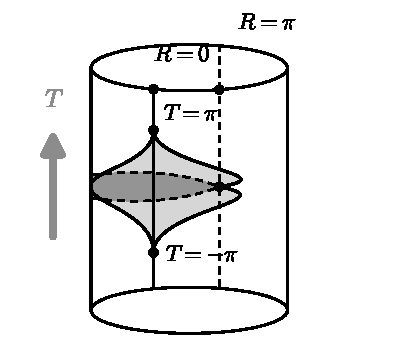
\includegraphics[width=0.72\textwidth]{fig_H.3.pdf}
\caption*{图 H.3\quad Einstein 静态宇宙 $\mathbf{R} \times S^{3}$，描绘成一个柱面。阴影区域与 Minkowski 空间共形相关。}
\end{figure}

事实上，Minkowski 空间只是上图（包括 $R = 0$ 在内）的\emph{内部}；边界并不属于原来的时空。这些边界被称为\textbf{共形无限远}（conformal infinity），而原时空与共形无限远之并集则称为\textbf{共形紧化}（conformal compactification），它是一个带边流形。共形图的结构使我们可以把共形无限远再细分成几个不同的区域：

\begin{figure}[H]
\centering
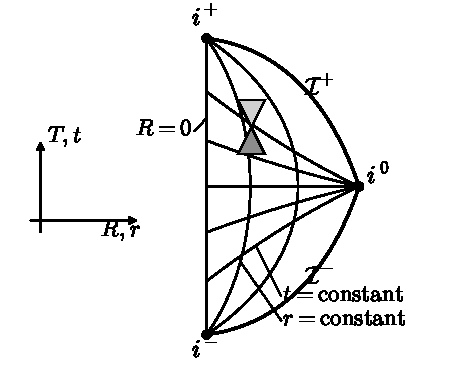
\includegraphics[width=0.72\textwidth]{fig_H.4.pdf}
\caption*{图 H.4\quad Minkowski 空间的共形图。整幅图中光锥都张成 $\pm 45^{\circ}$。}
\end{figure}

% ---- 书页 476 / p491 ----
\begin{equation*}
\begin{aligned}
i^{+} &= \text{未来类时无限远}\ (T=\pi,\ R=0)\\
i^{0} &= \text{类空无限远}\ (T=0,\ R=\pi)\\
i^{-} &= \text{过去类时无限远}\ (T=-\pi,\ R=0)\\
\mathscr{I}^{+} &= \text{未来类光无限远}\ (T=\pi-R,\ 0<R<\pi)\\
\mathscr{I}^{-} &= \text{过去类光无限远}\ (T=-\pi+R,\ 0<R<\pi)
\end{aligned}
\end{equation*}
（$\mathscr{I}^{+}$ 与 $\mathscr{I}^{-}$ 分别读作“scri-plus”与“scri-minus”。）注意，$i^{+}$、$i^{0}$ 与 $i^{-}$ 其实是\emph{点}，因为 $R = 0$ 与 $R = \pi$ 是 $S^{3}$ 的北极和南极。而 $\mathscr{I}^{+}$ 与 $\mathscr{I}^{-}$ 则实际上是类光曲面，具有 $\mathbf{R} \times S^{2}$ 的拓扑。

Minkowski 时空的共形图包含若干重要特征。图中径向类光测地线成 $\pm 45^{\circ}$。所有类时测地线都始于 $i^{-}$、终于 $i^{+}$；所有类光测地线都始于 $\mathscr{I}^{-}$、终于 $\mathscr{I}^{+}$；所有类空测地线则既始于 $i^{0}$ 又终于 $i^{0}$。另一方面，也可以存在终于类光无限远的非测地类时曲线，只要它们变得“渐近类光”。

能把整个 Minkowski 空间塞进一小张纸片上固然惬意，但其实我们并没有由此学到多少原来不知道的东西。共形图真正更有用武之地，是当我们想表示稍微复杂一些的时空的时候，比如黑洞的时空。如第 6 章所讨论的，渐近平直时空（或时空的一个区域）是指那些其 $\mathscr{I}^{+}$、$i^{0}$ 与 $\mathscr{I}^{-}$ 的结构与 Minkowski 空间相同的时空。同样重要的是，共形图让我们得以了解时空的因果结构，比如两个指定点的过去或未来光锥是否相交。在 Minkowski 空间中，任何两点都是如此；但弯曲时空可以更有趣，正如我们在第 2 章膨胀宇宙的例子中看到的那样。

让我们考虑第 2 章引入的那个宇宙学时空的共形图，它生动地展示了这一技术的用处。在空间上取极坐标后，度规变为
\begin{equation*}
ds^{2} = -\mathrm{d}t^{2} + t^{2q}\left(\mathrm{d}r^{2} + r^{2}d\Omega^{2}\right),
\tag{H.18}
\end{equation*}
其中我们对尺度因子选择了幂律行为 $a(t) = t^{q}$，且 $0 < q < 1$。这个度规与 Minkowski 空间度规的一个关键差别，在于 $t = 0$ 处存在奇点，它限制了坐标的取值范围：
\begin{equation*}
0 < t < \infty
\tag{H.19}
\end{equation*}
\begin{equation*}
0 \le r < \infty.
\tag{H.20}
\end{equation*}
除了这一受限制的坐标范围之外，我们的分析几乎完全照搬平直时空的情形。这是因为我们可以把度规式 (H.18) 化成平直时空乘以一个共形因子的形式；一旦做到这一点，我们只需重复之前的坐标变换，就能把膨胀宇宙的度规表达为 Einstein 静态宇宙的度规乘以一个共形因子。

% ---- 书页 477 / p492 ----
我们首先选取一个新的时间坐标 $\eta$，它有时被称为\textbf{共形时间}（conformal time），满足
\begin{equation*}
\mathrm{d}t^{2} = t^{2q}\mathrm{d}\eta^{2},
\tag{H.21}
\end{equation*}
亦即
\begin{equation*}
\eta = \frac{1}{1-q}\,t^{1-q}.
\tag{H.22}
\end{equation*}
这一简单选择让我们得以把尺度因子提取成一个整体共形因子：
\begin{equation*}
ds^{2} = \left[(1-q)\eta\right]^{2q/(1-q)}\left(-\mathrm{d}\eta^{2} + \mathrm{d}r^{2} + r^{2}d\Omega^{2}\right).
\tag{H.23}
\end{equation*}
$\eta$ 的取值范围与 $t$ 相同，
\begin{equation*}
0 < \eta < \infty.
\tag{H.24}
\end{equation*}
注意，$\eta$ 是一个类时坐标［意义是矢量 $\partial_{\eta}$ 是类时的，$ds^{2}(\partial_{\eta},\partial_{\eta}) < 0$］，但它并不量度共动时钟（空间坐标为常数的时钟）的固有时。如果我们考虑轨迹 $x^{\mu}(\lambda) = (\eta(\lambda), 0, 0, 0)$，并计算固有时 $\tau(\eta)$，就会发现它等于我们先前的那个时间坐标，而不是新的这个：$\tau \propto t \propto \eta^{1/(1-q)}$。所以 $\eta$ 是类时坐标，却不是任何人实际会测到的时间。这完全没有问题，恰好可以作为一个例证，说明可观测量与时空坐标这两个概念是彼此独立的。

既然膨胀宇宙的度规已经写成了共形因子乘 Minkowski 度规的形式，我们就可以施行同一串坐标变换——式 (H.5)、(H.8) 与 (H.13)——只不过让 $\eta$ 顶替 $t$ 的位置。这些变换把我们的坐标从 $(\eta, r)$ 变到 $(T, R)$，此时的取值范围为
\begin{equation*}
0 \le R, \qquad 0 < T, \qquad T + R < \pi.
\tag{H.25}
\end{equation*}
度规式 (H.23) 变为
\begin{equation*}
ds^{2} = \omega^{-2}(T,R)\left(-\mathrm{d}T^{2} + \mathrm{d}R^{2} + \sin^{2}R\,d\Omega^{2}\right),
\tag{H.26}
\end{equation*}
其中，经过对三角恒等式的一番英勇运用，可以发现共形因子形如
\begin{equation*}
\omega(T,R) = \left(\frac{\cos T + \cos R}{2\sin T}\right)^{2q}(\cos T + \cos R).
\tag{H.27}
\end{equation*}
共形因子的精确形状其实并非头等重要；关键的特征是，我们又一次把度规表达成了 Einstein 静态宇宙的度规乘以一个共形因子。这个情形与平直时空情形的重要区别在于，类时坐标终止于 $T = 0$ 处的奇点；除此之外，时空图完全相同。

% ---- 书页 478 / p493 ----
于是我们得到图 H.5 的共形图，它看上去像 Minkowski 图（图 H.4）的上半部分。光锥依旧张成 $45^{\circ}$。我们看到共形图如何让因果结构一目了然：很容易在时空中选出两个事件，使得它们的过去光锥在相交之前先撞上奇点（而未来光锥则总会交叠）。对于更复杂的几何，这种表示时空的便利方式将更加有用。

\begin{figure}[H]
\centering
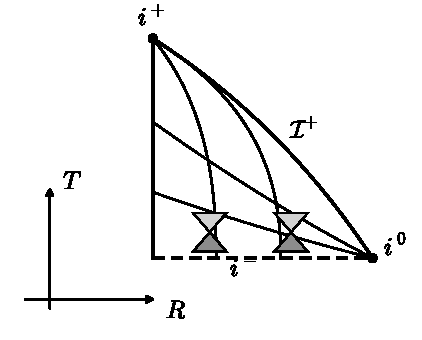
\includegraphics[width=0.72\textwidth]{fig_H.5.pdf}
\caption*{图 H.5\quad Robertson--Walker 宇宙（$a(t) \propto t^{q}$，$0<q<1$）的共形图。虚线代表 $t = 0$ 处的奇点（它同时对应于 $T = 0$）。}
\end{figure}

% 附录I The Parallel Propagator

\chapter{平行移动传播子}

沿一条曲线把一个张量平行移动的想法，显然在广义相对论中具有核心的重要性。对于一个沿路径 $x^\mu(\lambda)$ 被输运的矢量 $V^\mu$，平行移动方程为
\begin{equation*}
\frac{dx^\mu}{d\lambda}\nabla_\mu V^\nu \equiv \frac{dx^\mu}{d\lambda}\partial_\mu V^\nu + \frac{dx^\mu}{d\lambda}\Gamma^\nu_{\mu\sigma}V^\sigma = 0.
\tag{I.1}
\end{equation*}

结果表明，可以对这个方程写下一个显式而一般的解；这个解有些形式化，但无论是其本身，还是它同量子场论中一些技术的联系，都颇有意思。

我们首先注意到，对某条路径 $\gamma:\lambda\to x^\sigma(\lambda)$，求解矢量 $V^\mu$ 的平行移动方程就相当于寻找一个矩阵 $P^\mu{}_\rho(\lambda,\lambda_0)$，它把矢量的初始值 $V^\mu(\lambda_0)$ 与它沿路径稍后某处的值联系起来：
\begin{equation*}
V^\mu(\lambda) = P^\mu{}_\rho(\lambda,\lambda_0)V^\rho(\lambda_0).
\tag{I.2}
\end{equation*}

当然，这个被称为\textbf{平行移动传播子}（parallel propagator）的矩阵 $P^\mu{}_\rho(\lambda,\lambda_0)$ 依赖于路径 $\gamma$（尽管很难找到一种记号来表明这一点，而又不让 $\gamma$ 看起来像一个指标）。如果我们定义
\begin{equation*}
A^\mu{}_\rho(\lambda) = -\Gamma^\mu_{\sigma\rho}\frac{dx^\sigma}{d\lambda},
\tag{I.3}
\end{equation*}
其中右端的量在 $x^\nu(\lambda)$ 处取值，那么平行移动方程就变成
\begin{equation*}
\frac{d}{d\lambda}V^\mu = A^\mu{}_\rho V^\rho.
\tag{I.4}
\end{equation*}

由于平行移动传播子必须对任何矢量都适用，把式 (I.2) 代入式 (I.4) 可知，$P^\mu{}_\rho(\lambda,\lambda_0)$ 也服从这个方程：
\begin{equation*}
\frac{d}{d\lambda}P^\mu{}_\rho(\lambda,\lambda_0) = A^\mu{}_\sigma(\lambda)P^\sigma{}_\rho(\lambda,\lambda_0).
\tag{I.5}
\end{equation*}

为了求解这个方程，先对两边积分：
\begin{equation*}
P^\mu{}_\rho(\lambda,\lambda_0) = \delta^\mu_\rho + \int_{\lambda_0}^{\lambda} A^\mu{}_\sigma(\eta)P^\sigma{}_\rho(\eta,\lambda_0)\,d\eta.
\tag{I.6}
\end{equation*}

容易看出，Kronecker $\delta$ 符号（Kronecker delta）在 $\lambda=\lambda_0$ 时给出了正确的归一化。

我们可以用迭代法求解式 (I.6)：把右端代入它自身，如此反复，便得到
\begin{equation*}
P^\mu{}_\rho(\lambda,\lambda_0) = \delta^\mu_\rho + \int_{\lambda_0}^{\lambda} A^\mu{}_\rho(\eta)\,d\eta + \int_{\lambda_0}^{\lambda}\int_{\lambda_0}^{\eta} A^\mu{}_\sigma(\eta)A^\sigma{}_\rho(\eta')\,d\eta'\,d\eta + \cdots.
\tag{I.7}
\end{equation*}

这个级数中的第 $n$ 项是在一个 $n$ 维直角三角形——即 $n$ 维单纯形（$n$-simplex）——上的积分：
\begin{align*}
&\int_{\lambda_0}^{\lambda} A(\eta_1)\,d\eta_1 \\
&\int_{\lambda_0}^{\lambda}\int_{\lambda_0}^{\eta_2} A(\eta_2)A(\eta_1)\,d\eta_1 d\eta_2 \\
&\int_{\lambda_0}^{\lambda}\int_{\lambda_0}^{\eta_3}\int_{\lambda_0}^{\eta_2} A(\eta_3)A(\eta_2)A(\eta_1)\,d^3\eta.
\end{align*}
见图 I.1。

\begin{figure}[H]
\centering
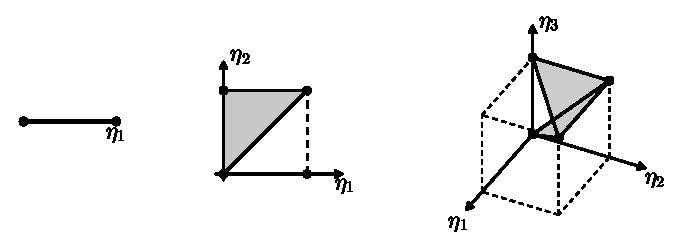
\includegraphics[width=0.72\textwidth]{fig_I.1.pdf}
\caption*{图 I.1\quad $n$ 维单纯形（$n$ 维直角三角形），$n = 1, 2, 3$。}
\end{figure}

如果我们能把这样的积分看成是在一个 $n$ 维立方体（$n$-cube）而不是 $n$ 维单纯形上进行，事情会简单一些。有没有办法做到这一点呢？每个立方体中有 $n!$ 个这样的单纯形，所以我们必须乘以 $1/n!$ 来补偿这块多出来的体积。但我们还想把被积函数也弄对；用矩阵记号，$n$ 阶的被积函数是 $A(\eta_n)A(\eta_{n-1})\cdots A(\eta_1)$，只是附带一个特殊性质：$\eta_n \ge \eta_{n-1} \ge \cdots \ge \eta_1$。因此我们定义\textbf{路径排序符号}（path-ordering symbol）$\mathcal{P}$，用它来保证这个条件成立。换句话说，表达式
\begin{equation*}
\mathcal{P}\left[A(\eta_n)A(\eta_{n-1})\cdots A(\eta_1)\right]
\tag{I.8}
\end{equation*}
代表这 $n$ 个矩阵 $A(\eta_i)$ 的乘积，其排序方式为：$\eta_i$ 值最大者排在最左边，其后每个 $\eta_i$ 的值都小于或等于前一个值。于是我们可以把式 (I.7) 中的 $n$ 阶项写成
\begin{align*}
&\int_{\lambda_0}^{\lambda}\int_{\lambda_0}^{\eta_n}\cdots\int_{\lambda_0}^{\eta_2} A(\eta_n)A(\eta_{n-1})\cdots A(\eta_1)\,d^n\eta \\
&\quad = \frac{1}{n!}\int_{\lambda_0}^{\lambda}\int_{\lambda_0}^{\lambda}\cdots\int_{\lambda_0}^{\lambda} \mathcal{P}\left[A(\eta_n)A(\eta_{n-1})\cdots A(\eta_1)\right] d^n\eta.
\tag{I.9}
\end{align*}

这个表达式对矩阵 $A(\eta_i)$ 没有给出任何实质性的陈述；它纯粹是一种记号。但现在我们可以把式 (I.7) 写成矩阵形式：
\begin{equation*}
P(\lambda,\lambda_0) = \mathbf{1} + \sum_{n=1}^{\infty} \frac{1}{n!}\int_{\lambda_0}^{\lambda} \mathcal{P}\left[A(\eta_n)A(\eta_{n-1})\cdots A(\eta_1)\right] d^n\eta.
\tag{I.10}
\end{equation*}

这个公式正是指数函数的级数表达式；因此我们说，平行移动传播子由路径排序指数（path-ordered exponential）给出
\begin{equation*}
P(\lambda,\lambda_0) = \mathcal{P}\exp\left(\int_{\lambda_0}^{\lambda} A(\eta)\,d\eta\right),
\tag{I.11}
\end{equation*}
这同样只是记号；路径排序指数就定义为式 (I.10) 的右端。我们可以把它写得更显式一些：
\begin{equation*}
\boxed{\,P^\mu{}_\nu(\lambda,\lambda_0) = \mathcal{P}\exp\left(-\int_{\lambda_0}^{\lambda} \Gamma^\mu_{\sigma\nu}\frac{dx^\sigma}{d\eta}\,d\eta\right).}
\tag{I.12}
\end{equation*}

能有一个显式公式总归是件好事，哪怕它相当抽象。同样类型的表达式也出现在量子场论中，即所谓的“Dyson 公式”（Dyson's Formula）；它之所以在那里出现，是因为时间演化算符的 Schrödinger 方程与式 (I.5) 具有相同的形式。

平行移动传播子一个特别有意思的例子出现在路径是一个回路（loop）——即从同一点出发、又终止于同一点——的情形。这时，如果联络是度规相容的，所得到的矩阵就恰好是切空间在该点处的一个洛伦兹变换。这个变换就是所谓的这条回路的“和乐”（holonomy）。如果你知道每一条可能回路的和乐，事实证明这等价于知道度规。于是人们可以在“圈表示”（loop representation）中考察广义相对论，其中基本变量是和乐而不是显式的度规。有一个名为“圈量子引力”（loop quantum gravity）的研究纲领，试图用这些变量直接把广义相对论量子化（有别于弦论那样的进路——在弦论中，GR 会在某个极限下自动出现）。在这个方向上已经取得了大量的数学进展，但根本性的障碍依然存在。\footnote{关于这一进路的综述，见 C.~Rovelli, “Loop quantum gravity,” \emph{Living Rev.~Rel.}~\textbf{1}, 1 (1998), \texttt{http://arxiv.org/gr-qc/9710008}。}

% 书页 482（p497）为空白页，无正文内容；附录 J 自书页 483 起，由另一块负责。

% 附录J Noncoordinate Bases

\chapter{非坐标基}

% ---- 书页 483 / p498 ----
在研究流形的早期，我们曾决定为切空间选取与坐标相适配的基。既出于审美也出于实用的理由，我们应当再一次考察联络与曲率的形式体系，但这一次在切空间中使用一组\emph{并非}取自任何坐标系的基矢量。将会看到，这一侧重点上的小小改变，会揭示出看待联络与曲率的另一种视角；在这种视角下，它与粒子物理中规范理论（gauge theories）的联系要透明得多。事实上，将要引入的概念非常直截了当，只是这套记号是一场噩梦，所以它看起来比实际上更难。

迄今为止，我们一直在利用这样一个事实：在点 $p$ 处，切空间 $T_{p}$ 的一个自然基由对该点坐标的偏导数给出，即 $\hat{e}_{(\mu)} = \partial_{\mu}$；类似地，余切空间 $T_{p}^{*}$ 的一个基由坐标函数的梯度给出，即 $\hat{\theta}^{(\mu)} = \mathrm{d}x^{\mu}$。然而，没有什么能阻止我们随自己的心意搭建任意的基。因此，让我们设想在流形的每一点引入一组基矢量 $\hat{e}_{(a)}$（用拉丁字母而非希腊字母作指标，以提醒我们它们不与任何坐标系相联系）。我们将把这些基矢量选成“正交归一的”（orthonormal），其含义与我们所工作的流形的号差相适配。也就是说，如果度规的规范形式写作 $\eta_{ab}$，我们就要求基矢量的内积为
\begin{equation*}
g(\hat{e}_{(a)}, \hat{e}_{(b)}) = \eta_{ab},
\tag{J.1}
\end{equation*}
其中 $g(\ ,\ )$ 是通常的度规张量。于是，在洛伦兹型时空中 $\eta_{ab}$ 代表 Minkowski 度规，而在具有正定度规的空间中它则代表欧几里得度规。构成正交归一基的这组矢量有时被称为一个 \textbf{tetrad}（即“四标架”，源自希腊语 tetras，“四个一组”）或 \textbf{vielbein}（源自德语，意为“许多条腿”）。在不同的维数下，它偶尔也被称为 \emph{vierbein}（四）、\emph{dreibein}（三）、\emph{zweibein}（二），等等。正如我们一般找不到覆盖整个流形的坐标卡片，我们也常常无法找到一组处处有定义的光滑基矢量场。照例，我们可以通过在不同的片（patch）上工作、并确保各片在交叠处表现良好来克服这个问题。

拥有一个基的意义在于：任何矢量都可以表示为基矢量的线性组合。具体地说，我们可以把原来的基矢量

% ---- 书页 484 / p499 ----
$\hat{e}_{(\mu)} = \partial_{\mu}$ 用新的基表示出来：
\begin{equation*}
\hat{e}_{(\mu)} = e_{\mu}{}^{a}\hat{e}_{(a)}.
\tag{J.2}
\end{equation*}
分量 $e_{\mu}{}^{a}$ 构成一个 $n\times n$ 的可逆矩阵。（按照我们通常把对象与其分量混为一谈的做法，我们将把 $e_{\mu}{}^{a}$ 称为 tetrad 或 vielbein，而且常用其复数形式“vielbeins”。）我们把指标换位来表示它们的逆，得到 $e^{\mu}{}_{a}$，它们满足
\begin{equation*}
e^{\mu}{}_{a}e_{\nu}{}^{a} = \delta^{\mu}_{\nu}, \qquad e_{\mu}{}^{a}e^{\mu}{}_{b} = \delta^{a}_{b}.
\tag{J.3}
\end{equation*}
它们正是矢量 $\hat{e}_{(a)}$ 在坐标基下的分量：
\begin{equation*}
\hat{e}_{(a)} = e^{\mu}{}_{a}\hat{e}_{(\mu)}.
\tag{J.4}
\end{equation*}
用逆 vielbein 表示，式 (J.1) 变为
\begin{equation*}
g_{\mu\nu}e^{\mu}{}_{a}e^{\nu}{}_{b} = \eta_{ab},
\tag{J.5}
\end{equation*}
或者等价地
\begin{equation*}
g_{\mu\nu} = e_{\mu}{}^{a}e_{\nu}{}^{b}\eta_{ab}.
\tag{J.6}
\end{equation*}
这最后一个方程有时使人们说，vielbein 是度规的“平方根”。

我们可以类似地在 $T_{p}$ 中搭建一组正交归一的 1-形式基，记作 $\hat{\theta}^{(a)}$。可以选取它们与基矢量相容，也就是说
\begin{equation*}
\hat{\theta}^{(a)}(\hat{e}_{(b)}) = \delta^{a}_{b}.
\tag{J.7}
\end{equation*}
一个直接的推论是：这组正交归一 1-形式与其基于坐标的表亲 $\hat{\theta}^{(\mu)} = \mathrm{d}x^{\mu}$ 之间的关系为
\begin{equation*}
\hat{\theta}^{(\mu)} = e^{\mu}{}_{a}\hat{\theta}^{(a)}
\tag{J.8}
\end{equation*}
以及
\begin{equation*}
\hat{\theta}^{(a)} = e_{\mu}{}^{a}\hat{\theta}^{(\mu)}.
\tag{J.9}
\end{equation*}
于是，vielbein $e_{\mu}{}^{a}$ 身兼二职：既是坐标基矢量用正交归一基矢量表出的分量，又是正交归一基 1-形式用坐标基 1-形式表出的分量；而逆 vielbein 则既是正交归一基矢量用坐标基表出的分量，又是坐标基 1-形式用正交归一基表出的分量。

% ---- 书页 485 / p500 ----
任何其他矢量也可以用它在正交归一基中的分量来表示。如果矢量 $V$ 在坐标基中写作 $V^{\mu}\hat{e}_{(\mu)}$，在正交归一基中写作 $V^{a}\hat{e}_{(a)}$，那么这两组分量之间的关系为
\begin{equation*}
V^{a} = e_{\mu}{}^{a}V^{\mu}.
\tag{J.10}
\end{equation*}
这样，vielbein 让我们可以“在拉丁指标和希腊指标之间来回切换”。张量的一个美妙性质——基于指标的位置，通常只有一种合理的做法——在这里帮了大忙。我们可以进一步用两种基中的任何一种来标记多指标张量，甚至用混合分量来标记：
\begin{equation*}
V^{a}{}_{b} = e_{\mu}{}^{a}V^{\mu}{}_{b} = e^{\nu}{}_{b}V^{a}{}_{\nu} = e_{\mu}{}^{a}e^{\nu}{}_{b}V^{\mu}{}_{\nu}.
\tag{J.11}
\end{equation*}
回头看式 (J.5)，我们看到度规张量在正交归一基中的分量恰好就是平直度规的分量 $\eta_{ab}$。（正因如此，希腊指标有时被称为“弯曲的”（curved），拉丁指标则被称为“平直的”（flat）。）事实上，我们甚至可以用平直度规及其逆 $\eta^{ab}$ 来升降拉丁指标。你可以自行验证一切都行之有效（例如，用度规降低指标的操作与在正交归一基和坐标基之间切换是相互对易的）。特别地，我们对逆 vielbein 的定义与我们通常的指标升降规则是一致的：
\begin{equation*}
e^{\mu}{}_{a} = g^{\mu\nu}\eta_{ab}e_{\nu}{}^{b}.
\tag{J.12}
\end{equation*}

我们引入 vielbein $e_{\nu}{}^{a}$ 时，是把它们当作一组基矢量在另一个基下求出的分量。这等价于把它们看作一个 $(1,1)$ 型张量的分量：
\begin{equation*}
e = e_{\nu}{}^{a}\mathrm{d}x^{\nu}\otimes\hat{e}_{(a)}.
\tag{J.13}
\end{equation*}
但这其实是一个我们早已熟知且喜爱的张量：恒等映射。让这个张量作用在一个矢量上，得到的仍是同一个矢量，只不过换了一个基；这正是式 (J.10) 的内容。同样，如果用逆 vielbein $e^{\mu}{}_{a}$ 把 $e_{\nu}{}^{a}$ 上的拉丁指标换成希腊指标，根据式 (J.3) 就得到 Kronecker delta $\delta^{\mu}_{\nu}$，它当然就是作用在矢量（或 1-形式）上的恒等映射。这一点值得强调，因为我们也可以选择把 $e_{\nu}{}^{a}$ 解释为一组矢量分量（有些参考文献正是这么做的），那样的话协变导数的形式会有所不同。引入了一组新的基矢量和 1-形式之后，我们便不得不重提我们最爱讨论的话题：变换性质。一直以来我们都小心强调，张量变换律只是坐标变换的间接结果；真正的问题在于基的改变。如今我们有了非坐标基，这些基就可以独立于坐标而改变。唯一的限制是必须保持正交归一性条件 (J.1)。但我们知道什么样的变换保持平直度规——在欧几里得号差的度规下它们是正交变

% ---- 书页 486 / p501 ----
换，而在洛伦兹号差的度规下则是洛伦兹变换。因此我们考虑如下形式的基变换：
\begin{equation*}
\hat{e}_{(a)} \to \hat{e}_{(a')} = \Lambda^{a}{}_{a'}(x)\hat{e}_{(a)},
\tag{J.14}
\end{equation*}
其中矩阵 $\Lambda^{a}{}_{a'}(x)$ 表示依赖于位置的变换，它们（在每一点）保持度规的规范形式不变：
\begin{equation*}
\Lambda^{a}{}_{a'}\Lambda^{b}{}_{b'}\eta_{ab} = \eta_{a'b'}.
\tag{J.15}
\end{equation*}
事实上，这些矩阵对应于我们在平直空间中所说的逆洛伦兹变换（作用在基矢量上的那类）；与之前一样，我们也有普通的洛伦兹变换 $\Lambda^{a'}{}_{a}$，它变换基 1-形式。就分量而言，与之前一样，我们用 $\Lambda^{a'}{}_{a}$ 变换上指标，用 $\Lambda^{a}{}_{a'}$ 变换下指标。

于是，我们现在获得了在空间的每一点都实施一个洛伦兹变换的自由（视号差而定，也可以是普通的欧几里得转动）。这些变换因此被称为\textbf{局部洛伦兹变换}（local Lorentz transformations），简称 LLT。我们仍然保有通常的改变坐标的自由，这被称为\textbf{广义坐标变换}（general coordinate transformations），简称 GCT。两者可以同时发生，由此得到一个混合的张量变换律：
\begin{equation*}
T^{a'\mu'}{}_{b'\nu'} = \Lambda^{a'}{}_{a}\frac{\partial x^{\mu'}}{\partial x^{\mu}}\Lambda^{b}{}_{b'}\frac{\partial x^{\nu}}{\partial x^{\nu'}}T^{a\mu}{}_{b\nu}.
\tag{J.16}
\end{equation*}
把我们关于张量的知识翻译成非坐标基的语言，在多数情况下只不过是把 vielbein 塞到正确的位置而已。关键的例外出现在我们要对东西求导的时候。在我们通常的形式体系中，张量的协变导数等于它的偏导数再加上若干修正项——每个指标一项——涉及该张量与联络系数。同样的程序对非坐标基依然成立，只是要把通常的联络系数 $\Gamma^{\lambda}_{\mu\nu}$ 换成\textbf{自旋联络}（spin connection），记作 $\omega_{\mu}{}^{a}{}_{b}$。每个拉丁指标都以通常的方式配上一项自旋联络：
\begin{equation*}
\nabla_{\mu}X^{a}{}_{b} = \partial_{\mu}X^{a}{}_{b} + \omega_{\mu}{}^{a}{}_{c}X^{c}{}_{b} - \omega_{\mu}{}^{c}{}_{b}X^{a}{}_{c}.
\tag{J.17}
\end{equation*}
（“自旋联络”这个名字源于这样一个事实：可以用它来对旋量求协变导数，而用常规的联络系数这实际上是做不到的。）当拉丁指标和希腊指标混合出现时，我们会同时得到两种类型的项。

张量应当与其写法无关这一通常要求，让我们得以推导自旋联络、vielbein 与 $\Gamma^{\lambda}_{\mu\nu}$ 之间的关系。考虑矢量 $X$ 的协变导数，先在纯坐标基中：
\begin{align*}
\nabla X &= (\nabla_{\mu}X^{\nu})\mathrm{d}x^{\mu}\otimes\partial_{\nu} \\
&= (\partial_{\mu}X^{\nu} + \Gamma^{\nu}_{\mu\lambda}X^{\lambda})\mathrm{d}x^{\mu}\otimes\partial_{\nu}. \tag{J.18}
\end{align*}

% ---- 书页 487 / p502 ----
现在在混合基中求同一个对象，再转换到坐标基：
\begin{align*}
\nabla X &= (\nabla_{\mu}X^{a})\mathrm{d}x^{\mu}\otimes\hat{e}_{(a)} \\
&= (\partial_{\mu}X^{a} + \omega_{\mu}{}^{a}{}_{b}X^{b})\mathrm{d}x^{\mu}\otimes\hat{e}_{(a)} \\
&= \big(\partial_{\mu}(e_{\nu}{}^{a}X^{\nu}) + \omega_{\mu}{}^{a}{}_{b}e_{\lambda}{}^{b}X^{\lambda}\big)\mathrm{d}x^{\mu}\otimes(e^{\sigma}{}_{a}\partial_{\sigma}) \\
&= e^{\sigma}{}_{a}\big(e_{\nu}{}^{a}\partial_{\mu}X^{\nu} + X^{\nu}\partial_{\mu}e_{\nu}{}^{a} + \omega_{\mu}{}^{a}{}_{b}e_{\lambda}{}^{b}X^{\lambda}\big)\mathrm{d}x^{\mu}\otimes\partial_{\sigma} \\
&= \big(\partial_{\mu}X^{\nu} + e^{\nu}{}_{a}\partial_{\mu}e_{\lambda}{}^{a}X^{\lambda} + e^{\nu}{}_{a}e_{\lambda}{}^{b}\omega_{\mu}{}^{a}{}_{b}X^{\lambda}\big)\mathrm{d}x^{\mu}\otimes\partial_{\nu}. \tag{J.19}
\end{align*}
与式 (J.18) 比较可得
\begin{equation*}
\Gamma^{\nu}_{\mu\lambda} = e^{\nu}{}_{a}\partial_{\mu}e_{\lambda}{}^{a} + e^{\nu}{}_{a}e_{\lambda}{}^{b}\omega_{\mu}{}^{a}{}_{b},
\tag{J.20}
\end{equation*}
或者等价地
\begin{equation*}
\omega_{\mu}{}^{a}{}_{b} = e_{\nu}{}^{a}e^{\lambda}{}_{b}\Gamma^{\nu}_{\mu\lambda} - e^{\lambda}{}_{b}\partial_{\mu}e_{\lambda}{}^{a}.
\tag{J.21}
\end{equation*}
稍作处理，就可以把这个关系写成 vielbein 的协变导数为零：
\begin{align*}
\nabla_{\mu}e_{\nu}{}^{a} &= \partial_{\mu}e_{\nu}{}^{a} - \Gamma^{\lambda}_{\mu\nu}e_{\lambda}{}^{a} + \omega_{\mu}{}^{a}{}_{b}e_{\nu}{}^{b} \\
&= 0, \tag{J.22}
\end{align*}
它有时被称为“tetrad 假设”（tetrad postulate）。注意，它总是成立的；推导它并不需要对联络作任何假设。具体地说，我们不需要假设联络是度规相容的或无挠的。不过，我们确实隐含地取 $e_{\nu}{}^{a}$ 代表 $(1,1)$ 型张量 (J.13)；既然这个张量就是恒等映射，它的协变导数为零也就不足为奇了。（并非所有文献都持这种观点，所以要当心。）

既然联络可以被看作我们为修补协变导数的变换律而不得不引入的东西，那么自旋联络本身不服从张量变换律也就不足为怪了。实际上，在 GCT 之下，那个下希腊指标确实按正确的方式变换，即像 1-形式那样。但在 LLT 之下，自旋联络非齐次地变换：
\begin{equation*}
\omega_{\mu}{}^{a'}{}_{b'} = \Lambda^{a'}{}_{a}\Lambda^{b}{}_{b'}\omega_{\mu}{}^{a}{}_{b} - \Lambda^{c}{}_{b'}\partial_{\mu}\Lambda^{a'}{}_{c}.
\tag{J.23}
\end{equation*}
建议你自行验证，这确实能使协变导数按正确的方式变换。

到目前为止，我们做的不过是空洞的形式主义——把已经知道的东西翻译成一套新记号。但我们做的这些工作确实换来了两样东西。第一样我们已经提到过：能够描述时空上的旋量场并对它们求协变导数；这里我们不再深入。第二样是视角的改变：我们可以把各种张量看作张量值的微分形式（tensor-valued differential forms）。例如，像 $X_{\mu}{}^{a}$ 这样的对象——我们

% ---- 书页 488 / p503 ----
把它看作带混合指标的 $(1,1)$ 型张量——也可以看作一个“矢量值的 1-形式”（vector-valued one-form）。它有一个下希腊指标，所以我们把它当作 1-形式，但对下指标的每一个取值它又是一个矢量。类似地，张量 $A_{\mu\nu}{}^{a}{}_{b}$（在 $\mu$ 和 $\nu$ 上反对称）可以看作一个“(1,1) 型张量值的 2-形式”。于是，任何带有若干个反对称下希腊指标和若干个拉丁指标的张量，都可以看作一个微分形式，只是取值于张量丛。（普通的微分形式简单来说就是标量值的形式。）当我们考虑外微分时，这一视角的用处就显现出来。如果我们想把 $X_{\mu}{}^{a}$ 当作矢量值的 1-形式，我们自然会想取它的外微分：
\begin{equation*}
(\mathrm{d}X)_{\mu\nu}{}^{a} = \partial_{\mu}X_{\nu}{}^{a} - \partial_{\nu}X_{\mu}{}^{a}.
\tag{J.24}
\end{equation*}
容易验证，这个对象在 GCT 之下像 2-形式一样变换［也就是说，按照 $(0,2)$ 型张量的变换律］，但在 LLT 之下却不像矢量那样变换（洛伦兹变换依赖于位置，这会在变换律中引入一个非齐次项）。不过，我们可以明智地运用自旋联络来修复这一点；由于非张量性的变换律 (J.23)，自旋联络可以被看作一个 1-形式，却不是张量值的 1-形式。于是，对象
\begin{equation*}
(\mathrm{d}X)_{\mu\nu}{}^{a} + (\omega\wedge X)_{\mu\nu}{}^{a} = \partial_{\mu}X_{\nu}{}^{a} - \partial_{\nu}X_{\mu}{}^{a} + \omega_{\mu}{}^{a}{}_{b}X_{\nu}{}^{b} - \omega_{\nu}{}^{a}{}_{b}X_{\mu}{}^{b},
\tag{J.25}
\end{equation*}
你可以自行验证，它会像一个正规的张量那样变换。

这套形式体系的一个直接应用是挠率和曲率的表达式——它们是刻画任何给定联络的两个张量。挠率带有两个反对称下指标，可以看作矢量值的 2-形式 $T_{\mu\nu}{}^{a}$。曲率总是在最后两个指标上反对称，是 $(1,1)$ 型张量值的 2-形式 $R^{a}{}_{b\mu\nu}$。利用我们在微分形式上省略指标的自由，可以用基 1-形式把它们表达为
\begin{equation*}
e^{a} = e_{\mu}{}^{a}\mathrm{d}x^{\mu}
\tag{J.26}
\end{equation*}
以及自旋联络 1-形式
\begin{equation*}
\omega^{a}{}_{b} = \omega_{\mu}{}^{a}{}_{b}\mathrm{d}x^{\mu}.
\tag{J.27}
\end{equation*}
注意我们已经更换了记号，定义 $e^{a} \equiv \hat{\theta}^{(a)}$。这是相当惯用的做法，而且更简洁。于是挠率和曲率的定义关系就是
\begin{equation*}
T^{a} = \mathrm{d}e^{a} + \omega^{a}{}_{b}\wedge e^{b}
\tag{J.28}
\end{equation*}
以及
\begin{equation*}
R^{a}{}_{b} = \mathrm{d}\omega^{a}{}_{b} + \omega^{a}{}_{c}\wedge\omega^{c}{}_{b}.
\tag{J.29}
\end{equation*}

% ---- 书页 489 / p504 ----
请记住，$R^{a}{}_{b}$ 代表整个 Riemann 张量（希腊指标被省略了）；不要把它与 Ricci 张量混淆。这两个式子就是所谓的 \textbf{Cartan 结构方程}（Cartan structure equations）。它们与通常的定义等价；让我们就挠率作一番证明练习，曲率的验证留给你自己完成。我们有
\begin{align*}
T_{\mu\nu}{}^{\lambda} &= e^{\lambda}{}_{a}T_{\mu\nu}{}^{a} \\
&= e^{\lambda}{}_{a}\big(\partial_{\mu}e_{\nu}{}^{a} - \partial_{\nu}e_{\mu}{}^{a} + \omega_{\mu}{}^{a}{}_{b}e_{\nu}{}^{b} - \omega_{\nu}{}^{a}{}_{b}e_{\mu}{}^{b}\big) \\
&= \Gamma^{\lambda}_{\mu\nu} - \Gamma^{\lambda}_{\nu\mu}, \tag{J.30}
\end{align*}
这正是我们最初给出的定义。这里我们用到了式 (J.20)，即用 vielbein 和自旋联络表出的 $\Gamma^{\lambda}_{\mu\nu}$。我们还可以把这些张量所满足的恒等式表达为
\begin{equation*}
\mathrm{d}T^{a} + \omega^{a}{}_{b}\wedge T^{b} = R^{a}{}_{b}\wedge e^{b}
\tag{J.31}
\end{equation*}
以及
\begin{equation*}
\mathrm{d}R^{a}{}_{b} + \omega^{a}{}_{c}\wedge R^{c}{}_{b} - R^{a}{}_{c}\wedge\omega^{c}{}_{b} = 0.
\tag{J.32}
\end{equation*}
其中第一式是 $R^{\rho}{}_{[\sigma\mu\nu]} = 0$ 的推广，第二式则是 Bianchi 恒等式 $\nabla_{[\lambda}R^{\rho}{}_{|\sigma|\mu\nu]} = 0$。（有时这两个方程都被称作 Bianchi 恒等式。）

这些表达式的形式会诱使人几乎无法抗拒地去定义一个“协变外微分”（covariant-exterior derivative）：它作用在张量值形式上，先取通常的外微分，再添上带自旋联络的适当项——每个拉丁指标一项。虽然这里我们不打算这样做，但向这种诱惑屈服也无妨；事实上，式 (J.28) 的右边以及式 (J.31) 和式 (J.32) 的左边，正可以看作这样的协变外微分。但要小心，式 (J.29) 却不能这样看；你不能对自旋联络取任何一种协变导数，因为它不是张量。

到目前为止，我们的方程对一般联络都成立；现在看看对 Christoffel 联络会得到什么。无挠要求就是 (J.28) 为零；这并不会直接给出关于自旋联络系数的任何简单表述。度规相容性则表现为度规的协变导数为零：$\nabla g = 0$。当我们把度规用正交归一基表达——此时它的分量就是简单的 $\eta_{ab}$——就能看到这会导出什么：
\begin{align*}
\nabla_{\mu}\eta_{ab} &= \partial_{\mu}\eta_{ab} - \omega_{\mu}{}^{c}{}_{a}\eta_{cb} - \omega_{\mu}{}^{c}{}_{b}\eta_{ac} \\
&= -\omega_{\mu ab} - \omega_{\mu ba}. \tag{J.33}
\end{align*}
于是令它等于零就意味着
\begin{equation*}
\omega_{\mu ab} = -\omega_{\mu ba}.
\tag{J.34}
\end{equation*}

% ---- 书页 490 / p505 ----
这样，度规相容性就等价于自旋联络在其拉丁指标上的反对称性。（和之前一样，只有当两个指标都在上或都在下时，这种说法才有意义。）这两个条件合在一起，让我们可以把自旋联络用 vielbein 表达出来。这个解有一个显式公式，但实践中更容易的做法是直接求解无挠条件
\begin{equation*}
\omega^{a}{}_{b}\wedge e^{b} = -\mathrm{d}e^{a},
\tag{J.35}
\end{equation*}
再利用自旋联络的非对称性求出各个分量。

思考非坐标基的最好理由之一是：在某些情形——包括计算曲率张量——它们确实能带来巨大的简化。让我们通过一个简单例子看看这是如何运作的：一个空间平直的膨胀宇宙，其度规为
\begin{equation*}
ds^{2} = -\mathrm{d}t^{2} + a^{2}(t)\delta_{ij}\mathrm{d}x^{i}\mathrm{d}x^{j}.
\tag{J.36}
\end{equation*}
我们将使用式 (J.26) 和式 (J.27) 的微分形式记号；像这样的计算就是很好的证据，说明这套语言不仅优雅而且确实实用。于是度规可以写成（对任何几何都成立）
\begin{equation*}
ds^{2} = \eta_{ab}e^{a}\otimes e^{b}.
\tag{J.37}
\end{equation*}
我们需要选取基 1-形式 $e^{a}$，使得上式与我们的度规 (J.36) 相吻合。有多种选择（它们由局部洛伦兹变换相联系），但其中有一个是显而易见的：
\begin{align*}
e^{0} &= \mathrm{d}t \\
e^{i} &= a\,\mathrm{d}x^{i}. \tag{J.38}
\end{align*}
现在我们想利用式 (J.35) 解出自旋联络。好消息是，基本上靠猜测就能做到。首先，适当地升降指标（用 $\eta^{ab}$ 和 $\eta_{ab}$），我们导出 $\omega_{ab}$ 反对称性的推论：
\begin{align*}
\omega^{0}{}_{0} &= 0 \\
\omega^{0}{}_{j} &= \omega^{j}{}_{0} \\
\omega^{i}{}_{j} &= -\omega^{j}{}_{i}. \tag{J.39}
\end{align*}
接下来计算式 (J.35) 的右边：
\begin{align*}
\mathrm{d}e^{0} &= 0 \\
\mathrm{d}e^{i} &= \mathrm{d}a\wedge\mathrm{d}x^{i} = \dot{a}\,\mathrm{d}t\wedge\mathrm{d}x^{i}, \tag{J.40}
\end{align*}

% ---- 书页 491 / p506 ----
然后再看左边：
\begin{align*}
\omega^{0}{}_{b}\wedge e^{b} &= \omega^{0}{}_{j}\wedge e^{j} = a\,\omega^{0}{}_{j}\wedge\mathrm{d}x^{j} \\
\omega^{i}{}_{b}\wedge e^{b} &= \omega^{i}{}_{0}\wedge e^{0} + \omega^{i}{}_{j}\wedge e^{j} = \omega^{i}{}_{0}\wedge\mathrm{d}t + \omega^{i}{}_{j}\wedge\mathrm{d}x^{j}. \tag{J.41}
\end{align*}
代入式 (J.35) 得到
\begin{align*}
\omega^{0}{}_{j}\wedge\mathrm{d}x^{j} &= 0 \\
\omega^{i}{}_{0}\wedge\mathrm{d}t + \omega^{i}{}_{j}\wedge\mathrm{d}x^{j} &= -\dot{a}\,\mathrm{d}t\wedge\mathrm{d}x^{i}. \tag{J.42}
\end{align*}
我们想从这些方程解出 $\omega^{a}{}_{b}$。很容易想到猜 $\omega^{0}{}_{j} = 0$；但这样一来，为了解第二个方程就需要 $\omega^{i}{}_{j} = -\dot{a}\delta^{i}_{j}\mathrm{d}t$，这与式 (J.39) 中的 $\omega^{i}{}_{j} = -\omega^{j}{}_{i}$ 不相容。不过，考虑到楔积的反对称性，我们可以令 $\omega^{0}{}_{j}$ 正比于 $\mathrm{d}x^{j}$ 来解第一个方程。确实，如果选取
\begin{equation*}
\omega^{0}{}_{j} = \dot{a}\,\mathrm{d}x^{j}, \qquad \omega^{i}{}_{0} = \dot{a}\,\mathrm{d}x^{i},
\tag{J.43}
\end{equation*}
就会发现，只要令
\begin{equation*}
\omega^{i}{}_{j} = 0.
\tag{J.44}
\end{equation*}
式 (J.42) 中的两个方程便都得到满足。

既然已经知道自旋联络，我们就能通过下式轻松得到曲率：
\begin{equation*}
R^{a}{}_{b} = \mathrm{d}\omega^{a}{}_{b} + \omega^{a}{}_{c}\wedge\omega^{c}{}_{b}.
\tag{J.45}
\end{equation*}
我们先计算自旋联络形式的外微分：
\begin{align*}
\mathrm{d}\omega^{i}{}_{0} &= \ddot{a}\,\mathrm{d}t\wedge\mathrm{d}x^{i} \\
\mathrm{d}\omega^{0}{}_{j} &= \ddot{a}\,\mathrm{d}t\wedge\mathrm{d}x^{j} \\
\mathrm{d}\omega^{i}{}_{j} &= 0, \tag{J.46}
\end{align*}
然后计算楔积：
\begin{align*}
\omega^{0}{}_{c}\wedge\omega^{c}{}_{0} &= 0 \\
\omega^{i}{}_{c}\wedge\omega^{c}{}_{0} &= 0 \\
\omega^{i}{}_{c}\wedge\omega^{c}{}_{j} &= \dot{a}^{2}\mathrm{d}x^{i}\wedge\mathrm{d}x^{j}. \tag{J.47}
\end{align*}
于是我们得到曲率 2-形式：
\begin{align*}
R^{0}{}_{0} &= 0 \\
R^{0}{}_{j} &= \ddot{a}\,\mathrm{d}t\wedge\mathrm{d}x^{j} \\
R^{i}{}_{0} &= \ddot{a}\,\mathrm{d}t\wedge\mathrm{d}x^{i} \\
R^{i}{}_{j} &= \dot{a}^{2}\mathrm{d}x^{i}\wedge\mathrm{d}x^{j}. \tag{J.48}
\end{align*}

% ---- 书页 492 / p507 ----
为了便于比较，我们可以用 vielbein 把 $R^{a}{}_{b\mu\nu}$ 换算成我们惯用的表达式 $R^{\rho}{}_{\sigma\mu\nu}$：
\begin{equation*}
R^{\rho}{}_{\sigma\mu\nu} = e^{\rho}{}_{a}e_{\sigma}{}^{b}R^{a}{}_{b\mu\nu}.
\tag{J.49}
\end{equation*}
用分量形式写出，vielbein (J.38) 及其逆为
\begin{equation*}
e_{\mu}{}^{a} = \begin{pmatrix} 1 & & & \\ & a & & \\ & & a & \\ & & & a \end{pmatrix}, \qquad e^{\nu}{}_{b} = \begin{pmatrix} 1 & & & \\ & a^{-1} & & \\ & & a^{-1} & \\ & & & a^{-1} \end{pmatrix}. \tag{J.50}
\end{equation*}
我们还需要计算基形式的楔积的分量，这相当直接：
\begin{equation*}
(\mathrm{d}x^{\alpha}\wedge\mathrm{d}x^{\beta})_{\mu\nu} = \delta^{\alpha}_{\mu}\delta^{\beta}_{\nu} - \delta^{\alpha}_{\nu}\delta^{\beta}_{\mu}.
\tag{J.51}
\end{equation*}
把所有这些放在一起，就得到 $R^{\rho}{}_{\sigma\mu\nu}$ 的分量：
\begin{align*}
R^{0}{}_{j0l} &= a\ddot{a}\delta_{jl} \\
R^{i}{}_{0k0} &= -\frac{\ddot{a}}{a}\delta^{i}_{k} \\
R^{i}{}_{jkl} &= \dot{a}^{2}(\delta^{i}_{k}\delta_{jl} - \delta^{i}_{l}\delta_{jk}), \tag{J.52}
\end{align*}
以及在最后两个指标上作反对称得到的那些分量。我们可以缩并，得到 Ricci 张量 $R_{\sigma\nu} = R^{\lambda}{}_{\sigma\lambda\nu}$ 的分量：
\begin{align*}
R_{00} &= -3\frac{\ddot{a}}{a} \\
R_{i0} &= 0 \\
R_{ij} &= (a\ddot{a} + 2\dot{a}^{2})\delta_{ij}. \tag{J.53}
\end{align*}
你可以验证，这与我们在第 8 章得到的结果一致。仅在这个简单的例子里，tetrad 方法在计算上就已经比坐标基方法简单；对于更复杂的度规，这种相对优势还会继续扩大。

借助于非坐标基的语言，我们可以把黎曼几何中联络与曲率的形式体系，同粒子物理中规范理论的形式体系加以比较。在这两种情形下，我们感兴趣的场都生活在指派给时空每一点的矢量空间里。在黎曼几何中，这些矢量空间包括切空间、余切空间以及由它们构造的高阶张量空间。而在规范理论中，我们关心的是“内部”矢量空间。区别在于：切空间及其同类与流形本身紧密相连，一旦流形被搭建起来，它们便自然地得到定义；例如，切空间可以看作一点处方向导数的空间。与此相反，内部矢量

% ---- 书页 493 / p508 ----
空间则可以有我们想要的任何维数，并且必须作为流形之外的一种独立添加来定义。用数学行话说，底流形与内部矢量空间（在每一点定义）的并就是一个\textbf{纤维丛}（fiber bundle），而矢量空间的每一份拷贝都被称为一根“纤维”（fiber）（与我们定义切丛的方式一致）。

除了底流形（对我们而言就是时空）和纤维之外，纤维丛定义中的另一个重要要素是“结构群”（structure group）：一个作用在纤维上的李群，它描述各纤维在相互交叠的坐标片上如何被缝合在一起。不深入细节地说，四维时空中切丛的结构群一般是 $\mathrm{GL}(4,\mathbf{R})$，即实可逆 $4\times4$ 矩阵群；如果有洛伦兹型度规，它可以约化为洛伦兹群 $SO(3,1)$。现在设想我们引入一个内部三维矢量空间，并用普通的转动把纤维缝合起来；这个新丛的结构群便是 $SO(3)$。生活在该丛中的场可以记作 $\phi^{A}(x^{\mu})$，其中 $A$ 从一取到三；它在流形的每一点上都是一个三维矢量（内部的，与时空无关）。我们可以随意选择纤维中的基；这意味着“物理量”应当在如下形式的局部 $SO(3)$ 变换下保持不变：
\begin{equation*}
\phi^{A}(x^{\mu}) \to \phi^{A'}(x^{\mu}) = O^{A'}{}_{A}(x^{\mu})\phi^{A}(x^{\mu}),
\tag{J.54}
\end{equation*}
其中 $O^{A'}{}_{A}(x^{\mu})$ 是 $SO(3)$ 中一个依赖于时空的矩阵。这类变换被称为\textbf{规范变换}（gauge transformations），在其下不变的理论被称为“规范理论”（gauge theories）。

在多数情况下，不难把事情安排得让物理量在规范变换下不变。唯一的困难出现在我们考虑偏导数 $\partial_{\mu}\phi^{A}$ 的时候。由于矩阵 $O^{A'}{}_{A}(x^{\mu})$ 依赖于时空，它会给偏导数的变换贡献一个不想要的项。到现在你应该已经能猜到解决方案了：引入一个联络，来修正变换律中的非齐次项。于是，我们把纤维丛上的联络定义为对象 $A_{\mu}{}^{A}{}_{B}$：它带两个“群指标”和一个时空指标。在 GCT 之下它像 1-形式那样变换，而在规范变换之下它的变换律是
\begin{equation*}
A_{\mu}{}^{A'}{}_{B'} = O^{A'}{}_{A}O^{B}{}_{B'}A_{\mu}{}^{A}{}_{B} - O^{C}{}_{B'}\partial_{\mu}O^{A'}{}_{C}.
\tag{J.55}
\end{equation*}
（当心：我们的约定与粒子物理文献中的约定不同。）在这个变换律下，“规范协变导数”（gauge covariant derivative）
\begin{equation*}
D_{\mu}\phi^{A} = \partial_{\mu}\phi^{A} + A_{\mu}{}^{A}{}_{B}\phi^{B}
\tag{J.56}
\end{equation*}
在规范变换下“像张量那样”变换，欢迎你自行验证。［在普通的电磁学中，联络就是惯用的矢势。不需要任何指标，因为结构群 $U(1)$ 是一维的。］

% ---- 书页 494 / p509 ----
显然，内部纤维丛上联络的这一概念，与切丛上的联络密切相关，尤其是在我们一直讨论的正交归一标架图像中。例如，变换律 (J.55) 就与自旋联络的变换律 (J.23) 完全相同。我们还可以定义一个曲率张量，或称“场强”（field strength）张量，它是一个 2-形式：
\begin{equation*}
F^{A}{}_{B} = \mathrm{d}A^{A}{}_{B} + A^{A}{}_{C}\wedge A^{C}{}_{B},
\tag{J.57}
\end{equation*}
与式 (J.29) 完全对应。我们可以沿路径平行移动物体，也有一个与平行移动传播子类似的结构；把一个矢量沿闭合曲线平行移动一周，所得矩阵的迹被称为“Wilson 圈”（Wilson loop）。

我们本可以继续发展切丛与内部矢量丛之间的关系，但那就得另写一本书了。让我们转而通过强调这两种构造之间的重要\emph{差异}来收尾。差异源于这样一个事实：切丛与底流形紧密相关，而其他纤维丛则是事后才附加上去的。说 $p$ 点切空间中的一个矢量“指向沿一条穿过 $p$ 的路径的方向”是有意义的；但对内部矢量丛来说，这种说法毫无意义。因此，内部空间没有坐标基的类似物——沿曲线的偏导数与内部矢量毫无关系。依次推下去，也就没有类似 vielbein 那样把正交归一基与坐标基联系起来的东西。特别是挠率张量，只对切丛上的联络才有定义，对任何规范理论联络都没有；它可以被看作 vielbein 的协变外微分，而内部丛上没有这样的构造。你应当领会联络这一概念的不同用法之间的联系，但同时也别忘乎所以。

\section{习题}

% 习题编号照原书
\textbf{1.}\quad 在式 (J.37) 中我们提过，度规在正交归一基中可以写成
\begin{equation*}
ds^{2} = \eta_{ab}e^{a}\otimes e^{b}.
\tag{J.58}
\end{equation*}
这怎么可能呢？如果度规的分量处处都是 $\eta_{ab}$，我们怎么可能知道几何是什么？

\textbf{2.}\quad 计算 Mixmaster 宇宙（Mixmaster universe）的联络 1-形式、曲率 2-形式，进而求出 Riemann 张量的分量。度规为
\begin{equation*}
ds^{2} = -\mathrm{d}t\otimes\mathrm{d}t + \alpha^{2}\sigma^{1}\otimes\sigma^{1} + \beta^{2}\sigma^{2}\otimes\sigma^{2} + \gamma^{2}\sigma^{3}\otimes\sigma^{3}.
\end{equation*}
其中 $\alpha$、$\beta$、$\gamma$ 只是 $t$ 的函数，而 1-形式 $\sigma^{i}$ 为
\begin{align*}
\sigma^{1} &= \cos\psi\,\mathrm{d}\theta + \sin\psi\sin\theta\,\mathrm{d}\phi \\
\sigma^{2} &= \sin\psi\,\mathrm{d}\theta - \cos\psi\sin\theta\,\mathrm{d}\phi \\
\sigma^{3} &= \mathrm{d}\psi + \cos\theta\,\mathrm{d}\phi.
\end{align*}


 % 本文件由 scripts/assemble.py 自动装配，勿手改（改 parts/ 后重跑）
% 文献目录

\chapter*{文献目录}
\markboth{文献目录}{}
\addcontentsline{toc}{chapter}{文献目录}

在正文中，我没有尝试为原始文献提供细致的引用。本着聚焦教学的原则，我在适当的地方给出了近期综述文章的参考文献。这里我列出若干书籍，它们或许可以作为你手中这本书的有用补充；这份清单无意做到包罗无遗，而是聚焦于那些仍在印行、且恰好为我所熟悉的书。

有两个网站是跟踪引力物理最新工作的宝贵资源。第一个是面向广义相对论与量子宇宙学的 ArXiv 电子预印本服务器：

\begin{center}
\texttt{http://arxiv.org/form/gr-qc/}
\end{center}

世界各地的研究者把他们最新的论文放在这里，随后便可以方便地下载。物理学其他领域也有类似的服务器。另一个网站是 Living Reviews in Relativity：

\begin{center}
\texttt{http://www.livingreviews.org/}
\end{center}

Living Reviews 是一份在线期刊，专门刊载引力物理各个领域的综述文章。对于任何有兴趣探究当前热门课题之最新工作的人来说，它都是一个绝佳的起点。

\subsection*{狭义相对论}

E. Taylor and J. Wheeler, \emph{Spacetime Physics} (Freeman, 1992)。一本非常好的狭义相对论入门书，花了极大的力气去化解这门学科似乎总要引发的种种“佯谬”。

A.P. French, \emph{Special Relativity} (W.W. Norton, 1968)。比 Taylor 和 Wheeler 的书稍显平淡，但却是通往狭义相对论的一条直截了当的入门之路。

\subsection*{广义相对论本科教材}

B.F. Schutz, \emph{A First Course in General Relativity} (Cambridge, 1985)。这是一本非常好的入门教材，真正努力在本科物理的常见课题与 GR 的语言和结果之间架起过渡的桥梁。

J.B. Hartle, \emph{Gravity: An Introduction to Einstein's General Relativity} (Addison-Wesley, 2002)。通过集中于弯曲时空的例子以及粒子在其中的行为，让 GR 的探索变得平易，只要可能就把物理放在形式之先。

E.F. Taylor and J.A. Wheeler, \emph{Exploring Black Holes: An Introduction to General Relativity} (Benjamin Cummings, 2002)。以黑洞为途径来介绍 GR 的物理原理。

\subsection*{广义相对论研究生教材}

R. Wald, \emph{General Relativity} (Chicago, 1984)。对许多高级课题——包括黑洞、整体结构和旋量——的透彻讨论。这是一部无比宝贵的参考书；如果你需要一个提得恰当的 GR 问题的正确答案，就该翻这本书。

C. Misner, K. Thorne and J. Wheeler, \emph{Gravitation} (Freeman, 1973)。这本书教育了至少两代引力物理研究者。内容全面而百科全书式，但文风时常独树一帜——你要么喜欢，要么不喜欢。

S. Weinberg, \emph{Gravitation and Cosmology} (Wiley, 1972)。在它所做的事情上是一本了不起的书，在天体物理、宇宙学和实验检验方面尤其出色。不过，它对这一题材采取了一种不寻常的非几何进路，而且不讨论黑洞。在一路推进那些令人印象深刻的大计算方面，Weinberg 比我们大多数人都强得多。

R. D'Inverno, \emph{Introducing Einstein's Relativity} (Oxford, 1992)。一部明智而清晰的广义相对论入门书，对现代 GR 课程所必需的主要课题给出了扎实的覆盖。

A.P. Lightman, W.H. Press, R.H. Price, and S.A. Teukolsky, \emph{Problem Book in Relativity and Gravitation} (Princeton, 1975)。收罗了 GR 各领域的大量习题，并附有演算完整的解答，这让教师们更难编出学生无法轻易查到答案的题目了。

\subsection*{广义相对论高级教程}

S. Hawking and G. Ellis, \emph{The Large-Scale Structure of Space-Time} (Cambridge, 1973)。一部强调整体技巧、微分拓扑与奇点定理的高级著作；一本经典。

F. de Felice and C. Clarke, \emph{Relativity on Curved Manifolds} (Cambridge, 1990)。取数学的进路，但对物理上可测量的量有着出色的强调。

R. Sachs and H. Wu, \emph{General Relativity for Mathematicians} (Springer-Verlag, 1977)。正如书名所言；不过，数学著作典型的干燥文风在这里被频繁插入的、带着鲜明个人判断的旁白激活了——既谈物理，也谈数学（还谈世界的状况）。

J. Stewart, \emph{Advanced General Relativity} (Cambridge, 2003)。对若干高级课题的简短而精到的介绍，尤其是旋量、渐近结构和特征初值问题。

\subsection*{数学背景}

B. Schutz, \emph{Geometrical Methods of Mathematical Physics} (Cambridge, 1980)。Schutz 的另一本好书，涵盖了那本 GR 书里略去的一些数学要点（但仍保持在非常容易入门的水平上）。其中包括关于李导数、微分形式的讨论，以及它们在 GR 之外的物理中的应用。

T. Frankel, \emph{The Geometry of Physics: An Introduction} (Cambridge, 2001)。一部内容丰富、可读性强的书，讲的是对物理真正有用的几何课题，包括流形、丛、曲率、李群与代数拓扑。

M. Nakahara, \emph{Geometry, Topology and Physics} (Institute of Physics, 2003)。一本平易近人的微分几何与拓扑入门书，重点放在物理学家感兴趣的课题上。

F.W. Warner, \emph{Foundations of Differentiable Manifolds and Lie Groups} (Springer-Verlag, 1983)。该领域的标准教材，既包括流形、张量场等基础课题，也包括更高级的内容。

\subsection*{专门课题}

J.D. Jackson, \emph{Classical Electrodynamics} (Wiley, 1999)。研究生水平电磁学的经典参考书。书中的习题在一代代研究生身上留下了难以磨灭的印记。

H. Goldstein et al., \emph{Classical Mechanics} (Prentice-Hall, 2002)。研究生水平力学的经典参考书。新修订版增加了更多关于非线性动力学的讨论。

V.I. Arnold, \emph{Mathematical Methods of Classical Mechanics} (Springer-Verlag, 1989)。对某些物理学家来说是一本令人生畏的书，但它从数学上老到的视角对经典力学所作的处理令人振奋。书里有大量很好的微分几何。

E.W. Kolb and M.S. Turner, \emph{The Early Universe} (Perseus, 1994)。已成为早期宇宙宇宙学的标准参考书，内容涉及暗物质、相变和暴胀。

A.R. Liddle and D. Lyth, \emph{Cosmological Inflation and Large-Scale Structure} (Cambridge, 2000)。聚焦于暴胀及其对大尺度结构的影响，对宇宙学微扰论作了细致的处理。

B.S. Ryden, \emph{Introduction to Cosmology} (Addison-Wesley, 2002)。一本非常新颖、注重物理的当代宇宙学课题入门书，面向高年级本科生或研究生新生。

S. Dodelson, \emph{Modern Cosmology} (Academic Press, 2003)。研究生水平的宇宙学入门书，着重于宇宙学微扰、大尺度结构和宇宙微波背景。

C.M. Will, \emph{Theory and Experiment in Gravitational Physics} (Cambridge, 1993)。一部有用的汇编，涵盖 GR 的各种替代理论以及对它们的实验约束，其中包括对参数化后牛顿形式的讨论。

S.L. Shapiro and S.A. Teukolsky, \emph{Black Holes, White Dwarfs and Neutron Stars: The Physics of Compact Objects} (Wiley, 1983)。一本自足的入门书，讲致密星与黑洞的物理与天体物理。

M.E. Peskin and D.V. Schroeder, \emph{An Introduction to Quantum Field Theory} (Westview Press, 1995)。已迅速成为量子场论的标准教材。

J. Polchinski, \emph{String Theory} (Cambridge, 1998)。现代弦论的标准两卷本入门书，包括对 D 膜与弦对偶的讨论。

C.V. Johnson, \emph{D-Branes} (Cambridge, 2003)。对被称为 D 膜的延展对象的详尽介绍——它们已成为弦论不可或缺的一部分；不需要预先具备弦论本身的知识。

E.E. Falco, P. Schneider, and J. Ehlers, \emph{Gravitational Lenses} (Springer Verlag, 1999)。对引力透镜理论与应用的一本透彻的入门书。

N.D. Birrell and P.C. Davies, \emph{Quantum Fields in Curved Spacetime} (Cambridge, 1984)。对于想要实用式入门弯曲时空量子场论（包括霍金效应）的人来说，这是标准读本。

R.M. Wald, \emph{Quantum Field Theory in Curved Spacetime and Black Hole Thermodynamics} (Chicago, 1994)。对弯曲时空中的量子场细致而在数学上严格的阐述；如果你真想知道真空态到底是什么，就看这里。

\subsection*{科普读物}

K.S. Thorne, \emph{Black Holes and Time Warps: Einstein's Outrageous Legacy} (W.W. Norton, 1994)。Thorne 是世界顶尖的引力物理研究者之一，涉猎各个方向；他既讲述了 GR 研究的历史，又介绍了非常前沿的研究课题。

R. Geroch, \emph{General Relativity from A to B} (Chicago, 1981)。对时空运行方式的一次真正漂亮的阐释。

B. Greene, \emph{The Elegant Universe: Superstrings, Hidden Dimensions, and the Quest for the Ultimate Theory} (W.W. Norton, 1999)。一本应时而又带着个人色彩的弦论物理入门书。它不怕讨论相当高深的概念，但始终面向普通读者；写得非常好。

A.H. Guth, \emph{The Inflationary Universe: The Quest for a New Theory of Cosmic Origins} (Perseus, 1998)。对整个现代宇宙学的透彻而清晰的介绍，重点在暴胀。

L. Smolin, \emph{Three Roads to Quantum Gravity} (Basic Books, 2002)。这“三条路”指的是弦论、圈量子引力，以及某种更深刻的东西；Smolin 是圈量子引力的拥趸，但这些讨论对所有人来说都应该是有趣的。

G. Kane, \emph{Supersymmetry: Unveiling the Ultimate Laws of Nature} (Perseus, 2001)。一本不错的超对称入门书。超对称是玻色子与费米子之间的一种假想对称性，也许很快就会进入粒子加速器所能企及的范围。

A. Einstein, H.A. Lorentz, H. Weyl, and H. Minkowski, \emph{The Principle of Relativity} (Dover, 1924)。其实根本不是一本“科普”书；它是一部狭义相对论与广义相对论的原始研究论文集，已译成英文。

A. Pais, \emph{Subtle Is the Lord: The Science and the Life of Albert Einstein} (Oxford, 1983)。一部 Einstein 的科学传记，方程俱全。


\end{document}
